\documentclass[twoside]{book}

% Packages required by doxygen
\usepackage{calc}
\usepackage{doxygen}
\usepackage{graphicx}
\usepackage[utf8]{inputenc}
\usepackage{makeidx}
\usepackage{multicol}
\usepackage{multirow}
\usepackage{textcomp}
\usepackage[table]{xcolor}

% Font selection
\usepackage[T1]{fontenc}
\usepackage{mathptmx}
\usepackage[scaled=.90]{helvet}
\usepackage{courier}
\usepackage{amssymb}
\usepackage{sectsty}
\renewcommand{\familydefault}{\sfdefault}
\allsectionsfont{%
  \fontseries{bc}\selectfont%
  \color{darkgray}%
}
\renewcommand{\DoxyLabelFont}{%
  \fontseries{bc}\selectfont%
  \color{darkgray}%
}

% Page & text layout
\usepackage{geometry}
\geometry{%
  a4paper,%
  top=2.5cm,%
  bottom=2.5cm,%
  left=2.5cm,%
  right=2.5cm%
}
\tolerance=750
\hfuzz=15pt
\hbadness=750
\setlength{\emergencystretch}{15pt}
\setlength{\parindent}{0cm}
\setlength{\parskip}{0.2cm}
\makeatletter
\renewcommand{\paragraph}{%
  \@startsection{paragraph}{4}{0ex}{-1.0ex}{1.0ex}{%
    \normalfont\normalsize\bfseries\SS@parafont%
  }%
}
\renewcommand{\subparagraph}{%
  \@startsection{subparagraph}{5}{0ex}{-1.0ex}{1.0ex}{%
    \normalfont\normalsize\bfseries\SS@subparafont%
  }%
}
\makeatother

% Headers & footers
\usepackage{fancyhdr}
\pagestyle{fancyplain}
\fancyhead[LE]{\fancyplain{}{\bfseries\thepage}}
\fancyhead[CE]{\fancyplain{}{}}
\fancyhead[RE]{\fancyplain{}{\bfseries\leftmark}}
\fancyhead[LO]{\fancyplain{}{\bfseries\rightmark}}
\fancyhead[CO]{\fancyplain{}{}}
\fancyhead[RO]{\fancyplain{}{\bfseries\thepage}}
\fancyfoot[LE]{\fancyplain{}{}}
\fancyfoot[CE]{\fancyplain{}{}}
\fancyfoot[RE]{\fancyplain{}{\bfseries\scriptsize Generated on Fri May 9 2014 11\-:56\-:26 for Axiom by Doxygen }}
\fancyfoot[LO]{\fancyplain{}{\bfseries\scriptsize Generated on Fri May 9 2014 11\-:56\-:26 for Axiom by Doxygen }}
\fancyfoot[CO]{\fancyplain{}{}}
\fancyfoot[RO]{\fancyplain{}{}}
\renewcommand{\footrulewidth}{0.4pt}
\renewcommand{\chaptermark}[1]{%
  \markboth{#1}{}%
}
\renewcommand{\sectionmark}[1]{%
  \markright{\thesection\ #1}%
}

% Indices & bibliography
\usepackage{natbib}
\usepackage[titles]{tocloft}
\setcounter{tocdepth}{3}
\setcounter{secnumdepth}{5}
\makeindex

% Hyperlinks (required, but should be loaded last)
\usepackage{ifpdf}
\ifpdf
  \usepackage[pdftex,pagebackref=true]{hyperref}
\else
  \usepackage[ps2pdf,pagebackref=true]{hyperref}
\fi
\hypersetup{%
  colorlinks=true,%
  linkcolor=blue,%
  citecolor=blue,%
  unicode%
}

% Custom commands
\newcommand{\clearemptydoublepage}{%
  \newpage{\pagestyle{empty}\cleardoublepage}%
}


%===== C O N T E N T S =====

\begin{document}

% Titlepage & ToC
\hypersetup{pageanchor=false}
\pagenumbering{roman}
\begin{titlepage}
\vspace*{7cm}
\begin{center}%
{\Large Axiom }\\
\vspace*{1cm}
{\large Generated by Doxygen 1.8.6}\\
\vspace*{0.5cm}
{\small Fri May 9 2014 11:56:26}\\
\end{center}
\end{titlepage}
\clearemptydoublepage
\tableofcontents
\clearemptydoublepage
\pagenumbering{arabic}
\hypersetup{pageanchor=true}

%--- Begin generated contents ---
\chapter{Hierarchical Index}
\section{Class Hierarchy}
This inheritance list is sorted roughly, but not completely, alphabetically\-:\begin{DoxyCompactList}
\item \contentsline{section}{\-\_\-\-Vmath\-Matrix3}{\pageref{struct__VmathMatrix3}}{}
\item \contentsline{section}{\-\_\-\-Vmath\-Matrix4}{\pageref{struct__VmathMatrix4}}{}
\item \contentsline{section}{\-\_\-\-Vmath\-Point3}{\pageref{struct__VmathPoint3}}{}
\item \contentsline{section}{\-\_\-\-Vmath\-Quat}{\pageref{struct__VmathQuat}}{}
\item \contentsline{section}{\-\_\-\-Vmath\-Soa\-Matrix3}{\pageref{struct__VmathSoaMatrix3}}{}
\item \contentsline{section}{\-\_\-\-Vmath\-Soa\-Matrix4}{\pageref{struct__VmathSoaMatrix4}}{}
\item \contentsline{section}{\-\_\-\-Vmath\-Soa\-Point3}{\pageref{struct__VmathSoaPoint3}}{}
\item \contentsline{section}{\-\_\-\-Vmath\-Soa\-Quat}{\pageref{struct__VmathSoaQuat}}{}
\item \contentsline{section}{\-\_\-\-Vmath\-Soa\-Transform3}{\pageref{struct__VmathSoaTransform3}}{}
\item \contentsline{section}{\-\_\-\-Vmath\-Soa\-Vector3}{\pageref{struct__VmathSoaVector3}}{}
\item \contentsline{section}{\-\_\-\-Vmath\-Soa\-Vector4}{\pageref{struct__VmathSoaVector4}}{}
\item \contentsline{section}{\-\_\-\-Vmath\-Transform3}{\pageref{struct__VmathTransform3}}{}
\item \contentsline{section}{\-\_\-\-Vmath\-Vector3}{\pageref{struct__VmathVector3}}{}
\item \contentsline{section}{\-\_\-\-Vmath\-Vector4}{\pageref{struct__VmathVector4}}{}
\item \contentsline{section}{Vectormath\-:\-:bool\-In\-Vec}{\pageref{classVectormath_1_1boolInVec}}{}
\item \contentsline{section}{Bounding\-Box}{\pageref{classBoundingBox}}{}
\item \contentsline{section}{Camera}{\pageref{classCamera}}{}
\item \contentsline{section}{Vectormath\-:\-:float\-In\-Vec}{\pageref{classVectormath_1_1floatInVec}}{}
\item \contentsline{section}{Game\-Asset}{\pageref{classGameAsset}}{}
\begin{DoxyCompactList}
\item \contentsline{section}{Cuboid\-Asset}{\pageref{classCuboidAsset}}{}
\item \contentsline{section}{Md2\-Asset}{\pageref{classMd2Asset}}{}
\item \contentsline{section}{Triangular\-Pyramid\-Asset}{\pageref{classTriangularPyramidAsset}}{}
\end{DoxyCompactList}
\item \contentsline{section}{I\-Interpolator}{\pageref{classIInterpolator}}{}
\begin{DoxyCompactList}
\item \contentsline{section}{Ballistic\-Interpolator}{\pageref{classBallisticInterpolator}}{}
\end{DoxyCompactList}
\item \contentsline{section}{Level\-Loader}{\pageref{classLevelLoader}}{}
\item \contentsline{section}{Vectormath\-:\-:Soa\-:\-:Matrix3}{\pageref{classVectormath_1_1Soa_1_1Matrix3}}{}
\item \contentsline{section}{Vectormath\-:\-:Aos\-:\-:Matrix3}{\pageref{classVectormath_1_1Aos_1_1Matrix3}}{}
\item \contentsline{section}{Vectormath\-:\-:Soa\-:\-:Matrix4}{\pageref{classVectormath_1_1Soa_1_1Matrix4}}{}
\item \contentsline{section}{Vectormath\-:\-:Aos\-:\-:Matrix4}{\pageref{classVectormath_1_1Aos_1_1Matrix4}}{}
\item \contentsline{section}{Model\-Triangle}{\pageref{classModelTriangle}}{}
\item \contentsline{section}{Vectormath\-:\-:Soa\-:\-:Point3}{\pageref{classVectormath_1_1Soa_1_1Point3}}{}
\item \contentsline{section}{Vectormath\-:\-:Aos\-:\-:Point3}{\pageref{classVectormath_1_1Aos_1_1Point3}}{}
\item \contentsline{section}{Polygon\-Test}{\pageref{classPolygonTest}}{}
\item \contentsline{section}{Vectormath\-:\-:Soa\-:\-:Quat}{\pageref{classVectormath_1_1Soa_1_1Quat}}{}
\item \contentsline{section}{Vectormath\-:\-:Aos\-:\-:Quat}{\pageref{classVectormath_1_1Aos_1_1Quat}}{}
\item \contentsline{section}{S\-S\-E\-Float}{\pageref{unionSSEFloat}}{}
\item \contentsline{section}{Vectormath\-:\-:Aos\-:\-:Transform3}{\pageref{classVectormath_1_1Aos_1_1Transform3}}{}
\item \contentsline{section}{Vectormath\-:\-:Soa\-:\-:Transform3}{\pageref{classVectormath_1_1Soa_1_1Transform3}}{}
\item \contentsline{section}{Vectormath\-:\-:Aos\-:\-:Vec\-Idx}{\pageref{classVectormath_1_1Aos_1_1VecIdx}}{}
\item \contentsline{section}{Vectormath\-:\-:Soa\-:\-:Vector3}{\pageref{classVectormath_1_1Soa_1_1Vector3}}{}
\item \contentsline{section}{Vectormath\-:\-:Aos\-:\-:Vector3}{\pageref{classVectormath_1_1Aos_1_1Vector3}}{}
\item \contentsline{section}{Vectormath\-:\-:Soa\-:\-:Vector4}{\pageref{classVectormath_1_1Soa_1_1Vector4}}{}
\item \contentsline{section}{Vectormath\-:\-:Aos\-:\-:Vector4}{\pageref{classVectormath_1_1Aos_1_1Vector4}}{}
\end{DoxyCompactList}

\chapter{Class Index}
\section{Class List}
Here are the classes, structs, unions and interfaces with brief descriptions\-:\begin{DoxyCompactList}
\item\contentsline{section}{\hyperlink{struct__VmathMatrix3}{\-\_\-\-Vmath\-Matrix3} }{\pageref{struct__VmathMatrix3}}{}
\item\contentsline{section}{\hyperlink{struct__VmathMatrix4}{\-\_\-\-Vmath\-Matrix4} }{\pageref{struct__VmathMatrix4}}{}
\item\contentsline{section}{\hyperlink{struct__VmathPoint3}{\-\_\-\-Vmath\-Point3} }{\pageref{struct__VmathPoint3}}{}
\item\contentsline{section}{\hyperlink{struct__VmathQuat}{\-\_\-\-Vmath\-Quat} }{\pageref{struct__VmathQuat}}{}
\item\contentsline{section}{\hyperlink{struct__VmathSoaMatrix3}{\-\_\-\-Vmath\-Soa\-Matrix3} }{\pageref{struct__VmathSoaMatrix3}}{}
\item\contentsline{section}{\hyperlink{struct__VmathSoaMatrix4}{\-\_\-\-Vmath\-Soa\-Matrix4} }{\pageref{struct__VmathSoaMatrix4}}{}
\item\contentsline{section}{\hyperlink{struct__VmathSoaPoint3}{\-\_\-\-Vmath\-Soa\-Point3} }{\pageref{struct__VmathSoaPoint3}}{}
\item\contentsline{section}{\hyperlink{struct__VmathSoaQuat}{\-\_\-\-Vmath\-Soa\-Quat} }{\pageref{struct__VmathSoaQuat}}{}
\item\contentsline{section}{\hyperlink{struct__VmathSoaTransform3}{\-\_\-\-Vmath\-Soa\-Transform3} }{\pageref{struct__VmathSoaTransform3}}{}
\item\contentsline{section}{\hyperlink{struct__VmathSoaVector3}{\-\_\-\-Vmath\-Soa\-Vector3} }{\pageref{struct__VmathSoaVector3}}{}
\item\contentsline{section}{\hyperlink{struct__VmathSoaVector4}{\-\_\-\-Vmath\-Soa\-Vector4} }{\pageref{struct__VmathSoaVector4}}{}
\item\contentsline{section}{\hyperlink{struct__VmathTransform3}{\-\_\-\-Vmath\-Transform3} }{\pageref{struct__VmathTransform3}}{}
\item\contentsline{section}{\hyperlink{struct__VmathVector3}{\-\_\-\-Vmath\-Vector3} }{\pageref{struct__VmathVector3}}{}
\item\contentsline{section}{\hyperlink{struct__VmathVector4}{\-\_\-\-Vmath\-Vector4} }{\pageref{struct__VmathVector4}}{}
\item\contentsline{section}{\hyperlink{classBallisticInterpolator}{Ballistic\-Interpolator} }{\pageref{classBallisticInterpolator}}{}
\item\contentsline{section}{\hyperlink{classVectormath_1_1boolInVec}{Vectormath\-::bool\-In\-Vec} }{\pageref{classVectormath_1_1boolInVec}}{}
\item\contentsline{section}{\hyperlink{classBoundingBox}{Bounding\-Box} \\*Bounding Box Class }{\pageref{classBoundingBox}}{}
\item\contentsline{section}{\hyperlink{classCamera}{Camera} \\*\hyperlink{classCamera}{Camera} class }{\pageref{classCamera}}{}
\item\contentsline{section}{\hyperlink{classCuboidAsset}{Cuboid\-Asset} \\*\hyperlink{classCuboidAsset}{Cuboid\-Asset} Class }{\pageref{classCuboidAsset}}{}
\item\contentsline{section}{\hyperlink{classVectormath_1_1floatInVec}{Vectormath\-::float\-In\-Vec} }{\pageref{classVectormath_1_1floatInVec}}{}
\item\contentsline{section}{\hyperlink{classGameAsset}{Game\-Asset} \\*\hyperlink{classGameAsset}{Game\-Asset} Class }{\pageref{classGameAsset}}{}
\item\contentsline{section}{\hyperlink{classGAPlus}{G\-A\-Plus} \\*\hyperlink{classGAPlus}{G\-A\-Plus} Class }{\pageref{classGAPlus}}{}
\item\contentsline{section}{\hyperlink{classGlobal}{Global} \\*\hyperlink{classGlobal}{Global} Header }{\pageref{classGlobal}}{}
\item\contentsline{section}{\hyperlink{classIInterpolator}{I\-Interpolator} }{\pageref{classIInterpolator}}{}
\item\contentsline{section}{\hyperlink{classLevelLoader}{Level\-Loader} \\*Level Class }{\pageref{classLevelLoader}}{}
\item\contentsline{section}{\hyperlink{classVectormath_1_1Soa_1_1Matrix3}{Vectormath\-::\-Soa\-::\-Matrix3} }{\pageref{classVectormath_1_1Soa_1_1Matrix3}}{}
\item\contentsline{section}{\hyperlink{classVectormath_1_1Aos_1_1Matrix3}{Vectormath\-::\-Aos\-::\-Matrix3} }{\pageref{classVectormath_1_1Aos_1_1Matrix3}}{}
\item\contentsline{section}{\hyperlink{classVectormath_1_1Soa_1_1Matrix4}{Vectormath\-::\-Soa\-::\-Matrix4} }{\pageref{classVectormath_1_1Soa_1_1Matrix4}}{}
\item\contentsline{section}{\hyperlink{classVectormath_1_1Aos_1_1Matrix4}{Vectormath\-::\-Aos\-::\-Matrix4} }{\pageref{classVectormath_1_1Aos_1_1Matrix4}}{}
\item\contentsline{section}{\hyperlink{classMd2Asset}{Md2\-Asset} }{\pageref{classMd2Asset}}{}
\item\contentsline{section}{\hyperlink{classModelTriangle}{Model\-Triangle} \\*\hyperlink{classModelTriangle}{Model\-Triangle} class }{\pageref{classModelTriangle}}{}
\item\contentsline{section}{\hyperlink{classVectormath_1_1Soa_1_1Point3}{Vectormath\-::\-Soa\-::\-Point3} }{\pageref{classVectormath_1_1Soa_1_1Point3}}{}
\item\contentsline{section}{\hyperlink{classVectormath_1_1Aos_1_1Point3}{Vectormath\-::\-Aos\-::\-Point3} }{\pageref{classVectormath_1_1Aos_1_1Point3}}{}
\item\contentsline{section}{\hyperlink{classPolygonTest}{Polygon\-Test} \\*\hyperlink{classPolygonTest}{Polygon\-Test} Class }{\pageref{classPolygonTest}}{}
\item\contentsline{section}{\hyperlink{classVectormath_1_1Aos_1_1Quat}{Vectormath\-::\-Aos\-::\-Quat} }{\pageref{classVectormath_1_1Aos_1_1Quat}}{}
\item\contentsline{section}{\hyperlink{classVectormath_1_1Soa_1_1Quat}{Vectormath\-::\-Soa\-::\-Quat} }{\pageref{classVectormath_1_1Soa_1_1Quat}}{}
\item\contentsline{section}{\hyperlink{unionSSEFloat}{S\-S\-E\-Float} }{\pageref{unionSSEFloat}}{}
\item\contentsline{section}{\hyperlink{classVectormath_1_1Soa_1_1Transform3}{Vectormath\-::\-Soa\-::\-Transform3} }{\pageref{classVectormath_1_1Soa_1_1Transform3}}{}
\item\contentsline{section}{\hyperlink{classVectormath_1_1Aos_1_1Transform3}{Vectormath\-::\-Aos\-::\-Transform3} }{\pageref{classVectormath_1_1Aos_1_1Transform3}}{}
\item\contentsline{section}{\hyperlink{classTriangularPyramidAsset}{Triangular\-Pyramid\-Asset} \\*\hyperlink{classTriangularPyramidAsset}{Triangular\-Pyramid\-Asset} Class }{\pageref{classTriangularPyramidAsset}}{}
\item\contentsline{section}{\hyperlink{classVectormath_1_1Aos_1_1VecIdx}{Vectormath\-::\-Aos\-::\-Vec\-Idx} }{\pageref{classVectormath_1_1Aos_1_1VecIdx}}{}
\item\contentsline{section}{\hyperlink{classVectormath_1_1Aos_1_1Vector3}{Vectormath\-::\-Aos\-::\-Vector3} }{\pageref{classVectormath_1_1Aos_1_1Vector3}}{}
\item\contentsline{section}{\hyperlink{classVectormath_1_1Soa_1_1Vector3}{Vectormath\-::\-Soa\-::\-Vector3} }{\pageref{classVectormath_1_1Soa_1_1Vector3}}{}
\item\contentsline{section}{\hyperlink{classVectormath_1_1Aos_1_1Vector4}{Vectormath\-::\-Aos\-::\-Vector4} }{\pageref{classVectormath_1_1Aos_1_1Vector4}}{}
\item\contentsline{section}{\hyperlink{classVectormath_1_1Soa_1_1Vector4}{Vectormath\-::\-Soa\-::\-Vector4} }{\pageref{classVectormath_1_1Soa_1_1Vector4}}{}
\end{DoxyCompactList}

\chapter{Class Documentation}
\hypertarget{struct__VmathMatrix3}{\section{\-\_\-\-Vmath\-Matrix3 Struct Reference}
\label{struct__VmathMatrix3}\index{\-\_\-\-Vmath\-Matrix3@{\-\_\-\-Vmath\-Matrix3}}
}
\subsection*{Public Attributes}
\begin{DoxyCompactItemize}
\item 
\hypertarget{struct__VmathMatrix3_a2920e9eb5da6c99b5620f3ecd2f83e71}{\hyperlink{struct__VmathVector3}{Vmath\-Vector3} {\bfseries col0}}\label{struct__VmathMatrix3_a2920e9eb5da6c99b5620f3ecd2f83e71}

\item 
\hypertarget{struct__VmathMatrix3_af8e736078a6351bd5b20f6f55864f373}{\hyperlink{struct__VmathVector3}{Vmath\-Vector3} {\bfseries col1}}\label{struct__VmathMatrix3_af8e736078a6351bd5b20f6f55864f373}

\item 
\hypertarget{struct__VmathMatrix3_aa5e81c0a4d79f8e6bb576f89ee2eef81}{\hyperlink{struct__VmathVector3}{Vmath\-Vector3} {\bfseries col2}}\label{struct__VmathMatrix3_aa5e81c0a4d79f8e6bb576f89ee2eef81}

\end{DoxyCompactItemize}


\subsection{Detailed Description}


Definition at line 79 of file vectormath\-\_\-aos.\-h.



The documentation for this struct was generated from the following files\-:\begin{DoxyCompactItemize}
\item 
src/include/vectormath/ppu/c/vectormath\-\_\-aos.\-h\item 
src/include/vectormath/ppu/c/vectormath\-\_\-aos\-\_\-v.\-h\end{DoxyCompactItemize}

\hypertarget{struct__VmathMatrix4}{\section{\-\_\-\-Vmath\-Matrix4 Struct Reference}
\label{struct__VmathMatrix4}\index{\-\_\-\-Vmath\-Matrix4@{\-\_\-\-Vmath\-Matrix4}}
}
\subsection*{Public Attributes}
\begin{DoxyCompactItemize}
\item 
\hypertarget{struct__VmathMatrix4_a898c8e6a41a14c1653a1ac0e12a16676}{\hyperlink{struct__VmathVector4}{Vmath\-Vector4} {\bfseries col0}}\label{struct__VmathMatrix4_a898c8e6a41a14c1653a1ac0e12a16676}

\item 
\hypertarget{struct__VmathMatrix4_ac36ca6eb47ecd42a5cf52f8ce3b54d66}{\hyperlink{struct__VmathVector4}{Vmath\-Vector4} {\bfseries col1}}\label{struct__VmathMatrix4_ac36ca6eb47ecd42a5cf52f8ce3b54d66}

\item 
\hypertarget{struct__VmathMatrix4_a095d91a32becd0c538a1703d92597317}{\hyperlink{struct__VmathVector4}{Vmath\-Vector4} {\bfseries col2}}\label{struct__VmathMatrix4_a095d91a32becd0c538a1703d92597317}

\item 
\hypertarget{struct__VmathMatrix4_a89ccade95d66e0a958ac0aaab43664f5}{\hyperlink{struct__VmathVector4}{Vmath\-Vector4} {\bfseries col3}}\label{struct__VmathMatrix4_a89ccade95d66e0a958ac0aaab43664f5}

\end{DoxyCompactItemize}


The documentation for this struct was generated from the following files\-:\begin{DoxyCompactItemize}
\item 
src/include/vectormath/ppu/c/vectormath\-\_\-aos.\-h\item 
src/include/vectormath/ppu/c/vectormath\-\_\-aos\-\_\-v.\-h\end{DoxyCompactItemize}

\hypertarget{struct__VmathPoint3}{\section{\-\_\-\-Vmath\-Point3 Struct Reference}
\label{struct__VmathPoint3}\index{\-\_\-\-Vmath\-Point3@{\-\_\-\-Vmath\-Point3}}
}
\subsection*{Public Attributes}
\begin{DoxyCompactItemize}
\item 
\hypertarget{struct__VmathPoint3_ab923b3c4fd0d8d3fcee7f61236d4f2d7}{vec\-\_\-float4 {\bfseries vec128}}\label{struct__VmathPoint3_ab923b3c4fd0d8d3fcee7f61236d4f2d7}

\item 
\hypertarget{struct__VmathPoint3_afcd83019622475475346c011efdaee42}{float {\bfseries x}}\label{struct__VmathPoint3_afcd83019622475475346c011efdaee42}

\item 
\hypertarget{struct__VmathPoint3_a69e23d25f5f4b69534b9330dc2a36f71}{float {\bfseries y}}\label{struct__VmathPoint3_a69e23d25f5f4b69534b9330dc2a36f71}

\item 
\hypertarget{struct__VmathPoint3_ac0cd29bab6eeb0c3f2aca4885c64192f}{float {\bfseries z}}\label{struct__VmathPoint3_ac0cd29bab6eeb0c3f2aca4885c64192f}

\item 
\hypertarget{struct__VmathPoint3_af7e61a90f75ecf52f78e16e97a81aea7}{float {\bfseries d}}\label{struct__VmathPoint3_af7e61a90f75ecf52f78e16e97a81aea7}

\end{DoxyCompactItemize}


The documentation for this struct was generated from the following files\-:\begin{DoxyCompactItemize}
\item 
src/include/vectormath/ppu/c/vectormath\-\_\-aos.\-h\item 
src/include/vectormath/ppu/c/vectormath\-\_\-aos\-\_\-v.\-h\end{DoxyCompactItemize}

\hypertarget{struct__VmathQuat}{\section{\-\_\-\-Vmath\-Quat Struct Reference}
\label{struct__VmathQuat}\index{\-\_\-\-Vmath\-Quat@{\-\_\-\-Vmath\-Quat}}
}
\subsection*{Public Attributes}
\begin{DoxyCompactItemize}
\item 
\hypertarget{struct__VmathQuat_a67806d6661eecf4c56ca8a3717515c4e}{vec\-\_\-float4 {\bfseries vec128}}\label{struct__VmathQuat_a67806d6661eecf4c56ca8a3717515c4e}

\item 
\hypertarget{struct__VmathQuat_a2dbcad27831e4ea04031e85bd9b60c62}{float {\bfseries x}}\label{struct__VmathQuat_a2dbcad27831e4ea04031e85bd9b60c62}

\item 
\hypertarget{struct__VmathQuat_a70a9b3343881694bcc663be94bdbe843}{float {\bfseries y}}\label{struct__VmathQuat_a70a9b3343881694bcc663be94bdbe843}

\item 
\hypertarget{struct__VmathQuat_a2a428878fe92f133093a3ec1ed2ba6ec}{float {\bfseries z}}\label{struct__VmathQuat_a2a428878fe92f133093a3ec1ed2ba6ec}

\item 
\hypertarget{struct__VmathQuat_a537175284e6b24b3c731d9e3b7cb2b47}{float {\bfseries w}}\label{struct__VmathQuat_a537175284e6b24b3c731d9e3b7cb2b47}

\end{DoxyCompactItemize}


\subsection{Detailed Description}


Definition at line 72 of file vectormath\-\_\-aos.\-h.



The documentation for this struct was generated from the following files\-:\begin{DoxyCompactItemize}
\item 
src/include/vectormath/ppu/c/vectormath\-\_\-aos.\-h\item 
src/include/vectormath/ppu/c/vectormath\-\_\-aos\-\_\-v.\-h\end{DoxyCompactItemize}

\hypertarget{struct__VmathSoaMatrix3}{\section{\-\_\-\-Vmath\-Soa\-Matrix3 Struct Reference}
\label{struct__VmathSoaMatrix3}\index{\-\_\-\-Vmath\-Soa\-Matrix3@{\-\_\-\-Vmath\-Soa\-Matrix3}}
}
\subsection*{Public Attributes}
\begin{DoxyCompactItemize}
\item 
\hypertarget{struct__VmathSoaMatrix3_a2cbc762d8f354344eb4dcfbeb387418c}{\hyperlink{struct__VmathSoaVector3}{Vmath\-Soa\-Vector3} {\bfseries col0}}\label{struct__VmathSoaMatrix3_a2cbc762d8f354344eb4dcfbeb387418c}

\item 
\hypertarget{struct__VmathSoaMatrix3_abcadb8e2df0b19c7c4f51dae3baaa063}{\hyperlink{struct__VmathSoaVector3}{Vmath\-Soa\-Vector3} {\bfseries col1}}\label{struct__VmathSoaMatrix3_abcadb8e2df0b19c7c4f51dae3baaa063}

\item 
\hypertarget{struct__VmathSoaMatrix3_a7dd4758714cae8483b016e8d233a72a3}{\hyperlink{struct__VmathSoaVector3}{Vmath\-Soa\-Vector3} {\bfseries col2}}\label{struct__VmathSoaMatrix3_a7dd4758714cae8483b016e8d233a72a3}

\end{DoxyCompactItemize}


The documentation for this struct was generated from the following files\-:\begin{DoxyCompactItemize}
\item 
src/include/vectormath/ppu/c/vectormath\-\_\-soa.\-h\item 
src/include/vectormath/ppu/c/vectormath\-\_\-soa\-\_\-v.\-h\end{DoxyCompactItemize}

\hypertarget{struct__VmathSoaMatrix4}{\section{\-\_\-\-Vmath\-Soa\-Matrix4 Struct Reference}
\label{struct__VmathSoaMatrix4}\index{\-\_\-\-Vmath\-Soa\-Matrix4@{\-\_\-\-Vmath\-Soa\-Matrix4}}
}
\subsection*{Public Attributes}
\begin{DoxyCompactItemize}
\item 
\hypertarget{struct__VmathSoaMatrix4_ab5f077c52ce7d45792875bc95c8524bb}{\hyperlink{struct__VmathSoaVector4}{Vmath\-Soa\-Vector4} {\bfseries col0}}\label{struct__VmathSoaMatrix4_ab5f077c52ce7d45792875bc95c8524bb}

\item 
\hypertarget{struct__VmathSoaMatrix4_a8249dac895fb491c40bcf33dcf148013}{\hyperlink{struct__VmathSoaVector4}{Vmath\-Soa\-Vector4} {\bfseries col1}}\label{struct__VmathSoaMatrix4_a8249dac895fb491c40bcf33dcf148013}

\item 
\hypertarget{struct__VmathSoaMatrix4_a8b88a96b54598781ebc9db1ad6a02ea5}{\hyperlink{struct__VmathSoaVector4}{Vmath\-Soa\-Vector4} {\bfseries col2}}\label{struct__VmathSoaMatrix4_a8b88a96b54598781ebc9db1ad6a02ea5}

\item 
\hypertarget{struct__VmathSoaMatrix4_a971f1b8a86dd7a048f51c06a2f6372e6}{\hyperlink{struct__VmathSoaVector4}{Vmath\-Soa\-Vector4} {\bfseries col3}}\label{struct__VmathSoaMatrix4_a971f1b8a86dd7a048f51c06a2f6372e6}

\end{DoxyCompactItemize}


\subsection{Detailed Description}


Definition at line 97 of file vectormath\-\_\-soa.\-h.



The documentation for this struct was generated from the following files\-:\begin{DoxyCompactItemize}
\item 
src/include/vectormath/ppu/c/vectormath\-\_\-soa.\-h\item 
src/include/vectormath/ppu/c/vectormath\-\_\-soa\-\_\-v.\-h\end{DoxyCompactItemize}

\hypertarget{struct__VmathSoaPoint3}{\section{\-\_\-\-Vmath\-Soa\-Point3 Struct Reference}
\label{struct__VmathSoaPoint3}\index{\-\_\-\-Vmath\-Soa\-Point3@{\-\_\-\-Vmath\-Soa\-Point3}}
}
\subsection*{Public Attributes}
\begin{DoxyCompactItemize}
\item 
\hypertarget{struct__VmathSoaPoint3_a6509eb3519d88fad0218c7c3a08dfa66}{vec\-\_\-float4 {\bfseries x}}\label{struct__VmathSoaPoint3_a6509eb3519d88fad0218c7c3a08dfa66}

\item 
\hypertarget{struct__VmathSoaPoint3_aae1a01365d039736edc4c14840b1bd00}{vec\-\_\-float4 {\bfseries y}}\label{struct__VmathSoaPoint3_aae1a01365d039736edc4c14840b1bd00}

\item 
\hypertarget{struct__VmathSoaPoint3_adbfc4dd8268a6556395942563d8277aa}{vec\-\_\-float4 {\bfseries z}}\label{struct__VmathSoaPoint3_adbfc4dd8268a6556395942563d8277aa}

\end{DoxyCompactItemize}


\subsection{Detailed Description}


Definition at line 69 of file vectormath\-\_\-soa.\-h.



The documentation for this struct was generated from the following files\-:\begin{DoxyCompactItemize}
\item 
src/include/vectormath/ppu/c/vectormath\-\_\-soa.\-h\item 
src/include/vectormath/ppu/c/vectormath\-\_\-soa\-\_\-v.\-h\end{DoxyCompactItemize}

\hypertarget{struct__VmathSoaQuat}{\section{\-\_\-\-Vmath\-Soa\-Quat Struct Reference}
\label{struct__VmathSoaQuat}\index{\-\_\-\-Vmath\-Soa\-Quat@{\-\_\-\-Vmath\-Soa\-Quat}}
}
\subsection*{Public Attributes}
\begin{DoxyCompactItemize}
\item 
\hypertarget{struct__VmathSoaQuat_aa712262467c9ed091907fa59449ea8b1}{vec\-\_\-float4 {\bfseries x}}\label{struct__VmathSoaQuat_aa712262467c9ed091907fa59449ea8b1}

\item 
\hypertarget{struct__VmathSoaQuat_a79f5d0c8023e5e717a55f9ec2d850974}{vec\-\_\-float4 {\bfseries y}}\label{struct__VmathSoaQuat_a79f5d0c8023e5e717a55f9ec2d850974}

\item 
\hypertarget{struct__VmathSoaQuat_a5357809e4b152dac8759b46d8ccd3dbf}{vec\-\_\-float4 {\bfseries z}}\label{struct__VmathSoaQuat_a5357809e4b152dac8759b46d8ccd3dbf}

\item 
\hypertarget{struct__VmathSoaQuat_a3dab6ee991f837ae25c81826caf4a115}{vec\-\_\-float4 {\bfseries w}}\label{struct__VmathSoaQuat_a3dab6ee991f837ae25c81826caf4a115}

\end{DoxyCompactItemize}


\subsection{Detailed Description}


Definition at line 78 of file vectormath\-\_\-soa.\-h.



The documentation for this struct was generated from the following files\-:\begin{DoxyCompactItemize}
\item 
src/include/vectormath/ppu/c/vectormath\-\_\-soa.\-h\item 
src/include/vectormath/ppu/c/vectormath\-\_\-soa\-\_\-v.\-h\end{DoxyCompactItemize}

\hypertarget{struct__VmathSoaTransform3}{\section{\-\_\-\-Vmath\-Soa\-Transform3 Struct Reference}
\label{struct__VmathSoaTransform3}\index{\-\_\-\-Vmath\-Soa\-Transform3@{\-\_\-\-Vmath\-Soa\-Transform3}}
}
\subsection*{Public Attributes}
\begin{DoxyCompactItemize}
\item 
\hypertarget{struct__VmathSoaTransform3_a316194eccb33173ae415bf42a1e8cf5a}{\hyperlink{struct__VmathSoaVector3}{Vmath\-Soa\-Vector3} {\bfseries col0}}\label{struct__VmathSoaTransform3_a316194eccb33173ae415bf42a1e8cf5a}

\item 
\hypertarget{struct__VmathSoaTransform3_aa2069f9094e117799a3f6ebf197ec965}{\hyperlink{struct__VmathSoaVector3}{Vmath\-Soa\-Vector3} {\bfseries col1}}\label{struct__VmathSoaTransform3_aa2069f9094e117799a3f6ebf197ec965}

\item 
\hypertarget{struct__VmathSoaTransform3_a403765af832e882ab3053ecf6f7477c7}{\hyperlink{struct__VmathSoaVector3}{Vmath\-Soa\-Vector3} {\bfseries col2}}\label{struct__VmathSoaTransform3_a403765af832e882ab3053ecf6f7477c7}

\item 
\hypertarget{struct__VmathSoaTransform3_a8a0ea5310d50210c41d1addb55456f18}{\hyperlink{struct__VmathSoaVector3}{Vmath\-Soa\-Vector3} {\bfseries col3}}\label{struct__VmathSoaTransform3_a8a0ea5310d50210c41d1addb55456f18}

\end{DoxyCompactItemize}


\subsection{Detailed Description}


Definition at line 107 of file vectormath\-\_\-soa.\-h.



The documentation for this struct was generated from the following files\-:\begin{DoxyCompactItemize}
\item 
src/include/vectormath/ppu/c/vectormath\-\_\-soa.\-h\item 
src/include/vectormath/ppu/c/vectormath\-\_\-soa\-\_\-v.\-h\end{DoxyCompactItemize}

\hypertarget{struct__VmathSoaVector3}{\section{\-\_\-\-Vmath\-Soa\-Vector3 Struct Reference}
\label{struct__VmathSoaVector3}\index{\-\_\-\-Vmath\-Soa\-Vector3@{\-\_\-\-Vmath\-Soa\-Vector3}}
}
\subsection*{Public Attributes}
\begin{DoxyCompactItemize}
\item 
\hypertarget{struct__VmathSoaVector3_aa6ccd8f99a2972a3b313029546d3c234}{vec\-\_\-float4 {\bfseries x}}\label{struct__VmathSoaVector3_aa6ccd8f99a2972a3b313029546d3c234}

\item 
\hypertarget{struct__VmathSoaVector3_a6dd067a310742a0927056ccd34d7b611}{vec\-\_\-float4 {\bfseries y}}\label{struct__VmathSoaVector3_a6dd067a310742a0927056ccd34d7b611}

\item 
\hypertarget{struct__VmathSoaVector3_a734a2ed58c941b4ad66877a5f516a1ab}{vec\-\_\-float4 {\bfseries z}}\label{struct__VmathSoaVector3_a734a2ed58c941b4ad66877a5f516a1ab}

\end{DoxyCompactItemize}


The documentation for this struct was generated from the following files\-:\begin{DoxyCompactItemize}
\item 
src/include/vectormath/ppu/c/vectormath\-\_\-soa.\-h\item 
src/include/vectormath/ppu/c/vectormath\-\_\-soa\-\_\-v.\-h\end{DoxyCompactItemize}

\hypertarget{struct__VmathSoaVector4}{\section{\-\_\-\-Vmath\-Soa\-Vector4 Struct Reference}
\label{struct__VmathSoaVector4}\index{\-\_\-\-Vmath\-Soa\-Vector4@{\-\_\-\-Vmath\-Soa\-Vector4}}
}
\subsection*{Public Attributes}
\begin{DoxyCompactItemize}
\item 
\hypertarget{struct__VmathSoaVector4_a9bbac8abd589c01962f89e317f8747fd}{vec\-\_\-float4 {\bfseries x}}\label{struct__VmathSoaVector4_a9bbac8abd589c01962f89e317f8747fd}

\item 
\hypertarget{struct__VmathSoaVector4_a3e08936ccd6f8d727d86be0babf50728}{vec\-\_\-float4 {\bfseries y}}\label{struct__VmathSoaVector4_a3e08936ccd6f8d727d86be0babf50728}

\item 
\hypertarget{struct__VmathSoaVector4_aacf26bee5506ee27362045d93579141e}{vec\-\_\-float4 {\bfseries z}}\label{struct__VmathSoaVector4_aacf26bee5506ee27362045d93579141e}

\item 
\hypertarget{struct__VmathSoaVector4_a9947201bbbd560b6e8422432fcfe9f25}{vec\-\_\-float4 {\bfseries w}}\label{struct__VmathSoaVector4_a9947201bbbd560b6e8422432fcfe9f25}

\end{DoxyCompactItemize}


\subsection{Detailed Description}


Definition at line 59 of file vectormath\-\_\-soa.\-h.



The documentation for this struct was generated from the following files\-:\begin{DoxyCompactItemize}
\item 
src/include/vectormath/ppu/c/vectormath\-\_\-soa.\-h\item 
src/include/vectormath/ppu/c/vectormath\-\_\-soa\-\_\-v.\-h\end{DoxyCompactItemize}

\hypertarget{struct__VmathTransform3}{\section{\-\_\-\-Vmath\-Transform3 Struct Reference}
\label{struct__VmathTransform3}\index{\-\_\-\-Vmath\-Transform3@{\-\_\-\-Vmath\-Transform3}}
}
\subsection*{Public Attributes}
\begin{DoxyCompactItemize}
\item 
\hypertarget{struct__VmathTransform3_aab2388ec1b5c7a885b114ff98a533f08}{\hyperlink{struct__VmathVector3}{Vmath\-Vector3} {\bfseries col0}}\label{struct__VmathTransform3_aab2388ec1b5c7a885b114ff98a533f08}

\item 
\hypertarget{struct__VmathTransform3_a8af681279d6982b5dc5da4058b949221}{\hyperlink{struct__VmathVector3}{Vmath\-Vector3} {\bfseries col1}}\label{struct__VmathTransform3_a8af681279d6982b5dc5da4058b949221}

\item 
\hypertarget{struct__VmathTransform3_addf9e7433ed82e21fb7358b6662640f5}{\hyperlink{struct__VmathVector3}{Vmath\-Vector3} {\bfseries col2}}\label{struct__VmathTransform3_addf9e7433ed82e21fb7358b6662640f5}

\item 
\hypertarget{struct__VmathTransform3_ad92974b79c3767a9c1f1f47415cc6610}{\hyperlink{struct__VmathVector3}{Vmath\-Vector3} {\bfseries col3}}\label{struct__VmathTransform3_ad92974b79c3767a9c1f1f47415cc6610}

\end{DoxyCompactItemize}


The documentation for this struct was generated from the following files\-:\begin{DoxyCompactItemize}
\item 
src/include/vectormath/ppu/c/vectormath\-\_\-aos.\-h\item 
src/include/vectormath/ppu/c/vectormath\-\_\-aos\-\_\-v.\-h\end{DoxyCompactItemize}

\hypertarget{struct__VmathVector3}{\section{\-\_\-\-Vmath\-Vector3 Struct Reference}
\label{struct__VmathVector3}\index{\-\_\-\-Vmath\-Vector3@{\-\_\-\-Vmath\-Vector3}}
}
\subsection*{Public Attributes}
\begin{DoxyCompactItemize}
\item 
\hypertarget{struct__VmathVector3_ad49d2e07b5d3f8603b8a508e648d9520}{vec\-\_\-float4 {\bfseries vec128}}\label{struct__VmathVector3_ad49d2e07b5d3f8603b8a508e648d9520}

\item 
\hypertarget{struct__VmathVector3_a8fe5c01803334b5805e531519bd540d5}{float {\bfseries x}}\label{struct__VmathVector3_a8fe5c01803334b5805e531519bd540d5}

\item 
\hypertarget{struct__VmathVector3_afceb85bf7b65e2205c6f834dca89565d}{float {\bfseries y}}\label{struct__VmathVector3_afceb85bf7b65e2205c6f834dca89565d}

\item 
\hypertarget{struct__VmathVector3_a15ede43efa34ba55f13913acf25595c2}{float {\bfseries z}}\label{struct__VmathVector3_a15ede43efa34ba55f13913acf25595c2}

\item 
\hypertarget{struct__VmathVector3_ab613d4e620bfa29e1df587c3d1f82ed7}{float {\bfseries d}}\label{struct__VmathVector3_ab613d4e620bfa29e1df587c3d1f82ed7}

\end{DoxyCompactItemize}


The documentation for this struct was generated from the following files\-:\begin{DoxyCompactItemize}
\item 
src/include/vectormath/ppu/c/vectormath\-\_\-aos.\-h\item 
src/include/vectormath/ppu/c/vectormath\-\_\-aos\-\_\-v.\-h\end{DoxyCompactItemize}

\hypertarget{struct__VmathVector4}{\section{\-\_\-\-Vmath\-Vector4 Struct Reference}
\label{struct__VmathVector4}\index{\-\_\-\-Vmath\-Vector4@{\-\_\-\-Vmath\-Vector4}}
}
\subsection*{Public Attributes}
\begin{DoxyCompactItemize}
\item 
\hypertarget{struct__VmathVector4_abf6000c4af358cfc99318f2621d600ca}{vec\-\_\-float4 {\bfseries vec128}}\label{struct__VmathVector4_abf6000c4af358cfc99318f2621d600ca}

\item 
\hypertarget{struct__VmathVector4_a96a079668fb45fadde5fcc2e3e8b3bc6}{float {\bfseries x}}\label{struct__VmathVector4_a96a079668fb45fadde5fcc2e3e8b3bc6}

\item 
\hypertarget{struct__VmathVector4_a6f60c4d7dd212e85bc299b622f74eee9}{float {\bfseries y}}\label{struct__VmathVector4_a6f60c4d7dd212e85bc299b622f74eee9}

\item 
\hypertarget{struct__VmathVector4_a1480016f839d33dc7f4ac71afd4089ea}{float {\bfseries z}}\label{struct__VmathVector4_a1480016f839d33dc7f4ac71afd4089ea}

\item 
\hypertarget{struct__VmathVector4_a1f7c514062c6c35e7200a55b98824409}{float {\bfseries w}}\label{struct__VmathVector4_a1f7c514062c6c35e7200a55b98824409}

\end{DoxyCompactItemize}


The documentation for this struct was generated from the following files\-:\begin{DoxyCompactItemize}
\item 
src/include/vectormath/ppu/c/vectormath\-\_\-aos.\-h\item 
src/include/vectormath/ppu/c/vectormath\-\_\-aos\-\_\-v.\-h\end{DoxyCompactItemize}

\hypertarget{classBallisticInterpolator}{\section{Ballistic\-Interpolator Class Reference}
\label{classBallisticInterpolator}\index{Ballistic\-Interpolator@{Ballistic\-Interpolator}}
}
Inheritance diagram for Ballistic\-Interpolator\-:\begin{figure}[H]
\begin{center}
\leavevmode
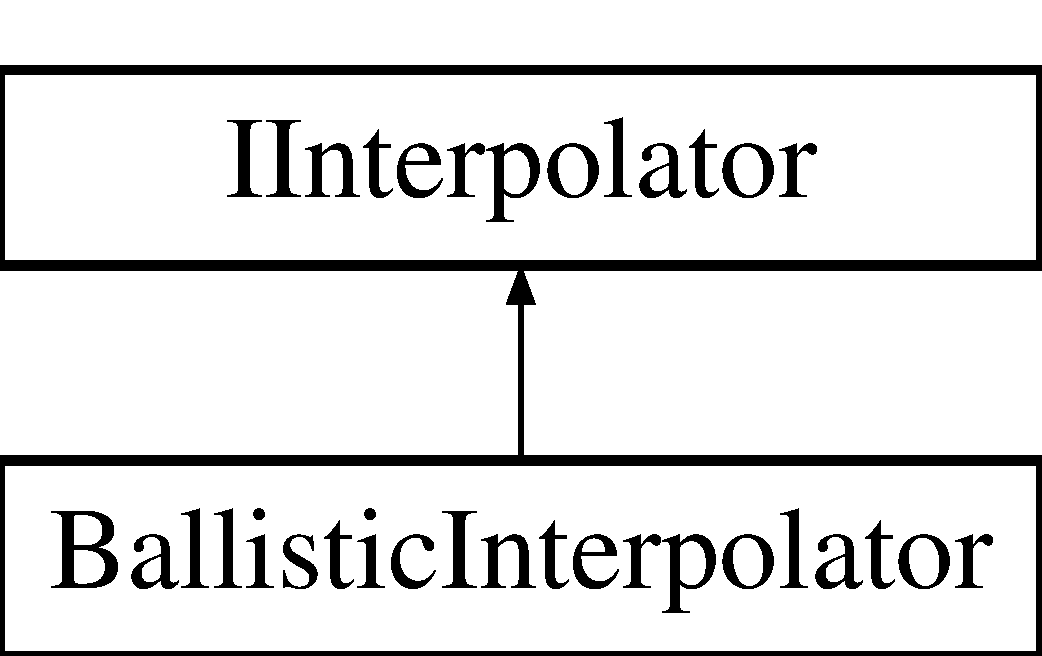
\includegraphics[height=2.000000cm]{classBallisticInterpolator}
\end{center}
\end{figure}
\subsection*{Public Member Functions}
\begin{DoxyCompactItemize}
\item 
\hypertarget{classBallisticInterpolator_ac864589b45de673ab4795618e0b83596}{{\bfseries Ballistic\-Interpolator} (\hyperlink{classVectormath_1_1Aos_1_1Vector3}{Vector3} launch, int fps)}\label{classBallisticInterpolator_ac864589b45de673ab4795618e0b83596}

\item 
\hypertarget{classBallisticInterpolator_a234becedb22f13ffdbb089e69307589d}{\hyperlink{classVectormath_1_1Aos_1_1Vector3}{Vector3} {\bfseries update} ()}\label{classBallisticInterpolator_a234becedb22f13ffdbb089e69307589d}

\end{DoxyCompactItemize}


\subsection{Detailed Description}


Definition at line 18 of file Ballistic\-Interpolator.\-h.



The documentation for this class was generated from the following files\-:\begin{DoxyCompactItemize}
\item 
src/Ballistic\-Interpolator.\-h\item 
src/Ballistic\-Interpolator.\-cpp\end{DoxyCompactItemize}

\hypertarget{classVectormath_1_1boolInVec}{\section{Vectormath\-:\-:bool\-In\-Vec Class Reference}
\label{classVectormath_1_1boolInVec}\index{Vectormath\-::bool\-In\-Vec@{Vectormath\-::bool\-In\-Vec}}
}
\subsection*{Public Member Functions}
\begin{DoxyCompactItemize}
\item 
\hypertarget{classVectormath_1_1boolInVec_aa21ebe5fd4b82622482071def03bf027}{{\bfseries bool\-In\-Vec} (\hyperlink{classVectormath_1_1floatInVec}{float\-In\-Vec} vec)}\label{classVectormath_1_1boolInVec_aa21ebe5fd4b82622482071def03bf027}

\item 
\hypertarget{classVectormath_1_1boolInVec_a4f28ddfcc232b287446eb659b2c5f326}{{\bfseries bool\-In\-Vec} (bool scalar)}\label{classVectormath_1_1boolInVec_a4f28ddfcc232b287446eb659b2c5f326}

\item 
\hypertarget{classVectormath_1_1boolInVec_a258f20bcd56f284843a5e4a0964af02a}{{\bfseries operator bool} () const }\label{classVectormath_1_1boolInVec_a258f20bcd56f284843a5e4a0964af02a}

\item 
\hypertarget{classVectormath_1_1boolInVec_a3523ca46403bfc89cc8f866a377bd26a}{vec\-\_\-uint4 {\bfseries get128} () const }\label{classVectormath_1_1boolInVec_a3523ca46403bfc89cc8f866a377bd26a}

\item 
\hypertarget{classVectormath_1_1boolInVec_aba21c8c76cb386b1d6b2c38cdabd2336}{const \hyperlink{classVectormath_1_1boolInVec}{bool\-In\-Vec} {\bfseries operator!} () const }\label{classVectormath_1_1boolInVec_aba21c8c76cb386b1d6b2c38cdabd2336}

\item 
\hypertarget{classVectormath_1_1boolInVec_a2c50cda65cc64eb8a72ccab7fc4ad88d}{\hyperlink{classVectormath_1_1boolInVec}{bool\-In\-Vec} \& {\bfseries operator=} (\hyperlink{classVectormath_1_1boolInVec}{bool\-In\-Vec} vec)}\label{classVectormath_1_1boolInVec_a2c50cda65cc64eb8a72ccab7fc4ad88d}

\item 
\hypertarget{classVectormath_1_1boolInVec_a2a14f17fa25b360c5984c491d121f446}{\hyperlink{classVectormath_1_1boolInVec}{bool\-In\-Vec} \& {\bfseries operator\&=} (\hyperlink{classVectormath_1_1boolInVec}{bool\-In\-Vec} vec)}\label{classVectormath_1_1boolInVec_a2a14f17fa25b360c5984c491d121f446}

\item 
\hypertarget{classVectormath_1_1boolInVec_ac053a8e6fee07110c9b1e963b145d47c}{\hyperlink{classVectormath_1_1boolInVec}{bool\-In\-Vec} \& {\bfseries operator$^\wedge$=} (\hyperlink{classVectormath_1_1boolInVec}{bool\-In\-Vec} vec)}\label{classVectormath_1_1boolInVec_ac053a8e6fee07110c9b1e963b145d47c}

\item 
\hypertarget{classVectormath_1_1boolInVec_ae47bc0c7ee817a201a9006b3ca99102f}{\hyperlink{classVectormath_1_1boolInVec}{bool\-In\-Vec} \& {\bfseries operator$\vert$=} (\hyperlink{classVectormath_1_1boolInVec}{bool\-In\-Vec} vec)}\label{classVectormath_1_1boolInVec_ae47bc0c7ee817a201a9006b3ca99102f}

\item 
\hypertarget{classVectormath_1_1boolInVec_aa21ebe5fd4b82622482071def03bf027}{{\bfseries bool\-In\-Vec} (\hyperlink{classVectormath_1_1floatInVec}{float\-In\-Vec} vec)}\label{classVectormath_1_1boolInVec_aa21ebe5fd4b82622482071def03bf027}

\item 
\hypertarget{classVectormath_1_1boolInVec_a4f28ddfcc232b287446eb659b2c5f326}{{\bfseries bool\-In\-Vec} (bool scalar)}\label{classVectormath_1_1boolInVec_a4f28ddfcc232b287446eb659b2c5f326}

\item 
\hypertarget{classVectormath_1_1boolInVec_a817030f4550f00989173939aaafb5958}{bool {\bfseries get\-As\-Bool} () const }\label{classVectormath_1_1boolInVec_a817030f4550f00989173939aaafb5958}

\item 
\hypertarget{classVectormath_1_1boolInVec_a258f20bcd56f284843a5e4a0964af02a}{{\bfseries operator bool} () const }\label{classVectormath_1_1boolInVec_a258f20bcd56f284843a5e4a0964af02a}

\item 
\hypertarget{classVectormath_1_1boolInVec_aba21c8c76cb386b1d6b2c38cdabd2336}{const \hyperlink{classVectormath_1_1boolInVec}{bool\-In\-Vec} {\bfseries operator!} () const }\label{classVectormath_1_1boolInVec_aba21c8c76cb386b1d6b2c38cdabd2336}

\item 
\hypertarget{classVectormath_1_1boolInVec_a50436b8ad076b8ea71a47bb30ebb84f0}{\hyperlink{classVectormath_1_1boolInVec}{bool\-In\-Vec} \& {\bfseries operator=} (\hyperlink{classVectormath_1_1boolInVec}{bool\-In\-Vec} vec)}\label{classVectormath_1_1boolInVec_a50436b8ad076b8ea71a47bb30ebb84f0}

\item 
\hypertarget{classVectormath_1_1boolInVec_a54cde71c6352419c18009930e3ae7d08}{\hyperlink{classVectormath_1_1boolInVec}{bool\-In\-Vec} \& {\bfseries operator\&=} (\hyperlink{classVectormath_1_1boolInVec}{bool\-In\-Vec} vec)}\label{classVectormath_1_1boolInVec_a54cde71c6352419c18009930e3ae7d08}

\item 
\hypertarget{classVectormath_1_1boolInVec_a816c227e73af682bc27ab3ec4dc0ba84}{\hyperlink{classVectormath_1_1boolInVec}{bool\-In\-Vec} \& {\bfseries operator$^\wedge$=} (\hyperlink{classVectormath_1_1boolInVec}{bool\-In\-Vec} vec)}\label{classVectormath_1_1boolInVec_a816c227e73af682bc27ab3ec4dc0ba84}

\item 
\hypertarget{classVectormath_1_1boolInVec_a436c4a7dd08e8a55b2496b631c3908c7}{\hyperlink{classVectormath_1_1boolInVec}{bool\-In\-Vec} \& {\bfseries operator$\vert$=} (\hyperlink{classVectormath_1_1boolInVec}{bool\-In\-Vec} vec)}\label{classVectormath_1_1boolInVec_a436c4a7dd08e8a55b2496b631c3908c7}

\item 
\hypertarget{classVectormath_1_1boolInVec_aa21ebe5fd4b82622482071def03bf027}{{\bfseries bool\-In\-Vec} (\hyperlink{classVectormath_1_1floatInVec}{float\-In\-Vec} vec)}\label{classVectormath_1_1boolInVec_aa21ebe5fd4b82622482071def03bf027}

\item 
\hypertarget{classVectormath_1_1boolInVec_a4f28ddfcc232b287446eb659b2c5f326}{{\bfseries bool\-In\-Vec} (bool scalar)}\label{classVectormath_1_1boolInVec_a4f28ddfcc232b287446eb659b2c5f326}

\item 
\hypertarget{classVectormath_1_1boolInVec_a258f20bcd56f284843a5e4a0964af02a}{{\bfseries operator bool} () const }\label{classVectormath_1_1boolInVec_a258f20bcd56f284843a5e4a0964af02a}

\item 
\hypertarget{classVectormath_1_1boolInVec_ad58ab624388d63ad6efdebde8ba46f23}{vec\-\_\-uint4 {\bfseries get128} () const }\label{classVectormath_1_1boolInVec_ad58ab624388d63ad6efdebde8ba46f23}

\item 
\hypertarget{classVectormath_1_1boolInVec_aba21c8c76cb386b1d6b2c38cdabd2336}{const \hyperlink{classVectormath_1_1boolInVec}{bool\-In\-Vec} {\bfseries operator!} () const }\label{classVectormath_1_1boolInVec_aba21c8c76cb386b1d6b2c38cdabd2336}

\item 
\hypertarget{classVectormath_1_1boolInVec_a50436b8ad076b8ea71a47bb30ebb84f0}{\hyperlink{classVectormath_1_1boolInVec}{bool\-In\-Vec} \& {\bfseries operator=} (\hyperlink{classVectormath_1_1boolInVec}{bool\-In\-Vec} vec)}\label{classVectormath_1_1boolInVec_a50436b8ad076b8ea71a47bb30ebb84f0}

\item 
\hypertarget{classVectormath_1_1boolInVec_a54cde71c6352419c18009930e3ae7d08}{\hyperlink{classVectormath_1_1boolInVec}{bool\-In\-Vec} \& {\bfseries operator\&=} (\hyperlink{classVectormath_1_1boolInVec}{bool\-In\-Vec} vec)}\label{classVectormath_1_1boolInVec_a54cde71c6352419c18009930e3ae7d08}

\item 
\hypertarget{classVectormath_1_1boolInVec_a816c227e73af682bc27ab3ec4dc0ba84}{\hyperlink{classVectormath_1_1boolInVec}{bool\-In\-Vec} \& {\bfseries operator$^\wedge$=} (\hyperlink{classVectormath_1_1boolInVec}{bool\-In\-Vec} vec)}\label{classVectormath_1_1boolInVec_a816c227e73af682bc27ab3ec4dc0ba84}

\item 
\hypertarget{classVectormath_1_1boolInVec_a436c4a7dd08e8a55b2496b631c3908c7}{\hyperlink{classVectormath_1_1boolInVec}{bool\-In\-Vec} \& {\bfseries operator$\vert$=} (\hyperlink{classVectormath_1_1boolInVec}{bool\-In\-Vec} vec)}\label{classVectormath_1_1boolInVec_a436c4a7dd08e8a55b2496b631c3908c7}

\item 
\hypertarget{classVectormath_1_1boolInVec_a8ef3cf4d747e40bbfd938fc2cc45e47a}{{\bfseries bool\-In\-Vec} (const \hyperlink{classVectormath_1_1floatInVec}{float\-In\-Vec} \&vec)}\label{classVectormath_1_1boolInVec_a8ef3cf4d747e40bbfd938fc2cc45e47a}

\item 
\hypertarget{classVectormath_1_1boolInVec_a4f28ddfcc232b287446eb659b2c5f326}{{\bfseries bool\-In\-Vec} (bool scalar)}\label{classVectormath_1_1boolInVec_a4f28ddfcc232b287446eb659b2c5f326}

\item 
\hypertarget{classVectormath_1_1boolInVec_a258f20bcd56f284843a5e4a0964af02a}{{\bfseries operator bool} () const }\label{classVectormath_1_1boolInVec_a258f20bcd56f284843a5e4a0964af02a}

\item 
\hypertarget{classVectormath_1_1boolInVec_a3523ca46403bfc89cc8f866a377bd26a}{\-\_\-\-\_\-m128 {\bfseries get128} () const }\label{classVectormath_1_1boolInVec_a3523ca46403bfc89cc8f866a377bd26a}

\item 
\hypertarget{classVectormath_1_1boolInVec_aba21c8c76cb386b1d6b2c38cdabd2336}{const \hyperlink{classVectormath_1_1boolInVec}{bool\-In\-Vec} {\bfseries operator!} () const }\label{classVectormath_1_1boolInVec_aba21c8c76cb386b1d6b2c38cdabd2336}

\item 
\hypertarget{classVectormath_1_1boolInVec_a36c75606d50f8e325c7fb34532fd415a}{\hyperlink{classVectormath_1_1boolInVec}{bool\-In\-Vec} \& {\bfseries operator=} (const \hyperlink{classVectormath_1_1boolInVec}{bool\-In\-Vec} \&vec)}\label{classVectormath_1_1boolInVec_a36c75606d50f8e325c7fb34532fd415a}

\item 
\hypertarget{classVectormath_1_1boolInVec_ac7479e8053214630cde5be566fa5ee14}{\hyperlink{classVectormath_1_1boolInVec}{bool\-In\-Vec} \& {\bfseries operator\&=} (const \hyperlink{classVectormath_1_1boolInVec}{bool\-In\-Vec} \&vec)}\label{classVectormath_1_1boolInVec_ac7479e8053214630cde5be566fa5ee14}

\item 
\hypertarget{classVectormath_1_1boolInVec_a8915a03317c76504ea94862ff67d3afc}{\hyperlink{classVectormath_1_1boolInVec}{bool\-In\-Vec} \& {\bfseries operator$^\wedge$=} (const \hyperlink{classVectormath_1_1boolInVec}{bool\-In\-Vec} \&vec)}\label{classVectormath_1_1boolInVec_a8915a03317c76504ea94862ff67d3afc}

\item 
\hypertarget{classVectormath_1_1boolInVec_a35c9158395ce7b3162ebb4f1ef7fa323}{\hyperlink{classVectormath_1_1boolInVec}{bool\-In\-Vec} \& {\bfseries operator$\vert$=} (const \hyperlink{classVectormath_1_1boolInVec}{bool\-In\-Vec} \&vec)}\label{classVectormath_1_1boolInVec_a35c9158395ce7b3162ebb4f1ef7fa323}

\end{DoxyCompactItemize}
\subsection*{Friends}
\begin{DoxyCompactItemize}
\item 
\hypertarget{classVectormath_1_1boolInVec_a17636a41b47891b2af6f18af607785fb}{const \hyperlink{classVectormath_1_1boolInVec}{bool\-In\-Vec} {\bfseries operator==} (\hyperlink{classVectormath_1_1boolInVec}{bool\-In\-Vec} vec0, \hyperlink{classVectormath_1_1boolInVec}{bool\-In\-Vec} vec1)}\label{classVectormath_1_1boolInVec_a17636a41b47891b2af6f18af607785fb}

\item 
\hypertarget{classVectormath_1_1boolInVec_a02c7bd413b9523c8998268b9410c3d3f}{const \hyperlink{classVectormath_1_1boolInVec}{bool\-In\-Vec} {\bfseries operator!=} (\hyperlink{classVectormath_1_1boolInVec}{bool\-In\-Vec} vec0, \hyperlink{classVectormath_1_1boolInVec}{bool\-In\-Vec} vec1)}\label{classVectormath_1_1boolInVec_a02c7bd413b9523c8998268b9410c3d3f}

\item 
\hypertarget{classVectormath_1_1boolInVec_a45be682c5b8d9d67a3ac2f9499b5b9fa}{const \hyperlink{classVectormath_1_1boolInVec}{bool\-In\-Vec} {\bfseries operator$<$} (\hyperlink{classVectormath_1_1floatInVec}{float\-In\-Vec} vec0, \hyperlink{classVectormath_1_1floatInVec}{float\-In\-Vec} vec1)}\label{classVectormath_1_1boolInVec_a45be682c5b8d9d67a3ac2f9499b5b9fa}

\item 
\hypertarget{classVectormath_1_1boolInVec_a47d71eec700bac5d004e309f26d52515}{const \hyperlink{classVectormath_1_1boolInVec}{bool\-In\-Vec} {\bfseries operator$<$=} (\hyperlink{classVectormath_1_1floatInVec}{float\-In\-Vec} vec0, \hyperlink{classVectormath_1_1floatInVec}{float\-In\-Vec} vec1)}\label{classVectormath_1_1boolInVec_a47d71eec700bac5d004e309f26d52515}

\item 
\hypertarget{classVectormath_1_1boolInVec_aa77a870a79fdc7d8d9ce861c467cf45d}{const \hyperlink{classVectormath_1_1boolInVec}{bool\-In\-Vec} {\bfseries operator$>$} (\hyperlink{classVectormath_1_1floatInVec}{float\-In\-Vec} vec0, \hyperlink{classVectormath_1_1floatInVec}{float\-In\-Vec} vec1)}\label{classVectormath_1_1boolInVec_aa77a870a79fdc7d8d9ce861c467cf45d}

\item 
\hypertarget{classVectormath_1_1boolInVec_a50a1d091ec4daabc05d4ebb1d8393599}{const \hyperlink{classVectormath_1_1boolInVec}{bool\-In\-Vec} {\bfseries operator$>$=} (\hyperlink{classVectormath_1_1floatInVec}{float\-In\-Vec} vec0, \hyperlink{classVectormath_1_1floatInVec}{float\-In\-Vec} vec1)}\label{classVectormath_1_1boolInVec_a50a1d091ec4daabc05d4ebb1d8393599}

\item 
\hypertarget{classVectormath_1_1boolInVec_a28324adfe9227010621c32882250fa88}{const \hyperlink{classVectormath_1_1boolInVec}{bool\-In\-Vec} {\bfseries operator==} (\hyperlink{classVectormath_1_1floatInVec}{float\-In\-Vec} vec0, \hyperlink{classVectormath_1_1floatInVec}{float\-In\-Vec} vec1)}\label{classVectormath_1_1boolInVec_a28324adfe9227010621c32882250fa88}

\item 
\hypertarget{classVectormath_1_1boolInVec_aa8981ea9f4671fbd35f36bf3d41e0cdc}{const \hyperlink{classVectormath_1_1boolInVec}{bool\-In\-Vec} {\bfseries operator!=} (\hyperlink{classVectormath_1_1floatInVec}{float\-In\-Vec} vec0, \hyperlink{classVectormath_1_1floatInVec}{float\-In\-Vec} vec1)}\label{classVectormath_1_1boolInVec_aa8981ea9f4671fbd35f36bf3d41e0cdc}

\item 
\hypertarget{classVectormath_1_1boolInVec_a01dbf38fde081c4a09b3c211096c65bd}{const \hyperlink{classVectormath_1_1boolInVec}{bool\-In\-Vec} {\bfseries operator\&} (\hyperlink{classVectormath_1_1boolInVec}{bool\-In\-Vec} vec0, \hyperlink{classVectormath_1_1boolInVec}{bool\-In\-Vec} vec1)}\label{classVectormath_1_1boolInVec_a01dbf38fde081c4a09b3c211096c65bd}

\item 
\hypertarget{classVectormath_1_1boolInVec_a656e8a73823c6513e4ba4953ab643f35}{const \hyperlink{classVectormath_1_1boolInVec}{bool\-In\-Vec} {\bfseries operator$^\wedge$} (\hyperlink{classVectormath_1_1boolInVec}{bool\-In\-Vec} vec0, \hyperlink{classVectormath_1_1boolInVec}{bool\-In\-Vec} vec1)}\label{classVectormath_1_1boolInVec_a656e8a73823c6513e4ba4953ab643f35}

\item 
\hypertarget{classVectormath_1_1boolInVec_ac8b957e796b0ed158f7302726d892ff9}{const \hyperlink{classVectormath_1_1boolInVec}{bool\-In\-Vec} {\bfseries operator$\vert$} (\hyperlink{classVectormath_1_1boolInVec}{bool\-In\-Vec} vec0, \hyperlink{classVectormath_1_1boolInVec}{bool\-In\-Vec} vec1)}\label{classVectormath_1_1boolInVec_ac8b957e796b0ed158f7302726d892ff9}

\item 
\hypertarget{classVectormath_1_1boolInVec_a0593cfee6ee3c5a6eae4a715b26b39c8}{const \hyperlink{classVectormath_1_1boolInVec}{bool\-In\-Vec} {\bfseries select} (\hyperlink{classVectormath_1_1boolInVec}{bool\-In\-Vec} vec0, \hyperlink{classVectormath_1_1boolInVec}{bool\-In\-Vec} vec1, \hyperlink{classVectormath_1_1boolInVec}{bool\-In\-Vec} select\-\_\-vec1)}\label{classVectormath_1_1boolInVec_a0593cfee6ee3c5a6eae4a715b26b39c8}

\item 
\hypertarget{classVectormath_1_1boolInVec_a17636a41b47891b2af6f18af607785fb}{const \hyperlink{classVectormath_1_1boolInVec}{bool\-In\-Vec} {\bfseries operator==} (\hyperlink{classVectormath_1_1boolInVec}{bool\-In\-Vec} vec0, \hyperlink{classVectormath_1_1boolInVec}{bool\-In\-Vec} vec1)}\label{classVectormath_1_1boolInVec_a17636a41b47891b2af6f18af607785fb}

\item 
\hypertarget{classVectormath_1_1boolInVec_a02c7bd413b9523c8998268b9410c3d3f}{const \hyperlink{classVectormath_1_1boolInVec}{bool\-In\-Vec} {\bfseries operator!=} (\hyperlink{classVectormath_1_1boolInVec}{bool\-In\-Vec} vec0, \hyperlink{classVectormath_1_1boolInVec}{bool\-In\-Vec} vec1)}\label{classVectormath_1_1boolInVec_a02c7bd413b9523c8998268b9410c3d3f}

\item 
\hypertarget{classVectormath_1_1boolInVec_a45be682c5b8d9d67a3ac2f9499b5b9fa}{const \hyperlink{classVectormath_1_1boolInVec}{bool\-In\-Vec} {\bfseries operator$<$} (\hyperlink{classVectormath_1_1floatInVec}{float\-In\-Vec} vec0, \hyperlink{classVectormath_1_1floatInVec}{float\-In\-Vec} vec1)}\label{classVectormath_1_1boolInVec_a45be682c5b8d9d67a3ac2f9499b5b9fa}

\item 
\hypertarget{classVectormath_1_1boolInVec_a47d71eec700bac5d004e309f26d52515}{const \hyperlink{classVectormath_1_1boolInVec}{bool\-In\-Vec} {\bfseries operator$<$=} (\hyperlink{classVectormath_1_1floatInVec}{float\-In\-Vec} vec0, \hyperlink{classVectormath_1_1floatInVec}{float\-In\-Vec} vec1)}\label{classVectormath_1_1boolInVec_a47d71eec700bac5d004e309f26d52515}

\item 
\hypertarget{classVectormath_1_1boolInVec_aa77a870a79fdc7d8d9ce861c467cf45d}{const \hyperlink{classVectormath_1_1boolInVec}{bool\-In\-Vec} {\bfseries operator$>$} (\hyperlink{classVectormath_1_1floatInVec}{float\-In\-Vec} vec0, \hyperlink{classVectormath_1_1floatInVec}{float\-In\-Vec} vec1)}\label{classVectormath_1_1boolInVec_aa77a870a79fdc7d8d9ce861c467cf45d}

\item 
\hypertarget{classVectormath_1_1boolInVec_a50a1d091ec4daabc05d4ebb1d8393599}{const \hyperlink{classVectormath_1_1boolInVec}{bool\-In\-Vec} {\bfseries operator$>$=} (\hyperlink{classVectormath_1_1floatInVec}{float\-In\-Vec} vec0, \hyperlink{classVectormath_1_1floatInVec}{float\-In\-Vec} vec1)}\label{classVectormath_1_1boolInVec_a50a1d091ec4daabc05d4ebb1d8393599}

\item 
\hypertarget{classVectormath_1_1boolInVec_a28324adfe9227010621c32882250fa88}{const \hyperlink{classVectormath_1_1boolInVec}{bool\-In\-Vec} {\bfseries operator==} (\hyperlink{classVectormath_1_1floatInVec}{float\-In\-Vec} vec0, \hyperlink{classVectormath_1_1floatInVec}{float\-In\-Vec} vec1)}\label{classVectormath_1_1boolInVec_a28324adfe9227010621c32882250fa88}

\item 
\hypertarget{classVectormath_1_1boolInVec_aa8981ea9f4671fbd35f36bf3d41e0cdc}{const \hyperlink{classVectormath_1_1boolInVec}{bool\-In\-Vec} {\bfseries operator!=} (\hyperlink{classVectormath_1_1floatInVec}{float\-In\-Vec} vec0, \hyperlink{classVectormath_1_1floatInVec}{float\-In\-Vec} vec1)}\label{classVectormath_1_1boolInVec_aa8981ea9f4671fbd35f36bf3d41e0cdc}

\item 
\hypertarget{classVectormath_1_1boolInVec_a01dbf38fde081c4a09b3c211096c65bd}{const \hyperlink{classVectormath_1_1boolInVec}{bool\-In\-Vec} {\bfseries operator\&} (\hyperlink{classVectormath_1_1boolInVec}{bool\-In\-Vec} vec0, \hyperlink{classVectormath_1_1boolInVec}{bool\-In\-Vec} vec1)}\label{classVectormath_1_1boolInVec_a01dbf38fde081c4a09b3c211096c65bd}

\item 
\hypertarget{classVectormath_1_1boolInVec_a656e8a73823c6513e4ba4953ab643f35}{const \hyperlink{classVectormath_1_1boolInVec}{bool\-In\-Vec} {\bfseries operator$^\wedge$} (\hyperlink{classVectormath_1_1boolInVec}{bool\-In\-Vec} vec0, \hyperlink{classVectormath_1_1boolInVec}{bool\-In\-Vec} vec1)}\label{classVectormath_1_1boolInVec_a656e8a73823c6513e4ba4953ab643f35}

\item 
\hypertarget{classVectormath_1_1boolInVec_ac8b957e796b0ed158f7302726d892ff9}{const \hyperlink{classVectormath_1_1boolInVec}{bool\-In\-Vec} {\bfseries operator$\vert$} (\hyperlink{classVectormath_1_1boolInVec}{bool\-In\-Vec} vec0, \hyperlink{classVectormath_1_1boolInVec}{bool\-In\-Vec} vec1)}\label{classVectormath_1_1boolInVec_ac8b957e796b0ed158f7302726d892ff9}

\item 
\hypertarget{classVectormath_1_1boolInVec_a0593cfee6ee3c5a6eae4a715b26b39c8}{const \hyperlink{classVectormath_1_1boolInVec}{bool\-In\-Vec} {\bfseries select} (\hyperlink{classVectormath_1_1boolInVec}{bool\-In\-Vec} vec0, \hyperlink{classVectormath_1_1boolInVec}{bool\-In\-Vec} vec1, \hyperlink{classVectormath_1_1boolInVec}{bool\-In\-Vec} select\-\_\-vec1)}\label{classVectormath_1_1boolInVec_a0593cfee6ee3c5a6eae4a715b26b39c8}

\item 
\hypertarget{classVectormath_1_1boolInVec_af7f7c8557b1401381f6ef219bbcf1507}{const \hyperlink{classVectormath_1_1boolInVec}{bool\-In\-Vec} {\bfseries operator==} (const \hyperlink{classVectormath_1_1boolInVec}{bool\-In\-Vec} \&vec0, const \hyperlink{classVectormath_1_1boolInVec}{bool\-In\-Vec} \&vec1)}\label{classVectormath_1_1boolInVec_af7f7c8557b1401381f6ef219bbcf1507}

\item 
\hypertarget{classVectormath_1_1boolInVec_a7b3be8b2f8064495dba70f7e7ba3f47b}{const \hyperlink{classVectormath_1_1boolInVec}{bool\-In\-Vec} {\bfseries operator!=} (const \hyperlink{classVectormath_1_1boolInVec}{bool\-In\-Vec} \&vec0, const \hyperlink{classVectormath_1_1boolInVec}{bool\-In\-Vec} \&vec1)}\label{classVectormath_1_1boolInVec_a7b3be8b2f8064495dba70f7e7ba3f47b}

\item 
\hypertarget{classVectormath_1_1boolInVec_aaf77cbfadf0d6df54184580f9b38fee2}{const \hyperlink{classVectormath_1_1boolInVec}{bool\-In\-Vec} {\bfseries operator$<$} (const \hyperlink{classVectormath_1_1floatInVec}{float\-In\-Vec} \&vec0, const \hyperlink{classVectormath_1_1floatInVec}{float\-In\-Vec} \&vec1)}\label{classVectormath_1_1boolInVec_aaf77cbfadf0d6df54184580f9b38fee2}

\item 
\hypertarget{classVectormath_1_1boolInVec_a7de5fdb3a4cc2be5508e070d9e202281}{const \hyperlink{classVectormath_1_1boolInVec}{bool\-In\-Vec} {\bfseries operator$<$=} (const \hyperlink{classVectormath_1_1floatInVec}{float\-In\-Vec} \&vec0, const \hyperlink{classVectormath_1_1floatInVec}{float\-In\-Vec} \&vec1)}\label{classVectormath_1_1boolInVec_a7de5fdb3a4cc2be5508e070d9e202281}

\item 
\hypertarget{classVectormath_1_1boolInVec_a2788b1aa4c31b395cc822e833383cea0}{const \hyperlink{classVectormath_1_1boolInVec}{bool\-In\-Vec} {\bfseries operator$>$} (const \hyperlink{classVectormath_1_1floatInVec}{float\-In\-Vec} \&vec0, const \hyperlink{classVectormath_1_1floatInVec}{float\-In\-Vec} \&vec1)}\label{classVectormath_1_1boolInVec_a2788b1aa4c31b395cc822e833383cea0}

\item 
\hypertarget{classVectormath_1_1boolInVec_a66d1f66087d68bf150249d39bd19a28d}{const \hyperlink{classVectormath_1_1boolInVec}{bool\-In\-Vec} {\bfseries operator$>$=} (const \hyperlink{classVectormath_1_1floatInVec}{float\-In\-Vec} \&vec0, const \hyperlink{classVectormath_1_1floatInVec}{float\-In\-Vec} \&vec1)}\label{classVectormath_1_1boolInVec_a66d1f66087d68bf150249d39bd19a28d}

\item 
\hypertarget{classVectormath_1_1boolInVec_a0c3d1d83ce1a894626a8d4265a5f2ed9}{const \hyperlink{classVectormath_1_1boolInVec}{bool\-In\-Vec} {\bfseries operator==} (const \hyperlink{classVectormath_1_1floatInVec}{float\-In\-Vec} \&vec0, const \hyperlink{classVectormath_1_1floatInVec}{float\-In\-Vec} \&vec1)}\label{classVectormath_1_1boolInVec_a0c3d1d83ce1a894626a8d4265a5f2ed9}

\item 
\hypertarget{classVectormath_1_1boolInVec_a4d52df8e4badb8a75fc9bc565a86ad94}{const \hyperlink{classVectormath_1_1boolInVec}{bool\-In\-Vec} {\bfseries operator!=} (const \hyperlink{classVectormath_1_1floatInVec}{float\-In\-Vec} \&vec0, const \hyperlink{classVectormath_1_1floatInVec}{float\-In\-Vec} \&vec1)}\label{classVectormath_1_1boolInVec_a4d52df8e4badb8a75fc9bc565a86ad94}

\item 
\hypertarget{classVectormath_1_1boolInVec_a74ccbd8738ab84dc5be0ed51cc6377f3}{const \hyperlink{classVectormath_1_1boolInVec}{bool\-In\-Vec} {\bfseries operator\&} (const \hyperlink{classVectormath_1_1boolInVec}{bool\-In\-Vec} \&vec0, const \hyperlink{classVectormath_1_1boolInVec}{bool\-In\-Vec} \&vec1)}\label{classVectormath_1_1boolInVec_a74ccbd8738ab84dc5be0ed51cc6377f3}

\item 
\hypertarget{classVectormath_1_1boolInVec_a5c92593983de1257dafe7301c6665108}{const \hyperlink{classVectormath_1_1boolInVec}{bool\-In\-Vec} {\bfseries operator$^\wedge$} (const \hyperlink{classVectormath_1_1boolInVec}{bool\-In\-Vec} \&vec0, const \hyperlink{classVectormath_1_1boolInVec}{bool\-In\-Vec} \&vec1)}\label{classVectormath_1_1boolInVec_a5c92593983de1257dafe7301c6665108}

\item 
\hypertarget{classVectormath_1_1boolInVec_a33e35c11ed0093bc8949a434da600031}{const \hyperlink{classVectormath_1_1boolInVec}{bool\-In\-Vec} {\bfseries operator$\vert$} (const \hyperlink{classVectormath_1_1boolInVec}{bool\-In\-Vec} \&vec0, const \hyperlink{classVectormath_1_1boolInVec}{bool\-In\-Vec} \&vec1)}\label{classVectormath_1_1boolInVec_a33e35c11ed0093bc8949a434da600031}

\item 
\hypertarget{classVectormath_1_1boolInVec_ac6cfb2aee5afd68adfddecc9f41d915b}{const \hyperlink{classVectormath_1_1boolInVec}{bool\-In\-Vec} {\bfseries select} (const \hyperlink{classVectormath_1_1boolInVec}{bool\-In\-Vec} \&vec0, const \hyperlink{classVectormath_1_1boolInVec}{bool\-In\-Vec} \&vec1, const \hyperlink{classVectormath_1_1boolInVec}{bool\-In\-Vec} \&select\-\_\-vec1)}\label{classVectormath_1_1boolInVec_ac6cfb2aee5afd68adfddecc9f41d915b}

\end{DoxyCompactItemize}


\subsection{Detailed Description}


Definition at line 46 of file bool\-In\-Vec.\-h.



The documentation for this class was generated from the following file\-:\begin{DoxyCompactItemize}
\item 
src/include/vectormath/ppu/cpp/bool\-In\-Vec.\-h\end{DoxyCompactItemize}

\hypertarget{classBoundingBox}{\section{Bounding\-Box Class Reference}
\label{classBoundingBox}\index{Bounding\-Box@{Bounding\-Box}}
}


Bounding Box Class.  




{\ttfamily \#include $<$Bounding\-Box.\-h$>$}

\subsection*{Public Member Functions}
\begin{DoxyCompactItemize}
\item 
\hypertarget{classBoundingBox_af06000fc84c707ac6fc5451c63de3480}{{\bfseries Bounding\-Box} (const \hyperlink{classVectormath_1_1Aos_1_1Point3}{Point3} \&c, const float extent\-\_\-x, const float extent\-\_\-y, const float extent\-\_\-z)}\label{classBoundingBox_af06000fc84c707ac6fc5451c63de3480}

\item 
bool \hyperlink{classBoundingBox_a90418b763701826c706178845903dd7c}{collides\-With} (const \hyperlink{classBoundingBox}{Bounding\-Box} \&b)
\begin{DoxyCompactList}\small\item\em Collision method. \end{DoxyCompactList}\item 
pair$<$ float, float $>$ \hyperlink{classBoundingBox_a20a8d578fbfd1702e183921f9ec0a0d2}{project\-Onto\-Axis} (const \hyperlink{classBoundingBox}{Bounding\-Box} \&b, enum A\-X\-I\-S)
\item 
shared\-\_\-ptr$<$ \hyperlink{classVectormath_1_1Aos_1_1Point3}{Point3} $>$ \hyperlink{classBoundingBox_aceef7769498825680d34638bccc6f490}{get\-Centre} ()
\end{DoxyCompactItemize}


\subsection{Detailed Description}
Bounding Box Class. 

A simple box used in collision detection. 

Definition at line 31 of file Bounding\-Box.\-h.



\subsection{Member Function Documentation}
\hypertarget{classBoundingBox_a90418b763701826c706178845903dd7c}{\index{Bounding\-Box@{Bounding\-Box}!collides\-With@{collides\-With}}
\index{collides\-With@{collides\-With}!BoundingBox@{Bounding\-Box}}
\subsubsection[{collides\-With}]{\setlength{\rightskip}{0pt plus 5cm}bool Bounding\-Box\-::collides\-With (
\begin{DoxyParamCaption}
\item[{const {\bf Bounding\-Box} \&}]{b}
\end{DoxyParamCaption}
)}}\label{classBoundingBox_a90418b763701826c706178845903dd7c}


Collision method. 

Tests for a collision between this and the given Bounding\-Boxs 

Definition at line 26 of file Bounding\-Box.\-cpp.

\hypertarget{classBoundingBox_aceef7769498825680d34638bccc6f490}{\index{Bounding\-Box@{Bounding\-Box}!get\-Centre@{get\-Centre}}
\index{get\-Centre@{get\-Centre}!BoundingBox@{Bounding\-Box}}
\subsubsection[{get\-Centre}]{\setlength{\rightskip}{0pt plus 5cm}shared\-\_\-ptr$<$ {\bf Point3} $>$ Bounding\-Box\-::get\-Centre (
\begin{DoxyParamCaption}
{}
\end{DoxyParamCaption}
)}}\label{classBoundingBox_aceef7769498825680d34638bccc6f490}
Gets the \hyperlink{classBoundingBox}{Bounding\-Box}'s centre. 

Definition at line 61 of file Bounding\-Box.\-cpp.

\hypertarget{classBoundingBox_a20a8d578fbfd1702e183921f9ec0a0d2}{\index{Bounding\-Box@{Bounding\-Box}!project\-Onto\-Axis@{project\-Onto\-Axis}}
\index{project\-Onto\-Axis@{project\-Onto\-Axis}!BoundingBox@{Bounding\-Box}}
\subsubsection[{project\-Onto\-Axis}]{\setlength{\rightskip}{0pt plus 5cm}pair$<$ float, float $>$ Bounding\-Box\-::project\-Onto\-Axis (
\begin{DoxyParamCaption}
\item[{const {\bf Bounding\-Box} \&}]{b, }
\item[{enum A\-X\-I\-S}]{axis}
\end{DoxyParamCaption}
)}}\label{classBoundingBox_a20a8d578fbfd1702e183921f9ec0a0d2}
Part of collision method, used to compare values on 1 axis only. 

Definition at line 39 of file Bounding\-Box.\-cpp.



The documentation for this class was generated from the following files\-:\begin{DoxyCompactItemize}
\item 
src/Bounding\-Box.\-h\item 
src/Bounding\-Box.\-cpp\end{DoxyCompactItemize}

\hypertarget{classCamera}{\section{Camera Class Reference}
\label{classCamera}\index{Camera@{Camera}}
}


\hyperlink{classCamera}{Camera} class.  




{\ttfamily \#include $<$Camera.\-h$>$}

\subsection*{Public Member Functions}
\begin{DoxyCompactItemize}
\item 
virtual \hyperlink{classCamera_ad1897942d0ccf91052386388a497349f}{$\sim$\-Camera} ()
\item 
void \hyperlink{classCamera_a16c5e6f7b2eed95a78675f55c4a435e6}{set\-Camera} (const \hyperlink{classVectormath_1_1Aos_1_1Matrix4}{Matrix4} \&m)
\item 
void \hyperlink{classCamera_aa91c4a447f23e08322ef17f2786851bf}{look\-At} (const \hyperlink{classVectormath_1_1Aos_1_1Point3}{Point3} \&eye, const \hyperlink{classVectormath_1_1Aos_1_1Point3}{Point3} \&point, const \hyperlink{classVectormath_1_1Aos_1_1Vector3}{Vector3} \&up)
\item 
float $\ast$ \hyperlink{classCamera_a25f2f9d8ccc76f38c0580709587afadf}{get\-Camera} ()
\item 
\hyperlink{classVectormath_1_1Aos_1_1Matrix4}{Matrix4} \& \hyperlink{classCamera_a156b6aba4309cde6f0252ff325663e2f}{get\-Camera\-M} ()
\end{DoxyCompactItemize}
\subsection*{Static Public Member Functions}
\begin{DoxyCompactItemize}
\item 
static \hyperlink{classCamera}{Camera} \& \hyperlink{classCamera_aa84baebe5d771ddfd82a5b55bd3fde39}{get\-Instance} ()
\end{DoxyCompactItemize}


\subsection{Detailed Description}
\hyperlink{classCamera}{Camera} class. 

Stores a 4x4 Matrix to transform the world and changes the Matrix as appropriate when the camera moves. 

Definition at line 22 of file Camera.\-h.



\subsection{Constructor \& Destructor Documentation}
\hypertarget{classCamera_ad1897942d0ccf91052386388a497349f}{\index{Camera@{Camera}!$\sim$\-Camera@{$\sim$\-Camera}}
\index{$\sim$\-Camera@{$\sim$\-Camera}!Camera@{Camera}}
\subsubsection[{$\sim$\-Camera}]{\setlength{\rightskip}{0pt plus 5cm}Camera\-::$\sim$\-Camera (
\begin{DoxyParamCaption}
{}
\end{DoxyParamCaption}
)\hspace{0.3cm}{\ttfamily [virtual]}}}\label{classCamera_ad1897942d0ccf91052386388a497349f}
Not implemented. 

Definition at line 13 of file Camera.\-cpp.



\subsection{Member Function Documentation}
\hypertarget{classCamera_a25f2f9d8ccc76f38c0580709587afadf}{\index{Camera@{Camera}!get\-Camera@{get\-Camera}}
\index{get\-Camera@{get\-Camera}!Camera@{Camera}}
\subsubsection[{get\-Camera}]{\setlength{\rightskip}{0pt plus 5cm}float $\ast$ Camera\-::get\-Camera (
\begin{DoxyParamCaption}
{}
\end{DoxyParamCaption}
)}}\label{classCamera_a25f2f9d8ccc76f38c0580709587afadf}
Returns the \hyperlink{classCamera}{Camera}'s 4x4 Matrix as an array of floats 

Definition at line 27 of file Camera.\-cpp.

\hypertarget{classCamera_a156b6aba4309cde6f0252ff325663e2f}{\index{Camera@{Camera}!get\-Camera\-M@{get\-Camera\-M}}
\index{get\-Camera\-M@{get\-Camera\-M}!Camera@{Camera}}
\subsubsection[{get\-Camera\-M}]{\setlength{\rightskip}{0pt plus 5cm}{\bf Matrix4} \& Camera\-::get\-Camera\-M (
\begin{DoxyParamCaption}
{}
\end{DoxyParamCaption}
)}}\label{classCamera_a156b6aba4309cde6f0252ff325663e2f}
Returns the \hyperlink{classCamera}{Camera}'s 4x4 Matrix 

Definition at line 51 of file Camera.\-cpp.

\hypertarget{classCamera_aa84baebe5d771ddfd82a5b55bd3fde39}{\index{Camera@{Camera}!get\-Instance@{get\-Instance}}
\index{get\-Instance@{get\-Instance}!Camera@{Camera}}
\subsubsection[{get\-Instance}]{\setlength{\rightskip}{0pt plus 5cm}{\bf Camera} \& Camera\-::get\-Instance (
\begin{DoxyParamCaption}
{}
\end{DoxyParamCaption}
)\hspace{0.3cm}{\ttfamily [static]}}}\label{classCamera_aa84baebe5d771ddfd82a5b55bd3fde39}
Creates itself if undefined and returns itself. 

Definition at line 55 of file Camera.\-cpp.

\hypertarget{classCamera_aa91c4a447f23e08322ef17f2786851bf}{\index{Camera@{Camera}!look\-At@{look\-At}}
\index{look\-At@{look\-At}!Camera@{Camera}}
\subsubsection[{look\-At}]{\setlength{\rightskip}{0pt plus 5cm}void Camera\-::look\-At (
\begin{DoxyParamCaption}
\item[{const {\bf Point3} \&}]{eye, }
\item[{const {\bf Point3} \&}]{point, }
\item[{const {\bf Vector3} \&}]{up}
\end{DoxyParamCaption}
)}}\label{classCamera_aa91c4a447f23e08322ef17f2786851bf}
Changes the \hyperlink{classCamera}{Camera}'s 4x4 Matrix to the one returned by Matrix4's look\-At method. 

Definition at line 17 of file Camera.\-cpp.

\hypertarget{classCamera_a16c5e6f7b2eed95a78675f55c4a435e6}{\index{Camera@{Camera}!set\-Camera@{set\-Camera}}
\index{set\-Camera@{set\-Camera}!Camera@{Camera}}
\subsubsection[{set\-Camera}]{\setlength{\rightskip}{0pt plus 5cm}void Camera\-::set\-Camera (
\begin{DoxyParamCaption}
\item[{const {\bf Matrix4} \&}]{m}
\end{DoxyParamCaption}
)}}\label{classCamera_a16c5e6f7b2eed95a78675f55c4a435e6}
Changes the \hyperlink{classCamera}{Camera}'s 4x4 Matrix to the one given. 

Definition at line 21 of file Camera.\-cpp.



The documentation for this class was generated from the following files\-:\begin{DoxyCompactItemize}
\item 
src/Camera.\-h\item 
src/Camera.\-cpp\end{DoxyCompactItemize}

\hypertarget{classController}{\section{Controller Class Reference}
\label{classController}\index{Controller@{Controller}}
}


\hyperlink{classController}{Controller} Class.  




{\ttfamily \#include $<$Controller.\-h$>$}

\subsection*{Public Member Functions}
\begin{DoxyCompactItemize}
\item 
\hyperlink{classController_a1528d018e9f08fe261455d427efd1d2f}{Controller} (\hyperlink{classData}{Data} $\ast$d, \hyperlink{classPhysics}{Physics} $\ast$p)
\begin{DoxyCompactList}\small\item\em Constructor. \end{DoxyCompactList}\item 
void \hyperlink{classController_a96c6647ef20bf9425ca1704fc5e78d2f}{m\-Move\-Events} (S\-D\-L\-\_\-\-Event \&event)
\begin{DoxyCompactList}\small\item\em Move Mouse Event Handler. \end{DoxyCompactList}\item 
void \hyperlink{classController_a6037d971c6636f752aca1cd099ba0d33}{k\-Down\-Events} (S\-D\-L\-\_\-\-Event \&event)
\begin{DoxyCompactList}\small\item\em Key Down Event Handler. \end{DoxyCompactList}\end{DoxyCompactItemize}


\subsection{Detailed Description}
\hyperlink{classController}{Controller} Class. 

A simple class that handles Mouse and Keyboard events. 

Definition at line 29 of file Controller.\-h.



\subsection{Constructor \& Destructor Documentation}
\hypertarget{classController_a1528d018e9f08fe261455d427efd1d2f}{\index{Controller@{Controller}!Controller@{Controller}}
\index{Controller@{Controller}!Controller@{Controller}}
\subsubsection[{Controller}]{\setlength{\rightskip}{0pt plus 5cm}Controller\-::\-Controller (
\begin{DoxyParamCaption}
\item[{{\bf Data} $\ast$}]{d, }
\item[{{\bf Physics} $\ast$}]{p}
\end{DoxyParamCaption}
)}}\label{classController_a1528d018e9f08fe261455d427efd1d2f}


Constructor. 

Requires \hyperlink{classData}{Data} to change the world, and \hyperlink{classPhysics}{Physics} to test for player movement collision. 

Definition at line 11 of file Controller.\-cpp.



\subsection{Member Function Documentation}
\hypertarget{classController_a6037d971c6636f752aca1cd099ba0d33}{\index{Controller@{Controller}!k\-Down\-Events@{k\-Down\-Events}}
\index{k\-Down\-Events@{k\-Down\-Events}!Controller@{Controller}}
\subsubsection[{k\-Down\-Events}]{\setlength{\rightskip}{0pt plus 5cm}void Controller\-::k\-Down\-Events (
\begin{DoxyParamCaption}
\item[{S\-D\-L\-\_\-\-Event \&}]{event}
\end{DoxyParamCaption}
)}}\label{classController_a6037d971c6636f752aca1cd099ba0d33}


Key Down Event Handler. 

W\-A\-S\-D-\/ Move player/camera, g-\/ Start game 

Definition at line 58 of file Controller.\-cpp.

\hypertarget{classController_a96c6647ef20bf9425ca1704fc5e78d2f}{\index{Controller@{Controller}!m\-Move\-Events@{m\-Move\-Events}}
\index{m\-Move\-Events@{m\-Move\-Events}!Controller@{Controller}}
\subsubsection[{m\-Move\-Events}]{\setlength{\rightskip}{0pt plus 5cm}void Controller\-::m\-Move\-Events (
\begin{DoxyParamCaption}
\item[{S\-D\-L\-\_\-\-Event \&}]{event}
\end{DoxyParamCaption}
)}}\label{classController_a96c6647ef20bf9425ca1704fc5e78d2f}


Move Mouse Event Handler. 

Currently only handles mouse x movement (mouse y movement is in code but buggy), rotates the camera. 

Definition at line 22 of file Controller.\-cpp.



The documentation for this class was generated from the following files\-:\begin{DoxyCompactItemize}
\item 
src/Controller.\-h\item 
src/Controller.\-cpp\end{DoxyCompactItemize}

\hypertarget{classCuboidAsset}{\section{Cuboid\-Asset Class Reference}
\label{classCuboidAsset}\index{Cuboid\-Asset@{Cuboid\-Asset}}
}


\hyperlink{classCuboidAsset}{Cuboid\-Asset} Class.  




{\ttfamily \#include $<$Cuboid\-Asset.\-h$>$}

Inheritance diagram for Cuboid\-Asset\-:\begin{figure}[H]
\begin{center}
\leavevmode
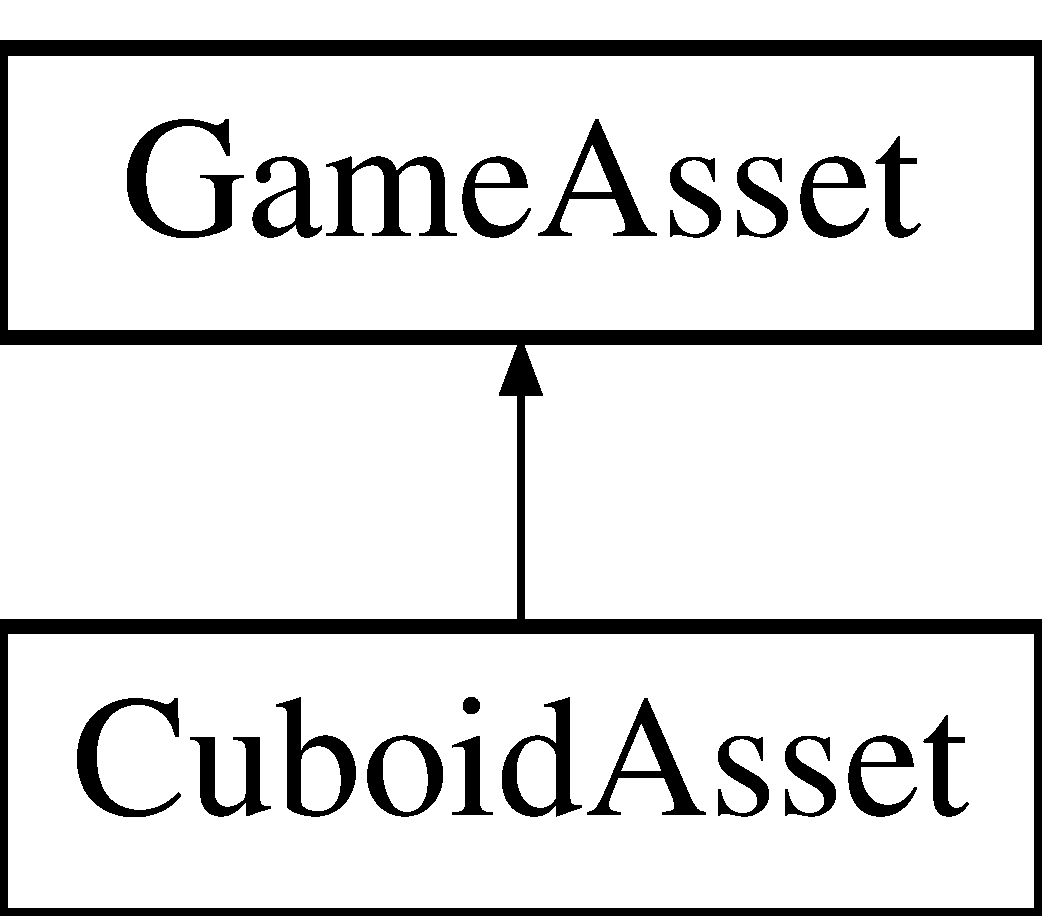
\includegraphics[height=2.000000cm]{classCuboidAsset}
\end{center}
\end{figure}
\subsection*{Public Member Functions}
\begin{DoxyCompactItemize}
\item 
\hyperlink{classCuboidAsset_a05c45a76a82b779f130b0b5828d791c2}{Cuboid\-Asset} (float x, float y, float z, float s\-X, float s\-Y, float s\-Z)
\begin{DoxyCompactList}\small\item\em Constructor Method. \end{DoxyCompactList}\item 
\hyperlink{classCuboidAsset_a9cd02d7fe04750239b9ef2245340c3c6}{Cuboid\-Asset} (float x, float y, float z, float s\-X, float s\-Y, float s\-Z, const string \&v\-\_\-shader, const string \&f\-\_\-shader)
\begin{DoxyCompactList}\small\item\em Constructor Method with shaders. \end{DoxyCompactList}\item 
virtual void \hyperlink{classCuboidAsset_a840b611da0e48bafef023ff98d97cf5b}{update} ()
\begin{DoxyCompactList}\small\item\em Update Method. \end{DoxyCompactList}\item 
virtual void \hyperlink{classCuboidAsset_adf627dc1cad3cfe5a039d829b4ad2c32}{draw} ()
\begin{DoxyCompactList}\small\item\em Draw Method. \end{DoxyCompactList}\end{DoxyCompactItemize}
\subsection*{Additional Inherited Members}


\subsection{Detailed Description}
\hyperlink{classCuboidAsset}{Cuboid\-Asset} Class. 

This class is designed to draw cuboids. 

Definition at line 18 of file Cuboid\-Asset.\-h.



\subsection{Constructor \& Destructor Documentation}
\hypertarget{classCuboidAsset_a05c45a76a82b779f130b0b5828d791c2}{\index{Cuboid\-Asset@{Cuboid\-Asset}!Cuboid\-Asset@{Cuboid\-Asset}}
\index{Cuboid\-Asset@{Cuboid\-Asset}!CuboidAsset@{Cuboid\-Asset}}
\subsubsection[{Cuboid\-Asset}]{\setlength{\rightskip}{0pt plus 5cm}Cuboid\-Asset\-::\-Cuboid\-Asset (
\begin{DoxyParamCaption}
\item[{float}]{x, }
\item[{float}]{y, }
\item[{float}]{z, }
\item[{float}]{s\-X, }
\item[{float}]{s\-Y, }
\item[{float}]{s\-Z}
\end{DoxyParamCaption}
)}}\label{classCuboidAsset_a05c45a76a82b779f130b0b5828d791c2}


Constructor Method. 

x, y, z = Coords, s\-X, s\-Y, s\-Z = dimensions 

Definition at line 11 of file Cuboid\-Asset.\-cpp.

\hypertarget{classCuboidAsset_a9cd02d7fe04750239b9ef2245340c3c6}{\index{Cuboid\-Asset@{Cuboid\-Asset}!Cuboid\-Asset@{Cuboid\-Asset}}
\index{Cuboid\-Asset@{Cuboid\-Asset}!CuboidAsset@{Cuboid\-Asset}}
\subsubsection[{Cuboid\-Asset}]{\setlength{\rightskip}{0pt plus 5cm}Cuboid\-Asset\-::\-Cuboid\-Asset (
\begin{DoxyParamCaption}
\item[{float}]{x, }
\item[{float}]{y, }
\item[{float}]{z, }
\item[{float}]{s\-X, }
\item[{float}]{s\-Y, }
\item[{float}]{s\-Z, }
\item[{const string \&}]{v\-\_\-shader, }
\item[{const string \&}]{f\-\_\-shader}
\end{DoxyParamCaption}
)}}\label{classCuboidAsset_a9cd02d7fe04750239b9ef2245340c3c6}


Constructor Method with shaders. 

Two extra parameters to customize shaders, vertex then fragment shader. 

Definition at line 23 of file Cuboid\-Asset.\-cpp.



\subsection{Member Function Documentation}
\hypertarget{classCuboidAsset_adf627dc1cad3cfe5a039d829b4ad2c32}{\index{Cuboid\-Asset@{Cuboid\-Asset}!draw@{draw}}
\index{draw@{draw}!CuboidAsset@{Cuboid\-Asset}}
\subsubsection[{draw}]{\setlength{\rightskip}{0pt plus 5cm}void Cuboid\-Asset\-::draw (
\begin{DoxyParamCaption}
{}
\end{DoxyParamCaption}
)\hspace{0.3cm}{\ttfamily [virtual]}}}\label{classCuboidAsset_adf627dc1cad3cfe5a039d829b4ad2c32}


Draw Method. 

Draws this asset in a 3\-D context. 

Reimplemented from \hyperlink{classGameAsset_a2d7e18a8f1dd8ba89ed1bd14f2affeab}{Game\-Asset}.



Definition at line 41 of file Cuboid\-Asset.\-cpp.

\hypertarget{classCuboidAsset_a840b611da0e48bafef023ff98d97cf5b}{\index{Cuboid\-Asset@{Cuboid\-Asset}!update@{update}}
\index{update@{update}!CuboidAsset@{Cuboid\-Asset}}
\subsubsection[{update}]{\setlength{\rightskip}{0pt plus 5cm}void Cuboid\-Asset\-::update (
\begin{DoxyParamCaption}
{}
\end{DoxyParamCaption}
)\hspace{0.3cm}{\ttfamily [virtual]}}}\label{classCuboidAsset_a840b611da0e48bafef023ff98d97cf5b}


Update Method. 

Updates the asset using the \hyperlink{classGAPlus}{G\-A\-Plus} movement values. 

Implements \hyperlink{classGameAsset}{Game\-Asset}.



Definition at line 35 of file Cuboid\-Asset.\-cpp.



The documentation for this class was generated from the following files\-:\begin{DoxyCompactItemize}
\item 
src/Cuboid\-Asset.\-h\item 
src/Cuboid\-Asset.\-cpp\end{DoxyCompactItemize}

\hypertarget{classData}{\section{Data Class Reference}
\label{classData}\index{Data@{Data}}
}


\hyperlink{classData}{Data} Class.  




{\ttfamily \#include $<$Data.\-h$>$}

\subsection*{Public Member Functions}
\begin{DoxyCompactItemize}
\item 
\hyperlink{classData_af11f741cb7f587e2e495452a8905a22a}{Data} ()
\begin{DoxyCompactList}\small\item\em \hyperlink{classData}{Data} Constructor. \end{DoxyCompactList}\item 
vector$<$ shared\-\_\-ptr$<$ \hyperlink{classGameAsset}{Game\-Asset} $>$ $>$ $\ast$ \hyperlink{classData_aef7cc4759b24d3f63c285fa3391b8170}{get\-List} (char c)
\begin{DoxyCompactList}\small\item\em Get List. \end{DoxyCompactList}\item 
shared\-\_\-ptr$<$ \hyperlink{classGameAsset}{Game\-Asset} $>$ \hyperlink{classData_ad9a24c281213f18b24455e4c6c168ab8}{get\-Player} ()
\begin{DoxyCompactList}\small\item\em Get Player. \end{DoxyCompactList}\end{DoxyCompactItemize}


\subsection{Detailed Description}
\hyperlink{classData}{Data} Class. 

A simple class holds data shared between classes. 

Definition at line 33 of file Data.\-h.



\subsection{Constructor \& Destructor Documentation}
\hypertarget{classData_af11f741cb7f587e2e495452a8905a22a}{\index{Data@{Data}!Data@{Data}}
\index{Data@{Data}!Data@{Data}}
\subsubsection[{Data}]{\setlength{\rightskip}{0pt plus 5cm}Data\-::\-Data (
\begin{DoxyParamCaption}
{}
\end{DoxyParamCaption}
)}}\label{classData_af11f741cb7f587e2e495452a8905a22a}


\hyperlink{classData}{Data} Constructor. 

Creates data used by multiple classes. 

Definition at line 11 of file Data.\-cpp.



\subsection{Member Function Documentation}
\hypertarget{classData_aef7cc4759b24d3f63c285fa3391b8170}{\index{Data@{Data}!get\-List@{get\-List}}
\index{get\-List@{get\-List}!Data@{Data}}
\subsubsection[{get\-List}]{\setlength{\rightskip}{0pt plus 5cm}vector$<$ shared\-\_\-ptr$<$ {\bf Game\-Asset} $>$ $>$ $\ast$ Data\-::get\-List (
\begin{DoxyParamCaption}
\item[{char}]{c}
\end{DoxyParamCaption}
)}}\label{classData_aef7cc4759b24d3f63c285fa3391b8170}


Get List. 

Returns a list depending on the char given, used to share data among classes 

Definition at line 42 of file Data.\-cpp.

\hypertarget{classData_ad9a24c281213f18b24455e4c6c168ab8}{\index{Data@{Data}!get\-Player@{get\-Player}}
\index{get\-Player@{get\-Player}!Data@{Data}}
\subsubsection[{get\-Player}]{\setlength{\rightskip}{0pt plus 5cm}shared\-\_\-ptr$<$ {\bf Game\-Asset} $>$ Data\-::get\-Player (
\begin{DoxyParamCaption}
{}
\end{DoxyParamCaption}
)}}\label{classData_ad9a24c281213f18b24455e4c6c168ab8}


Get Player. 

Returns player, used to share data among classes 

Definition at line 60 of file Data.\-cpp.



The documentation for this class was generated from the following files\-:\begin{DoxyCompactItemize}
\item 
src/Data.\-h\item 
src/Data.\-cpp\end{DoxyCompactItemize}

\hypertarget{classVectormath_1_1floatInVec}{\section{Vectormath\-:\-:float\-In\-Vec Class Reference}
\label{classVectormath_1_1floatInVec}\index{Vectormath\-::float\-In\-Vec@{Vectormath\-::float\-In\-Vec}}
}
\subsection*{Public Member Functions}
\begin{DoxyCompactItemize}
\item 
\hypertarget{classVectormath_1_1floatInVec_afaa5f27e47ae2f7c1eabfc721b2619bb}{{\bfseries float\-In\-Vec} (\hyperlink{classVectormath_1_1boolInVec}{bool\-In\-Vec} vec)}\label{classVectormath_1_1floatInVec_afaa5f27e47ae2f7c1eabfc721b2619bb}

\item 
\hypertarget{classVectormath_1_1floatInVec_a2a8e60a628d7fddb74c4941d6c296f43}{{\bfseries float\-In\-Vec} (vec\-\_\-float4 vec, int slot)}\label{classVectormath_1_1floatInVec_a2a8e60a628d7fddb74c4941d6c296f43}

\item 
\hypertarget{classVectormath_1_1floatInVec_a0d9fe72973e2d8393e29bc5891fc0549}{{\bfseries float\-In\-Vec} (float scalar)}\label{classVectormath_1_1floatInVec_a0d9fe72973e2d8393e29bc5891fc0549}

\item 
\hypertarget{classVectormath_1_1floatInVec_adf55ff2bb10f7412fc5862e55ec8be48}{{\bfseries operator float} () const }\label{classVectormath_1_1floatInVec_adf55ff2bb10f7412fc5862e55ec8be48}

\item 
\hypertarget{classVectormath_1_1floatInVec_a87ad582e3358231281651152eb26db32}{vec\-\_\-float4 {\bfseries get128} () const }\label{classVectormath_1_1floatInVec_a87ad582e3358231281651152eb26db32}

\item 
\hypertarget{classVectormath_1_1floatInVec_adf90abe101b93990227e5e7ea879bdb7}{const \hyperlink{classVectormath_1_1floatInVec}{float\-In\-Vec} {\bfseries operator++} (int)}\label{classVectormath_1_1floatInVec_adf90abe101b93990227e5e7ea879bdb7}

\item 
\hypertarget{classVectormath_1_1floatInVec_a73b9b6bb31e6e833de65a797e3d45dba}{const \hyperlink{classVectormath_1_1floatInVec}{float\-In\-Vec} {\bfseries operator-\/-\/} (int)}\label{classVectormath_1_1floatInVec_a73b9b6bb31e6e833de65a797e3d45dba}

\item 
\hypertarget{classVectormath_1_1floatInVec_a8809092da8cc4515717703ce9a405621}{\hyperlink{classVectormath_1_1floatInVec}{float\-In\-Vec} \& {\bfseries operator++} ()}\label{classVectormath_1_1floatInVec_a8809092da8cc4515717703ce9a405621}

\item 
\hypertarget{classVectormath_1_1floatInVec_a20fdc0646e155d22f5783274a9f97791}{\hyperlink{classVectormath_1_1floatInVec}{float\-In\-Vec} \& {\bfseries operator-\/-\/} ()}\label{classVectormath_1_1floatInVec_a20fdc0646e155d22f5783274a9f97791}

\item 
\hypertarget{classVectormath_1_1floatInVec_a42ef073dfef0cf53448efa875ab37f8b}{const \hyperlink{classVectormath_1_1floatInVec}{float\-In\-Vec} {\bfseries operator-\/} () const }\label{classVectormath_1_1floatInVec_a42ef073dfef0cf53448efa875ab37f8b}

\item 
\hypertarget{classVectormath_1_1floatInVec_a0191faf5ff71d0b49e0974f32b046e72}{\hyperlink{classVectormath_1_1floatInVec}{float\-In\-Vec} \& {\bfseries operator=} (\hyperlink{classVectormath_1_1floatInVec}{float\-In\-Vec} vec)}\label{classVectormath_1_1floatInVec_a0191faf5ff71d0b49e0974f32b046e72}

\item 
\hypertarget{classVectormath_1_1floatInVec_a1a6fca6462f8bcefd3c4fbdb1863c53d}{\hyperlink{classVectormath_1_1floatInVec}{float\-In\-Vec} \& {\bfseries operator$\ast$=} (\hyperlink{classVectormath_1_1floatInVec}{float\-In\-Vec} vec)}\label{classVectormath_1_1floatInVec_a1a6fca6462f8bcefd3c4fbdb1863c53d}

\item 
\hypertarget{classVectormath_1_1floatInVec_a543fed1536b4477ca4115a3587056088}{\hyperlink{classVectormath_1_1floatInVec}{float\-In\-Vec} \& {\bfseries operator/=} (\hyperlink{classVectormath_1_1floatInVec}{float\-In\-Vec} vec)}\label{classVectormath_1_1floatInVec_a543fed1536b4477ca4115a3587056088}

\item 
\hypertarget{classVectormath_1_1floatInVec_a2ebfe1983f03022daeb57b471a2b04d7}{\hyperlink{classVectormath_1_1floatInVec}{float\-In\-Vec} \& {\bfseries operator+=} (\hyperlink{classVectormath_1_1floatInVec}{float\-In\-Vec} vec)}\label{classVectormath_1_1floatInVec_a2ebfe1983f03022daeb57b471a2b04d7}

\item 
\hypertarget{classVectormath_1_1floatInVec_ad81a8950bc52b4a173a48a56616dbba6}{\hyperlink{classVectormath_1_1floatInVec}{float\-In\-Vec} \& {\bfseries operator-\/=} (\hyperlink{classVectormath_1_1floatInVec}{float\-In\-Vec} vec)}\label{classVectormath_1_1floatInVec_ad81a8950bc52b4a173a48a56616dbba6}

\item 
\hypertarget{classVectormath_1_1floatInVec_afaa5f27e47ae2f7c1eabfc721b2619bb}{{\bfseries float\-In\-Vec} (\hyperlink{classVectormath_1_1boolInVec}{bool\-In\-Vec} vec)}\label{classVectormath_1_1floatInVec_afaa5f27e47ae2f7c1eabfc721b2619bb}

\item 
\hypertarget{classVectormath_1_1floatInVec_a0d9fe72973e2d8393e29bc5891fc0549}{{\bfseries float\-In\-Vec} (float scalar)}\label{classVectormath_1_1floatInVec_a0d9fe72973e2d8393e29bc5891fc0549}

\item 
\hypertarget{classVectormath_1_1floatInVec_a2f59a1d380fd3990ba8881dc75de19bf}{float {\bfseries get\-As\-Float} () const }\label{classVectormath_1_1floatInVec_a2f59a1d380fd3990ba8881dc75de19bf}

\item 
\hypertarget{classVectormath_1_1floatInVec_adf55ff2bb10f7412fc5862e55ec8be48}{{\bfseries operator float} () const }\label{classVectormath_1_1floatInVec_adf55ff2bb10f7412fc5862e55ec8be48}

\item 
\hypertarget{classVectormath_1_1floatInVec_adf90abe101b93990227e5e7ea879bdb7}{const \hyperlink{classVectormath_1_1floatInVec}{float\-In\-Vec} {\bfseries operator++} (int)}\label{classVectormath_1_1floatInVec_adf90abe101b93990227e5e7ea879bdb7}

\item 
\hypertarget{classVectormath_1_1floatInVec_a73b9b6bb31e6e833de65a797e3d45dba}{const \hyperlink{classVectormath_1_1floatInVec}{float\-In\-Vec} {\bfseries operator-\/-\/} (int)}\label{classVectormath_1_1floatInVec_a73b9b6bb31e6e833de65a797e3d45dba}

\item 
\hypertarget{classVectormath_1_1floatInVec_ad0dda37ba47182fce20c1fd703a11079}{\hyperlink{classVectormath_1_1floatInVec}{float\-In\-Vec} \& {\bfseries operator++} ()}\label{classVectormath_1_1floatInVec_ad0dda37ba47182fce20c1fd703a11079}

\item 
\hypertarget{classVectormath_1_1floatInVec_a3816c2d1da606f4f11a1c9aa6401f1f4}{\hyperlink{classVectormath_1_1floatInVec}{float\-In\-Vec} \& {\bfseries operator-\/-\/} ()}\label{classVectormath_1_1floatInVec_a3816c2d1da606f4f11a1c9aa6401f1f4}

\item 
\hypertarget{classVectormath_1_1floatInVec_a42ef073dfef0cf53448efa875ab37f8b}{const \hyperlink{classVectormath_1_1floatInVec}{float\-In\-Vec} {\bfseries operator-\/} () const }\label{classVectormath_1_1floatInVec_a42ef073dfef0cf53448efa875ab37f8b}

\item 
\hypertarget{classVectormath_1_1floatInVec_a7fd53fb7bb89b6d858a058ef44545063}{\hyperlink{classVectormath_1_1floatInVec}{float\-In\-Vec} \& {\bfseries operator=} (\hyperlink{classVectormath_1_1floatInVec}{float\-In\-Vec} vec)}\label{classVectormath_1_1floatInVec_a7fd53fb7bb89b6d858a058ef44545063}

\item 
\hypertarget{classVectormath_1_1floatInVec_a2884665205bf0ebae6204f4e96b8d2db}{\hyperlink{classVectormath_1_1floatInVec}{float\-In\-Vec} \& {\bfseries operator$\ast$=} (\hyperlink{classVectormath_1_1floatInVec}{float\-In\-Vec} vec)}\label{classVectormath_1_1floatInVec_a2884665205bf0ebae6204f4e96b8d2db}

\item 
\hypertarget{classVectormath_1_1floatInVec_ad6b2db4477b1f19631221ce9bf18e549}{\hyperlink{classVectormath_1_1floatInVec}{float\-In\-Vec} \& {\bfseries operator/=} (\hyperlink{classVectormath_1_1floatInVec}{float\-In\-Vec} vec)}\label{classVectormath_1_1floatInVec_ad6b2db4477b1f19631221ce9bf18e549}

\item 
\hypertarget{classVectormath_1_1floatInVec_ac9b3f52606ac0a721dc7fbbde0116cdd}{\hyperlink{classVectormath_1_1floatInVec}{float\-In\-Vec} \& {\bfseries operator+=} (\hyperlink{classVectormath_1_1floatInVec}{float\-In\-Vec} vec)}\label{classVectormath_1_1floatInVec_ac9b3f52606ac0a721dc7fbbde0116cdd}

\item 
\hypertarget{classVectormath_1_1floatInVec_ad73a4378c77f7d4e60a486ecd6b0440b}{\hyperlink{classVectormath_1_1floatInVec}{float\-In\-Vec} \& {\bfseries operator-\/=} (\hyperlink{classVectormath_1_1floatInVec}{float\-In\-Vec} vec)}\label{classVectormath_1_1floatInVec_ad73a4378c77f7d4e60a486ecd6b0440b}

\item 
\hypertarget{classVectormath_1_1floatInVec_afaa5f27e47ae2f7c1eabfc721b2619bb}{{\bfseries float\-In\-Vec} (\hyperlink{classVectormath_1_1boolInVec}{bool\-In\-Vec} vec)}\label{classVectormath_1_1floatInVec_afaa5f27e47ae2f7c1eabfc721b2619bb}

\item 
\hypertarget{classVectormath_1_1floatInVec_a2a8e60a628d7fddb74c4941d6c296f43}{{\bfseries float\-In\-Vec} (vec\-\_\-float4 vec, int slot)}\label{classVectormath_1_1floatInVec_a2a8e60a628d7fddb74c4941d6c296f43}

\item 
\hypertarget{classVectormath_1_1floatInVec_a0d9fe72973e2d8393e29bc5891fc0549}{{\bfseries float\-In\-Vec} (float scalar)}\label{classVectormath_1_1floatInVec_a0d9fe72973e2d8393e29bc5891fc0549}

\item 
\hypertarget{classVectormath_1_1floatInVec_adf55ff2bb10f7412fc5862e55ec8be48}{{\bfseries operator float} () const }\label{classVectormath_1_1floatInVec_adf55ff2bb10f7412fc5862e55ec8be48}

\item 
\hypertarget{classVectormath_1_1floatInVec_a8ddc6f070be18010b5beb6a4e6127ea8}{vec\-\_\-float4 {\bfseries get128} () const }\label{classVectormath_1_1floatInVec_a8ddc6f070be18010b5beb6a4e6127ea8}

\item 
\hypertarget{classVectormath_1_1floatInVec_adf90abe101b93990227e5e7ea879bdb7}{const \hyperlink{classVectormath_1_1floatInVec}{float\-In\-Vec} {\bfseries operator++} (int)}\label{classVectormath_1_1floatInVec_adf90abe101b93990227e5e7ea879bdb7}

\item 
\hypertarget{classVectormath_1_1floatInVec_a73b9b6bb31e6e833de65a797e3d45dba}{const \hyperlink{classVectormath_1_1floatInVec}{float\-In\-Vec} {\bfseries operator-\/-\/} (int)}\label{classVectormath_1_1floatInVec_a73b9b6bb31e6e833de65a797e3d45dba}

\item 
\hypertarget{classVectormath_1_1floatInVec_ad0dda37ba47182fce20c1fd703a11079}{\hyperlink{classVectormath_1_1floatInVec}{float\-In\-Vec} \& {\bfseries operator++} ()}\label{classVectormath_1_1floatInVec_ad0dda37ba47182fce20c1fd703a11079}

\item 
\hypertarget{classVectormath_1_1floatInVec_a3816c2d1da606f4f11a1c9aa6401f1f4}{\hyperlink{classVectormath_1_1floatInVec}{float\-In\-Vec} \& {\bfseries operator-\/-\/} ()}\label{classVectormath_1_1floatInVec_a3816c2d1da606f4f11a1c9aa6401f1f4}

\item 
\hypertarget{classVectormath_1_1floatInVec_a42ef073dfef0cf53448efa875ab37f8b}{const \hyperlink{classVectormath_1_1floatInVec}{float\-In\-Vec} {\bfseries operator-\/} () const }\label{classVectormath_1_1floatInVec_a42ef073dfef0cf53448efa875ab37f8b}

\item 
\hypertarget{classVectormath_1_1floatInVec_a7fd53fb7bb89b6d858a058ef44545063}{\hyperlink{classVectormath_1_1floatInVec}{float\-In\-Vec} \& {\bfseries operator=} (\hyperlink{classVectormath_1_1floatInVec}{float\-In\-Vec} vec)}\label{classVectormath_1_1floatInVec_a7fd53fb7bb89b6d858a058ef44545063}

\item 
\hypertarget{classVectormath_1_1floatInVec_a2884665205bf0ebae6204f4e96b8d2db}{\hyperlink{classVectormath_1_1floatInVec}{float\-In\-Vec} \& {\bfseries operator$\ast$=} (\hyperlink{classVectormath_1_1floatInVec}{float\-In\-Vec} vec)}\label{classVectormath_1_1floatInVec_a2884665205bf0ebae6204f4e96b8d2db}

\item 
\hypertarget{classVectormath_1_1floatInVec_ad6b2db4477b1f19631221ce9bf18e549}{\hyperlink{classVectormath_1_1floatInVec}{float\-In\-Vec} \& {\bfseries operator/=} (\hyperlink{classVectormath_1_1floatInVec}{float\-In\-Vec} vec)}\label{classVectormath_1_1floatInVec_ad6b2db4477b1f19631221ce9bf18e549}

\item 
\hypertarget{classVectormath_1_1floatInVec_ac9b3f52606ac0a721dc7fbbde0116cdd}{\hyperlink{classVectormath_1_1floatInVec}{float\-In\-Vec} \& {\bfseries operator+=} (\hyperlink{classVectormath_1_1floatInVec}{float\-In\-Vec} vec)}\label{classVectormath_1_1floatInVec_ac9b3f52606ac0a721dc7fbbde0116cdd}

\item 
\hypertarget{classVectormath_1_1floatInVec_ad73a4378c77f7d4e60a486ecd6b0440b}{\hyperlink{classVectormath_1_1floatInVec}{float\-In\-Vec} \& {\bfseries operator-\/=} (\hyperlink{classVectormath_1_1floatInVec}{float\-In\-Vec} vec)}\label{classVectormath_1_1floatInVec_ad73a4378c77f7d4e60a486ecd6b0440b}

\item 
\hypertarget{classVectormath_1_1floatInVec_a9b5b7f66bc5a374b007861e995c61546}{{\bfseries float\-In\-Vec} (\-\_\-\-\_\-m128 vec)}\label{classVectormath_1_1floatInVec_a9b5b7f66bc5a374b007861e995c61546}

\item 
\hypertarget{classVectormath_1_1floatInVec_a8ca388d2a9425ef6b4407918da809779}{{\bfseries float\-In\-Vec} (const \hyperlink{classVectormath_1_1boolInVec}{bool\-In\-Vec} \&vec)}\label{classVectormath_1_1floatInVec_a8ca388d2a9425ef6b4407918da809779}

\item 
\hypertarget{classVectormath_1_1floatInVec_a540f58821d53d7f530470b650b559d6c}{{\bfseries float\-In\-Vec} (\-\_\-\-\_\-m128 vec, int slot)}\label{classVectormath_1_1floatInVec_a540f58821d53d7f530470b650b559d6c}

\item 
\hypertarget{classVectormath_1_1floatInVec_a0d9fe72973e2d8393e29bc5891fc0549}{{\bfseries float\-In\-Vec} (float scalar)}\label{classVectormath_1_1floatInVec_a0d9fe72973e2d8393e29bc5891fc0549}

\item 
\hypertarget{classVectormath_1_1floatInVec_adf55ff2bb10f7412fc5862e55ec8be48}{{\bfseries operator float} () const }\label{classVectormath_1_1floatInVec_adf55ff2bb10f7412fc5862e55ec8be48}

\item 
\hypertarget{classVectormath_1_1floatInVec_a87ad582e3358231281651152eb26db32}{\-\_\-\-\_\-m128 {\bfseries get128} () const }\label{classVectormath_1_1floatInVec_a87ad582e3358231281651152eb26db32}

\item 
\hypertarget{classVectormath_1_1floatInVec_adf90abe101b93990227e5e7ea879bdb7}{const \hyperlink{classVectormath_1_1floatInVec}{float\-In\-Vec} {\bfseries operator++} (int)}\label{classVectormath_1_1floatInVec_adf90abe101b93990227e5e7ea879bdb7}

\item 
\hypertarget{classVectormath_1_1floatInVec_a73b9b6bb31e6e833de65a797e3d45dba}{const \hyperlink{classVectormath_1_1floatInVec}{float\-In\-Vec} {\bfseries operator-\/-\/} (int)}\label{classVectormath_1_1floatInVec_a73b9b6bb31e6e833de65a797e3d45dba}

\item 
\hypertarget{classVectormath_1_1floatInVec_ad0dda37ba47182fce20c1fd703a11079}{\hyperlink{classVectormath_1_1floatInVec}{float\-In\-Vec} \& {\bfseries operator++} ()}\label{classVectormath_1_1floatInVec_ad0dda37ba47182fce20c1fd703a11079}

\item 
\hypertarget{classVectormath_1_1floatInVec_a3816c2d1da606f4f11a1c9aa6401f1f4}{\hyperlink{classVectormath_1_1floatInVec}{float\-In\-Vec} \& {\bfseries operator-\/-\/} ()}\label{classVectormath_1_1floatInVec_a3816c2d1da606f4f11a1c9aa6401f1f4}

\item 
\hypertarget{classVectormath_1_1floatInVec_a42ef073dfef0cf53448efa875ab37f8b}{const \hyperlink{classVectormath_1_1floatInVec}{float\-In\-Vec} {\bfseries operator-\/} () const }\label{classVectormath_1_1floatInVec_a42ef073dfef0cf53448efa875ab37f8b}

\item 
\hypertarget{classVectormath_1_1floatInVec_ac83a598aef0c03baad69e4e8df68d0e6}{\hyperlink{classVectormath_1_1floatInVec}{float\-In\-Vec} \& {\bfseries operator=} (const \hyperlink{classVectormath_1_1floatInVec}{float\-In\-Vec} \&vec)}\label{classVectormath_1_1floatInVec_ac83a598aef0c03baad69e4e8df68d0e6}

\item 
\hypertarget{classVectormath_1_1floatInVec_aa760d0df8666316bf96c714cc0fa974a}{\hyperlink{classVectormath_1_1floatInVec}{float\-In\-Vec} \& {\bfseries operator$\ast$=} (const \hyperlink{classVectormath_1_1floatInVec}{float\-In\-Vec} \&vec)}\label{classVectormath_1_1floatInVec_aa760d0df8666316bf96c714cc0fa974a}

\item 
\hypertarget{classVectormath_1_1floatInVec_aeadf90e7eeffc761a74f63bb2b9845b3}{\hyperlink{classVectormath_1_1floatInVec}{float\-In\-Vec} \& {\bfseries operator/=} (const \hyperlink{classVectormath_1_1floatInVec}{float\-In\-Vec} \&vec)}\label{classVectormath_1_1floatInVec_aeadf90e7eeffc761a74f63bb2b9845b3}

\item 
\hypertarget{classVectormath_1_1floatInVec_aa2ad1f3734be46010e4d04561de4189e}{\hyperlink{classVectormath_1_1floatInVec}{float\-In\-Vec} \& {\bfseries operator+=} (const \hyperlink{classVectormath_1_1floatInVec}{float\-In\-Vec} \&vec)}\label{classVectormath_1_1floatInVec_aa2ad1f3734be46010e4d04561de4189e}

\item 
\hypertarget{classVectormath_1_1floatInVec_a89738930b594c679be9033a2b67d6004}{\hyperlink{classVectormath_1_1floatInVec}{float\-In\-Vec} \& {\bfseries operator-\/=} (const \hyperlink{classVectormath_1_1floatInVec}{float\-In\-Vec} \&vec)}\label{classVectormath_1_1floatInVec_a89738930b594c679be9033a2b67d6004}

\end{DoxyCompactItemize}
\subsection*{Friends}
\begin{DoxyCompactItemize}
\item 
\hypertarget{classVectormath_1_1floatInVec_a9f97436600c786a7cf4a6bbd847d48af}{const \hyperlink{classVectormath_1_1floatInVec}{float\-In\-Vec} {\bfseries operator$\ast$} (\hyperlink{classVectormath_1_1floatInVec}{float\-In\-Vec} vec0, \hyperlink{classVectormath_1_1floatInVec}{float\-In\-Vec} vec1)}\label{classVectormath_1_1floatInVec_a9f97436600c786a7cf4a6bbd847d48af}

\item 
\hypertarget{classVectormath_1_1floatInVec_a45425f8c4a644ad4e68a0f695f63feee}{const \hyperlink{classVectormath_1_1floatInVec}{float\-In\-Vec} {\bfseries operator/} (\hyperlink{classVectormath_1_1floatInVec}{float\-In\-Vec} vec0, \hyperlink{classVectormath_1_1floatInVec}{float\-In\-Vec} vec1)}\label{classVectormath_1_1floatInVec_a45425f8c4a644ad4e68a0f695f63feee}

\item 
\hypertarget{classVectormath_1_1floatInVec_af55f7e5d4004c1c539e4f6ec92ba0c62}{const \hyperlink{classVectormath_1_1floatInVec}{float\-In\-Vec} {\bfseries operator+} (\hyperlink{classVectormath_1_1floatInVec}{float\-In\-Vec} vec0, \hyperlink{classVectormath_1_1floatInVec}{float\-In\-Vec} vec1)}\label{classVectormath_1_1floatInVec_af55f7e5d4004c1c539e4f6ec92ba0c62}

\item 
\hypertarget{classVectormath_1_1floatInVec_aedff0079a93c6938cf4771e19091e6e3}{const \hyperlink{classVectormath_1_1floatInVec}{float\-In\-Vec} {\bfseries operator-\/} (\hyperlink{classVectormath_1_1floatInVec}{float\-In\-Vec} vec0, \hyperlink{classVectormath_1_1floatInVec}{float\-In\-Vec} vec1)}\label{classVectormath_1_1floatInVec_aedff0079a93c6938cf4771e19091e6e3}

\item 
\hypertarget{classVectormath_1_1floatInVec_a2861ac5749cb945d8d27afa055c9db17}{const \hyperlink{classVectormath_1_1floatInVec}{float\-In\-Vec} {\bfseries select} (\hyperlink{classVectormath_1_1floatInVec}{float\-In\-Vec} vec0, \hyperlink{classVectormath_1_1floatInVec}{float\-In\-Vec} vec1, \hyperlink{classVectormath_1_1boolInVec}{bool\-In\-Vec} select\-\_\-vec1)}\label{classVectormath_1_1floatInVec_a2861ac5749cb945d8d27afa055c9db17}

\item 
\hypertarget{classVectormath_1_1floatInVec_a9f97436600c786a7cf4a6bbd847d48af}{const \hyperlink{classVectormath_1_1floatInVec}{float\-In\-Vec} {\bfseries operator$\ast$} (\hyperlink{classVectormath_1_1floatInVec}{float\-In\-Vec} vec0, \hyperlink{classVectormath_1_1floatInVec}{float\-In\-Vec} vec1)}\label{classVectormath_1_1floatInVec_a9f97436600c786a7cf4a6bbd847d48af}

\item 
\hypertarget{classVectormath_1_1floatInVec_a45425f8c4a644ad4e68a0f695f63feee}{const \hyperlink{classVectormath_1_1floatInVec}{float\-In\-Vec} {\bfseries operator/} (\hyperlink{classVectormath_1_1floatInVec}{float\-In\-Vec} vec0, \hyperlink{classVectormath_1_1floatInVec}{float\-In\-Vec} vec1)}\label{classVectormath_1_1floatInVec_a45425f8c4a644ad4e68a0f695f63feee}

\item 
\hypertarget{classVectormath_1_1floatInVec_af55f7e5d4004c1c539e4f6ec92ba0c62}{const \hyperlink{classVectormath_1_1floatInVec}{float\-In\-Vec} {\bfseries operator+} (\hyperlink{classVectormath_1_1floatInVec}{float\-In\-Vec} vec0, \hyperlink{classVectormath_1_1floatInVec}{float\-In\-Vec} vec1)}\label{classVectormath_1_1floatInVec_af55f7e5d4004c1c539e4f6ec92ba0c62}

\item 
\hypertarget{classVectormath_1_1floatInVec_aedff0079a93c6938cf4771e19091e6e3}{const \hyperlink{classVectormath_1_1floatInVec}{float\-In\-Vec} {\bfseries operator-\/} (\hyperlink{classVectormath_1_1floatInVec}{float\-In\-Vec} vec0, \hyperlink{classVectormath_1_1floatInVec}{float\-In\-Vec} vec1)}\label{classVectormath_1_1floatInVec_aedff0079a93c6938cf4771e19091e6e3}

\item 
\hypertarget{classVectormath_1_1floatInVec_a2861ac5749cb945d8d27afa055c9db17}{const \hyperlink{classVectormath_1_1floatInVec}{float\-In\-Vec} {\bfseries select} (\hyperlink{classVectormath_1_1floatInVec}{float\-In\-Vec} vec0, \hyperlink{classVectormath_1_1floatInVec}{float\-In\-Vec} vec1, \hyperlink{classVectormath_1_1boolInVec}{bool\-In\-Vec} select\-\_\-vec1)}\label{classVectormath_1_1floatInVec_a2861ac5749cb945d8d27afa055c9db17}

\item 
\hypertarget{classVectormath_1_1floatInVec_a3245c1626b36c482334db45b5b86721c}{const \hyperlink{classVectormath_1_1floatInVec}{float\-In\-Vec} {\bfseries operator$\ast$} (const \hyperlink{classVectormath_1_1floatInVec}{float\-In\-Vec} \&vec0, const \hyperlink{classVectormath_1_1floatInVec}{float\-In\-Vec} \&vec1)}\label{classVectormath_1_1floatInVec_a3245c1626b36c482334db45b5b86721c}

\item 
\hypertarget{classVectormath_1_1floatInVec_a45e96ad304260d908bfc6d2b51b210d2}{const \hyperlink{classVectormath_1_1floatInVec}{float\-In\-Vec} {\bfseries operator/} (const \hyperlink{classVectormath_1_1floatInVec}{float\-In\-Vec} \&vec0, const \hyperlink{classVectormath_1_1floatInVec}{float\-In\-Vec} \&vec1)}\label{classVectormath_1_1floatInVec_a45e96ad304260d908bfc6d2b51b210d2}

\item 
\hypertarget{classVectormath_1_1floatInVec_a9e67ab843002e647fa7bb2caed760bdc}{const \hyperlink{classVectormath_1_1floatInVec}{float\-In\-Vec} {\bfseries operator+} (const \hyperlink{classVectormath_1_1floatInVec}{float\-In\-Vec} \&vec0, const \hyperlink{classVectormath_1_1floatInVec}{float\-In\-Vec} \&vec1)}\label{classVectormath_1_1floatInVec_a9e67ab843002e647fa7bb2caed760bdc}

\item 
\hypertarget{classVectormath_1_1floatInVec_ac6c858483e69952c29682d153854fbe2}{const \hyperlink{classVectormath_1_1floatInVec}{float\-In\-Vec} {\bfseries operator-\/} (const \hyperlink{classVectormath_1_1floatInVec}{float\-In\-Vec} \&vec0, const \hyperlink{classVectormath_1_1floatInVec}{float\-In\-Vec} \&vec1)}\label{classVectormath_1_1floatInVec_ac6c858483e69952c29682d153854fbe2}

\item 
\hypertarget{classVectormath_1_1floatInVec_a2970b847bee6dc51a58e7b308ab866c0}{const \hyperlink{classVectormath_1_1floatInVec}{float\-In\-Vec} {\bfseries select} (const \hyperlink{classVectormath_1_1floatInVec}{float\-In\-Vec} \&vec0, const \hyperlink{classVectormath_1_1floatInVec}{float\-In\-Vec} \&vec1, \hyperlink{classVectormath_1_1boolInVec}{bool\-In\-Vec} select\-\_\-vec1)}\label{classVectormath_1_1floatInVec_a2970b847bee6dc51a58e7b308ab866c0}

\end{DoxyCompactItemize}


\subsection{Detailed Description}


Definition at line 48 of file float\-In\-Vec.\-h.



The documentation for this class was generated from the following file\-:\begin{DoxyCompactItemize}
\item 
src/include/vectormath/ppu/cpp/float\-In\-Vec.\-h\end{DoxyCompactItemize}

\hypertarget{classGameAsset}{\section{Game\-Asset Class Reference}
\label{classGameAsset}\index{Game\-Asset@{Game\-Asset}}
}


\hyperlink{classGameAsset}{Game\-Asset} Class.  




{\ttfamily \#include $<$Game\-Asset.\-h$>$}

Inheritance diagram for Game\-Asset\-:\begin{figure}[H]
\begin{center}
\leavevmode
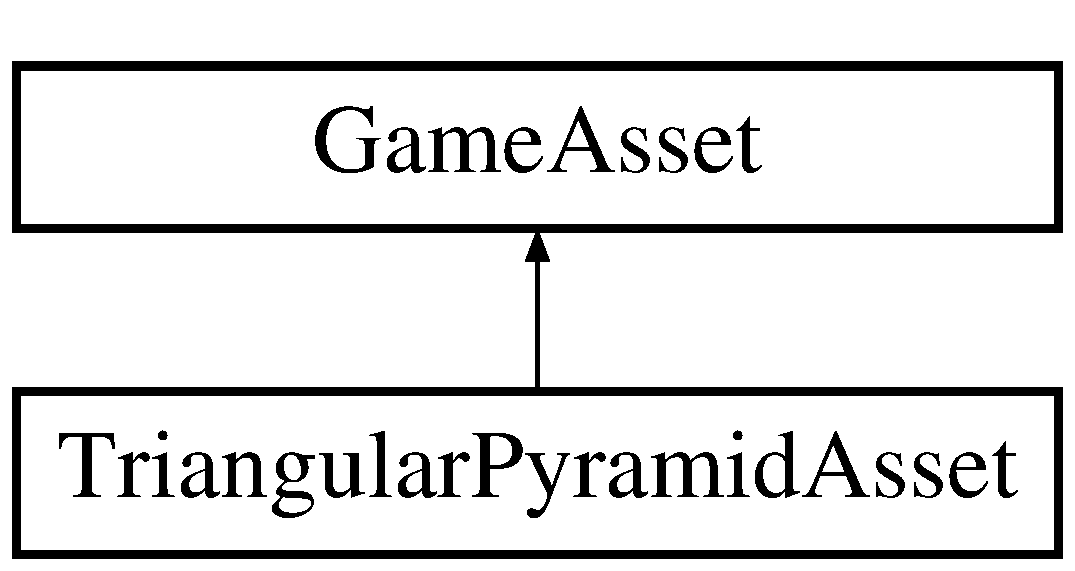
\includegraphics[height=2.000000cm]{classGameAsset}
\end{center}
\end{figure}
\subsection*{Public Member Functions}
\begin{DoxyCompactItemize}
\item 
\hypertarget{classGameAsset_ac6d2340f41dd95e71892327dae4e1585}{{\bfseries Game\-Asset} (const string \&v\-\_\-shader, const string \&f\-\_\-shader)}\label{classGameAsset_ac6d2340f41dd95e71892327dae4e1585}

\item 
bool \hyperlink{classGameAsset_a612793ce2a354d2f8839a779d0ca2227}{collides\-With} (\hyperlink{classGameAsset}{Game\-Asset} \&a)
\begin{DoxyCompactList}\small\item\em Collision method. \end{DoxyCompactList}\item 
\hypertarget{classGameAsset_a2d7e18a8f1dd8ba89ed1bd14f2affeab}{virtual void {\bfseries draw} ()}\label{classGameAsset_a2d7e18a8f1dd8ba89ed1bd14f2affeab}

\item 
\hypertarget{classGameAsset_a42688ec8f02e201eaaa01e74a112083f}{virtual void {\bfseries update} ()=0}\label{classGameAsset_a42688ec8f02e201eaaa01e74a112083f}

\end{DoxyCompactItemize}
\subsection*{Protected Member Functions}
\begin{DoxyCompactItemize}
\item 
int \hyperlink{classGameAsset_aa26d85233ece476d599adf90074e9568}{make\-\_\-resources} ()
\begin{DoxyCompactList}\small\item\em Create shaders \& buffers method. \end{DoxyCompactList}\item 
G\-Lchar $\ast$ \hyperlink{classGameAsset_a08c617aafc70dcba441f53260f1bb09f}{shader\-\_\-file\-\_\-contents} (const string \&filename, G\-Lint $\ast$length)
\begin{DoxyCompactList}\small\item\em Shader file reader. \end{DoxyCompactList}\item 
G\-Luint \hyperlink{classGameAsset_adfe27369433f07092b08f24b0feedfc9}{make\-\_\-buffer} (G\-Lenum target, const void $\ast$buffer\-\_\-data, G\-Lsizei buffer\-\_\-size)
\begin{DoxyCompactList}\small\item\em Create Buffers method. \end{DoxyCompactList}\item 
G\-Luint \hyperlink{classGameAsset_ac728e885b52c93c3e4976a339de54545}{make\-\_\-shader} (G\-Lenum type, const char $\ast$filename)
\begin{DoxyCompactList}\small\item\em Create Shaders method. \end{DoxyCompactList}\item 
G\-Luint \hyperlink{classGameAsset_a9d9574a21cf6b52f7a825879ca50b19d}{make\-\_\-program} (G\-Luint vertex\-\_\-shader, G\-Luint fragment\-\_\-shader)
\begin{DoxyCompactList}\small\item\em Create program method. \end{DoxyCompactList}\item 
vector$<$ \hyperlink{classModelTriangle}{Model\-Triangle} $>$ \hyperlink{classGameAsset_aad7eeea6e2a9544fd2b2fff522cca56b}{get\-Triangles} ()
\end{DoxyCompactItemize}
\subsection*{Protected Attributes}
\begin{DoxyCompactItemize}
\item 
\hypertarget{classGameAsset_a1a1d227eba2765b025f9f453700c2359}{G\-Luint {\bfseries vertex\-\_\-buffer}}\label{classGameAsset_a1a1d227eba2765b025f9f453700c2359}

\item 
\hypertarget{classGameAsset_a5e005ff1d4280e73f67446353e78fe43}{G\-Luint {\bfseries element\-\_\-buffer}}\label{classGameAsset_a5e005ff1d4280e73f67446353e78fe43}

\item 
\hypertarget{classGameAsset_aba95de2870f78ac21568bbf9dd7e2b40}{G\-Luint {\bfseries vertex\-\_\-shader}}\label{classGameAsset_aba95de2870f78ac21568bbf9dd7e2b40}

\item 
\hypertarget{classGameAsset_ab62d9e2547537bd89eeae057a402a895}{G\-Luint {\bfseries fragment\-\_\-shader}}\label{classGameAsset_ab62d9e2547537bd89eeae057a402a895}

\item 
\hypertarget{classGameAsset_a239f03ead1a34924e76d6f875216404b}{G\-Luint {\bfseries program}}\label{classGameAsset_a239f03ead1a34924e76d6f875216404b}

\item 
\hypertarget{classGameAsset_ad8c8198dcc470301e8f5eae8dc8506bb}{G\-Lint {\bfseries position\-\_\-attrib}}\label{classGameAsset_ad8c8198dcc470301e8f5eae8dc8506bb}

\item 
\hypertarget{classGameAsset_a402a20952864f5992ee3c42a9d7e977f}{G\-Lint {\bfseries camera\-\_\-uniform}}\label{classGameAsset_a402a20952864f5992ee3c42a9d7e977f}

\item 
\hypertarget{classGameAsset_aa39bb998856e0065e1ead5f192fb995c}{G\-Lint {\bfseries model\-\_\-uniform}}\label{classGameAsset_aa39bb998856e0065e1ead5f192fb995c}

\item 
\hypertarget{classGameAsset_ae1d682ecf84d9cd3f91a8c870acf2777}{G\-Lfloat $\ast$ {\bfseries g\-\_\-vertex\-\_\-buffer\-\_\-data}}\label{classGameAsset_ae1d682ecf84d9cd3f91a8c870acf2777}

\item 
\hypertarget{classGameAsset_ab859393c9158c8bda39cd100475fee25}{G\-Lushort $\ast$ {\bfseries g\-\_\-element\-\_\-buffer\-\_\-data}}\label{classGameAsset_ab859393c9158c8bda39cd100475fee25}

\item 
\hypertarget{classGameAsset_a3e8d7dc58d3d4efafbbce1536b78dbc7}{int {\bfseries num\-\_\-vertices}}\label{classGameAsset_a3e8d7dc58d3d4efafbbce1536b78dbc7}

\item 
\hypertarget{classGameAsset_aae4d864335c2eca685cc86602881cd18}{int {\bfseries num\-\_\-triangles}}\label{classGameAsset_aae4d864335c2eca685cc86602881cd18}

\item 
\hypertarget{classGameAsset_a3444a096fed505b1740bedc95e2cfa6c}{shared\-\_\-ptr$<$ \hyperlink{classBoundingBox}{Bounding\-Box} $>$ {\bfseries bbox}}\label{classGameAsset_a3444a096fed505b1740bedc95e2cfa6c}

\end{DoxyCompactItemize}


\subsection{Detailed Description}
\hyperlink{classGameAsset}{Game\-Asset} Class. 

The super class of all other objects in the game, containing vertex \& fragment shaders and the objects model. 

Definition at line 33 of file Game\-Asset.\-h.



\subsection{Member Function Documentation}
\hypertarget{classGameAsset_a612793ce2a354d2f8839a779d0ca2227}{\index{Game\-Asset@{Game\-Asset}!collides\-With@{collides\-With}}
\index{collides\-With@{collides\-With}!GameAsset@{Game\-Asset}}
\subsubsection[{collides\-With}]{\setlength{\rightskip}{0pt plus 5cm}bool Game\-Asset\-::collides\-With (
\begin{DoxyParamCaption}
\item[{{\bf Game\-Asset} \&}]{a}
\end{DoxyParamCaption}
)}}\label{classGameAsset_a612793ce2a354d2f8839a779d0ca2227}


Collision method. 

Method to detect if this asset collides with given asset. 

Definition at line 31 of file Game\-Asset.\-cpp.

\hypertarget{classGameAsset_aad7eeea6e2a9544fd2b2fff522cca56b}{\index{Game\-Asset@{Game\-Asset}!get\-Triangles@{get\-Triangles}}
\index{get\-Triangles@{get\-Triangles}!GameAsset@{Game\-Asset}}
\subsubsection[{get\-Triangles}]{\setlength{\rightskip}{0pt plus 5cm}vector$<$ {\bf Model\-Triangle} $>$ Game\-Asset\-::get\-Triangles (
\begin{DoxyParamCaption}
{}
\end{DoxyParamCaption}
)\hspace{0.3cm}{\ttfamily [protected]}}}\label{classGameAsset_aad7eeea6e2a9544fd2b2fff522cca56b}
Returns this model as a list of \hyperlink{classModelTriangle}{Model\-Triangle} 

Definition at line 42 of file Game\-Asset.\-cpp.

\hypertarget{classGameAsset_adfe27369433f07092b08f24b0feedfc9}{\index{Game\-Asset@{Game\-Asset}!make\-\_\-buffer@{make\-\_\-buffer}}
\index{make\-\_\-buffer@{make\-\_\-buffer}!GameAsset@{Game\-Asset}}
\subsubsection[{make\-\_\-buffer}]{\setlength{\rightskip}{0pt plus 5cm}G\-Luint Game\-Asset\-::make\-\_\-buffer (
\begin{DoxyParamCaption}
\item[{G\-Lenum}]{target, }
\item[{const void $\ast$}]{buffer\-\_\-data, }
\item[{G\-Lsizei}]{buffer\-\_\-size}
\end{DoxyParamCaption}
)\hspace{0.3cm}{\ttfamily [protected]}}}\label{classGameAsset_adfe27369433f07092b08f24b0feedfc9}


Create Buffers method. 

Creates this assets buffers. 

Definition at line 133 of file Game\-Asset.\-cpp.

\hypertarget{classGameAsset_a9d9574a21cf6b52f7a825879ca50b19d}{\index{Game\-Asset@{Game\-Asset}!make\-\_\-program@{make\-\_\-program}}
\index{make\-\_\-program@{make\-\_\-program}!GameAsset@{Game\-Asset}}
\subsubsection[{make\-\_\-program}]{\setlength{\rightskip}{0pt plus 5cm}G\-Luint Game\-Asset\-::make\-\_\-program (
\begin{DoxyParamCaption}
\item[{G\-Luint}]{vertex\-\_\-shader, }
\item[{G\-Luint}]{fragment\-\_\-shader}
\end{DoxyParamCaption}
)\hspace{0.3cm}{\ttfamily [protected]}}}\label{classGameAsset_a9d9574a21cf6b52f7a825879ca50b19d}


Create program method. 

Creates this assets shader program. 

Definition at line 169 of file Game\-Asset.\-cpp.

\hypertarget{classGameAsset_aa26d85233ece476d599adf90074e9568}{\index{Game\-Asset@{Game\-Asset}!make\-\_\-resources@{make\-\_\-resources}}
\index{make\-\_\-resources@{make\-\_\-resources}!GameAsset@{Game\-Asset}}
\subsubsection[{make\-\_\-resources}]{\setlength{\rightskip}{0pt plus 5cm}int Game\-Asset\-::make\-\_\-resources (
\begin{DoxyParamCaption}
\item[{void}]{}
\end{DoxyParamCaption}
)\hspace{0.3cm}{\ttfamily [protected]}}}\label{classGameAsset_aa26d85233ece476d599adf90074e9568}


Create shaders \& buffers method. 

Creates this assets buffers, shaders and shader program. 

Definition at line 191 of file Game\-Asset.\-cpp.

\hypertarget{classGameAsset_ac728e885b52c93c3e4976a339de54545}{\index{Game\-Asset@{Game\-Asset}!make\-\_\-shader@{make\-\_\-shader}}
\index{make\-\_\-shader@{make\-\_\-shader}!GameAsset@{Game\-Asset}}
\subsubsection[{make\-\_\-shader}]{\setlength{\rightskip}{0pt plus 5cm}G\-Luint Game\-Asset\-::make\-\_\-shader (
\begin{DoxyParamCaption}
\item[{G\-Lenum}]{type, }
\item[{const char $\ast$}]{filename}
\end{DoxyParamCaption}
)\hspace{0.3cm}{\ttfamily [protected]}}}\label{classGameAsset_ac728e885b52c93c3e4976a339de54545}


Create Shaders method. 

Creates this assets shaders. 

Definition at line 145 of file Game\-Asset.\-cpp.

\hypertarget{classGameAsset_a08c617aafc70dcba441f53260f1bb09f}{\index{Game\-Asset@{Game\-Asset}!shader\-\_\-file\-\_\-contents@{shader\-\_\-file\-\_\-contents}}
\index{shader\-\_\-file\-\_\-contents@{shader\-\_\-file\-\_\-contents}!GameAsset@{Game\-Asset}}
\subsubsection[{shader\-\_\-file\-\_\-contents}]{\setlength{\rightskip}{0pt plus 5cm}G\-Lchar $\ast$ Game\-Asset\-::shader\-\_\-file\-\_\-contents (
\begin{DoxyParamCaption}
\item[{const string \&}]{filename, }
\item[{G\-Lint $\ast$}]{length}
\end{DoxyParamCaption}
)\hspace{0.3cm}{\ttfamily [protected]}}}\label{classGameAsset_a08c617aafc70dcba441f53260f1bb09f}


Shader file reader. 

Reads this \hyperlink{classGameAsset}{Game\-Asset}'s shader file and returns it. 

Definition at line 113 of file Game\-Asset.\-cpp.



The documentation for this class was generated from the following files\-:\begin{DoxyCompactItemize}
\item 
src/Game\-Asset.\-h\item 
src/Game\-Asset.\-cpp\end{DoxyCompactItemize}

\hypertarget{classGAPlus}{\section{G\-A\-Plus Class Reference}
\label{classGAPlus}\index{G\-A\-Plus@{G\-A\-Plus}}
}


\hyperlink{classGAPlus}{G\-A\-Plus} Class.  




{\ttfamily \#include $<$G\-A\-Plus.\-h$>$}

\subsection*{Public Member Functions}
\begin{DoxyCompactItemize}
\item 
\hyperlink{classGAPlus_ac6953ed1932735d5f916b24f1298f3ab}{G\-A\-Plus} (char t, vector$<$ Global\-::\-Force $>$ f)
\begin{DoxyCompactList}\small\item\em \hyperlink{classGAPlus}{G\-A\-Plus} Constructor. \end{DoxyCompactList}\item 
char \hyperlink{classGAPlus_aadfbeaa73754fc498542ee0faa879912}{get\-Ty} ()
\begin{DoxyCompactList}\small\item\em Get type method. \end{DoxyCompactList}\item 
vector$<$ Global\-::\-Force $>$ \hyperlink{classGAPlus_a424b0920996c254e25f95f03d553d7d7}{get\-For} ()
\begin{DoxyCompactList}\small\item\em Get list of forces method. \end{DoxyCompactList}\item 
\hypertarget{classGAPlus_a9743f921683de213d9f66abffd6970c3}{float \hyperlink{classGAPlus_a9743f921683de213d9f66abffd6970c3}{get\-Mov\-X} ()}\label{classGAPlus_a9743f921683de213d9f66abffd6970c3}

\begin{DoxyCompactList}\small\item\em Get movement value along X axis. \end{DoxyCompactList}\item 
\hypertarget{classGAPlus_acffcea1f1028eec9ed47c71c6830ef87}{float \hyperlink{classGAPlus_acffcea1f1028eec9ed47c71c6830ef87}{get\-Mov\-Y} ()}\label{classGAPlus_acffcea1f1028eec9ed47c71c6830ef87}

\begin{DoxyCompactList}\small\item\em Get movement value along Y axis. \end{DoxyCompactList}\item 
\hypertarget{classGAPlus_abaa790b578ae3f93c341f1d3badaa5ed}{float \hyperlink{classGAPlus_abaa790b578ae3f93c341f1d3badaa5ed}{get\-Mov\-Z} ()}\label{classGAPlus_abaa790b578ae3f93c341f1d3badaa5ed}

\begin{DoxyCompactList}\small\item\em Get movement value along Z axis. \end{DoxyCompactList}\item 
\hypertarget{classGAPlus_a2e58d254ad8a5b25d9de8fdaab3ab4b7}{void \hyperlink{classGAPlus_a2e58d254ad8a5b25d9de8fdaab3ab4b7}{set\-Mov\-X} (float x)}\label{classGAPlus_a2e58d254ad8a5b25d9de8fdaab3ab4b7}

\begin{DoxyCompactList}\small\item\em Set movement value along X axis. \end{DoxyCompactList}\item 
\hypertarget{classGAPlus_a742b62c8fb4cbc9644c396226448f7e8}{void \hyperlink{classGAPlus_a742b62c8fb4cbc9644c396226448f7e8}{set\-Mov\-Y} (float y)}\label{classGAPlus_a742b62c8fb4cbc9644c396226448f7e8}

\begin{DoxyCompactList}\small\item\em Set movement value along Y axis. \end{DoxyCompactList}\item 
\hypertarget{classGAPlus_aec3ef9cf7ffbaeeee2c9837e5734a880}{void \hyperlink{classGAPlus_aec3ef9cf7ffbaeeee2c9837e5734a880}{set\-Mov\-Z} (float z)}\label{classGAPlus_aec3ef9cf7ffbaeeee2c9837e5734a880}

\begin{DoxyCompactList}\small\item\em Set movement value along Z axis. \end{DoxyCompactList}\end{DoxyCompactItemize}


\subsection{Detailed Description}
\hyperlink{classGAPlus}{G\-A\-Plus} Class. 

Holds more information on a \hyperlink{classGameAsset}{Game\-Asset}. 

Definition at line 20 of file G\-A\-Plus.\-h.



\subsection{Constructor \& Destructor Documentation}
\hypertarget{classGAPlus_ac6953ed1932735d5f916b24f1298f3ab}{\index{G\-A\-Plus@{G\-A\-Plus}!G\-A\-Plus@{G\-A\-Plus}}
\index{G\-A\-Plus@{G\-A\-Plus}!GAPlus@{G\-A\-Plus}}
\subsubsection[{G\-A\-Plus}]{\setlength{\rightskip}{0pt plus 5cm}G\-A\-Plus\-::\-G\-A\-Plus (
\begin{DoxyParamCaption}
\item[{char}]{t, }
\item[{vector$<$ Global\-::\-Force $>$}]{f}
\end{DoxyParamCaption}
)}}\label{classGAPlus_ac6953ed1932735d5f916b24f1298f3ab}


\hyperlink{classGAPlus}{G\-A\-Plus} Constructor. 

Requires a char, which represents what the \hyperlink{classGameAsset}{Game\-Asset} is, and a list of forces this Asset is subject to. 

Definition at line 10 of file G\-A\-Plus.\-cpp.



\subsection{Member Function Documentation}
\hypertarget{classGAPlus_a424b0920996c254e25f95f03d553d7d7}{\index{G\-A\-Plus@{G\-A\-Plus}!get\-For@{get\-For}}
\index{get\-For@{get\-For}!GAPlus@{G\-A\-Plus}}
\subsubsection[{get\-For}]{\setlength{\rightskip}{0pt plus 5cm}vector$<$ Global\-::\-Force $>$ G\-A\-Plus\-::get\-For (
\begin{DoxyParamCaption}
{}
\end{DoxyParamCaption}
)}}\label{classGAPlus_a424b0920996c254e25f95f03d553d7d7}


Get list of forces method. 

List of forces this Asset is subject to. 

Definition at line 28 of file G\-A\-Plus.\-cpp.

\hypertarget{classGAPlus_aadfbeaa73754fc498542ee0faa879912}{\index{G\-A\-Plus@{G\-A\-Plus}!get\-Ty@{get\-Ty}}
\index{get\-Ty@{get\-Ty}!GAPlus@{G\-A\-Plus}}
\subsubsection[{get\-Ty}]{\setlength{\rightskip}{0pt plus 5cm}char G\-A\-Plus\-::get\-Ty (
\begin{DoxyParamCaption}
{}
\end{DoxyParamCaption}
)}}\label{classGAPlus_aadfbeaa73754fc498542ee0faa879912}


Get type method. 

Type = char 

Definition at line 23 of file G\-A\-Plus.\-cpp.



The documentation for this class was generated from the following files\-:\begin{DoxyCompactItemize}
\item 
src/G\-A\-Plus.\-h\item 
src/G\-A\-Plus.\-cpp\end{DoxyCompactItemize}

\hypertarget{classGlobal}{\section{Global Class Reference}
\label{classGlobal}\index{Global@{Global}}
}


\hyperlink{classGlobal}{Global} Header.  




{\ttfamily \#include $<$Global.\-h$>$}

\subsection*{Public Types}
\begin{DoxyCompactItemize}
\item 
enum {\bfseries Force} \{ {\bfseries G\-R\-A\-V}, 
{\bfseries C\-O\-L\-S}, 
{\bfseries S\-T\-A\-T}, 
{\bfseries D\-Y\-N\-A}
 \}
\end{DoxyCompactItemize}


\subsection{Detailed Description}
\hyperlink{classGlobal}{Global} Header. 

Holds parameters relating to physics etc. 

Definition at line 16 of file Global.\-h.



The documentation for this class was generated from the following file\-:\begin{DoxyCompactItemize}
\item 
src/Global.\-h\end{DoxyCompactItemize}

\hypertarget{classIInterpolator}{\section{I\-Interpolator Class Reference}
\label{classIInterpolator}\index{I\-Interpolator@{I\-Interpolator}}
}
Inheritance diagram for I\-Interpolator\-:\begin{figure}[H]
\begin{center}
\leavevmode
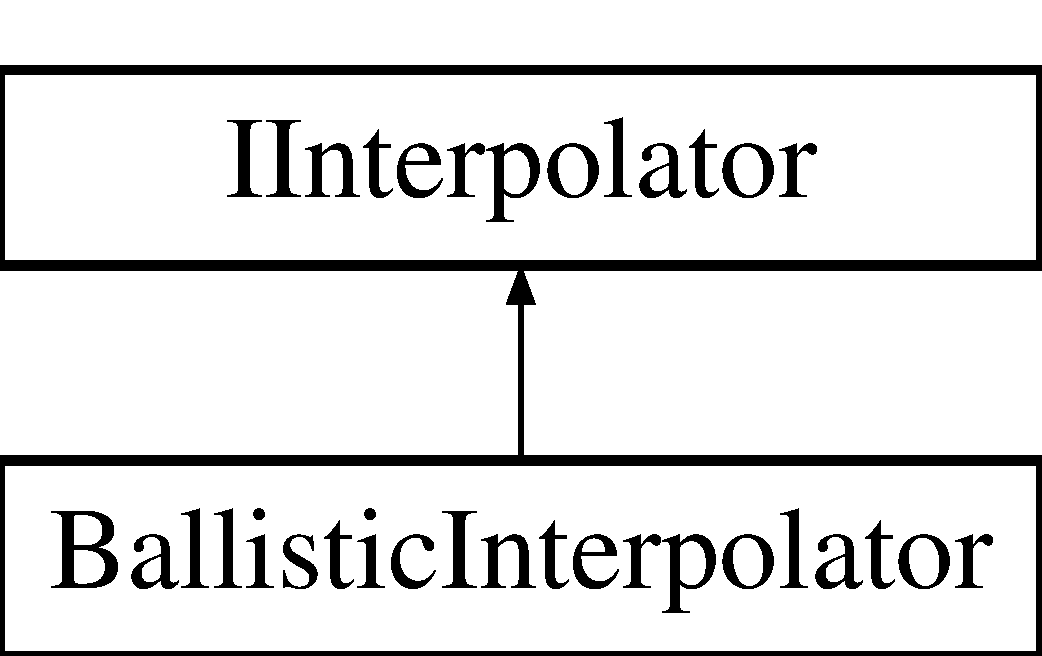
\includegraphics[height=2.000000cm]{classIInterpolator}
\end{center}
\end{figure}
\subsection*{Public Member Functions}
\begin{DoxyCompactItemize}
\item 
\hypertarget{classIInterpolator_ae808dd40665d235fa0abfadf0aa8d0d1}{virtual \hyperlink{classVectormath_1_1Aos_1_1Vector3}{Vector3} {\bfseries update} ()=0}\label{classIInterpolator_ae808dd40665d235fa0abfadf0aa8d0d1}

\end{DoxyCompactItemize}


\subsection{Detailed Description}


Definition at line 15 of file I\-Interpolator.\-h.



The documentation for this class was generated from the following file\-:\begin{DoxyCompactItemize}
\item 
src/I\-Interpolator.\-h\end{DoxyCompactItemize}

\hypertarget{classLevelLoader}{\section{Level\-Loader Class Reference}
\label{classLevelLoader}\index{Level\-Loader@{Level\-Loader}}
}


Level Class.  




{\ttfamily \#include $<$Level\-Loader.\-h$>$}

\subsection*{Public Member Functions}
\begin{DoxyCompactItemize}
\item 
vector$<$ shared\-\_\-ptr$<$ \hyperlink{classGameAsset}{Game\-Asset} $>$ $>$ \hyperlink{classLevelLoader_aa6c896057092099df7ec221628daaa56}{get\-Level} (int)
\begin{DoxyCompactList}\small\item\em Get level method. \end{DoxyCompactList}\end{DoxyCompactItemize}


\subsection{Detailed Description}
Level Class. 

A simple class that reads a .txt file and produces creates a vector of Game\-Assets based on it. 

Definition at line 18 of file Level\-Loader.\-h.



\subsection{Member Function Documentation}
\hypertarget{classLevelLoader_aa6c896057092099df7ec221628daaa56}{\index{Level\-Loader@{Level\-Loader}!get\-Level@{get\-Level}}
\index{get\-Level@{get\-Level}!LevelLoader@{Level\-Loader}}
\subsubsection[{get\-Level}]{\setlength{\rightskip}{0pt plus 5cm}vector$<$ shared\-\_\-ptr$<$ {\bf Game\-Asset} $>$ $>$ Level\-Loader\-::get\-Level (
\begin{DoxyParamCaption}
\item[{int}]{i}
\end{DoxyParamCaption}
)}}\label{classLevelLoader_aa6c896057092099df7ec221628daaa56}


Get level method. 

Sends an integer which acts as the level name, returning a vector of \hyperlink{classGameAsset}{Game\-Asset}. 

Definition at line 3 of file Level\-Loader.\-cpp.



The documentation for this class was generated from the following files\-:\begin{DoxyCompactItemize}
\item 
src/Level\-Loader.\-h\item 
src/Level\-Loader.\-cpp\end{DoxyCompactItemize}

\hypertarget{classLoop}{\section{Loop Class Reference}
\label{classLoop}\index{Loop@{Loop}}
}


\hyperlink{classLoop}{Loop} Class.  




{\ttfamily \#include $<$Loop.\-h$>$}

\subsection*{Public Member Functions}
\begin{DoxyCompactItemize}
\item 
\hyperlink{classLoop_ab9ef9206b3b9472f958ff288bd6e5167}{Loop} (S\-D\-L\-\_\-\-Window $\ast$temp\-Window)
\begin{DoxyCompactList}\small\item\em \hyperlink{classLoop}{Loop} Constructor. \end{DoxyCompactList}\item 
\hypertarget{classLoop_adc4809c26a1fd3fefe4592fa1b42222a}{void \hyperlink{classLoop_adc4809c26a1fd3fefe4592fa1b42222a}{game\-Loop} ()}\label{classLoop_adc4809c26a1fd3fefe4592fa1b42222a}

\begin{DoxyCompactList}\small\item\em Main loop Method. \end{DoxyCompactList}\end{DoxyCompactItemize}


\subsection{Detailed Description}
\hyperlink{classLoop}{Loop} Class. 

A simple class that loops the game world calling other classes etc. 

Definition at line 36 of file Loop.\-h.



\subsection{Constructor \& Destructor Documentation}
\hypertarget{classLoop_ab9ef9206b3b9472f958ff288bd6e5167}{\index{Loop@{Loop}!Loop@{Loop}}
\index{Loop@{Loop}!Loop@{Loop}}
\subsubsection[{Loop}]{\setlength{\rightskip}{0pt plus 5cm}Loop\-::\-Loop (
\begin{DoxyParamCaption}
\item[{S\-D\-L\-\_\-\-Window $\ast$}]{temp\-Window}
\end{DoxyParamCaption}
)}}\label{classLoop_ab9ef9206b3b9472f958ff288bd6e5167}


\hyperlink{classLoop}{Loop} Constructor. 

Initialises world to be looped sending window created in Main 

Definition at line 25 of file Loop.\-cpp.



The documentation for this class was generated from the following files\-:\begin{DoxyCompactItemize}
\item 
src/Loop.\-h\item 
src/Loop.\-cpp\end{DoxyCompactItemize}

\hypertarget{classVectormath_1_1Aos_1_1Matrix3}{\section{Vectormath\-:\-:Aos\-:\-:Matrix3 Class Reference}
\label{classVectormath_1_1Aos_1_1Matrix3}\index{Vectormath\-::\-Aos\-::\-Matrix3@{Vectormath\-::\-Aos\-::\-Matrix3}}
}
\subsection*{Public Member Functions}
\begin{DoxyCompactItemize}
\item 
\hypertarget{classVectormath_1_1Aos_1_1Matrix3_a3e073b4d8297328a7d63fa80657752df}{{\bfseries Matrix3} (const \hyperlink{classVectormath_1_1Aos_1_1Matrix3}{Matrix3} \&mat)}\label{classVectormath_1_1Aos_1_1Matrix3_a3e073b4d8297328a7d63fa80657752df}

\item 
\hypertarget{classVectormath_1_1Aos_1_1Matrix3_a279da8a93caa0cd39f8845543898dd23}{{\bfseries Matrix3} (\hyperlink{classVectormath_1_1Aos_1_1Vector3}{Vector3} col0, \hyperlink{classVectormath_1_1Aos_1_1Vector3}{Vector3} col1, \hyperlink{classVectormath_1_1Aos_1_1Vector3}{Vector3} col2)}\label{classVectormath_1_1Aos_1_1Matrix3_a279da8a93caa0cd39f8845543898dd23}

\item 
\hypertarget{classVectormath_1_1Aos_1_1Matrix3_ae3472b21c6c5f1796aac1a3b68739190}{{\bfseries Matrix3} (\hyperlink{classVectormath_1_1Aos_1_1Quat}{Quat} unit\-Quat)}\label{classVectormath_1_1Aos_1_1Matrix3_ae3472b21c6c5f1796aac1a3b68739190}

\item 
\hypertarget{classVectormath_1_1Aos_1_1Matrix3_ab789a362d913ac070001534adb906e0c}{{\bfseries Matrix3} (float scalar)}\label{classVectormath_1_1Aos_1_1Matrix3_ab789a362d913ac070001534adb906e0c}

\item 
\hypertarget{classVectormath_1_1Aos_1_1Matrix3_ac3ed42719d9b026f3ea025cb88169695}{{\bfseries Matrix3} (\hyperlink{classVectormath_1_1floatInVec}{float\-In\-Vec} scalar)}\label{classVectormath_1_1Aos_1_1Matrix3_ac3ed42719d9b026f3ea025cb88169695}

\item 
\hypertarget{classVectormath_1_1Aos_1_1Matrix3_ac0cca76c1d4f774f76902efa0bb6bd76}{\hyperlink{classVectormath_1_1Aos_1_1Matrix3}{Matrix3} \& {\bfseries operator=} (const \hyperlink{classVectormath_1_1Aos_1_1Matrix3}{Matrix3} \&mat)}\label{classVectormath_1_1Aos_1_1Matrix3_ac0cca76c1d4f774f76902efa0bb6bd76}

\item 
\hypertarget{classVectormath_1_1Aos_1_1Matrix3_a50ef15e610024fb06b78f76cd2a2440e}{\hyperlink{classVectormath_1_1Aos_1_1Matrix3}{Matrix3} \& {\bfseries set\-Col0} (\hyperlink{classVectormath_1_1Aos_1_1Vector3}{Vector3} col0)}\label{classVectormath_1_1Aos_1_1Matrix3_a50ef15e610024fb06b78f76cd2a2440e}

\item 
\hypertarget{classVectormath_1_1Aos_1_1Matrix3_ab3c3ade9b8b53579fe605f65a709e89b}{\hyperlink{classVectormath_1_1Aos_1_1Matrix3}{Matrix3} \& {\bfseries set\-Col1} (\hyperlink{classVectormath_1_1Aos_1_1Vector3}{Vector3} col1)}\label{classVectormath_1_1Aos_1_1Matrix3_ab3c3ade9b8b53579fe605f65a709e89b}

\item 
\hypertarget{classVectormath_1_1Aos_1_1Matrix3_ab563e9c01994d51f11774674e5ffbb46}{\hyperlink{classVectormath_1_1Aos_1_1Matrix3}{Matrix3} \& {\bfseries set\-Col2} (\hyperlink{classVectormath_1_1Aos_1_1Vector3}{Vector3} col2)}\label{classVectormath_1_1Aos_1_1Matrix3_ab563e9c01994d51f11774674e5ffbb46}

\item 
\hypertarget{classVectormath_1_1Aos_1_1Matrix3_ad8e1efab5f4ca2d2049f2898992c7b59}{const \hyperlink{classVectormath_1_1Aos_1_1Vector3}{Vector3} {\bfseries get\-Col0} () const }\label{classVectormath_1_1Aos_1_1Matrix3_ad8e1efab5f4ca2d2049f2898992c7b59}

\item 
\hypertarget{classVectormath_1_1Aos_1_1Matrix3_a2c9c0d7059cb6ea36ea1a10a064d883b}{const \hyperlink{classVectormath_1_1Aos_1_1Vector3}{Vector3} {\bfseries get\-Col1} () const }\label{classVectormath_1_1Aos_1_1Matrix3_a2c9c0d7059cb6ea36ea1a10a064d883b}

\item 
\hypertarget{classVectormath_1_1Aos_1_1Matrix3_a74aaf602f55ad6797c27fcfde59f06bd}{const \hyperlink{classVectormath_1_1Aos_1_1Vector3}{Vector3} {\bfseries get\-Col2} () const }\label{classVectormath_1_1Aos_1_1Matrix3_a74aaf602f55ad6797c27fcfde59f06bd}

\item 
\hypertarget{classVectormath_1_1Aos_1_1Matrix3_a9718c8866ce1b7e2b39cefbf2d72dfa9}{\hyperlink{classVectormath_1_1Aos_1_1Matrix3}{Matrix3} \& {\bfseries set\-Col} (int col, \hyperlink{classVectormath_1_1Aos_1_1Vector3}{Vector3} vec)}\label{classVectormath_1_1Aos_1_1Matrix3_a9718c8866ce1b7e2b39cefbf2d72dfa9}

\item 
\hypertarget{classVectormath_1_1Aos_1_1Matrix3_a96df632d4777bea8f9ce9dfc3bbb89f5}{\hyperlink{classVectormath_1_1Aos_1_1Matrix3}{Matrix3} \& {\bfseries set\-Row} (int row, \hyperlink{classVectormath_1_1Aos_1_1Vector3}{Vector3} vec)}\label{classVectormath_1_1Aos_1_1Matrix3_a96df632d4777bea8f9ce9dfc3bbb89f5}

\item 
\hypertarget{classVectormath_1_1Aos_1_1Matrix3_af99478271b4f24368fa0181602039fa0}{const \hyperlink{classVectormath_1_1Aos_1_1Vector3}{Vector3} {\bfseries get\-Col} (int col) const }\label{classVectormath_1_1Aos_1_1Matrix3_af99478271b4f24368fa0181602039fa0}

\item 
\hypertarget{classVectormath_1_1Aos_1_1Matrix3_ae5fb935a0847e76728c1d50c924ec533}{const \hyperlink{classVectormath_1_1Aos_1_1Vector3}{Vector3} {\bfseries get\-Row} (int row) const }\label{classVectormath_1_1Aos_1_1Matrix3_ae5fb935a0847e76728c1d50c924ec533}

\item 
\hypertarget{classVectormath_1_1Aos_1_1Matrix3_a0f31da424c1971810de23146f00c4162}{\hyperlink{classVectormath_1_1Aos_1_1Vector3}{Vector3} \& {\bfseries operator\mbox{[}$\,$\mbox{]}} (int col)}\label{classVectormath_1_1Aos_1_1Matrix3_a0f31da424c1971810de23146f00c4162}

\item 
\hypertarget{classVectormath_1_1Aos_1_1Matrix3_aae9b49cc796d80afaccbc35aa2a525e5}{const \hyperlink{classVectormath_1_1Aos_1_1Vector3}{Vector3} {\bfseries operator\mbox{[}$\,$\mbox{]}} (int col) const }\label{classVectormath_1_1Aos_1_1Matrix3_aae9b49cc796d80afaccbc35aa2a525e5}

\item 
\hypertarget{classVectormath_1_1Aos_1_1Matrix3_a15e7e2f35f6b3373304630762f749153}{\hyperlink{classVectormath_1_1Aos_1_1Matrix3}{Matrix3} \& {\bfseries set\-Elem} (int col, int row, float val)}\label{classVectormath_1_1Aos_1_1Matrix3_a15e7e2f35f6b3373304630762f749153}

\item 
\hypertarget{classVectormath_1_1Aos_1_1Matrix3_aca529c327fd294cb02995445257ccd7d}{\hyperlink{classVectormath_1_1Aos_1_1Matrix3}{Matrix3} \& {\bfseries set\-Elem} (int col, int row, \hyperlink{classVectormath_1_1floatInVec}{float\-In\-Vec} val)}\label{classVectormath_1_1Aos_1_1Matrix3_aca529c327fd294cb02995445257ccd7d}

\item 
\hypertarget{classVectormath_1_1Aos_1_1Matrix3_ae086fc63661174df257f91373702a036}{const \hyperlink{classVectormath_1_1floatInVec}{float\-In\-Vec} {\bfseries get\-Elem} (int col, int row) const }\label{classVectormath_1_1Aos_1_1Matrix3_ae086fc63661174df257f91373702a036}

\item 
\hypertarget{classVectormath_1_1Aos_1_1Matrix3_a97dd5cb8fcb16e375eddc486be298a49}{const \hyperlink{classVectormath_1_1Aos_1_1Matrix3}{Matrix3} {\bfseries operator+} (const \hyperlink{classVectormath_1_1Aos_1_1Matrix3}{Matrix3} \&mat) const }\label{classVectormath_1_1Aos_1_1Matrix3_a97dd5cb8fcb16e375eddc486be298a49}

\item 
\hypertarget{classVectormath_1_1Aos_1_1Matrix3_abf21280f20e4192c7dba3824b6a4e2cc}{const \hyperlink{classVectormath_1_1Aos_1_1Matrix3}{Matrix3} {\bfseries operator-\/} (const \hyperlink{classVectormath_1_1Aos_1_1Matrix3}{Matrix3} \&mat) const }\label{classVectormath_1_1Aos_1_1Matrix3_abf21280f20e4192c7dba3824b6a4e2cc}

\item 
\hypertarget{classVectormath_1_1Aos_1_1Matrix3_ab3dd83421ca0570267dbd5ea3f55a288}{const \hyperlink{classVectormath_1_1Aos_1_1Matrix3}{Matrix3} {\bfseries operator-\/} () const }\label{classVectormath_1_1Aos_1_1Matrix3_ab3dd83421ca0570267dbd5ea3f55a288}

\item 
\hypertarget{classVectormath_1_1Aos_1_1Matrix3_a3ead19fc46afc8d1212a357705b7321a}{const \hyperlink{classVectormath_1_1Aos_1_1Matrix3}{Matrix3} {\bfseries operator$\ast$} (float scalar) const }\label{classVectormath_1_1Aos_1_1Matrix3_a3ead19fc46afc8d1212a357705b7321a}

\item 
\hypertarget{classVectormath_1_1Aos_1_1Matrix3_a2279bfe34cba4c55b91f709b70f97f80}{const \hyperlink{classVectormath_1_1Aos_1_1Matrix3}{Matrix3} {\bfseries operator$\ast$} (\hyperlink{classVectormath_1_1floatInVec}{float\-In\-Vec} scalar) const }\label{classVectormath_1_1Aos_1_1Matrix3_a2279bfe34cba4c55b91f709b70f97f80}

\item 
\hypertarget{classVectormath_1_1Aos_1_1Matrix3_a13f0a1e4db8008823fd01ee2407e4dab}{const \hyperlink{classVectormath_1_1Aos_1_1Vector3}{Vector3} {\bfseries operator$\ast$} (\hyperlink{classVectormath_1_1Aos_1_1Vector3}{Vector3} vec) const }\label{classVectormath_1_1Aos_1_1Matrix3_a13f0a1e4db8008823fd01ee2407e4dab}

\item 
\hypertarget{classVectormath_1_1Aos_1_1Matrix3_aacb897d2c06b1eaafe68fc147909d1d1}{const \hyperlink{classVectormath_1_1Aos_1_1Matrix3}{Matrix3} {\bfseries operator$\ast$} (const \hyperlink{classVectormath_1_1Aos_1_1Matrix3}{Matrix3} \&mat) const }\label{classVectormath_1_1Aos_1_1Matrix3_aacb897d2c06b1eaafe68fc147909d1d1}

\item 
\hypertarget{classVectormath_1_1Aos_1_1Matrix3_a9a0638e4795da0e30b1c334793648201}{\hyperlink{classVectormath_1_1Aos_1_1Matrix3}{Matrix3} \& {\bfseries operator+=} (const \hyperlink{classVectormath_1_1Aos_1_1Matrix3}{Matrix3} \&mat)}\label{classVectormath_1_1Aos_1_1Matrix3_a9a0638e4795da0e30b1c334793648201}

\item 
\hypertarget{classVectormath_1_1Aos_1_1Matrix3_ac3edd9953ac35b9d435624f409b2ca66}{\hyperlink{classVectormath_1_1Aos_1_1Matrix3}{Matrix3} \& {\bfseries operator-\/=} (const \hyperlink{classVectormath_1_1Aos_1_1Matrix3}{Matrix3} \&mat)}\label{classVectormath_1_1Aos_1_1Matrix3_ac3edd9953ac35b9d435624f409b2ca66}

\item 
\hypertarget{classVectormath_1_1Aos_1_1Matrix3_a4a09fe7dbbd8f95d0c22ed27a60b77ea}{\hyperlink{classVectormath_1_1Aos_1_1Matrix3}{Matrix3} \& {\bfseries operator$\ast$=} (float scalar)}\label{classVectormath_1_1Aos_1_1Matrix3_a4a09fe7dbbd8f95d0c22ed27a60b77ea}

\item 
\hypertarget{classVectormath_1_1Aos_1_1Matrix3_a02e50b29f6bdcc8c5e8f53b23ae79494}{\hyperlink{classVectormath_1_1Aos_1_1Matrix3}{Matrix3} \& {\bfseries operator$\ast$=} (\hyperlink{classVectormath_1_1floatInVec}{float\-In\-Vec} scalar)}\label{classVectormath_1_1Aos_1_1Matrix3_a02e50b29f6bdcc8c5e8f53b23ae79494}

\item 
\hypertarget{classVectormath_1_1Aos_1_1Matrix3_a87488f974b0fad884071127e99165dc5}{\hyperlink{classVectormath_1_1Aos_1_1Matrix3}{Matrix3} \& {\bfseries operator$\ast$=} (const \hyperlink{classVectormath_1_1Aos_1_1Matrix3}{Matrix3} \&mat)}\label{classVectormath_1_1Aos_1_1Matrix3_a87488f974b0fad884071127e99165dc5}

\item 
\hypertarget{classVectormath_1_1Aos_1_1Matrix3_ad40ce9469c3eb035e45955e197fb2f69}{{\bfseries Matrix3} (const \hyperlink{classVectormath_1_1Aos_1_1Matrix3}{Matrix3} \&mat)}\label{classVectormath_1_1Aos_1_1Matrix3_ad40ce9469c3eb035e45955e197fb2f69}

\item 
\hypertarget{classVectormath_1_1Aos_1_1Matrix3_a4f5ff411513382c646cd1aa71111c4bc}{{\bfseries Matrix3} (const \hyperlink{classVectormath_1_1Aos_1_1Vector3}{Vector3} \&col0, const \hyperlink{classVectormath_1_1Aos_1_1Vector3}{Vector3} \&col1, const \hyperlink{classVectormath_1_1Aos_1_1Vector3}{Vector3} \&col2)}\label{classVectormath_1_1Aos_1_1Matrix3_a4f5ff411513382c646cd1aa71111c4bc}

\item 
\hypertarget{classVectormath_1_1Aos_1_1Matrix3_a3fa42f848e2674bcadf512fe13a015ea}{{\bfseries Matrix3} (const \hyperlink{classVectormath_1_1Aos_1_1Quat}{Quat} \&unit\-Quat)}\label{classVectormath_1_1Aos_1_1Matrix3_a3fa42f848e2674bcadf512fe13a015ea}

\item 
\hypertarget{classVectormath_1_1Aos_1_1Matrix3_a54a63372a7b411ef3133f73dc070c13c}{{\bfseries Matrix3} (float scalar)}\label{classVectormath_1_1Aos_1_1Matrix3_a54a63372a7b411ef3133f73dc070c13c}

\item 
\hypertarget{classVectormath_1_1Aos_1_1Matrix3_a48694136c5c7033cf4f8b49fb16e06a3}{\hyperlink{classVectormath_1_1Aos_1_1Matrix3}{Matrix3} \& {\bfseries operator=} (const \hyperlink{classVectormath_1_1Aos_1_1Matrix3}{Matrix3} \&mat)}\label{classVectormath_1_1Aos_1_1Matrix3_a48694136c5c7033cf4f8b49fb16e06a3}

\item 
\hypertarget{classVectormath_1_1Aos_1_1Matrix3_ab0f90bd4c442bae35457dd1d81e29e89}{\hyperlink{classVectormath_1_1Aos_1_1Matrix3}{Matrix3} \& {\bfseries set\-Col0} (const \hyperlink{classVectormath_1_1Aos_1_1Vector3}{Vector3} \&col0)}\label{classVectormath_1_1Aos_1_1Matrix3_ab0f90bd4c442bae35457dd1d81e29e89}

\item 
\hypertarget{classVectormath_1_1Aos_1_1Matrix3_a9062d71b93ec9357666f04a3283b62c3}{\hyperlink{classVectormath_1_1Aos_1_1Matrix3}{Matrix3} \& {\bfseries set\-Col1} (const \hyperlink{classVectormath_1_1Aos_1_1Vector3}{Vector3} \&col1)}\label{classVectormath_1_1Aos_1_1Matrix3_a9062d71b93ec9357666f04a3283b62c3}

\item 
\hypertarget{classVectormath_1_1Aos_1_1Matrix3_a9911d669a2653b7db8aab82ad81be991}{\hyperlink{classVectormath_1_1Aos_1_1Matrix3}{Matrix3} \& {\bfseries set\-Col2} (const \hyperlink{classVectormath_1_1Aos_1_1Vector3}{Vector3} \&col2)}\label{classVectormath_1_1Aos_1_1Matrix3_a9911d669a2653b7db8aab82ad81be991}

\item 
\hypertarget{classVectormath_1_1Aos_1_1Matrix3_a9210bff3e38bc93a54e727e2a12b9e18}{const \hyperlink{classVectormath_1_1Aos_1_1Vector3}{Vector3} {\bfseries get\-Col0} () const }\label{classVectormath_1_1Aos_1_1Matrix3_a9210bff3e38bc93a54e727e2a12b9e18}

\item 
\hypertarget{classVectormath_1_1Aos_1_1Matrix3_ad26bbc279a2cdcbab29172716155dfcf}{const \hyperlink{classVectormath_1_1Aos_1_1Vector3}{Vector3} {\bfseries get\-Col1} () const }\label{classVectormath_1_1Aos_1_1Matrix3_ad26bbc279a2cdcbab29172716155dfcf}

\item 
\hypertarget{classVectormath_1_1Aos_1_1Matrix3_abe2e97ccc608b6fa920d91291f52b9f8}{const \hyperlink{classVectormath_1_1Aos_1_1Vector3}{Vector3} {\bfseries get\-Col2} () const }\label{classVectormath_1_1Aos_1_1Matrix3_abe2e97ccc608b6fa920d91291f52b9f8}

\item 
\hypertarget{classVectormath_1_1Aos_1_1Matrix3_acd8044bfd0034fb9ec354df65482ed33}{\hyperlink{classVectormath_1_1Aos_1_1Matrix3}{Matrix3} \& {\bfseries set\-Col} (int col, const \hyperlink{classVectormath_1_1Aos_1_1Vector3}{Vector3} \&vec)}\label{classVectormath_1_1Aos_1_1Matrix3_acd8044bfd0034fb9ec354df65482ed33}

\item 
\hypertarget{classVectormath_1_1Aos_1_1Matrix3_a541f629224aa3f8941b16013d6c8dce0}{\hyperlink{classVectormath_1_1Aos_1_1Matrix3}{Matrix3} \& {\bfseries set\-Row} (int row, const \hyperlink{classVectormath_1_1Aos_1_1Vector3}{Vector3} \&vec)}\label{classVectormath_1_1Aos_1_1Matrix3_a541f629224aa3f8941b16013d6c8dce0}

\item 
\hypertarget{classVectormath_1_1Aos_1_1Matrix3_a8ab9891333f2a05a230bb3eb9f8c8a5b}{const \hyperlink{classVectormath_1_1Aos_1_1Vector3}{Vector3} {\bfseries get\-Col} (int col) const }\label{classVectormath_1_1Aos_1_1Matrix3_a8ab9891333f2a05a230bb3eb9f8c8a5b}

\item 
\hypertarget{classVectormath_1_1Aos_1_1Matrix3_a5c2ccad6954531f4a78df7155ce7fa6c}{const \hyperlink{classVectormath_1_1Aos_1_1Vector3}{Vector3} {\bfseries get\-Row} (int row) const }\label{classVectormath_1_1Aos_1_1Matrix3_a5c2ccad6954531f4a78df7155ce7fa6c}

\item 
\hypertarget{classVectormath_1_1Aos_1_1Matrix3_a4e2ed28d6fb900fe03b5ab8cfb56df7b}{\hyperlink{classVectormath_1_1Aos_1_1Vector3}{Vector3} \& {\bfseries operator\mbox{[}$\,$\mbox{]}} (int col)}\label{classVectormath_1_1Aos_1_1Matrix3_a4e2ed28d6fb900fe03b5ab8cfb56df7b}

\item 
\hypertarget{classVectormath_1_1Aos_1_1Matrix3_ad25fe8d2b875655586c7ccabd2046aa3}{const \hyperlink{classVectormath_1_1Aos_1_1Vector3}{Vector3} {\bfseries operator\mbox{[}$\,$\mbox{]}} (int col) const }\label{classVectormath_1_1Aos_1_1Matrix3_ad25fe8d2b875655586c7ccabd2046aa3}

\item 
\hypertarget{classVectormath_1_1Aos_1_1Matrix3_a3373994cc316a9666d9cdd73e3bd8ac4}{\hyperlink{classVectormath_1_1Aos_1_1Matrix3}{Matrix3} \& {\bfseries set\-Elem} (int col, int row, float val)}\label{classVectormath_1_1Aos_1_1Matrix3_a3373994cc316a9666d9cdd73e3bd8ac4}

\item 
\hypertarget{classVectormath_1_1Aos_1_1Matrix3_a8cf1be2713a605389a3273733529bcfb}{float {\bfseries get\-Elem} (int col, int row) const }\label{classVectormath_1_1Aos_1_1Matrix3_a8cf1be2713a605389a3273733529bcfb}

\item 
\hypertarget{classVectormath_1_1Aos_1_1Matrix3_a2e7abedeb50d67f4fb95036d48f6d74a}{const \hyperlink{classVectormath_1_1Aos_1_1Matrix3}{Matrix3} {\bfseries operator+} (const \hyperlink{classVectormath_1_1Aos_1_1Matrix3}{Matrix3} \&mat) const }\label{classVectormath_1_1Aos_1_1Matrix3_a2e7abedeb50d67f4fb95036d48f6d74a}

\item 
\hypertarget{classVectormath_1_1Aos_1_1Matrix3_a33d3682577d86b26bbbfd246a387f336}{const \hyperlink{classVectormath_1_1Aos_1_1Matrix3}{Matrix3} {\bfseries operator-\/} (const \hyperlink{classVectormath_1_1Aos_1_1Matrix3}{Matrix3} \&mat) const }\label{classVectormath_1_1Aos_1_1Matrix3_a33d3682577d86b26bbbfd246a387f336}

\item 
\hypertarget{classVectormath_1_1Aos_1_1Matrix3_a53785eb1e061c5399e9b5a1881f730b1}{const \hyperlink{classVectormath_1_1Aos_1_1Matrix3}{Matrix3} {\bfseries operator-\/} () const }\label{classVectormath_1_1Aos_1_1Matrix3_a53785eb1e061c5399e9b5a1881f730b1}

\item 
\hypertarget{classVectormath_1_1Aos_1_1Matrix3_abadab46b70f4a9304d154ffed1e2ec88}{const \hyperlink{classVectormath_1_1Aos_1_1Matrix3}{Matrix3} {\bfseries operator$\ast$} (float scalar) const }\label{classVectormath_1_1Aos_1_1Matrix3_abadab46b70f4a9304d154ffed1e2ec88}

\item 
\hypertarget{classVectormath_1_1Aos_1_1Matrix3_acd0310f1578a238c662b0bc691d6780b}{const \hyperlink{classVectormath_1_1Aos_1_1Vector3}{Vector3} {\bfseries operator$\ast$} (const \hyperlink{classVectormath_1_1Aos_1_1Vector3}{Vector3} \&vec) const }\label{classVectormath_1_1Aos_1_1Matrix3_acd0310f1578a238c662b0bc691d6780b}

\item 
\hypertarget{classVectormath_1_1Aos_1_1Matrix3_a3bca561d08a78f979fc678d1bd27c18f}{const \hyperlink{classVectormath_1_1Aos_1_1Matrix3}{Matrix3} {\bfseries operator$\ast$} (const \hyperlink{classVectormath_1_1Aos_1_1Matrix3}{Matrix3} \&mat) const }\label{classVectormath_1_1Aos_1_1Matrix3_a3bca561d08a78f979fc678d1bd27c18f}

\item 
\hypertarget{classVectormath_1_1Aos_1_1Matrix3_acfb719d8f68c61c56ab7b84770582a4e}{\hyperlink{classVectormath_1_1Aos_1_1Matrix3}{Matrix3} \& {\bfseries operator+=} (const \hyperlink{classVectormath_1_1Aos_1_1Matrix3}{Matrix3} \&mat)}\label{classVectormath_1_1Aos_1_1Matrix3_acfb719d8f68c61c56ab7b84770582a4e}

\item 
\hypertarget{classVectormath_1_1Aos_1_1Matrix3_a7578b101b6e10dfe6636eb7f18dfc815}{\hyperlink{classVectormath_1_1Aos_1_1Matrix3}{Matrix3} \& {\bfseries operator-\/=} (const \hyperlink{classVectormath_1_1Aos_1_1Matrix3}{Matrix3} \&mat)}\label{classVectormath_1_1Aos_1_1Matrix3_a7578b101b6e10dfe6636eb7f18dfc815}

\item 
\hypertarget{classVectormath_1_1Aos_1_1Matrix3_a17e33a77a377918fbe189c6dd192dd56}{\hyperlink{classVectormath_1_1Aos_1_1Matrix3}{Matrix3} \& {\bfseries operator$\ast$=} (float scalar)}\label{classVectormath_1_1Aos_1_1Matrix3_a17e33a77a377918fbe189c6dd192dd56}

\item 
\hypertarget{classVectormath_1_1Aos_1_1Matrix3_ac41072ce7f3bf177037085ff23671b55}{\hyperlink{classVectormath_1_1Aos_1_1Matrix3}{Matrix3} \& {\bfseries operator$\ast$=} (const \hyperlink{classVectormath_1_1Aos_1_1Matrix3}{Matrix3} \&mat)}\label{classVectormath_1_1Aos_1_1Matrix3_ac41072ce7f3bf177037085ff23671b55}

\item 
\hypertarget{classVectormath_1_1Aos_1_1Matrix3_ad40ce9469c3eb035e45955e197fb2f69}{{\bfseries Matrix3} (const \hyperlink{classVectormath_1_1Aos_1_1Matrix3}{Matrix3} \&mat)}\label{classVectormath_1_1Aos_1_1Matrix3_ad40ce9469c3eb035e45955e197fb2f69}

\item 
\hypertarget{classVectormath_1_1Aos_1_1Matrix3_a279da8a93caa0cd39f8845543898dd23}{{\bfseries Matrix3} (\hyperlink{classVectormath_1_1Aos_1_1Vector3}{Vector3} col0, \hyperlink{classVectormath_1_1Aos_1_1Vector3}{Vector3} col1, \hyperlink{classVectormath_1_1Aos_1_1Vector3}{Vector3} col2)}\label{classVectormath_1_1Aos_1_1Matrix3_a279da8a93caa0cd39f8845543898dd23}

\item 
\hypertarget{classVectormath_1_1Aos_1_1Matrix3_ae3472b21c6c5f1796aac1a3b68739190}{{\bfseries Matrix3} (\hyperlink{classVectormath_1_1Aos_1_1Quat}{Quat} unit\-Quat)}\label{classVectormath_1_1Aos_1_1Matrix3_ae3472b21c6c5f1796aac1a3b68739190}

\item 
\hypertarget{classVectormath_1_1Aos_1_1Matrix3_a54a63372a7b411ef3133f73dc070c13c}{{\bfseries Matrix3} (float scalar)}\label{classVectormath_1_1Aos_1_1Matrix3_a54a63372a7b411ef3133f73dc070c13c}

\item 
\hypertarget{classVectormath_1_1Aos_1_1Matrix3_a48694136c5c7033cf4f8b49fb16e06a3}{\hyperlink{classVectormath_1_1Aos_1_1Matrix3}{Matrix3} \& {\bfseries operator=} (const \hyperlink{classVectormath_1_1Aos_1_1Matrix3}{Matrix3} \&mat)}\label{classVectormath_1_1Aos_1_1Matrix3_a48694136c5c7033cf4f8b49fb16e06a3}

\item 
\hypertarget{classVectormath_1_1Aos_1_1Matrix3_a35a1ea001b99d192486e7bfd0d15d040}{\hyperlink{classVectormath_1_1Aos_1_1Matrix3}{Matrix3} \& {\bfseries set\-Col0} (\hyperlink{classVectormath_1_1Aos_1_1Vector3}{Vector3} col0)}\label{classVectormath_1_1Aos_1_1Matrix3_a35a1ea001b99d192486e7bfd0d15d040}

\item 
\hypertarget{classVectormath_1_1Aos_1_1Matrix3_a28600855d5e4a205d14cd0dec743a3b5}{\hyperlink{classVectormath_1_1Aos_1_1Matrix3}{Matrix3} \& {\bfseries set\-Col1} (\hyperlink{classVectormath_1_1Aos_1_1Vector3}{Vector3} col1)}\label{classVectormath_1_1Aos_1_1Matrix3_a28600855d5e4a205d14cd0dec743a3b5}

\item 
\hypertarget{classVectormath_1_1Aos_1_1Matrix3_a6367591d8ec657b2de594024c26d0075}{\hyperlink{classVectormath_1_1Aos_1_1Matrix3}{Matrix3} \& {\bfseries set\-Col2} (\hyperlink{classVectormath_1_1Aos_1_1Vector3}{Vector3} col2)}\label{classVectormath_1_1Aos_1_1Matrix3_a6367591d8ec657b2de594024c26d0075}

\item 
\hypertarget{classVectormath_1_1Aos_1_1Matrix3_a9210bff3e38bc93a54e727e2a12b9e18}{const \hyperlink{classVectormath_1_1Aos_1_1Vector3}{Vector3} {\bfseries get\-Col0} () const }\label{classVectormath_1_1Aos_1_1Matrix3_a9210bff3e38bc93a54e727e2a12b9e18}

\item 
\hypertarget{classVectormath_1_1Aos_1_1Matrix3_ad26bbc279a2cdcbab29172716155dfcf}{const \hyperlink{classVectormath_1_1Aos_1_1Vector3}{Vector3} {\bfseries get\-Col1} () const }\label{classVectormath_1_1Aos_1_1Matrix3_ad26bbc279a2cdcbab29172716155dfcf}

\item 
\hypertarget{classVectormath_1_1Aos_1_1Matrix3_abe2e97ccc608b6fa920d91291f52b9f8}{const \hyperlink{classVectormath_1_1Aos_1_1Vector3}{Vector3} {\bfseries get\-Col2} () const }\label{classVectormath_1_1Aos_1_1Matrix3_abe2e97ccc608b6fa920d91291f52b9f8}

\item 
\hypertarget{classVectormath_1_1Aos_1_1Matrix3_a928e2ab89c6e96e2d2e78609a0178472}{\hyperlink{classVectormath_1_1Aos_1_1Matrix3}{Matrix3} \& {\bfseries set\-Col} (int col, \hyperlink{classVectormath_1_1Aos_1_1Vector3}{Vector3} vec)}\label{classVectormath_1_1Aos_1_1Matrix3_a928e2ab89c6e96e2d2e78609a0178472}

\item 
\hypertarget{classVectormath_1_1Aos_1_1Matrix3_a26c243dfe4915eb926ba5ea3393458b7}{\hyperlink{classVectormath_1_1Aos_1_1Matrix3}{Matrix3} \& {\bfseries set\-Row} (int row, \hyperlink{classVectormath_1_1Aos_1_1Vector3}{Vector3} vec)}\label{classVectormath_1_1Aos_1_1Matrix3_a26c243dfe4915eb926ba5ea3393458b7}

\item 
\hypertarget{classVectormath_1_1Aos_1_1Matrix3_a8ab9891333f2a05a230bb3eb9f8c8a5b}{const \hyperlink{classVectormath_1_1Aos_1_1Vector3}{Vector3} {\bfseries get\-Col} (int col) const }\label{classVectormath_1_1Aos_1_1Matrix3_a8ab9891333f2a05a230bb3eb9f8c8a5b}

\item 
\hypertarget{classVectormath_1_1Aos_1_1Matrix3_a5c2ccad6954531f4a78df7155ce7fa6c}{const \hyperlink{classVectormath_1_1Aos_1_1Vector3}{Vector3} {\bfseries get\-Row} (int row) const }\label{classVectormath_1_1Aos_1_1Matrix3_a5c2ccad6954531f4a78df7155ce7fa6c}

\item 
\hypertarget{classVectormath_1_1Aos_1_1Matrix3_a4e2ed28d6fb900fe03b5ab8cfb56df7b}{\hyperlink{classVectormath_1_1Aos_1_1Vector3}{Vector3} \& {\bfseries operator\mbox{[}$\,$\mbox{]}} (int col)}\label{classVectormath_1_1Aos_1_1Matrix3_a4e2ed28d6fb900fe03b5ab8cfb56df7b}

\item 
\hypertarget{classVectormath_1_1Aos_1_1Matrix3_ad25fe8d2b875655586c7ccabd2046aa3}{const \hyperlink{classVectormath_1_1Aos_1_1Vector3}{Vector3} {\bfseries operator\mbox{[}$\,$\mbox{]}} (int col) const }\label{classVectormath_1_1Aos_1_1Matrix3_ad25fe8d2b875655586c7ccabd2046aa3}

\item 
\hypertarget{classVectormath_1_1Aos_1_1Matrix3_a3373994cc316a9666d9cdd73e3bd8ac4}{\hyperlink{classVectormath_1_1Aos_1_1Matrix3}{Matrix3} \& {\bfseries set\-Elem} (int col, int row, float val)}\label{classVectormath_1_1Aos_1_1Matrix3_a3373994cc316a9666d9cdd73e3bd8ac4}

\item 
\hypertarget{classVectormath_1_1Aos_1_1Matrix3_a8cf1be2713a605389a3273733529bcfb}{float {\bfseries get\-Elem} (int col, int row) const }\label{classVectormath_1_1Aos_1_1Matrix3_a8cf1be2713a605389a3273733529bcfb}

\item 
\hypertarget{classVectormath_1_1Aos_1_1Matrix3_a2e7abedeb50d67f4fb95036d48f6d74a}{const \hyperlink{classVectormath_1_1Aos_1_1Matrix3}{Matrix3} {\bfseries operator+} (const \hyperlink{classVectormath_1_1Aos_1_1Matrix3}{Matrix3} \&mat) const }\label{classVectormath_1_1Aos_1_1Matrix3_a2e7abedeb50d67f4fb95036d48f6d74a}

\item 
\hypertarget{classVectormath_1_1Aos_1_1Matrix3_a33d3682577d86b26bbbfd246a387f336}{const \hyperlink{classVectormath_1_1Aos_1_1Matrix3}{Matrix3} {\bfseries operator-\/} (const \hyperlink{classVectormath_1_1Aos_1_1Matrix3}{Matrix3} \&mat) const }\label{classVectormath_1_1Aos_1_1Matrix3_a33d3682577d86b26bbbfd246a387f336}

\item 
\hypertarget{classVectormath_1_1Aos_1_1Matrix3_a53785eb1e061c5399e9b5a1881f730b1}{const \hyperlink{classVectormath_1_1Aos_1_1Matrix3}{Matrix3} {\bfseries operator-\/} () const }\label{classVectormath_1_1Aos_1_1Matrix3_a53785eb1e061c5399e9b5a1881f730b1}

\item 
\hypertarget{classVectormath_1_1Aos_1_1Matrix3_abadab46b70f4a9304d154ffed1e2ec88}{const \hyperlink{classVectormath_1_1Aos_1_1Matrix3}{Matrix3} {\bfseries operator$\ast$} (float scalar) const }\label{classVectormath_1_1Aos_1_1Matrix3_abadab46b70f4a9304d154ffed1e2ec88}

\item 
\hypertarget{classVectormath_1_1Aos_1_1Matrix3_a13f0a1e4db8008823fd01ee2407e4dab}{const \hyperlink{classVectormath_1_1Aos_1_1Vector3}{Vector3} {\bfseries operator$\ast$} (\hyperlink{classVectormath_1_1Aos_1_1Vector3}{Vector3} vec) const }\label{classVectormath_1_1Aos_1_1Matrix3_a13f0a1e4db8008823fd01ee2407e4dab}

\item 
\hypertarget{classVectormath_1_1Aos_1_1Matrix3_a3bca561d08a78f979fc678d1bd27c18f}{const \hyperlink{classVectormath_1_1Aos_1_1Matrix3}{Matrix3} {\bfseries operator$\ast$} (const \hyperlink{classVectormath_1_1Aos_1_1Matrix3}{Matrix3} \&mat) const }\label{classVectormath_1_1Aos_1_1Matrix3_a3bca561d08a78f979fc678d1bd27c18f}

\item 
\hypertarget{classVectormath_1_1Aos_1_1Matrix3_acfb719d8f68c61c56ab7b84770582a4e}{\hyperlink{classVectormath_1_1Aos_1_1Matrix3}{Matrix3} \& {\bfseries operator+=} (const \hyperlink{classVectormath_1_1Aos_1_1Matrix3}{Matrix3} \&mat)}\label{classVectormath_1_1Aos_1_1Matrix3_acfb719d8f68c61c56ab7b84770582a4e}

\item 
\hypertarget{classVectormath_1_1Aos_1_1Matrix3_a7578b101b6e10dfe6636eb7f18dfc815}{\hyperlink{classVectormath_1_1Aos_1_1Matrix3}{Matrix3} \& {\bfseries operator-\/=} (const \hyperlink{classVectormath_1_1Aos_1_1Matrix3}{Matrix3} \&mat)}\label{classVectormath_1_1Aos_1_1Matrix3_a7578b101b6e10dfe6636eb7f18dfc815}

\item 
\hypertarget{classVectormath_1_1Aos_1_1Matrix3_a17e33a77a377918fbe189c6dd192dd56}{\hyperlink{classVectormath_1_1Aos_1_1Matrix3}{Matrix3} \& {\bfseries operator$\ast$=} (float scalar)}\label{classVectormath_1_1Aos_1_1Matrix3_a17e33a77a377918fbe189c6dd192dd56}

\item 
\hypertarget{classVectormath_1_1Aos_1_1Matrix3_ac41072ce7f3bf177037085ff23671b55}{\hyperlink{classVectormath_1_1Aos_1_1Matrix3}{Matrix3} \& {\bfseries operator$\ast$=} (const \hyperlink{classVectormath_1_1Aos_1_1Matrix3}{Matrix3} \&mat)}\label{classVectormath_1_1Aos_1_1Matrix3_ac41072ce7f3bf177037085ff23671b55}

\item 
\hypertarget{classVectormath_1_1Aos_1_1Matrix3_a3e073b4d8297328a7d63fa80657752df}{\-\_\-\-\_\-forceinline {\bfseries Matrix3} (const \hyperlink{classVectormath_1_1Aos_1_1Matrix3}{Matrix3} \&mat)}\label{classVectormath_1_1Aos_1_1Matrix3_a3e073b4d8297328a7d63fa80657752df}

\item 
\hypertarget{classVectormath_1_1Aos_1_1Matrix3_a4f5ff411513382c646cd1aa71111c4bc}{\-\_\-\-\_\-forceinline {\bfseries Matrix3} (const \hyperlink{classVectormath_1_1Aos_1_1Vector3}{Vector3} \&col0, const \hyperlink{classVectormath_1_1Aos_1_1Vector3}{Vector3} \&col1, const \hyperlink{classVectormath_1_1Aos_1_1Vector3}{Vector3} \&col2)}\label{classVectormath_1_1Aos_1_1Matrix3_a4f5ff411513382c646cd1aa71111c4bc}

\item 
\hypertarget{classVectormath_1_1Aos_1_1Matrix3_a3fa42f848e2674bcadf512fe13a015ea}{\-\_\-\-\_\-forceinline {\bfseries Matrix3} (const \hyperlink{classVectormath_1_1Aos_1_1Quat}{Quat} \&unit\-Quat)}\label{classVectormath_1_1Aos_1_1Matrix3_a3fa42f848e2674bcadf512fe13a015ea}

\item 
\hypertarget{classVectormath_1_1Aos_1_1Matrix3_ab789a362d913ac070001534adb906e0c}{\-\_\-\-\_\-forceinline {\bfseries Matrix3} (float scalar)}\label{classVectormath_1_1Aos_1_1Matrix3_ab789a362d913ac070001534adb906e0c}

\item 
\hypertarget{classVectormath_1_1Aos_1_1Matrix3_a5697c83e0e456250fa3e58f058ad16f1}{\-\_\-\-\_\-forceinline {\bfseries Matrix3} (const \hyperlink{classVectormath_1_1floatInVec}{float\-In\-Vec} \&scalar)}\label{classVectormath_1_1Aos_1_1Matrix3_a5697c83e0e456250fa3e58f058ad16f1}

\item 
\hypertarget{classVectormath_1_1Aos_1_1Matrix3_ac1f486e267dd02f72a3fbe9d354ff0d2}{\-\_\-\-\_\-forceinline \hyperlink{classVectormath_1_1Aos_1_1Matrix3}{Matrix3} \& {\bfseries operator=} (const \hyperlink{classVectormath_1_1Aos_1_1Matrix3}{Matrix3} \&mat)}\label{classVectormath_1_1Aos_1_1Matrix3_ac1f486e267dd02f72a3fbe9d354ff0d2}

\item 
\hypertarget{classVectormath_1_1Aos_1_1Matrix3_a90650c69d99b2c6210d46db0eb323acc}{\-\_\-\-\_\-forceinline \hyperlink{classVectormath_1_1Aos_1_1Matrix3}{Matrix3} \& {\bfseries set\-Col0} (const \hyperlink{classVectormath_1_1Aos_1_1Vector3}{Vector3} \&col0)}\label{classVectormath_1_1Aos_1_1Matrix3_a90650c69d99b2c6210d46db0eb323acc}

\item 
\hypertarget{classVectormath_1_1Aos_1_1Matrix3_a4036db7a66c4f78b83517f9a9564195f}{\-\_\-\-\_\-forceinline \hyperlink{classVectormath_1_1Aos_1_1Matrix3}{Matrix3} \& {\bfseries set\-Col1} (const \hyperlink{classVectormath_1_1Aos_1_1Vector3}{Vector3} \&col1)}\label{classVectormath_1_1Aos_1_1Matrix3_a4036db7a66c4f78b83517f9a9564195f}

\item 
\hypertarget{classVectormath_1_1Aos_1_1Matrix3_ac07d7fc41dd683bc88dbb5e7510db2ca}{\-\_\-\-\_\-forceinline \hyperlink{classVectormath_1_1Aos_1_1Matrix3}{Matrix3} \& {\bfseries set\-Col2} (const \hyperlink{classVectormath_1_1Aos_1_1Vector3}{Vector3} \&col2)}\label{classVectormath_1_1Aos_1_1Matrix3_ac07d7fc41dd683bc88dbb5e7510db2ca}

\item 
\hypertarget{classVectormath_1_1Aos_1_1Matrix3_ad8e1efab5f4ca2d2049f2898992c7b59}{\-\_\-\-\_\-forceinline const \hyperlink{classVectormath_1_1Aos_1_1Vector3}{Vector3} {\bfseries get\-Col0} () const }\label{classVectormath_1_1Aos_1_1Matrix3_ad8e1efab5f4ca2d2049f2898992c7b59}

\item 
\hypertarget{classVectormath_1_1Aos_1_1Matrix3_a2c9c0d7059cb6ea36ea1a10a064d883b}{\-\_\-\-\_\-forceinline const \hyperlink{classVectormath_1_1Aos_1_1Vector3}{Vector3} {\bfseries get\-Col1} () const }\label{classVectormath_1_1Aos_1_1Matrix3_a2c9c0d7059cb6ea36ea1a10a064d883b}

\item 
\hypertarget{classVectormath_1_1Aos_1_1Matrix3_a74aaf602f55ad6797c27fcfde59f06bd}{\-\_\-\-\_\-forceinline const \hyperlink{classVectormath_1_1Aos_1_1Vector3}{Vector3} {\bfseries get\-Col2} () const }\label{classVectormath_1_1Aos_1_1Matrix3_a74aaf602f55ad6797c27fcfde59f06bd}

\item 
\hypertarget{classVectormath_1_1Aos_1_1Matrix3_a1b76eac2acdf19dccfb3ae12b8d12b6e}{\-\_\-\-\_\-forceinline \hyperlink{classVectormath_1_1Aos_1_1Matrix3}{Matrix3} \& {\bfseries set\-Col} (int col, const \hyperlink{classVectormath_1_1Aos_1_1Vector3}{Vector3} \&vec)}\label{classVectormath_1_1Aos_1_1Matrix3_a1b76eac2acdf19dccfb3ae12b8d12b6e}

\item 
\hypertarget{classVectormath_1_1Aos_1_1Matrix3_aafb668fad9a1bdfcd9fd740ebd2e06a8}{\-\_\-\-\_\-forceinline \hyperlink{classVectormath_1_1Aos_1_1Matrix3}{Matrix3} \& {\bfseries set\-Row} (int row, const \hyperlink{classVectormath_1_1Aos_1_1Vector3}{Vector3} \&vec)}\label{classVectormath_1_1Aos_1_1Matrix3_aafb668fad9a1bdfcd9fd740ebd2e06a8}

\item 
\hypertarget{classVectormath_1_1Aos_1_1Matrix3_af99478271b4f24368fa0181602039fa0}{\-\_\-\-\_\-forceinline const \hyperlink{classVectormath_1_1Aos_1_1Vector3}{Vector3} {\bfseries get\-Col} (int col) const }\label{classVectormath_1_1Aos_1_1Matrix3_af99478271b4f24368fa0181602039fa0}

\item 
\hypertarget{classVectormath_1_1Aos_1_1Matrix3_ae5fb935a0847e76728c1d50c924ec533}{\-\_\-\-\_\-forceinline const \hyperlink{classVectormath_1_1Aos_1_1Vector3}{Vector3} {\bfseries get\-Row} (int row) const }\label{classVectormath_1_1Aos_1_1Matrix3_ae5fb935a0847e76728c1d50c924ec533}

\item 
\hypertarget{classVectormath_1_1Aos_1_1Matrix3_a54e7f52f39b408c4be974f9f16e3508a}{\-\_\-\-\_\-forceinline \hyperlink{classVectormath_1_1Aos_1_1Vector3}{Vector3} \& {\bfseries operator\mbox{[}$\,$\mbox{]}} (int col)}\label{classVectormath_1_1Aos_1_1Matrix3_a54e7f52f39b408c4be974f9f16e3508a}

\item 
\hypertarget{classVectormath_1_1Aos_1_1Matrix3_aae9b49cc796d80afaccbc35aa2a525e5}{\-\_\-\-\_\-forceinline const \hyperlink{classVectormath_1_1Aos_1_1Vector3}{Vector3} {\bfseries operator\mbox{[}$\,$\mbox{]}} (int col) const }\label{classVectormath_1_1Aos_1_1Matrix3_aae9b49cc796d80afaccbc35aa2a525e5}

\item 
\hypertarget{classVectormath_1_1Aos_1_1Matrix3_ac5b712069f811b123498eb8dbe29093e}{\-\_\-\-\_\-forceinline \hyperlink{classVectormath_1_1Aos_1_1Matrix3}{Matrix3} \& {\bfseries set\-Elem} (int col, int row, float val)}\label{classVectormath_1_1Aos_1_1Matrix3_ac5b712069f811b123498eb8dbe29093e}

\item 
\hypertarget{classVectormath_1_1Aos_1_1Matrix3_a07d966797e8e539f0928a2fe6232f3f2}{\-\_\-\-\_\-forceinline \hyperlink{classVectormath_1_1Aos_1_1Matrix3}{Matrix3} \& {\bfseries set\-Elem} (int col, int row, const \hyperlink{classVectormath_1_1floatInVec}{float\-In\-Vec} \&val)}\label{classVectormath_1_1Aos_1_1Matrix3_a07d966797e8e539f0928a2fe6232f3f2}

\item 
\hypertarget{classVectormath_1_1Aos_1_1Matrix3_ae086fc63661174df257f91373702a036}{\-\_\-\-\_\-forceinline const \hyperlink{classVectormath_1_1floatInVec}{float\-In\-Vec} {\bfseries get\-Elem} (int col, int row) const }\label{classVectormath_1_1Aos_1_1Matrix3_ae086fc63661174df257f91373702a036}

\item 
\hypertarget{classVectormath_1_1Aos_1_1Matrix3_a97dd5cb8fcb16e375eddc486be298a49}{\-\_\-\-\_\-forceinline const \hyperlink{classVectormath_1_1Aos_1_1Matrix3}{Matrix3} {\bfseries operator+} (const \hyperlink{classVectormath_1_1Aos_1_1Matrix3}{Matrix3} \&mat) const }\label{classVectormath_1_1Aos_1_1Matrix3_a97dd5cb8fcb16e375eddc486be298a49}

\item 
\hypertarget{classVectormath_1_1Aos_1_1Matrix3_abf21280f20e4192c7dba3824b6a4e2cc}{\-\_\-\-\_\-forceinline const \hyperlink{classVectormath_1_1Aos_1_1Matrix3}{Matrix3} {\bfseries operator-\/} (const \hyperlink{classVectormath_1_1Aos_1_1Matrix3}{Matrix3} \&mat) const }\label{classVectormath_1_1Aos_1_1Matrix3_abf21280f20e4192c7dba3824b6a4e2cc}

\item 
\hypertarget{classVectormath_1_1Aos_1_1Matrix3_ab3dd83421ca0570267dbd5ea3f55a288}{\-\_\-\-\_\-forceinline const \hyperlink{classVectormath_1_1Aos_1_1Matrix3}{Matrix3} {\bfseries operator-\/} () const }\label{classVectormath_1_1Aos_1_1Matrix3_ab3dd83421ca0570267dbd5ea3f55a288}

\item 
\hypertarget{classVectormath_1_1Aos_1_1Matrix3_a3ead19fc46afc8d1212a357705b7321a}{\-\_\-\-\_\-forceinline const \hyperlink{classVectormath_1_1Aos_1_1Matrix3}{Matrix3} {\bfseries operator$\ast$} (float scalar) const }\label{classVectormath_1_1Aos_1_1Matrix3_a3ead19fc46afc8d1212a357705b7321a}

\item 
\hypertarget{classVectormath_1_1Aos_1_1Matrix3_a0ff0febe355387298db88701668ad11c}{\-\_\-\-\_\-forceinline const \hyperlink{classVectormath_1_1Aos_1_1Matrix3}{Matrix3} {\bfseries operator$\ast$} (const \hyperlink{classVectormath_1_1floatInVec}{float\-In\-Vec} \&scalar) const }\label{classVectormath_1_1Aos_1_1Matrix3_a0ff0febe355387298db88701668ad11c}

\item 
\hypertarget{classVectormath_1_1Aos_1_1Matrix3_acd0310f1578a238c662b0bc691d6780b}{\-\_\-\-\_\-forceinline const \hyperlink{classVectormath_1_1Aos_1_1Vector3}{Vector3} {\bfseries operator$\ast$} (const \hyperlink{classVectormath_1_1Aos_1_1Vector3}{Vector3} \&vec) const }\label{classVectormath_1_1Aos_1_1Matrix3_acd0310f1578a238c662b0bc691d6780b}

\item 
\hypertarget{classVectormath_1_1Aos_1_1Matrix3_aacb897d2c06b1eaafe68fc147909d1d1}{\-\_\-\-\_\-forceinline const \hyperlink{classVectormath_1_1Aos_1_1Matrix3}{Matrix3} {\bfseries operator$\ast$} (const \hyperlink{classVectormath_1_1Aos_1_1Matrix3}{Matrix3} \&mat) const }\label{classVectormath_1_1Aos_1_1Matrix3_aacb897d2c06b1eaafe68fc147909d1d1}

\item 
\hypertarget{classVectormath_1_1Aos_1_1Matrix3_aae404a4b6700e6d5f32fdd15ffc2b13b}{\-\_\-\-\_\-forceinline \hyperlink{classVectormath_1_1Aos_1_1Matrix3}{Matrix3} \& {\bfseries operator+=} (const \hyperlink{classVectormath_1_1Aos_1_1Matrix3}{Matrix3} \&mat)}\label{classVectormath_1_1Aos_1_1Matrix3_aae404a4b6700e6d5f32fdd15ffc2b13b}

\item 
\hypertarget{classVectormath_1_1Aos_1_1Matrix3_ab9b6d730c16b4cf28aaef7fb468c33ca}{\-\_\-\-\_\-forceinline \hyperlink{classVectormath_1_1Aos_1_1Matrix3}{Matrix3} \& {\bfseries operator-\/=} (const \hyperlink{classVectormath_1_1Aos_1_1Matrix3}{Matrix3} \&mat)}\label{classVectormath_1_1Aos_1_1Matrix3_ab9b6d730c16b4cf28aaef7fb468c33ca}

\item 
\hypertarget{classVectormath_1_1Aos_1_1Matrix3_a869e117797ac356ca74b69dea1339270}{\-\_\-\-\_\-forceinline \hyperlink{classVectormath_1_1Aos_1_1Matrix3}{Matrix3} \& {\bfseries operator$\ast$=} (float scalar)}\label{classVectormath_1_1Aos_1_1Matrix3_a869e117797ac356ca74b69dea1339270}

\item 
\hypertarget{classVectormath_1_1Aos_1_1Matrix3_af59a27c73313d1d9ee8ceb74289a8120}{\-\_\-\-\_\-forceinline \hyperlink{classVectormath_1_1Aos_1_1Matrix3}{Matrix3} \& {\bfseries operator$\ast$=} (const \hyperlink{classVectormath_1_1floatInVec}{float\-In\-Vec} \&scalar)}\label{classVectormath_1_1Aos_1_1Matrix3_af59a27c73313d1d9ee8ceb74289a8120}

\item 
\hypertarget{classVectormath_1_1Aos_1_1Matrix3_a29ef34a00845af443c47af9150bd5380}{\-\_\-\-\_\-forceinline \hyperlink{classVectormath_1_1Aos_1_1Matrix3}{Matrix3} \& {\bfseries operator$\ast$=} (const \hyperlink{classVectormath_1_1Aos_1_1Matrix3}{Matrix3} \&mat)}\label{classVectormath_1_1Aos_1_1Matrix3_a29ef34a00845af443c47af9150bd5380}

\end{DoxyCompactItemize}
\subsection*{Static Public Member Functions}
\begin{DoxyCompactItemize}
\item 
\hypertarget{classVectormath_1_1Aos_1_1Matrix3_adb9d6e63a345c3c16bb021cadf482009}{static const \hyperlink{classVectormath_1_1Aos_1_1Matrix3}{Matrix3} {\bfseries identity} ()}\label{classVectormath_1_1Aos_1_1Matrix3_adb9d6e63a345c3c16bb021cadf482009}

\item 
\hypertarget{classVectormath_1_1Aos_1_1Matrix3_a75b978659fea3cf2c9ac2e51e6722af3}{static const \hyperlink{classVectormath_1_1Aos_1_1Matrix3}{Matrix3} {\bfseries rotation\-X} (float radians)}\label{classVectormath_1_1Aos_1_1Matrix3_a75b978659fea3cf2c9ac2e51e6722af3}

\item 
\hypertarget{classVectormath_1_1Aos_1_1Matrix3_a1748a75f746c6098fc391a6696510719}{static const \hyperlink{classVectormath_1_1Aos_1_1Matrix3}{Matrix3} {\bfseries rotation\-Y} (float radians)}\label{classVectormath_1_1Aos_1_1Matrix3_a1748a75f746c6098fc391a6696510719}

\item 
\hypertarget{classVectormath_1_1Aos_1_1Matrix3_a08c5a3f730571ba52b16af33977fec2c}{static const \hyperlink{classVectormath_1_1Aos_1_1Matrix3}{Matrix3} {\bfseries rotation\-Z} (float radians)}\label{classVectormath_1_1Aos_1_1Matrix3_a08c5a3f730571ba52b16af33977fec2c}

\item 
\hypertarget{classVectormath_1_1Aos_1_1Matrix3_af541ef83b9c76ed2259bc5e4986ab743}{static const \hyperlink{classVectormath_1_1Aos_1_1Matrix3}{Matrix3} {\bfseries rotation\-X} (\hyperlink{classVectormath_1_1floatInVec}{float\-In\-Vec} radians)}\label{classVectormath_1_1Aos_1_1Matrix3_af541ef83b9c76ed2259bc5e4986ab743}

\item 
\hypertarget{classVectormath_1_1Aos_1_1Matrix3_a2d4ceb05527ccbed0af6ff05cfb7917b}{static const \hyperlink{classVectormath_1_1Aos_1_1Matrix3}{Matrix3} {\bfseries rotation\-Y} (\hyperlink{classVectormath_1_1floatInVec}{float\-In\-Vec} radians)}\label{classVectormath_1_1Aos_1_1Matrix3_a2d4ceb05527ccbed0af6ff05cfb7917b}

\item 
\hypertarget{classVectormath_1_1Aos_1_1Matrix3_a3dfb9086b89a760d13c75d3937778909}{static const \hyperlink{classVectormath_1_1Aos_1_1Matrix3}{Matrix3} {\bfseries rotation\-Z} (\hyperlink{classVectormath_1_1floatInVec}{float\-In\-Vec} radians)}\label{classVectormath_1_1Aos_1_1Matrix3_a3dfb9086b89a760d13c75d3937778909}

\item 
\hypertarget{classVectormath_1_1Aos_1_1Matrix3_a118536819c4062a1e93613210acfeb3f}{static const \hyperlink{classVectormath_1_1Aos_1_1Matrix3}{Matrix3} {\bfseries rotation\-Z\-Y\-X} (\hyperlink{classVectormath_1_1Aos_1_1Vector3}{Vector3} radians\-X\-Y\-Z)}\label{classVectormath_1_1Aos_1_1Matrix3_a118536819c4062a1e93613210acfeb3f}

\item 
\hypertarget{classVectormath_1_1Aos_1_1Matrix3_afcae8c6513f33cf544af11b0d70067bf}{static const \hyperlink{classVectormath_1_1Aos_1_1Matrix3}{Matrix3} {\bfseries rotation} (float radians, \hyperlink{classVectormath_1_1Aos_1_1Vector3}{Vector3} unit\-Vec)}\label{classVectormath_1_1Aos_1_1Matrix3_afcae8c6513f33cf544af11b0d70067bf}

\item 
\hypertarget{classVectormath_1_1Aos_1_1Matrix3_a12f2771b7a140da7f3b2a9e4ae2d0dca}{static const \hyperlink{classVectormath_1_1Aos_1_1Matrix3}{Matrix3} {\bfseries rotation} (\hyperlink{classVectormath_1_1floatInVec}{float\-In\-Vec} radians, \hyperlink{classVectormath_1_1Aos_1_1Vector3}{Vector3} unit\-Vec)}\label{classVectormath_1_1Aos_1_1Matrix3_a12f2771b7a140da7f3b2a9e4ae2d0dca}

\item 
\hypertarget{classVectormath_1_1Aos_1_1Matrix3_ad4ec58878e6ad969a0de92f40acf21ad}{static const \hyperlink{classVectormath_1_1Aos_1_1Matrix3}{Matrix3} {\bfseries rotation} (\hyperlink{classVectormath_1_1Aos_1_1Quat}{Quat} unit\-Quat)}\label{classVectormath_1_1Aos_1_1Matrix3_ad4ec58878e6ad969a0de92f40acf21ad}

\item 
\hypertarget{classVectormath_1_1Aos_1_1Matrix3_a4210c33b85c918f51e12f3ad71695a6b}{static const \hyperlink{classVectormath_1_1Aos_1_1Matrix3}{Matrix3} {\bfseries scale} (\hyperlink{classVectormath_1_1Aos_1_1Vector3}{Vector3} scale\-Vec)}\label{classVectormath_1_1Aos_1_1Matrix3_a4210c33b85c918f51e12f3ad71695a6b}

\item 
\hypertarget{classVectormath_1_1Aos_1_1Matrix3_aa3a7e66d9a5aecc02a17cfa47bc3d3e1}{static const \hyperlink{classVectormath_1_1Aos_1_1Matrix3}{Matrix3} {\bfseries identity} ()}\label{classVectormath_1_1Aos_1_1Matrix3_aa3a7e66d9a5aecc02a17cfa47bc3d3e1}

\item 
\hypertarget{classVectormath_1_1Aos_1_1Matrix3_a4a5b243ccd444e3aa8c016ed06779d0f}{static const \hyperlink{classVectormath_1_1Aos_1_1Matrix3}{Matrix3} {\bfseries rotation\-X} (float radians)}\label{classVectormath_1_1Aos_1_1Matrix3_a4a5b243ccd444e3aa8c016ed06779d0f}

\item 
\hypertarget{classVectormath_1_1Aos_1_1Matrix3_ae563e15673a4134de60f810f7601656a}{static const \hyperlink{classVectormath_1_1Aos_1_1Matrix3}{Matrix3} {\bfseries rotation\-Y} (float radians)}\label{classVectormath_1_1Aos_1_1Matrix3_ae563e15673a4134de60f810f7601656a}

\item 
\hypertarget{classVectormath_1_1Aos_1_1Matrix3_ae084956aa6466766c0a8d9b964810a9b}{static const \hyperlink{classVectormath_1_1Aos_1_1Matrix3}{Matrix3} {\bfseries rotation\-Z} (float radians)}\label{classVectormath_1_1Aos_1_1Matrix3_ae084956aa6466766c0a8d9b964810a9b}

\item 
\hypertarget{classVectormath_1_1Aos_1_1Matrix3_a8924962f75a23ba1b2d7294e2b4cd78d}{static const \hyperlink{classVectormath_1_1Aos_1_1Matrix3}{Matrix3} {\bfseries rotation\-Z\-Y\-X} (const \hyperlink{classVectormath_1_1Aos_1_1Vector3}{Vector3} \&radians\-X\-Y\-Z)}\label{classVectormath_1_1Aos_1_1Matrix3_a8924962f75a23ba1b2d7294e2b4cd78d}

\item 
\hypertarget{classVectormath_1_1Aos_1_1Matrix3_a0f3f327fcf5d21f63962e91e8a2c281d}{static const \hyperlink{classVectormath_1_1Aos_1_1Matrix3}{Matrix3} {\bfseries rotation} (float radians, const \hyperlink{classVectormath_1_1Aos_1_1Vector3}{Vector3} \&unit\-Vec)}\label{classVectormath_1_1Aos_1_1Matrix3_a0f3f327fcf5d21f63962e91e8a2c281d}

\item 
\hypertarget{classVectormath_1_1Aos_1_1Matrix3_a9fc20f93b1f0e4fda33072b717432e80}{static const \hyperlink{classVectormath_1_1Aos_1_1Matrix3}{Matrix3} {\bfseries rotation} (const \hyperlink{classVectormath_1_1Aos_1_1Quat}{Quat} \&unit\-Quat)}\label{classVectormath_1_1Aos_1_1Matrix3_a9fc20f93b1f0e4fda33072b717432e80}

\item 
\hypertarget{classVectormath_1_1Aos_1_1Matrix3_aa1bf276b9d18363bc8b334d9d7df9f69}{static const \hyperlink{classVectormath_1_1Aos_1_1Matrix3}{Matrix3} {\bfseries scale} (const \hyperlink{classVectormath_1_1Aos_1_1Vector3}{Vector3} \&scale\-Vec)}\label{classVectormath_1_1Aos_1_1Matrix3_aa1bf276b9d18363bc8b334d9d7df9f69}

\item 
\hypertarget{classVectormath_1_1Aos_1_1Matrix3_aa3a7e66d9a5aecc02a17cfa47bc3d3e1}{static const \hyperlink{classVectormath_1_1Aos_1_1Matrix3}{Matrix3} {\bfseries identity} ()}\label{classVectormath_1_1Aos_1_1Matrix3_aa3a7e66d9a5aecc02a17cfa47bc3d3e1}

\item 
\hypertarget{classVectormath_1_1Aos_1_1Matrix3_a4a5b243ccd444e3aa8c016ed06779d0f}{static const \hyperlink{classVectormath_1_1Aos_1_1Matrix3}{Matrix3} {\bfseries rotation\-X} (float radians)}\label{classVectormath_1_1Aos_1_1Matrix3_a4a5b243ccd444e3aa8c016ed06779d0f}

\item 
\hypertarget{classVectormath_1_1Aos_1_1Matrix3_ae563e15673a4134de60f810f7601656a}{static const \hyperlink{classVectormath_1_1Aos_1_1Matrix3}{Matrix3} {\bfseries rotation\-Y} (float radians)}\label{classVectormath_1_1Aos_1_1Matrix3_ae563e15673a4134de60f810f7601656a}

\item 
\hypertarget{classVectormath_1_1Aos_1_1Matrix3_ae084956aa6466766c0a8d9b964810a9b}{static const \hyperlink{classVectormath_1_1Aos_1_1Matrix3}{Matrix3} {\bfseries rotation\-Z} (float radians)}\label{classVectormath_1_1Aos_1_1Matrix3_ae084956aa6466766c0a8d9b964810a9b}

\item 
\hypertarget{classVectormath_1_1Aos_1_1Matrix3_a108fa78ec3308aca2b260efae732238e}{static const \hyperlink{classVectormath_1_1Aos_1_1Matrix3}{Matrix3} {\bfseries rotation\-Z\-Y\-X} (\hyperlink{classVectormath_1_1Aos_1_1Vector3}{Vector3} radians\-X\-Y\-Z)}\label{classVectormath_1_1Aos_1_1Matrix3_a108fa78ec3308aca2b260efae732238e}

\item 
\hypertarget{classVectormath_1_1Aos_1_1Matrix3_a377bfdae7b792539378322cd597b17ad}{static const \hyperlink{classVectormath_1_1Aos_1_1Matrix3}{Matrix3} {\bfseries rotation} (float radians, \hyperlink{classVectormath_1_1Aos_1_1Vector3}{Vector3} unit\-Vec)}\label{classVectormath_1_1Aos_1_1Matrix3_a377bfdae7b792539378322cd597b17ad}

\item 
\hypertarget{classVectormath_1_1Aos_1_1Matrix3_a65d713224b98111f0c15d771644d9cce}{static const \hyperlink{classVectormath_1_1Aos_1_1Matrix3}{Matrix3} {\bfseries rotation} (\hyperlink{classVectormath_1_1Aos_1_1Quat}{Quat} unit\-Quat)}\label{classVectormath_1_1Aos_1_1Matrix3_a65d713224b98111f0c15d771644d9cce}

\item 
\hypertarget{classVectormath_1_1Aos_1_1Matrix3_acce31476a2170e68d3d4acd3ae7901ca}{static const \hyperlink{classVectormath_1_1Aos_1_1Matrix3}{Matrix3} {\bfseries scale} (\hyperlink{classVectormath_1_1Aos_1_1Vector3}{Vector3} scale\-Vec)}\label{classVectormath_1_1Aos_1_1Matrix3_acce31476a2170e68d3d4acd3ae7901ca}

\item 
\hypertarget{classVectormath_1_1Aos_1_1Matrix3_a1d71e0702884017f79597bade1b1c4d2}{static \-\_\-\-\_\-forceinline const \hyperlink{classVectormath_1_1Aos_1_1Matrix3}{Matrix3} {\bfseries identity} ()}\label{classVectormath_1_1Aos_1_1Matrix3_a1d71e0702884017f79597bade1b1c4d2}

\item 
\hypertarget{classVectormath_1_1Aos_1_1Matrix3_ace410e02e4b781ba67d55bd3a0918263}{static \-\_\-\-\_\-forceinline const \hyperlink{classVectormath_1_1Aos_1_1Matrix3}{Matrix3} {\bfseries rotation\-X} (float radians)}\label{classVectormath_1_1Aos_1_1Matrix3_ace410e02e4b781ba67d55bd3a0918263}

\item 
\hypertarget{classVectormath_1_1Aos_1_1Matrix3_ae77e9c5b54eb87193192169bf35b4e65}{static \-\_\-\-\_\-forceinline const \hyperlink{classVectormath_1_1Aos_1_1Matrix3}{Matrix3} {\bfseries rotation\-Y} (float radians)}\label{classVectormath_1_1Aos_1_1Matrix3_ae77e9c5b54eb87193192169bf35b4e65}

\item 
\hypertarget{classVectormath_1_1Aos_1_1Matrix3_abb0d3dc3e278b9c959f8b16417ba25fc}{static \-\_\-\-\_\-forceinline const \hyperlink{classVectormath_1_1Aos_1_1Matrix3}{Matrix3} {\bfseries rotation\-Z} (float radians)}\label{classVectormath_1_1Aos_1_1Matrix3_abb0d3dc3e278b9c959f8b16417ba25fc}

\item 
\hypertarget{classVectormath_1_1Aos_1_1Matrix3_a3187b4d136f121d08feeea317896de8a}{static \-\_\-\-\_\-forceinline const \hyperlink{classVectormath_1_1Aos_1_1Matrix3}{Matrix3} {\bfseries rotation\-X} (const \hyperlink{classVectormath_1_1floatInVec}{float\-In\-Vec} \&radians)}\label{classVectormath_1_1Aos_1_1Matrix3_a3187b4d136f121d08feeea317896de8a}

\item 
\hypertarget{classVectormath_1_1Aos_1_1Matrix3_a1ac97e0b5dbeceaa2b2ae1d8d4ad53ac}{static \-\_\-\-\_\-forceinline const \hyperlink{classVectormath_1_1Aos_1_1Matrix3}{Matrix3} {\bfseries rotation\-Y} (const \hyperlink{classVectormath_1_1floatInVec}{float\-In\-Vec} \&radians)}\label{classVectormath_1_1Aos_1_1Matrix3_a1ac97e0b5dbeceaa2b2ae1d8d4ad53ac}

\item 
\hypertarget{classVectormath_1_1Aos_1_1Matrix3_a8b96150f6d1992f76251e9f3caff8cd6}{static \-\_\-\-\_\-forceinline const \hyperlink{classVectormath_1_1Aos_1_1Matrix3}{Matrix3} {\bfseries rotation\-Z} (const \hyperlink{classVectormath_1_1floatInVec}{float\-In\-Vec} \&radians)}\label{classVectormath_1_1Aos_1_1Matrix3_a8b96150f6d1992f76251e9f3caff8cd6}

\item 
\hypertarget{classVectormath_1_1Aos_1_1Matrix3_aa8b17add8626797be242c504439dfa25}{static \-\_\-\-\_\-forceinline const \hyperlink{classVectormath_1_1Aos_1_1Matrix3}{Matrix3} {\bfseries rotation\-Z\-Y\-X} (const \hyperlink{classVectormath_1_1Aos_1_1Vector3}{Vector3} \&radians\-X\-Y\-Z)}\label{classVectormath_1_1Aos_1_1Matrix3_aa8b17add8626797be242c504439dfa25}

\item 
\hypertarget{classVectormath_1_1Aos_1_1Matrix3_ab861fcd0ca97786e39b39fda8d431777}{static \-\_\-\-\_\-forceinline const \hyperlink{classVectormath_1_1Aos_1_1Matrix3}{Matrix3} {\bfseries rotation} (float radians, const \hyperlink{classVectormath_1_1Aos_1_1Vector3}{Vector3} \&unit\-Vec)}\label{classVectormath_1_1Aos_1_1Matrix3_ab861fcd0ca97786e39b39fda8d431777}

\item 
\hypertarget{classVectormath_1_1Aos_1_1Matrix3_ad171c46dd0964a4a0801ef5504d248f4}{static \-\_\-\-\_\-forceinline const \hyperlink{classVectormath_1_1Aos_1_1Matrix3}{Matrix3} {\bfseries rotation} (const \hyperlink{classVectormath_1_1floatInVec}{float\-In\-Vec} \&radians, const \hyperlink{classVectormath_1_1Aos_1_1Vector3}{Vector3} \&unit\-Vec)}\label{classVectormath_1_1Aos_1_1Matrix3_ad171c46dd0964a4a0801ef5504d248f4}

\item 
\hypertarget{classVectormath_1_1Aos_1_1Matrix3_a57a86f92969694a2fdf85e7088c5e331}{static \-\_\-\-\_\-forceinline const \hyperlink{classVectormath_1_1Aos_1_1Matrix3}{Matrix3} {\bfseries rotation} (const \hyperlink{classVectormath_1_1Aos_1_1Quat}{Quat} \&unit\-Quat)}\label{classVectormath_1_1Aos_1_1Matrix3_a57a86f92969694a2fdf85e7088c5e331}

\item 
\hypertarget{classVectormath_1_1Aos_1_1Matrix3_a28aa3a199ae46660d1566c34f1fc3626}{static \-\_\-\-\_\-forceinline const \hyperlink{classVectormath_1_1Aos_1_1Matrix3}{Matrix3} {\bfseries scale} (const \hyperlink{classVectormath_1_1Aos_1_1Vector3}{Vector3} \&scale\-Vec)}\label{classVectormath_1_1Aos_1_1Matrix3_a28aa3a199ae46660d1566c34f1fc3626}

\end{DoxyCompactItemize}


\subsection{Detailed Description}


Definition at line 1365 of file vectormath\-\_\-aos.\-h.



The documentation for this class was generated from the following files\-:\begin{DoxyCompactItemize}
\item 
src/include/vectormath/ppu/cpp/vectormath\-\_\-aos.\-h\item 
src/include/vectormath/ppu/cpp/mat\-\_\-aos.\-h\end{DoxyCompactItemize}

\hypertarget{classVectormath_1_1Soa_1_1Matrix3}{\section{Vectormath\-:\-:Soa\-:\-:Matrix3 Class Reference}
\label{classVectormath_1_1Soa_1_1Matrix3}\index{Vectormath\-::\-Soa\-::\-Matrix3@{Vectormath\-::\-Soa\-::\-Matrix3}}
}
\subsection*{Public Member Functions}
\begin{DoxyCompactItemize}
\item 
\hypertarget{classVectormath_1_1Soa_1_1Matrix3_a4ab9fc5d4e0b2bb2a48ed18070affd32}{{\bfseries Matrix3} (const \hyperlink{classVectormath_1_1Soa_1_1Matrix3}{Matrix3} \&mat)}\label{classVectormath_1_1Soa_1_1Matrix3_a4ab9fc5d4e0b2bb2a48ed18070affd32}

\item 
\hypertarget{classVectormath_1_1Soa_1_1Matrix3_a737743e03f4c6e06e82f8b3a721facb9}{{\bfseries Matrix3} (const \hyperlink{classVectormath_1_1Soa_1_1Vector3}{Vector3} \&col0, const \hyperlink{classVectormath_1_1Soa_1_1Vector3}{Vector3} \&col1, const \hyperlink{classVectormath_1_1Soa_1_1Vector3}{Vector3} \&col2)}\label{classVectormath_1_1Soa_1_1Matrix3_a737743e03f4c6e06e82f8b3a721facb9}

\item 
\hypertarget{classVectormath_1_1Soa_1_1Matrix3_a6577384ec4233a1b75128a553a547c07}{{\bfseries Matrix3} (const \hyperlink{classVectormath_1_1Soa_1_1Quat}{Quat} \&unit\-Quat)}\label{classVectormath_1_1Soa_1_1Matrix3_a6577384ec4233a1b75128a553a547c07}

\item 
\hypertarget{classVectormath_1_1Soa_1_1Matrix3_a63631bd9d1a83a4994c171f72d20e557}{{\bfseries Matrix3} (vec\-\_\-float4 scalar)}\label{classVectormath_1_1Soa_1_1Matrix3_a63631bd9d1a83a4994c171f72d20e557}

\item 
\hypertarget{classVectormath_1_1Soa_1_1Matrix3_a52a266e8f2a168841f8f0ceb1fb04925}{{\bfseries Matrix3} (const \hyperlink{classVectormath_1_1Aos_1_1Matrix3}{Aos\-::\-Matrix3} \&mat)}\label{classVectormath_1_1Soa_1_1Matrix3_a52a266e8f2a168841f8f0ceb1fb04925}

\item 
\hypertarget{classVectormath_1_1Soa_1_1Matrix3_a75c2a4c51656114a590ed1e5fc222d95}{{\bfseries Matrix3} (const \hyperlink{classVectormath_1_1Aos_1_1Matrix3}{Aos\-::\-Matrix3} \&mat0, const \hyperlink{classVectormath_1_1Aos_1_1Matrix3}{Aos\-::\-Matrix3} \&mat1, const \hyperlink{classVectormath_1_1Aos_1_1Matrix3}{Aos\-::\-Matrix3} \&mat2, const \hyperlink{classVectormath_1_1Aos_1_1Matrix3}{Aos\-::\-Matrix3} \&mat3)}\label{classVectormath_1_1Soa_1_1Matrix3_a75c2a4c51656114a590ed1e5fc222d95}

\item 
\hypertarget{classVectormath_1_1Soa_1_1Matrix3_a278c7feaa14eb851d391d316fea80914}{void {\bfseries get4\-Aos} (\hyperlink{classVectormath_1_1Aos_1_1Matrix3}{Aos\-::\-Matrix3} \&result0, \hyperlink{classVectormath_1_1Aos_1_1Matrix3}{Aos\-::\-Matrix3} \&result1, \hyperlink{classVectormath_1_1Aos_1_1Matrix3}{Aos\-::\-Matrix3} \&result2, \hyperlink{classVectormath_1_1Aos_1_1Matrix3}{Aos\-::\-Matrix3} \&result3) const }\label{classVectormath_1_1Soa_1_1Matrix3_a278c7feaa14eb851d391d316fea80914}

\item 
\hypertarget{classVectormath_1_1Soa_1_1Matrix3_aeef21e8bebf5c9d2d5e77920db0d6fbb}{\hyperlink{classVectormath_1_1Soa_1_1Matrix3}{Matrix3} \& {\bfseries operator=} (const \hyperlink{classVectormath_1_1Soa_1_1Matrix3}{Matrix3} \&mat)}\label{classVectormath_1_1Soa_1_1Matrix3_aeef21e8bebf5c9d2d5e77920db0d6fbb}

\item 
\hypertarget{classVectormath_1_1Soa_1_1Matrix3_a76a69e5bc5a4d24dcc5b3e45bcd21632}{\hyperlink{classVectormath_1_1Soa_1_1Matrix3}{Matrix3} \& {\bfseries set\-Col0} (const \hyperlink{classVectormath_1_1Soa_1_1Vector3}{Vector3} \&col0)}\label{classVectormath_1_1Soa_1_1Matrix3_a76a69e5bc5a4d24dcc5b3e45bcd21632}

\item 
\hypertarget{classVectormath_1_1Soa_1_1Matrix3_a9bb31be43440f4aff3149409e000e38f}{\hyperlink{classVectormath_1_1Soa_1_1Matrix3}{Matrix3} \& {\bfseries set\-Col1} (const \hyperlink{classVectormath_1_1Soa_1_1Vector3}{Vector3} \&col1)}\label{classVectormath_1_1Soa_1_1Matrix3_a9bb31be43440f4aff3149409e000e38f}

\item 
\hypertarget{classVectormath_1_1Soa_1_1Matrix3_a3c3827a1a7c32b31ebd500b38f35827d}{\hyperlink{classVectormath_1_1Soa_1_1Matrix3}{Matrix3} \& {\bfseries set\-Col2} (const \hyperlink{classVectormath_1_1Soa_1_1Vector3}{Vector3} \&col2)}\label{classVectormath_1_1Soa_1_1Matrix3_a3c3827a1a7c32b31ebd500b38f35827d}

\item 
\hypertarget{classVectormath_1_1Soa_1_1Matrix3_a7a3a4ff5f71704fd50daa98d3ef842a5}{const \hyperlink{classVectormath_1_1Soa_1_1Vector3}{Vector3} {\bfseries get\-Col0} () const }\label{classVectormath_1_1Soa_1_1Matrix3_a7a3a4ff5f71704fd50daa98d3ef842a5}

\item 
\hypertarget{classVectormath_1_1Soa_1_1Matrix3_a9aa76204f90b6c6a9f9d6684164886bf}{const \hyperlink{classVectormath_1_1Soa_1_1Vector3}{Vector3} {\bfseries get\-Col1} () const }\label{classVectormath_1_1Soa_1_1Matrix3_a9aa76204f90b6c6a9f9d6684164886bf}

\item 
\hypertarget{classVectormath_1_1Soa_1_1Matrix3_afd215f7657098111b949096f7acb7392}{const \hyperlink{classVectormath_1_1Soa_1_1Vector3}{Vector3} {\bfseries get\-Col2} () const }\label{classVectormath_1_1Soa_1_1Matrix3_afd215f7657098111b949096f7acb7392}

\item 
\hypertarget{classVectormath_1_1Soa_1_1Matrix3_a22011e5e64a58b5969e48490d5940daa}{\hyperlink{classVectormath_1_1Soa_1_1Matrix3}{Matrix3} \& {\bfseries set\-Col} (int col, const \hyperlink{classVectormath_1_1Soa_1_1Vector3}{Vector3} \&vec)}\label{classVectormath_1_1Soa_1_1Matrix3_a22011e5e64a58b5969e48490d5940daa}

\item 
\hypertarget{classVectormath_1_1Soa_1_1Matrix3_a45285f55d72b393243e8f5caa428015e}{\hyperlink{classVectormath_1_1Soa_1_1Matrix3}{Matrix3} \& {\bfseries set\-Row} (int row, const \hyperlink{classVectormath_1_1Soa_1_1Vector3}{Vector3} \&vec)}\label{classVectormath_1_1Soa_1_1Matrix3_a45285f55d72b393243e8f5caa428015e}

\item 
\hypertarget{classVectormath_1_1Soa_1_1Matrix3_a44cbcde9d83eabfa8e0561ffa1077199}{const \hyperlink{classVectormath_1_1Soa_1_1Vector3}{Vector3} {\bfseries get\-Col} (int col) const }\label{classVectormath_1_1Soa_1_1Matrix3_a44cbcde9d83eabfa8e0561ffa1077199}

\item 
\hypertarget{classVectormath_1_1Soa_1_1Matrix3_a05f1267ef42d1d23f96978bc3d36057a}{const \hyperlink{classVectormath_1_1Soa_1_1Vector3}{Vector3} {\bfseries get\-Row} (int row) const }\label{classVectormath_1_1Soa_1_1Matrix3_a05f1267ef42d1d23f96978bc3d36057a}

\item 
\hypertarget{classVectormath_1_1Soa_1_1Matrix3_a88a1832be12d723840c57841a566ea82}{\hyperlink{classVectormath_1_1Soa_1_1Vector3}{Vector3} \& {\bfseries operator\mbox{[}$\,$\mbox{]}} (int col)}\label{classVectormath_1_1Soa_1_1Matrix3_a88a1832be12d723840c57841a566ea82}

\item 
\hypertarget{classVectormath_1_1Soa_1_1Matrix3_a741c2507defb7defb9af26ff77256aa3}{const \hyperlink{classVectormath_1_1Soa_1_1Vector3}{Vector3} {\bfseries operator\mbox{[}$\,$\mbox{]}} (int col) const }\label{classVectormath_1_1Soa_1_1Matrix3_a741c2507defb7defb9af26ff77256aa3}

\item 
\hypertarget{classVectormath_1_1Soa_1_1Matrix3_a7ca2fad374fd57c3953ac47fb12be32a}{\hyperlink{classVectormath_1_1Soa_1_1Matrix3}{Matrix3} \& {\bfseries set\-Elem} (int col, int row, vec\-\_\-float4 val)}\label{classVectormath_1_1Soa_1_1Matrix3_a7ca2fad374fd57c3953ac47fb12be32a}

\item 
\hypertarget{classVectormath_1_1Soa_1_1Matrix3_ab239f17464cb99a3480473edf3a52307}{vec\-\_\-float4 {\bfseries get\-Elem} (int col, int row) const }\label{classVectormath_1_1Soa_1_1Matrix3_ab239f17464cb99a3480473edf3a52307}

\item 
\hypertarget{classVectormath_1_1Soa_1_1Matrix3_a7ce06c2d43ed37d64cd117f8082c2c52}{const \hyperlink{classVectormath_1_1Soa_1_1Matrix3}{Matrix3} {\bfseries operator+} (const \hyperlink{classVectormath_1_1Soa_1_1Matrix3}{Matrix3} \&mat) const }\label{classVectormath_1_1Soa_1_1Matrix3_a7ce06c2d43ed37d64cd117f8082c2c52}

\item 
\hypertarget{classVectormath_1_1Soa_1_1Matrix3_acd508ba652e41d57cd6c7a4baedc8473}{const \hyperlink{classVectormath_1_1Soa_1_1Matrix3}{Matrix3} {\bfseries operator-\/} (const \hyperlink{classVectormath_1_1Soa_1_1Matrix3}{Matrix3} \&mat) const }\label{classVectormath_1_1Soa_1_1Matrix3_acd508ba652e41d57cd6c7a4baedc8473}

\item 
\hypertarget{classVectormath_1_1Soa_1_1Matrix3_a49bb75f89b1ca7b9413998ca92e56d33}{const \hyperlink{classVectormath_1_1Soa_1_1Matrix3}{Matrix3} {\bfseries operator-\/} () const }\label{classVectormath_1_1Soa_1_1Matrix3_a49bb75f89b1ca7b9413998ca92e56d33}

\item 
\hypertarget{classVectormath_1_1Soa_1_1Matrix3_a6c5be2444aeea03561805aee209452f5}{const \hyperlink{classVectormath_1_1Soa_1_1Matrix3}{Matrix3} {\bfseries operator$\ast$} (vec\-\_\-float4 scalar) const }\label{classVectormath_1_1Soa_1_1Matrix3_a6c5be2444aeea03561805aee209452f5}

\item 
\hypertarget{classVectormath_1_1Soa_1_1Matrix3_a14ed9c82189d091ca7cbadf0b3cc11a2}{const \hyperlink{classVectormath_1_1Soa_1_1Vector3}{Vector3} {\bfseries operator$\ast$} (const \hyperlink{classVectormath_1_1Soa_1_1Vector3}{Vector3} \&vec) const }\label{classVectormath_1_1Soa_1_1Matrix3_a14ed9c82189d091ca7cbadf0b3cc11a2}

\item 
\hypertarget{classVectormath_1_1Soa_1_1Matrix3_ac864bd5e4323a11baa778aab1074c919}{const \hyperlink{classVectormath_1_1Soa_1_1Matrix3}{Matrix3} {\bfseries operator$\ast$} (const \hyperlink{classVectormath_1_1Soa_1_1Matrix3}{Matrix3} \&mat) const }\label{classVectormath_1_1Soa_1_1Matrix3_ac864bd5e4323a11baa778aab1074c919}

\item 
\hypertarget{classVectormath_1_1Soa_1_1Matrix3_a51aeb0e6831ede08b6fe1bc81a9d07df}{\hyperlink{classVectormath_1_1Soa_1_1Matrix3}{Matrix3} \& {\bfseries operator+=} (const \hyperlink{classVectormath_1_1Soa_1_1Matrix3}{Matrix3} \&mat)}\label{classVectormath_1_1Soa_1_1Matrix3_a51aeb0e6831ede08b6fe1bc81a9d07df}

\item 
\hypertarget{classVectormath_1_1Soa_1_1Matrix3_a557dd00471c72f65cb8614bc7721f84c}{\hyperlink{classVectormath_1_1Soa_1_1Matrix3}{Matrix3} \& {\bfseries operator-\/=} (const \hyperlink{classVectormath_1_1Soa_1_1Matrix3}{Matrix3} \&mat)}\label{classVectormath_1_1Soa_1_1Matrix3_a557dd00471c72f65cb8614bc7721f84c}

\item 
\hypertarget{classVectormath_1_1Soa_1_1Matrix3_af3da1f7b8f11b97050c3fc108ce04f58}{\hyperlink{classVectormath_1_1Soa_1_1Matrix3}{Matrix3} \& {\bfseries operator$\ast$=} (vec\-\_\-float4 scalar)}\label{classVectormath_1_1Soa_1_1Matrix3_af3da1f7b8f11b97050c3fc108ce04f58}

\item 
\hypertarget{classVectormath_1_1Soa_1_1Matrix3_ade336f5055f2717124fa94fcc509da93}{\hyperlink{classVectormath_1_1Soa_1_1Matrix3}{Matrix3} \& {\bfseries operator$\ast$=} (const \hyperlink{classVectormath_1_1Soa_1_1Matrix3}{Matrix3} \&mat)}\label{classVectormath_1_1Soa_1_1Matrix3_ade336f5055f2717124fa94fcc509da93}

\item 
\hypertarget{classVectormath_1_1Soa_1_1Matrix3_a4ab9fc5d4e0b2bb2a48ed18070affd32}{{\bfseries Matrix3} (const \hyperlink{classVectormath_1_1Soa_1_1Matrix3}{Matrix3} \&mat)}\label{classVectormath_1_1Soa_1_1Matrix3_a4ab9fc5d4e0b2bb2a48ed18070affd32}

\item 
\hypertarget{classVectormath_1_1Soa_1_1Matrix3_a737743e03f4c6e06e82f8b3a721facb9}{{\bfseries Matrix3} (const \hyperlink{classVectormath_1_1Soa_1_1Vector3}{Vector3} \&col0, const \hyperlink{classVectormath_1_1Soa_1_1Vector3}{Vector3} \&col1, const \hyperlink{classVectormath_1_1Soa_1_1Vector3}{Vector3} \&col2)}\label{classVectormath_1_1Soa_1_1Matrix3_a737743e03f4c6e06e82f8b3a721facb9}

\item 
\hypertarget{classVectormath_1_1Soa_1_1Matrix3_a6577384ec4233a1b75128a553a547c07}{{\bfseries Matrix3} (const \hyperlink{classVectormath_1_1Soa_1_1Quat}{Quat} \&unit\-Quat)}\label{classVectormath_1_1Soa_1_1Matrix3_a6577384ec4233a1b75128a553a547c07}

\item 
\hypertarget{classVectormath_1_1Soa_1_1Matrix3_a63631bd9d1a83a4994c171f72d20e557}{{\bfseries Matrix3} (vec\-\_\-float4 scalar)}\label{classVectormath_1_1Soa_1_1Matrix3_a63631bd9d1a83a4994c171f72d20e557}

\item 
\hypertarget{classVectormath_1_1Soa_1_1Matrix3_a52a266e8f2a168841f8f0ceb1fb04925}{{\bfseries Matrix3} (const \hyperlink{classVectormath_1_1Aos_1_1Matrix3}{Aos\-::\-Matrix3} \&mat)}\label{classVectormath_1_1Soa_1_1Matrix3_a52a266e8f2a168841f8f0ceb1fb04925}

\item 
\hypertarget{classVectormath_1_1Soa_1_1Matrix3_a75c2a4c51656114a590ed1e5fc222d95}{{\bfseries Matrix3} (const \hyperlink{classVectormath_1_1Aos_1_1Matrix3}{Aos\-::\-Matrix3} \&mat0, const \hyperlink{classVectormath_1_1Aos_1_1Matrix3}{Aos\-::\-Matrix3} \&mat1, const \hyperlink{classVectormath_1_1Aos_1_1Matrix3}{Aos\-::\-Matrix3} \&mat2, const \hyperlink{classVectormath_1_1Aos_1_1Matrix3}{Aos\-::\-Matrix3} \&mat3)}\label{classVectormath_1_1Soa_1_1Matrix3_a75c2a4c51656114a590ed1e5fc222d95}

\item 
\hypertarget{classVectormath_1_1Soa_1_1Matrix3_a278c7feaa14eb851d391d316fea80914}{void {\bfseries get4\-Aos} (\hyperlink{classVectormath_1_1Aos_1_1Matrix3}{Aos\-::\-Matrix3} \&result0, \hyperlink{classVectormath_1_1Aos_1_1Matrix3}{Aos\-::\-Matrix3} \&result1, \hyperlink{classVectormath_1_1Aos_1_1Matrix3}{Aos\-::\-Matrix3} \&result2, \hyperlink{classVectormath_1_1Aos_1_1Matrix3}{Aos\-::\-Matrix3} \&result3) const }\label{classVectormath_1_1Soa_1_1Matrix3_a278c7feaa14eb851d391d316fea80914}

\item 
\hypertarget{classVectormath_1_1Soa_1_1Matrix3_abaf9732c119c7faa786314e202682fc7}{\hyperlink{classVectormath_1_1Soa_1_1Matrix3}{Matrix3} \& {\bfseries operator=} (const \hyperlink{classVectormath_1_1Soa_1_1Matrix3}{Matrix3} \&mat)}\label{classVectormath_1_1Soa_1_1Matrix3_abaf9732c119c7faa786314e202682fc7}

\item 
\hypertarget{classVectormath_1_1Soa_1_1Matrix3_a67f8b52cf3e84e32c8a4e520e34d1da0}{\hyperlink{classVectormath_1_1Soa_1_1Matrix3}{Matrix3} \& {\bfseries set\-Col0} (const \hyperlink{classVectormath_1_1Soa_1_1Vector3}{Vector3} \&col0)}\label{classVectormath_1_1Soa_1_1Matrix3_a67f8b52cf3e84e32c8a4e520e34d1da0}

\item 
\hypertarget{classVectormath_1_1Soa_1_1Matrix3_a92dfdd054993116589005cfa80f339cc}{\hyperlink{classVectormath_1_1Soa_1_1Matrix3}{Matrix3} \& {\bfseries set\-Col1} (const \hyperlink{classVectormath_1_1Soa_1_1Vector3}{Vector3} \&col1)}\label{classVectormath_1_1Soa_1_1Matrix3_a92dfdd054993116589005cfa80f339cc}

\item 
\hypertarget{classVectormath_1_1Soa_1_1Matrix3_a966045064e01157880598e1f0aaf213c}{\hyperlink{classVectormath_1_1Soa_1_1Matrix3}{Matrix3} \& {\bfseries set\-Col2} (const \hyperlink{classVectormath_1_1Soa_1_1Vector3}{Vector3} \&col2)}\label{classVectormath_1_1Soa_1_1Matrix3_a966045064e01157880598e1f0aaf213c}

\item 
\hypertarget{classVectormath_1_1Soa_1_1Matrix3_a7a3a4ff5f71704fd50daa98d3ef842a5}{const \hyperlink{classVectormath_1_1Soa_1_1Vector3}{Vector3} {\bfseries get\-Col0} () const }\label{classVectormath_1_1Soa_1_1Matrix3_a7a3a4ff5f71704fd50daa98d3ef842a5}

\item 
\hypertarget{classVectormath_1_1Soa_1_1Matrix3_a9aa76204f90b6c6a9f9d6684164886bf}{const \hyperlink{classVectormath_1_1Soa_1_1Vector3}{Vector3} {\bfseries get\-Col1} () const }\label{classVectormath_1_1Soa_1_1Matrix3_a9aa76204f90b6c6a9f9d6684164886bf}

\item 
\hypertarget{classVectormath_1_1Soa_1_1Matrix3_afd215f7657098111b949096f7acb7392}{const \hyperlink{classVectormath_1_1Soa_1_1Vector3}{Vector3} {\bfseries get\-Col2} () const }\label{classVectormath_1_1Soa_1_1Matrix3_afd215f7657098111b949096f7acb7392}

\item 
\hypertarget{classVectormath_1_1Soa_1_1Matrix3_a72986f45beac10694db7953933bf8281}{\hyperlink{classVectormath_1_1Soa_1_1Matrix3}{Matrix3} \& {\bfseries set\-Col} (int col, const \hyperlink{classVectormath_1_1Soa_1_1Vector3}{Vector3} \&vec)}\label{classVectormath_1_1Soa_1_1Matrix3_a72986f45beac10694db7953933bf8281}

\item 
\hypertarget{classVectormath_1_1Soa_1_1Matrix3_a3dc94fd541e62a15fc2c7733456272e2}{\hyperlink{classVectormath_1_1Soa_1_1Matrix3}{Matrix3} \& {\bfseries set\-Row} (int row, const \hyperlink{classVectormath_1_1Soa_1_1Vector3}{Vector3} \&vec)}\label{classVectormath_1_1Soa_1_1Matrix3_a3dc94fd541e62a15fc2c7733456272e2}

\item 
\hypertarget{classVectormath_1_1Soa_1_1Matrix3_a44cbcde9d83eabfa8e0561ffa1077199}{const \hyperlink{classVectormath_1_1Soa_1_1Vector3}{Vector3} {\bfseries get\-Col} (int col) const }\label{classVectormath_1_1Soa_1_1Matrix3_a44cbcde9d83eabfa8e0561ffa1077199}

\item 
\hypertarget{classVectormath_1_1Soa_1_1Matrix3_a05f1267ef42d1d23f96978bc3d36057a}{const \hyperlink{classVectormath_1_1Soa_1_1Vector3}{Vector3} {\bfseries get\-Row} (int row) const }\label{classVectormath_1_1Soa_1_1Matrix3_a05f1267ef42d1d23f96978bc3d36057a}

\item 
\hypertarget{classVectormath_1_1Soa_1_1Matrix3_a453463a37d472e09c77d45ab9dcd86cf}{\hyperlink{classVectormath_1_1Soa_1_1Vector3}{Vector3} \& {\bfseries operator\mbox{[}$\,$\mbox{]}} (int col)}\label{classVectormath_1_1Soa_1_1Matrix3_a453463a37d472e09c77d45ab9dcd86cf}

\item 
\hypertarget{classVectormath_1_1Soa_1_1Matrix3_a741c2507defb7defb9af26ff77256aa3}{const \hyperlink{classVectormath_1_1Soa_1_1Vector3}{Vector3} {\bfseries operator\mbox{[}$\,$\mbox{]}} (int col) const }\label{classVectormath_1_1Soa_1_1Matrix3_a741c2507defb7defb9af26ff77256aa3}

\item 
\hypertarget{classVectormath_1_1Soa_1_1Matrix3_ac687101b255fcf83312cf18e569f4569}{\hyperlink{classVectormath_1_1Soa_1_1Matrix3}{Matrix3} \& {\bfseries set\-Elem} (int col, int row, vec\-\_\-float4 val)}\label{classVectormath_1_1Soa_1_1Matrix3_ac687101b255fcf83312cf18e569f4569}

\item 
\hypertarget{classVectormath_1_1Soa_1_1Matrix3_ab239f17464cb99a3480473edf3a52307}{vec\-\_\-float4 {\bfseries get\-Elem} (int col, int row) const }\label{classVectormath_1_1Soa_1_1Matrix3_ab239f17464cb99a3480473edf3a52307}

\item 
\hypertarget{classVectormath_1_1Soa_1_1Matrix3_a7ce06c2d43ed37d64cd117f8082c2c52}{const \hyperlink{classVectormath_1_1Soa_1_1Matrix3}{Matrix3} {\bfseries operator+} (const \hyperlink{classVectormath_1_1Soa_1_1Matrix3}{Matrix3} \&mat) const }\label{classVectormath_1_1Soa_1_1Matrix3_a7ce06c2d43ed37d64cd117f8082c2c52}

\item 
\hypertarget{classVectormath_1_1Soa_1_1Matrix3_acd508ba652e41d57cd6c7a4baedc8473}{const \hyperlink{classVectormath_1_1Soa_1_1Matrix3}{Matrix3} {\bfseries operator-\/} (const \hyperlink{classVectormath_1_1Soa_1_1Matrix3}{Matrix3} \&mat) const }\label{classVectormath_1_1Soa_1_1Matrix3_acd508ba652e41d57cd6c7a4baedc8473}

\item 
\hypertarget{classVectormath_1_1Soa_1_1Matrix3_a49bb75f89b1ca7b9413998ca92e56d33}{const \hyperlink{classVectormath_1_1Soa_1_1Matrix3}{Matrix3} {\bfseries operator-\/} () const }\label{classVectormath_1_1Soa_1_1Matrix3_a49bb75f89b1ca7b9413998ca92e56d33}

\item 
\hypertarget{classVectormath_1_1Soa_1_1Matrix3_a6c5be2444aeea03561805aee209452f5}{const \hyperlink{classVectormath_1_1Soa_1_1Matrix3}{Matrix3} {\bfseries operator$\ast$} (vec\-\_\-float4 scalar) const }\label{classVectormath_1_1Soa_1_1Matrix3_a6c5be2444aeea03561805aee209452f5}

\item 
\hypertarget{classVectormath_1_1Soa_1_1Matrix3_a14ed9c82189d091ca7cbadf0b3cc11a2}{const \hyperlink{classVectormath_1_1Soa_1_1Vector3}{Vector3} {\bfseries operator$\ast$} (const \hyperlink{classVectormath_1_1Soa_1_1Vector3}{Vector3} \&vec) const }\label{classVectormath_1_1Soa_1_1Matrix3_a14ed9c82189d091ca7cbadf0b3cc11a2}

\item 
\hypertarget{classVectormath_1_1Soa_1_1Matrix3_ac864bd5e4323a11baa778aab1074c919}{const \hyperlink{classVectormath_1_1Soa_1_1Matrix3}{Matrix3} {\bfseries operator$\ast$} (const \hyperlink{classVectormath_1_1Soa_1_1Matrix3}{Matrix3} \&mat) const }\label{classVectormath_1_1Soa_1_1Matrix3_ac864bd5e4323a11baa778aab1074c919}

\item 
\hypertarget{classVectormath_1_1Soa_1_1Matrix3_a930e20b3fd6864632f39a770130d45a0}{\hyperlink{classVectormath_1_1Soa_1_1Matrix3}{Matrix3} \& {\bfseries operator+=} (const \hyperlink{classVectormath_1_1Soa_1_1Matrix3}{Matrix3} \&mat)}\label{classVectormath_1_1Soa_1_1Matrix3_a930e20b3fd6864632f39a770130d45a0}

\item 
\hypertarget{classVectormath_1_1Soa_1_1Matrix3_ab69be8beb4c82417f4497ecae8ef83f8}{\hyperlink{classVectormath_1_1Soa_1_1Matrix3}{Matrix3} \& {\bfseries operator-\/=} (const \hyperlink{classVectormath_1_1Soa_1_1Matrix3}{Matrix3} \&mat)}\label{classVectormath_1_1Soa_1_1Matrix3_ab69be8beb4c82417f4497ecae8ef83f8}

\item 
\hypertarget{classVectormath_1_1Soa_1_1Matrix3_aaa33646690e4a29f9ab1f1406071fe49}{\hyperlink{classVectormath_1_1Soa_1_1Matrix3}{Matrix3} \& {\bfseries operator$\ast$=} (vec\-\_\-float4 scalar)}\label{classVectormath_1_1Soa_1_1Matrix3_aaa33646690e4a29f9ab1f1406071fe49}

\item 
\hypertarget{classVectormath_1_1Soa_1_1Matrix3_a59f87dfb15a28ac23b4868912be5a226}{\hyperlink{classVectormath_1_1Soa_1_1Matrix3}{Matrix3} \& {\bfseries operator$\ast$=} (const \hyperlink{classVectormath_1_1Soa_1_1Matrix3}{Matrix3} \&mat)}\label{classVectormath_1_1Soa_1_1Matrix3_a59f87dfb15a28ac23b4868912be5a226}

\end{DoxyCompactItemize}
\subsection*{Static Public Member Functions}
\begin{DoxyCompactItemize}
\item 
\hypertarget{classVectormath_1_1Soa_1_1Matrix3_ade7f5d5c5ce8481e5b82faea098649dd}{static const \hyperlink{classVectormath_1_1Soa_1_1Matrix3}{Matrix3} {\bfseries identity} ()}\label{classVectormath_1_1Soa_1_1Matrix3_ade7f5d5c5ce8481e5b82faea098649dd}

\item 
\hypertarget{classVectormath_1_1Soa_1_1Matrix3_a531ebb316fc1e1e23083fa5e03344b37}{static const \hyperlink{classVectormath_1_1Soa_1_1Matrix3}{Matrix3} {\bfseries rotation\-X} (vec\-\_\-float4 radians)}\label{classVectormath_1_1Soa_1_1Matrix3_a531ebb316fc1e1e23083fa5e03344b37}

\item 
\hypertarget{classVectormath_1_1Soa_1_1Matrix3_a57e23a6cb94be05ac34eebccbfc9c1e1}{static const \hyperlink{classVectormath_1_1Soa_1_1Matrix3}{Matrix3} {\bfseries rotation\-Y} (vec\-\_\-float4 radians)}\label{classVectormath_1_1Soa_1_1Matrix3_a57e23a6cb94be05ac34eebccbfc9c1e1}

\item 
\hypertarget{classVectormath_1_1Soa_1_1Matrix3_a6205b2d40c6a0dd4fd8752e901c8c1d1}{static const \hyperlink{classVectormath_1_1Soa_1_1Matrix3}{Matrix3} {\bfseries rotation\-Z} (vec\-\_\-float4 radians)}\label{classVectormath_1_1Soa_1_1Matrix3_a6205b2d40c6a0dd4fd8752e901c8c1d1}

\item 
\hypertarget{classVectormath_1_1Soa_1_1Matrix3_a0d24a91412e584adad69cd00bc721b32}{static const \hyperlink{classVectormath_1_1Soa_1_1Matrix3}{Matrix3} {\bfseries rotation\-Z\-Y\-X} (const \hyperlink{classVectormath_1_1Soa_1_1Vector3}{Vector3} \&radians\-X\-Y\-Z)}\label{classVectormath_1_1Soa_1_1Matrix3_a0d24a91412e584adad69cd00bc721b32}

\item 
\hypertarget{classVectormath_1_1Soa_1_1Matrix3_a4a7ce1f0953cab9dadbafed80fdc7bee}{static const \hyperlink{classVectormath_1_1Soa_1_1Matrix3}{Matrix3} {\bfseries rotation} (vec\-\_\-float4 radians, const \hyperlink{classVectormath_1_1Soa_1_1Vector3}{Vector3} \&unit\-Vec)}\label{classVectormath_1_1Soa_1_1Matrix3_a4a7ce1f0953cab9dadbafed80fdc7bee}

\item 
\hypertarget{classVectormath_1_1Soa_1_1Matrix3_a1d8a8a787d430a92e1eb5372402db114}{static const \hyperlink{classVectormath_1_1Soa_1_1Matrix3}{Matrix3} {\bfseries rotation} (const \hyperlink{classVectormath_1_1Soa_1_1Quat}{Quat} \&unit\-Quat)}\label{classVectormath_1_1Soa_1_1Matrix3_a1d8a8a787d430a92e1eb5372402db114}

\item 
\hypertarget{classVectormath_1_1Soa_1_1Matrix3_ac93617a0820653cd21d53ac3e81f5626}{static const \hyperlink{classVectormath_1_1Soa_1_1Matrix3}{Matrix3} {\bfseries scale} (const \hyperlink{classVectormath_1_1Soa_1_1Vector3}{Vector3} \&scale\-Vec)}\label{classVectormath_1_1Soa_1_1Matrix3_ac93617a0820653cd21d53ac3e81f5626}

\item 
\hypertarget{classVectormath_1_1Soa_1_1Matrix3_a0ea652b931a2308ecd14fecb9e46472d}{static const \hyperlink{classVectormath_1_1Soa_1_1Matrix3}{Matrix3} {\bfseries identity} ()}\label{classVectormath_1_1Soa_1_1Matrix3_a0ea652b931a2308ecd14fecb9e46472d}

\item 
\hypertarget{classVectormath_1_1Soa_1_1Matrix3_aed3d3c62fc3f2849b817ecaa0268ccc7}{static const \hyperlink{classVectormath_1_1Soa_1_1Matrix3}{Matrix3} {\bfseries rotation\-X} (vec\-\_\-float4 radians)}\label{classVectormath_1_1Soa_1_1Matrix3_aed3d3c62fc3f2849b817ecaa0268ccc7}

\item 
\hypertarget{classVectormath_1_1Soa_1_1Matrix3_ac1433f702c444bf29ae2ba7133ba14fc}{static const \hyperlink{classVectormath_1_1Soa_1_1Matrix3}{Matrix3} {\bfseries rotation\-Y} (vec\-\_\-float4 radians)}\label{classVectormath_1_1Soa_1_1Matrix3_ac1433f702c444bf29ae2ba7133ba14fc}

\item 
\hypertarget{classVectormath_1_1Soa_1_1Matrix3_a49f9a406c90f5aa69bcaab23a27c5d43}{static const \hyperlink{classVectormath_1_1Soa_1_1Matrix3}{Matrix3} {\bfseries rotation\-Z} (vec\-\_\-float4 radians)}\label{classVectormath_1_1Soa_1_1Matrix3_a49f9a406c90f5aa69bcaab23a27c5d43}

\item 
\hypertarget{classVectormath_1_1Soa_1_1Matrix3_a15a86163efec39bfe5d7200f1622c531}{static const \hyperlink{classVectormath_1_1Soa_1_1Matrix3}{Matrix3} {\bfseries rotation\-Z\-Y\-X} (const \hyperlink{classVectormath_1_1Soa_1_1Vector3}{Vector3} \&radians\-X\-Y\-Z)}\label{classVectormath_1_1Soa_1_1Matrix3_a15a86163efec39bfe5d7200f1622c531}

\item 
\hypertarget{classVectormath_1_1Soa_1_1Matrix3_a0e4c56225e514e29148d6b9026c368fb}{static const \hyperlink{classVectormath_1_1Soa_1_1Matrix3}{Matrix3} {\bfseries rotation} (vec\-\_\-float4 radians, const \hyperlink{classVectormath_1_1Soa_1_1Vector3}{Vector3} \&unit\-Vec)}\label{classVectormath_1_1Soa_1_1Matrix3_a0e4c56225e514e29148d6b9026c368fb}

\item 
\hypertarget{classVectormath_1_1Soa_1_1Matrix3_a59e44ca55c4d225c57d9fdebf767450c}{static const \hyperlink{classVectormath_1_1Soa_1_1Matrix3}{Matrix3} {\bfseries rotation} (const \hyperlink{classVectormath_1_1Soa_1_1Quat}{Quat} \&unit\-Quat)}\label{classVectormath_1_1Soa_1_1Matrix3_a59e44ca55c4d225c57d9fdebf767450c}

\item 
\hypertarget{classVectormath_1_1Soa_1_1Matrix3_a4a0f7c2f8410a97db5f66f1ca42f536f}{static const \hyperlink{classVectormath_1_1Soa_1_1Matrix3}{Matrix3} {\bfseries scale} (const \hyperlink{classVectormath_1_1Soa_1_1Vector3}{Vector3} \&scale\-Vec)}\label{classVectormath_1_1Soa_1_1Matrix3_a4a0f7c2f8410a97db5f66f1ca42f536f}

\end{DoxyCompactItemize}


\subsection{Detailed Description}


Definition at line 1124 of file vectormath\-\_\-soa.\-h.



The documentation for this class was generated from the following files\-:\begin{DoxyCompactItemize}
\item 
src/include/vectormath/ppu/cpp/vectormath\-\_\-soa.\-h\item 
src/include/vectormath/ppu/cpp/mat\-\_\-soa.\-h\end{DoxyCompactItemize}

\hypertarget{classVectormath_1_1Aos_1_1Matrix4}{\section{Vectormath\-:\-:Aos\-:\-:Matrix4 Class Reference}
\label{classVectormath_1_1Aos_1_1Matrix4}\index{Vectormath\-::\-Aos\-::\-Matrix4@{Vectormath\-::\-Aos\-::\-Matrix4}}
}
\subsection*{Public Member Functions}
\begin{DoxyCompactItemize}
\item 
\hypertarget{classVectormath_1_1Aos_1_1Matrix4_a494b758b1cc4eadbfe225a37cf49fc02}{{\bfseries Matrix4} (const \hyperlink{classVectormath_1_1Aos_1_1Matrix4}{Matrix4} \&mat)}\label{classVectormath_1_1Aos_1_1Matrix4_a494b758b1cc4eadbfe225a37cf49fc02}

\item 
\hypertarget{classVectormath_1_1Aos_1_1Matrix4_ae3a1359ebe8482e9c86097c8eedd0f7e}{{\bfseries Matrix4} (\hyperlink{classVectormath_1_1Aos_1_1Vector4}{Vector4} col0, \hyperlink{classVectormath_1_1Aos_1_1Vector4}{Vector4} col1, \hyperlink{classVectormath_1_1Aos_1_1Vector4}{Vector4} col2, \hyperlink{classVectormath_1_1Aos_1_1Vector4}{Vector4} col3)}\label{classVectormath_1_1Aos_1_1Matrix4_ae3a1359ebe8482e9c86097c8eedd0f7e}

\item 
\hypertarget{classVectormath_1_1Aos_1_1Matrix4_aaef89fdf6ff83ab59d0037bce9c01423}{{\bfseries Matrix4} (const \hyperlink{classVectormath_1_1Aos_1_1Transform3}{Transform3} \&mat)}\label{classVectormath_1_1Aos_1_1Matrix4_aaef89fdf6ff83ab59d0037bce9c01423}

\item 
\hypertarget{classVectormath_1_1Aos_1_1Matrix4_afeb40ffb3c479a3f3fe8f7f5fb5f4400}{{\bfseries Matrix4} (const \hyperlink{classVectormath_1_1Aos_1_1Matrix3}{Matrix3} \&mat, \hyperlink{classVectormath_1_1Aos_1_1Vector3}{Vector3} translate\-Vec)}\label{classVectormath_1_1Aos_1_1Matrix4_afeb40ffb3c479a3f3fe8f7f5fb5f4400}

\item 
\hypertarget{classVectormath_1_1Aos_1_1Matrix4_aabcdcc24def2c40ff3b629693406bb64}{{\bfseries Matrix4} (\hyperlink{classVectormath_1_1Aos_1_1Quat}{Quat} unit\-Quat, \hyperlink{classVectormath_1_1Aos_1_1Vector3}{Vector3} translate\-Vec)}\label{classVectormath_1_1Aos_1_1Matrix4_aabcdcc24def2c40ff3b629693406bb64}

\item 
\hypertarget{classVectormath_1_1Aos_1_1Matrix4_af37bda3eea7c05f8bce66dbd35e2ed60}{{\bfseries Matrix4} (float scalar)}\label{classVectormath_1_1Aos_1_1Matrix4_af37bda3eea7c05f8bce66dbd35e2ed60}

\item 
\hypertarget{classVectormath_1_1Aos_1_1Matrix4_a9e2cdd79775833e38efca4cbdd56f042}{{\bfseries Matrix4} (\hyperlink{classVectormath_1_1floatInVec}{float\-In\-Vec} scalar)}\label{classVectormath_1_1Aos_1_1Matrix4_a9e2cdd79775833e38efca4cbdd56f042}

\item 
\hypertarget{classVectormath_1_1Aos_1_1Matrix4_a76ecf71ed2916c2b7da60b8f4d2ef270}{\hyperlink{classVectormath_1_1Aos_1_1Matrix4}{Matrix4} \& {\bfseries operator=} (const \hyperlink{classVectormath_1_1Aos_1_1Matrix4}{Matrix4} \&mat)}\label{classVectormath_1_1Aos_1_1Matrix4_a76ecf71ed2916c2b7da60b8f4d2ef270}

\item 
\hypertarget{classVectormath_1_1Aos_1_1Matrix4_a679d2f3cfa782f2724ddba808d729a8d}{\hyperlink{classVectormath_1_1Aos_1_1Matrix4}{Matrix4} \& {\bfseries set\-Upper3x3} (const \hyperlink{classVectormath_1_1Aos_1_1Matrix3}{Matrix3} \&mat3)}\label{classVectormath_1_1Aos_1_1Matrix4_a679d2f3cfa782f2724ddba808d729a8d}

\item 
\hypertarget{classVectormath_1_1Aos_1_1Matrix4_a8cc4542a00efeda1d582260aa2725fd2}{const \hyperlink{classVectormath_1_1Aos_1_1Matrix3}{Matrix3} {\bfseries get\-Upper3x3} () const }\label{classVectormath_1_1Aos_1_1Matrix4_a8cc4542a00efeda1d582260aa2725fd2}

\item 
\hypertarget{classVectormath_1_1Aos_1_1Matrix4_a23829157341ad7cbfae031d87f923e6e}{\hyperlink{classVectormath_1_1Aos_1_1Matrix4}{Matrix4} \& {\bfseries set\-Translation} (\hyperlink{classVectormath_1_1Aos_1_1Vector3}{Vector3} translate\-Vec)}\label{classVectormath_1_1Aos_1_1Matrix4_a23829157341ad7cbfae031d87f923e6e}

\item 
\hypertarget{classVectormath_1_1Aos_1_1Matrix4_ace21ecfb47a994bd4bba5c1d0a2a3d3c}{const \hyperlink{classVectormath_1_1Aos_1_1Vector3}{Vector3} {\bfseries get\-Translation} () const }\label{classVectormath_1_1Aos_1_1Matrix4_ace21ecfb47a994bd4bba5c1d0a2a3d3c}

\item 
\hypertarget{classVectormath_1_1Aos_1_1Matrix4_a59cf99f4fd5c0bdcc2c1953040c6cde0}{\hyperlink{classVectormath_1_1Aos_1_1Matrix4}{Matrix4} \& {\bfseries set\-Col0} (\hyperlink{classVectormath_1_1Aos_1_1Vector4}{Vector4} col0)}\label{classVectormath_1_1Aos_1_1Matrix4_a59cf99f4fd5c0bdcc2c1953040c6cde0}

\item 
\hypertarget{classVectormath_1_1Aos_1_1Matrix4_a20855a88fd8942362c270fee984e1087}{\hyperlink{classVectormath_1_1Aos_1_1Matrix4}{Matrix4} \& {\bfseries set\-Col1} (\hyperlink{classVectormath_1_1Aos_1_1Vector4}{Vector4} col1)}\label{classVectormath_1_1Aos_1_1Matrix4_a20855a88fd8942362c270fee984e1087}

\item 
\hypertarget{classVectormath_1_1Aos_1_1Matrix4_a088b9e91ced79e2fdf363ad85fdeedf4}{\hyperlink{classVectormath_1_1Aos_1_1Matrix4}{Matrix4} \& {\bfseries set\-Col2} (\hyperlink{classVectormath_1_1Aos_1_1Vector4}{Vector4} col2)}\label{classVectormath_1_1Aos_1_1Matrix4_a088b9e91ced79e2fdf363ad85fdeedf4}

\item 
\hypertarget{classVectormath_1_1Aos_1_1Matrix4_aa1fab9514bdfc677b8dc22e8edb52b94}{\hyperlink{classVectormath_1_1Aos_1_1Matrix4}{Matrix4} \& {\bfseries set\-Col3} (\hyperlink{classVectormath_1_1Aos_1_1Vector4}{Vector4} col3)}\label{classVectormath_1_1Aos_1_1Matrix4_aa1fab9514bdfc677b8dc22e8edb52b94}

\item 
\hypertarget{classVectormath_1_1Aos_1_1Matrix4_a73ea92ff71a4d94d286a1f2361dd98be}{const \hyperlink{classVectormath_1_1Aos_1_1Vector4}{Vector4} {\bfseries get\-Col0} () const }\label{classVectormath_1_1Aos_1_1Matrix4_a73ea92ff71a4d94d286a1f2361dd98be}

\item 
\hypertarget{classVectormath_1_1Aos_1_1Matrix4_a4af034f630b9b3183e7f812a58f9d65f}{const \hyperlink{classVectormath_1_1Aos_1_1Vector4}{Vector4} {\bfseries get\-Col1} () const }\label{classVectormath_1_1Aos_1_1Matrix4_a4af034f630b9b3183e7f812a58f9d65f}

\item 
\hypertarget{classVectormath_1_1Aos_1_1Matrix4_aa71213cbd12010f4e0380aff91942479}{const \hyperlink{classVectormath_1_1Aos_1_1Vector4}{Vector4} {\bfseries get\-Col2} () const }\label{classVectormath_1_1Aos_1_1Matrix4_aa71213cbd12010f4e0380aff91942479}

\item 
\hypertarget{classVectormath_1_1Aos_1_1Matrix4_aee84c90b9cca82ea1a671a354b7096dd}{const \hyperlink{classVectormath_1_1Aos_1_1Vector4}{Vector4} {\bfseries get\-Col3} () const }\label{classVectormath_1_1Aos_1_1Matrix4_aee84c90b9cca82ea1a671a354b7096dd}

\item 
\hypertarget{classVectormath_1_1Aos_1_1Matrix4_afbae6aa0497a58100671628a9a704bd7}{\hyperlink{classVectormath_1_1Aos_1_1Matrix4}{Matrix4} \& {\bfseries set\-Col} (int col, \hyperlink{classVectormath_1_1Aos_1_1Vector4}{Vector4} vec)}\label{classVectormath_1_1Aos_1_1Matrix4_afbae6aa0497a58100671628a9a704bd7}

\item 
\hypertarget{classVectormath_1_1Aos_1_1Matrix4_a1beafaa4ae8418a252450a146b992921}{\hyperlink{classVectormath_1_1Aos_1_1Matrix4}{Matrix4} \& {\bfseries set\-Row} (int row, \hyperlink{classVectormath_1_1Aos_1_1Vector4}{Vector4} vec)}\label{classVectormath_1_1Aos_1_1Matrix4_a1beafaa4ae8418a252450a146b992921}

\item 
\hypertarget{classVectormath_1_1Aos_1_1Matrix4_a2e510c801402c156800002c3d148703e}{const \hyperlink{classVectormath_1_1Aos_1_1Vector4}{Vector4} {\bfseries get\-Col} (int col) const }\label{classVectormath_1_1Aos_1_1Matrix4_a2e510c801402c156800002c3d148703e}

\item 
\hypertarget{classVectormath_1_1Aos_1_1Matrix4_a7f5b5361dc596de6156ea6cda0cd67c9}{const \hyperlink{classVectormath_1_1Aos_1_1Vector4}{Vector4} {\bfseries get\-Row} (int row) const }\label{classVectormath_1_1Aos_1_1Matrix4_a7f5b5361dc596de6156ea6cda0cd67c9}

\item 
\hypertarget{classVectormath_1_1Aos_1_1Matrix4_a4aaf3f53490777b8e99e808fcc388246}{\hyperlink{classVectormath_1_1Aos_1_1Vector4}{Vector4} \& {\bfseries operator\mbox{[}$\,$\mbox{]}} (int col)}\label{classVectormath_1_1Aos_1_1Matrix4_a4aaf3f53490777b8e99e808fcc388246}

\item 
\hypertarget{classVectormath_1_1Aos_1_1Matrix4_a220ab57b87a8051ceaf98db5128419b9}{const \hyperlink{classVectormath_1_1Aos_1_1Vector4}{Vector4} {\bfseries operator\mbox{[}$\,$\mbox{]}} (int col) const }\label{classVectormath_1_1Aos_1_1Matrix4_a220ab57b87a8051ceaf98db5128419b9}

\item 
\hypertarget{classVectormath_1_1Aos_1_1Matrix4_ae33dc7575a7e83dd8c4cbde2b73027ff}{\hyperlink{classVectormath_1_1Aos_1_1Matrix4}{Matrix4} \& {\bfseries set\-Elem} (int col, int row, float val)}\label{classVectormath_1_1Aos_1_1Matrix4_ae33dc7575a7e83dd8c4cbde2b73027ff}

\item 
\hypertarget{classVectormath_1_1Aos_1_1Matrix4_aa85a157affd989ed6a2ea6c4de6a078f}{\hyperlink{classVectormath_1_1Aos_1_1Matrix4}{Matrix4} \& {\bfseries set\-Elem} (int col, int row, \hyperlink{classVectormath_1_1floatInVec}{float\-In\-Vec} val)}\label{classVectormath_1_1Aos_1_1Matrix4_aa85a157affd989ed6a2ea6c4de6a078f}

\item 
\hypertarget{classVectormath_1_1Aos_1_1Matrix4_a212a7a956c7ad10d73e3b925e58cc113}{const \hyperlink{classVectormath_1_1floatInVec}{float\-In\-Vec} {\bfseries get\-Elem} (int col, int row) const }\label{classVectormath_1_1Aos_1_1Matrix4_a212a7a956c7ad10d73e3b925e58cc113}

\item 
\hypertarget{classVectormath_1_1Aos_1_1Matrix4_ac3de08884ae603306fbc6d64921cc0cb}{const \hyperlink{classVectormath_1_1Aos_1_1Matrix4}{Matrix4} {\bfseries operator+} (const \hyperlink{classVectormath_1_1Aos_1_1Matrix4}{Matrix4} \&mat) const }\label{classVectormath_1_1Aos_1_1Matrix4_ac3de08884ae603306fbc6d64921cc0cb}

\item 
\hypertarget{classVectormath_1_1Aos_1_1Matrix4_ac6b54dec7ddf1d9446b979f23711a0fc}{const \hyperlink{classVectormath_1_1Aos_1_1Matrix4}{Matrix4} {\bfseries operator-\/} (const \hyperlink{classVectormath_1_1Aos_1_1Matrix4}{Matrix4} \&mat) const }\label{classVectormath_1_1Aos_1_1Matrix4_ac6b54dec7ddf1d9446b979f23711a0fc}

\item 
\hypertarget{classVectormath_1_1Aos_1_1Matrix4_a0d148d33ff11d4f81170d2a0b57d01c1}{const \hyperlink{classVectormath_1_1Aos_1_1Matrix4}{Matrix4} {\bfseries operator-\/} () const }\label{classVectormath_1_1Aos_1_1Matrix4_a0d148d33ff11d4f81170d2a0b57d01c1}

\item 
\hypertarget{classVectormath_1_1Aos_1_1Matrix4_aac39de1e20726a04f8e07e8d3b08aaee}{const \hyperlink{classVectormath_1_1Aos_1_1Matrix4}{Matrix4} {\bfseries operator$\ast$} (float scalar) const }\label{classVectormath_1_1Aos_1_1Matrix4_aac39de1e20726a04f8e07e8d3b08aaee}

\item 
\hypertarget{classVectormath_1_1Aos_1_1Matrix4_a1071663fa7094df263aaea4994ca8fd7}{const \hyperlink{classVectormath_1_1Aos_1_1Matrix4}{Matrix4} {\bfseries operator$\ast$} (\hyperlink{classVectormath_1_1floatInVec}{float\-In\-Vec} scalar) const }\label{classVectormath_1_1Aos_1_1Matrix4_a1071663fa7094df263aaea4994ca8fd7}

\item 
\hypertarget{classVectormath_1_1Aos_1_1Matrix4_a6c48e4fd90dc5f5d46e9b17f04b43f3f}{const \hyperlink{classVectormath_1_1Aos_1_1Vector4}{Vector4} {\bfseries operator$\ast$} (\hyperlink{classVectormath_1_1Aos_1_1Vector4}{Vector4} vec) const }\label{classVectormath_1_1Aos_1_1Matrix4_a6c48e4fd90dc5f5d46e9b17f04b43f3f}

\item 
\hypertarget{classVectormath_1_1Aos_1_1Matrix4_a169a6203e3a609b64b98e9717d8e6ff1}{const \hyperlink{classVectormath_1_1Aos_1_1Vector4}{Vector4} {\bfseries operator$\ast$} (\hyperlink{classVectormath_1_1Aos_1_1Vector3}{Vector3} vec) const }\label{classVectormath_1_1Aos_1_1Matrix4_a169a6203e3a609b64b98e9717d8e6ff1}

\item 
\hypertarget{classVectormath_1_1Aos_1_1Matrix4_ae11bc1d3240379ef913247992c6ec9fe}{const \hyperlink{classVectormath_1_1Aos_1_1Vector4}{Vector4} {\bfseries operator$\ast$} (\hyperlink{classVectormath_1_1Aos_1_1Point3}{Point3} pnt) const }\label{classVectormath_1_1Aos_1_1Matrix4_ae11bc1d3240379ef913247992c6ec9fe}

\item 
\hypertarget{classVectormath_1_1Aos_1_1Matrix4_ae1a230e5e5fc04994b9a8b10e40f7dd1}{const \hyperlink{classVectormath_1_1Aos_1_1Matrix4}{Matrix4} {\bfseries operator$\ast$} (const \hyperlink{classVectormath_1_1Aos_1_1Matrix4}{Matrix4} \&mat) const }\label{classVectormath_1_1Aos_1_1Matrix4_ae1a230e5e5fc04994b9a8b10e40f7dd1}

\item 
\hypertarget{classVectormath_1_1Aos_1_1Matrix4_a3ff0ead9a83847c087f69688b1ee2c8f}{const \hyperlink{classVectormath_1_1Aos_1_1Matrix4}{Matrix4} {\bfseries operator$\ast$} (const \hyperlink{classVectormath_1_1Aos_1_1Transform3}{Transform3} \&tfrm) const }\label{classVectormath_1_1Aos_1_1Matrix4_a3ff0ead9a83847c087f69688b1ee2c8f}

\item 
\hypertarget{classVectormath_1_1Aos_1_1Matrix4_a642f352b667521d15a62bf4b9983a9c4}{\hyperlink{classVectormath_1_1Aos_1_1Matrix4}{Matrix4} \& {\bfseries operator+=} (const \hyperlink{classVectormath_1_1Aos_1_1Matrix4}{Matrix4} \&mat)}\label{classVectormath_1_1Aos_1_1Matrix4_a642f352b667521d15a62bf4b9983a9c4}

\item 
\hypertarget{classVectormath_1_1Aos_1_1Matrix4_a748d880a055e05912cc7f2e7ed3edf35}{\hyperlink{classVectormath_1_1Aos_1_1Matrix4}{Matrix4} \& {\bfseries operator-\/=} (const \hyperlink{classVectormath_1_1Aos_1_1Matrix4}{Matrix4} \&mat)}\label{classVectormath_1_1Aos_1_1Matrix4_a748d880a055e05912cc7f2e7ed3edf35}

\item 
\hypertarget{classVectormath_1_1Aos_1_1Matrix4_a276655708693a50b4ad386bd9d29b4b3}{\hyperlink{classVectormath_1_1Aos_1_1Matrix4}{Matrix4} \& {\bfseries operator$\ast$=} (float scalar)}\label{classVectormath_1_1Aos_1_1Matrix4_a276655708693a50b4ad386bd9d29b4b3}

\item 
\hypertarget{classVectormath_1_1Aos_1_1Matrix4_acd408bcd44792b0ad8e3c69558e9de06}{\hyperlink{classVectormath_1_1Aos_1_1Matrix4}{Matrix4} \& {\bfseries operator$\ast$=} (\hyperlink{classVectormath_1_1floatInVec}{float\-In\-Vec} scalar)}\label{classVectormath_1_1Aos_1_1Matrix4_acd408bcd44792b0ad8e3c69558e9de06}

\item 
\hypertarget{classVectormath_1_1Aos_1_1Matrix4_af05c570331bd864517724d59adef75b4}{\hyperlink{classVectormath_1_1Aos_1_1Matrix4}{Matrix4} \& {\bfseries operator$\ast$=} (const \hyperlink{classVectormath_1_1Aos_1_1Matrix4}{Matrix4} \&mat)}\label{classVectormath_1_1Aos_1_1Matrix4_af05c570331bd864517724d59adef75b4}

\item 
\hypertarget{classVectormath_1_1Aos_1_1Matrix4_a053ede80a942459e3580bf23d6a1c0cc}{\hyperlink{classVectormath_1_1Aos_1_1Matrix4}{Matrix4} \& {\bfseries operator$\ast$=} (const \hyperlink{classVectormath_1_1Aos_1_1Transform3}{Transform3} \&tfrm)}\label{classVectormath_1_1Aos_1_1Matrix4_a053ede80a942459e3580bf23d6a1c0cc}

\item 
\hypertarget{classVectormath_1_1Aos_1_1Matrix4_a025fe2cfa1581016444f2306c1112344}{{\bfseries Matrix4} (const \hyperlink{classVectormath_1_1Aos_1_1Matrix4}{Matrix4} \&mat)}\label{classVectormath_1_1Aos_1_1Matrix4_a025fe2cfa1581016444f2306c1112344}

\item 
\hypertarget{classVectormath_1_1Aos_1_1Matrix4_a681dec8c41b89e5f5bff0f58508cb317}{{\bfseries Matrix4} (const \hyperlink{classVectormath_1_1Aos_1_1Vector4}{Vector4} \&col0, const \hyperlink{classVectormath_1_1Aos_1_1Vector4}{Vector4} \&col1, const \hyperlink{classVectormath_1_1Aos_1_1Vector4}{Vector4} \&col2, const \hyperlink{classVectormath_1_1Aos_1_1Vector4}{Vector4} \&col3)}\label{classVectormath_1_1Aos_1_1Matrix4_a681dec8c41b89e5f5bff0f58508cb317}

\item 
\hypertarget{classVectormath_1_1Aos_1_1Matrix4_a3fa883e2169015e3de19961e2c1256a1}{{\bfseries Matrix4} (const \hyperlink{classVectormath_1_1Aos_1_1Transform3}{Transform3} \&mat)}\label{classVectormath_1_1Aos_1_1Matrix4_a3fa883e2169015e3de19961e2c1256a1}

\item 
\hypertarget{classVectormath_1_1Aos_1_1Matrix4_a02d81c98c918ca0a4e10f23811528e85}{{\bfseries Matrix4} (const \hyperlink{classVectormath_1_1Aos_1_1Matrix3}{Matrix3} \&mat, const \hyperlink{classVectormath_1_1Aos_1_1Vector3}{Vector3} \&translate\-Vec)}\label{classVectormath_1_1Aos_1_1Matrix4_a02d81c98c918ca0a4e10f23811528e85}

\item 
\hypertarget{classVectormath_1_1Aos_1_1Matrix4_a658f2058d620e1cb1cce86505f43d231}{{\bfseries Matrix4} (const \hyperlink{classVectormath_1_1Aos_1_1Quat}{Quat} \&unit\-Quat, const \hyperlink{classVectormath_1_1Aos_1_1Vector3}{Vector3} \&translate\-Vec)}\label{classVectormath_1_1Aos_1_1Matrix4_a658f2058d620e1cb1cce86505f43d231}

\item 
\hypertarget{classVectormath_1_1Aos_1_1Matrix4_ad68959c1e281a215bc923cd8f9c0ce9f}{{\bfseries Matrix4} (float scalar)}\label{classVectormath_1_1Aos_1_1Matrix4_ad68959c1e281a215bc923cd8f9c0ce9f}

\item 
\hypertarget{classVectormath_1_1Aos_1_1Matrix4_a118d8304b7b38a451ecf14d0fa967f9f}{\hyperlink{classVectormath_1_1Aos_1_1Matrix4}{Matrix4} \& {\bfseries operator=} (const \hyperlink{classVectormath_1_1Aos_1_1Matrix4}{Matrix4} \&mat)}\label{classVectormath_1_1Aos_1_1Matrix4_a118d8304b7b38a451ecf14d0fa967f9f}

\item 
\hypertarget{classVectormath_1_1Aos_1_1Matrix4_a27dfa4644d855ed797c682cdc0dea9bb}{\hyperlink{classVectormath_1_1Aos_1_1Matrix4}{Matrix4} \& {\bfseries set\-Upper3x3} (const \hyperlink{classVectormath_1_1Aos_1_1Matrix3}{Matrix3} \&mat3)}\label{classVectormath_1_1Aos_1_1Matrix4_a27dfa4644d855ed797c682cdc0dea9bb}

\item 
\hypertarget{classVectormath_1_1Aos_1_1Matrix4_a03bd8e35ef74921b486b9caaa5917fce}{const \hyperlink{classVectormath_1_1Aos_1_1Matrix3}{Matrix3} {\bfseries get\-Upper3x3} () const }\label{classVectormath_1_1Aos_1_1Matrix4_a03bd8e35ef74921b486b9caaa5917fce}

\item 
\hypertarget{classVectormath_1_1Aos_1_1Matrix4_ac165a9f6a3d34d252110dfe9e6d97f68}{\hyperlink{classVectormath_1_1Aos_1_1Matrix4}{Matrix4} \& {\bfseries set\-Translation} (const \hyperlink{classVectormath_1_1Aos_1_1Vector3}{Vector3} \&translate\-Vec)}\label{classVectormath_1_1Aos_1_1Matrix4_ac165a9f6a3d34d252110dfe9e6d97f68}

\item 
\hypertarget{classVectormath_1_1Aos_1_1Matrix4_a65c82c56c6c9a60604f587a1ae1ea889}{const \hyperlink{classVectormath_1_1Aos_1_1Vector3}{Vector3} {\bfseries get\-Translation} () const }\label{classVectormath_1_1Aos_1_1Matrix4_a65c82c56c6c9a60604f587a1ae1ea889}

\item 
\hypertarget{classVectormath_1_1Aos_1_1Matrix4_ac58942220733c6bcd4958b0a5276b1ac}{\hyperlink{classVectormath_1_1Aos_1_1Matrix4}{Matrix4} \& {\bfseries set\-Col0} (const \hyperlink{classVectormath_1_1Aos_1_1Vector4}{Vector4} \&col0)}\label{classVectormath_1_1Aos_1_1Matrix4_ac58942220733c6bcd4958b0a5276b1ac}

\item 
\hypertarget{classVectormath_1_1Aos_1_1Matrix4_ab0e04d0fc977f4ff1df87df404a0d8c8}{\hyperlink{classVectormath_1_1Aos_1_1Matrix4}{Matrix4} \& {\bfseries set\-Col1} (const \hyperlink{classVectormath_1_1Aos_1_1Vector4}{Vector4} \&col1)}\label{classVectormath_1_1Aos_1_1Matrix4_ab0e04d0fc977f4ff1df87df404a0d8c8}

\item 
\hypertarget{classVectormath_1_1Aos_1_1Matrix4_a5b8d281126e89c2de37ac1c55d187ed3}{\hyperlink{classVectormath_1_1Aos_1_1Matrix4}{Matrix4} \& {\bfseries set\-Col2} (const \hyperlink{classVectormath_1_1Aos_1_1Vector4}{Vector4} \&col2)}\label{classVectormath_1_1Aos_1_1Matrix4_a5b8d281126e89c2de37ac1c55d187ed3}

\item 
\hypertarget{classVectormath_1_1Aos_1_1Matrix4_a075f6532978211bd8bb2bafce407e064}{\hyperlink{classVectormath_1_1Aos_1_1Matrix4}{Matrix4} \& {\bfseries set\-Col3} (const \hyperlink{classVectormath_1_1Aos_1_1Vector4}{Vector4} \&col3)}\label{classVectormath_1_1Aos_1_1Matrix4_a075f6532978211bd8bb2bafce407e064}

\item 
\hypertarget{classVectormath_1_1Aos_1_1Matrix4_a70063e1461d582bf7af3242f14fef9c2}{const \hyperlink{classVectormath_1_1Aos_1_1Vector4}{Vector4} {\bfseries get\-Col0} () const }\label{classVectormath_1_1Aos_1_1Matrix4_a70063e1461d582bf7af3242f14fef9c2}

\item 
\hypertarget{classVectormath_1_1Aos_1_1Matrix4_af2a346e5671e137e665abf428ea3fe37}{const \hyperlink{classVectormath_1_1Aos_1_1Vector4}{Vector4} {\bfseries get\-Col1} () const }\label{classVectormath_1_1Aos_1_1Matrix4_af2a346e5671e137e665abf428ea3fe37}

\item 
\hypertarget{classVectormath_1_1Aos_1_1Matrix4_a578e25e020f032f6797d091d60bd666c}{const \hyperlink{classVectormath_1_1Aos_1_1Vector4}{Vector4} {\bfseries get\-Col2} () const }\label{classVectormath_1_1Aos_1_1Matrix4_a578e25e020f032f6797d091d60bd666c}

\item 
\hypertarget{classVectormath_1_1Aos_1_1Matrix4_afa7a80b51829c7972210d619b764658e}{const \hyperlink{classVectormath_1_1Aos_1_1Vector4}{Vector4} {\bfseries get\-Col3} () const }\label{classVectormath_1_1Aos_1_1Matrix4_afa7a80b51829c7972210d619b764658e}

\item 
\hypertarget{classVectormath_1_1Aos_1_1Matrix4_a59e539ac1640c49b2fbf0a01d629f09f}{\hyperlink{classVectormath_1_1Aos_1_1Matrix4}{Matrix4} \& {\bfseries set\-Col} (int col, const \hyperlink{classVectormath_1_1Aos_1_1Vector4}{Vector4} \&vec)}\label{classVectormath_1_1Aos_1_1Matrix4_a59e539ac1640c49b2fbf0a01d629f09f}

\item 
\hypertarget{classVectormath_1_1Aos_1_1Matrix4_ad72250a904252af6ea020b27aff4f339}{\hyperlink{classVectormath_1_1Aos_1_1Matrix4}{Matrix4} \& {\bfseries set\-Row} (int row, const \hyperlink{classVectormath_1_1Aos_1_1Vector4}{Vector4} \&vec)}\label{classVectormath_1_1Aos_1_1Matrix4_ad72250a904252af6ea020b27aff4f339}

\item 
\hypertarget{classVectormath_1_1Aos_1_1Matrix4_a4faff444850b3255e9a1c74eedd54399}{const \hyperlink{classVectormath_1_1Aos_1_1Vector4}{Vector4} {\bfseries get\-Col} (int col) const }\label{classVectormath_1_1Aos_1_1Matrix4_a4faff444850b3255e9a1c74eedd54399}

\item 
\hypertarget{classVectormath_1_1Aos_1_1Matrix4_ae0904650e9e70a4f5f919d8e7a174028}{const \hyperlink{classVectormath_1_1Aos_1_1Vector4}{Vector4} {\bfseries get\-Row} (int row) const }\label{classVectormath_1_1Aos_1_1Matrix4_ae0904650e9e70a4f5f919d8e7a174028}

\item 
\hypertarget{classVectormath_1_1Aos_1_1Matrix4_a6e84ae5508eccfbdd33aabc672db600e}{\hyperlink{classVectormath_1_1Aos_1_1Vector4}{Vector4} \& {\bfseries operator\mbox{[}$\,$\mbox{]}} (int col)}\label{classVectormath_1_1Aos_1_1Matrix4_a6e84ae5508eccfbdd33aabc672db600e}

\item 
\hypertarget{classVectormath_1_1Aos_1_1Matrix4_a4c95ed261847ac0f8392d7c6153ebb13}{const \hyperlink{classVectormath_1_1Aos_1_1Vector4}{Vector4} {\bfseries operator\mbox{[}$\,$\mbox{]}} (int col) const }\label{classVectormath_1_1Aos_1_1Matrix4_a4c95ed261847ac0f8392d7c6153ebb13}

\item 
\hypertarget{classVectormath_1_1Aos_1_1Matrix4_a6c701ced041837c69c7519a724b461d7}{\hyperlink{classVectormath_1_1Aos_1_1Matrix4}{Matrix4} \& {\bfseries set\-Elem} (int col, int row, float val)}\label{classVectormath_1_1Aos_1_1Matrix4_a6c701ced041837c69c7519a724b461d7}

\item 
\hypertarget{classVectormath_1_1Aos_1_1Matrix4_a871940538664158e8d98cc62a4c2cff4}{float {\bfseries get\-Elem} (int col, int row) const }\label{classVectormath_1_1Aos_1_1Matrix4_a871940538664158e8d98cc62a4c2cff4}

\item 
\hypertarget{classVectormath_1_1Aos_1_1Matrix4_a36970ffb49dd6b80112474370306fef0}{const \hyperlink{classVectormath_1_1Aos_1_1Matrix4}{Matrix4} {\bfseries operator+} (const \hyperlink{classVectormath_1_1Aos_1_1Matrix4}{Matrix4} \&mat) const }\label{classVectormath_1_1Aos_1_1Matrix4_a36970ffb49dd6b80112474370306fef0}

\item 
\hypertarget{classVectormath_1_1Aos_1_1Matrix4_a8a464a8ae3bd1827dd0fe42b89736573}{const \hyperlink{classVectormath_1_1Aos_1_1Matrix4}{Matrix4} {\bfseries operator-\/} (const \hyperlink{classVectormath_1_1Aos_1_1Matrix4}{Matrix4} \&mat) const }\label{classVectormath_1_1Aos_1_1Matrix4_a8a464a8ae3bd1827dd0fe42b89736573}

\item 
\hypertarget{classVectormath_1_1Aos_1_1Matrix4_ab7f05537a209295cf6c54468cb90d503}{const \hyperlink{classVectormath_1_1Aos_1_1Matrix4}{Matrix4} {\bfseries operator-\/} () const }\label{classVectormath_1_1Aos_1_1Matrix4_ab7f05537a209295cf6c54468cb90d503}

\item 
\hypertarget{classVectormath_1_1Aos_1_1Matrix4_a3582bed80cf3b5882d7b14a3841ded36}{const \hyperlink{classVectormath_1_1Aos_1_1Matrix4}{Matrix4} {\bfseries operator$\ast$} (float scalar) const }\label{classVectormath_1_1Aos_1_1Matrix4_a3582bed80cf3b5882d7b14a3841ded36}

\item 
\hypertarget{classVectormath_1_1Aos_1_1Matrix4_a223557b706b1f760a97626e2dd7f0ded}{const \hyperlink{classVectormath_1_1Aos_1_1Vector4}{Vector4} {\bfseries operator$\ast$} (const \hyperlink{classVectormath_1_1Aos_1_1Vector4}{Vector4} \&vec) const }\label{classVectormath_1_1Aos_1_1Matrix4_a223557b706b1f760a97626e2dd7f0ded}

\item 
\hypertarget{classVectormath_1_1Aos_1_1Matrix4_a3c9f33c1683af2cc9dccf22e0180e4c4}{const \hyperlink{classVectormath_1_1Aos_1_1Vector4}{Vector4} {\bfseries operator$\ast$} (const \hyperlink{classVectormath_1_1Aos_1_1Vector3}{Vector3} \&vec) const }\label{classVectormath_1_1Aos_1_1Matrix4_a3c9f33c1683af2cc9dccf22e0180e4c4}

\item 
\hypertarget{classVectormath_1_1Aos_1_1Matrix4_a2b551deedcd82c8ff4545318a531a37f}{const \hyperlink{classVectormath_1_1Aos_1_1Vector4}{Vector4} {\bfseries operator$\ast$} (const \hyperlink{classVectormath_1_1Aos_1_1Point3}{Point3} \&pnt) const }\label{classVectormath_1_1Aos_1_1Matrix4_a2b551deedcd82c8ff4545318a531a37f}

\item 
\hypertarget{classVectormath_1_1Aos_1_1Matrix4_accbcaf900e4cf6c75779d0670d706c38}{const \hyperlink{classVectormath_1_1Aos_1_1Matrix4}{Matrix4} {\bfseries operator$\ast$} (const \hyperlink{classVectormath_1_1Aos_1_1Matrix4}{Matrix4} \&mat) const }\label{classVectormath_1_1Aos_1_1Matrix4_accbcaf900e4cf6c75779d0670d706c38}

\item 
\hypertarget{classVectormath_1_1Aos_1_1Matrix4_a3c729758e4a3fa24690bd313a4018e4d}{const \hyperlink{classVectormath_1_1Aos_1_1Matrix4}{Matrix4} {\bfseries operator$\ast$} (const \hyperlink{classVectormath_1_1Aos_1_1Transform3}{Transform3} \&tfrm) const }\label{classVectormath_1_1Aos_1_1Matrix4_a3c729758e4a3fa24690bd313a4018e4d}

\item 
\hypertarget{classVectormath_1_1Aos_1_1Matrix4_a865d078ab0129afc6da7d8f0ffdc96f0}{\hyperlink{classVectormath_1_1Aos_1_1Matrix4}{Matrix4} \& {\bfseries operator+=} (const \hyperlink{classVectormath_1_1Aos_1_1Matrix4}{Matrix4} \&mat)}\label{classVectormath_1_1Aos_1_1Matrix4_a865d078ab0129afc6da7d8f0ffdc96f0}

\item 
\hypertarget{classVectormath_1_1Aos_1_1Matrix4_aa7d2c8b36904893da4d9c1df8db9d851}{\hyperlink{classVectormath_1_1Aos_1_1Matrix4}{Matrix4} \& {\bfseries operator-\/=} (const \hyperlink{classVectormath_1_1Aos_1_1Matrix4}{Matrix4} \&mat)}\label{classVectormath_1_1Aos_1_1Matrix4_aa7d2c8b36904893da4d9c1df8db9d851}

\item 
\hypertarget{classVectormath_1_1Aos_1_1Matrix4_a5aab373e0ca5f9e0dccc54271d4fbde3}{\hyperlink{classVectormath_1_1Aos_1_1Matrix4}{Matrix4} \& {\bfseries operator$\ast$=} (float scalar)}\label{classVectormath_1_1Aos_1_1Matrix4_a5aab373e0ca5f9e0dccc54271d4fbde3}

\item 
\hypertarget{classVectormath_1_1Aos_1_1Matrix4_ae4155b47e518f43e036b92a17cb93ec4}{\hyperlink{classVectormath_1_1Aos_1_1Matrix4}{Matrix4} \& {\bfseries operator$\ast$=} (const \hyperlink{classVectormath_1_1Aos_1_1Matrix4}{Matrix4} \&mat)}\label{classVectormath_1_1Aos_1_1Matrix4_ae4155b47e518f43e036b92a17cb93ec4}

\item 
\hypertarget{classVectormath_1_1Aos_1_1Matrix4_afab4864e33c43c4e610b2ed1041c49be}{\hyperlink{classVectormath_1_1Aos_1_1Matrix4}{Matrix4} \& {\bfseries operator$\ast$=} (const \hyperlink{classVectormath_1_1Aos_1_1Transform3}{Transform3} \&tfrm)}\label{classVectormath_1_1Aos_1_1Matrix4_afab4864e33c43c4e610b2ed1041c49be}

\item 
\hypertarget{classVectormath_1_1Aos_1_1Matrix4_a025fe2cfa1581016444f2306c1112344}{{\bfseries Matrix4} (const \hyperlink{classVectormath_1_1Aos_1_1Matrix4}{Matrix4} \&mat)}\label{classVectormath_1_1Aos_1_1Matrix4_a025fe2cfa1581016444f2306c1112344}

\item 
\hypertarget{classVectormath_1_1Aos_1_1Matrix4_ae3a1359ebe8482e9c86097c8eedd0f7e}{{\bfseries Matrix4} (\hyperlink{classVectormath_1_1Aos_1_1Vector4}{Vector4} col0, \hyperlink{classVectormath_1_1Aos_1_1Vector4}{Vector4} col1, \hyperlink{classVectormath_1_1Aos_1_1Vector4}{Vector4} col2, \hyperlink{classVectormath_1_1Aos_1_1Vector4}{Vector4} col3)}\label{classVectormath_1_1Aos_1_1Matrix4_ae3a1359ebe8482e9c86097c8eedd0f7e}

\item 
\hypertarget{classVectormath_1_1Aos_1_1Matrix4_a3fa883e2169015e3de19961e2c1256a1}{{\bfseries Matrix4} (const \hyperlink{classVectormath_1_1Aos_1_1Transform3}{Transform3} \&mat)}\label{classVectormath_1_1Aos_1_1Matrix4_a3fa883e2169015e3de19961e2c1256a1}

\item 
\hypertarget{classVectormath_1_1Aos_1_1Matrix4_afeb40ffb3c479a3f3fe8f7f5fb5f4400}{{\bfseries Matrix4} (const \hyperlink{classVectormath_1_1Aos_1_1Matrix3}{Matrix3} \&mat, \hyperlink{classVectormath_1_1Aos_1_1Vector3}{Vector3} translate\-Vec)}\label{classVectormath_1_1Aos_1_1Matrix4_afeb40ffb3c479a3f3fe8f7f5fb5f4400}

\item 
\hypertarget{classVectormath_1_1Aos_1_1Matrix4_aabcdcc24def2c40ff3b629693406bb64}{{\bfseries Matrix4} (\hyperlink{classVectormath_1_1Aos_1_1Quat}{Quat} unit\-Quat, \hyperlink{classVectormath_1_1Aos_1_1Vector3}{Vector3} translate\-Vec)}\label{classVectormath_1_1Aos_1_1Matrix4_aabcdcc24def2c40ff3b629693406bb64}

\item 
\hypertarget{classVectormath_1_1Aos_1_1Matrix4_ad68959c1e281a215bc923cd8f9c0ce9f}{{\bfseries Matrix4} (float scalar)}\label{classVectormath_1_1Aos_1_1Matrix4_ad68959c1e281a215bc923cd8f9c0ce9f}

\item 
\hypertarget{classVectormath_1_1Aos_1_1Matrix4_a118d8304b7b38a451ecf14d0fa967f9f}{\hyperlink{classVectormath_1_1Aos_1_1Matrix4}{Matrix4} \& {\bfseries operator=} (const \hyperlink{classVectormath_1_1Aos_1_1Matrix4}{Matrix4} \&mat)}\label{classVectormath_1_1Aos_1_1Matrix4_a118d8304b7b38a451ecf14d0fa967f9f}

\item 
\hypertarget{classVectormath_1_1Aos_1_1Matrix4_a27dfa4644d855ed797c682cdc0dea9bb}{\hyperlink{classVectormath_1_1Aos_1_1Matrix4}{Matrix4} \& {\bfseries set\-Upper3x3} (const \hyperlink{classVectormath_1_1Aos_1_1Matrix3}{Matrix3} \&mat3)}\label{classVectormath_1_1Aos_1_1Matrix4_a27dfa4644d855ed797c682cdc0dea9bb}

\item 
\hypertarget{classVectormath_1_1Aos_1_1Matrix4_a03bd8e35ef74921b486b9caaa5917fce}{const \hyperlink{classVectormath_1_1Aos_1_1Matrix3}{Matrix3} {\bfseries get\-Upper3x3} () const }\label{classVectormath_1_1Aos_1_1Matrix4_a03bd8e35ef74921b486b9caaa5917fce}

\item 
\hypertarget{classVectormath_1_1Aos_1_1Matrix4_a5a910a8e61d069a58bb36375fea91e48}{\hyperlink{classVectormath_1_1Aos_1_1Matrix4}{Matrix4} \& {\bfseries set\-Translation} (\hyperlink{classVectormath_1_1Aos_1_1Vector3}{Vector3} translate\-Vec)}\label{classVectormath_1_1Aos_1_1Matrix4_a5a910a8e61d069a58bb36375fea91e48}

\item 
\hypertarget{classVectormath_1_1Aos_1_1Matrix4_a65c82c56c6c9a60604f587a1ae1ea889}{const \hyperlink{classVectormath_1_1Aos_1_1Vector3}{Vector3} {\bfseries get\-Translation} () const }\label{classVectormath_1_1Aos_1_1Matrix4_a65c82c56c6c9a60604f587a1ae1ea889}

\item 
\hypertarget{classVectormath_1_1Aos_1_1Matrix4_ab420ca8da8bf837cc77ac714ffc512f9}{\hyperlink{classVectormath_1_1Aos_1_1Matrix4}{Matrix4} \& {\bfseries set\-Col0} (\hyperlink{classVectormath_1_1Aos_1_1Vector4}{Vector4} col0)}\label{classVectormath_1_1Aos_1_1Matrix4_ab420ca8da8bf837cc77ac714ffc512f9}

\item 
\hypertarget{classVectormath_1_1Aos_1_1Matrix4_aa79eb8e5c4ab4cd982c43ee3698797f5}{\hyperlink{classVectormath_1_1Aos_1_1Matrix4}{Matrix4} \& {\bfseries set\-Col1} (\hyperlink{classVectormath_1_1Aos_1_1Vector4}{Vector4} col1)}\label{classVectormath_1_1Aos_1_1Matrix4_aa79eb8e5c4ab4cd982c43ee3698797f5}

\item 
\hypertarget{classVectormath_1_1Aos_1_1Matrix4_a386a7ebdc9f27c8a666a79039d41f53c}{\hyperlink{classVectormath_1_1Aos_1_1Matrix4}{Matrix4} \& {\bfseries set\-Col2} (\hyperlink{classVectormath_1_1Aos_1_1Vector4}{Vector4} col2)}\label{classVectormath_1_1Aos_1_1Matrix4_a386a7ebdc9f27c8a666a79039d41f53c}

\item 
\hypertarget{classVectormath_1_1Aos_1_1Matrix4_ac0475f05c88cca90e5cd41d40ede81f4}{\hyperlink{classVectormath_1_1Aos_1_1Matrix4}{Matrix4} \& {\bfseries set\-Col3} (\hyperlink{classVectormath_1_1Aos_1_1Vector4}{Vector4} col3)}\label{classVectormath_1_1Aos_1_1Matrix4_ac0475f05c88cca90e5cd41d40ede81f4}

\item 
\hypertarget{classVectormath_1_1Aos_1_1Matrix4_a70063e1461d582bf7af3242f14fef9c2}{const \hyperlink{classVectormath_1_1Aos_1_1Vector4}{Vector4} {\bfseries get\-Col0} () const }\label{classVectormath_1_1Aos_1_1Matrix4_a70063e1461d582bf7af3242f14fef9c2}

\item 
\hypertarget{classVectormath_1_1Aos_1_1Matrix4_af2a346e5671e137e665abf428ea3fe37}{const \hyperlink{classVectormath_1_1Aos_1_1Vector4}{Vector4} {\bfseries get\-Col1} () const }\label{classVectormath_1_1Aos_1_1Matrix4_af2a346e5671e137e665abf428ea3fe37}

\item 
\hypertarget{classVectormath_1_1Aos_1_1Matrix4_a578e25e020f032f6797d091d60bd666c}{const \hyperlink{classVectormath_1_1Aos_1_1Vector4}{Vector4} {\bfseries get\-Col2} () const }\label{classVectormath_1_1Aos_1_1Matrix4_a578e25e020f032f6797d091d60bd666c}

\item 
\hypertarget{classVectormath_1_1Aos_1_1Matrix4_afa7a80b51829c7972210d619b764658e}{const \hyperlink{classVectormath_1_1Aos_1_1Vector4}{Vector4} {\bfseries get\-Col3} () const }\label{classVectormath_1_1Aos_1_1Matrix4_afa7a80b51829c7972210d619b764658e}

\item 
\hypertarget{classVectormath_1_1Aos_1_1Matrix4_ab6dff364ff5eecd1a00301ef8c2b0d5b}{\hyperlink{classVectormath_1_1Aos_1_1Matrix4}{Matrix4} \& {\bfseries set\-Col} (int col, \hyperlink{classVectormath_1_1Aos_1_1Vector4}{Vector4} vec)}\label{classVectormath_1_1Aos_1_1Matrix4_ab6dff364ff5eecd1a00301ef8c2b0d5b}

\item 
\hypertarget{classVectormath_1_1Aos_1_1Matrix4_a35254d23d108a7d157cd4cb592a786b7}{\hyperlink{classVectormath_1_1Aos_1_1Matrix4}{Matrix4} \& {\bfseries set\-Row} (int row, \hyperlink{classVectormath_1_1Aos_1_1Vector4}{Vector4} vec)}\label{classVectormath_1_1Aos_1_1Matrix4_a35254d23d108a7d157cd4cb592a786b7}

\item 
\hypertarget{classVectormath_1_1Aos_1_1Matrix4_a4faff444850b3255e9a1c74eedd54399}{const \hyperlink{classVectormath_1_1Aos_1_1Vector4}{Vector4} {\bfseries get\-Col} (int col) const }\label{classVectormath_1_1Aos_1_1Matrix4_a4faff444850b3255e9a1c74eedd54399}

\item 
\hypertarget{classVectormath_1_1Aos_1_1Matrix4_ae0904650e9e70a4f5f919d8e7a174028}{const \hyperlink{classVectormath_1_1Aos_1_1Vector4}{Vector4} {\bfseries get\-Row} (int row) const }\label{classVectormath_1_1Aos_1_1Matrix4_ae0904650e9e70a4f5f919d8e7a174028}

\item 
\hypertarget{classVectormath_1_1Aos_1_1Matrix4_a6e84ae5508eccfbdd33aabc672db600e}{\hyperlink{classVectormath_1_1Aos_1_1Vector4}{Vector4} \& {\bfseries operator\mbox{[}$\,$\mbox{]}} (int col)}\label{classVectormath_1_1Aos_1_1Matrix4_a6e84ae5508eccfbdd33aabc672db600e}

\item 
\hypertarget{classVectormath_1_1Aos_1_1Matrix4_a4c95ed261847ac0f8392d7c6153ebb13}{const \hyperlink{classVectormath_1_1Aos_1_1Vector4}{Vector4} {\bfseries operator\mbox{[}$\,$\mbox{]}} (int col) const }\label{classVectormath_1_1Aos_1_1Matrix4_a4c95ed261847ac0f8392d7c6153ebb13}

\item 
\hypertarget{classVectormath_1_1Aos_1_1Matrix4_a6c701ced041837c69c7519a724b461d7}{\hyperlink{classVectormath_1_1Aos_1_1Matrix4}{Matrix4} \& {\bfseries set\-Elem} (int col, int row, float val)}\label{classVectormath_1_1Aos_1_1Matrix4_a6c701ced041837c69c7519a724b461d7}

\item 
\hypertarget{classVectormath_1_1Aos_1_1Matrix4_a871940538664158e8d98cc62a4c2cff4}{float {\bfseries get\-Elem} (int col, int row) const }\label{classVectormath_1_1Aos_1_1Matrix4_a871940538664158e8d98cc62a4c2cff4}

\item 
\hypertarget{classVectormath_1_1Aos_1_1Matrix4_a36970ffb49dd6b80112474370306fef0}{const \hyperlink{classVectormath_1_1Aos_1_1Matrix4}{Matrix4} {\bfseries operator+} (const \hyperlink{classVectormath_1_1Aos_1_1Matrix4}{Matrix4} \&mat) const }\label{classVectormath_1_1Aos_1_1Matrix4_a36970ffb49dd6b80112474370306fef0}

\item 
\hypertarget{classVectormath_1_1Aos_1_1Matrix4_a8a464a8ae3bd1827dd0fe42b89736573}{const \hyperlink{classVectormath_1_1Aos_1_1Matrix4}{Matrix4} {\bfseries operator-\/} (const \hyperlink{classVectormath_1_1Aos_1_1Matrix4}{Matrix4} \&mat) const }\label{classVectormath_1_1Aos_1_1Matrix4_a8a464a8ae3bd1827dd0fe42b89736573}

\item 
\hypertarget{classVectormath_1_1Aos_1_1Matrix4_ab7f05537a209295cf6c54468cb90d503}{const \hyperlink{classVectormath_1_1Aos_1_1Matrix4}{Matrix4} {\bfseries operator-\/} () const }\label{classVectormath_1_1Aos_1_1Matrix4_ab7f05537a209295cf6c54468cb90d503}

\item 
\hypertarget{classVectormath_1_1Aos_1_1Matrix4_a3582bed80cf3b5882d7b14a3841ded36}{const \hyperlink{classVectormath_1_1Aos_1_1Matrix4}{Matrix4} {\bfseries operator$\ast$} (float scalar) const }\label{classVectormath_1_1Aos_1_1Matrix4_a3582bed80cf3b5882d7b14a3841ded36}

\item 
\hypertarget{classVectormath_1_1Aos_1_1Matrix4_a6c48e4fd90dc5f5d46e9b17f04b43f3f}{const \hyperlink{classVectormath_1_1Aos_1_1Vector4}{Vector4} {\bfseries operator$\ast$} (\hyperlink{classVectormath_1_1Aos_1_1Vector4}{Vector4} vec) const }\label{classVectormath_1_1Aos_1_1Matrix4_a6c48e4fd90dc5f5d46e9b17f04b43f3f}

\item 
\hypertarget{classVectormath_1_1Aos_1_1Matrix4_a169a6203e3a609b64b98e9717d8e6ff1}{const \hyperlink{classVectormath_1_1Aos_1_1Vector4}{Vector4} {\bfseries operator$\ast$} (\hyperlink{classVectormath_1_1Aos_1_1Vector3}{Vector3} vec) const }\label{classVectormath_1_1Aos_1_1Matrix4_a169a6203e3a609b64b98e9717d8e6ff1}

\item 
\hypertarget{classVectormath_1_1Aos_1_1Matrix4_ae11bc1d3240379ef913247992c6ec9fe}{const \hyperlink{classVectormath_1_1Aos_1_1Vector4}{Vector4} {\bfseries operator$\ast$} (\hyperlink{classVectormath_1_1Aos_1_1Point3}{Point3} pnt) const }\label{classVectormath_1_1Aos_1_1Matrix4_ae11bc1d3240379ef913247992c6ec9fe}

\item 
\hypertarget{classVectormath_1_1Aos_1_1Matrix4_accbcaf900e4cf6c75779d0670d706c38}{const \hyperlink{classVectormath_1_1Aos_1_1Matrix4}{Matrix4} {\bfseries operator$\ast$} (const \hyperlink{classVectormath_1_1Aos_1_1Matrix4}{Matrix4} \&mat) const }\label{classVectormath_1_1Aos_1_1Matrix4_accbcaf900e4cf6c75779d0670d706c38}

\item 
\hypertarget{classVectormath_1_1Aos_1_1Matrix4_a3c729758e4a3fa24690bd313a4018e4d}{const \hyperlink{classVectormath_1_1Aos_1_1Matrix4}{Matrix4} {\bfseries operator$\ast$} (const \hyperlink{classVectormath_1_1Aos_1_1Transform3}{Transform3} \&tfrm) const }\label{classVectormath_1_1Aos_1_1Matrix4_a3c729758e4a3fa24690bd313a4018e4d}

\item 
\hypertarget{classVectormath_1_1Aos_1_1Matrix4_a865d078ab0129afc6da7d8f0ffdc96f0}{\hyperlink{classVectormath_1_1Aos_1_1Matrix4}{Matrix4} \& {\bfseries operator+=} (const \hyperlink{classVectormath_1_1Aos_1_1Matrix4}{Matrix4} \&mat)}\label{classVectormath_1_1Aos_1_1Matrix4_a865d078ab0129afc6da7d8f0ffdc96f0}

\item 
\hypertarget{classVectormath_1_1Aos_1_1Matrix4_aa7d2c8b36904893da4d9c1df8db9d851}{\hyperlink{classVectormath_1_1Aos_1_1Matrix4}{Matrix4} \& {\bfseries operator-\/=} (const \hyperlink{classVectormath_1_1Aos_1_1Matrix4}{Matrix4} \&mat)}\label{classVectormath_1_1Aos_1_1Matrix4_aa7d2c8b36904893da4d9c1df8db9d851}

\item 
\hypertarget{classVectormath_1_1Aos_1_1Matrix4_a5aab373e0ca5f9e0dccc54271d4fbde3}{\hyperlink{classVectormath_1_1Aos_1_1Matrix4}{Matrix4} \& {\bfseries operator$\ast$=} (float scalar)}\label{classVectormath_1_1Aos_1_1Matrix4_a5aab373e0ca5f9e0dccc54271d4fbde3}

\item 
\hypertarget{classVectormath_1_1Aos_1_1Matrix4_ae4155b47e518f43e036b92a17cb93ec4}{\hyperlink{classVectormath_1_1Aos_1_1Matrix4}{Matrix4} \& {\bfseries operator$\ast$=} (const \hyperlink{classVectormath_1_1Aos_1_1Matrix4}{Matrix4} \&mat)}\label{classVectormath_1_1Aos_1_1Matrix4_ae4155b47e518f43e036b92a17cb93ec4}

\item 
\hypertarget{classVectormath_1_1Aos_1_1Matrix4_afab4864e33c43c4e610b2ed1041c49be}{\hyperlink{classVectormath_1_1Aos_1_1Matrix4}{Matrix4} \& {\bfseries operator$\ast$=} (const \hyperlink{classVectormath_1_1Aos_1_1Transform3}{Transform3} \&tfrm)}\label{classVectormath_1_1Aos_1_1Matrix4_afab4864e33c43c4e610b2ed1041c49be}

\item 
\hypertarget{classVectormath_1_1Aos_1_1Matrix4_a494b758b1cc4eadbfe225a37cf49fc02}{\-\_\-\-\_\-forceinline {\bfseries Matrix4} (const \hyperlink{classVectormath_1_1Aos_1_1Matrix4}{Matrix4} \&mat)}\label{classVectormath_1_1Aos_1_1Matrix4_a494b758b1cc4eadbfe225a37cf49fc02}

\item 
\hypertarget{classVectormath_1_1Aos_1_1Matrix4_a681dec8c41b89e5f5bff0f58508cb317}{\-\_\-\-\_\-forceinline {\bfseries Matrix4} (const \hyperlink{classVectormath_1_1Aos_1_1Vector4}{Vector4} \&col0, const \hyperlink{classVectormath_1_1Aos_1_1Vector4}{Vector4} \&col1, const \hyperlink{classVectormath_1_1Aos_1_1Vector4}{Vector4} \&col2, const \hyperlink{classVectormath_1_1Aos_1_1Vector4}{Vector4} \&col3)}\label{classVectormath_1_1Aos_1_1Matrix4_a681dec8c41b89e5f5bff0f58508cb317}

\item 
\hypertarget{classVectormath_1_1Aos_1_1Matrix4_aaef89fdf6ff83ab59d0037bce9c01423}{\-\_\-\-\_\-forceinline {\bfseries Matrix4} (const \hyperlink{classVectormath_1_1Aos_1_1Transform3}{Transform3} \&mat)}\label{classVectormath_1_1Aos_1_1Matrix4_aaef89fdf6ff83ab59d0037bce9c01423}

\item 
\hypertarget{classVectormath_1_1Aos_1_1Matrix4_a02d81c98c918ca0a4e10f23811528e85}{\-\_\-\-\_\-forceinline {\bfseries Matrix4} (const \hyperlink{classVectormath_1_1Aos_1_1Matrix3}{Matrix3} \&mat, const \hyperlink{classVectormath_1_1Aos_1_1Vector3}{Vector3} \&translate\-Vec)}\label{classVectormath_1_1Aos_1_1Matrix4_a02d81c98c918ca0a4e10f23811528e85}

\item 
\hypertarget{classVectormath_1_1Aos_1_1Matrix4_a658f2058d620e1cb1cce86505f43d231}{\-\_\-\-\_\-forceinline {\bfseries Matrix4} (const \hyperlink{classVectormath_1_1Aos_1_1Quat}{Quat} \&unit\-Quat, const \hyperlink{classVectormath_1_1Aos_1_1Vector3}{Vector3} \&translate\-Vec)}\label{classVectormath_1_1Aos_1_1Matrix4_a658f2058d620e1cb1cce86505f43d231}

\item 
\hypertarget{classVectormath_1_1Aos_1_1Matrix4_af37bda3eea7c05f8bce66dbd35e2ed60}{\-\_\-\-\_\-forceinline {\bfseries Matrix4} (float scalar)}\label{classVectormath_1_1Aos_1_1Matrix4_af37bda3eea7c05f8bce66dbd35e2ed60}

\item 
\hypertarget{classVectormath_1_1Aos_1_1Matrix4_aae95871c0eb2009cbb5a1eb7091842fc}{\-\_\-\-\_\-forceinline {\bfseries Matrix4} (const \hyperlink{classVectormath_1_1floatInVec}{float\-In\-Vec} \&scalar)}\label{classVectormath_1_1Aos_1_1Matrix4_aae95871c0eb2009cbb5a1eb7091842fc}

\item 
\hypertarget{classVectormath_1_1Aos_1_1Matrix4_ac90080203354e78f461bd5ebcf4a18e4}{\-\_\-\-\_\-forceinline \hyperlink{classVectormath_1_1Aos_1_1Matrix4}{Matrix4} \& {\bfseries operator=} (const \hyperlink{classVectormath_1_1Aos_1_1Matrix4}{Matrix4} \&mat)}\label{classVectormath_1_1Aos_1_1Matrix4_ac90080203354e78f461bd5ebcf4a18e4}

\item 
\hypertarget{classVectormath_1_1Aos_1_1Matrix4_a02c14783b019374ec45933ccc410eecb}{\-\_\-\-\_\-forceinline \hyperlink{classVectormath_1_1Aos_1_1Matrix4}{Matrix4} \& {\bfseries set\-Upper3x3} (const \hyperlink{classVectormath_1_1Aos_1_1Matrix3}{Matrix3} \&mat3)}\label{classVectormath_1_1Aos_1_1Matrix4_a02c14783b019374ec45933ccc410eecb}

\item 
\hypertarget{classVectormath_1_1Aos_1_1Matrix4_a8cc4542a00efeda1d582260aa2725fd2}{\-\_\-\-\_\-forceinline const \hyperlink{classVectormath_1_1Aos_1_1Matrix3}{Matrix3} {\bfseries get\-Upper3x3} () const }\label{classVectormath_1_1Aos_1_1Matrix4_a8cc4542a00efeda1d582260aa2725fd2}

\item 
\hypertarget{classVectormath_1_1Aos_1_1Matrix4_a51fe0263ed7d525b3ae349c481cec9c7}{\-\_\-\-\_\-forceinline \hyperlink{classVectormath_1_1Aos_1_1Matrix4}{Matrix4} \& {\bfseries set\-Translation} (const \hyperlink{classVectormath_1_1Aos_1_1Vector3}{Vector3} \&translate\-Vec)}\label{classVectormath_1_1Aos_1_1Matrix4_a51fe0263ed7d525b3ae349c481cec9c7}

\item 
\hypertarget{classVectormath_1_1Aos_1_1Matrix4_ace21ecfb47a994bd4bba5c1d0a2a3d3c}{\-\_\-\-\_\-forceinline const \hyperlink{classVectormath_1_1Aos_1_1Vector3}{Vector3} {\bfseries get\-Translation} () const }\label{classVectormath_1_1Aos_1_1Matrix4_ace21ecfb47a994bd4bba5c1d0a2a3d3c}

\item 
\hypertarget{classVectormath_1_1Aos_1_1Matrix4_abfc2cf7a00366a2a7632538165d11d9b}{\-\_\-\-\_\-forceinline \hyperlink{classVectormath_1_1Aos_1_1Matrix4}{Matrix4} \& {\bfseries set\-Col0} (const \hyperlink{classVectormath_1_1Aos_1_1Vector4}{Vector4} \&col0)}\label{classVectormath_1_1Aos_1_1Matrix4_abfc2cf7a00366a2a7632538165d11d9b}

\item 
\hypertarget{classVectormath_1_1Aos_1_1Matrix4_a53ffb21e48e96ba9ca4cc8a6409c778c}{\-\_\-\-\_\-forceinline \hyperlink{classVectormath_1_1Aos_1_1Matrix4}{Matrix4} \& {\bfseries set\-Col1} (const \hyperlink{classVectormath_1_1Aos_1_1Vector4}{Vector4} \&col1)}\label{classVectormath_1_1Aos_1_1Matrix4_a53ffb21e48e96ba9ca4cc8a6409c778c}

\item 
\hypertarget{classVectormath_1_1Aos_1_1Matrix4_a8102fd00cf0da89407dabb1db4d987d8}{\-\_\-\-\_\-forceinline \hyperlink{classVectormath_1_1Aos_1_1Matrix4}{Matrix4} \& {\bfseries set\-Col2} (const \hyperlink{classVectormath_1_1Aos_1_1Vector4}{Vector4} \&col2)}\label{classVectormath_1_1Aos_1_1Matrix4_a8102fd00cf0da89407dabb1db4d987d8}

\item 
\hypertarget{classVectormath_1_1Aos_1_1Matrix4_af6d418cd9373d53b9ed3c9b9c60c5ae2}{\-\_\-\-\_\-forceinline \hyperlink{classVectormath_1_1Aos_1_1Matrix4}{Matrix4} \& {\bfseries set\-Col3} (const \hyperlink{classVectormath_1_1Aos_1_1Vector4}{Vector4} \&col3)}\label{classVectormath_1_1Aos_1_1Matrix4_af6d418cd9373d53b9ed3c9b9c60c5ae2}

\item 
\hypertarget{classVectormath_1_1Aos_1_1Matrix4_a73ea92ff71a4d94d286a1f2361dd98be}{\-\_\-\-\_\-forceinline const \hyperlink{classVectormath_1_1Aos_1_1Vector4}{Vector4} {\bfseries get\-Col0} () const }\label{classVectormath_1_1Aos_1_1Matrix4_a73ea92ff71a4d94d286a1f2361dd98be}

\item 
\hypertarget{classVectormath_1_1Aos_1_1Matrix4_a4af034f630b9b3183e7f812a58f9d65f}{\-\_\-\-\_\-forceinline const \hyperlink{classVectormath_1_1Aos_1_1Vector4}{Vector4} {\bfseries get\-Col1} () const }\label{classVectormath_1_1Aos_1_1Matrix4_a4af034f630b9b3183e7f812a58f9d65f}

\item 
\hypertarget{classVectormath_1_1Aos_1_1Matrix4_aa71213cbd12010f4e0380aff91942479}{\-\_\-\-\_\-forceinline const \hyperlink{classVectormath_1_1Aos_1_1Vector4}{Vector4} {\bfseries get\-Col2} () const }\label{classVectormath_1_1Aos_1_1Matrix4_aa71213cbd12010f4e0380aff91942479}

\item 
\hypertarget{classVectormath_1_1Aos_1_1Matrix4_aee84c90b9cca82ea1a671a354b7096dd}{\-\_\-\-\_\-forceinline const \hyperlink{classVectormath_1_1Aos_1_1Vector4}{Vector4} {\bfseries get\-Col3} () const }\label{classVectormath_1_1Aos_1_1Matrix4_aee84c90b9cca82ea1a671a354b7096dd}

\item 
\hypertarget{classVectormath_1_1Aos_1_1Matrix4_ac95538c675fd88ac2feec7284d3c381c}{\-\_\-\-\_\-forceinline \hyperlink{classVectormath_1_1Aos_1_1Matrix4}{Matrix4} \& {\bfseries set\-Col} (int col, const \hyperlink{classVectormath_1_1Aos_1_1Vector4}{Vector4} \&vec)}\label{classVectormath_1_1Aos_1_1Matrix4_ac95538c675fd88ac2feec7284d3c381c}

\item 
\hypertarget{classVectormath_1_1Aos_1_1Matrix4_aea1e4f81dc732dcb668cb0e8d961880d}{\-\_\-\-\_\-forceinline \hyperlink{classVectormath_1_1Aos_1_1Matrix4}{Matrix4} \& {\bfseries set\-Row} (int row, const \hyperlink{classVectormath_1_1Aos_1_1Vector4}{Vector4} \&vec)}\label{classVectormath_1_1Aos_1_1Matrix4_aea1e4f81dc732dcb668cb0e8d961880d}

\item 
\hypertarget{classVectormath_1_1Aos_1_1Matrix4_a2e510c801402c156800002c3d148703e}{\-\_\-\-\_\-forceinline const \hyperlink{classVectormath_1_1Aos_1_1Vector4}{Vector4} {\bfseries get\-Col} (int col) const }\label{classVectormath_1_1Aos_1_1Matrix4_a2e510c801402c156800002c3d148703e}

\item 
\hypertarget{classVectormath_1_1Aos_1_1Matrix4_a7f5b5361dc596de6156ea6cda0cd67c9}{\-\_\-\-\_\-forceinline const \hyperlink{classVectormath_1_1Aos_1_1Vector4}{Vector4} {\bfseries get\-Row} (int row) const }\label{classVectormath_1_1Aos_1_1Matrix4_a7f5b5361dc596de6156ea6cda0cd67c9}

\item 
\hypertarget{classVectormath_1_1Aos_1_1Matrix4_a6634f58eb61d9e8222051eda7cdfa712}{\-\_\-\-\_\-forceinline \hyperlink{classVectormath_1_1Aos_1_1Vector4}{Vector4} \& {\bfseries operator\mbox{[}$\,$\mbox{]}} (int col)}\label{classVectormath_1_1Aos_1_1Matrix4_a6634f58eb61d9e8222051eda7cdfa712}

\item 
\hypertarget{classVectormath_1_1Aos_1_1Matrix4_a220ab57b87a8051ceaf98db5128419b9}{\-\_\-\-\_\-forceinline const \hyperlink{classVectormath_1_1Aos_1_1Vector4}{Vector4} {\bfseries operator\mbox{[}$\,$\mbox{]}} (int col) const }\label{classVectormath_1_1Aos_1_1Matrix4_a220ab57b87a8051ceaf98db5128419b9}

\item 
\hypertarget{classVectormath_1_1Aos_1_1Matrix4_a6bce6810c1c82e35966e1eebef4228fe}{\-\_\-\-\_\-forceinline \hyperlink{classVectormath_1_1Aos_1_1Matrix4}{Matrix4} \& {\bfseries set\-Elem} (int col, int row, float val)}\label{classVectormath_1_1Aos_1_1Matrix4_a6bce6810c1c82e35966e1eebef4228fe}

\item 
\hypertarget{classVectormath_1_1Aos_1_1Matrix4_aec16068095e2656116e880fa38caba88}{\-\_\-\-\_\-forceinline \hyperlink{classVectormath_1_1Aos_1_1Matrix4}{Matrix4} \& {\bfseries set\-Elem} (int col, int row, const \hyperlink{classVectormath_1_1floatInVec}{float\-In\-Vec} \&val)}\label{classVectormath_1_1Aos_1_1Matrix4_aec16068095e2656116e880fa38caba88}

\item 
\hypertarget{classVectormath_1_1Aos_1_1Matrix4_a212a7a956c7ad10d73e3b925e58cc113}{\-\_\-\-\_\-forceinline const \hyperlink{classVectormath_1_1floatInVec}{float\-In\-Vec} {\bfseries get\-Elem} (int col, int row) const }\label{classVectormath_1_1Aos_1_1Matrix4_a212a7a956c7ad10d73e3b925e58cc113}

\item 
\hypertarget{classVectormath_1_1Aos_1_1Matrix4_ac3de08884ae603306fbc6d64921cc0cb}{\-\_\-\-\_\-forceinline const \hyperlink{classVectormath_1_1Aos_1_1Matrix4}{Matrix4} {\bfseries operator+} (const \hyperlink{classVectormath_1_1Aos_1_1Matrix4}{Matrix4} \&mat) const }\label{classVectormath_1_1Aos_1_1Matrix4_ac3de08884ae603306fbc6d64921cc0cb}

\item 
\hypertarget{classVectormath_1_1Aos_1_1Matrix4_ac6b54dec7ddf1d9446b979f23711a0fc}{\-\_\-\-\_\-forceinline const \hyperlink{classVectormath_1_1Aos_1_1Matrix4}{Matrix4} {\bfseries operator-\/} (const \hyperlink{classVectormath_1_1Aos_1_1Matrix4}{Matrix4} \&mat) const }\label{classVectormath_1_1Aos_1_1Matrix4_ac6b54dec7ddf1d9446b979f23711a0fc}

\item 
\hypertarget{classVectormath_1_1Aos_1_1Matrix4_a0d148d33ff11d4f81170d2a0b57d01c1}{\-\_\-\-\_\-forceinline const \hyperlink{classVectormath_1_1Aos_1_1Matrix4}{Matrix4} {\bfseries operator-\/} () const }\label{classVectormath_1_1Aos_1_1Matrix4_a0d148d33ff11d4f81170d2a0b57d01c1}

\item 
\hypertarget{classVectormath_1_1Aos_1_1Matrix4_aac39de1e20726a04f8e07e8d3b08aaee}{\-\_\-\-\_\-forceinline const \hyperlink{classVectormath_1_1Aos_1_1Matrix4}{Matrix4} {\bfseries operator$\ast$} (float scalar) const }\label{classVectormath_1_1Aos_1_1Matrix4_aac39de1e20726a04f8e07e8d3b08aaee}

\item 
\hypertarget{classVectormath_1_1Aos_1_1Matrix4_a96c5d3c8b6915bf33b620ea50638389d}{\-\_\-\-\_\-forceinline const \hyperlink{classVectormath_1_1Aos_1_1Matrix4}{Matrix4} {\bfseries operator$\ast$} (const \hyperlink{classVectormath_1_1floatInVec}{float\-In\-Vec} \&scalar) const }\label{classVectormath_1_1Aos_1_1Matrix4_a96c5d3c8b6915bf33b620ea50638389d}

\item 
\hypertarget{classVectormath_1_1Aos_1_1Matrix4_a223557b706b1f760a97626e2dd7f0ded}{\-\_\-\-\_\-forceinline const \hyperlink{classVectormath_1_1Aos_1_1Vector4}{Vector4} {\bfseries operator$\ast$} (const \hyperlink{classVectormath_1_1Aos_1_1Vector4}{Vector4} \&vec) const }\label{classVectormath_1_1Aos_1_1Matrix4_a223557b706b1f760a97626e2dd7f0ded}

\item 
\hypertarget{classVectormath_1_1Aos_1_1Matrix4_a3c9f33c1683af2cc9dccf22e0180e4c4}{\-\_\-\-\_\-forceinline const \hyperlink{classVectormath_1_1Aos_1_1Vector4}{Vector4} {\bfseries operator$\ast$} (const \hyperlink{classVectormath_1_1Aos_1_1Vector3}{Vector3} \&vec) const }\label{classVectormath_1_1Aos_1_1Matrix4_a3c9f33c1683af2cc9dccf22e0180e4c4}

\item 
\hypertarget{classVectormath_1_1Aos_1_1Matrix4_a2b551deedcd82c8ff4545318a531a37f}{\-\_\-\-\_\-forceinline const \hyperlink{classVectormath_1_1Aos_1_1Vector4}{Vector4} {\bfseries operator$\ast$} (const \hyperlink{classVectormath_1_1Aos_1_1Point3}{Point3} \&pnt) const }\label{classVectormath_1_1Aos_1_1Matrix4_a2b551deedcd82c8ff4545318a531a37f}

\item 
\hypertarget{classVectormath_1_1Aos_1_1Matrix4_ae1a230e5e5fc04994b9a8b10e40f7dd1}{\-\_\-\-\_\-forceinline const \hyperlink{classVectormath_1_1Aos_1_1Matrix4}{Matrix4} {\bfseries operator$\ast$} (const \hyperlink{classVectormath_1_1Aos_1_1Matrix4}{Matrix4} \&mat) const }\label{classVectormath_1_1Aos_1_1Matrix4_ae1a230e5e5fc04994b9a8b10e40f7dd1}

\item 
\hypertarget{classVectormath_1_1Aos_1_1Matrix4_a3ff0ead9a83847c087f69688b1ee2c8f}{\-\_\-\-\_\-forceinline const \hyperlink{classVectormath_1_1Aos_1_1Matrix4}{Matrix4} {\bfseries operator$\ast$} (const \hyperlink{classVectormath_1_1Aos_1_1Transform3}{Transform3} \&tfrm) const }\label{classVectormath_1_1Aos_1_1Matrix4_a3ff0ead9a83847c087f69688b1ee2c8f}

\item 
\hypertarget{classVectormath_1_1Aos_1_1Matrix4_afae8bd61702e2b2d0b07dc976a6c6cac}{\-\_\-\-\_\-forceinline \hyperlink{classVectormath_1_1Aos_1_1Matrix4}{Matrix4} \& {\bfseries operator+=} (const \hyperlink{classVectormath_1_1Aos_1_1Matrix4}{Matrix4} \&mat)}\label{classVectormath_1_1Aos_1_1Matrix4_afae8bd61702e2b2d0b07dc976a6c6cac}

\item 
\hypertarget{classVectormath_1_1Aos_1_1Matrix4_af7bc5255079c8fdfb28b93579ed625dc}{\-\_\-\-\_\-forceinline \hyperlink{classVectormath_1_1Aos_1_1Matrix4}{Matrix4} \& {\bfseries operator-\/=} (const \hyperlink{classVectormath_1_1Aos_1_1Matrix4}{Matrix4} \&mat)}\label{classVectormath_1_1Aos_1_1Matrix4_af7bc5255079c8fdfb28b93579ed625dc}

\item 
\hypertarget{classVectormath_1_1Aos_1_1Matrix4_a6eae419b3eeb5aac833f9a1f3e34efb1}{\-\_\-\-\_\-forceinline \hyperlink{classVectormath_1_1Aos_1_1Matrix4}{Matrix4} \& {\bfseries operator$\ast$=} (float scalar)}\label{classVectormath_1_1Aos_1_1Matrix4_a6eae419b3eeb5aac833f9a1f3e34efb1}

\item 
\hypertarget{classVectormath_1_1Aos_1_1Matrix4_aa524b5ece9c8fe88410d3ac69ce52e7e}{\-\_\-\-\_\-forceinline \hyperlink{classVectormath_1_1Aos_1_1Matrix4}{Matrix4} \& {\bfseries operator$\ast$=} (const \hyperlink{classVectormath_1_1floatInVec}{float\-In\-Vec} \&scalar)}\label{classVectormath_1_1Aos_1_1Matrix4_aa524b5ece9c8fe88410d3ac69ce52e7e}

\item 
\hypertarget{classVectormath_1_1Aos_1_1Matrix4_a674340c57e30f2a95d1848968cd0a534}{\-\_\-\-\_\-forceinline \hyperlink{classVectormath_1_1Aos_1_1Matrix4}{Matrix4} \& {\bfseries operator$\ast$=} (const \hyperlink{classVectormath_1_1Aos_1_1Matrix4}{Matrix4} \&mat)}\label{classVectormath_1_1Aos_1_1Matrix4_a674340c57e30f2a95d1848968cd0a534}

\item 
\hypertarget{classVectormath_1_1Aos_1_1Matrix4_a111d0cf81299310784aacf9c2d5e339a}{\-\_\-\-\_\-forceinline \hyperlink{classVectormath_1_1Aos_1_1Matrix4}{Matrix4} \& {\bfseries operator$\ast$=} (const \hyperlink{classVectormath_1_1Aos_1_1Transform3}{Transform3} \&tfrm)}\label{classVectormath_1_1Aos_1_1Matrix4_a111d0cf81299310784aacf9c2d5e339a}

\end{DoxyCompactItemize}
\subsection*{Static Public Member Functions}
\begin{DoxyCompactItemize}
\item 
\hypertarget{classVectormath_1_1Aos_1_1Matrix4_a22e923c8bcac1b87b8bfbec00e66aa5c}{static const \hyperlink{classVectormath_1_1Aos_1_1Matrix4}{Matrix4} {\bfseries identity} ()}\label{classVectormath_1_1Aos_1_1Matrix4_a22e923c8bcac1b87b8bfbec00e66aa5c}

\item 
\hypertarget{classVectormath_1_1Aos_1_1Matrix4_a51001c5ce1c5d9d356c40ca4e61f2ff6}{static const \hyperlink{classVectormath_1_1Aos_1_1Matrix4}{Matrix4} {\bfseries rotation\-X} (float radians)}\label{classVectormath_1_1Aos_1_1Matrix4_a51001c5ce1c5d9d356c40ca4e61f2ff6}

\item 
\hypertarget{classVectormath_1_1Aos_1_1Matrix4_a77e34f7339f003556ff0c0ec68fccae2}{static const \hyperlink{classVectormath_1_1Aos_1_1Matrix4}{Matrix4} {\bfseries rotation\-Y} (float radians)}\label{classVectormath_1_1Aos_1_1Matrix4_a77e34f7339f003556ff0c0ec68fccae2}

\item 
\hypertarget{classVectormath_1_1Aos_1_1Matrix4_a9395d32640a52b310b5e5988cf8a2f1e}{static const \hyperlink{classVectormath_1_1Aos_1_1Matrix4}{Matrix4} {\bfseries rotation\-Z} (float radians)}\label{classVectormath_1_1Aos_1_1Matrix4_a9395d32640a52b310b5e5988cf8a2f1e}

\item 
\hypertarget{classVectormath_1_1Aos_1_1Matrix4_afe1984381f472e9c45940140ac48a63b}{static const \hyperlink{classVectormath_1_1Aos_1_1Matrix4}{Matrix4} {\bfseries rotation\-X} (\hyperlink{classVectormath_1_1floatInVec}{float\-In\-Vec} radians)}\label{classVectormath_1_1Aos_1_1Matrix4_afe1984381f472e9c45940140ac48a63b}

\item 
\hypertarget{classVectormath_1_1Aos_1_1Matrix4_a534ec2baca7235e9bfcd13df71ad9862}{static const \hyperlink{classVectormath_1_1Aos_1_1Matrix4}{Matrix4} {\bfseries rotation\-Y} (\hyperlink{classVectormath_1_1floatInVec}{float\-In\-Vec} radians)}\label{classVectormath_1_1Aos_1_1Matrix4_a534ec2baca7235e9bfcd13df71ad9862}

\item 
\hypertarget{classVectormath_1_1Aos_1_1Matrix4_aaf162022ff5e9d6e24610706c81276da}{static const \hyperlink{classVectormath_1_1Aos_1_1Matrix4}{Matrix4} {\bfseries rotation\-Z} (\hyperlink{classVectormath_1_1floatInVec}{float\-In\-Vec} radians)}\label{classVectormath_1_1Aos_1_1Matrix4_aaf162022ff5e9d6e24610706c81276da}

\item 
\hypertarget{classVectormath_1_1Aos_1_1Matrix4_a6204cc19c81a94e9633d63a53cdd1d1a}{static const \hyperlink{classVectormath_1_1Aos_1_1Matrix4}{Matrix4} {\bfseries rotation\-Z\-Y\-X} (\hyperlink{classVectormath_1_1Aos_1_1Vector3}{Vector3} radians\-X\-Y\-Z)}\label{classVectormath_1_1Aos_1_1Matrix4_a6204cc19c81a94e9633d63a53cdd1d1a}

\item 
\hypertarget{classVectormath_1_1Aos_1_1Matrix4_a704fd3585c9c9f7c4533e67b4e70bc88}{static const \hyperlink{classVectormath_1_1Aos_1_1Matrix4}{Matrix4} {\bfseries rotation} (float radians, \hyperlink{classVectormath_1_1Aos_1_1Vector3}{Vector3} unit\-Vec)}\label{classVectormath_1_1Aos_1_1Matrix4_a704fd3585c9c9f7c4533e67b4e70bc88}

\item 
\hypertarget{classVectormath_1_1Aos_1_1Matrix4_ae1eb45748ff3bd1cd23795f58b857bea}{static const \hyperlink{classVectormath_1_1Aos_1_1Matrix4}{Matrix4} {\bfseries rotation} (\hyperlink{classVectormath_1_1floatInVec}{float\-In\-Vec} radians, \hyperlink{classVectormath_1_1Aos_1_1Vector3}{Vector3} unit\-Vec)}\label{classVectormath_1_1Aos_1_1Matrix4_ae1eb45748ff3bd1cd23795f58b857bea}

\item 
\hypertarget{classVectormath_1_1Aos_1_1Matrix4_a99d2caf56a75e78ef1505d17e86d4396}{static const \hyperlink{classVectormath_1_1Aos_1_1Matrix4}{Matrix4} {\bfseries rotation} (\hyperlink{classVectormath_1_1Aos_1_1Quat}{Quat} unit\-Quat)}\label{classVectormath_1_1Aos_1_1Matrix4_a99d2caf56a75e78ef1505d17e86d4396}

\item 
\hypertarget{classVectormath_1_1Aos_1_1Matrix4_a42c407b7d950767230110428a97772f9}{static const \hyperlink{classVectormath_1_1Aos_1_1Matrix4}{Matrix4} {\bfseries scale} (\hyperlink{classVectormath_1_1Aos_1_1Vector3}{Vector3} scale\-Vec)}\label{classVectormath_1_1Aos_1_1Matrix4_a42c407b7d950767230110428a97772f9}

\item 
\hypertarget{classVectormath_1_1Aos_1_1Matrix4_ac481e5ee06ddf18d93e3c932e5c35715}{static const \hyperlink{classVectormath_1_1Aos_1_1Matrix4}{Matrix4} {\bfseries translation} (\hyperlink{classVectormath_1_1Aos_1_1Vector3}{Vector3} translate\-Vec)}\label{classVectormath_1_1Aos_1_1Matrix4_ac481e5ee06ddf18d93e3c932e5c35715}

\item 
\hypertarget{classVectormath_1_1Aos_1_1Matrix4_ae81377b54825c7298ba7f46152aa6c4a}{static const \hyperlink{classVectormath_1_1Aos_1_1Matrix4}{Matrix4} {\bfseries look\-At} (\hyperlink{classVectormath_1_1Aos_1_1Point3}{Point3} eye\-Pos, \hyperlink{classVectormath_1_1Aos_1_1Point3}{Point3} look\-At\-Pos, \hyperlink{classVectormath_1_1Aos_1_1Vector3}{Vector3} up\-Vec)}\label{classVectormath_1_1Aos_1_1Matrix4_ae81377b54825c7298ba7f46152aa6c4a}

\item 
\hypertarget{classVectormath_1_1Aos_1_1Matrix4_a48a05529f2e7e67b42b1ec4d05b6b5b2}{static const \hyperlink{classVectormath_1_1Aos_1_1Matrix4}{Matrix4} {\bfseries perspective} (float fovy\-Radians, float aspect, float z\-Near, float z\-Far)}\label{classVectormath_1_1Aos_1_1Matrix4_a48a05529f2e7e67b42b1ec4d05b6b5b2}

\item 
\hypertarget{classVectormath_1_1Aos_1_1Matrix4_ab9865765b6131b7a32bca48ee68c4b65}{static const \hyperlink{classVectormath_1_1Aos_1_1Matrix4}{Matrix4} {\bfseries frustum} (float left, float right, float bottom, float top, float z\-Near, float z\-Far)}\label{classVectormath_1_1Aos_1_1Matrix4_ab9865765b6131b7a32bca48ee68c4b65}

\item 
\hypertarget{classVectormath_1_1Aos_1_1Matrix4_a92a820b7d8381ac8045da922c6df7fa8}{static const \hyperlink{classVectormath_1_1Aos_1_1Matrix4}{Matrix4} {\bfseries orthographic} (float left, float right, float bottom, float top, float z\-Near, float z\-Far)}\label{classVectormath_1_1Aos_1_1Matrix4_a92a820b7d8381ac8045da922c6df7fa8}

\item 
\hypertarget{classVectormath_1_1Aos_1_1Matrix4_a4f84a22403618b3dfffd7f410dd31697}{static const \hyperlink{classVectormath_1_1Aos_1_1Matrix4}{Matrix4} {\bfseries identity} ()}\label{classVectormath_1_1Aos_1_1Matrix4_a4f84a22403618b3dfffd7f410dd31697}

\item 
\hypertarget{classVectormath_1_1Aos_1_1Matrix4_a5727665fe6a8f581e578c9ca268da7f1}{static const \hyperlink{classVectormath_1_1Aos_1_1Matrix4}{Matrix4} {\bfseries rotation\-X} (float radians)}\label{classVectormath_1_1Aos_1_1Matrix4_a5727665fe6a8f581e578c9ca268da7f1}

\item 
\hypertarget{classVectormath_1_1Aos_1_1Matrix4_a083cd75aa544d7760d85a989da2d1211}{static const \hyperlink{classVectormath_1_1Aos_1_1Matrix4}{Matrix4} {\bfseries rotation\-Y} (float radians)}\label{classVectormath_1_1Aos_1_1Matrix4_a083cd75aa544d7760d85a989da2d1211}

\item 
\hypertarget{classVectormath_1_1Aos_1_1Matrix4_a1f6d2e00f90838b9c79616f0ef13de66}{static const \hyperlink{classVectormath_1_1Aos_1_1Matrix4}{Matrix4} {\bfseries rotation\-Z} (float radians)}\label{classVectormath_1_1Aos_1_1Matrix4_a1f6d2e00f90838b9c79616f0ef13de66}

\item 
\hypertarget{classVectormath_1_1Aos_1_1Matrix4_a04bf797b98d756df731b8183d6ad0973}{static const \hyperlink{classVectormath_1_1Aos_1_1Matrix4}{Matrix4} {\bfseries rotation\-Z\-Y\-X} (const \hyperlink{classVectormath_1_1Aos_1_1Vector3}{Vector3} \&radians\-X\-Y\-Z)}\label{classVectormath_1_1Aos_1_1Matrix4_a04bf797b98d756df731b8183d6ad0973}

\item 
\hypertarget{classVectormath_1_1Aos_1_1Matrix4_a48b75a3a150980b165f6ef4b85b58054}{static const \hyperlink{classVectormath_1_1Aos_1_1Matrix4}{Matrix4} {\bfseries rotation} (float radians, const \hyperlink{classVectormath_1_1Aos_1_1Vector3}{Vector3} \&unit\-Vec)}\label{classVectormath_1_1Aos_1_1Matrix4_a48b75a3a150980b165f6ef4b85b58054}

\item 
\hypertarget{classVectormath_1_1Aos_1_1Matrix4_a5e0cf98b21567aee0ef03490492c4ae5}{static const \hyperlink{classVectormath_1_1Aos_1_1Matrix4}{Matrix4} {\bfseries rotation} (const \hyperlink{classVectormath_1_1Aos_1_1Quat}{Quat} \&unit\-Quat)}\label{classVectormath_1_1Aos_1_1Matrix4_a5e0cf98b21567aee0ef03490492c4ae5}

\item 
\hypertarget{classVectormath_1_1Aos_1_1Matrix4_a579742127b61fd217970c38579613fa3}{static const \hyperlink{classVectormath_1_1Aos_1_1Matrix4}{Matrix4} {\bfseries scale} (const \hyperlink{classVectormath_1_1Aos_1_1Vector3}{Vector3} \&scale\-Vec)}\label{classVectormath_1_1Aos_1_1Matrix4_a579742127b61fd217970c38579613fa3}

\item 
\hypertarget{classVectormath_1_1Aos_1_1Matrix4_ad47d662f4d28e09535b629523102cf78}{static const \hyperlink{classVectormath_1_1Aos_1_1Matrix4}{Matrix4} {\bfseries translation} (const \hyperlink{classVectormath_1_1Aos_1_1Vector3}{Vector3} \&translate\-Vec)}\label{classVectormath_1_1Aos_1_1Matrix4_ad47d662f4d28e09535b629523102cf78}

\item 
\hypertarget{classVectormath_1_1Aos_1_1Matrix4_aff0393bb7d2eda3ea51c8ee8003d4b84}{static const \hyperlink{classVectormath_1_1Aos_1_1Matrix4}{Matrix4} {\bfseries look\-At} (const \hyperlink{classVectormath_1_1Aos_1_1Point3}{Point3} \&eye\-Pos, const \hyperlink{classVectormath_1_1Aos_1_1Point3}{Point3} \&look\-At\-Pos, const \hyperlink{classVectormath_1_1Aos_1_1Vector3}{Vector3} \&up\-Vec)}\label{classVectormath_1_1Aos_1_1Matrix4_aff0393bb7d2eda3ea51c8ee8003d4b84}

\item 
\hypertarget{classVectormath_1_1Aos_1_1Matrix4_a5c56753075ff7fc280c7534f0f7f3310}{static const \hyperlink{classVectormath_1_1Aos_1_1Matrix4}{Matrix4} {\bfseries perspective} (float fovy\-Radians, float aspect, float z\-Near, float z\-Far)}\label{classVectormath_1_1Aos_1_1Matrix4_a5c56753075ff7fc280c7534f0f7f3310}

\item 
\hypertarget{classVectormath_1_1Aos_1_1Matrix4_ad1b95c29754cf39128f5c90779a53d2e}{static const \hyperlink{classVectormath_1_1Aos_1_1Matrix4}{Matrix4} {\bfseries frustum} (float left, float right, float bottom, float top, float z\-Near, float z\-Far)}\label{classVectormath_1_1Aos_1_1Matrix4_ad1b95c29754cf39128f5c90779a53d2e}

\item 
\hypertarget{classVectormath_1_1Aos_1_1Matrix4_af2bb0513df5fa3be77b5cef316c94249}{static const \hyperlink{classVectormath_1_1Aos_1_1Matrix4}{Matrix4} {\bfseries orthographic} (float left, float right, float bottom, float top, float z\-Near, float z\-Far)}\label{classVectormath_1_1Aos_1_1Matrix4_af2bb0513df5fa3be77b5cef316c94249}

\item 
\hypertarget{classVectormath_1_1Aos_1_1Matrix4_a4f84a22403618b3dfffd7f410dd31697}{static const \hyperlink{classVectormath_1_1Aos_1_1Matrix4}{Matrix4} {\bfseries identity} ()}\label{classVectormath_1_1Aos_1_1Matrix4_a4f84a22403618b3dfffd7f410dd31697}

\item 
\hypertarget{classVectormath_1_1Aos_1_1Matrix4_a5727665fe6a8f581e578c9ca268da7f1}{static const \hyperlink{classVectormath_1_1Aos_1_1Matrix4}{Matrix4} {\bfseries rotation\-X} (float radians)}\label{classVectormath_1_1Aos_1_1Matrix4_a5727665fe6a8f581e578c9ca268da7f1}

\item 
\hypertarget{classVectormath_1_1Aos_1_1Matrix4_a083cd75aa544d7760d85a989da2d1211}{static const \hyperlink{classVectormath_1_1Aos_1_1Matrix4}{Matrix4} {\bfseries rotation\-Y} (float radians)}\label{classVectormath_1_1Aos_1_1Matrix4_a083cd75aa544d7760d85a989da2d1211}

\item 
\hypertarget{classVectormath_1_1Aos_1_1Matrix4_a1f6d2e00f90838b9c79616f0ef13de66}{static const \hyperlink{classVectormath_1_1Aos_1_1Matrix4}{Matrix4} {\bfseries rotation\-Z} (float radians)}\label{classVectormath_1_1Aos_1_1Matrix4_a1f6d2e00f90838b9c79616f0ef13de66}

\item 
\hypertarget{classVectormath_1_1Aos_1_1Matrix4_afc324cdb2fb0a66087a1eb96f71e7817}{static const \hyperlink{classVectormath_1_1Aos_1_1Matrix4}{Matrix4} {\bfseries rotation\-Z\-Y\-X} (\hyperlink{classVectormath_1_1Aos_1_1Vector3}{Vector3} radians\-X\-Y\-Z)}\label{classVectormath_1_1Aos_1_1Matrix4_afc324cdb2fb0a66087a1eb96f71e7817}

\item 
\hypertarget{classVectormath_1_1Aos_1_1Matrix4_abc9ffac4e283ba34e88f4e52c2876579}{static const \hyperlink{classVectormath_1_1Aos_1_1Matrix4}{Matrix4} {\bfseries rotation} (float radians, \hyperlink{classVectormath_1_1Aos_1_1Vector3}{Vector3} unit\-Vec)}\label{classVectormath_1_1Aos_1_1Matrix4_abc9ffac4e283ba34e88f4e52c2876579}

\item 
\hypertarget{classVectormath_1_1Aos_1_1Matrix4_aab52276c0b1f338703c76e8c34162fd0}{static const \hyperlink{classVectormath_1_1Aos_1_1Matrix4}{Matrix4} {\bfseries rotation} (\hyperlink{classVectormath_1_1Aos_1_1Quat}{Quat} unit\-Quat)}\label{classVectormath_1_1Aos_1_1Matrix4_aab52276c0b1f338703c76e8c34162fd0}

\item 
\hypertarget{classVectormath_1_1Aos_1_1Matrix4_ac285b6f5f23c3bc4702011b92da4594d}{static const \hyperlink{classVectormath_1_1Aos_1_1Matrix4}{Matrix4} {\bfseries scale} (\hyperlink{classVectormath_1_1Aos_1_1Vector3}{Vector3} scale\-Vec)}\label{classVectormath_1_1Aos_1_1Matrix4_ac285b6f5f23c3bc4702011b92da4594d}

\item 
\hypertarget{classVectormath_1_1Aos_1_1Matrix4_a1febbe17e2473f7abe73da01d344b45d}{static const \hyperlink{classVectormath_1_1Aos_1_1Matrix4}{Matrix4} {\bfseries translation} (\hyperlink{classVectormath_1_1Aos_1_1Vector3}{Vector3} translate\-Vec)}\label{classVectormath_1_1Aos_1_1Matrix4_a1febbe17e2473f7abe73da01d344b45d}

\item 
\hypertarget{classVectormath_1_1Aos_1_1Matrix4_a3284af3048150492c08b4e3cde100770}{static const \hyperlink{classVectormath_1_1Aos_1_1Matrix4}{Matrix4} {\bfseries look\-At} (\hyperlink{classVectormath_1_1Aos_1_1Point3}{Point3} eye\-Pos, \hyperlink{classVectormath_1_1Aos_1_1Point3}{Point3} look\-At\-Pos, \hyperlink{classVectormath_1_1Aos_1_1Vector3}{Vector3} up\-Vec)}\label{classVectormath_1_1Aos_1_1Matrix4_a3284af3048150492c08b4e3cde100770}

\item 
\hypertarget{classVectormath_1_1Aos_1_1Matrix4_a5c56753075ff7fc280c7534f0f7f3310}{static const \hyperlink{classVectormath_1_1Aos_1_1Matrix4}{Matrix4} {\bfseries perspective} (float fovy\-Radians, float aspect, float z\-Near, float z\-Far)}\label{classVectormath_1_1Aos_1_1Matrix4_a5c56753075ff7fc280c7534f0f7f3310}

\item 
\hypertarget{classVectormath_1_1Aos_1_1Matrix4_ad1b95c29754cf39128f5c90779a53d2e}{static const \hyperlink{classVectormath_1_1Aos_1_1Matrix4}{Matrix4} {\bfseries frustum} (float left, float right, float bottom, float top, float z\-Near, float z\-Far)}\label{classVectormath_1_1Aos_1_1Matrix4_ad1b95c29754cf39128f5c90779a53d2e}

\item 
\hypertarget{classVectormath_1_1Aos_1_1Matrix4_af2bb0513df5fa3be77b5cef316c94249}{static const \hyperlink{classVectormath_1_1Aos_1_1Matrix4}{Matrix4} {\bfseries orthographic} (float left, float right, float bottom, float top, float z\-Near, float z\-Far)}\label{classVectormath_1_1Aos_1_1Matrix4_af2bb0513df5fa3be77b5cef316c94249}

\item 
\hypertarget{classVectormath_1_1Aos_1_1Matrix4_ac4c9236d11032f5432476e4615c536da}{static \-\_\-\-\_\-forceinline const \hyperlink{classVectormath_1_1Aos_1_1Matrix4}{Matrix4} {\bfseries identity} ()}\label{classVectormath_1_1Aos_1_1Matrix4_ac4c9236d11032f5432476e4615c536da}

\item 
\hypertarget{classVectormath_1_1Aos_1_1Matrix4_afd5ea144110406306a40eccdf690cb92}{static \-\_\-\-\_\-forceinline const \hyperlink{classVectormath_1_1Aos_1_1Matrix4}{Matrix4} {\bfseries rotation\-X} (float radians)}\label{classVectormath_1_1Aos_1_1Matrix4_afd5ea144110406306a40eccdf690cb92}

\item 
\hypertarget{classVectormath_1_1Aos_1_1Matrix4_a4ac71bc4e87eaea4271e66724f3a14c3}{static \-\_\-\-\_\-forceinline const \hyperlink{classVectormath_1_1Aos_1_1Matrix4}{Matrix4} {\bfseries rotation\-Y} (float radians)}\label{classVectormath_1_1Aos_1_1Matrix4_a4ac71bc4e87eaea4271e66724f3a14c3}

\item 
\hypertarget{classVectormath_1_1Aos_1_1Matrix4_aacf79f8f249238e88bbbc2efa3ba715c}{static \-\_\-\-\_\-forceinline const \hyperlink{classVectormath_1_1Aos_1_1Matrix4}{Matrix4} {\bfseries rotation\-Z} (float radians)}\label{classVectormath_1_1Aos_1_1Matrix4_aacf79f8f249238e88bbbc2efa3ba715c}

\item 
\hypertarget{classVectormath_1_1Aos_1_1Matrix4_ac5f175f5fb2b4b78213e063aff01cf9a}{static \-\_\-\-\_\-forceinline const \hyperlink{classVectormath_1_1Aos_1_1Matrix4}{Matrix4} {\bfseries rotation\-X} (const \hyperlink{classVectormath_1_1floatInVec}{float\-In\-Vec} \&radians)}\label{classVectormath_1_1Aos_1_1Matrix4_ac5f175f5fb2b4b78213e063aff01cf9a}

\item 
\hypertarget{classVectormath_1_1Aos_1_1Matrix4_a0b873d13209cc4c6b7486c3f2a3653aa}{static \-\_\-\-\_\-forceinline const \hyperlink{classVectormath_1_1Aos_1_1Matrix4}{Matrix4} {\bfseries rotation\-Y} (const \hyperlink{classVectormath_1_1floatInVec}{float\-In\-Vec} \&radians)}\label{classVectormath_1_1Aos_1_1Matrix4_a0b873d13209cc4c6b7486c3f2a3653aa}

\item 
\hypertarget{classVectormath_1_1Aos_1_1Matrix4_a164db8a87c509dffb7be7c62fad05f05}{static \-\_\-\-\_\-forceinline const \hyperlink{classVectormath_1_1Aos_1_1Matrix4}{Matrix4} {\bfseries rotation\-Z} (const \hyperlink{classVectormath_1_1floatInVec}{float\-In\-Vec} \&radians)}\label{classVectormath_1_1Aos_1_1Matrix4_a164db8a87c509dffb7be7c62fad05f05}

\item 
\hypertarget{classVectormath_1_1Aos_1_1Matrix4_a01d53656f04c27277a84175e66d080eb}{static \-\_\-\-\_\-forceinline const \hyperlink{classVectormath_1_1Aos_1_1Matrix4}{Matrix4} {\bfseries rotation\-Z\-Y\-X} (const \hyperlink{classVectormath_1_1Aos_1_1Vector3}{Vector3} \&radians\-X\-Y\-Z)}\label{classVectormath_1_1Aos_1_1Matrix4_a01d53656f04c27277a84175e66d080eb}

\item 
\hypertarget{classVectormath_1_1Aos_1_1Matrix4_ad36a989ff1af680aac6a88006c01580b}{static \-\_\-\-\_\-forceinline const \hyperlink{classVectormath_1_1Aos_1_1Matrix4}{Matrix4} {\bfseries rotation} (float radians, const \hyperlink{classVectormath_1_1Aos_1_1Vector3}{Vector3} \&unit\-Vec)}\label{classVectormath_1_1Aos_1_1Matrix4_ad36a989ff1af680aac6a88006c01580b}

\item 
\hypertarget{classVectormath_1_1Aos_1_1Matrix4_a2bce47dcca6e198b4cf042ac4fabbe68}{static \-\_\-\-\_\-forceinline const \hyperlink{classVectormath_1_1Aos_1_1Matrix4}{Matrix4} {\bfseries rotation} (const \hyperlink{classVectormath_1_1floatInVec}{float\-In\-Vec} \&radians, const \hyperlink{classVectormath_1_1Aos_1_1Vector3}{Vector3} \&unit\-Vec)}\label{classVectormath_1_1Aos_1_1Matrix4_a2bce47dcca6e198b4cf042ac4fabbe68}

\item 
\hypertarget{classVectormath_1_1Aos_1_1Matrix4_a8fd1e3a26393db6ba85acf0b7a14d5f1}{static \-\_\-\-\_\-forceinline const \hyperlink{classVectormath_1_1Aos_1_1Matrix4}{Matrix4} {\bfseries rotation} (const \hyperlink{classVectormath_1_1Aos_1_1Quat}{Quat} \&unit\-Quat)}\label{classVectormath_1_1Aos_1_1Matrix4_a8fd1e3a26393db6ba85acf0b7a14d5f1}

\item 
\hypertarget{classVectormath_1_1Aos_1_1Matrix4_a14729610b1554409a7e1eba847bde0ac}{static \-\_\-\-\_\-forceinline const \hyperlink{classVectormath_1_1Aos_1_1Matrix4}{Matrix4} {\bfseries scale} (const \hyperlink{classVectormath_1_1Aos_1_1Vector3}{Vector3} \&scale\-Vec)}\label{classVectormath_1_1Aos_1_1Matrix4_a14729610b1554409a7e1eba847bde0ac}

\item 
\hypertarget{classVectormath_1_1Aos_1_1Matrix4_a8875d9197f01c7748c533f83f0f0e06b}{static \-\_\-\-\_\-forceinline const \hyperlink{classVectormath_1_1Aos_1_1Matrix4}{Matrix4} {\bfseries translation} (const \hyperlink{classVectormath_1_1Aos_1_1Vector3}{Vector3} \&translate\-Vec)}\label{classVectormath_1_1Aos_1_1Matrix4_a8875d9197f01c7748c533f83f0f0e06b}

\item 
\hypertarget{classVectormath_1_1Aos_1_1Matrix4_a8ec49c7b5e1ca6d8a2f7d23e278c712c}{static \-\_\-\-\_\-forceinline const \hyperlink{classVectormath_1_1Aos_1_1Matrix4}{Matrix4} {\bfseries look\-At} (const \hyperlink{classVectormath_1_1Aos_1_1Point3}{Point3} \&eye\-Pos, const \hyperlink{classVectormath_1_1Aos_1_1Point3}{Point3} \&look\-At\-Pos, const \hyperlink{classVectormath_1_1Aos_1_1Vector3}{Vector3} \&up\-Vec)}\label{classVectormath_1_1Aos_1_1Matrix4_a8ec49c7b5e1ca6d8a2f7d23e278c712c}

\item 
\hypertarget{classVectormath_1_1Aos_1_1Matrix4_aa27663057be5c6d4f43f85e87fbf0a3b}{static \-\_\-\-\_\-forceinline const \hyperlink{classVectormath_1_1Aos_1_1Matrix4}{Matrix4} {\bfseries perspective} (float fovy\-Radians, float aspect, float z\-Near, float z\-Far)}\label{classVectormath_1_1Aos_1_1Matrix4_aa27663057be5c6d4f43f85e87fbf0a3b}

\item 
\hypertarget{classVectormath_1_1Aos_1_1Matrix4_ac7db57cffc1f7bb81b062c118e0f9bc2}{static \-\_\-\-\_\-forceinline const \hyperlink{classVectormath_1_1Aos_1_1Matrix4}{Matrix4} {\bfseries frustum} (float left, float right, float bottom, float top, float z\-Near, float z\-Far)}\label{classVectormath_1_1Aos_1_1Matrix4_ac7db57cffc1f7bb81b062c118e0f9bc2}

\item 
\hypertarget{classVectormath_1_1Aos_1_1Matrix4_a9a8ca6bba76eb5bacaf748c85f379d8c}{static \-\_\-\-\_\-forceinline const \hyperlink{classVectormath_1_1Aos_1_1Matrix4}{Matrix4} {\bfseries orthographic} (float left, float right, float bottom, float top, float z\-Near, float z\-Far)}\label{classVectormath_1_1Aos_1_1Matrix4_a9a8ca6bba76eb5bacaf748c85f379d8c}

\end{DoxyCompactItemize}


The documentation for this class was generated from the following files\-:\begin{DoxyCompactItemize}
\item 
src/include/vectormath/ppu/cpp/vectormath\-\_\-aos.\-h\item 
src/include/vectormath/ppu/cpp/mat\-\_\-aos.\-h\end{DoxyCompactItemize}

\hypertarget{classVectormath_1_1Soa_1_1Matrix4}{\section{Vectormath\-:\-:Soa\-:\-:Matrix4 Class Reference}
\label{classVectormath_1_1Soa_1_1Matrix4}\index{Vectormath\-::\-Soa\-::\-Matrix4@{Vectormath\-::\-Soa\-::\-Matrix4}}
}
\subsection*{Public Member Functions}
\begin{DoxyCompactItemize}
\item 
\hypertarget{classVectormath_1_1Soa_1_1Matrix4_ae1130c2a12f99c3ff5800665ea47e661}{{\bfseries Matrix4} (const \hyperlink{classVectormath_1_1Soa_1_1Matrix4}{Matrix4} \&mat)}\label{classVectormath_1_1Soa_1_1Matrix4_ae1130c2a12f99c3ff5800665ea47e661}

\item 
\hypertarget{classVectormath_1_1Soa_1_1Matrix4_a7bef818cd4f69e0c2100b380b071babc}{{\bfseries Matrix4} (const \hyperlink{classVectormath_1_1Soa_1_1Vector4}{Vector4} \&col0, const \hyperlink{classVectormath_1_1Soa_1_1Vector4}{Vector4} \&col1, const \hyperlink{classVectormath_1_1Soa_1_1Vector4}{Vector4} \&col2, const \hyperlink{classVectormath_1_1Soa_1_1Vector4}{Vector4} \&col3)}\label{classVectormath_1_1Soa_1_1Matrix4_a7bef818cd4f69e0c2100b380b071babc}

\item 
\hypertarget{classVectormath_1_1Soa_1_1Matrix4_a0d8bffb261541bba7711dc4c38b782ad}{{\bfseries Matrix4} (const \hyperlink{classVectormath_1_1Soa_1_1Transform3}{Transform3} \&mat)}\label{classVectormath_1_1Soa_1_1Matrix4_a0d8bffb261541bba7711dc4c38b782ad}

\item 
\hypertarget{classVectormath_1_1Soa_1_1Matrix4_a0abd8564e08b2960e0be1274b0eab06c}{{\bfseries Matrix4} (const \hyperlink{classVectormath_1_1Soa_1_1Matrix3}{Matrix3} \&mat, const \hyperlink{classVectormath_1_1Soa_1_1Vector3}{Vector3} \&translate\-Vec)}\label{classVectormath_1_1Soa_1_1Matrix4_a0abd8564e08b2960e0be1274b0eab06c}

\item 
\hypertarget{classVectormath_1_1Soa_1_1Matrix4_a8410f058e71915d4d0d97c0e86f2d4c6}{{\bfseries Matrix4} (const \hyperlink{classVectormath_1_1Soa_1_1Quat}{Quat} \&unit\-Quat, const \hyperlink{classVectormath_1_1Soa_1_1Vector3}{Vector3} \&translate\-Vec)}\label{classVectormath_1_1Soa_1_1Matrix4_a8410f058e71915d4d0d97c0e86f2d4c6}

\item 
\hypertarget{classVectormath_1_1Soa_1_1Matrix4_af167a23c0213ba518024ecc6bd8bd338}{{\bfseries Matrix4} (vec\-\_\-float4 scalar)}\label{classVectormath_1_1Soa_1_1Matrix4_af167a23c0213ba518024ecc6bd8bd338}

\item 
\hypertarget{classVectormath_1_1Soa_1_1Matrix4_ac3365a909689ae90d54b822779479b9a}{{\bfseries Matrix4} (const \hyperlink{classVectormath_1_1Aos_1_1Matrix4}{Aos\-::\-Matrix4} \&mat)}\label{classVectormath_1_1Soa_1_1Matrix4_ac3365a909689ae90d54b822779479b9a}

\item 
\hypertarget{classVectormath_1_1Soa_1_1Matrix4_a09fb7e3046ffce511f8d505f99650e9a}{{\bfseries Matrix4} (const \hyperlink{classVectormath_1_1Aos_1_1Matrix4}{Aos\-::\-Matrix4} \&mat0, const \hyperlink{classVectormath_1_1Aos_1_1Matrix4}{Aos\-::\-Matrix4} \&mat1, const \hyperlink{classVectormath_1_1Aos_1_1Matrix4}{Aos\-::\-Matrix4} \&mat2, const \hyperlink{classVectormath_1_1Aos_1_1Matrix4}{Aos\-::\-Matrix4} \&mat3)}\label{classVectormath_1_1Soa_1_1Matrix4_a09fb7e3046ffce511f8d505f99650e9a}

\item 
\hypertarget{classVectormath_1_1Soa_1_1Matrix4_aae44182e8d614430b45fad53323f0499}{void {\bfseries get4\-Aos} (\hyperlink{classVectormath_1_1Aos_1_1Matrix4}{Aos\-::\-Matrix4} \&result0, \hyperlink{classVectormath_1_1Aos_1_1Matrix4}{Aos\-::\-Matrix4} \&result1, \hyperlink{classVectormath_1_1Aos_1_1Matrix4}{Aos\-::\-Matrix4} \&result2, \hyperlink{classVectormath_1_1Aos_1_1Matrix4}{Aos\-::\-Matrix4} \&result3) const }\label{classVectormath_1_1Soa_1_1Matrix4_aae44182e8d614430b45fad53323f0499}

\item 
\hypertarget{classVectormath_1_1Soa_1_1Matrix4_a999e70cf71d9198f3af1b0525c3d0934}{\hyperlink{classVectormath_1_1Soa_1_1Matrix4}{Matrix4} \& {\bfseries operator=} (const \hyperlink{classVectormath_1_1Soa_1_1Matrix4}{Matrix4} \&mat)}\label{classVectormath_1_1Soa_1_1Matrix4_a999e70cf71d9198f3af1b0525c3d0934}

\item 
\hypertarget{classVectormath_1_1Soa_1_1Matrix4_a26e563303192d7116d73e17932389bd5}{\hyperlink{classVectormath_1_1Soa_1_1Matrix4}{Matrix4} \& {\bfseries set\-Upper3x3} (const \hyperlink{classVectormath_1_1Soa_1_1Matrix3}{Matrix3} \&mat3)}\label{classVectormath_1_1Soa_1_1Matrix4_a26e563303192d7116d73e17932389bd5}

\item 
\hypertarget{classVectormath_1_1Soa_1_1Matrix4_abc748bbc84bf29ae195feabc80161ef9}{const \hyperlink{classVectormath_1_1Soa_1_1Matrix3}{Matrix3} {\bfseries get\-Upper3x3} () const }\label{classVectormath_1_1Soa_1_1Matrix4_abc748bbc84bf29ae195feabc80161ef9}

\item 
\hypertarget{classVectormath_1_1Soa_1_1Matrix4_a2578c64dcca75b38719a590a8bee854e}{\hyperlink{classVectormath_1_1Soa_1_1Matrix4}{Matrix4} \& {\bfseries set\-Translation} (const \hyperlink{classVectormath_1_1Soa_1_1Vector3}{Vector3} \&translate\-Vec)}\label{classVectormath_1_1Soa_1_1Matrix4_a2578c64dcca75b38719a590a8bee854e}

\item 
\hypertarget{classVectormath_1_1Soa_1_1Matrix4_aae80371f78264abeab8eb24d7f007d6a}{const \hyperlink{classVectormath_1_1Soa_1_1Vector3}{Vector3} {\bfseries get\-Translation} () const }\label{classVectormath_1_1Soa_1_1Matrix4_aae80371f78264abeab8eb24d7f007d6a}

\item 
\hypertarget{classVectormath_1_1Soa_1_1Matrix4_ab2f207e0b0182548ccd70f41951507c9}{\hyperlink{classVectormath_1_1Soa_1_1Matrix4}{Matrix4} \& {\bfseries set\-Col0} (const \hyperlink{classVectormath_1_1Soa_1_1Vector4}{Vector4} \&col0)}\label{classVectormath_1_1Soa_1_1Matrix4_ab2f207e0b0182548ccd70f41951507c9}

\item 
\hypertarget{classVectormath_1_1Soa_1_1Matrix4_a39087ff89beef071fcff48bebd64adda}{\hyperlink{classVectormath_1_1Soa_1_1Matrix4}{Matrix4} \& {\bfseries set\-Col1} (const \hyperlink{classVectormath_1_1Soa_1_1Vector4}{Vector4} \&col1)}\label{classVectormath_1_1Soa_1_1Matrix4_a39087ff89beef071fcff48bebd64adda}

\item 
\hypertarget{classVectormath_1_1Soa_1_1Matrix4_a3b7a30b0286367e5c49f2e03ed06317c}{\hyperlink{classVectormath_1_1Soa_1_1Matrix4}{Matrix4} \& {\bfseries set\-Col2} (const \hyperlink{classVectormath_1_1Soa_1_1Vector4}{Vector4} \&col2)}\label{classVectormath_1_1Soa_1_1Matrix4_a3b7a30b0286367e5c49f2e03ed06317c}

\item 
\hypertarget{classVectormath_1_1Soa_1_1Matrix4_a8703ed022dccb5e0c724dac46ef07182}{\hyperlink{classVectormath_1_1Soa_1_1Matrix4}{Matrix4} \& {\bfseries set\-Col3} (const \hyperlink{classVectormath_1_1Soa_1_1Vector4}{Vector4} \&col3)}\label{classVectormath_1_1Soa_1_1Matrix4_a8703ed022dccb5e0c724dac46ef07182}

\item 
\hypertarget{classVectormath_1_1Soa_1_1Matrix4_aaddf90ac6c0c2c9debe0ed0a2e75c6ae}{const \hyperlink{classVectormath_1_1Soa_1_1Vector4}{Vector4} {\bfseries get\-Col0} () const }\label{classVectormath_1_1Soa_1_1Matrix4_aaddf90ac6c0c2c9debe0ed0a2e75c6ae}

\item 
\hypertarget{classVectormath_1_1Soa_1_1Matrix4_a3d7c2ef770bd98e618793604fc1a2c3d}{const \hyperlink{classVectormath_1_1Soa_1_1Vector4}{Vector4} {\bfseries get\-Col1} () const }\label{classVectormath_1_1Soa_1_1Matrix4_a3d7c2ef770bd98e618793604fc1a2c3d}

\item 
\hypertarget{classVectormath_1_1Soa_1_1Matrix4_a311e4517a5740a20234d43b5395a9300}{const \hyperlink{classVectormath_1_1Soa_1_1Vector4}{Vector4} {\bfseries get\-Col2} () const }\label{classVectormath_1_1Soa_1_1Matrix4_a311e4517a5740a20234d43b5395a9300}

\item 
\hypertarget{classVectormath_1_1Soa_1_1Matrix4_ae4a752c8d40e609455e3c3f2e120cc37}{const \hyperlink{classVectormath_1_1Soa_1_1Vector4}{Vector4} {\bfseries get\-Col3} () const }\label{classVectormath_1_1Soa_1_1Matrix4_ae4a752c8d40e609455e3c3f2e120cc37}

\item 
\hypertarget{classVectormath_1_1Soa_1_1Matrix4_a6e6711bdcde19f65788295ebd7591b99}{\hyperlink{classVectormath_1_1Soa_1_1Matrix4}{Matrix4} \& {\bfseries set\-Col} (int col, const \hyperlink{classVectormath_1_1Soa_1_1Vector4}{Vector4} \&vec)}\label{classVectormath_1_1Soa_1_1Matrix4_a6e6711bdcde19f65788295ebd7591b99}

\item 
\hypertarget{classVectormath_1_1Soa_1_1Matrix4_aa6df6579b6abd731f91f01a5d9abc7ea}{\hyperlink{classVectormath_1_1Soa_1_1Matrix4}{Matrix4} \& {\bfseries set\-Row} (int row, const \hyperlink{classVectormath_1_1Soa_1_1Vector4}{Vector4} \&vec)}\label{classVectormath_1_1Soa_1_1Matrix4_aa6df6579b6abd731f91f01a5d9abc7ea}

\item 
\hypertarget{classVectormath_1_1Soa_1_1Matrix4_a2f3e8cb9e13fc13bd1ed50949cb57a3c}{const \hyperlink{classVectormath_1_1Soa_1_1Vector4}{Vector4} {\bfseries get\-Col} (int col) const }\label{classVectormath_1_1Soa_1_1Matrix4_a2f3e8cb9e13fc13bd1ed50949cb57a3c}

\item 
\hypertarget{classVectormath_1_1Soa_1_1Matrix4_a31155a0acc1b551af60e1fb6a332281f}{const \hyperlink{classVectormath_1_1Soa_1_1Vector4}{Vector4} {\bfseries get\-Row} (int row) const }\label{classVectormath_1_1Soa_1_1Matrix4_a31155a0acc1b551af60e1fb6a332281f}

\item 
\hypertarget{classVectormath_1_1Soa_1_1Matrix4_acf6c7828b9daa848a63103c0673ffb2a}{\hyperlink{classVectormath_1_1Soa_1_1Vector4}{Vector4} \& {\bfseries operator\mbox{[}$\,$\mbox{]}} (int col)}\label{classVectormath_1_1Soa_1_1Matrix4_acf6c7828b9daa848a63103c0673ffb2a}

\item 
\hypertarget{classVectormath_1_1Soa_1_1Matrix4_acac78681228c6e543c7c24d9595e36fd}{const \hyperlink{classVectormath_1_1Soa_1_1Vector4}{Vector4} {\bfseries operator\mbox{[}$\,$\mbox{]}} (int col) const }\label{classVectormath_1_1Soa_1_1Matrix4_acac78681228c6e543c7c24d9595e36fd}

\item 
\hypertarget{classVectormath_1_1Soa_1_1Matrix4_ade9978c3bc4db1ffaddeb02958b0fdd4}{\hyperlink{classVectormath_1_1Soa_1_1Matrix4}{Matrix4} \& {\bfseries set\-Elem} (int col, int row, vec\-\_\-float4 val)}\label{classVectormath_1_1Soa_1_1Matrix4_ade9978c3bc4db1ffaddeb02958b0fdd4}

\item 
\hypertarget{classVectormath_1_1Soa_1_1Matrix4_a1c2488ef68be86cbf500bbafdbedfef1}{vec\-\_\-float4 {\bfseries get\-Elem} (int col, int row) const }\label{classVectormath_1_1Soa_1_1Matrix4_a1c2488ef68be86cbf500bbafdbedfef1}

\item 
\hypertarget{classVectormath_1_1Soa_1_1Matrix4_a2a87b9f002ddb066f99db5a626080ef4}{const \hyperlink{classVectormath_1_1Soa_1_1Matrix4}{Matrix4} {\bfseries operator+} (const \hyperlink{classVectormath_1_1Soa_1_1Matrix4}{Matrix4} \&mat) const }\label{classVectormath_1_1Soa_1_1Matrix4_a2a87b9f002ddb066f99db5a626080ef4}

\item 
\hypertarget{classVectormath_1_1Soa_1_1Matrix4_ac7a2bdead34ab27bc808399fe499fbd4}{const \hyperlink{classVectormath_1_1Soa_1_1Matrix4}{Matrix4} {\bfseries operator-\/} (const \hyperlink{classVectormath_1_1Soa_1_1Matrix4}{Matrix4} \&mat) const }\label{classVectormath_1_1Soa_1_1Matrix4_ac7a2bdead34ab27bc808399fe499fbd4}

\item 
\hypertarget{classVectormath_1_1Soa_1_1Matrix4_ae82ff37f324cf4a6637724378a741cb7}{const \hyperlink{classVectormath_1_1Soa_1_1Matrix4}{Matrix4} {\bfseries operator-\/} () const }\label{classVectormath_1_1Soa_1_1Matrix4_ae82ff37f324cf4a6637724378a741cb7}

\item 
\hypertarget{classVectormath_1_1Soa_1_1Matrix4_aac7fb21770f6883490b317c7e5d04b75}{const \hyperlink{classVectormath_1_1Soa_1_1Matrix4}{Matrix4} {\bfseries operator$\ast$} (vec\-\_\-float4 scalar) const }\label{classVectormath_1_1Soa_1_1Matrix4_aac7fb21770f6883490b317c7e5d04b75}

\item 
\hypertarget{classVectormath_1_1Soa_1_1Matrix4_a7e5162ebe9e5d670e46caff6ef03387b}{const \hyperlink{classVectormath_1_1Soa_1_1Vector4}{Vector4} {\bfseries operator$\ast$} (const \hyperlink{classVectormath_1_1Soa_1_1Vector4}{Vector4} \&vec) const }\label{classVectormath_1_1Soa_1_1Matrix4_a7e5162ebe9e5d670e46caff6ef03387b}

\item 
\hypertarget{classVectormath_1_1Soa_1_1Matrix4_a13bfe0edbc5933c1a5c810bdebed4089}{const \hyperlink{classVectormath_1_1Soa_1_1Vector4}{Vector4} {\bfseries operator$\ast$} (const \hyperlink{classVectormath_1_1Soa_1_1Vector3}{Vector3} \&vec) const }\label{classVectormath_1_1Soa_1_1Matrix4_a13bfe0edbc5933c1a5c810bdebed4089}

\item 
\hypertarget{classVectormath_1_1Soa_1_1Matrix4_a0258626bf4b9f768c0e8eaefda56d093}{const \hyperlink{classVectormath_1_1Soa_1_1Vector4}{Vector4} {\bfseries operator$\ast$} (const \hyperlink{classVectormath_1_1Soa_1_1Point3}{Point3} \&pnt) const }\label{classVectormath_1_1Soa_1_1Matrix4_a0258626bf4b9f768c0e8eaefda56d093}

\item 
\hypertarget{classVectormath_1_1Soa_1_1Matrix4_a0fa777c762136a543c6e9bcbe7f6676b}{const \hyperlink{classVectormath_1_1Soa_1_1Matrix4}{Matrix4} {\bfseries operator$\ast$} (const \hyperlink{classVectormath_1_1Soa_1_1Matrix4}{Matrix4} \&mat) const }\label{classVectormath_1_1Soa_1_1Matrix4_a0fa777c762136a543c6e9bcbe7f6676b}

\item 
\hypertarget{classVectormath_1_1Soa_1_1Matrix4_ac5124a72f754a24bb9d99f4878f1f304}{const \hyperlink{classVectormath_1_1Soa_1_1Matrix4}{Matrix4} {\bfseries operator$\ast$} (const \hyperlink{classVectormath_1_1Soa_1_1Transform3}{Transform3} \&tfrm) const }\label{classVectormath_1_1Soa_1_1Matrix4_ac5124a72f754a24bb9d99f4878f1f304}

\item 
\hypertarget{classVectormath_1_1Soa_1_1Matrix4_a141348094b1682c46900c583947c7cc9}{\hyperlink{classVectormath_1_1Soa_1_1Matrix4}{Matrix4} \& {\bfseries operator+=} (const \hyperlink{classVectormath_1_1Soa_1_1Matrix4}{Matrix4} \&mat)}\label{classVectormath_1_1Soa_1_1Matrix4_a141348094b1682c46900c583947c7cc9}

\item 
\hypertarget{classVectormath_1_1Soa_1_1Matrix4_abe99f1e79ec205cb89beddd2caea7909}{\hyperlink{classVectormath_1_1Soa_1_1Matrix4}{Matrix4} \& {\bfseries operator-\/=} (const \hyperlink{classVectormath_1_1Soa_1_1Matrix4}{Matrix4} \&mat)}\label{classVectormath_1_1Soa_1_1Matrix4_abe99f1e79ec205cb89beddd2caea7909}

\item 
\hypertarget{classVectormath_1_1Soa_1_1Matrix4_aeeb7dc7f17ef208e59dee78d1c8451b9}{\hyperlink{classVectormath_1_1Soa_1_1Matrix4}{Matrix4} \& {\bfseries operator$\ast$=} (vec\-\_\-float4 scalar)}\label{classVectormath_1_1Soa_1_1Matrix4_aeeb7dc7f17ef208e59dee78d1c8451b9}

\item 
\hypertarget{classVectormath_1_1Soa_1_1Matrix4_a63300e39f312d25a4ef193abe9988e4c}{\hyperlink{classVectormath_1_1Soa_1_1Matrix4}{Matrix4} \& {\bfseries operator$\ast$=} (const \hyperlink{classVectormath_1_1Soa_1_1Matrix4}{Matrix4} \&mat)}\label{classVectormath_1_1Soa_1_1Matrix4_a63300e39f312d25a4ef193abe9988e4c}

\item 
\hypertarget{classVectormath_1_1Soa_1_1Matrix4_a4adc18f2145be6c3e4cfd3dfd4115379}{\hyperlink{classVectormath_1_1Soa_1_1Matrix4}{Matrix4} \& {\bfseries operator$\ast$=} (const \hyperlink{classVectormath_1_1Soa_1_1Transform3}{Transform3} \&tfrm)}\label{classVectormath_1_1Soa_1_1Matrix4_a4adc18f2145be6c3e4cfd3dfd4115379}

\item 
\hypertarget{classVectormath_1_1Soa_1_1Matrix4_ae1130c2a12f99c3ff5800665ea47e661}{{\bfseries Matrix4} (const \hyperlink{classVectormath_1_1Soa_1_1Matrix4}{Matrix4} \&mat)}\label{classVectormath_1_1Soa_1_1Matrix4_ae1130c2a12f99c3ff5800665ea47e661}

\item 
\hypertarget{classVectormath_1_1Soa_1_1Matrix4_a7bef818cd4f69e0c2100b380b071babc}{{\bfseries Matrix4} (const \hyperlink{classVectormath_1_1Soa_1_1Vector4}{Vector4} \&col0, const \hyperlink{classVectormath_1_1Soa_1_1Vector4}{Vector4} \&col1, const \hyperlink{classVectormath_1_1Soa_1_1Vector4}{Vector4} \&col2, const \hyperlink{classVectormath_1_1Soa_1_1Vector4}{Vector4} \&col3)}\label{classVectormath_1_1Soa_1_1Matrix4_a7bef818cd4f69e0c2100b380b071babc}

\item 
\hypertarget{classVectormath_1_1Soa_1_1Matrix4_a0d8bffb261541bba7711dc4c38b782ad}{{\bfseries Matrix4} (const \hyperlink{classVectormath_1_1Soa_1_1Transform3}{Transform3} \&mat)}\label{classVectormath_1_1Soa_1_1Matrix4_a0d8bffb261541bba7711dc4c38b782ad}

\item 
\hypertarget{classVectormath_1_1Soa_1_1Matrix4_a0abd8564e08b2960e0be1274b0eab06c}{{\bfseries Matrix4} (const \hyperlink{classVectormath_1_1Soa_1_1Matrix3}{Matrix3} \&mat, const \hyperlink{classVectormath_1_1Soa_1_1Vector3}{Vector3} \&translate\-Vec)}\label{classVectormath_1_1Soa_1_1Matrix4_a0abd8564e08b2960e0be1274b0eab06c}

\item 
\hypertarget{classVectormath_1_1Soa_1_1Matrix4_a8410f058e71915d4d0d97c0e86f2d4c6}{{\bfseries Matrix4} (const \hyperlink{classVectormath_1_1Soa_1_1Quat}{Quat} \&unit\-Quat, const \hyperlink{classVectormath_1_1Soa_1_1Vector3}{Vector3} \&translate\-Vec)}\label{classVectormath_1_1Soa_1_1Matrix4_a8410f058e71915d4d0d97c0e86f2d4c6}

\item 
\hypertarget{classVectormath_1_1Soa_1_1Matrix4_af167a23c0213ba518024ecc6bd8bd338}{{\bfseries Matrix4} (vec\-\_\-float4 scalar)}\label{classVectormath_1_1Soa_1_1Matrix4_af167a23c0213ba518024ecc6bd8bd338}

\item 
\hypertarget{classVectormath_1_1Soa_1_1Matrix4_ac3365a909689ae90d54b822779479b9a}{{\bfseries Matrix4} (const \hyperlink{classVectormath_1_1Aos_1_1Matrix4}{Aos\-::\-Matrix4} \&mat)}\label{classVectormath_1_1Soa_1_1Matrix4_ac3365a909689ae90d54b822779479b9a}

\item 
\hypertarget{classVectormath_1_1Soa_1_1Matrix4_a09fb7e3046ffce511f8d505f99650e9a}{{\bfseries Matrix4} (const \hyperlink{classVectormath_1_1Aos_1_1Matrix4}{Aos\-::\-Matrix4} \&mat0, const \hyperlink{classVectormath_1_1Aos_1_1Matrix4}{Aos\-::\-Matrix4} \&mat1, const \hyperlink{classVectormath_1_1Aos_1_1Matrix4}{Aos\-::\-Matrix4} \&mat2, const \hyperlink{classVectormath_1_1Aos_1_1Matrix4}{Aos\-::\-Matrix4} \&mat3)}\label{classVectormath_1_1Soa_1_1Matrix4_a09fb7e3046ffce511f8d505f99650e9a}

\item 
\hypertarget{classVectormath_1_1Soa_1_1Matrix4_aae44182e8d614430b45fad53323f0499}{void {\bfseries get4\-Aos} (\hyperlink{classVectormath_1_1Aos_1_1Matrix4}{Aos\-::\-Matrix4} \&result0, \hyperlink{classVectormath_1_1Aos_1_1Matrix4}{Aos\-::\-Matrix4} \&result1, \hyperlink{classVectormath_1_1Aos_1_1Matrix4}{Aos\-::\-Matrix4} \&result2, \hyperlink{classVectormath_1_1Aos_1_1Matrix4}{Aos\-::\-Matrix4} \&result3) const }\label{classVectormath_1_1Soa_1_1Matrix4_aae44182e8d614430b45fad53323f0499}

\item 
\hypertarget{classVectormath_1_1Soa_1_1Matrix4_aff57d7db758cf4ba670733d309c51851}{\hyperlink{classVectormath_1_1Soa_1_1Matrix4}{Matrix4} \& {\bfseries operator=} (const \hyperlink{classVectormath_1_1Soa_1_1Matrix4}{Matrix4} \&mat)}\label{classVectormath_1_1Soa_1_1Matrix4_aff57d7db758cf4ba670733d309c51851}

\item 
\hypertarget{classVectormath_1_1Soa_1_1Matrix4_a32e25c70c6e45c5e807f2c81ddb5e2c2}{\hyperlink{classVectormath_1_1Soa_1_1Matrix4}{Matrix4} \& {\bfseries set\-Upper3x3} (const \hyperlink{classVectormath_1_1Soa_1_1Matrix3}{Matrix3} \&mat3)}\label{classVectormath_1_1Soa_1_1Matrix4_a32e25c70c6e45c5e807f2c81ddb5e2c2}

\item 
\hypertarget{classVectormath_1_1Soa_1_1Matrix4_abc748bbc84bf29ae195feabc80161ef9}{const \hyperlink{classVectormath_1_1Soa_1_1Matrix3}{Matrix3} {\bfseries get\-Upper3x3} () const }\label{classVectormath_1_1Soa_1_1Matrix4_abc748bbc84bf29ae195feabc80161ef9}

\item 
\hypertarget{classVectormath_1_1Soa_1_1Matrix4_a85ee1e439cca67d3a6052c2897cdf5ec}{\hyperlink{classVectormath_1_1Soa_1_1Matrix4}{Matrix4} \& {\bfseries set\-Translation} (const \hyperlink{classVectormath_1_1Soa_1_1Vector3}{Vector3} \&translate\-Vec)}\label{classVectormath_1_1Soa_1_1Matrix4_a85ee1e439cca67d3a6052c2897cdf5ec}

\item 
\hypertarget{classVectormath_1_1Soa_1_1Matrix4_aae80371f78264abeab8eb24d7f007d6a}{const \hyperlink{classVectormath_1_1Soa_1_1Vector3}{Vector3} {\bfseries get\-Translation} () const }\label{classVectormath_1_1Soa_1_1Matrix4_aae80371f78264abeab8eb24d7f007d6a}

\item 
\hypertarget{classVectormath_1_1Soa_1_1Matrix4_a88c5268c9a6c50bc1d1276c5ebc754dd}{\hyperlink{classVectormath_1_1Soa_1_1Matrix4}{Matrix4} \& {\bfseries set\-Col0} (const \hyperlink{classVectormath_1_1Soa_1_1Vector4}{Vector4} \&col0)}\label{classVectormath_1_1Soa_1_1Matrix4_a88c5268c9a6c50bc1d1276c5ebc754dd}

\item 
\hypertarget{classVectormath_1_1Soa_1_1Matrix4_ac6e30aa65cdc73fcdc8c50c8bff45e84}{\hyperlink{classVectormath_1_1Soa_1_1Matrix4}{Matrix4} \& {\bfseries set\-Col1} (const \hyperlink{classVectormath_1_1Soa_1_1Vector4}{Vector4} \&col1)}\label{classVectormath_1_1Soa_1_1Matrix4_ac6e30aa65cdc73fcdc8c50c8bff45e84}

\item 
\hypertarget{classVectormath_1_1Soa_1_1Matrix4_a08ad26912d92ca4c90733db30f618311}{\hyperlink{classVectormath_1_1Soa_1_1Matrix4}{Matrix4} \& {\bfseries set\-Col2} (const \hyperlink{classVectormath_1_1Soa_1_1Vector4}{Vector4} \&col2)}\label{classVectormath_1_1Soa_1_1Matrix4_a08ad26912d92ca4c90733db30f618311}

\item 
\hypertarget{classVectormath_1_1Soa_1_1Matrix4_afabec6c6065cf5edb985b3e840c00e3d}{\hyperlink{classVectormath_1_1Soa_1_1Matrix4}{Matrix4} \& {\bfseries set\-Col3} (const \hyperlink{classVectormath_1_1Soa_1_1Vector4}{Vector4} \&col3)}\label{classVectormath_1_1Soa_1_1Matrix4_afabec6c6065cf5edb985b3e840c00e3d}

\item 
\hypertarget{classVectormath_1_1Soa_1_1Matrix4_aaddf90ac6c0c2c9debe0ed0a2e75c6ae}{const \hyperlink{classVectormath_1_1Soa_1_1Vector4}{Vector4} {\bfseries get\-Col0} () const }\label{classVectormath_1_1Soa_1_1Matrix4_aaddf90ac6c0c2c9debe0ed0a2e75c6ae}

\item 
\hypertarget{classVectormath_1_1Soa_1_1Matrix4_a3d7c2ef770bd98e618793604fc1a2c3d}{const \hyperlink{classVectormath_1_1Soa_1_1Vector4}{Vector4} {\bfseries get\-Col1} () const }\label{classVectormath_1_1Soa_1_1Matrix4_a3d7c2ef770bd98e618793604fc1a2c3d}

\item 
\hypertarget{classVectormath_1_1Soa_1_1Matrix4_a311e4517a5740a20234d43b5395a9300}{const \hyperlink{classVectormath_1_1Soa_1_1Vector4}{Vector4} {\bfseries get\-Col2} () const }\label{classVectormath_1_1Soa_1_1Matrix4_a311e4517a5740a20234d43b5395a9300}

\item 
\hypertarget{classVectormath_1_1Soa_1_1Matrix4_ae4a752c8d40e609455e3c3f2e120cc37}{const \hyperlink{classVectormath_1_1Soa_1_1Vector4}{Vector4} {\bfseries get\-Col3} () const }\label{classVectormath_1_1Soa_1_1Matrix4_ae4a752c8d40e609455e3c3f2e120cc37}

\item 
\hypertarget{classVectormath_1_1Soa_1_1Matrix4_a4762a69aec673ee6bd798506c153a093}{\hyperlink{classVectormath_1_1Soa_1_1Matrix4}{Matrix4} \& {\bfseries set\-Col} (int col, const \hyperlink{classVectormath_1_1Soa_1_1Vector4}{Vector4} \&vec)}\label{classVectormath_1_1Soa_1_1Matrix4_a4762a69aec673ee6bd798506c153a093}

\item 
\hypertarget{classVectormath_1_1Soa_1_1Matrix4_a6139cd7b9cd1ff57b359d8d6ce134897}{\hyperlink{classVectormath_1_1Soa_1_1Matrix4}{Matrix4} \& {\bfseries set\-Row} (int row, const \hyperlink{classVectormath_1_1Soa_1_1Vector4}{Vector4} \&vec)}\label{classVectormath_1_1Soa_1_1Matrix4_a6139cd7b9cd1ff57b359d8d6ce134897}

\item 
\hypertarget{classVectormath_1_1Soa_1_1Matrix4_a2f3e8cb9e13fc13bd1ed50949cb57a3c}{const \hyperlink{classVectormath_1_1Soa_1_1Vector4}{Vector4} {\bfseries get\-Col} (int col) const }\label{classVectormath_1_1Soa_1_1Matrix4_a2f3e8cb9e13fc13bd1ed50949cb57a3c}

\item 
\hypertarget{classVectormath_1_1Soa_1_1Matrix4_a31155a0acc1b551af60e1fb6a332281f}{const \hyperlink{classVectormath_1_1Soa_1_1Vector4}{Vector4} {\bfseries get\-Row} (int row) const }\label{classVectormath_1_1Soa_1_1Matrix4_a31155a0acc1b551af60e1fb6a332281f}

\item 
\hypertarget{classVectormath_1_1Soa_1_1Matrix4_a7133b9b3d667d81df4584d6f50688f02}{\hyperlink{classVectormath_1_1Soa_1_1Vector4}{Vector4} \& {\bfseries operator\mbox{[}$\,$\mbox{]}} (int col)}\label{classVectormath_1_1Soa_1_1Matrix4_a7133b9b3d667d81df4584d6f50688f02}

\item 
\hypertarget{classVectormath_1_1Soa_1_1Matrix4_acac78681228c6e543c7c24d9595e36fd}{const \hyperlink{classVectormath_1_1Soa_1_1Vector4}{Vector4} {\bfseries operator\mbox{[}$\,$\mbox{]}} (int col) const }\label{classVectormath_1_1Soa_1_1Matrix4_acac78681228c6e543c7c24d9595e36fd}

\item 
\hypertarget{classVectormath_1_1Soa_1_1Matrix4_a4bb4f2cdc431cfe4947edcf66350e6dc}{\hyperlink{classVectormath_1_1Soa_1_1Matrix4}{Matrix4} \& {\bfseries set\-Elem} (int col, int row, vec\-\_\-float4 val)}\label{classVectormath_1_1Soa_1_1Matrix4_a4bb4f2cdc431cfe4947edcf66350e6dc}

\item 
\hypertarget{classVectormath_1_1Soa_1_1Matrix4_a1c2488ef68be86cbf500bbafdbedfef1}{vec\-\_\-float4 {\bfseries get\-Elem} (int col, int row) const }\label{classVectormath_1_1Soa_1_1Matrix4_a1c2488ef68be86cbf500bbafdbedfef1}

\item 
\hypertarget{classVectormath_1_1Soa_1_1Matrix4_a2a87b9f002ddb066f99db5a626080ef4}{const \hyperlink{classVectormath_1_1Soa_1_1Matrix4}{Matrix4} {\bfseries operator+} (const \hyperlink{classVectormath_1_1Soa_1_1Matrix4}{Matrix4} \&mat) const }\label{classVectormath_1_1Soa_1_1Matrix4_a2a87b9f002ddb066f99db5a626080ef4}

\item 
\hypertarget{classVectormath_1_1Soa_1_1Matrix4_ac7a2bdead34ab27bc808399fe499fbd4}{const \hyperlink{classVectormath_1_1Soa_1_1Matrix4}{Matrix4} {\bfseries operator-\/} (const \hyperlink{classVectormath_1_1Soa_1_1Matrix4}{Matrix4} \&mat) const }\label{classVectormath_1_1Soa_1_1Matrix4_ac7a2bdead34ab27bc808399fe499fbd4}

\item 
\hypertarget{classVectormath_1_1Soa_1_1Matrix4_ae82ff37f324cf4a6637724378a741cb7}{const \hyperlink{classVectormath_1_1Soa_1_1Matrix4}{Matrix4} {\bfseries operator-\/} () const }\label{classVectormath_1_1Soa_1_1Matrix4_ae82ff37f324cf4a6637724378a741cb7}

\item 
\hypertarget{classVectormath_1_1Soa_1_1Matrix4_aac7fb21770f6883490b317c7e5d04b75}{const \hyperlink{classVectormath_1_1Soa_1_1Matrix4}{Matrix4} {\bfseries operator$\ast$} (vec\-\_\-float4 scalar) const }\label{classVectormath_1_1Soa_1_1Matrix4_aac7fb21770f6883490b317c7e5d04b75}

\item 
\hypertarget{classVectormath_1_1Soa_1_1Matrix4_a7e5162ebe9e5d670e46caff6ef03387b}{const \hyperlink{classVectormath_1_1Soa_1_1Vector4}{Vector4} {\bfseries operator$\ast$} (const \hyperlink{classVectormath_1_1Soa_1_1Vector4}{Vector4} \&vec) const }\label{classVectormath_1_1Soa_1_1Matrix4_a7e5162ebe9e5d670e46caff6ef03387b}

\item 
\hypertarget{classVectormath_1_1Soa_1_1Matrix4_a13bfe0edbc5933c1a5c810bdebed4089}{const \hyperlink{classVectormath_1_1Soa_1_1Vector4}{Vector4} {\bfseries operator$\ast$} (const \hyperlink{classVectormath_1_1Soa_1_1Vector3}{Vector3} \&vec) const }\label{classVectormath_1_1Soa_1_1Matrix4_a13bfe0edbc5933c1a5c810bdebed4089}

\item 
\hypertarget{classVectormath_1_1Soa_1_1Matrix4_a0258626bf4b9f768c0e8eaefda56d093}{const \hyperlink{classVectormath_1_1Soa_1_1Vector4}{Vector4} {\bfseries operator$\ast$} (const \hyperlink{classVectormath_1_1Soa_1_1Point3}{Point3} \&pnt) const }\label{classVectormath_1_1Soa_1_1Matrix4_a0258626bf4b9f768c0e8eaefda56d093}

\item 
\hypertarget{classVectormath_1_1Soa_1_1Matrix4_a0fa777c762136a543c6e9bcbe7f6676b}{const \hyperlink{classVectormath_1_1Soa_1_1Matrix4}{Matrix4} {\bfseries operator$\ast$} (const \hyperlink{classVectormath_1_1Soa_1_1Matrix4}{Matrix4} \&mat) const }\label{classVectormath_1_1Soa_1_1Matrix4_a0fa777c762136a543c6e9bcbe7f6676b}

\item 
\hypertarget{classVectormath_1_1Soa_1_1Matrix4_ac5124a72f754a24bb9d99f4878f1f304}{const \hyperlink{classVectormath_1_1Soa_1_1Matrix4}{Matrix4} {\bfseries operator$\ast$} (const \hyperlink{classVectormath_1_1Soa_1_1Transform3}{Transform3} \&tfrm) const }\label{classVectormath_1_1Soa_1_1Matrix4_ac5124a72f754a24bb9d99f4878f1f304}

\item 
\hypertarget{classVectormath_1_1Soa_1_1Matrix4_a15e7bcc7bf0593addce402ac6bc75753}{\hyperlink{classVectormath_1_1Soa_1_1Matrix4}{Matrix4} \& {\bfseries operator+=} (const \hyperlink{classVectormath_1_1Soa_1_1Matrix4}{Matrix4} \&mat)}\label{classVectormath_1_1Soa_1_1Matrix4_a15e7bcc7bf0593addce402ac6bc75753}

\item 
\hypertarget{classVectormath_1_1Soa_1_1Matrix4_ad5139be8d4b72fbfb440079327c48c52}{\hyperlink{classVectormath_1_1Soa_1_1Matrix4}{Matrix4} \& {\bfseries operator-\/=} (const \hyperlink{classVectormath_1_1Soa_1_1Matrix4}{Matrix4} \&mat)}\label{classVectormath_1_1Soa_1_1Matrix4_ad5139be8d4b72fbfb440079327c48c52}

\item 
\hypertarget{classVectormath_1_1Soa_1_1Matrix4_ab2275cbd400be1c683a4a865ecdc5705}{\hyperlink{classVectormath_1_1Soa_1_1Matrix4}{Matrix4} \& {\bfseries operator$\ast$=} (vec\-\_\-float4 scalar)}\label{classVectormath_1_1Soa_1_1Matrix4_ab2275cbd400be1c683a4a865ecdc5705}

\item 
\hypertarget{classVectormath_1_1Soa_1_1Matrix4_adcad49231aebcf99c14e37f060ed980a}{\hyperlink{classVectormath_1_1Soa_1_1Matrix4}{Matrix4} \& {\bfseries operator$\ast$=} (const \hyperlink{classVectormath_1_1Soa_1_1Matrix4}{Matrix4} \&mat)}\label{classVectormath_1_1Soa_1_1Matrix4_adcad49231aebcf99c14e37f060ed980a}

\item 
\hypertarget{classVectormath_1_1Soa_1_1Matrix4_a45bc4d07407d26240c36e3fec6a14be0}{\hyperlink{classVectormath_1_1Soa_1_1Matrix4}{Matrix4} \& {\bfseries operator$\ast$=} (const \hyperlink{classVectormath_1_1Soa_1_1Transform3}{Transform3} \&tfrm)}\label{classVectormath_1_1Soa_1_1Matrix4_a45bc4d07407d26240c36e3fec6a14be0}

\end{DoxyCompactItemize}
\subsection*{Static Public Member Functions}
\begin{DoxyCompactItemize}
\item 
\hypertarget{classVectormath_1_1Soa_1_1Matrix4_a194f3a3b449744f9073da0c20fc4a0c0}{static const \hyperlink{classVectormath_1_1Soa_1_1Matrix4}{Matrix4} {\bfseries identity} ()}\label{classVectormath_1_1Soa_1_1Matrix4_a194f3a3b449744f9073da0c20fc4a0c0}

\item 
\hypertarget{classVectormath_1_1Soa_1_1Matrix4_a27c53341ef43658301b616011b5042d2}{static const \hyperlink{classVectormath_1_1Soa_1_1Matrix4}{Matrix4} {\bfseries rotation\-X} (vec\-\_\-float4 radians)}\label{classVectormath_1_1Soa_1_1Matrix4_a27c53341ef43658301b616011b5042d2}

\item 
\hypertarget{classVectormath_1_1Soa_1_1Matrix4_a228cd5f0c11d9e3dad3bd872a429d21d}{static const \hyperlink{classVectormath_1_1Soa_1_1Matrix4}{Matrix4} {\bfseries rotation\-Y} (vec\-\_\-float4 radians)}\label{classVectormath_1_1Soa_1_1Matrix4_a228cd5f0c11d9e3dad3bd872a429d21d}

\item 
\hypertarget{classVectormath_1_1Soa_1_1Matrix4_a0c2fc1a1ba68a078148a20e8091616e0}{static const \hyperlink{classVectormath_1_1Soa_1_1Matrix4}{Matrix4} {\bfseries rotation\-Z} (vec\-\_\-float4 radians)}\label{classVectormath_1_1Soa_1_1Matrix4_a0c2fc1a1ba68a078148a20e8091616e0}

\item 
\hypertarget{classVectormath_1_1Soa_1_1Matrix4_a9e400b8c9a368d784a586750e7aa4143}{static const \hyperlink{classVectormath_1_1Soa_1_1Matrix4}{Matrix4} {\bfseries rotation\-Z\-Y\-X} (const \hyperlink{classVectormath_1_1Soa_1_1Vector3}{Vector3} \&radians\-X\-Y\-Z)}\label{classVectormath_1_1Soa_1_1Matrix4_a9e400b8c9a368d784a586750e7aa4143}

\item 
\hypertarget{classVectormath_1_1Soa_1_1Matrix4_aee83e8633869bc4d6258f4b1c5146f5e}{static const \hyperlink{classVectormath_1_1Soa_1_1Matrix4}{Matrix4} {\bfseries rotation} (vec\-\_\-float4 radians, const \hyperlink{classVectormath_1_1Soa_1_1Vector3}{Vector3} \&unit\-Vec)}\label{classVectormath_1_1Soa_1_1Matrix4_aee83e8633869bc4d6258f4b1c5146f5e}

\item 
\hypertarget{classVectormath_1_1Soa_1_1Matrix4_ae6ed4a59720b7b49cd36e63e77ff54b0}{static const \hyperlink{classVectormath_1_1Soa_1_1Matrix4}{Matrix4} {\bfseries rotation} (const \hyperlink{classVectormath_1_1Soa_1_1Quat}{Quat} \&unit\-Quat)}\label{classVectormath_1_1Soa_1_1Matrix4_ae6ed4a59720b7b49cd36e63e77ff54b0}

\item 
\hypertarget{classVectormath_1_1Soa_1_1Matrix4_aa60cd60f1dbbab97330228d8beafda6a}{static const \hyperlink{classVectormath_1_1Soa_1_1Matrix4}{Matrix4} {\bfseries scale} (const \hyperlink{classVectormath_1_1Soa_1_1Vector3}{Vector3} \&scale\-Vec)}\label{classVectormath_1_1Soa_1_1Matrix4_aa60cd60f1dbbab97330228d8beafda6a}

\item 
\hypertarget{classVectormath_1_1Soa_1_1Matrix4_a202d38acb59aab33de47273cb55c2398}{static const \hyperlink{classVectormath_1_1Soa_1_1Matrix4}{Matrix4} {\bfseries translation} (const \hyperlink{classVectormath_1_1Soa_1_1Vector3}{Vector3} \&translate\-Vec)}\label{classVectormath_1_1Soa_1_1Matrix4_a202d38acb59aab33de47273cb55c2398}

\item 
\hypertarget{classVectormath_1_1Soa_1_1Matrix4_af6413fe51d4d15b8557754617e6e3740}{static const \hyperlink{classVectormath_1_1Soa_1_1Matrix4}{Matrix4} {\bfseries look\-At} (const \hyperlink{classVectormath_1_1Soa_1_1Point3}{Point3} \&eye\-Pos, const \hyperlink{classVectormath_1_1Soa_1_1Point3}{Point3} \&look\-At\-Pos, const \hyperlink{classVectormath_1_1Soa_1_1Vector3}{Vector3} \&up\-Vec)}\label{classVectormath_1_1Soa_1_1Matrix4_af6413fe51d4d15b8557754617e6e3740}

\item 
\hypertarget{classVectormath_1_1Soa_1_1Matrix4_afd60c8e8c24f96b1aca5109dd87477c0}{static const \hyperlink{classVectormath_1_1Soa_1_1Matrix4}{Matrix4} {\bfseries perspective} (vec\-\_\-float4 fovy\-Radians, vec\-\_\-float4 aspect, vec\-\_\-float4 z\-Near, vec\-\_\-float4 z\-Far)}\label{classVectormath_1_1Soa_1_1Matrix4_afd60c8e8c24f96b1aca5109dd87477c0}

\item 
\hypertarget{classVectormath_1_1Soa_1_1Matrix4_a5a8e641c3cb33b5c8f225fa044ab3b1d}{static const \hyperlink{classVectormath_1_1Soa_1_1Matrix4}{Matrix4} {\bfseries frustum} (vec\-\_\-float4 left, vec\-\_\-float4 right, vec\-\_\-float4 bottom, vec\-\_\-float4 top, vec\-\_\-float4 z\-Near, vec\-\_\-float4 z\-Far)}\label{classVectormath_1_1Soa_1_1Matrix4_a5a8e641c3cb33b5c8f225fa044ab3b1d}

\item 
\hypertarget{classVectormath_1_1Soa_1_1Matrix4_a12021ed0ad730869e579a654f2eb1166}{static const \hyperlink{classVectormath_1_1Soa_1_1Matrix4}{Matrix4} {\bfseries orthographic} (vec\-\_\-float4 left, vec\-\_\-float4 right, vec\-\_\-float4 bottom, vec\-\_\-float4 top, vec\-\_\-float4 z\-Near, vec\-\_\-float4 z\-Far)}\label{classVectormath_1_1Soa_1_1Matrix4_a12021ed0ad730869e579a654f2eb1166}

\item 
\hypertarget{classVectormath_1_1Soa_1_1Matrix4_ae8e6801090dc8dacaa3d5847a1bd58f5}{static const \hyperlink{classVectormath_1_1Soa_1_1Matrix4}{Matrix4} {\bfseries identity} ()}\label{classVectormath_1_1Soa_1_1Matrix4_ae8e6801090dc8dacaa3d5847a1bd58f5}

\item 
\hypertarget{classVectormath_1_1Soa_1_1Matrix4_a1440ef0a3f0acb0e1d6bef70f8e5308c}{static const \hyperlink{classVectormath_1_1Soa_1_1Matrix4}{Matrix4} {\bfseries rotation\-X} (vec\-\_\-float4 radians)}\label{classVectormath_1_1Soa_1_1Matrix4_a1440ef0a3f0acb0e1d6bef70f8e5308c}

\item 
\hypertarget{classVectormath_1_1Soa_1_1Matrix4_ab0973451cd71d7ef5878367a451d4251}{static const \hyperlink{classVectormath_1_1Soa_1_1Matrix4}{Matrix4} {\bfseries rotation\-Y} (vec\-\_\-float4 radians)}\label{classVectormath_1_1Soa_1_1Matrix4_ab0973451cd71d7ef5878367a451d4251}

\item 
\hypertarget{classVectormath_1_1Soa_1_1Matrix4_a014bab516bf20789c27f7fa1389f4915}{static const \hyperlink{classVectormath_1_1Soa_1_1Matrix4}{Matrix4} {\bfseries rotation\-Z} (vec\-\_\-float4 radians)}\label{classVectormath_1_1Soa_1_1Matrix4_a014bab516bf20789c27f7fa1389f4915}

\item 
\hypertarget{classVectormath_1_1Soa_1_1Matrix4_a50368ae1180a32a91c0b674257b25b78}{static const \hyperlink{classVectormath_1_1Soa_1_1Matrix4}{Matrix4} {\bfseries rotation\-Z\-Y\-X} (const \hyperlink{classVectormath_1_1Soa_1_1Vector3}{Vector3} \&radians\-X\-Y\-Z)}\label{classVectormath_1_1Soa_1_1Matrix4_a50368ae1180a32a91c0b674257b25b78}

\item 
\hypertarget{classVectormath_1_1Soa_1_1Matrix4_a74b5ec73b31e8a399539be6899d0db86}{static const \hyperlink{classVectormath_1_1Soa_1_1Matrix4}{Matrix4} {\bfseries rotation} (vec\-\_\-float4 radians, const \hyperlink{classVectormath_1_1Soa_1_1Vector3}{Vector3} \&unit\-Vec)}\label{classVectormath_1_1Soa_1_1Matrix4_a74b5ec73b31e8a399539be6899d0db86}

\item 
\hypertarget{classVectormath_1_1Soa_1_1Matrix4_a7964b68108da852393b8e2854c990a7f}{static const \hyperlink{classVectormath_1_1Soa_1_1Matrix4}{Matrix4} {\bfseries rotation} (const \hyperlink{classVectormath_1_1Soa_1_1Quat}{Quat} \&unit\-Quat)}\label{classVectormath_1_1Soa_1_1Matrix4_a7964b68108da852393b8e2854c990a7f}

\item 
\hypertarget{classVectormath_1_1Soa_1_1Matrix4_a11f77bd52610acc1e711a083393a846f}{static const \hyperlink{classVectormath_1_1Soa_1_1Matrix4}{Matrix4} {\bfseries scale} (const \hyperlink{classVectormath_1_1Soa_1_1Vector3}{Vector3} \&scale\-Vec)}\label{classVectormath_1_1Soa_1_1Matrix4_a11f77bd52610acc1e711a083393a846f}

\item 
\hypertarget{classVectormath_1_1Soa_1_1Matrix4_a10f9a46a37ce7fdfe3b855e37f0e5de3}{static const \hyperlink{classVectormath_1_1Soa_1_1Matrix4}{Matrix4} {\bfseries translation} (const \hyperlink{classVectormath_1_1Soa_1_1Vector3}{Vector3} \&translate\-Vec)}\label{classVectormath_1_1Soa_1_1Matrix4_a10f9a46a37ce7fdfe3b855e37f0e5de3}

\item 
\hypertarget{classVectormath_1_1Soa_1_1Matrix4_aebac61852819566ddf01eab93e0cfd36}{static const \hyperlink{classVectormath_1_1Soa_1_1Matrix4}{Matrix4} {\bfseries look\-At} (const \hyperlink{classVectormath_1_1Soa_1_1Point3}{Point3} \&eye\-Pos, const \hyperlink{classVectormath_1_1Soa_1_1Point3}{Point3} \&look\-At\-Pos, const \hyperlink{classVectormath_1_1Soa_1_1Vector3}{Vector3} \&up\-Vec)}\label{classVectormath_1_1Soa_1_1Matrix4_aebac61852819566ddf01eab93e0cfd36}

\item 
\hypertarget{classVectormath_1_1Soa_1_1Matrix4_a80039d3399157c8169c7ccd45bf8a440}{static const \hyperlink{classVectormath_1_1Soa_1_1Matrix4}{Matrix4} {\bfseries perspective} (vec\-\_\-float4 fovy\-Radians, vec\-\_\-float4 aspect, vec\-\_\-float4 z\-Near, vec\-\_\-float4 z\-Far)}\label{classVectormath_1_1Soa_1_1Matrix4_a80039d3399157c8169c7ccd45bf8a440}

\item 
\hypertarget{classVectormath_1_1Soa_1_1Matrix4_a28bcc3fc31932d7fc2aaaef6ad8c96cc}{static const \hyperlink{classVectormath_1_1Soa_1_1Matrix4}{Matrix4} {\bfseries frustum} (vec\-\_\-float4 left, vec\-\_\-float4 right, vec\-\_\-float4 bottom, vec\-\_\-float4 top, vec\-\_\-float4 z\-Near, vec\-\_\-float4 z\-Far)}\label{classVectormath_1_1Soa_1_1Matrix4_a28bcc3fc31932d7fc2aaaef6ad8c96cc}

\item 
\hypertarget{classVectormath_1_1Soa_1_1Matrix4_aafb9e2c427c8e4c927478cbc0e58da3c}{static const \hyperlink{classVectormath_1_1Soa_1_1Matrix4}{Matrix4} {\bfseries orthographic} (vec\-\_\-float4 left, vec\-\_\-float4 right, vec\-\_\-float4 bottom, vec\-\_\-float4 top, vec\-\_\-float4 z\-Near, vec\-\_\-float4 z\-Far)}\label{classVectormath_1_1Soa_1_1Matrix4_aafb9e2c427c8e4c927478cbc0e58da3c}

\end{DoxyCompactItemize}


\subsection{Detailed Description}


Definition at line 1358 of file vectormath\-\_\-soa.\-h.



The documentation for this class was generated from the following files\-:\begin{DoxyCompactItemize}
\item 
src/include/vectormath/ppu/cpp/vectormath\-\_\-soa.\-h\item 
src/include/vectormath/ppu/cpp/mat\-\_\-soa.\-h\end{DoxyCompactItemize}

\hypertarget{classMd2Asset}{\section{Md2\-Asset Class Reference}
\label{classMd2Asset}\index{Md2\-Asset@{Md2\-Asset}}
}
Inheritance diagram for Md2\-Asset\-:\begin{figure}[H]
\begin{center}
\leavevmode
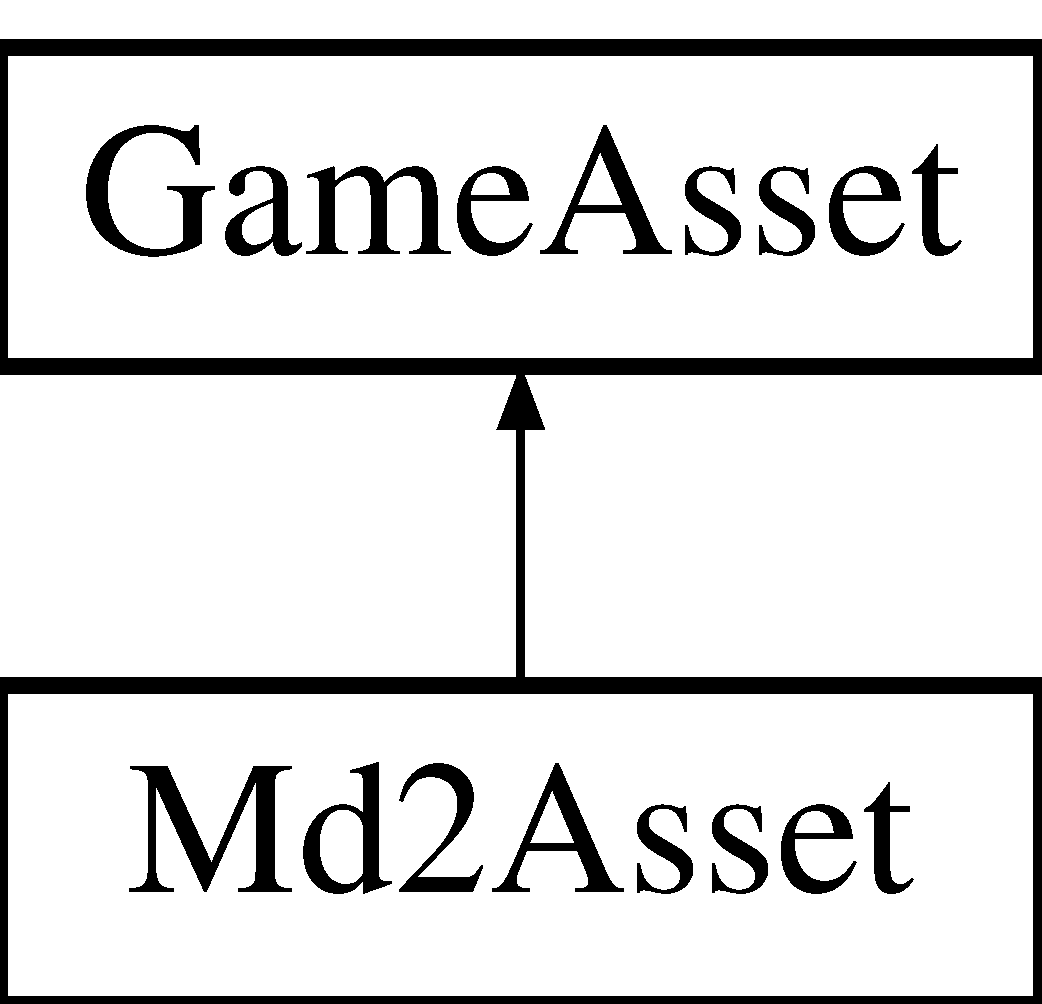
\includegraphics[height=2.000000cm]{classMd2Asset}
\end{center}
\end{figure}
\subsection*{Public Member Functions}
\begin{DoxyCompactItemize}
\item 
\hypertarget{classMd2Asset_af11c2df6a76c46c7fbcaf128ef2e5ca0}{{\bfseries Md2\-Asset} (const string \&filename)}\label{classMd2Asset_af11c2df6a76c46c7fbcaf128ef2e5ca0}

\item 
\hypertarget{classMd2Asset_a1243a6d23a9a47e5a03b8208ea9a84f5}{virtual void {\bfseries update} ()}\label{classMd2Asset_a1243a6d23a9a47e5a03b8208ea9a84f5}

\end{DoxyCompactItemize}
\subsection*{Additional Inherited Members}


\subsection{Detailed Description}


Definition at line 24 of file Md2\-Asset.\-h.



The documentation for this class was generated from the following files\-:\begin{DoxyCompactItemize}
\item 
src/Md2\-Asset.\-h\item 
src/Md2\-Asset.\-cpp\end{DoxyCompactItemize}

\hypertarget{classModelTriangle}{\section{Model\-Triangle Class Reference}
\label{classModelTriangle}\index{Model\-Triangle@{Model\-Triangle}}
}


\hyperlink{classModelTriangle}{Model\-Triangle} class.  




{\ttfamily \#include $<$Model\-Triangle.\-h$>$}

\subsection*{Public Member Functions}
\begin{DoxyCompactItemize}
\item 
\hypertarget{classModelTriangle_a3b2ac79093da14584d79f3049ad8a0f4}{{\bfseries Model\-Triangle} (\hyperlink{classVectormath_1_1Aos_1_1Point3}{Point3} p1, \hyperlink{classVectormath_1_1Aos_1_1Point3}{Point3} p2, \hyperlink{classVectormath_1_1Aos_1_1Point3}{Point3} p3)}\label{classModelTriangle_a3b2ac79093da14584d79f3049ad8a0f4}

\item 
\hypertarget{classModelTriangle_acb54b4fc644479eca37b6fd31503d126}{\hyperlink{classVectormath_1_1Aos_1_1Point3}{Point3} {\bfseries get\-Poi1} ()}\label{classModelTriangle_acb54b4fc644479eca37b6fd31503d126}

\item 
\hypertarget{classModelTriangle_ae393207cd8e9232a4bf519a6031eaaea}{\hyperlink{classVectormath_1_1Aos_1_1Point3}{Point3} {\bfseries get\-Poi2} ()}\label{classModelTriangle_ae393207cd8e9232a4bf519a6031eaaea}

\item 
\hypertarget{classModelTriangle_a5a3f447e5387491a998703276e7ea11a}{\hyperlink{classVectormath_1_1Aos_1_1Point3}{Point3} {\bfseries get\-Poi3} ()}\label{classModelTriangle_a5a3f447e5387491a998703276e7ea11a}

\item 
\hypertarget{classModelTriangle_a6026feeb8053278eee9ac78a576e2161}{\hyperlink{classVectormath_1_1Aos_1_1Vector3}{Vector3} {\bfseries get\-Normal} ()}\label{classModelTriangle_a6026feeb8053278eee9ac78a576e2161}

\item 
\hypertarget{classModelTriangle_a2961e48d38e1ac1ce0efa59e802f7e01}{\hyperlink{classVectormath_1_1Aos_1_1Vector3}{Vector3} {\bfseries get\-U} ()}\label{classModelTriangle_a2961e48d38e1ac1ce0efa59e802f7e01}

\item 
\hypertarget{classModelTriangle_a38c7778fe7c30857c769ccc70c8fb85c}{\hyperlink{classVectormath_1_1Aos_1_1Vector3}{Vector3} {\bfseries get\-V} ()}\label{classModelTriangle_a38c7778fe7c30857c769ccc70c8fb85c}

\end{DoxyCompactItemize}


\subsection{Detailed Description}
\hyperlink{classModelTriangle}{Model\-Triangle} class. 

This class is a triangle made up of 3 3\-D points. Used for Polygon soup collision detection and model loading. Not currently used. 

Definition at line 26 of file Model\-Triangle.\-h.



The documentation for this class was generated from the following files\-:\begin{DoxyCompactItemize}
\item 
src/Model\-Triangle.\-h\item 
src/Model\-Triangle.\-cpp\end{DoxyCompactItemize}

\hypertarget{classPhysics}{\section{Physics Class Reference}
\label{classPhysics}\index{Physics@{Physics}}
}


\hyperlink{classPhysics}{Physics} Class.  




{\ttfamily \#include $<$Physics.\-h$>$}

\subsection*{Public Member Functions}
\begin{DoxyCompactItemize}
\item 
\hypertarget{classPhysics_a4b8707330563fb1f9c7928e401f148fc}{{\bfseries Physics} (\hyperlink{classData}{Data} $\ast$d)}\label{classPhysics_a4b8707330563fb1f9c7928e401f148fc}

\item 
\hypertarget{classPhysics_a06548de8c46a0f5221a0489f99089ff4}{void \hyperlink{classPhysics_a06548de8c46a0f5221a0489f99089ff4}{start\-Game} ()}\label{classPhysics_a06548de8c46a0f5221a0489f99089ff4}

\begin{DoxyCompactList}\small\item\em Start Method. \end{DoxyCompactList}\item 
\hypertarget{classPhysics_a7fcfb97c9556a6ecb6d2753a7f54a5ed}{void \hyperlink{classPhysics_a7fcfb97c9556a6ecb6d2753a7f54a5ed}{update\-Data} ()}\label{classPhysics_a7fcfb97c9556a6ecb6d2753a7f54a5ed}

\begin{DoxyCompactList}\small\item\em Update Method. \end{DoxyCompactList}\item 
\hypertarget{classPhysics_a0de42b58ef325184c2d7680682e5e7f9}{bool \hyperlink{classPhysics_a0de42b58ef325184c2d7680682e5e7f9}{get\-Col} (shared\-\_\-ptr$<$ \hyperlink{classGameAsset}{Game\-Asset} $>$ ob1, shared\-\_\-ptr$<$ \hyperlink{classGameAsset}{Game\-Asset} $>$ ob2)}\label{classPhysics_a0de42b58ef325184c2d7680682e5e7f9}

\begin{DoxyCompactList}\small\item\em Collision Method. \end{DoxyCompactList}\item 
\hypertarget{classPhysics_ab91b6ab5e220174562c0186f335749d2}{bool \hyperlink{classPhysics_ab91b6ab5e220174562c0186f335749d2}{sea\-Vec} (vector$<$ Global\-::\-Force $>$ v, Global\-::\-Force f)}\label{classPhysics_ab91b6ab5e220174562c0186f335749d2}

\begin{DoxyCompactList}\small\item\em Search Vector. \end{DoxyCompactList}\item 
\hypertarget{classPhysics_a18d6624118907a527a1ac69878a39f95}{bool \hyperlink{classPhysics_a18d6624118907a527a1ac69878a39f95}{mov\-Col} (shared\-\_\-ptr$<$ \hyperlink{classGameAsset}{Game\-Asset} $>$ ob1, char d, float m)}\label{classPhysics_a18d6624118907a527a1ac69878a39f95}

\begin{DoxyCompactList}\small\item\em Movement collision. \end{DoxyCompactList}\end{DoxyCompactItemize}


\subsection{Detailed Description}
\hyperlink{classPhysics}{Physics} Class. 

A simple class that handles the updates of objects including collision. 

Definition at line 29 of file Physics.\-h.



The documentation for this class was generated from the following files\-:\begin{DoxyCompactItemize}
\item 
src/Physics.\-h\item 
src/Physics.\-cpp\end{DoxyCompactItemize}

\hypertarget{classVectormath_1_1Soa_1_1Point3}{\section{Vectormath\-:\-:Soa\-:\-:Point3 Class Reference}
\label{classVectormath_1_1Soa_1_1Point3}\index{Vectormath\-::\-Soa\-::\-Point3@{Vectormath\-::\-Soa\-::\-Point3}}
}
\subsection*{Public Member Functions}
\begin{DoxyCompactItemize}
\item 
\hypertarget{classVectormath_1_1Soa_1_1Point3_aab495c0f0e3246b4505fb1539ba43fba}{{\bfseries Point3} (const \hyperlink{classVectormath_1_1Soa_1_1Point3}{Point3} \&pnt)}\label{classVectormath_1_1Soa_1_1Point3_aab495c0f0e3246b4505fb1539ba43fba}

\item 
\hypertarget{classVectormath_1_1Soa_1_1Point3_afa048556fb5733155f7570b98041c6aa}{{\bfseries Point3} (vec\-\_\-float4 x, vec\-\_\-float4 y, vec\-\_\-float4 z)}\label{classVectormath_1_1Soa_1_1Point3_afa048556fb5733155f7570b98041c6aa}

\item 
\hypertarget{classVectormath_1_1Soa_1_1Point3_a069cd5b9fcba74fd59d31745b43fd6cd}{{\bfseries Point3} (const \hyperlink{classVectormath_1_1Soa_1_1Vector3}{Vector3} \&vec)}\label{classVectormath_1_1Soa_1_1Point3_a069cd5b9fcba74fd59d31745b43fd6cd}

\item 
\hypertarget{classVectormath_1_1Soa_1_1Point3_a218e3dfa22fd1586999dc4a9a6839607}{{\bfseries Point3} (vec\-\_\-float4 scalar)}\label{classVectormath_1_1Soa_1_1Point3_a218e3dfa22fd1586999dc4a9a6839607}

\item 
\hypertarget{classVectormath_1_1Soa_1_1Point3_a7e914a6b7473102541aaa17017b62050}{{\bfseries Point3} (\hyperlink{classVectormath_1_1Aos_1_1Point3}{Aos\-::\-Point3} pnt)}\label{classVectormath_1_1Soa_1_1Point3_a7e914a6b7473102541aaa17017b62050}

\item 
\hypertarget{classVectormath_1_1Soa_1_1Point3_a59166c3fd55027427b8c2e130a71e907}{{\bfseries Point3} (\hyperlink{classVectormath_1_1Aos_1_1Point3}{Aos\-::\-Point3} pnt0, \hyperlink{classVectormath_1_1Aos_1_1Point3}{Aos\-::\-Point3} pnt1, \hyperlink{classVectormath_1_1Aos_1_1Point3}{Aos\-::\-Point3} pnt2, \hyperlink{classVectormath_1_1Aos_1_1Point3}{Aos\-::\-Point3} pnt3)}\label{classVectormath_1_1Soa_1_1Point3_a59166c3fd55027427b8c2e130a71e907}

\item 
\hypertarget{classVectormath_1_1Soa_1_1Point3_a1f95d915761ce2c5b9e5c96d5b2c88f2}{void {\bfseries get4\-Aos} (\hyperlink{classVectormath_1_1Aos_1_1Point3}{Aos\-::\-Point3} \&result0, \hyperlink{classVectormath_1_1Aos_1_1Point3}{Aos\-::\-Point3} \&result1, \hyperlink{classVectormath_1_1Aos_1_1Point3}{Aos\-::\-Point3} \&result2, \hyperlink{classVectormath_1_1Aos_1_1Point3}{Aos\-::\-Point3} \&result3) const }\label{classVectormath_1_1Soa_1_1Point3_a1f95d915761ce2c5b9e5c96d5b2c88f2}

\item 
\hypertarget{classVectormath_1_1Soa_1_1Point3_a0cdcb6e44e39a5b754e8357ba9425c24}{\hyperlink{classVectormath_1_1Soa_1_1Point3}{Point3} \& {\bfseries operator=} (const \hyperlink{classVectormath_1_1Soa_1_1Point3}{Point3} \&pnt)}\label{classVectormath_1_1Soa_1_1Point3_a0cdcb6e44e39a5b754e8357ba9425c24}

\item 
\hypertarget{classVectormath_1_1Soa_1_1Point3_ab1eb65432aac8cfccf5dcd7ed19cefc7}{\hyperlink{classVectormath_1_1Soa_1_1Point3}{Point3} \& {\bfseries set\-X} (vec\-\_\-float4 x)}\label{classVectormath_1_1Soa_1_1Point3_ab1eb65432aac8cfccf5dcd7ed19cefc7}

\item 
\hypertarget{classVectormath_1_1Soa_1_1Point3_a75d120042c728a367c84d3bdd00481d5}{\hyperlink{classVectormath_1_1Soa_1_1Point3}{Point3} \& {\bfseries set\-Y} (vec\-\_\-float4 y)}\label{classVectormath_1_1Soa_1_1Point3_a75d120042c728a367c84d3bdd00481d5}

\item 
\hypertarget{classVectormath_1_1Soa_1_1Point3_ad1478b32aeaa62ee1ad088edfd03941a}{\hyperlink{classVectormath_1_1Soa_1_1Point3}{Point3} \& {\bfseries set\-Z} (vec\-\_\-float4 z)}\label{classVectormath_1_1Soa_1_1Point3_ad1478b32aeaa62ee1ad088edfd03941a}

\item 
\hypertarget{classVectormath_1_1Soa_1_1Point3_acd60f9abe615c0f5aa0af82342cc6c15}{vec\-\_\-float4 {\bfseries get\-X} () const }\label{classVectormath_1_1Soa_1_1Point3_acd60f9abe615c0f5aa0af82342cc6c15}

\item 
\hypertarget{classVectormath_1_1Soa_1_1Point3_ab929c1c266f9f621070a1dfaaed8b769}{vec\-\_\-float4 {\bfseries get\-Y} () const }\label{classVectormath_1_1Soa_1_1Point3_ab929c1c266f9f621070a1dfaaed8b769}

\item 
\hypertarget{classVectormath_1_1Soa_1_1Point3_a943e670c29dae716d8d085b3b94bd374}{vec\-\_\-float4 {\bfseries get\-Z} () const }\label{classVectormath_1_1Soa_1_1Point3_a943e670c29dae716d8d085b3b94bd374}

\item 
\hypertarget{classVectormath_1_1Soa_1_1Point3_a32724f0ba04bcb07f8b05d78f4a9bf02}{\hyperlink{classVectormath_1_1Soa_1_1Point3}{Point3} \& {\bfseries set\-Elem} (int idx, vec\-\_\-float4 value)}\label{classVectormath_1_1Soa_1_1Point3_a32724f0ba04bcb07f8b05d78f4a9bf02}

\item 
\hypertarget{classVectormath_1_1Soa_1_1Point3_ac83e9baae7843966a73c44aa8ea8f191}{vec\-\_\-float4 {\bfseries get\-Elem} (int idx) const }\label{classVectormath_1_1Soa_1_1Point3_ac83e9baae7843966a73c44aa8ea8f191}

\item 
\hypertarget{classVectormath_1_1Soa_1_1Point3_a2786b83175682215a62d9776a840eec9}{vec\-\_\-float4\-\_\-t \& {\bfseries operator\mbox{[}$\,$\mbox{]}} (int idx)}\label{classVectormath_1_1Soa_1_1Point3_a2786b83175682215a62d9776a840eec9}

\item 
\hypertarget{classVectormath_1_1Soa_1_1Point3_a85d222b26f998d22adeba4b1a9c8506f}{vec\-\_\-float4 {\bfseries operator\mbox{[}$\,$\mbox{]}} (int idx) const }\label{classVectormath_1_1Soa_1_1Point3_a85d222b26f998d22adeba4b1a9c8506f}

\item 
\hypertarget{classVectormath_1_1Soa_1_1Point3_a82c1d800bd31dd5d3926d365d2c1acd0}{const \hyperlink{classVectormath_1_1Soa_1_1Vector3}{Vector3} {\bfseries operator-\/} (const \hyperlink{classVectormath_1_1Soa_1_1Point3}{Point3} \&pnt) const }\label{classVectormath_1_1Soa_1_1Point3_a82c1d800bd31dd5d3926d365d2c1acd0}

\item 
\hypertarget{classVectormath_1_1Soa_1_1Point3_ac77bb6fc67c50a0fe2ce7df62b08f5c4}{const \hyperlink{classVectormath_1_1Soa_1_1Point3}{Point3} {\bfseries operator+} (const \hyperlink{classVectormath_1_1Soa_1_1Vector3}{Vector3} \&vec) const }\label{classVectormath_1_1Soa_1_1Point3_ac77bb6fc67c50a0fe2ce7df62b08f5c4}

\item 
\hypertarget{classVectormath_1_1Soa_1_1Point3_abd8b13c7d8f776635be3de6dbe984e9f}{const \hyperlink{classVectormath_1_1Soa_1_1Point3}{Point3} {\bfseries operator-\/} (const \hyperlink{classVectormath_1_1Soa_1_1Vector3}{Vector3} \&vec) const }\label{classVectormath_1_1Soa_1_1Point3_abd8b13c7d8f776635be3de6dbe984e9f}

\item 
\hypertarget{classVectormath_1_1Soa_1_1Point3_ac04915ed7fdc2e6957675379c1865030}{\hyperlink{classVectormath_1_1Soa_1_1Point3}{Point3} \& {\bfseries operator+=} (const \hyperlink{classVectormath_1_1Soa_1_1Vector3}{Vector3} \&vec)}\label{classVectormath_1_1Soa_1_1Point3_ac04915ed7fdc2e6957675379c1865030}

\item 
\hypertarget{classVectormath_1_1Soa_1_1Point3_a98f7ae66ceec53f53c1e9fe6d52350d8}{\hyperlink{classVectormath_1_1Soa_1_1Point3}{Point3} \& {\bfseries operator-\/=} (const \hyperlink{classVectormath_1_1Soa_1_1Vector3}{Vector3} \&vec)}\label{classVectormath_1_1Soa_1_1Point3_a98f7ae66ceec53f53c1e9fe6d52350d8}

\item 
\hypertarget{classVectormath_1_1Soa_1_1Point3_aab495c0f0e3246b4505fb1539ba43fba}{{\bfseries Point3} (const \hyperlink{classVectormath_1_1Soa_1_1Point3}{Point3} \&pnt)}\label{classVectormath_1_1Soa_1_1Point3_aab495c0f0e3246b4505fb1539ba43fba}

\item 
\hypertarget{classVectormath_1_1Soa_1_1Point3_afa048556fb5733155f7570b98041c6aa}{{\bfseries Point3} (vec\-\_\-float4 x, vec\-\_\-float4 y, vec\-\_\-float4 z)}\label{classVectormath_1_1Soa_1_1Point3_afa048556fb5733155f7570b98041c6aa}

\item 
\hypertarget{classVectormath_1_1Soa_1_1Point3_a069cd5b9fcba74fd59d31745b43fd6cd}{{\bfseries Point3} (const \hyperlink{classVectormath_1_1Soa_1_1Vector3}{Vector3} \&vec)}\label{classVectormath_1_1Soa_1_1Point3_a069cd5b9fcba74fd59d31745b43fd6cd}

\item 
\hypertarget{classVectormath_1_1Soa_1_1Point3_a218e3dfa22fd1586999dc4a9a6839607}{{\bfseries Point3} (vec\-\_\-float4 scalar)}\label{classVectormath_1_1Soa_1_1Point3_a218e3dfa22fd1586999dc4a9a6839607}

\item 
\hypertarget{classVectormath_1_1Soa_1_1Point3_a7e914a6b7473102541aaa17017b62050}{{\bfseries Point3} (\hyperlink{classVectormath_1_1Aos_1_1Point3}{Aos\-::\-Point3} pnt)}\label{classVectormath_1_1Soa_1_1Point3_a7e914a6b7473102541aaa17017b62050}

\item 
\hypertarget{classVectormath_1_1Soa_1_1Point3_a59166c3fd55027427b8c2e130a71e907}{{\bfseries Point3} (\hyperlink{classVectormath_1_1Aos_1_1Point3}{Aos\-::\-Point3} pnt0, \hyperlink{classVectormath_1_1Aos_1_1Point3}{Aos\-::\-Point3} pnt1, \hyperlink{classVectormath_1_1Aos_1_1Point3}{Aos\-::\-Point3} pnt2, \hyperlink{classVectormath_1_1Aos_1_1Point3}{Aos\-::\-Point3} pnt3)}\label{classVectormath_1_1Soa_1_1Point3_a59166c3fd55027427b8c2e130a71e907}

\item 
\hypertarget{classVectormath_1_1Soa_1_1Point3_a1f95d915761ce2c5b9e5c96d5b2c88f2}{void {\bfseries get4\-Aos} (\hyperlink{classVectormath_1_1Aos_1_1Point3}{Aos\-::\-Point3} \&result0, \hyperlink{classVectormath_1_1Aos_1_1Point3}{Aos\-::\-Point3} \&result1, \hyperlink{classVectormath_1_1Aos_1_1Point3}{Aos\-::\-Point3} \&result2, \hyperlink{classVectormath_1_1Aos_1_1Point3}{Aos\-::\-Point3} \&result3) const }\label{classVectormath_1_1Soa_1_1Point3_a1f95d915761ce2c5b9e5c96d5b2c88f2}

\item 
\hypertarget{classVectormath_1_1Soa_1_1Point3_aa6062f7c2a6d98a89199af096c471bd2}{\hyperlink{classVectormath_1_1Soa_1_1Point3}{Point3} \& {\bfseries operator=} (const \hyperlink{classVectormath_1_1Soa_1_1Point3}{Point3} \&pnt)}\label{classVectormath_1_1Soa_1_1Point3_aa6062f7c2a6d98a89199af096c471bd2}

\item 
\hypertarget{classVectormath_1_1Soa_1_1Point3_ab91287fdf6af8f9c1c824c6d5ee2c1dd}{\hyperlink{classVectormath_1_1Soa_1_1Point3}{Point3} \& {\bfseries set\-X} (vec\-\_\-float4 x)}\label{classVectormath_1_1Soa_1_1Point3_ab91287fdf6af8f9c1c824c6d5ee2c1dd}

\item 
\hypertarget{classVectormath_1_1Soa_1_1Point3_ab545d272fc3a151e2f079159c3ea3f0e}{\hyperlink{classVectormath_1_1Soa_1_1Point3}{Point3} \& {\bfseries set\-Y} (vec\-\_\-float4 y)}\label{classVectormath_1_1Soa_1_1Point3_ab545d272fc3a151e2f079159c3ea3f0e}

\item 
\hypertarget{classVectormath_1_1Soa_1_1Point3_a9bf755a65b93a8d7c8a8480288550349}{\hyperlink{classVectormath_1_1Soa_1_1Point3}{Point3} \& {\bfseries set\-Z} (vec\-\_\-float4 z)}\label{classVectormath_1_1Soa_1_1Point3_a9bf755a65b93a8d7c8a8480288550349}

\item 
\hypertarget{classVectormath_1_1Soa_1_1Point3_acd60f9abe615c0f5aa0af82342cc6c15}{vec\-\_\-float4 {\bfseries get\-X} () const }\label{classVectormath_1_1Soa_1_1Point3_acd60f9abe615c0f5aa0af82342cc6c15}

\item 
\hypertarget{classVectormath_1_1Soa_1_1Point3_ab929c1c266f9f621070a1dfaaed8b769}{vec\-\_\-float4 {\bfseries get\-Y} () const }\label{classVectormath_1_1Soa_1_1Point3_ab929c1c266f9f621070a1dfaaed8b769}

\item 
\hypertarget{classVectormath_1_1Soa_1_1Point3_a943e670c29dae716d8d085b3b94bd374}{vec\-\_\-float4 {\bfseries get\-Z} () const }\label{classVectormath_1_1Soa_1_1Point3_a943e670c29dae716d8d085b3b94bd374}

\item 
\hypertarget{classVectormath_1_1Soa_1_1Point3_ab84d88a1a02dba12ab5541c985371769}{\hyperlink{classVectormath_1_1Soa_1_1Point3}{Point3} \& {\bfseries set\-Elem} (int idx, vec\-\_\-float4 value)}\label{classVectormath_1_1Soa_1_1Point3_ab84d88a1a02dba12ab5541c985371769}

\item 
\hypertarget{classVectormath_1_1Soa_1_1Point3_ac83e9baae7843966a73c44aa8ea8f191}{vec\-\_\-float4 {\bfseries get\-Elem} (int idx) const }\label{classVectormath_1_1Soa_1_1Point3_ac83e9baae7843966a73c44aa8ea8f191}

\item 
\hypertarget{classVectormath_1_1Soa_1_1Point3_a8358e39b24ff055400d2949036312a49}{vec\-\_\-float4\-\_\-t \& {\bfseries operator\mbox{[}$\,$\mbox{]}} (int idx)}\label{classVectormath_1_1Soa_1_1Point3_a8358e39b24ff055400d2949036312a49}

\item 
\hypertarget{classVectormath_1_1Soa_1_1Point3_a85d222b26f998d22adeba4b1a9c8506f}{vec\-\_\-float4 {\bfseries operator\mbox{[}$\,$\mbox{]}} (int idx) const }\label{classVectormath_1_1Soa_1_1Point3_a85d222b26f998d22adeba4b1a9c8506f}

\item 
\hypertarget{classVectormath_1_1Soa_1_1Point3_a82c1d800bd31dd5d3926d365d2c1acd0}{const \hyperlink{classVectormath_1_1Soa_1_1Vector3}{Vector3} {\bfseries operator-\/} (const \hyperlink{classVectormath_1_1Soa_1_1Point3}{Point3} \&pnt) const }\label{classVectormath_1_1Soa_1_1Point3_a82c1d800bd31dd5d3926d365d2c1acd0}

\item 
\hypertarget{classVectormath_1_1Soa_1_1Point3_ac77bb6fc67c50a0fe2ce7df62b08f5c4}{const \hyperlink{classVectormath_1_1Soa_1_1Point3}{Point3} {\bfseries operator+} (const \hyperlink{classVectormath_1_1Soa_1_1Vector3}{Vector3} \&vec) const }\label{classVectormath_1_1Soa_1_1Point3_ac77bb6fc67c50a0fe2ce7df62b08f5c4}

\item 
\hypertarget{classVectormath_1_1Soa_1_1Point3_abd8b13c7d8f776635be3de6dbe984e9f}{const \hyperlink{classVectormath_1_1Soa_1_1Point3}{Point3} {\bfseries operator-\/} (const \hyperlink{classVectormath_1_1Soa_1_1Vector3}{Vector3} \&vec) const }\label{classVectormath_1_1Soa_1_1Point3_abd8b13c7d8f776635be3de6dbe984e9f}

\item 
\hypertarget{classVectormath_1_1Soa_1_1Point3_a71f0b6d3d306c6aae2c38b4d7c565f5c}{\hyperlink{classVectormath_1_1Soa_1_1Point3}{Point3} \& {\bfseries operator+=} (const \hyperlink{classVectormath_1_1Soa_1_1Vector3}{Vector3} \&vec)}\label{classVectormath_1_1Soa_1_1Point3_a71f0b6d3d306c6aae2c38b4d7c565f5c}

\item 
\hypertarget{classVectormath_1_1Soa_1_1Point3_a8101822f9ee098b0f923d33b66a52f9f}{\hyperlink{classVectormath_1_1Soa_1_1Point3}{Point3} \& {\bfseries operator-\/=} (const \hyperlink{classVectormath_1_1Soa_1_1Vector3}{Vector3} \&vec)}\label{classVectormath_1_1Soa_1_1Point3_a8101822f9ee098b0f923d33b66a52f9f}

\end{DoxyCompactItemize}


\subsection{Detailed Description}


Definition at line 638 of file vectormath\-\_\-soa.\-h.



The documentation for this class was generated from the following files\-:\begin{DoxyCompactItemize}
\item 
src/include/vectormath/ppu/cpp/vectormath\-\_\-soa.\-h\item 
src/include/vectormath/ppu/cpp/vec\-\_\-soa.\-h\end{DoxyCompactItemize}

\hypertarget{classVectormath_1_1Aos_1_1Point3}{\section{Vectormath\-:\-:Aos\-:\-:Point3 Class Reference}
\label{classVectormath_1_1Aos_1_1Point3}\index{Vectormath\-::\-Aos\-::\-Point3@{Vectormath\-::\-Aos\-::\-Point3}}
}
\subsection*{Public Member Functions}
\begin{DoxyCompactItemize}
\item 
\hypertarget{classVectormath_1_1Aos_1_1Point3_afefef06db5576da6ba658e4a5d3447b4}{{\bfseries Point3} (float x, float y, float z)}\label{classVectormath_1_1Aos_1_1Point3_afefef06db5576da6ba658e4a5d3447b4}

\item 
\hypertarget{classVectormath_1_1Aos_1_1Point3_af353dd389e12cd4510d06b62689431c4}{{\bfseries Point3} (\hyperlink{classVectormath_1_1floatInVec}{float\-In\-Vec} x, \hyperlink{classVectormath_1_1floatInVec}{float\-In\-Vec} y, \hyperlink{classVectormath_1_1floatInVec}{float\-In\-Vec} z)}\label{classVectormath_1_1Aos_1_1Point3_af353dd389e12cd4510d06b62689431c4}

\item 
\hypertarget{classVectormath_1_1Aos_1_1Point3_a89ff2e36b3e1768a9c2ea50fbe72786f}{{\bfseries Point3} (\hyperlink{classVectormath_1_1Aos_1_1Vector3}{Vector3} vec)}\label{classVectormath_1_1Aos_1_1Point3_a89ff2e36b3e1768a9c2ea50fbe72786f}

\item 
\hypertarget{classVectormath_1_1Aos_1_1Point3_ad462a241848fca89c3954860302a7167}{{\bfseries Point3} (float scalar)}\label{classVectormath_1_1Aos_1_1Point3_ad462a241848fca89c3954860302a7167}

\item 
\hypertarget{classVectormath_1_1Aos_1_1Point3_a92d23f9ab46d8741d4420ba6a4a4c05f}{{\bfseries Point3} (\hyperlink{classVectormath_1_1floatInVec}{float\-In\-Vec} scalar)}\label{classVectormath_1_1Aos_1_1Point3_a92d23f9ab46d8741d4420ba6a4a4c05f}

\item 
\hypertarget{classVectormath_1_1Aos_1_1Point3_afa6a16552c58506d969521a32a16d46b}{{\bfseries Point3} (vec\-\_\-float4 vf4)}\label{classVectormath_1_1Aos_1_1Point3_afa6a16552c58506d969521a32a16d46b}

\item 
\hypertarget{classVectormath_1_1Aos_1_1Point3_a35a02b9e0dd8f87de7edbd1f9692128d}{vec\-\_\-float4 {\bfseries get128} () const }\label{classVectormath_1_1Aos_1_1Point3_a35a02b9e0dd8f87de7edbd1f9692128d}

\item 
\hypertarget{classVectormath_1_1Aos_1_1Point3_a3ae30c30895389a2055d00f96bc9d0c7}{\hyperlink{classVectormath_1_1Aos_1_1Point3}{Point3} \& {\bfseries operator=} (\hyperlink{classVectormath_1_1Aos_1_1Point3}{Point3} pnt)}\label{classVectormath_1_1Aos_1_1Point3_a3ae30c30895389a2055d00f96bc9d0c7}

\item 
\hypertarget{classVectormath_1_1Aos_1_1Point3_aafa662e8861578a756722ac2c40b510d}{\hyperlink{classVectormath_1_1Aos_1_1Point3}{Point3} \& {\bfseries set\-X} (float x)}\label{classVectormath_1_1Aos_1_1Point3_aafa662e8861578a756722ac2c40b510d}

\item 
\hypertarget{classVectormath_1_1Aos_1_1Point3_a5a9d3e42bf62c89f698263e7aa764e1b}{\hyperlink{classVectormath_1_1Aos_1_1Point3}{Point3} \& {\bfseries set\-Y} (float y)}\label{classVectormath_1_1Aos_1_1Point3_a5a9d3e42bf62c89f698263e7aa764e1b}

\item 
\hypertarget{classVectormath_1_1Aos_1_1Point3_a3605288c7f14eb03573dca7c4d1dc51d}{\hyperlink{classVectormath_1_1Aos_1_1Point3}{Point3} \& {\bfseries set\-Z} (float z)}\label{classVectormath_1_1Aos_1_1Point3_a3605288c7f14eb03573dca7c4d1dc51d}

\item 
\hypertarget{classVectormath_1_1Aos_1_1Point3_a82820021afe676f6305d0981521a184b}{\hyperlink{classVectormath_1_1Aos_1_1Point3}{Point3} \& {\bfseries set\-X} (\hyperlink{classVectormath_1_1floatInVec}{float\-In\-Vec} x)}\label{classVectormath_1_1Aos_1_1Point3_a82820021afe676f6305d0981521a184b}

\item 
\hypertarget{classVectormath_1_1Aos_1_1Point3_a1ed105494bc1be8b1f2d72ffd953446b}{\hyperlink{classVectormath_1_1Aos_1_1Point3}{Point3} \& {\bfseries set\-Y} (\hyperlink{classVectormath_1_1floatInVec}{float\-In\-Vec} y)}\label{classVectormath_1_1Aos_1_1Point3_a1ed105494bc1be8b1f2d72ffd953446b}

\item 
\hypertarget{classVectormath_1_1Aos_1_1Point3_a64159cb82443953f3c020c1ab194d9d5}{\hyperlink{classVectormath_1_1Aos_1_1Point3}{Point3} \& {\bfseries set\-Z} (\hyperlink{classVectormath_1_1floatInVec}{float\-In\-Vec} z)}\label{classVectormath_1_1Aos_1_1Point3_a64159cb82443953f3c020c1ab194d9d5}

\item 
\hypertarget{classVectormath_1_1Aos_1_1Point3_addf7a1451cf6e1e3f77648fa29d49f85}{const \hyperlink{classVectormath_1_1floatInVec}{float\-In\-Vec} {\bfseries get\-X} () const }\label{classVectormath_1_1Aos_1_1Point3_addf7a1451cf6e1e3f77648fa29d49f85}

\item 
\hypertarget{classVectormath_1_1Aos_1_1Point3_aff2b8f86f0382cc1e8f186587c7b6012}{const \hyperlink{classVectormath_1_1floatInVec}{float\-In\-Vec} {\bfseries get\-Y} () const }\label{classVectormath_1_1Aos_1_1Point3_aff2b8f86f0382cc1e8f186587c7b6012}

\item 
\hypertarget{classVectormath_1_1Aos_1_1Point3_a88bbe96362edf97c07c7877e5baf0829}{const \hyperlink{classVectormath_1_1floatInVec}{float\-In\-Vec} {\bfseries get\-Z} () const }\label{classVectormath_1_1Aos_1_1Point3_a88bbe96362edf97c07c7877e5baf0829}

\item 
\hypertarget{classVectormath_1_1Aos_1_1Point3_af552226e77f23dfee94e7010be9c19f5}{\hyperlink{classVectormath_1_1Aos_1_1Point3}{Point3} \& {\bfseries set\-Elem} (int idx, float value)}\label{classVectormath_1_1Aos_1_1Point3_af552226e77f23dfee94e7010be9c19f5}

\item 
\hypertarget{classVectormath_1_1Aos_1_1Point3_a5b543145cbb63fd063a306a00cbc0c32}{\hyperlink{classVectormath_1_1Aos_1_1Point3}{Point3} \& {\bfseries set\-Elem} (int idx, \hyperlink{classVectormath_1_1floatInVec}{float\-In\-Vec} value)}\label{classVectormath_1_1Aos_1_1Point3_a5b543145cbb63fd063a306a00cbc0c32}

\item 
\hypertarget{classVectormath_1_1Aos_1_1Point3_a4fa9d2a957b0c5cb959d0d7a33c43652}{const \hyperlink{classVectormath_1_1floatInVec}{float\-In\-Vec} {\bfseries get\-Elem} (int idx) const }\label{classVectormath_1_1Aos_1_1Point3_a4fa9d2a957b0c5cb959d0d7a33c43652}

\item 
\hypertarget{classVectormath_1_1Aos_1_1Point3_aa54dfdc82ecd8c2cd2604ed6d913291a}{\hyperlink{classVectormath_1_1Aos_1_1VecIdx}{Vec\-Idx} {\bfseries operator\mbox{[}$\,$\mbox{]}} (int idx)}\label{classVectormath_1_1Aos_1_1Point3_aa54dfdc82ecd8c2cd2604ed6d913291a}

\item 
\hypertarget{classVectormath_1_1Aos_1_1Point3_a270eb5d1eb5120ad20b5ce557cd1e3bf}{const \hyperlink{classVectormath_1_1floatInVec}{float\-In\-Vec} {\bfseries operator\mbox{[}$\,$\mbox{]}} (int idx) const }\label{classVectormath_1_1Aos_1_1Point3_a270eb5d1eb5120ad20b5ce557cd1e3bf}

\item 
\hypertarget{classVectormath_1_1Aos_1_1Point3_a2c24e50b7e53a42a6cba1c2158457005}{const \hyperlink{classVectormath_1_1Aos_1_1Vector3}{Vector3} {\bfseries operator-\/} (\hyperlink{classVectormath_1_1Aos_1_1Point3}{Point3} pnt) const }\label{classVectormath_1_1Aos_1_1Point3_a2c24e50b7e53a42a6cba1c2158457005}

\item 
\hypertarget{classVectormath_1_1Aos_1_1Point3_a487897703c837047fa0bbc73f3d148b0}{const \hyperlink{classVectormath_1_1Aos_1_1Point3}{Point3} {\bfseries operator+} (\hyperlink{classVectormath_1_1Aos_1_1Vector3}{Vector3} vec) const }\label{classVectormath_1_1Aos_1_1Point3_a487897703c837047fa0bbc73f3d148b0}

\item 
\hypertarget{classVectormath_1_1Aos_1_1Point3_ac6e96a16531b15064f12e78bfa5c32c1}{const \hyperlink{classVectormath_1_1Aos_1_1Point3}{Point3} {\bfseries operator-\/} (\hyperlink{classVectormath_1_1Aos_1_1Vector3}{Vector3} vec) const }\label{classVectormath_1_1Aos_1_1Point3_ac6e96a16531b15064f12e78bfa5c32c1}

\item 
\hypertarget{classVectormath_1_1Aos_1_1Point3_a9b0e8ad9e8e8eda0f51566087f1360a2}{\hyperlink{classVectormath_1_1Aos_1_1Point3}{Point3} \& {\bfseries operator+=} (\hyperlink{classVectormath_1_1Aos_1_1Vector3}{Vector3} vec)}\label{classVectormath_1_1Aos_1_1Point3_a9b0e8ad9e8e8eda0f51566087f1360a2}

\item 
\hypertarget{classVectormath_1_1Aos_1_1Point3_ada5560877fe4bf37fe6c8fbdd65449af}{\hyperlink{classVectormath_1_1Aos_1_1Point3}{Point3} \& {\bfseries operator-\/=} (\hyperlink{classVectormath_1_1Aos_1_1Vector3}{Vector3} vec)}\label{classVectormath_1_1Aos_1_1Point3_ada5560877fe4bf37fe6c8fbdd65449af}

\item 
\hypertarget{classVectormath_1_1Aos_1_1Point3_a03dfaf1fbce8f78dc3569e57034a3fc8}{{\bfseries Point3} (const \hyperlink{classVectormath_1_1Aos_1_1Point3}{Point3} \&pnt)}\label{classVectormath_1_1Aos_1_1Point3_a03dfaf1fbce8f78dc3569e57034a3fc8}

\item 
\hypertarget{classVectormath_1_1Aos_1_1Point3_a74641a8ac1d99934fea99880a06b58db}{{\bfseries Point3} (float x, float y, float z)}\label{classVectormath_1_1Aos_1_1Point3_a74641a8ac1d99934fea99880a06b58db}

\item 
\hypertarget{classVectormath_1_1Aos_1_1Point3_a5489cee3be2045d1a57309afeecb3a3f}{{\bfseries Point3} (const \hyperlink{classVectormath_1_1Aos_1_1Vector3}{Vector3} \&vec)}\label{classVectormath_1_1Aos_1_1Point3_a5489cee3be2045d1a57309afeecb3a3f}

\item 
\hypertarget{classVectormath_1_1Aos_1_1Point3_a52800d18e22d003682c5c2bc9dd3cef4}{{\bfseries Point3} (float scalar)}\label{classVectormath_1_1Aos_1_1Point3_a52800d18e22d003682c5c2bc9dd3cef4}

\item 
\hypertarget{classVectormath_1_1Aos_1_1Point3_a038d0f5ff4bde3faa5982626b678c115}{\hyperlink{classVectormath_1_1Aos_1_1Point3}{Point3} \& {\bfseries operator=} (const \hyperlink{classVectormath_1_1Aos_1_1Point3}{Point3} \&pnt)}\label{classVectormath_1_1Aos_1_1Point3_a038d0f5ff4bde3faa5982626b678c115}

\item 
\hypertarget{classVectormath_1_1Aos_1_1Point3_ab290dd11de0a70bf457d2907bd3392c3}{\hyperlink{classVectormath_1_1Aos_1_1Point3}{Point3} \& {\bfseries set\-X} (float x)}\label{classVectormath_1_1Aos_1_1Point3_ab290dd11de0a70bf457d2907bd3392c3}

\item 
\hypertarget{classVectormath_1_1Aos_1_1Point3_a10d06c10cbe3f0866339e872dc216b00}{\hyperlink{classVectormath_1_1Aos_1_1Point3}{Point3} \& {\bfseries set\-Y} (float y)}\label{classVectormath_1_1Aos_1_1Point3_a10d06c10cbe3f0866339e872dc216b00}

\item 
\hypertarget{classVectormath_1_1Aos_1_1Point3_af4ca752583411898ea4fc2ed87d68d03}{\hyperlink{classVectormath_1_1Aos_1_1Point3}{Point3} \& {\bfseries set\-Z} (float z)}\label{classVectormath_1_1Aos_1_1Point3_af4ca752583411898ea4fc2ed87d68d03}

\item 
\hypertarget{classVectormath_1_1Aos_1_1Point3_aae02e04a14cd7d4194ca681df958e08f}{float {\bfseries get\-X} () const }\label{classVectormath_1_1Aos_1_1Point3_aae02e04a14cd7d4194ca681df958e08f}

\item 
\hypertarget{classVectormath_1_1Aos_1_1Point3_a6d06ef54d34f7552680d1e7d672ab473}{float {\bfseries get\-Y} () const }\label{classVectormath_1_1Aos_1_1Point3_a6d06ef54d34f7552680d1e7d672ab473}

\item 
\hypertarget{classVectormath_1_1Aos_1_1Point3_ad83252a573e61cff750b1e93420d469f}{float {\bfseries get\-Z} () const }\label{classVectormath_1_1Aos_1_1Point3_ad83252a573e61cff750b1e93420d469f}

\item 
\hypertarget{classVectormath_1_1Aos_1_1Point3_a903b1268fbf9b9083f429444637c5e6d}{\hyperlink{classVectormath_1_1Aos_1_1Point3}{Point3} \& {\bfseries set\-Elem} (int idx, float value)}\label{classVectormath_1_1Aos_1_1Point3_a903b1268fbf9b9083f429444637c5e6d}

\item 
\hypertarget{classVectormath_1_1Aos_1_1Point3_a799aaab8cc96e46dffc1f14475d00a11}{float {\bfseries get\-Elem} (int idx) const }\label{classVectormath_1_1Aos_1_1Point3_a799aaab8cc96e46dffc1f14475d00a11}

\item 
\hypertarget{classVectormath_1_1Aos_1_1Point3_a555b835162f7daa0d6f942cadf2a0936}{float \& {\bfseries operator\mbox{[}$\,$\mbox{]}} (int idx)}\label{classVectormath_1_1Aos_1_1Point3_a555b835162f7daa0d6f942cadf2a0936}

\item 
\hypertarget{classVectormath_1_1Aos_1_1Point3_a3efc9e792f42d04bfb88b440c2b7f33b}{float {\bfseries operator\mbox{[}$\,$\mbox{]}} (int idx) const }\label{classVectormath_1_1Aos_1_1Point3_a3efc9e792f42d04bfb88b440c2b7f33b}

\item 
\hypertarget{classVectormath_1_1Aos_1_1Point3_ae2bf138eb808c54de541e0c5c3765220}{const \hyperlink{classVectormath_1_1Aos_1_1Vector3}{Vector3} {\bfseries operator-\/} (const \hyperlink{classVectormath_1_1Aos_1_1Point3}{Point3} \&pnt) const }\label{classVectormath_1_1Aos_1_1Point3_ae2bf138eb808c54de541e0c5c3765220}

\item 
\hypertarget{classVectormath_1_1Aos_1_1Point3_a0ce7ee8da5963f3da517bdd21e9cbbc3}{const \hyperlink{classVectormath_1_1Aos_1_1Point3}{Point3} {\bfseries operator+} (const \hyperlink{classVectormath_1_1Aos_1_1Vector3}{Vector3} \&vec) const }\label{classVectormath_1_1Aos_1_1Point3_a0ce7ee8da5963f3da517bdd21e9cbbc3}

\item 
\hypertarget{classVectormath_1_1Aos_1_1Point3_ad691653c67a2be5da1d2ef3a2792b85e}{const \hyperlink{classVectormath_1_1Aos_1_1Point3}{Point3} {\bfseries operator-\/} (const \hyperlink{classVectormath_1_1Aos_1_1Vector3}{Vector3} \&vec) const }\label{classVectormath_1_1Aos_1_1Point3_ad691653c67a2be5da1d2ef3a2792b85e}

\item 
\hypertarget{classVectormath_1_1Aos_1_1Point3_a924a091f9df9a7c348eb72ed2ea3451e}{\hyperlink{classVectormath_1_1Aos_1_1Point3}{Point3} \& {\bfseries operator+=} (const \hyperlink{classVectormath_1_1Aos_1_1Vector3}{Vector3} \&vec)}\label{classVectormath_1_1Aos_1_1Point3_a924a091f9df9a7c348eb72ed2ea3451e}

\item 
\hypertarget{classVectormath_1_1Aos_1_1Point3_ad1c0d6415b9efba4030191f6a3a09ab3}{\hyperlink{classVectormath_1_1Aos_1_1Point3}{Point3} \& {\bfseries operator-\/=} (const \hyperlink{classVectormath_1_1Aos_1_1Vector3}{Vector3} \&vec)}\label{classVectormath_1_1Aos_1_1Point3_ad1c0d6415b9efba4030191f6a3a09ab3}

\item 
\hypertarget{classVectormath_1_1Aos_1_1Point3_a74641a8ac1d99934fea99880a06b58db}{{\bfseries Point3} (float x, float y, float z)}\label{classVectormath_1_1Aos_1_1Point3_a74641a8ac1d99934fea99880a06b58db}

\item 
\hypertarget{classVectormath_1_1Aos_1_1Point3_a89ff2e36b3e1768a9c2ea50fbe72786f}{{\bfseries Point3} (\hyperlink{classVectormath_1_1Aos_1_1Vector3}{Vector3} vec)}\label{classVectormath_1_1Aos_1_1Point3_a89ff2e36b3e1768a9c2ea50fbe72786f}

\item 
\hypertarget{classVectormath_1_1Aos_1_1Point3_a52800d18e22d003682c5c2bc9dd3cef4}{{\bfseries Point3} (float scalar)}\label{classVectormath_1_1Aos_1_1Point3_a52800d18e22d003682c5c2bc9dd3cef4}

\item 
\hypertarget{classVectormath_1_1Aos_1_1Point3_ab4892b1755b28dc86e26fccb4a17dfb7}{{\bfseries Point3} (vec\-\_\-float4 vf4)}\label{classVectormath_1_1Aos_1_1Point3_ab4892b1755b28dc86e26fccb4a17dfb7}

\item 
\hypertarget{classVectormath_1_1Aos_1_1Point3_ad0489201ac889f118117ea0ca847a2bf}{vec\-\_\-float4 {\bfseries get128} () const }\label{classVectormath_1_1Aos_1_1Point3_ad0489201ac889f118117ea0ca847a2bf}

\item 
\hypertarget{classVectormath_1_1Aos_1_1Point3_aac51479b1c226e9be46546fae9cd6542}{\hyperlink{classVectormath_1_1Aos_1_1Point3}{Point3} \& {\bfseries operator=} (\hyperlink{classVectormath_1_1Aos_1_1Point3}{Point3} pnt)}\label{classVectormath_1_1Aos_1_1Point3_aac51479b1c226e9be46546fae9cd6542}

\item 
\hypertarget{classVectormath_1_1Aos_1_1Point3_ab290dd11de0a70bf457d2907bd3392c3}{\hyperlink{classVectormath_1_1Aos_1_1Point3}{Point3} \& {\bfseries set\-X} (float x)}\label{classVectormath_1_1Aos_1_1Point3_ab290dd11de0a70bf457d2907bd3392c3}

\item 
\hypertarget{classVectormath_1_1Aos_1_1Point3_a10d06c10cbe3f0866339e872dc216b00}{\hyperlink{classVectormath_1_1Aos_1_1Point3}{Point3} \& {\bfseries set\-Y} (float y)}\label{classVectormath_1_1Aos_1_1Point3_a10d06c10cbe3f0866339e872dc216b00}

\item 
\hypertarget{classVectormath_1_1Aos_1_1Point3_af4ca752583411898ea4fc2ed87d68d03}{\hyperlink{classVectormath_1_1Aos_1_1Point3}{Point3} \& {\bfseries set\-Z} (float z)}\label{classVectormath_1_1Aos_1_1Point3_af4ca752583411898ea4fc2ed87d68d03}

\item 
\hypertarget{classVectormath_1_1Aos_1_1Point3_aae02e04a14cd7d4194ca681df958e08f}{float {\bfseries get\-X} () const }\label{classVectormath_1_1Aos_1_1Point3_aae02e04a14cd7d4194ca681df958e08f}

\item 
\hypertarget{classVectormath_1_1Aos_1_1Point3_a6d06ef54d34f7552680d1e7d672ab473}{float {\bfseries get\-Y} () const }\label{classVectormath_1_1Aos_1_1Point3_a6d06ef54d34f7552680d1e7d672ab473}

\item 
\hypertarget{classVectormath_1_1Aos_1_1Point3_ad83252a573e61cff750b1e93420d469f}{float {\bfseries get\-Z} () const }\label{classVectormath_1_1Aos_1_1Point3_ad83252a573e61cff750b1e93420d469f}

\item 
\hypertarget{classVectormath_1_1Aos_1_1Point3_a903b1268fbf9b9083f429444637c5e6d}{\hyperlink{classVectormath_1_1Aos_1_1Point3}{Point3} \& {\bfseries set\-Elem} (int idx, float value)}\label{classVectormath_1_1Aos_1_1Point3_a903b1268fbf9b9083f429444637c5e6d}

\item 
\hypertarget{classVectormath_1_1Aos_1_1Point3_a799aaab8cc96e46dffc1f14475d00a11}{float {\bfseries get\-Elem} (int idx) const }\label{classVectormath_1_1Aos_1_1Point3_a799aaab8cc96e46dffc1f14475d00a11}

\item 
\hypertarget{classVectormath_1_1Aos_1_1Point3_a96270debbfc1c3d8f5e685cd543b2a40}{\hyperlink{classVectormath_1_1Aos_1_1VecIdx}{Vec\-Idx} {\bfseries operator\mbox{[}$\,$\mbox{]}} (int idx)}\label{classVectormath_1_1Aos_1_1Point3_a96270debbfc1c3d8f5e685cd543b2a40}

\item 
\hypertarget{classVectormath_1_1Aos_1_1Point3_a3efc9e792f42d04bfb88b440c2b7f33b}{float {\bfseries operator\mbox{[}$\,$\mbox{]}} (int idx) const }\label{classVectormath_1_1Aos_1_1Point3_a3efc9e792f42d04bfb88b440c2b7f33b}

\item 
\hypertarget{classVectormath_1_1Aos_1_1Point3_a2c24e50b7e53a42a6cba1c2158457005}{const \hyperlink{classVectormath_1_1Aos_1_1Vector3}{Vector3} {\bfseries operator-\/} (\hyperlink{classVectormath_1_1Aos_1_1Point3}{Point3} pnt) const }\label{classVectormath_1_1Aos_1_1Point3_a2c24e50b7e53a42a6cba1c2158457005}

\item 
\hypertarget{classVectormath_1_1Aos_1_1Point3_a487897703c837047fa0bbc73f3d148b0}{const \hyperlink{classVectormath_1_1Aos_1_1Point3}{Point3} {\bfseries operator+} (\hyperlink{classVectormath_1_1Aos_1_1Vector3}{Vector3} vec) const }\label{classVectormath_1_1Aos_1_1Point3_a487897703c837047fa0bbc73f3d148b0}

\item 
\hypertarget{classVectormath_1_1Aos_1_1Point3_ac6e96a16531b15064f12e78bfa5c32c1}{const \hyperlink{classVectormath_1_1Aos_1_1Point3}{Point3} {\bfseries operator-\/} (\hyperlink{classVectormath_1_1Aos_1_1Vector3}{Vector3} vec) const }\label{classVectormath_1_1Aos_1_1Point3_ac6e96a16531b15064f12e78bfa5c32c1}

\item 
\hypertarget{classVectormath_1_1Aos_1_1Point3_aa6b961770d2cb79a7436315c4db184d0}{\hyperlink{classVectormath_1_1Aos_1_1Point3}{Point3} \& {\bfseries operator+=} (\hyperlink{classVectormath_1_1Aos_1_1Vector3}{Vector3} vec)}\label{classVectormath_1_1Aos_1_1Point3_aa6b961770d2cb79a7436315c4db184d0}

\item 
\hypertarget{classVectormath_1_1Aos_1_1Point3_a26061337361f43dcd667d7f92d0995ac}{\hyperlink{classVectormath_1_1Aos_1_1Point3}{Point3} \& {\bfseries operator-\/=} (\hyperlink{classVectormath_1_1Aos_1_1Vector3}{Vector3} vec)}\label{classVectormath_1_1Aos_1_1Point3_a26061337361f43dcd667d7f92d0995ac}

\item 
\hypertarget{classVectormath_1_1Aos_1_1Point3_afefef06db5576da6ba658e4a5d3447b4}{\-\_\-\-\_\-forceinline {\bfseries Point3} (float x, float y, float z)}\label{classVectormath_1_1Aos_1_1Point3_afefef06db5576da6ba658e4a5d3447b4}

\item 
\hypertarget{classVectormath_1_1Aos_1_1Point3_a430894e700aa969fdbe9d6c4b58b0d0b}{\-\_\-\-\_\-forceinline {\bfseries Point3} (const \hyperlink{classVectormath_1_1floatInVec}{float\-In\-Vec} \&x, const \hyperlink{classVectormath_1_1floatInVec}{float\-In\-Vec} \&y, const \hyperlink{classVectormath_1_1floatInVec}{float\-In\-Vec} \&z)}\label{classVectormath_1_1Aos_1_1Point3_a430894e700aa969fdbe9d6c4b58b0d0b}

\item 
\hypertarget{classVectormath_1_1Aos_1_1Point3_a5489cee3be2045d1a57309afeecb3a3f}{\-\_\-\-\_\-forceinline {\bfseries Point3} (const \hyperlink{classVectormath_1_1Aos_1_1Vector3}{Vector3} \&vec)}\label{classVectormath_1_1Aos_1_1Point3_a5489cee3be2045d1a57309afeecb3a3f}

\item 
\hypertarget{classVectormath_1_1Aos_1_1Point3_ad462a241848fca89c3954860302a7167}{\-\_\-\-\_\-forceinline {\bfseries Point3} (float scalar)}\label{classVectormath_1_1Aos_1_1Point3_ad462a241848fca89c3954860302a7167}

\item 
\hypertarget{classVectormath_1_1Aos_1_1Point3_ab9b8620bab885d221c528473b028b36f}{\-\_\-\-\_\-forceinline {\bfseries Point3} (const \hyperlink{classVectormath_1_1floatInVec}{float\-In\-Vec} \&scalar)}\label{classVectormath_1_1Aos_1_1Point3_ab9b8620bab885d221c528473b028b36f}

\item 
\hypertarget{classVectormath_1_1Aos_1_1Point3_a2bd6d6f70ae7dc51b0e5d8e9a5ac7d5e}{\-\_\-\-\_\-forceinline {\bfseries Point3} (\-\_\-\-\_\-m128 vf4)}\label{classVectormath_1_1Aos_1_1Point3_a2bd6d6f70ae7dc51b0e5d8e9a5ac7d5e}

\item 
\hypertarget{classVectormath_1_1Aos_1_1Point3_a35a02b9e0dd8f87de7edbd1f9692128d}{\-\_\-\-\_\-forceinline \-\_\-\-\_\-m128 {\bfseries get128} () const }\label{classVectormath_1_1Aos_1_1Point3_a35a02b9e0dd8f87de7edbd1f9692128d}

\item 
\hypertarget{classVectormath_1_1Aos_1_1Point3_a263879f30eb4851cf0b70f09b41da972}{\-\_\-\-\_\-forceinline \hyperlink{classVectormath_1_1Aos_1_1Point3}{Point3} \& {\bfseries operator=} (const \hyperlink{classVectormath_1_1Aos_1_1Point3}{Point3} \&pnt)}\label{classVectormath_1_1Aos_1_1Point3_a263879f30eb4851cf0b70f09b41da972}

\item 
\hypertarget{classVectormath_1_1Aos_1_1Point3_ab3ba5d285b84e668c2e101c609e79e3e}{\-\_\-\-\_\-forceinline \hyperlink{classVectormath_1_1Aos_1_1Point3}{Point3} \& {\bfseries set\-X} (float x)}\label{classVectormath_1_1Aos_1_1Point3_ab3ba5d285b84e668c2e101c609e79e3e}

\item 
\hypertarget{classVectormath_1_1Aos_1_1Point3_ac35c146c0408983f746e1f958ec4ed88}{\-\_\-\-\_\-forceinline \hyperlink{classVectormath_1_1Aos_1_1Point3}{Point3} \& {\bfseries set\-Y} (float y)}\label{classVectormath_1_1Aos_1_1Point3_ac35c146c0408983f746e1f958ec4ed88}

\item 
\hypertarget{classVectormath_1_1Aos_1_1Point3_ae8c8b0519aa48224713c64ae5da442a2}{\-\_\-\-\_\-forceinline \hyperlink{classVectormath_1_1Aos_1_1Point3}{Point3} \& {\bfseries set\-Z} (float z)}\label{classVectormath_1_1Aos_1_1Point3_ae8c8b0519aa48224713c64ae5da442a2}

\item 
\hypertarget{classVectormath_1_1Aos_1_1Point3_a2ceca3985ac2c77aaa7e5e35cf089c4f}{\-\_\-\-\_\-forceinline \hyperlink{classVectormath_1_1Aos_1_1Point3}{Point3} \& {\bfseries set\-X} (const \hyperlink{classVectormath_1_1floatInVec}{float\-In\-Vec} \&x)}\label{classVectormath_1_1Aos_1_1Point3_a2ceca3985ac2c77aaa7e5e35cf089c4f}

\item 
\hypertarget{classVectormath_1_1Aos_1_1Point3_acc2d6433cbe03cc03690a049aeb9bb41}{\-\_\-\-\_\-forceinline \hyperlink{classVectormath_1_1Aos_1_1Point3}{Point3} \& {\bfseries set\-Y} (const \hyperlink{classVectormath_1_1floatInVec}{float\-In\-Vec} \&y)}\label{classVectormath_1_1Aos_1_1Point3_acc2d6433cbe03cc03690a049aeb9bb41}

\item 
\hypertarget{classVectormath_1_1Aos_1_1Point3_a012adb56f51af4da5ba0cea81ab69efb}{\-\_\-\-\_\-forceinline \hyperlink{classVectormath_1_1Aos_1_1Point3}{Point3} \& {\bfseries set\-Z} (const \hyperlink{classVectormath_1_1floatInVec}{float\-In\-Vec} \&z)}\label{classVectormath_1_1Aos_1_1Point3_a012adb56f51af4da5ba0cea81ab69efb}

\item 
\hypertarget{classVectormath_1_1Aos_1_1Point3_addf7a1451cf6e1e3f77648fa29d49f85}{\-\_\-\-\_\-forceinline const \hyperlink{classVectormath_1_1floatInVec}{float\-In\-Vec} {\bfseries get\-X} () const }\label{classVectormath_1_1Aos_1_1Point3_addf7a1451cf6e1e3f77648fa29d49f85}

\item 
\hypertarget{classVectormath_1_1Aos_1_1Point3_aff2b8f86f0382cc1e8f186587c7b6012}{\-\_\-\-\_\-forceinline const \hyperlink{classVectormath_1_1floatInVec}{float\-In\-Vec} {\bfseries get\-Y} () const }\label{classVectormath_1_1Aos_1_1Point3_aff2b8f86f0382cc1e8f186587c7b6012}

\item 
\hypertarget{classVectormath_1_1Aos_1_1Point3_a88bbe96362edf97c07c7877e5baf0829}{\-\_\-\-\_\-forceinline const \hyperlink{classVectormath_1_1floatInVec}{float\-In\-Vec} {\bfseries get\-Z} () const }\label{classVectormath_1_1Aos_1_1Point3_a88bbe96362edf97c07c7877e5baf0829}

\item 
\hypertarget{classVectormath_1_1Aos_1_1Point3_aa072bc357227e67527eb53e586733b5a}{\-\_\-\-\_\-forceinline \hyperlink{classVectormath_1_1Aos_1_1Point3}{Point3} \& {\bfseries set\-Elem} (int idx, float value)}\label{classVectormath_1_1Aos_1_1Point3_aa072bc357227e67527eb53e586733b5a}

\item 
\hypertarget{classVectormath_1_1Aos_1_1Point3_a7c9413786b2e1359646ef19f34d8bf67}{\-\_\-\-\_\-forceinline \hyperlink{classVectormath_1_1Aos_1_1Point3}{Point3} \& {\bfseries set\-Elem} (int idx, const \hyperlink{classVectormath_1_1floatInVec}{float\-In\-Vec} \&value)}\label{classVectormath_1_1Aos_1_1Point3_a7c9413786b2e1359646ef19f34d8bf67}

\item 
\hypertarget{classVectormath_1_1Aos_1_1Point3_a4fa9d2a957b0c5cb959d0d7a33c43652}{\-\_\-\-\_\-forceinline const \hyperlink{classVectormath_1_1floatInVec}{float\-In\-Vec} {\bfseries get\-Elem} (int idx) const }\label{classVectormath_1_1Aos_1_1Point3_a4fa9d2a957b0c5cb959d0d7a33c43652}

\item 
\hypertarget{classVectormath_1_1Aos_1_1Point3_aa54dfdc82ecd8c2cd2604ed6d913291a}{\-\_\-\-\_\-forceinline \hyperlink{classVectormath_1_1Aos_1_1VecIdx}{Vec\-Idx} {\bfseries operator\mbox{[}$\,$\mbox{]}} (int idx)}\label{classVectormath_1_1Aos_1_1Point3_aa54dfdc82ecd8c2cd2604ed6d913291a}

\item 
\hypertarget{classVectormath_1_1Aos_1_1Point3_a270eb5d1eb5120ad20b5ce557cd1e3bf}{\-\_\-\-\_\-forceinline const \hyperlink{classVectormath_1_1floatInVec}{float\-In\-Vec} {\bfseries operator\mbox{[}$\,$\mbox{]}} (int idx) const }\label{classVectormath_1_1Aos_1_1Point3_a270eb5d1eb5120ad20b5ce557cd1e3bf}

\item 
\hypertarget{classVectormath_1_1Aos_1_1Point3_ae2bf138eb808c54de541e0c5c3765220}{\-\_\-\-\_\-forceinline const \hyperlink{classVectormath_1_1Aos_1_1Vector3}{Vector3} {\bfseries operator-\/} (const \hyperlink{classVectormath_1_1Aos_1_1Point3}{Point3} \&pnt) const }\label{classVectormath_1_1Aos_1_1Point3_ae2bf138eb808c54de541e0c5c3765220}

\item 
\hypertarget{classVectormath_1_1Aos_1_1Point3_a0ce7ee8da5963f3da517bdd21e9cbbc3}{\-\_\-\-\_\-forceinline const \hyperlink{classVectormath_1_1Aos_1_1Point3}{Point3} {\bfseries operator+} (const \hyperlink{classVectormath_1_1Aos_1_1Vector3}{Vector3} \&vec) const }\label{classVectormath_1_1Aos_1_1Point3_a0ce7ee8da5963f3da517bdd21e9cbbc3}

\item 
\hypertarget{classVectormath_1_1Aos_1_1Point3_ad691653c67a2be5da1d2ef3a2792b85e}{\-\_\-\-\_\-forceinline const \hyperlink{classVectormath_1_1Aos_1_1Point3}{Point3} {\bfseries operator-\/} (const \hyperlink{classVectormath_1_1Aos_1_1Vector3}{Vector3} \&vec) const }\label{classVectormath_1_1Aos_1_1Point3_ad691653c67a2be5da1d2ef3a2792b85e}

\item 
\hypertarget{classVectormath_1_1Aos_1_1Point3_a25c06a0a4def80955ecc05fec237e5ad}{\-\_\-\-\_\-forceinline \hyperlink{classVectormath_1_1Aos_1_1Point3}{Point3} \& {\bfseries operator+=} (const \hyperlink{classVectormath_1_1Aos_1_1Vector3}{Vector3} \&vec)}\label{classVectormath_1_1Aos_1_1Point3_a25c06a0a4def80955ecc05fec237e5ad}

\item 
\hypertarget{classVectormath_1_1Aos_1_1Point3_a370113f0a01cc6e456b54e3cd949d5d7}{\-\_\-\-\_\-forceinline \hyperlink{classVectormath_1_1Aos_1_1Point3}{Point3} \& {\bfseries operator-\/=} (const \hyperlink{classVectormath_1_1Aos_1_1Vector3}{Vector3} \&vec)}\label{classVectormath_1_1Aos_1_1Point3_a370113f0a01cc6e456b54e3cd949d5d7}

\end{DoxyCompactItemize}


The documentation for this class was generated from the following files\-:\begin{DoxyCompactItemize}
\item 
src/include/vectormath/ppu/cpp/vectormath\-\_\-aos.\-h\item 
src/include/vectormath/ppu/cpp/vec\-\_\-aos.\-h\end{DoxyCompactItemize}

\hypertarget{classPolygonTest}{\section{Polygon\-Test Class Reference}
\label{classPolygonTest}\index{Polygon\-Test@{Polygon\-Test}}
}


\hyperlink{classPolygonTest}{Polygon\-Test} Class.  




{\ttfamily \#include $<$Polygon\-Test.\-h$>$}

\subsection*{Static Public Member Functions}
\begin{DoxyCompactItemize}
\item 
static bool \hyperlink{classPolygonTest_ab56c72cf8f725173b1b61377584246ae}{get\-Collision} (vector$<$ \hyperlink{classModelTriangle}{Model\-Triangle} $>$ t\-L1, vector$<$ \hyperlink{classModelTriangle}{Model\-Triangle} $>$ t\-L2)
\end{DoxyCompactItemize}


\subsection{Detailed Description}
\hyperlink{classPolygonTest}{Polygon\-Test} Class. 

This class is designed to use Polygon soup collision detection. Currently not working. 

Definition at line 28 of file Polygon\-Test.\-h.



\subsection{Member Function Documentation}
\hypertarget{classPolygonTest_ab56c72cf8f725173b1b61377584246ae}{\index{Polygon\-Test@{Polygon\-Test}!get\-Collision@{get\-Collision}}
\index{get\-Collision@{get\-Collision}!PolygonTest@{Polygon\-Test}}
\subsubsection[{get\-Collision}]{\setlength{\rightskip}{0pt plus 5cm}bool Polygon\-Test\-::get\-Collision (
\begin{DoxyParamCaption}
\item[{vector$<$ {\bf Model\-Triangle} $>$}]{t\-L1, }
\item[{vector$<$ {\bf Model\-Triangle} $>$}]{t\-L2}
\end{DoxyParamCaption}
)\hspace{0.3cm}{\ttfamily [static]}}}\label{classPolygonTest_ab56c72cf8f725173b1b61377584246ae}
This method goes through the list of \hyperlink{classModelTriangle}{Model\-Triangle} sent to it and compares it with all of the other list. 

Definition at line 10 of file Polygon\-Test.\-cpp.



The documentation for this class was generated from the following files\-:\begin{DoxyCompactItemize}
\item 
src/Polygon\-Test.\-h\item 
src/Polygon\-Test.\-cpp\end{DoxyCompactItemize}

\hypertarget{classVectormath_1_1Aos_1_1Quat}{\section{Vectormath\-:\-:Aos\-:\-:Quat Class Reference}
\label{classVectormath_1_1Aos_1_1Quat}\index{Vectormath\-::\-Aos\-::\-Quat@{Vectormath\-::\-Aos\-::\-Quat}}
}
\subsection*{Public Member Functions}
\begin{DoxyCompactItemize}
\item 
\hypertarget{classVectormath_1_1Aos_1_1Quat_a4a18fd2e45d5e8f61ae896dfa423caff}{{\bfseries Quat} (float x, float y, float z, float w)}\label{classVectormath_1_1Aos_1_1Quat_a4a18fd2e45d5e8f61ae896dfa423caff}

\item 
\hypertarget{classVectormath_1_1Aos_1_1Quat_a5c492bb7d57964a90a2d4b4d7e3b8fc9}{{\bfseries Quat} (\hyperlink{classVectormath_1_1floatInVec}{float\-In\-Vec} x, \hyperlink{classVectormath_1_1floatInVec}{float\-In\-Vec} y, \hyperlink{classVectormath_1_1floatInVec}{float\-In\-Vec} z, \hyperlink{classVectormath_1_1floatInVec}{float\-In\-Vec} w)}\label{classVectormath_1_1Aos_1_1Quat_a5c492bb7d57964a90a2d4b4d7e3b8fc9}

\item 
\hypertarget{classVectormath_1_1Aos_1_1Quat_a2922afde562d5b1a3c93121741bd80a9}{{\bfseries Quat} (\hyperlink{classVectormath_1_1Aos_1_1Vector3}{Vector3} xyz, float w)}\label{classVectormath_1_1Aos_1_1Quat_a2922afde562d5b1a3c93121741bd80a9}

\item 
\hypertarget{classVectormath_1_1Aos_1_1Quat_ab920ec08bc5d958967af8de22902902c}{{\bfseries Quat} (\hyperlink{classVectormath_1_1Aos_1_1Vector3}{Vector3} xyz, \hyperlink{classVectormath_1_1floatInVec}{float\-In\-Vec} w)}\label{classVectormath_1_1Aos_1_1Quat_ab920ec08bc5d958967af8de22902902c}

\item 
\hypertarget{classVectormath_1_1Aos_1_1Quat_a246cfa637a13e541c6139744f46020fb}{{\bfseries Quat} (\hyperlink{classVectormath_1_1Aos_1_1Vector4}{Vector4} vec)}\label{classVectormath_1_1Aos_1_1Quat_a246cfa637a13e541c6139744f46020fb}

\item 
\hypertarget{classVectormath_1_1Aos_1_1Quat_a7a69e540338b53d2ca3da9778fbfe1e4}{{\bfseries Quat} (const \hyperlink{classVectormath_1_1Aos_1_1Matrix3}{Matrix3} \&rot\-Mat)}\label{classVectormath_1_1Aos_1_1Quat_a7a69e540338b53d2ca3da9778fbfe1e4}

\item 
\hypertarget{classVectormath_1_1Aos_1_1Quat_a4aa69d6de5aff50ec91cebf487135637}{{\bfseries Quat} (float scalar)}\label{classVectormath_1_1Aos_1_1Quat_a4aa69d6de5aff50ec91cebf487135637}

\item 
\hypertarget{classVectormath_1_1Aos_1_1Quat_a2b89c2d4bc9d4b5a36cb97b6d39440b9}{{\bfseries Quat} (\hyperlink{classVectormath_1_1floatInVec}{float\-In\-Vec} scalar)}\label{classVectormath_1_1Aos_1_1Quat_a2b89c2d4bc9d4b5a36cb97b6d39440b9}

\item 
\hypertarget{classVectormath_1_1Aos_1_1Quat_a85f1555d2ab4d297cc39383d1ca8756d}{{\bfseries Quat} (vec\-\_\-float4 vf4)}\label{classVectormath_1_1Aos_1_1Quat_a85f1555d2ab4d297cc39383d1ca8756d}

\item 
\hypertarget{classVectormath_1_1Aos_1_1Quat_a466b1577b84dd8ccbb182635a0e3b167}{vec\-\_\-float4 {\bfseries get128} () const }\label{classVectormath_1_1Aos_1_1Quat_a466b1577b84dd8ccbb182635a0e3b167}

\item 
\hypertarget{classVectormath_1_1Aos_1_1Quat_a89833523b2a7c00a0ff71ee66b1a1aa0}{\hyperlink{classVectormath_1_1Aos_1_1Quat}{Quat} \& {\bfseries operator=} (\hyperlink{classVectormath_1_1Aos_1_1Quat}{Quat} quat)}\label{classVectormath_1_1Aos_1_1Quat_a89833523b2a7c00a0ff71ee66b1a1aa0}

\item 
\hypertarget{classVectormath_1_1Aos_1_1Quat_a095c32b5b127f4fd1e73b2a6c2f86ed1}{\hyperlink{classVectormath_1_1Aos_1_1Quat}{Quat} \& {\bfseries set\-X\-Y\-Z} (\hyperlink{classVectormath_1_1Aos_1_1Vector3}{Vector3} vec)}\label{classVectormath_1_1Aos_1_1Quat_a095c32b5b127f4fd1e73b2a6c2f86ed1}

\item 
\hypertarget{classVectormath_1_1Aos_1_1Quat_a827246764e4da8d5e3dc0a360e197912}{const \hyperlink{classVectormath_1_1Aos_1_1Vector3}{Vector3} {\bfseries get\-X\-Y\-Z} () const }\label{classVectormath_1_1Aos_1_1Quat_a827246764e4da8d5e3dc0a360e197912}

\item 
\hypertarget{classVectormath_1_1Aos_1_1Quat_ad767573a0668482ab38291796abf2e76}{\hyperlink{classVectormath_1_1Aos_1_1Quat}{Quat} \& {\bfseries set\-X} (float x)}\label{classVectormath_1_1Aos_1_1Quat_ad767573a0668482ab38291796abf2e76}

\item 
\hypertarget{classVectormath_1_1Aos_1_1Quat_a08fd03f31a268ae47f898e59a130181c}{\hyperlink{classVectormath_1_1Aos_1_1Quat}{Quat} \& {\bfseries set\-Y} (float y)}\label{classVectormath_1_1Aos_1_1Quat_a08fd03f31a268ae47f898e59a130181c}

\item 
\hypertarget{classVectormath_1_1Aos_1_1Quat_a706871e0a41855d3c58a82169fac9602}{\hyperlink{classVectormath_1_1Aos_1_1Quat}{Quat} \& {\bfseries set\-Z} (float z)}\label{classVectormath_1_1Aos_1_1Quat_a706871e0a41855d3c58a82169fac9602}

\item 
\hypertarget{classVectormath_1_1Aos_1_1Quat_ac7cb86fd402e81e892118ba0b4bd9b4d}{\hyperlink{classVectormath_1_1Aos_1_1Quat}{Quat} \& {\bfseries set\-W} (float w)}\label{classVectormath_1_1Aos_1_1Quat_ac7cb86fd402e81e892118ba0b4bd9b4d}

\item 
\hypertarget{classVectormath_1_1Aos_1_1Quat_ab38a5472dd599f473315cb2a507cf33f}{\hyperlink{classVectormath_1_1Aos_1_1Quat}{Quat} \& {\bfseries set\-X} (\hyperlink{classVectormath_1_1floatInVec}{float\-In\-Vec} x)}\label{classVectormath_1_1Aos_1_1Quat_ab38a5472dd599f473315cb2a507cf33f}

\item 
\hypertarget{classVectormath_1_1Aos_1_1Quat_a64320d5a590539c2e9f834f230283a8d}{\hyperlink{classVectormath_1_1Aos_1_1Quat}{Quat} \& {\bfseries set\-Y} (\hyperlink{classVectormath_1_1floatInVec}{float\-In\-Vec} y)}\label{classVectormath_1_1Aos_1_1Quat_a64320d5a590539c2e9f834f230283a8d}

\item 
\hypertarget{classVectormath_1_1Aos_1_1Quat_a912df5aa2b905d69d7053cc7a5a209b6}{\hyperlink{classVectormath_1_1Aos_1_1Quat}{Quat} \& {\bfseries set\-Z} (\hyperlink{classVectormath_1_1floatInVec}{float\-In\-Vec} z)}\label{classVectormath_1_1Aos_1_1Quat_a912df5aa2b905d69d7053cc7a5a209b6}

\item 
\hypertarget{classVectormath_1_1Aos_1_1Quat_a7e7486080037996816bad663776fac06}{\hyperlink{classVectormath_1_1Aos_1_1Quat}{Quat} \& {\bfseries set\-W} (\hyperlink{classVectormath_1_1floatInVec}{float\-In\-Vec} w)}\label{classVectormath_1_1Aos_1_1Quat_a7e7486080037996816bad663776fac06}

\item 
\hypertarget{classVectormath_1_1Aos_1_1Quat_a4e4c0d75f630fd04d4bd600ff582a963}{const \hyperlink{classVectormath_1_1floatInVec}{float\-In\-Vec} {\bfseries get\-X} () const }\label{classVectormath_1_1Aos_1_1Quat_a4e4c0d75f630fd04d4bd600ff582a963}

\item 
\hypertarget{classVectormath_1_1Aos_1_1Quat_a15133fb3465d06157444845c5a4f9e22}{const \hyperlink{classVectormath_1_1floatInVec}{float\-In\-Vec} {\bfseries get\-Y} () const }\label{classVectormath_1_1Aos_1_1Quat_a15133fb3465d06157444845c5a4f9e22}

\item 
\hypertarget{classVectormath_1_1Aos_1_1Quat_a03f53c94ae54949c2a4628ffe4f2bb32}{const \hyperlink{classVectormath_1_1floatInVec}{float\-In\-Vec} {\bfseries get\-Z} () const }\label{classVectormath_1_1Aos_1_1Quat_a03f53c94ae54949c2a4628ffe4f2bb32}

\item 
\hypertarget{classVectormath_1_1Aos_1_1Quat_aecf1fb24808ff185998be2a7f0df916b}{const \hyperlink{classVectormath_1_1floatInVec}{float\-In\-Vec} {\bfseries get\-W} () const }\label{classVectormath_1_1Aos_1_1Quat_aecf1fb24808ff185998be2a7f0df916b}

\item 
\hypertarget{classVectormath_1_1Aos_1_1Quat_a5bdee30b872465dd7158aaca852adbae}{\hyperlink{classVectormath_1_1Aos_1_1Quat}{Quat} \& {\bfseries set\-Elem} (int idx, float value)}\label{classVectormath_1_1Aos_1_1Quat_a5bdee30b872465dd7158aaca852adbae}

\item 
\hypertarget{classVectormath_1_1Aos_1_1Quat_af58cc94fe9e056c3b83d4ad9d868398f}{\hyperlink{classVectormath_1_1Aos_1_1Quat}{Quat} \& {\bfseries set\-Elem} (int idx, \hyperlink{classVectormath_1_1floatInVec}{float\-In\-Vec} value)}\label{classVectormath_1_1Aos_1_1Quat_af58cc94fe9e056c3b83d4ad9d868398f}

\item 
\hypertarget{classVectormath_1_1Aos_1_1Quat_a66adbb53a554eb6554c5390679ab0fc5}{const \hyperlink{classVectormath_1_1floatInVec}{float\-In\-Vec} {\bfseries get\-Elem} (int idx) const }\label{classVectormath_1_1Aos_1_1Quat_a66adbb53a554eb6554c5390679ab0fc5}

\item 
\hypertarget{classVectormath_1_1Aos_1_1Quat_ac8f5055f605c3b492f2a487c66080571}{\hyperlink{classVectormath_1_1Aos_1_1VecIdx}{Vec\-Idx} {\bfseries operator\mbox{[}$\,$\mbox{]}} (int idx)}\label{classVectormath_1_1Aos_1_1Quat_ac8f5055f605c3b492f2a487c66080571}

\item 
\hypertarget{classVectormath_1_1Aos_1_1Quat_ae11dc50641222d292f5ac85a013dfc96}{const \hyperlink{classVectormath_1_1floatInVec}{float\-In\-Vec} {\bfseries operator\mbox{[}$\,$\mbox{]}} (int idx) const }\label{classVectormath_1_1Aos_1_1Quat_ae11dc50641222d292f5ac85a013dfc96}

\item 
\hypertarget{classVectormath_1_1Aos_1_1Quat_a8c44adda8ff3ce41828686bede31b98d}{const \hyperlink{classVectormath_1_1Aos_1_1Quat}{Quat} {\bfseries operator+} (\hyperlink{classVectormath_1_1Aos_1_1Quat}{Quat} quat) const }\label{classVectormath_1_1Aos_1_1Quat_a8c44adda8ff3ce41828686bede31b98d}

\item 
\hypertarget{classVectormath_1_1Aos_1_1Quat_a815448df334f67a0e6b159dddeb7f053}{const \hyperlink{classVectormath_1_1Aos_1_1Quat}{Quat} {\bfseries operator-\/} (\hyperlink{classVectormath_1_1Aos_1_1Quat}{Quat} quat) const }\label{classVectormath_1_1Aos_1_1Quat_a815448df334f67a0e6b159dddeb7f053}

\item 
\hypertarget{classVectormath_1_1Aos_1_1Quat_a0e859c6ad41cda54524dc21d6d610a5c}{const \hyperlink{classVectormath_1_1Aos_1_1Quat}{Quat} {\bfseries operator$\ast$} (\hyperlink{classVectormath_1_1Aos_1_1Quat}{Quat} quat) const }\label{classVectormath_1_1Aos_1_1Quat_a0e859c6ad41cda54524dc21d6d610a5c}

\item 
\hypertarget{classVectormath_1_1Aos_1_1Quat_a1e5f018d141101d45e57a52b371fbdcc}{const \hyperlink{classVectormath_1_1Aos_1_1Quat}{Quat} {\bfseries operator$\ast$} (float scalar) const }\label{classVectormath_1_1Aos_1_1Quat_a1e5f018d141101d45e57a52b371fbdcc}

\item 
\hypertarget{classVectormath_1_1Aos_1_1Quat_a45b401b6bd19e6c3f244ffef3519a755}{const \hyperlink{classVectormath_1_1Aos_1_1Quat}{Quat} {\bfseries operator/} (float scalar) const }\label{classVectormath_1_1Aos_1_1Quat_a45b401b6bd19e6c3f244ffef3519a755}

\item 
\hypertarget{classVectormath_1_1Aos_1_1Quat_a2c9892b111b02f8d2a88420421d4dfbe}{const \hyperlink{classVectormath_1_1Aos_1_1Quat}{Quat} {\bfseries operator$\ast$} (\hyperlink{classVectormath_1_1floatInVec}{float\-In\-Vec} scalar) const }\label{classVectormath_1_1Aos_1_1Quat_a2c9892b111b02f8d2a88420421d4dfbe}

\item 
\hypertarget{classVectormath_1_1Aos_1_1Quat_a48e995f042004a47462bdf1dd48c6a29}{const \hyperlink{classVectormath_1_1Aos_1_1Quat}{Quat} {\bfseries operator/} (\hyperlink{classVectormath_1_1floatInVec}{float\-In\-Vec} scalar) const }\label{classVectormath_1_1Aos_1_1Quat_a48e995f042004a47462bdf1dd48c6a29}

\item 
\hypertarget{classVectormath_1_1Aos_1_1Quat_a78988c56e208d342cd901a48bb3274cf}{\hyperlink{classVectormath_1_1Aos_1_1Quat}{Quat} \& {\bfseries operator+=} (\hyperlink{classVectormath_1_1Aos_1_1Quat}{Quat} quat)}\label{classVectormath_1_1Aos_1_1Quat_a78988c56e208d342cd901a48bb3274cf}

\item 
\hypertarget{classVectormath_1_1Aos_1_1Quat_a512e0e96521876f4b0f8cd92c8e96da0}{\hyperlink{classVectormath_1_1Aos_1_1Quat}{Quat} \& {\bfseries operator-\/=} (\hyperlink{classVectormath_1_1Aos_1_1Quat}{Quat} quat)}\label{classVectormath_1_1Aos_1_1Quat_a512e0e96521876f4b0f8cd92c8e96da0}

\item 
\hypertarget{classVectormath_1_1Aos_1_1Quat_ae81de60d01926062348a3a9594d15a99}{\hyperlink{classVectormath_1_1Aos_1_1Quat}{Quat} \& {\bfseries operator$\ast$=} (\hyperlink{classVectormath_1_1Aos_1_1Quat}{Quat} quat)}\label{classVectormath_1_1Aos_1_1Quat_ae81de60d01926062348a3a9594d15a99}

\item 
\hypertarget{classVectormath_1_1Aos_1_1Quat_a233e0a34fcc8c627b3963b17fb710c9c}{\hyperlink{classVectormath_1_1Aos_1_1Quat}{Quat} \& {\bfseries operator$\ast$=} (float scalar)}\label{classVectormath_1_1Aos_1_1Quat_a233e0a34fcc8c627b3963b17fb710c9c}

\item 
\hypertarget{classVectormath_1_1Aos_1_1Quat_a328f49b1660870c7c5aa8e09139fba8f}{\hyperlink{classVectormath_1_1Aos_1_1Quat}{Quat} \& {\bfseries operator/=} (float scalar)}\label{classVectormath_1_1Aos_1_1Quat_a328f49b1660870c7c5aa8e09139fba8f}

\item 
\hypertarget{classVectormath_1_1Aos_1_1Quat_a57db74d38e929ff715afa2693c2bdecd}{\hyperlink{classVectormath_1_1Aos_1_1Quat}{Quat} \& {\bfseries operator$\ast$=} (\hyperlink{classVectormath_1_1floatInVec}{float\-In\-Vec} scalar)}\label{classVectormath_1_1Aos_1_1Quat_a57db74d38e929ff715afa2693c2bdecd}

\item 
\hypertarget{classVectormath_1_1Aos_1_1Quat_a61f4118cd7c4caeb860bea75946c3729}{\hyperlink{classVectormath_1_1Aos_1_1Quat}{Quat} \& {\bfseries operator/=} (\hyperlink{classVectormath_1_1floatInVec}{float\-In\-Vec} scalar)}\label{classVectormath_1_1Aos_1_1Quat_a61f4118cd7c4caeb860bea75946c3729}

\item 
\hypertarget{classVectormath_1_1Aos_1_1Quat_a0fc2d32d7a028c84e889c78fcca5aff8}{const \hyperlink{classVectormath_1_1Aos_1_1Quat}{Quat} {\bfseries operator-\/} () const }\label{classVectormath_1_1Aos_1_1Quat_a0fc2d32d7a028c84e889c78fcca5aff8}

\item 
\hypertarget{classVectormath_1_1Aos_1_1Quat_a64f690627e2c839b72f1dbccdbbf04d7}{{\bfseries Quat} (const \hyperlink{classVectormath_1_1Aos_1_1Quat}{Quat} \&quat)}\label{classVectormath_1_1Aos_1_1Quat_a64f690627e2c839b72f1dbccdbbf04d7}

\item 
\hypertarget{classVectormath_1_1Aos_1_1Quat_af6d1f2dbba730b5dd155c24400873161}{{\bfseries Quat} (float x, float y, float z, float w)}\label{classVectormath_1_1Aos_1_1Quat_af6d1f2dbba730b5dd155c24400873161}

\item 
\hypertarget{classVectormath_1_1Aos_1_1Quat_a7e4ef73e72c37f4600025100c7529515}{{\bfseries Quat} (const \hyperlink{classVectormath_1_1Aos_1_1Vector3}{Vector3} \&xyz, float w)}\label{classVectormath_1_1Aos_1_1Quat_a7e4ef73e72c37f4600025100c7529515}

\item 
\hypertarget{classVectormath_1_1Aos_1_1Quat_a0dd950d914c0a19530b0c44093b050cf}{{\bfseries Quat} (const \hyperlink{classVectormath_1_1Aos_1_1Vector4}{Vector4} \&vec)}\label{classVectormath_1_1Aos_1_1Quat_a0dd950d914c0a19530b0c44093b050cf}

\item 
\hypertarget{classVectormath_1_1Aos_1_1Quat_a9df4aeb15a7af04f4ba446059a099a71}{{\bfseries Quat} (const \hyperlink{classVectormath_1_1Aos_1_1Matrix3}{Matrix3} \&rot\-Mat)}\label{classVectormath_1_1Aos_1_1Quat_a9df4aeb15a7af04f4ba446059a099a71}

\item 
\hypertarget{classVectormath_1_1Aos_1_1Quat_a5cc6e6d27580904b9cc4d023134763e2}{{\bfseries Quat} (float scalar)}\label{classVectormath_1_1Aos_1_1Quat_a5cc6e6d27580904b9cc4d023134763e2}

\item 
\hypertarget{classVectormath_1_1Aos_1_1Quat_a0a3bde6238f2542cdf55a342c65bbf91}{\hyperlink{classVectormath_1_1Aos_1_1Quat}{Quat} \& {\bfseries operator=} (const \hyperlink{classVectormath_1_1Aos_1_1Quat}{Quat} \&quat)}\label{classVectormath_1_1Aos_1_1Quat_a0a3bde6238f2542cdf55a342c65bbf91}

\item 
\hypertarget{classVectormath_1_1Aos_1_1Quat_a6c475d32391049116602c30f3a71db6d}{\hyperlink{classVectormath_1_1Aos_1_1Quat}{Quat} \& {\bfseries set\-X\-Y\-Z} (const \hyperlink{classVectormath_1_1Aos_1_1Vector3}{Vector3} \&vec)}\label{classVectormath_1_1Aos_1_1Quat_a6c475d32391049116602c30f3a71db6d}

\item 
\hypertarget{classVectormath_1_1Aos_1_1Quat_a8796319c36689f614f7ac703894d60f3}{const \hyperlink{classVectormath_1_1Aos_1_1Vector3}{Vector3} {\bfseries get\-X\-Y\-Z} () const }\label{classVectormath_1_1Aos_1_1Quat_a8796319c36689f614f7ac703894d60f3}

\item 
\hypertarget{classVectormath_1_1Aos_1_1Quat_ab7dfe9910fee90c4eabd12f465e31e5d}{\hyperlink{classVectormath_1_1Aos_1_1Quat}{Quat} \& {\bfseries set\-X} (float x)}\label{classVectormath_1_1Aos_1_1Quat_ab7dfe9910fee90c4eabd12f465e31e5d}

\item 
\hypertarget{classVectormath_1_1Aos_1_1Quat_a962a56856c2027668ab3d77df67f6d5e}{\hyperlink{classVectormath_1_1Aos_1_1Quat}{Quat} \& {\bfseries set\-Y} (float y)}\label{classVectormath_1_1Aos_1_1Quat_a962a56856c2027668ab3d77df67f6d5e}

\item 
\hypertarget{classVectormath_1_1Aos_1_1Quat_a26735092de7f3ce798cc88ea044408d9}{\hyperlink{classVectormath_1_1Aos_1_1Quat}{Quat} \& {\bfseries set\-Z} (float z)}\label{classVectormath_1_1Aos_1_1Quat_a26735092de7f3ce798cc88ea044408d9}

\item 
\hypertarget{classVectormath_1_1Aos_1_1Quat_a9f1e3f7acbad9ea3ec36ae2f1e9d6485}{\hyperlink{classVectormath_1_1Aos_1_1Quat}{Quat} \& {\bfseries set\-W} (float w)}\label{classVectormath_1_1Aos_1_1Quat_a9f1e3f7acbad9ea3ec36ae2f1e9d6485}

\item 
\hypertarget{classVectormath_1_1Aos_1_1Quat_aa83c97df393beb816c3b1ea8765ae91b}{float {\bfseries get\-X} () const }\label{classVectormath_1_1Aos_1_1Quat_aa83c97df393beb816c3b1ea8765ae91b}

\item 
\hypertarget{classVectormath_1_1Aos_1_1Quat_a68d167ff6d94e04da2958d786c0abd1c}{float {\bfseries get\-Y} () const }\label{classVectormath_1_1Aos_1_1Quat_a68d167ff6d94e04da2958d786c0abd1c}

\item 
\hypertarget{classVectormath_1_1Aos_1_1Quat_abc93cb2e4127c67facb3381993f0a5b3}{float {\bfseries get\-Z} () const }\label{classVectormath_1_1Aos_1_1Quat_abc93cb2e4127c67facb3381993f0a5b3}

\item 
\hypertarget{classVectormath_1_1Aos_1_1Quat_af3454e9af522029ab78c9194fdf596ec}{float {\bfseries get\-W} () const }\label{classVectormath_1_1Aos_1_1Quat_af3454e9af522029ab78c9194fdf596ec}

\item 
\hypertarget{classVectormath_1_1Aos_1_1Quat_a97ae4fb994433a0d8f160d701b1dfe5c}{\hyperlink{classVectormath_1_1Aos_1_1Quat}{Quat} \& {\bfseries set\-Elem} (int idx, float value)}\label{classVectormath_1_1Aos_1_1Quat_a97ae4fb994433a0d8f160d701b1dfe5c}

\item 
\hypertarget{classVectormath_1_1Aos_1_1Quat_ac78d925ad28ec0b1603e78d4401ff130}{float {\bfseries get\-Elem} (int idx) const }\label{classVectormath_1_1Aos_1_1Quat_ac78d925ad28ec0b1603e78d4401ff130}

\item 
\hypertarget{classVectormath_1_1Aos_1_1Quat_abdb054a478508fca7800cc2142b53916}{float \& {\bfseries operator\mbox{[}$\,$\mbox{]}} (int idx)}\label{classVectormath_1_1Aos_1_1Quat_abdb054a478508fca7800cc2142b53916}

\item 
\hypertarget{classVectormath_1_1Aos_1_1Quat_ae961280298e1e79b72746c896afef57a}{float {\bfseries operator\mbox{[}$\,$\mbox{]}} (int idx) const }\label{classVectormath_1_1Aos_1_1Quat_ae961280298e1e79b72746c896afef57a}

\item 
\hypertarget{classVectormath_1_1Aos_1_1Quat_aa51b9b725d99d5e781cec0b8d1f8c639}{const \hyperlink{classVectormath_1_1Aos_1_1Quat}{Quat} {\bfseries operator+} (const \hyperlink{classVectormath_1_1Aos_1_1Quat}{Quat} \&quat) const }\label{classVectormath_1_1Aos_1_1Quat_aa51b9b725d99d5e781cec0b8d1f8c639}

\item 
\hypertarget{classVectormath_1_1Aos_1_1Quat_ad0c69ad77fd9a6885edc7d59adb10097}{const \hyperlink{classVectormath_1_1Aos_1_1Quat}{Quat} {\bfseries operator-\/} (const \hyperlink{classVectormath_1_1Aos_1_1Quat}{Quat} \&quat) const }\label{classVectormath_1_1Aos_1_1Quat_ad0c69ad77fd9a6885edc7d59adb10097}

\item 
\hypertarget{classVectormath_1_1Aos_1_1Quat_a500b753eb75cc43876bfb27e5a301627}{const \hyperlink{classVectormath_1_1Aos_1_1Quat}{Quat} {\bfseries operator$\ast$} (const \hyperlink{classVectormath_1_1Aos_1_1Quat}{Quat} \&quat) const }\label{classVectormath_1_1Aos_1_1Quat_a500b753eb75cc43876bfb27e5a301627}

\item 
\hypertarget{classVectormath_1_1Aos_1_1Quat_adadc8d0019d4323e6bf39298090cdca3}{const \hyperlink{classVectormath_1_1Aos_1_1Quat}{Quat} {\bfseries operator$\ast$} (float scalar) const }\label{classVectormath_1_1Aos_1_1Quat_adadc8d0019d4323e6bf39298090cdca3}

\item 
\hypertarget{classVectormath_1_1Aos_1_1Quat_ab42b4340a23dfb2660a513bf42c16a0e}{const \hyperlink{classVectormath_1_1Aos_1_1Quat}{Quat} {\bfseries operator/} (float scalar) const }\label{classVectormath_1_1Aos_1_1Quat_ab42b4340a23dfb2660a513bf42c16a0e}

\item 
\hypertarget{classVectormath_1_1Aos_1_1Quat_aada63913917b3a002690aff252c62336}{\hyperlink{classVectormath_1_1Aos_1_1Quat}{Quat} \& {\bfseries operator+=} (const \hyperlink{classVectormath_1_1Aos_1_1Quat}{Quat} \&quat)}\label{classVectormath_1_1Aos_1_1Quat_aada63913917b3a002690aff252c62336}

\item 
\hypertarget{classVectormath_1_1Aos_1_1Quat_a5c14facf3a6bfa7842dc66f9e2fafa82}{\hyperlink{classVectormath_1_1Aos_1_1Quat}{Quat} \& {\bfseries operator-\/=} (const \hyperlink{classVectormath_1_1Aos_1_1Quat}{Quat} \&quat)}\label{classVectormath_1_1Aos_1_1Quat_a5c14facf3a6bfa7842dc66f9e2fafa82}

\item 
\hypertarget{classVectormath_1_1Aos_1_1Quat_a853e6206e4f00e7828518fa202bac18b}{\hyperlink{classVectormath_1_1Aos_1_1Quat}{Quat} \& {\bfseries operator$\ast$=} (const \hyperlink{classVectormath_1_1Aos_1_1Quat}{Quat} \&quat)}\label{classVectormath_1_1Aos_1_1Quat_a853e6206e4f00e7828518fa202bac18b}

\item 
\hypertarget{classVectormath_1_1Aos_1_1Quat_ab5da49301367b36085a58c53734433c9}{\hyperlink{classVectormath_1_1Aos_1_1Quat}{Quat} \& {\bfseries operator$\ast$=} (float scalar)}\label{classVectormath_1_1Aos_1_1Quat_ab5da49301367b36085a58c53734433c9}

\item 
\hypertarget{classVectormath_1_1Aos_1_1Quat_a5af07567b079fe049ca809335c5c3848}{\hyperlink{classVectormath_1_1Aos_1_1Quat}{Quat} \& {\bfseries operator/=} (float scalar)}\label{classVectormath_1_1Aos_1_1Quat_a5af07567b079fe049ca809335c5c3848}

\item 
\hypertarget{classVectormath_1_1Aos_1_1Quat_ac98a921fa0caecefd842fef175f84f9b}{const \hyperlink{classVectormath_1_1Aos_1_1Quat}{Quat} {\bfseries operator-\/} () const }\label{classVectormath_1_1Aos_1_1Quat_ac98a921fa0caecefd842fef175f84f9b}

\item 
\hypertarget{classVectormath_1_1Aos_1_1Quat_af6d1f2dbba730b5dd155c24400873161}{{\bfseries Quat} (float x, float y, float z, float w)}\label{classVectormath_1_1Aos_1_1Quat_af6d1f2dbba730b5dd155c24400873161}

\item 
\hypertarget{classVectormath_1_1Aos_1_1Quat_a2922afde562d5b1a3c93121741bd80a9}{{\bfseries Quat} (\hyperlink{classVectormath_1_1Aos_1_1Vector3}{Vector3} xyz, float w)}\label{classVectormath_1_1Aos_1_1Quat_a2922afde562d5b1a3c93121741bd80a9}

\item 
\hypertarget{classVectormath_1_1Aos_1_1Quat_a246cfa637a13e541c6139744f46020fb}{{\bfseries Quat} (\hyperlink{classVectormath_1_1Aos_1_1Vector4}{Vector4} vec)}\label{classVectormath_1_1Aos_1_1Quat_a246cfa637a13e541c6139744f46020fb}

\item 
\hypertarget{classVectormath_1_1Aos_1_1Quat_a9df4aeb15a7af04f4ba446059a099a71}{{\bfseries Quat} (const \hyperlink{classVectormath_1_1Aos_1_1Matrix3}{Matrix3} \&rot\-Mat)}\label{classVectormath_1_1Aos_1_1Quat_a9df4aeb15a7af04f4ba446059a099a71}

\item 
\hypertarget{classVectormath_1_1Aos_1_1Quat_a5cc6e6d27580904b9cc4d023134763e2}{{\bfseries Quat} (float scalar)}\label{classVectormath_1_1Aos_1_1Quat_a5cc6e6d27580904b9cc4d023134763e2}

\item 
\hypertarget{classVectormath_1_1Aos_1_1Quat_abece666cad6075d4efa0580b94576a1c}{{\bfseries Quat} (vec\-\_\-float4 vf4)}\label{classVectormath_1_1Aos_1_1Quat_abece666cad6075d4efa0580b94576a1c}

\item 
\hypertarget{classVectormath_1_1Aos_1_1Quat_a42a3a19a61c5975fddce9b717b634297}{vec\-\_\-float4 {\bfseries get128} () const }\label{classVectormath_1_1Aos_1_1Quat_a42a3a19a61c5975fddce9b717b634297}

\item 
\hypertarget{classVectormath_1_1Aos_1_1Quat_a73b9001885dc4586655652840d527157}{\hyperlink{classVectormath_1_1Aos_1_1Quat}{Quat} \& {\bfseries operator=} (\hyperlink{classVectormath_1_1Aos_1_1Quat}{Quat} quat)}\label{classVectormath_1_1Aos_1_1Quat_a73b9001885dc4586655652840d527157}

\item 
\hypertarget{classVectormath_1_1Aos_1_1Quat_aadde29143cc760b5a6b06c20e43ac470}{\hyperlink{classVectormath_1_1Aos_1_1Quat}{Quat} \& {\bfseries set\-X\-Y\-Z} (\hyperlink{classVectormath_1_1Aos_1_1Vector3}{Vector3} vec)}\label{classVectormath_1_1Aos_1_1Quat_aadde29143cc760b5a6b06c20e43ac470}

\item 
\hypertarget{classVectormath_1_1Aos_1_1Quat_a8796319c36689f614f7ac703894d60f3}{const \hyperlink{classVectormath_1_1Aos_1_1Vector3}{Vector3} {\bfseries get\-X\-Y\-Z} () const }\label{classVectormath_1_1Aos_1_1Quat_a8796319c36689f614f7ac703894d60f3}

\item 
\hypertarget{classVectormath_1_1Aos_1_1Quat_ab7dfe9910fee90c4eabd12f465e31e5d}{\hyperlink{classVectormath_1_1Aos_1_1Quat}{Quat} \& {\bfseries set\-X} (float x)}\label{classVectormath_1_1Aos_1_1Quat_ab7dfe9910fee90c4eabd12f465e31e5d}

\item 
\hypertarget{classVectormath_1_1Aos_1_1Quat_a962a56856c2027668ab3d77df67f6d5e}{\hyperlink{classVectormath_1_1Aos_1_1Quat}{Quat} \& {\bfseries set\-Y} (float y)}\label{classVectormath_1_1Aos_1_1Quat_a962a56856c2027668ab3d77df67f6d5e}

\item 
\hypertarget{classVectormath_1_1Aos_1_1Quat_a26735092de7f3ce798cc88ea044408d9}{\hyperlink{classVectormath_1_1Aos_1_1Quat}{Quat} \& {\bfseries set\-Z} (float z)}\label{classVectormath_1_1Aos_1_1Quat_a26735092de7f3ce798cc88ea044408d9}

\item 
\hypertarget{classVectormath_1_1Aos_1_1Quat_a9f1e3f7acbad9ea3ec36ae2f1e9d6485}{\hyperlink{classVectormath_1_1Aos_1_1Quat}{Quat} \& {\bfseries set\-W} (float w)}\label{classVectormath_1_1Aos_1_1Quat_a9f1e3f7acbad9ea3ec36ae2f1e9d6485}

\item 
\hypertarget{classVectormath_1_1Aos_1_1Quat_aa83c97df393beb816c3b1ea8765ae91b}{float {\bfseries get\-X} () const }\label{classVectormath_1_1Aos_1_1Quat_aa83c97df393beb816c3b1ea8765ae91b}

\item 
\hypertarget{classVectormath_1_1Aos_1_1Quat_a68d167ff6d94e04da2958d786c0abd1c}{float {\bfseries get\-Y} () const }\label{classVectormath_1_1Aos_1_1Quat_a68d167ff6d94e04da2958d786c0abd1c}

\item 
\hypertarget{classVectormath_1_1Aos_1_1Quat_abc93cb2e4127c67facb3381993f0a5b3}{float {\bfseries get\-Z} () const }\label{classVectormath_1_1Aos_1_1Quat_abc93cb2e4127c67facb3381993f0a5b3}

\item 
\hypertarget{classVectormath_1_1Aos_1_1Quat_af3454e9af522029ab78c9194fdf596ec}{float {\bfseries get\-W} () const }\label{classVectormath_1_1Aos_1_1Quat_af3454e9af522029ab78c9194fdf596ec}

\item 
\hypertarget{classVectormath_1_1Aos_1_1Quat_a97ae4fb994433a0d8f160d701b1dfe5c}{\hyperlink{classVectormath_1_1Aos_1_1Quat}{Quat} \& {\bfseries set\-Elem} (int idx, float value)}\label{classVectormath_1_1Aos_1_1Quat_a97ae4fb994433a0d8f160d701b1dfe5c}

\item 
\hypertarget{classVectormath_1_1Aos_1_1Quat_ac78d925ad28ec0b1603e78d4401ff130}{float {\bfseries get\-Elem} (int idx) const }\label{classVectormath_1_1Aos_1_1Quat_ac78d925ad28ec0b1603e78d4401ff130}

\item 
\hypertarget{classVectormath_1_1Aos_1_1Quat_aa288981e8cae25f308dcc8839f3602bb}{\hyperlink{classVectormath_1_1Aos_1_1VecIdx}{Vec\-Idx} {\bfseries operator\mbox{[}$\,$\mbox{]}} (int idx)}\label{classVectormath_1_1Aos_1_1Quat_aa288981e8cae25f308dcc8839f3602bb}

\item 
\hypertarget{classVectormath_1_1Aos_1_1Quat_ae961280298e1e79b72746c896afef57a}{float {\bfseries operator\mbox{[}$\,$\mbox{]}} (int idx) const }\label{classVectormath_1_1Aos_1_1Quat_ae961280298e1e79b72746c896afef57a}

\item 
\hypertarget{classVectormath_1_1Aos_1_1Quat_a8c44adda8ff3ce41828686bede31b98d}{const \hyperlink{classVectormath_1_1Aos_1_1Quat}{Quat} {\bfseries operator+} (\hyperlink{classVectormath_1_1Aos_1_1Quat}{Quat} quat) const }\label{classVectormath_1_1Aos_1_1Quat_a8c44adda8ff3ce41828686bede31b98d}

\item 
\hypertarget{classVectormath_1_1Aos_1_1Quat_a815448df334f67a0e6b159dddeb7f053}{const \hyperlink{classVectormath_1_1Aos_1_1Quat}{Quat} {\bfseries operator-\/} (\hyperlink{classVectormath_1_1Aos_1_1Quat}{Quat} quat) const }\label{classVectormath_1_1Aos_1_1Quat_a815448df334f67a0e6b159dddeb7f053}

\item 
\hypertarget{classVectormath_1_1Aos_1_1Quat_a0e859c6ad41cda54524dc21d6d610a5c}{const \hyperlink{classVectormath_1_1Aos_1_1Quat}{Quat} {\bfseries operator$\ast$} (\hyperlink{classVectormath_1_1Aos_1_1Quat}{Quat} quat) const }\label{classVectormath_1_1Aos_1_1Quat_a0e859c6ad41cda54524dc21d6d610a5c}

\item 
\hypertarget{classVectormath_1_1Aos_1_1Quat_adadc8d0019d4323e6bf39298090cdca3}{const \hyperlink{classVectormath_1_1Aos_1_1Quat}{Quat} {\bfseries operator$\ast$} (float scalar) const }\label{classVectormath_1_1Aos_1_1Quat_adadc8d0019d4323e6bf39298090cdca3}

\item 
\hypertarget{classVectormath_1_1Aos_1_1Quat_ab42b4340a23dfb2660a513bf42c16a0e}{const \hyperlink{classVectormath_1_1Aos_1_1Quat}{Quat} {\bfseries operator/} (float scalar) const }\label{classVectormath_1_1Aos_1_1Quat_ab42b4340a23dfb2660a513bf42c16a0e}

\item 
\hypertarget{classVectormath_1_1Aos_1_1Quat_a29e6de289a106a9e13c06dafec42335e}{\hyperlink{classVectormath_1_1Aos_1_1Quat}{Quat} \& {\bfseries operator+=} (\hyperlink{classVectormath_1_1Aos_1_1Quat}{Quat} quat)}\label{classVectormath_1_1Aos_1_1Quat_a29e6de289a106a9e13c06dafec42335e}

\item 
\hypertarget{classVectormath_1_1Aos_1_1Quat_ae717ade08285c84c7ca192662f505fc7}{\hyperlink{classVectormath_1_1Aos_1_1Quat}{Quat} \& {\bfseries operator-\/=} (\hyperlink{classVectormath_1_1Aos_1_1Quat}{Quat} quat)}\label{classVectormath_1_1Aos_1_1Quat_ae717ade08285c84c7ca192662f505fc7}

\item 
\hypertarget{classVectormath_1_1Aos_1_1Quat_a9e632807f312080d969ec2b11cec1911}{\hyperlink{classVectormath_1_1Aos_1_1Quat}{Quat} \& {\bfseries operator$\ast$=} (\hyperlink{classVectormath_1_1Aos_1_1Quat}{Quat} quat)}\label{classVectormath_1_1Aos_1_1Quat_a9e632807f312080d969ec2b11cec1911}

\item 
\hypertarget{classVectormath_1_1Aos_1_1Quat_ab5da49301367b36085a58c53734433c9}{\hyperlink{classVectormath_1_1Aos_1_1Quat}{Quat} \& {\bfseries operator$\ast$=} (float scalar)}\label{classVectormath_1_1Aos_1_1Quat_ab5da49301367b36085a58c53734433c9}

\item 
\hypertarget{classVectormath_1_1Aos_1_1Quat_a5af07567b079fe049ca809335c5c3848}{\hyperlink{classVectormath_1_1Aos_1_1Quat}{Quat} \& {\bfseries operator/=} (float scalar)}\label{classVectormath_1_1Aos_1_1Quat_a5af07567b079fe049ca809335c5c3848}

\item 
\hypertarget{classVectormath_1_1Aos_1_1Quat_ac98a921fa0caecefd842fef175f84f9b}{const \hyperlink{classVectormath_1_1Aos_1_1Quat}{Quat} {\bfseries operator-\/} () const }\label{classVectormath_1_1Aos_1_1Quat_ac98a921fa0caecefd842fef175f84f9b}

\item 
\hypertarget{classVectormath_1_1Aos_1_1Quat_ad57febc62279c1c9cad987a70fc5ce9a}{\-\_\-\-\_\-forceinline {\bfseries Quat\-::\-Quat} (const \hyperlink{classVectormath_1_1Aos_1_1Quat}{Quat} \&quat)}\label{classVectormath_1_1Aos_1_1Quat_ad57febc62279c1c9cad987a70fc5ce9a}

\item 
\hypertarget{classVectormath_1_1Aos_1_1Quat_a4a18fd2e45d5e8f61ae896dfa423caff}{\-\_\-\-\_\-forceinline {\bfseries Quat} (float x, float y, float z, float w)}\label{classVectormath_1_1Aos_1_1Quat_a4a18fd2e45d5e8f61ae896dfa423caff}

\item 
\hypertarget{classVectormath_1_1Aos_1_1Quat_a6364d7dbe69cfed9fe3c9e573d17955c}{\-\_\-\-\_\-forceinline {\bfseries Quat} (const \hyperlink{classVectormath_1_1floatInVec}{float\-In\-Vec} \&x, const \hyperlink{classVectormath_1_1floatInVec}{float\-In\-Vec} \&y, const \hyperlink{classVectormath_1_1floatInVec}{float\-In\-Vec} \&z, const \hyperlink{classVectormath_1_1floatInVec}{float\-In\-Vec} \&w)}\label{classVectormath_1_1Aos_1_1Quat_a6364d7dbe69cfed9fe3c9e573d17955c}

\item 
\hypertarget{classVectormath_1_1Aos_1_1Quat_a7e4ef73e72c37f4600025100c7529515}{\-\_\-\-\_\-forceinline {\bfseries Quat} (const \hyperlink{classVectormath_1_1Aos_1_1Vector3}{Vector3} \&xyz, float w)}\label{classVectormath_1_1Aos_1_1Quat_a7e4ef73e72c37f4600025100c7529515}

\item 
\hypertarget{classVectormath_1_1Aos_1_1Quat_aec4b4b11f235c1b3662e814a804a435d}{\-\_\-\-\_\-forceinline {\bfseries Quat} (const \hyperlink{classVectormath_1_1Aos_1_1Vector3}{Vector3} \&xyz, const \hyperlink{classVectormath_1_1floatInVec}{float\-In\-Vec} \&w)}\label{classVectormath_1_1Aos_1_1Quat_aec4b4b11f235c1b3662e814a804a435d}

\item 
\hypertarget{classVectormath_1_1Aos_1_1Quat_a0dd950d914c0a19530b0c44093b050cf}{\-\_\-\-\_\-forceinline {\bfseries Quat} (const \hyperlink{classVectormath_1_1Aos_1_1Vector4}{Vector4} \&vec)}\label{classVectormath_1_1Aos_1_1Quat_a0dd950d914c0a19530b0c44093b050cf}

\item 
\hypertarget{classVectormath_1_1Aos_1_1Quat_a7a69e540338b53d2ca3da9778fbfe1e4}{\-\_\-\-\_\-forceinline {\bfseries Quat} (const \hyperlink{classVectormath_1_1Aos_1_1Matrix3}{Matrix3} \&rot\-Mat)}\label{classVectormath_1_1Aos_1_1Quat_a7a69e540338b53d2ca3da9778fbfe1e4}

\item 
\hypertarget{classVectormath_1_1Aos_1_1Quat_a4aa69d6de5aff50ec91cebf487135637}{\-\_\-\-\_\-forceinline {\bfseries Quat} (float scalar)}\label{classVectormath_1_1Aos_1_1Quat_a4aa69d6de5aff50ec91cebf487135637}

\item 
\hypertarget{classVectormath_1_1Aos_1_1Quat_a15d997048c2e1c44489f1188d5f1c92d}{\-\_\-\-\_\-forceinline {\bfseries Quat} (const \hyperlink{classVectormath_1_1floatInVec}{float\-In\-Vec} \&scalar)}\label{classVectormath_1_1Aos_1_1Quat_a15d997048c2e1c44489f1188d5f1c92d}

\item 
\hypertarget{classVectormath_1_1Aos_1_1Quat_a66046b14ef0aa36a1c13d5f5b0ce70d3}{\-\_\-\-\_\-forceinline {\bfseries Quat} (\-\_\-\-\_\-m128 vf4)}\label{classVectormath_1_1Aos_1_1Quat_a66046b14ef0aa36a1c13d5f5b0ce70d3}

\item 
\hypertarget{classVectormath_1_1Aos_1_1Quat_a466b1577b84dd8ccbb182635a0e3b167}{\-\_\-\-\_\-forceinline \-\_\-\-\_\-m128 {\bfseries get128} () const }\label{classVectormath_1_1Aos_1_1Quat_a466b1577b84dd8ccbb182635a0e3b167}

\item 
\hypertarget{classVectormath_1_1Aos_1_1Quat_abd0a2c2e823a7807804c0d5182ea83cb}{\-\_\-\-\_\-forceinline void {\bfseries set128} (vec\-\_\-float4 vec)}\label{classVectormath_1_1Aos_1_1Quat_abd0a2c2e823a7807804c0d5182ea83cb}

\item 
\hypertarget{classVectormath_1_1Aos_1_1Quat_a5c5ac94d3da41d4ce69a5d170d0841e4}{\-\_\-\-\_\-forceinline \hyperlink{classVectormath_1_1Aos_1_1Quat}{Quat} \& {\bfseries operator=} (const \hyperlink{classVectormath_1_1Aos_1_1Quat}{Quat} \&quat)}\label{classVectormath_1_1Aos_1_1Quat_a5c5ac94d3da41d4ce69a5d170d0841e4}

\item 
\hypertarget{classVectormath_1_1Aos_1_1Quat_a288cac8ef73185f7b57bc11a69a0e65b}{\-\_\-\-\_\-forceinline \hyperlink{classVectormath_1_1Aos_1_1Quat}{Quat} \& {\bfseries set\-X\-Y\-Z} (const \hyperlink{classVectormath_1_1Aos_1_1Vector3}{Vector3} \&vec)}\label{classVectormath_1_1Aos_1_1Quat_a288cac8ef73185f7b57bc11a69a0e65b}

\item 
\hypertarget{classVectormath_1_1Aos_1_1Quat_a827246764e4da8d5e3dc0a360e197912}{\-\_\-\-\_\-forceinline const \hyperlink{classVectormath_1_1Aos_1_1Vector3}{Vector3} {\bfseries get\-X\-Y\-Z} () const }\label{classVectormath_1_1Aos_1_1Quat_a827246764e4da8d5e3dc0a360e197912}

\item 
\hypertarget{classVectormath_1_1Aos_1_1Quat_a3714781d975ac73ff8e8eae177ac9e9c}{\-\_\-\-\_\-forceinline \hyperlink{classVectormath_1_1Aos_1_1Quat}{Quat} \& {\bfseries set\-X} (float x)}\label{classVectormath_1_1Aos_1_1Quat_a3714781d975ac73ff8e8eae177ac9e9c}

\item 
\hypertarget{classVectormath_1_1Aos_1_1Quat_a18838b4fc4d530a434ff196416068c58}{\-\_\-\-\_\-forceinline \hyperlink{classVectormath_1_1Aos_1_1Quat}{Quat} \& {\bfseries set\-Y} (float y)}\label{classVectormath_1_1Aos_1_1Quat_a18838b4fc4d530a434ff196416068c58}

\item 
\hypertarget{classVectormath_1_1Aos_1_1Quat_a17af1d4a67c8509161c2a1002e4d9c18}{\-\_\-\-\_\-forceinline \hyperlink{classVectormath_1_1Aos_1_1Quat}{Quat} \& {\bfseries set\-Z} (float z)}\label{classVectormath_1_1Aos_1_1Quat_a17af1d4a67c8509161c2a1002e4d9c18}

\item 
\hypertarget{classVectormath_1_1Aos_1_1Quat_a3c831a2dd40b32cb7f747daabcfa31c4}{\-\_\-\-\_\-forceinline \hyperlink{classVectormath_1_1Aos_1_1Quat}{Quat} \& {\bfseries set\-W} (float w)}\label{classVectormath_1_1Aos_1_1Quat_a3c831a2dd40b32cb7f747daabcfa31c4}

\item 
\hypertarget{classVectormath_1_1Aos_1_1Quat_a635fc20e62b9b5dc4ad98ee372a62cb1}{\-\_\-\-\_\-forceinline \hyperlink{classVectormath_1_1Aos_1_1Quat}{Quat} \& {\bfseries set\-X} (const \hyperlink{classVectormath_1_1floatInVec}{float\-In\-Vec} \&x)}\label{classVectormath_1_1Aos_1_1Quat_a635fc20e62b9b5dc4ad98ee372a62cb1}

\item 
\hypertarget{classVectormath_1_1Aos_1_1Quat_aaa285d4d28a374950da617e70cb3e3d5}{\-\_\-\-\_\-forceinline \hyperlink{classVectormath_1_1Aos_1_1Quat}{Quat} \& {\bfseries set\-Y} (const \hyperlink{classVectormath_1_1floatInVec}{float\-In\-Vec} \&y)}\label{classVectormath_1_1Aos_1_1Quat_aaa285d4d28a374950da617e70cb3e3d5}

\item 
\hypertarget{classVectormath_1_1Aos_1_1Quat_a7aa8cbd7e2fe6403098193b5d0fa76f2}{\-\_\-\-\_\-forceinline \hyperlink{classVectormath_1_1Aos_1_1Quat}{Quat} \& {\bfseries set\-Z} (const \hyperlink{classVectormath_1_1floatInVec}{float\-In\-Vec} \&z)}\label{classVectormath_1_1Aos_1_1Quat_a7aa8cbd7e2fe6403098193b5d0fa76f2}

\item 
\hypertarget{classVectormath_1_1Aos_1_1Quat_a8a678e4b06556e0f65a5e13305df9246}{\-\_\-\-\_\-forceinline \hyperlink{classVectormath_1_1Aos_1_1Quat}{Quat} \& {\bfseries set\-W} (const \hyperlink{classVectormath_1_1floatInVec}{float\-In\-Vec} \&w)}\label{classVectormath_1_1Aos_1_1Quat_a8a678e4b06556e0f65a5e13305df9246}

\item 
\hypertarget{classVectormath_1_1Aos_1_1Quat_a4e4c0d75f630fd04d4bd600ff582a963}{\-\_\-\-\_\-forceinline const \hyperlink{classVectormath_1_1floatInVec}{float\-In\-Vec} {\bfseries get\-X} () const }\label{classVectormath_1_1Aos_1_1Quat_a4e4c0d75f630fd04d4bd600ff582a963}

\item 
\hypertarget{classVectormath_1_1Aos_1_1Quat_a15133fb3465d06157444845c5a4f9e22}{\-\_\-\-\_\-forceinline const \hyperlink{classVectormath_1_1floatInVec}{float\-In\-Vec} {\bfseries get\-Y} () const }\label{classVectormath_1_1Aos_1_1Quat_a15133fb3465d06157444845c5a4f9e22}

\item 
\hypertarget{classVectormath_1_1Aos_1_1Quat_a03f53c94ae54949c2a4628ffe4f2bb32}{\-\_\-\-\_\-forceinline const \hyperlink{classVectormath_1_1floatInVec}{float\-In\-Vec} {\bfseries get\-Z} () const }\label{classVectormath_1_1Aos_1_1Quat_a03f53c94ae54949c2a4628ffe4f2bb32}

\item 
\hypertarget{classVectormath_1_1Aos_1_1Quat_aecf1fb24808ff185998be2a7f0df916b}{\-\_\-\-\_\-forceinline const \hyperlink{classVectormath_1_1floatInVec}{float\-In\-Vec} {\bfseries get\-W} () const }\label{classVectormath_1_1Aos_1_1Quat_aecf1fb24808ff185998be2a7f0df916b}

\item 
\hypertarget{classVectormath_1_1Aos_1_1Quat_a3f7b26209278d3c45712a66f99a64955}{\-\_\-\-\_\-forceinline \hyperlink{classVectormath_1_1Aos_1_1Quat}{Quat} \& {\bfseries set\-Elem} (int idx, float value)}\label{classVectormath_1_1Aos_1_1Quat_a3f7b26209278d3c45712a66f99a64955}

\item 
\hypertarget{classVectormath_1_1Aos_1_1Quat_aeaed2801567b9c49de87d7ea6ea250c3}{\-\_\-\-\_\-forceinline \hyperlink{classVectormath_1_1Aos_1_1Quat}{Quat} \& {\bfseries set\-Elem} (int idx, const \hyperlink{classVectormath_1_1floatInVec}{float\-In\-Vec} \&value)}\label{classVectormath_1_1Aos_1_1Quat_aeaed2801567b9c49de87d7ea6ea250c3}

\item 
\hypertarget{classVectormath_1_1Aos_1_1Quat_a66adbb53a554eb6554c5390679ab0fc5}{\-\_\-\-\_\-forceinline const \hyperlink{classVectormath_1_1floatInVec}{float\-In\-Vec} {\bfseries get\-Elem} (int idx) const }\label{classVectormath_1_1Aos_1_1Quat_a66adbb53a554eb6554c5390679ab0fc5}

\item 
\hypertarget{classVectormath_1_1Aos_1_1Quat_ac8f5055f605c3b492f2a487c66080571}{\-\_\-\-\_\-forceinline \hyperlink{classVectormath_1_1Aos_1_1VecIdx}{Vec\-Idx} {\bfseries operator\mbox{[}$\,$\mbox{]}} (int idx)}\label{classVectormath_1_1Aos_1_1Quat_ac8f5055f605c3b492f2a487c66080571}

\item 
\hypertarget{classVectormath_1_1Aos_1_1Quat_ae11dc50641222d292f5ac85a013dfc96}{\-\_\-\-\_\-forceinline const \hyperlink{classVectormath_1_1floatInVec}{float\-In\-Vec} {\bfseries operator\mbox{[}$\,$\mbox{]}} (int idx) const }\label{classVectormath_1_1Aos_1_1Quat_ae11dc50641222d292f5ac85a013dfc96}

\item 
\hypertarget{classVectormath_1_1Aos_1_1Quat_aa51b9b725d99d5e781cec0b8d1f8c639}{\-\_\-\-\_\-forceinline const \hyperlink{classVectormath_1_1Aos_1_1Quat}{Quat} {\bfseries operator+} (const \hyperlink{classVectormath_1_1Aos_1_1Quat}{Quat} \&quat) const }\label{classVectormath_1_1Aos_1_1Quat_aa51b9b725d99d5e781cec0b8d1f8c639}

\item 
\hypertarget{classVectormath_1_1Aos_1_1Quat_ad0c69ad77fd9a6885edc7d59adb10097}{\-\_\-\-\_\-forceinline const \hyperlink{classVectormath_1_1Aos_1_1Quat}{Quat} {\bfseries operator-\/} (const \hyperlink{classVectormath_1_1Aos_1_1Quat}{Quat} \&quat) const }\label{classVectormath_1_1Aos_1_1Quat_ad0c69ad77fd9a6885edc7d59adb10097}

\item 
\hypertarget{classVectormath_1_1Aos_1_1Quat_a500b753eb75cc43876bfb27e5a301627}{\-\_\-\-\_\-forceinline const \hyperlink{classVectormath_1_1Aos_1_1Quat}{Quat} {\bfseries operator$\ast$} (const \hyperlink{classVectormath_1_1Aos_1_1Quat}{Quat} \&quat) const }\label{classVectormath_1_1Aos_1_1Quat_a500b753eb75cc43876bfb27e5a301627}

\item 
\hypertarget{classVectormath_1_1Aos_1_1Quat_a1e5f018d141101d45e57a52b371fbdcc}{\-\_\-\-\_\-forceinline const \hyperlink{classVectormath_1_1Aos_1_1Quat}{Quat} {\bfseries operator$\ast$} (float scalar) const }\label{classVectormath_1_1Aos_1_1Quat_a1e5f018d141101d45e57a52b371fbdcc}

\item 
\hypertarget{classVectormath_1_1Aos_1_1Quat_a45b401b6bd19e6c3f244ffef3519a755}{\-\_\-\-\_\-forceinline const \hyperlink{classVectormath_1_1Aos_1_1Quat}{Quat} {\bfseries operator/} (float scalar) const }\label{classVectormath_1_1Aos_1_1Quat_a45b401b6bd19e6c3f244ffef3519a755}

\item 
\hypertarget{classVectormath_1_1Aos_1_1Quat_a81a9deed429a7cf6971487ee42260c9c}{\-\_\-\-\_\-forceinline const \hyperlink{classVectormath_1_1Aos_1_1Quat}{Quat} {\bfseries operator$\ast$} (const \hyperlink{classVectormath_1_1floatInVec}{float\-In\-Vec} \&scalar) const }\label{classVectormath_1_1Aos_1_1Quat_a81a9deed429a7cf6971487ee42260c9c}

\item 
\hypertarget{classVectormath_1_1Aos_1_1Quat_a2446bcf801d70ea74e4a84c3577e4299}{\-\_\-\-\_\-forceinline const \hyperlink{classVectormath_1_1Aos_1_1Quat}{Quat} {\bfseries operator/} (const \hyperlink{classVectormath_1_1floatInVec}{float\-In\-Vec} \&scalar) const }\label{classVectormath_1_1Aos_1_1Quat_a2446bcf801d70ea74e4a84c3577e4299}

\item 
\hypertarget{classVectormath_1_1Aos_1_1Quat_a5962132bdd13b359eaee4ca2ee7596f6}{\-\_\-\-\_\-forceinline \hyperlink{classVectormath_1_1Aos_1_1Quat}{Quat} \& {\bfseries operator+=} (const \hyperlink{classVectormath_1_1Aos_1_1Quat}{Quat} \&quat)}\label{classVectormath_1_1Aos_1_1Quat_a5962132bdd13b359eaee4ca2ee7596f6}

\item 
\hypertarget{classVectormath_1_1Aos_1_1Quat_a5d37926869cfc65eda59378ce4b6ad03}{\-\_\-\-\_\-forceinline \hyperlink{classVectormath_1_1Aos_1_1Quat}{Quat} \& {\bfseries operator-\/=} (const \hyperlink{classVectormath_1_1Aos_1_1Quat}{Quat} \&quat)}\label{classVectormath_1_1Aos_1_1Quat_a5d37926869cfc65eda59378ce4b6ad03}

\item 
\hypertarget{classVectormath_1_1Aos_1_1Quat_a03cad842c72f693e3a2ed06327ea3987}{\-\_\-\-\_\-forceinline \hyperlink{classVectormath_1_1Aos_1_1Quat}{Quat} \& {\bfseries operator$\ast$=} (const \hyperlink{classVectormath_1_1Aos_1_1Quat}{Quat} \&quat)}\label{classVectormath_1_1Aos_1_1Quat_a03cad842c72f693e3a2ed06327ea3987}

\item 
\hypertarget{classVectormath_1_1Aos_1_1Quat_af3459e88f5f170d9fd74aaf4e63ae45b}{\-\_\-\-\_\-forceinline \hyperlink{classVectormath_1_1Aos_1_1Quat}{Quat} \& {\bfseries operator$\ast$=} (float scalar)}\label{classVectormath_1_1Aos_1_1Quat_af3459e88f5f170d9fd74aaf4e63ae45b}

\item 
\hypertarget{classVectormath_1_1Aos_1_1Quat_a2465f164482b0bdab4ed8f89347f834f}{\-\_\-\-\_\-forceinline \hyperlink{classVectormath_1_1Aos_1_1Quat}{Quat} \& {\bfseries operator/=} (float scalar)}\label{classVectormath_1_1Aos_1_1Quat_a2465f164482b0bdab4ed8f89347f834f}

\item 
\hypertarget{classVectormath_1_1Aos_1_1Quat_adde2d85b33ecc0e09b010da1c3aecff6}{\-\_\-\-\_\-forceinline \hyperlink{classVectormath_1_1Aos_1_1Quat}{Quat} \& {\bfseries operator$\ast$=} (const \hyperlink{classVectormath_1_1floatInVec}{float\-In\-Vec} \&scalar)}\label{classVectormath_1_1Aos_1_1Quat_adde2d85b33ecc0e09b010da1c3aecff6}

\item 
\hypertarget{classVectormath_1_1Aos_1_1Quat_ab47e2c061774a560a54224829c246b10}{\-\_\-\-\_\-forceinline \hyperlink{classVectormath_1_1Aos_1_1Quat}{Quat} \& {\bfseries operator/=} (const \hyperlink{classVectormath_1_1floatInVec}{float\-In\-Vec} \&scalar)}\label{classVectormath_1_1Aos_1_1Quat_ab47e2c061774a560a54224829c246b10}

\item 
\hypertarget{classVectormath_1_1Aos_1_1Quat_a0fc2d32d7a028c84e889c78fcca5aff8}{\-\_\-\-\_\-forceinline const \hyperlink{classVectormath_1_1Aos_1_1Quat}{Quat} {\bfseries operator-\/} () const }\label{classVectormath_1_1Aos_1_1Quat_a0fc2d32d7a028c84e889c78fcca5aff8}

\end{DoxyCompactItemize}
\subsection*{Static Public Member Functions}
\begin{DoxyCompactItemize}
\item 
\hypertarget{classVectormath_1_1Aos_1_1Quat_a75d5495bd152d9c56873e8cfe25fca44}{static const \hyperlink{classVectormath_1_1Aos_1_1Quat}{Quat} {\bfseries identity} ()}\label{classVectormath_1_1Aos_1_1Quat_a75d5495bd152d9c56873e8cfe25fca44}

\item 
\hypertarget{classVectormath_1_1Aos_1_1Quat_ae4db1dbdf8a42224f4df08f63997db28}{static const \hyperlink{classVectormath_1_1Aos_1_1Quat}{Quat} {\bfseries rotation} (\hyperlink{classVectormath_1_1Aos_1_1Vector3}{Vector3} unit\-Vec0, \hyperlink{classVectormath_1_1Aos_1_1Vector3}{Vector3} unit\-Vec1)}\label{classVectormath_1_1Aos_1_1Quat_ae4db1dbdf8a42224f4df08f63997db28}

\item 
\hypertarget{classVectormath_1_1Aos_1_1Quat_a0888dadf1fd1477fe96d39f9c5551152}{static const \hyperlink{classVectormath_1_1Aos_1_1Quat}{Quat} {\bfseries rotation} (float radians, \hyperlink{classVectormath_1_1Aos_1_1Vector3}{Vector3} unit\-Vec)}\label{classVectormath_1_1Aos_1_1Quat_a0888dadf1fd1477fe96d39f9c5551152}

\item 
\hypertarget{classVectormath_1_1Aos_1_1Quat_ac471b4ba2795cd5a81b6a3a0283b4cfb}{static const \hyperlink{classVectormath_1_1Aos_1_1Quat}{Quat} {\bfseries rotation} (\hyperlink{classVectormath_1_1floatInVec}{float\-In\-Vec} radians, \hyperlink{classVectormath_1_1Aos_1_1Vector3}{Vector3} unit\-Vec)}\label{classVectormath_1_1Aos_1_1Quat_ac471b4ba2795cd5a81b6a3a0283b4cfb}

\item 
\hypertarget{classVectormath_1_1Aos_1_1Quat_a53885cc3224c90ce2ee74baee1b41ab9}{static const \hyperlink{classVectormath_1_1Aos_1_1Quat}{Quat} {\bfseries rotation\-X} (float radians)}\label{classVectormath_1_1Aos_1_1Quat_a53885cc3224c90ce2ee74baee1b41ab9}

\item 
\hypertarget{classVectormath_1_1Aos_1_1Quat_ad6e9ca66249333292a140178654ca447}{static const \hyperlink{classVectormath_1_1Aos_1_1Quat}{Quat} {\bfseries rotation\-Y} (float radians)}\label{classVectormath_1_1Aos_1_1Quat_ad6e9ca66249333292a140178654ca447}

\item 
\hypertarget{classVectormath_1_1Aos_1_1Quat_aa03387fa0a65a34798c2ed2707ac0d8a}{static const \hyperlink{classVectormath_1_1Aos_1_1Quat}{Quat} {\bfseries rotation\-Z} (float radians)}\label{classVectormath_1_1Aos_1_1Quat_aa03387fa0a65a34798c2ed2707ac0d8a}

\item 
\hypertarget{classVectormath_1_1Aos_1_1Quat_a82b1feb32d2c6665f61f25ff6b79da0f}{static const \hyperlink{classVectormath_1_1Aos_1_1Quat}{Quat} {\bfseries rotation\-X} (\hyperlink{classVectormath_1_1floatInVec}{float\-In\-Vec} radians)}\label{classVectormath_1_1Aos_1_1Quat_a82b1feb32d2c6665f61f25ff6b79da0f}

\item 
\hypertarget{classVectormath_1_1Aos_1_1Quat_a5e755db1a40104e3cdcca034b02cc5c8}{static const \hyperlink{classVectormath_1_1Aos_1_1Quat}{Quat} {\bfseries rotation\-Y} (\hyperlink{classVectormath_1_1floatInVec}{float\-In\-Vec} radians)}\label{classVectormath_1_1Aos_1_1Quat_a5e755db1a40104e3cdcca034b02cc5c8}

\item 
\hypertarget{classVectormath_1_1Aos_1_1Quat_ab18259d07b68a212ef93f11541514e26}{static const \hyperlink{classVectormath_1_1Aos_1_1Quat}{Quat} {\bfseries rotation\-Z} (\hyperlink{classVectormath_1_1floatInVec}{float\-In\-Vec} radians)}\label{classVectormath_1_1Aos_1_1Quat_ab18259d07b68a212ef93f11541514e26}

\item 
\hypertarget{classVectormath_1_1Aos_1_1Quat_ab553fa51545d2a4df531bee913c610dc}{static const \hyperlink{classVectormath_1_1Aos_1_1Quat}{Quat} {\bfseries identity} ()}\label{classVectormath_1_1Aos_1_1Quat_ab553fa51545d2a4df531bee913c610dc}

\item 
\hypertarget{classVectormath_1_1Aos_1_1Quat_ab0bbfde8ab49a1140169921e3678f9d7}{static const \hyperlink{classVectormath_1_1Aos_1_1Quat}{Quat} {\bfseries rotation} (const \hyperlink{classVectormath_1_1Aos_1_1Vector3}{Vector3} \&unit\-Vec0, const \hyperlink{classVectormath_1_1Aos_1_1Vector3}{Vector3} \&unit\-Vec1)}\label{classVectormath_1_1Aos_1_1Quat_ab0bbfde8ab49a1140169921e3678f9d7}

\item 
\hypertarget{classVectormath_1_1Aos_1_1Quat_abbd551a9fc8e19aaa10aab402fe08ddc}{static const \hyperlink{classVectormath_1_1Aos_1_1Quat}{Quat} {\bfseries rotation} (float radians, const \hyperlink{classVectormath_1_1Aos_1_1Vector3}{Vector3} \&unit\-Vec)}\label{classVectormath_1_1Aos_1_1Quat_abbd551a9fc8e19aaa10aab402fe08ddc}

\item 
\hypertarget{classVectormath_1_1Aos_1_1Quat_aacd4310a21602a1041c8d563e1e02781}{static const \hyperlink{classVectormath_1_1Aos_1_1Quat}{Quat} {\bfseries rotation\-X} (float radians)}\label{classVectormath_1_1Aos_1_1Quat_aacd4310a21602a1041c8d563e1e02781}

\item 
\hypertarget{classVectormath_1_1Aos_1_1Quat_a74de33fd4592ac97d102e9334bb6f29b}{static const \hyperlink{classVectormath_1_1Aos_1_1Quat}{Quat} {\bfseries rotation\-Y} (float radians)}\label{classVectormath_1_1Aos_1_1Quat_a74de33fd4592ac97d102e9334bb6f29b}

\item 
\hypertarget{classVectormath_1_1Aos_1_1Quat_a7bc308b781629e197acb388b0e40a725}{static const \hyperlink{classVectormath_1_1Aos_1_1Quat}{Quat} {\bfseries rotation\-Z} (float radians)}\label{classVectormath_1_1Aos_1_1Quat_a7bc308b781629e197acb388b0e40a725}

\item 
\hypertarget{classVectormath_1_1Aos_1_1Quat_ab553fa51545d2a4df531bee913c610dc}{static const \hyperlink{classVectormath_1_1Aos_1_1Quat}{Quat} {\bfseries identity} ()}\label{classVectormath_1_1Aos_1_1Quat_ab553fa51545d2a4df531bee913c610dc}

\item 
\hypertarget{classVectormath_1_1Aos_1_1Quat_a364485bde226f1d13a93fce9940ea820}{static const \hyperlink{classVectormath_1_1Aos_1_1Quat}{Quat} {\bfseries rotation} (\hyperlink{classVectormath_1_1Aos_1_1Vector3}{Vector3} unit\-Vec0, \hyperlink{classVectormath_1_1Aos_1_1Vector3}{Vector3} unit\-Vec1)}\label{classVectormath_1_1Aos_1_1Quat_a364485bde226f1d13a93fce9940ea820}

\item 
\hypertarget{classVectormath_1_1Aos_1_1Quat_a6b62746ec5b80fd7230f5d07414054e6}{static const \hyperlink{classVectormath_1_1Aos_1_1Quat}{Quat} {\bfseries rotation} (float radians, \hyperlink{classVectormath_1_1Aos_1_1Vector3}{Vector3} unit\-Vec)}\label{classVectormath_1_1Aos_1_1Quat_a6b62746ec5b80fd7230f5d07414054e6}

\item 
\hypertarget{classVectormath_1_1Aos_1_1Quat_aacd4310a21602a1041c8d563e1e02781}{static const \hyperlink{classVectormath_1_1Aos_1_1Quat}{Quat} {\bfseries rotation\-X} (float radians)}\label{classVectormath_1_1Aos_1_1Quat_aacd4310a21602a1041c8d563e1e02781}

\item 
\hypertarget{classVectormath_1_1Aos_1_1Quat_a74de33fd4592ac97d102e9334bb6f29b}{static const \hyperlink{classVectormath_1_1Aos_1_1Quat}{Quat} {\bfseries rotation\-Y} (float radians)}\label{classVectormath_1_1Aos_1_1Quat_a74de33fd4592ac97d102e9334bb6f29b}

\item 
\hypertarget{classVectormath_1_1Aos_1_1Quat_a7bc308b781629e197acb388b0e40a725}{static const \hyperlink{classVectormath_1_1Aos_1_1Quat}{Quat} {\bfseries rotation\-Z} (float radians)}\label{classVectormath_1_1Aos_1_1Quat_a7bc308b781629e197acb388b0e40a725}

\item 
\hypertarget{classVectormath_1_1Aos_1_1Quat_a5a9fc193593f3a83f4ea1ee3821e0855}{static \-\_\-\-\_\-forceinline const \hyperlink{classVectormath_1_1Aos_1_1Quat}{Quat} {\bfseries identity} ()}\label{classVectormath_1_1Aos_1_1Quat_a5a9fc193593f3a83f4ea1ee3821e0855}

\item 
\hypertarget{classVectormath_1_1Aos_1_1Quat_a8e85bb10f00341b5cad405d503e12c24}{static \-\_\-\-\_\-forceinline const \hyperlink{classVectormath_1_1Aos_1_1Quat}{Quat} {\bfseries rotation} (const \hyperlink{classVectormath_1_1Aos_1_1Vector3}{Vector3} \&unit\-Vec0, const \hyperlink{classVectormath_1_1Aos_1_1Vector3}{Vector3} \&unit\-Vec1)}\label{classVectormath_1_1Aos_1_1Quat_a8e85bb10f00341b5cad405d503e12c24}

\item 
\hypertarget{classVectormath_1_1Aos_1_1Quat_a8fb0950311ad5f25879b9fa06f33279d}{static \-\_\-\-\_\-forceinline const \hyperlink{classVectormath_1_1Aos_1_1Quat}{Quat} {\bfseries rotation} (float radians, const \hyperlink{classVectormath_1_1Aos_1_1Vector3}{Vector3} \&unit\-Vec)}\label{classVectormath_1_1Aos_1_1Quat_a8fb0950311ad5f25879b9fa06f33279d}

\item 
\hypertarget{classVectormath_1_1Aos_1_1Quat_a8ac94258b46851f676d09fe0545e73fd}{static \-\_\-\-\_\-forceinline const \hyperlink{classVectormath_1_1Aos_1_1Quat}{Quat} {\bfseries rotation} (const \hyperlink{classVectormath_1_1floatInVec}{float\-In\-Vec} \&radians, const \hyperlink{classVectormath_1_1Aos_1_1Vector3}{Vector3} \&unit\-Vec)}\label{classVectormath_1_1Aos_1_1Quat_a8ac94258b46851f676d09fe0545e73fd}

\item 
\hypertarget{classVectormath_1_1Aos_1_1Quat_a699d7f0452dd1a46c1f41bea0e2a513b}{static \-\_\-\-\_\-forceinline const \hyperlink{classVectormath_1_1Aos_1_1Quat}{Quat} {\bfseries rotation\-X} (float radians)}\label{classVectormath_1_1Aos_1_1Quat_a699d7f0452dd1a46c1f41bea0e2a513b}

\item 
\hypertarget{classVectormath_1_1Aos_1_1Quat_ae2d2a48ce93d95e4132e60c509e76235}{static \-\_\-\-\_\-forceinline const \hyperlink{classVectormath_1_1Aos_1_1Quat}{Quat} {\bfseries rotation\-Y} (float radians)}\label{classVectormath_1_1Aos_1_1Quat_ae2d2a48ce93d95e4132e60c509e76235}

\item 
\hypertarget{classVectormath_1_1Aos_1_1Quat_a6af77f56f5c6619a5d495ef14f915a9e}{static \-\_\-\-\_\-forceinline const \hyperlink{classVectormath_1_1Aos_1_1Quat}{Quat} {\bfseries rotation\-Z} (float radians)}\label{classVectormath_1_1Aos_1_1Quat_a6af77f56f5c6619a5d495ef14f915a9e}

\item 
\hypertarget{classVectormath_1_1Aos_1_1Quat_ada95a0ba49cce541911b3c0a3d137f75}{static \-\_\-\-\_\-forceinline const \hyperlink{classVectormath_1_1Aos_1_1Quat}{Quat} {\bfseries rotation\-X} (const \hyperlink{classVectormath_1_1floatInVec}{float\-In\-Vec} \&radians)}\label{classVectormath_1_1Aos_1_1Quat_ada95a0ba49cce541911b3c0a3d137f75}

\item 
\hypertarget{classVectormath_1_1Aos_1_1Quat_a6be6de87610e3297322c3a4bcb4c4646}{static \-\_\-\-\_\-forceinline const \hyperlink{classVectormath_1_1Aos_1_1Quat}{Quat} {\bfseries rotation\-Y} (const \hyperlink{classVectormath_1_1floatInVec}{float\-In\-Vec} \&radians)}\label{classVectormath_1_1Aos_1_1Quat_a6be6de87610e3297322c3a4bcb4c4646}

\item 
\hypertarget{classVectormath_1_1Aos_1_1Quat_a851b48cbf39a05c5a1a3fefa83a92e39}{static \-\_\-\-\_\-forceinline const \hyperlink{classVectormath_1_1Aos_1_1Quat}{Quat} {\bfseries rotation\-Z} (const \hyperlink{classVectormath_1_1floatInVec}{float\-In\-Vec} \&radians)}\label{classVectormath_1_1Aos_1_1Quat_a851b48cbf39a05c5a1a3fefa83a92e39}

\end{DoxyCompactItemize}


The documentation for this class was generated from the following files\-:\begin{DoxyCompactItemize}
\item 
src/include/vectormath/ppu/cpp/vectormath\-\_\-aos.\-h\item 
src/include/vectormath/ppu/cpp/mat\-\_\-aos.\-h\item 
src/include/vectormath/ppu/cpp/quat\-\_\-aos.\-h\end{DoxyCompactItemize}

\hypertarget{classVectormath_1_1Soa_1_1Quat}{\section{Vectormath\-:\-:Soa\-:\-:Quat Class Reference}
\label{classVectormath_1_1Soa_1_1Quat}\index{Vectormath\-::\-Soa\-::\-Quat@{Vectormath\-::\-Soa\-::\-Quat}}
}
\subsection*{Public Member Functions}
\begin{DoxyCompactItemize}
\item 
\hypertarget{classVectormath_1_1Soa_1_1Quat_a19610ca1d1e3f1ddf4914545a2124a14}{{\bfseries Quat} (const \hyperlink{classVectormath_1_1Soa_1_1Quat}{Quat} \&quat)}\label{classVectormath_1_1Soa_1_1Quat_a19610ca1d1e3f1ddf4914545a2124a14}

\item 
\hypertarget{classVectormath_1_1Soa_1_1Quat_ac9eef8cf0b8edc1f73b5620cebbc7ad4}{{\bfseries Quat} (vec\-\_\-float4 x, vec\-\_\-float4 y, vec\-\_\-float4 z, vec\-\_\-float4 w)}\label{classVectormath_1_1Soa_1_1Quat_ac9eef8cf0b8edc1f73b5620cebbc7ad4}

\item 
\hypertarget{classVectormath_1_1Soa_1_1Quat_ae8daa26c2467693d1198fc4042c9a0eb}{{\bfseries Quat} (const \hyperlink{classVectormath_1_1Soa_1_1Vector3}{Vector3} \&xyz, vec\-\_\-float4 w)}\label{classVectormath_1_1Soa_1_1Quat_ae8daa26c2467693d1198fc4042c9a0eb}

\item 
\hypertarget{classVectormath_1_1Soa_1_1Quat_afa066ea471328c39877f4fca5278f51c}{{\bfseries Quat} (const \hyperlink{classVectormath_1_1Soa_1_1Vector4}{Vector4} \&vec)}\label{classVectormath_1_1Soa_1_1Quat_afa066ea471328c39877f4fca5278f51c}

\item 
\hypertarget{classVectormath_1_1Soa_1_1Quat_acbcf32cefc7ce414a883be906b9811cd}{{\bfseries Quat} (const \hyperlink{classVectormath_1_1Soa_1_1Matrix3}{Matrix3} \&rot\-Mat)}\label{classVectormath_1_1Soa_1_1Quat_acbcf32cefc7ce414a883be906b9811cd}

\item 
\hypertarget{classVectormath_1_1Soa_1_1Quat_a2daaa4afe6417c53ebe0c7c933407602}{{\bfseries Quat} (vec\-\_\-float4 scalar)}\label{classVectormath_1_1Soa_1_1Quat_a2daaa4afe6417c53ebe0c7c933407602}

\item 
\hypertarget{classVectormath_1_1Soa_1_1Quat_adde7f9915a32ac7ffa0822d1bf917210}{{\bfseries Quat} (\hyperlink{classVectormath_1_1Aos_1_1Quat}{Aos\-::\-Quat} quat)}\label{classVectormath_1_1Soa_1_1Quat_adde7f9915a32ac7ffa0822d1bf917210}

\item 
\hypertarget{classVectormath_1_1Soa_1_1Quat_a685f312becedbdf998ad9bb5aa4a5de4}{{\bfseries Quat} (\hyperlink{classVectormath_1_1Aos_1_1Quat}{Aos\-::\-Quat} quat0, \hyperlink{classVectormath_1_1Aos_1_1Quat}{Aos\-::\-Quat} quat1, \hyperlink{classVectormath_1_1Aos_1_1Quat}{Aos\-::\-Quat} quat2, \hyperlink{classVectormath_1_1Aos_1_1Quat}{Aos\-::\-Quat} quat3)}\label{classVectormath_1_1Soa_1_1Quat_a685f312becedbdf998ad9bb5aa4a5de4}

\item 
\hypertarget{classVectormath_1_1Soa_1_1Quat_a188292ca81f5622822bfd7af34412346}{void {\bfseries get4\-Aos} (\hyperlink{classVectormath_1_1Aos_1_1Quat}{Aos\-::\-Quat} \&result0, \hyperlink{classVectormath_1_1Aos_1_1Quat}{Aos\-::\-Quat} \&result1, \hyperlink{classVectormath_1_1Aos_1_1Quat}{Aos\-::\-Quat} \&result2, \hyperlink{classVectormath_1_1Aos_1_1Quat}{Aos\-::\-Quat} \&result3) const }\label{classVectormath_1_1Soa_1_1Quat_a188292ca81f5622822bfd7af34412346}

\item 
\hypertarget{classVectormath_1_1Soa_1_1Quat_aeeb93a43439ca30c5744ff00f51d447f}{\hyperlink{classVectormath_1_1Soa_1_1Quat}{Quat} \& {\bfseries operator=} (const \hyperlink{classVectormath_1_1Soa_1_1Quat}{Quat} \&quat)}\label{classVectormath_1_1Soa_1_1Quat_aeeb93a43439ca30c5744ff00f51d447f}

\item 
\hypertarget{classVectormath_1_1Soa_1_1Quat_a87c7972c9501bdc3bc2a6e73a68a0bf0}{\hyperlink{classVectormath_1_1Soa_1_1Quat}{Quat} \& {\bfseries set\-X\-Y\-Z} (const \hyperlink{classVectormath_1_1Soa_1_1Vector3}{Vector3} \&vec)}\label{classVectormath_1_1Soa_1_1Quat_a87c7972c9501bdc3bc2a6e73a68a0bf0}

\item 
\hypertarget{classVectormath_1_1Soa_1_1Quat_af4cd3937a54a436553611066a5eaf746}{const \hyperlink{classVectormath_1_1Soa_1_1Vector3}{Vector3} {\bfseries get\-X\-Y\-Z} () const }\label{classVectormath_1_1Soa_1_1Quat_af4cd3937a54a436553611066a5eaf746}

\item 
\hypertarget{classVectormath_1_1Soa_1_1Quat_a73b507f169215662dfef25f67b03784a}{\hyperlink{classVectormath_1_1Soa_1_1Quat}{Quat} \& {\bfseries set\-X} (vec\-\_\-float4 x)}\label{classVectormath_1_1Soa_1_1Quat_a73b507f169215662dfef25f67b03784a}

\item 
\hypertarget{classVectormath_1_1Soa_1_1Quat_a057c3efc4c761fc1771c24bd482060d2}{\hyperlink{classVectormath_1_1Soa_1_1Quat}{Quat} \& {\bfseries set\-Y} (vec\-\_\-float4 y)}\label{classVectormath_1_1Soa_1_1Quat_a057c3efc4c761fc1771c24bd482060d2}

\item 
\hypertarget{classVectormath_1_1Soa_1_1Quat_a31181a3ad4209c5aebcad6995a3ca86d}{\hyperlink{classVectormath_1_1Soa_1_1Quat}{Quat} \& {\bfseries set\-Z} (vec\-\_\-float4 z)}\label{classVectormath_1_1Soa_1_1Quat_a31181a3ad4209c5aebcad6995a3ca86d}

\item 
\hypertarget{classVectormath_1_1Soa_1_1Quat_ac4fd40614c8dc57cd7b7a1dcdcb78a3d}{\hyperlink{classVectormath_1_1Soa_1_1Quat}{Quat} \& {\bfseries set\-W} (vec\-\_\-float4 w)}\label{classVectormath_1_1Soa_1_1Quat_ac4fd40614c8dc57cd7b7a1dcdcb78a3d}

\item 
\hypertarget{classVectormath_1_1Soa_1_1Quat_ad9a4558033401cfa5137144aa68220ca}{vec\-\_\-float4 {\bfseries get\-X} () const }\label{classVectormath_1_1Soa_1_1Quat_ad9a4558033401cfa5137144aa68220ca}

\item 
\hypertarget{classVectormath_1_1Soa_1_1Quat_ad7ba52988bfc9e912a4e0a20381ab784}{vec\-\_\-float4 {\bfseries get\-Y} () const }\label{classVectormath_1_1Soa_1_1Quat_ad7ba52988bfc9e912a4e0a20381ab784}

\item 
\hypertarget{classVectormath_1_1Soa_1_1Quat_afa307246e24123f44cb6b77ed776a025}{vec\-\_\-float4 {\bfseries get\-Z} () const }\label{classVectormath_1_1Soa_1_1Quat_afa307246e24123f44cb6b77ed776a025}

\item 
\hypertarget{classVectormath_1_1Soa_1_1Quat_abcb45e9e8ac5c450237e20aa26517c42}{vec\-\_\-float4 {\bfseries get\-W} () const }\label{classVectormath_1_1Soa_1_1Quat_abcb45e9e8ac5c450237e20aa26517c42}

\item 
\hypertarget{classVectormath_1_1Soa_1_1Quat_a1ba83e5504f7aef9041b736100c2177b}{\hyperlink{classVectormath_1_1Soa_1_1Quat}{Quat} \& {\bfseries set\-Elem} (int idx, vec\-\_\-float4 value)}\label{classVectormath_1_1Soa_1_1Quat_a1ba83e5504f7aef9041b736100c2177b}

\item 
\hypertarget{classVectormath_1_1Soa_1_1Quat_a12d85220354e6f693a5b366fb641d38e}{vec\-\_\-float4 {\bfseries get\-Elem} (int idx) const }\label{classVectormath_1_1Soa_1_1Quat_a12d85220354e6f693a5b366fb641d38e}

\item 
\hypertarget{classVectormath_1_1Soa_1_1Quat_a49137fac44fe8da069fe23439f5de990}{vec\-\_\-float4\-\_\-t \& {\bfseries operator\mbox{[}$\,$\mbox{]}} (int idx)}\label{classVectormath_1_1Soa_1_1Quat_a49137fac44fe8da069fe23439f5de990}

\item 
\hypertarget{classVectormath_1_1Soa_1_1Quat_ab9383e0b6594d411e8a9312bf723230b}{vec\-\_\-float4 {\bfseries operator\mbox{[}$\,$\mbox{]}} (int idx) const }\label{classVectormath_1_1Soa_1_1Quat_ab9383e0b6594d411e8a9312bf723230b}

\item 
\hypertarget{classVectormath_1_1Soa_1_1Quat_acc2be61120f02c17ba7c0c7f5359d54d}{const \hyperlink{classVectormath_1_1Soa_1_1Quat}{Quat} {\bfseries operator+} (const \hyperlink{classVectormath_1_1Soa_1_1Quat}{Quat} \&quat) const }\label{classVectormath_1_1Soa_1_1Quat_acc2be61120f02c17ba7c0c7f5359d54d}

\item 
\hypertarget{classVectormath_1_1Soa_1_1Quat_ac28bd83e65e38f4474cbd9c66d0afdb9}{const \hyperlink{classVectormath_1_1Soa_1_1Quat}{Quat} {\bfseries operator-\/} (const \hyperlink{classVectormath_1_1Soa_1_1Quat}{Quat} \&quat) const }\label{classVectormath_1_1Soa_1_1Quat_ac28bd83e65e38f4474cbd9c66d0afdb9}

\item 
\hypertarget{classVectormath_1_1Soa_1_1Quat_a9b202f78bda5aa68e12f6c376f01b526}{const \hyperlink{classVectormath_1_1Soa_1_1Quat}{Quat} {\bfseries operator$\ast$} (const \hyperlink{classVectormath_1_1Soa_1_1Quat}{Quat} \&quat) const }\label{classVectormath_1_1Soa_1_1Quat_a9b202f78bda5aa68e12f6c376f01b526}

\item 
\hypertarget{classVectormath_1_1Soa_1_1Quat_a590f5d27d49669eeb24f0d64412724a0}{const \hyperlink{classVectormath_1_1Soa_1_1Quat}{Quat} {\bfseries operator$\ast$} (vec\-\_\-float4 scalar) const }\label{classVectormath_1_1Soa_1_1Quat_a590f5d27d49669eeb24f0d64412724a0}

\item 
\hypertarget{classVectormath_1_1Soa_1_1Quat_aa96c862b475e05d01a2d931a2f1cc4c1}{const \hyperlink{classVectormath_1_1Soa_1_1Quat}{Quat} {\bfseries operator/} (vec\-\_\-float4 scalar) const }\label{classVectormath_1_1Soa_1_1Quat_aa96c862b475e05d01a2d931a2f1cc4c1}

\item 
\hypertarget{classVectormath_1_1Soa_1_1Quat_a63ae8de31dec035bb5a4a7a9b2e95ecc}{\hyperlink{classVectormath_1_1Soa_1_1Quat}{Quat} \& {\bfseries operator+=} (const \hyperlink{classVectormath_1_1Soa_1_1Quat}{Quat} \&quat)}\label{classVectormath_1_1Soa_1_1Quat_a63ae8de31dec035bb5a4a7a9b2e95ecc}

\item 
\hypertarget{classVectormath_1_1Soa_1_1Quat_ab8ab9f221110092e6985ce3f5cba599e}{\hyperlink{classVectormath_1_1Soa_1_1Quat}{Quat} \& {\bfseries operator-\/=} (const \hyperlink{classVectormath_1_1Soa_1_1Quat}{Quat} \&quat)}\label{classVectormath_1_1Soa_1_1Quat_ab8ab9f221110092e6985ce3f5cba599e}

\item 
\hypertarget{classVectormath_1_1Soa_1_1Quat_a54cd57e0e852f9e7830634b3bdb6f8d2}{\hyperlink{classVectormath_1_1Soa_1_1Quat}{Quat} \& {\bfseries operator$\ast$=} (const \hyperlink{classVectormath_1_1Soa_1_1Quat}{Quat} \&quat)}\label{classVectormath_1_1Soa_1_1Quat_a54cd57e0e852f9e7830634b3bdb6f8d2}

\item 
\hypertarget{classVectormath_1_1Soa_1_1Quat_afa3ff06388f941fb90025241a99687ef}{\hyperlink{classVectormath_1_1Soa_1_1Quat}{Quat} \& {\bfseries operator$\ast$=} (vec\-\_\-float4 scalar)}\label{classVectormath_1_1Soa_1_1Quat_afa3ff06388f941fb90025241a99687ef}

\item 
\hypertarget{classVectormath_1_1Soa_1_1Quat_af0502ee30517453d5205301faf4f0d72}{\hyperlink{classVectormath_1_1Soa_1_1Quat}{Quat} \& {\bfseries operator/=} (vec\-\_\-float4 scalar)}\label{classVectormath_1_1Soa_1_1Quat_af0502ee30517453d5205301faf4f0d72}

\item 
\hypertarget{classVectormath_1_1Soa_1_1Quat_aef664e62fe020e20626e95cb54bf6014}{const \hyperlink{classVectormath_1_1Soa_1_1Quat}{Quat} {\bfseries operator-\/} () const }\label{classVectormath_1_1Soa_1_1Quat_aef664e62fe020e20626e95cb54bf6014}

\item 
\hypertarget{classVectormath_1_1Soa_1_1Quat_a19610ca1d1e3f1ddf4914545a2124a14}{{\bfseries Quat} (const \hyperlink{classVectormath_1_1Soa_1_1Quat}{Quat} \&quat)}\label{classVectormath_1_1Soa_1_1Quat_a19610ca1d1e3f1ddf4914545a2124a14}

\item 
\hypertarget{classVectormath_1_1Soa_1_1Quat_ac9eef8cf0b8edc1f73b5620cebbc7ad4}{{\bfseries Quat} (vec\-\_\-float4 x, vec\-\_\-float4 y, vec\-\_\-float4 z, vec\-\_\-float4 w)}\label{classVectormath_1_1Soa_1_1Quat_ac9eef8cf0b8edc1f73b5620cebbc7ad4}

\item 
\hypertarget{classVectormath_1_1Soa_1_1Quat_ae8daa26c2467693d1198fc4042c9a0eb}{{\bfseries Quat} (const \hyperlink{classVectormath_1_1Soa_1_1Vector3}{Vector3} \&xyz, vec\-\_\-float4 w)}\label{classVectormath_1_1Soa_1_1Quat_ae8daa26c2467693d1198fc4042c9a0eb}

\item 
\hypertarget{classVectormath_1_1Soa_1_1Quat_afa066ea471328c39877f4fca5278f51c}{{\bfseries Quat} (const \hyperlink{classVectormath_1_1Soa_1_1Vector4}{Vector4} \&vec)}\label{classVectormath_1_1Soa_1_1Quat_afa066ea471328c39877f4fca5278f51c}

\item 
\hypertarget{classVectormath_1_1Soa_1_1Quat_acbcf32cefc7ce414a883be906b9811cd}{{\bfseries Quat} (const \hyperlink{classVectormath_1_1Soa_1_1Matrix3}{Matrix3} \&rot\-Mat)}\label{classVectormath_1_1Soa_1_1Quat_acbcf32cefc7ce414a883be906b9811cd}

\item 
\hypertarget{classVectormath_1_1Soa_1_1Quat_a2daaa4afe6417c53ebe0c7c933407602}{{\bfseries Quat} (vec\-\_\-float4 scalar)}\label{classVectormath_1_1Soa_1_1Quat_a2daaa4afe6417c53ebe0c7c933407602}

\item 
\hypertarget{classVectormath_1_1Soa_1_1Quat_adde7f9915a32ac7ffa0822d1bf917210}{{\bfseries Quat} (\hyperlink{classVectormath_1_1Aos_1_1Quat}{Aos\-::\-Quat} quat)}\label{classVectormath_1_1Soa_1_1Quat_adde7f9915a32ac7ffa0822d1bf917210}

\item 
\hypertarget{classVectormath_1_1Soa_1_1Quat_a685f312becedbdf998ad9bb5aa4a5de4}{{\bfseries Quat} (\hyperlink{classVectormath_1_1Aos_1_1Quat}{Aos\-::\-Quat} quat0, \hyperlink{classVectormath_1_1Aos_1_1Quat}{Aos\-::\-Quat} quat1, \hyperlink{classVectormath_1_1Aos_1_1Quat}{Aos\-::\-Quat} quat2, \hyperlink{classVectormath_1_1Aos_1_1Quat}{Aos\-::\-Quat} quat3)}\label{classVectormath_1_1Soa_1_1Quat_a685f312becedbdf998ad9bb5aa4a5de4}

\item 
\hypertarget{classVectormath_1_1Soa_1_1Quat_a188292ca81f5622822bfd7af34412346}{void {\bfseries get4\-Aos} (\hyperlink{classVectormath_1_1Aos_1_1Quat}{Aos\-::\-Quat} \&result0, \hyperlink{classVectormath_1_1Aos_1_1Quat}{Aos\-::\-Quat} \&result1, \hyperlink{classVectormath_1_1Aos_1_1Quat}{Aos\-::\-Quat} \&result2, \hyperlink{classVectormath_1_1Aos_1_1Quat}{Aos\-::\-Quat} \&result3) const }\label{classVectormath_1_1Soa_1_1Quat_a188292ca81f5622822bfd7af34412346}

\item 
\hypertarget{classVectormath_1_1Soa_1_1Quat_a3637eb59964e949e143ec618322b018e}{\hyperlink{classVectormath_1_1Soa_1_1Quat}{Quat} \& {\bfseries operator=} (const \hyperlink{classVectormath_1_1Soa_1_1Quat}{Quat} \&quat)}\label{classVectormath_1_1Soa_1_1Quat_a3637eb59964e949e143ec618322b018e}

\item 
\hypertarget{classVectormath_1_1Soa_1_1Quat_ae5d2d9dd8e13b2a1e4e1dfae2968e81f}{\hyperlink{classVectormath_1_1Soa_1_1Quat}{Quat} \& {\bfseries set\-X\-Y\-Z} (const \hyperlink{classVectormath_1_1Soa_1_1Vector3}{Vector3} \&vec)}\label{classVectormath_1_1Soa_1_1Quat_ae5d2d9dd8e13b2a1e4e1dfae2968e81f}

\item 
\hypertarget{classVectormath_1_1Soa_1_1Quat_af4cd3937a54a436553611066a5eaf746}{const \hyperlink{classVectormath_1_1Soa_1_1Vector3}{Vector3} {\bfseries get\-X\-Y\-Z} () const }\label{classVectormath_1_1Soa_1_1Quat_af4cd3937a54a436553611066a5eaf746}

\item 
\hypertarget{classVectormath_1_1Soa_1_1Quat_a39ef5cad1073cdfa833934445b943322}{\hyperlink{classVectormath_1_1Soa_1_1Quat}{Quat} \& {\bfseries set\-X} (vec\-\_\-float4 x)}\label{classVectormath_1_1Soa_1_1Quat_a39ef5cad1073cdfa833934445b943322}

\item 
\hypertarget{classVectormath_1_1Soa_1_1Quat_a31754f398399cf7979fc5a22c68e6b38}{\hyperlink{classVectormath_1_1Soa_1_1Quat}{Quat} \& {\bfseries set\-Y} (vec\-\_\-float4 y)}\label{classVectormath_1_1Soa_1_1Quat_a31754f398399cf7979fc5a22c68e6b38}

\item 
\hypertarget{classVectormath_1_1Soa_1_1Quat_a18b7149c734736590f4748119a9c28c8}{\hyperlink{classVectormath_1_1Soa_1_1Quat}{Quat} \& {\bfseries set\-Z} (vec\-\_\-float4 z)}\label{classVectormath_1_1Soa_1_1Quat_a18b7149c734736590f4748119a9c28c8}

\item 
\hypertarget{classVectormath_1_1Soa_1_1Quat_a5f823a27cd74848db62614f279445f7b}{\hyperlink{classVectormath_1_1Soa_1_1Quat}{Quat} \& {\bfseries set\-W} (vec\-\_\-float4 w)}\label{classVectormath_1_1Soa_1_1Quat_a5f823a27cd74848db62614f279445f7b}

\item 
\hypertarget{classVectormath_1_1Soa_1_1Quat_ad9a4558033401cfa5137144aa68220ca}{vec\-\_\-float4 {\bfseries get\-X} () const }\label{classVectormath_1_1Soa_1_1Quat_ad9a4558033401cfa5137144aa68220ca}

\item 
\hypertarget{classVectormath_1_1Soa_1_1Quat_ad7ba52988bfc9e912a4e0a20381ab784}{vec\-\_\-float4 {\bfseries get\-Y} () const }\label{classVectormath_1_1Soa_1_1Quat_ad7ba52988bfc9e912a4e0a20381ab784}

\item 
\hypertarget{classVectormath_1_1Soa_1_1Quat_afa307246e24123f44cb6b77ed776a025}{vec\-\_\-float4 {\bfseries get\-Z} () const }\label{classVectormath_1_1Soa_1_1Quat_afa307246e24123f44cb6b77ed776a025}

\item 
\hypertarget{classVectormath_1_1Soa_1_1Quat_abcb45e9e8ac5c450237e20aa26517c42}{vec\-\_\-float4 {\bfseries get\-W} () const }\label{classVectormath_1_1Soa_1_1Quat_abcb45e9e8ac5c450237e20aa26517c42}

\item 
\hypertarget{classVectormath_1_1Soa_1_1Quat_a5241e5f5420ddd12315e716aec02aeab}{\hyperlink{classVectormath_1_1Soa_1_1Quat}{Quat} \& {\bfseries set\-Elem} (int idx, vec\-\_\-float4 value)}\label{classVectormath_1_1Soa_1_1Quat_a5241e5f5420ddd12315e716aec02aeab}

\item 
\hypertarget{classVectormath_1_1Soa_1_1Quat_a12d85220354e6f693a5b366fb641d38e}{vec\-\_\-float4 {\bfseries get\-Elem} (int idx) const }\label{classVectormath_1_1Soa_1_1Quat_a12d85220354e6f693a5b366fb641d38e}

\item 
\hypertarget{classVectormath_1_1Soa_1_1Quat_a929ecaad20c517d1eada41ce35b90616}{vec\-\_\-float4\-\_\-t \& {\bfseries operator\mbox{[}$\,$\mbox{]}} (int idx)}\label{classVectormath_1_1Soa_1_1Quat_a929ecaad20c517d1eada41ce35b90616}

\item 
\hypertarget{classVectormath_1_1Soa_1_1Quat_ab9383e0b6594d411e8a9312bf723230b}{vec\-\_\-float4 {\bfseries operator\mbox{[}$\,$\mbox{]}} (int idx) const }\label{classVectormath_1_1Soa_1_1Quat_ab9383e0b6594d411e8a9312bf723230b}

\item 
\hypertarget{classVectormath_1_1Soa_1_1Quat_acc2be61120f02c17ba7c0c7f5359d54d}{const \hyperlink{classVectormath_1_1Soa_1_1Quat}{Quat} {\bfseries operator+} (const \hyperlink{classVectormath_1_1Soa_1_1Quat}{Quat} \&quat) const }\label{classVectormath_1_1Soa_1_1Quat_acc2be61120f02c17ba7c0c7f5359d54d}

\item 
\hypertarget{classVectormath_1_1Soa_1_1Quat_ac28bd83e65e38f4474cbd9c66d0afdb9}{const \hyperlink{classVectormath_1_1Soa_1_1Quat}{Quat} {\bfseries operator-\/} (const \hyperlink{classVectormath_1_1Soa_1_1Quat}{Quat} \&quat) const }\label{classVectormath_1_1Soa_1_1Quat_ac28bd83e65e38f4474cbd9c66d0afdb9}

\item 
\hypertarget{classVectormath_1_1Soa_1_1Quat_a9b202f78bda5aa68e12f6c376f01b526}{const \hyperlink{classVectormath_1_1Soa_1_1Quat}{Quat} {\bfseries operator$\ast$} (const \hyperlink{classVectormath_1_1Soa_1_1Quat}{Quat} \&quat) const }\label{classVectormath_1_1Soa_1_1Quat_a9b202f78bda5aa68e12f6c376f01b526}

\item 
\hypertarget{classVectormath_1_1Soa_1_1Quat_a590f5d27d49669eeb24f0d64412724a0}{const \hyperlink{classVectormath_1_1Soa_1_1Quat}{Quat} {\bfseries operator$\ast$} (vec\-\_\-float4 scalar) const }\label{classVectormath_1_1Soa_1_1Quat_a590f5d27d49669eeb24f0d64412724a0}

\item 
\hypertarget{classVectormath_1_1Soa_1_1Quat_aa96c862b475e05d01a2d931a2f1cc4c1}{const \hyperlink{classVectormath_1_1Soa_1_1Quat}{Quat} {\bfseries operator/} (vec\-\_\-float4 scalar) const }\label{classVectormath_1_1Soa_1_1Quat_aa96c862b475e05d01a2d931a2f1cc4c1}

\item 
\hypertarget{classVectormath_1_1Soa_1_1Quat_a3038c9fd199616b99e6d0bbe5dd9cbb0}{\hyperlink{classVectormath_1_1Soa_1_1Quat}{Quat} \& {\bfseries operator+=} (const \hyperlink{classVectormath_1_1Soa_1_1Quat}{Quat} \&quat)}\label{classVectormath_1_1Soa_1_1Quat_a3038c9fd199616b99e6d0bbe5dd9cbb0}

\item 
\hypertarget{classVectormath_1_1Soa_1_1Quat_a4806b484353979f33056e8831e566995}{\hyperlink{classVectormath_1_1Soa_1_1Quat}{Quat} \& {\bfseries operator-\/=} (const \hyperlink{classVectormath_1_1Soa_1_1Quat}{Quat} \&quat)}\label{classVectormath_1_1Soa_1_1Quat_a4806b484353979f33056e8831e566995}

\item 
\hypertarget{classVectormath_1_1Soa_1_1Quat_ade1ca6e52c80852798feb4ca7ccb347e}{\hyperlink{classVectormath_1_1Soa_1_1Quat}{Quat} \& {\bfseries operator$\ast$=} (const \hyperlink{classVectormath_1_1Soa_1_1Quat}{Quat} \&quat)}\label{classVectormath_1_1Soa_1_1Quat_ade1ca6e52c80852798feb4ca7ccb347e}

\item 
\hypertarget{classVectormath_1_1Soa_1_1Quat_a92af2f71c29630fc88dd28ad93b48ca4}{\hyperlink{classVectormath_1_1Soa_1_1Quat}{Quat} \& {\bfseries operator$\ast$=} (vec\-\_\-float4 scalar)}\label{classVectormath_1_1Soa_1_1Quat_a92af2f71c29630fc88dd28ad93b48ca4}

\item 
\hypertarget{classVectormath_1_1Soa_1_1Quat_a34f5c7645ead7a7550fcd54a1f00ba68}{\hyperlink{classVectormath_1_1Soa_1_1Quat}{Quat} \& {\bfseries operator/=} (vec\-\_\-float4 scalar)}\label{classVectormath_1_1Soa_1_1Quat_a34f5c7645ead7a7550fcd54a1f00ba68}

\item 
\hypertarget{classVectormath_1_1Soa_1_1Quat_aef664e62fe020e20626e95cb54bf6014}{const \hyperlink{classVectormath_1_1Soa_1_1Quat}{Quat} {\bfseries operator-\/} () const }\label{classVectormath_1_1Soa_1_1Quat_aef664e62fe020e20626e95cb54bf6014}

\end{DoxyCompactItemize}
\subsection*{Static Public Member Functions}
\begin{DoxyCompactItemize}
\item 
\hypertarget{classVectormath_1_1Soa_1_1Quat_aa895469375ce2dc477651d8dec23436b}{static const \hyperlink{classVectormath_1_1Soa_1_1Quat}{Quat} {\bfseries identity} ()}\label{classVectormath_1_1Soa_1_1Quat_aa895469375ce2dc477651d8dec23436b}

\item 
\hypertarget{classVectormath_1_1Soa_1_1Quat_a437646929d798ff5cd7db1662c0dd6e0}{static const \hyperlink{classVectormath_1_1Soa_1_1Quat}{Quat} {\bfseries rotation} (const \hyperlink{classVectormath_1_1Soa_1_1Vector3}{Vector3} \&unit\-Vec0, const \hyperlink{classVectormath_1_1Soa_1_1Vector3}{Vector3} \&unit\-Vec1)}\label{classVectormath_1_1Soa_1_1Quat_a437646929d798ff5cd7db1662c0dd6e0}

\item 
\hypertarget{classVectormath_1_1Soa_1_1Quat_a14b70d83c45b5e5171cfa049f52c6824}{static const \hyperlink{classVectormath_1_1Soa_1_1Quat}{Quat} {\bfseries rotation} (vec\-\_\-float4 radians, const \hyperlink{classVectormath_1_1Soa_1_1Vector3}{Vector3} \&unit\-Vec)}\label{classVectormath_1_1Soa_1_1Quat_a14b70d83c45b5e5171cfa049f52c6824}

\item 
\hypertarget{classVectormath_1_1Soa_1_1Quat_a466264f225e2128860167e5fc82f5c77}{static const \hyperlink{classVectormath_1_1Soa_1_1Quat}{Quat} {\bfseries rotation\-X} (vec\-\_\-float4 radians)}\label{classVectormath_1_1Soa_1_1Quat_a466264f225e2128860167e5fc82f5c77}

\item 
\hypertarget{classVectormath_1_1Soa_1_1Quat_a618c6f85c06506106482ae82d413566b}{static const \hyperlink{classVectormath_1_1Soa_1_1Quat}{Quat} {\bfseries rotation\-Y} (vec\-\_\-float4 radians)}\label{classVectormath_1_1Soa_1_1Quat_a618c6f85c06506106482ae82d413566b}

\item 
\hypertarget{classVectormath_1_1Soa_1_1Quat_a1e92a0f63e9ba127b09d15e586f5a1b6}{static const \hyperlink{classVectormath_1_1Soa_1_1Quat}{Quat} {\bfseries rotation\-Z} (vec\-\_\-float4 radians)}\label{classVectormath_1_1Soa_1_1Quat_a1e92a0f63e9ba127b09d15e586f5a1b6}

\item 
\hypertarget{classVectormath_1_1Soa_1_1Quat_a4ff533f3a4b8b6bc686c7c5c26535580}{static const \hyperlink{classVectormath_1_1Soa_1_1Quat}{Quat} {\bfseries identity} ()}\label{classVectormath_1_1Soa_1_1Quat_a4ff533f3a4b8b6bc686c7c5c26535580}

\item 
\hypertarget{classVectormath_1_1Soa_1_1Quat_a3437e85a4c40601102bdae8f73159965}{static const \hyperlink{classVectormath_1_1Soa_1_1Quat}{Quat} {\bfseries rotation} (const \hyperlink{classVectormath_1_1Soa_1_1Vector3}{Vector3} \&unit\-Vec0, const \hyperlink{classVectormath_1_1Soa_1_1Vector3}{Vector3} \&unit\-Vec1)}\label{classVectormath_1_1Soa_1_1Quat_a3437e85a4c40601102bdae8f73159965}

\item 
\hypertarget{classVectormath_1_1Soa_1_1Quat_a56e962cc98f5a2ed9c129b1fc876b2d1}{static const \hyperlink{classVectormath_1_1Soa_1_1Quat}{Quat} {\bfseries rotation} (vec\-\_\-float4 radians, const \hyperlink{classVectormath_1_1Soa_1_1Vector3}{Vector3} \&unit\-Vec)}\label{classVectormath_1_1Soa_1_1Quat_a56e962cc98f5a2ed9c129b1fc876b2d1}

\item 
\hypertarget{classVectormath_1_1Soa_1_1Quat_a469add1b599a1b2c99a7073a9ea321b7}{static const \hyperlink{classVectormath_1_1Soa_1_1Quat}{Quat} {\bfseries rotation\-X} (vec\-\_\-float4 radians)}\label{classVectormath_1_1Soa_1_1Quat_a469add1b599a1b2c99a7073a9ea321b7}

\item 
\hypertarget{classVectormath_1_1Soa_1_1Quat_ade5d5cecdb33936bd7d28894f4c1be06}{static const \hyperlink{classVectormath_1_1Soa_1_1Quat}{Quat} {\bfseries rotation\-Y} (vec\-\_\-float4 radians)}\label{classVectormath_1_1Soa_1_1Quat_ade5d5cecdb33936bd7d28894f4c1be06}

\item 
\hypertarget{classVectormath_1_1Soa_1_1Quat_adfe89f097049930668c4009e241d9121}{static const \hyperlink{classVectormath_1_1Soa_1_1Quat}{Quat} {\bfseries rotation\-Z} (vec\-\_\-float4 radians)}\label{classVectormath_1_1Soa_1_1Quat_adfe89f097049930668c4009e241d9121}

\end{DoxyCompactItemize}


The documentation for this class was generated from the following files\-:\begin{DoxyCompactItemize}
\item 
src/include/vectormath/ppu/cpp/vectormath\-\_\-soa.\-h\item 
src/include/vectormath/ppu/cpp/mat\-\_\-soa.\-h\item 
src/include/vectormath/ppu/cpp/quat\-\_\-soa.\-h\end{DoxyCompactItemize}

\hypertarget{unionSSEFloat}{\section{S\-S\-E\-Float Union Reference}
\label{unionSSEFloat}\index{S\-S\-E\-Float@{S\-S\-E\-Float}}
}
\subsection*{Public Member Functions}
\begin{DoxyCompactItemize}
\item 
\hypertarget{unionSSEFloat_a5338f71202408d7521712695b644fe92}{{\bfseries S\-S\-E\-Float} (\-\_\-\-\_\-m128 v)}\label{unionSSEFloat_a5338f71202408d7521712695b644fe92}

\item 
\hypertarget{unionSSEFloat_a31b48cfb8af4d4b843a0a20535360ee1}{{\bfseries S\-S\-E\-Float} (\-\_\-\-\_\-m128i v)}\label{unionSSEFloat_a31b48cfb8af4d4b843a0a20535360ee1}

\end{DoxyCompactItemize}
\subsection*{Public Attributes}
\begin{DoxyCompactItemize}
\item 
\hypertarget{unionSSEFloat_a6b8f496a26c177ab482ccb8a36c73ddb}{\-\_\-\-\_\-m128i {\bfseries vi}}\label{unionSSEFloat_a6b8f496a26c177ab482ccb8a36c73ddb}

\item 
\hypertarget{unionSSEFloat_a43b3ec91b2407216ad6f50dbb40969b1}{\-\_\-\-\_\-m128 {\bfseries m128}}\label{unionSSEFloat_a43b3ec91b2407216ad6f50dbb40969b1}

\item 
\hypertarget{unionSSEFloat_a8fcfcd25220108144aa83e3161ff71eb}{\-\_\-\-\_\-m128 {\bfseries vf}}\label{unionSSEFloat_a8fcfcd25220108144aa83e3161ff71eb}

\item 
\hypertarget{unionSSEFloat_a2dc78905cd1baf7ef65141e319c09326}{unsigned int {\bfseries ui} \mbox{[}4\mbox{]}}\label{unionSSEFloat_a2dc78905cd1baf7ef65141e319c09326}

\item 
\hypertarget{unionSSEFloat_a30e3c6643eacca62af8d074f5e9bef63}{unsigned short {\bfseries s} \mbox{[}8\mbox{]}}\label{unionSSEFloat_a30e3c6643eacca62af8d074f5e9bef63}

\item 
\hypertarget{unionSSEFloat_aa6095e2b885a2b0d49e880a95865d256}{float {\bfseries f} \mbox{[}4\mbox{]}}\label{unionSSEFloat_aa6095e2b885a2b0d49e880a95865d256}

\end{DoxyCompactItemize}


The documentation for this union was generated from the following file\-:\begin{DoxyCompactItemize}
\item 
src/include/vectormath/\-S\-S\-E/cpp/vectormath\-\_\-aos.\-h\end{DoxyCompactItemize}

\hypertarget{classVectormath_1_1Soa_1_1Transform3}{\section{Vectormath\-:\-:Soa\-:\-:Transform3 Class Reference}
\label{classVectormath_1_1Soa_1_1Transform3}\index{Vectormath\-::\-Soa\-::\-Transform3@{Vectormath\-::\-Soa\-::\-Transform3}}
}
\subsection*{Public Member Functions}
\begin{DoxyCompactItemize}
\item 
\hypertarget{classVectormath_1_1Soa_1_1Transform3_a997c11a0588c48786b60f458bd049660}{{\bfseries Transform3} (const \hyperlink{classVectormath_1_1Soa_1_1Transform3}{Transform3} \&tfrm)}\label{classVectormath_1_1Soa_1_1Transform3_a997c11a0588c48786b60f458bd049660}

\item 
\hypertarget{classVectormath_1_1Soa_1_1Transform3_a788128c7fcd98464b5c11260759113bd}{{\bfseries Transform3} (const \hyperlink{classVectormath_1_1Soa_1_1Vector3}{Vector3} \&col0, const \hyperlink{classVectormath_1_1Soa_1_1Vector3}{Vector3} \&col1, const \hyperlink{classVectormath_1_1Soa_1_1Vector3}{Vector3} \&col2, const \hyperlink{classVectormath_1_1Soa_1_1Vector3}{Vector3} \&col3)}\label{classVectormath_1_1Soa_1_1Transform3_a788128c7fcd98464b5c11260759113bd}

\item 
\hypertarget{classVectormath_1_1Soa_1_1Transform3_aed3c1c9b8f3e0419676118ad9fe0eb04}{{\bfseries Transform3} (const \hyperlink{classVectormath_1_1Soa_1_1Matrix3}{Matrix3} \&tfrm, const \hyperlink{classVectormath_1_1Soa_1_1Vector3}{Vector3} \&translate\-Vec)}\label{classVectormath_1_1Soa_1_1Transform3_aed3c1c9b8f3e0419676118ad9fe0eb04}

\item 
\hypertarget{classVectormath_1_1Soa_1_1Transform3_a443f4e120c8a396af95a841e83dea628}{{\bfseries Transform3} (const \hyperlink{classVectormath_1_1Soa_1_1Quat}{Quat} \&unit\-Quat, const \hyperlink{classVectormath_1_1Soa_1_1Vector3}{Vector3} \&translate\-Vec)}\label{classVectormath_1_1Soa_1_1Transform3_a443f4e120c8a396af95a841e83dea628}

\item 
\hypertarget{classVectormath_1_1Soa_1_1Transform3_a825327a042ddd95dd7f1cefb9ae30451}{{\bfseries Transform3} (vec\-\_\-float4 scalar)}\label{classVectormath_1_1Soa_1_1Transform3_a825327a042ddd95dd7f1cefb9ae30451}

\item 
\hypertarget{classVectormath_1_1Soa_1_1Transform3_aa7487f322952ccdba2dff476e55d939a}{{\bfseries Transform3} (const \hyperlink{classVectormath_1_1Aos_1_1Transform3}{Aos\-::\-Transform3} \&tfrm)}\label{classVectormath_1_1Soa_1_1Transform3_aa7487f322952ccdba2dff476e55d939a}

\item 
\hypertarget{classVectormath_1_1Soa_1_1Transform3_a998f5d5a93356096912a73dd77d5d629}{{\bfseries Transform3} (const \hyperlink{classVectormath_1_1Aos_1_1Transform3}{Aos\-::\-Transform3} \&tfrm0, const \hyperlink{classVectormath_1_1Aos_1_1Transform3}{Aos\-::\-Transform3} \&tfrm1, const \hyperlink{classVectormath_1_1Aos_1_1Transform3}{Aos\-::\-Transform3} \&tfrm2, const \hyperlink{classVectormath_1_1Aos_1_1Transform3}{Aos\-::\-Transform3} \&tfrm3)}\label{classVectormath_1_1Soa_1_1Transform3_a998f5d5a93356096912a73dd77d5d629}

\item 
\hypertarget{classVectormath_1_1Soa_1_1Transform3_aa1838e8674952efec5726087ddd17f70}{void {\bfseries get4\-Aos} (\hyperlink{classVectormath_1_1Aos_1_1Transform3}{Aos\-::\-Transform3} \&result0, \hyperlink{classVectormath_1_1Aos_1_1Transform3}{Aos\-::\-Transform3} \&result1, \hyperlink{classVectormath_1_1Aos_1_1Transform3}{Aos\-::\-Transform3} \&result2, \hyperlink{classVectormath_1_1Aos_1_1Transform3}{Aos\-::\-Transform3} \&result3) const }\label{classVectormath_1_1Soa_1_1Transform3_aa1838e8674952efec5726087ddd17f70}

\item 
\hypertarget{classVectormath_1_1Soa_1_1Transform3_a3085b0d378d603ce81c0ff54684ff4fc}{\hyperlink{classVectormath_1_1Soa_1_1Transform3}{Transform3} \& {\bfseries operator=} (const \hyperlink{classVectormath_1_1Soa_1_1Transform3}{Transform3} \&tfrm)}\label{classVectormath_1_1Soa_1_1Transform3_a3085b0d378d603ce81c0ff54684ff4fc}

\item 
\hypertarget{classVectormath_1_1Soa_1_1Transform3_ace72360ba74e11546b4cacdee429cd42}{\hyperlink{classVectormath_1_1Soa_1_1Transform3}{Transform3} \& {\bfseries set\-Upper3x3} (const \hyperlink{classVectormath_1_1Soa_1_1Matrix3}{Matrix3} \&mat3)}\label{classVectormath_1_1Soa_1_1Transform3_ace72360ba74e11546b4cacdee429cd42}

\item 
\hypertarget{classVectormath_1_1Soa_1_1Transform3_a948a949f195fd507faba02d31618ae34}{const \hyperlink{classVectormath_1_1Soa_1_1Matrix3}{Matrix3} {\bfseries get\-Upper3x3} () const }\label{classVectormath_1_1Soa_1_1Transform3_a948a949f195fd507faba02d31618ae34}

\item 
\hypertarget{classVectormath_1_1Soa_1_1Transform3_ac28eaf683301346236e9478f52393881}{\hyperlink{classVectormath_1_1Soa_1_1Transform3}{Transform3} \& {\bfseries set\-Translation} (const \hyperlink{classVectormath_1_1Soa_1_1Vector3}{Vector3} \&translate\-Vec)}\label{classVectormath_1_1Soa_1_1Transform3_ac28eaf683301346236e9478f52393881}

\item 
\hypertarget{classVectormath_1_1Soa_1_1Transform3_a9bcfa304ff8ebab0222ceaf5192408fe}{const \hyperlink{classVectormath_1_1Soa_1_1Vector3}{Vector3} {\bfseries get\-Translation} () const }\label{classVectormath_1_1Soa_1_1Transform3_a9bcfa304ff8ebab0222ceaf5192408fe}

\item 
\hypertarget{classVectormath_1_1Soa_1_1Transform3_ab90853026840d612067fc58d56d7d797}{\hyperlink{classVectormath_1_1Soa_1_1Transform3}{Transform3} \& {\bfseries set\-Col0} (const \hyperlink{classVectormath_1_1Soa_1_1Vector3}{Vector3} \&col0)}\label{classVectormath_1_1Soa_1_1Transform3_ab90853026840d612067fc58d56d7d797}

\item 
\hypertarget{classVectormath_1_1Soa_1_1Transform3_a73a35b8f7d9cdf64bf666e0d1d705c24}{\hyperlink{classVectormath_1_1Soa_1_1Transform3}{Transform3} \& {\bfseries set\-Col1} (const \hyperlink{classVectormath_1_1Soa_1_1Vector3}{Vector3} \&col1)}\label{classVectormath_1_1Soa_1_1Transform3_a73a35b8f7d9cdf64bf666e0d1d705c24}

\item 
\hypertarget{classVectormath_1_1Soa_1_1Transform3_a3aba5dba41239d62e859b0722d11c90b}{\hyperlink{classVectormath_1_1Soa_1_1Transform3}{Transform3} \& {\bfseries set\-Col2} (const \hyperlink{classVectormath_1_1Soa_1_1Vector3}{Vector3} \&col2)}\label{classVectormath_1_1Soa_1_1Transform3_a3aba5dba41239d62e859b0722d11c90b}

\item 
\hypertarget{classVectormath_1_1Soa_1_1Transform3_ab5bfef8caf8be23329ba3e9741516bf1}{\hyperlink{classVectormath_1_1Soa_1_1Transform3}{Transform3} \& {\bfseries set\-Col3} (const \hyperlink{classVectormath_1_1Soa_1_1Vector3}{Vector3} \&col3)}\label{classVectormath_1_1Soa_1_1Transform3_ab5bfef8caf8be23329ba3e9741516bf1}

\item 
\hypertarget{classVectormath_1_1Soa_1_1Transform3_a654c97464953c37a51de777f60b99b13}{const \hyperlink{classVectormath_1_1Soa_1_1Vector3}{Vector3} {\bfseries get\-Col0} () const }\label{classVectormath_1_1Soa_1_1Transform3_a654c97464953c37a51de777f60b99b13}

\item 
\hypertarget{classVectormath_1_1Soa_1_1Transform3_a0636a4f91c12a76da946a25d687be4bf}{const \hyperlink{classVectormath_1_1Soa_1_1Vector3}{Vector3} {\bfseries get\-Col1} () const }\label{classVectormath_1_1Soa_1_1Transform3_a0636a4f91c12a76da946a25d687be4bf}

\item 
\hypertarget{classVectormath_1_1Soa_1_1Transform3_a56bf6411a0452c56d8f97ed89af5b03c}{const \hyperlink{classVectormath_1_1Soa_1_1Vector3}{Vector3} {\bfseries get\-Col2} () const }\label{classVectormath_1_1Soa_1_1Transform3_a56bf6411a0452c56d8f97ed89af5b03c}

\item 
\hypertarget{classVectormath_1_1Soa_1_1Transform3_a69f9ebdce6d39d05f5f29bb308f824da}{const \hyperlink{classVectormath_1_1Soa_1_1Vector3}{Vector3} {\bfseries get\-Col3} () const }\label{classVectormath_1_1Soa_1_1Transform3_a69f9ebdce6d39d05f5f29bb308f824da}

\item 
\hypertarget{classVectormath_1_1Soa_1_1Transform3_aa657c4cac00a42363674cf7fcdffedfa}{\hyperlink{classVectormath_1_1Soa_1_1Transform3}{Transform3} \& {\bfseries set\-Col} (int col, const \hyperlink{classVectormath_1_1Soa_1_1Vector3}{Vector3} \&vec)}\label{classVectormath_1_1Soa_1_1Transform3_aa657c4cac00a42363674cf7fcdffedfa}

\item 
\hypertarget{classVectormath_1_1Soa_1_1Transform3_a80137d69f9aa3d76c593b23b6e9bbc17}{\hyperlink{classVectormath_1_1Soa_1_1Transform3}{Transform3} \& {\bfseries set\-Row} (int row, const \hyperlink{classVectormath_1_1Soa_1_1Vector4}{Vector4} \&vec)}\label{classVectormath_1_1Soa_1_1Transform3_a80137d69f9aa3d76c593b23b6e9bbc17}

\item 
\hypertarget{classVectormath_1_1Soa_1_1Transform3_a573af5e7f44105c465d2cde316f408ea}{const \hyperlink{classVectormath_1_1Soa_1_1Vector3}{Vector3} {\bfseries get\-Col} (int col) const }\label{classVectormath_1_1Soa_1_1Transform3_a573af5e7f44105c465d2cde316f408ea}

\item 
\hypertarget{classVectormath_1_1Soa_1_1Transform3_ac1976c1f21ed647218dc9a7d6b877b88}{const \hyperlink{classVectormath_1_1Soa_1_1Vector4}{Vector4} {\bfseries get\-Row} (int row) const }\label{classVectormath_1_1Soa_1_1Transform3_ac1976c1f21ed647218dc9a7d6b877b88}

\item 
\hypertarget{classVectormath_1_1Soa_1_1Transform3_ae50c9970af626c53351e7084cedcd9c9}{\hyperlink{classVectormath_1_1Soa_1_1Vector3}{Vector3} \& {\bfseries operator\mbox{[}$\,$\mbox{]}} (int col)}\label{classVectormath_1_1Soa_1_1Transform3_ae50c9970af626c53351e7084cedcd9c9}

\item 
\hypertarget{classVectormath_1_1Soa_1_1Transform3_acd567a95142a959bbac9766d44026416}{const \hyperlink{classVectormath_1_1Soa_1_1Vector3}{Vector3} {\bfseries operator\mbox{[}$\,$\mbox{]}} (int col) const }\label{classVectormath_1_1Soa_1_1Transform3_acd567a95142a959bbac9766d44026416}

\item 
\hypertarget{classVectormath_1_1Soa_1_1Transform3_af13d978ac4ee361ce3841610c89d1379}{\hyperlink{classVectormath_1_1Soa_1_1Transform3}{Transform3} \& {\bfseries set\-Elem} (int col, int row, vec\-\_\-float4 val)}\label{classVectormath_1_1Soa_1_1Transform3_af13d978ac4ee361ce3841610c89d1379}

\item 
\hypertarget{classVectormath_1_1Soa_1_1Transform3_a1c8a1439982a31efe524d5ed8dc23c9b}{vec\-\_\-float4 {\bfseries get\-Elem} (int col, int row) const }\label{classVectormath_1_1Soa_1_1Transform3_a1c8a1439982a31efe524d5ed8dc23c9b}

\item 
\hypertarget{classVectormath_1_1Soa_1_1Transform3_ad8aa17f3902b724e54221cfbf83e4aa2}{const \hyperlink{classVectormath_1_1Soa_1_1Vector3}{Vector3} {\bfseries operator$\ast$} (const \hyperlink{classVectormath_1_1Soa_1_1Vector3}{Vector3} \&vec) const }\label{classVectormath_1_1Soa_1_1Transform3_ad8aa17f3902b724e54221cfbf83e4aa2}

\item 
\hypertarget{classVectormath_1_1Soa_1_1Transform3_a2dce0b9d3811dce901e2ff7ac72edf55}{const \hyperlink{classVectormath_1_1Soa_1_1Point3}{Point3} {\bfseries operator$\ast$} (const \hyperlink{classVectormath_1_1Soa_1_1Point3}{Point3} \&pnt) const }\label{classVectormath_1_1Soa_1_1Transform3_a2dce0b9d3811dce901e2ff7ac72edf55}

\item 
\hypertarget{classVectormath_1_1Soa_1_1Transform3_a6a36349f2a258a26fad92cee511b291e}{const \hyperlink{classVectormath_1_1Soa_1_1Transform3}{Transform3} {\bfseries operator$\ast$} (const \hyperlink{classVectormath_1_1Soa_1_1Transform3}{Transform3} \&tfrm) const }\label{classVectormath_1_1Soa_1_1Transform3_a6a36349f2a258a26fad92cee511b291e}

\item 
\hypertarget{classVectormath_1_1Soa_1_1Transform3_add67e96b6f7818384807f1b3acdb4677}{\hyperlink{classVectormath_1_1Soa_1_1Transform3}{Transform3} \& {\bfseries operator$\ast$=} (const \hyperlink{classVectormath_1_1Soa_1_1Transform3}{Transform3} \&tfrm)}\label{classVectormath_1_1Soa_1_1Transform3_add67e96b6f7818384807f1b3acdb4677}

\item 
\hypertarget{classVectormath_1_1Soa_1_1Transform3_a997c11a0588c48786b60f458bd049660}{{\bfseries Transform3} (const \hyperlink{classVectormath_1_1Soa_1_1Transform3}{Transform3} \&tfrm)}\label{classVectormath_1_1Soa_1_1Transform3_a997c11a0588c48786b60f458bd049660}

\item 
\hypertarget{classVectormath_1_1Soa_1_1Transform3_a788128c7fcd98464b5c11260759113bd}{{\bfseries Transform3} (const \hyperlink{classVectormath_1_1Soa_1_1Vector3}{Vector3} \&col0, const \hyperlink{classVectormath_1_1Soa_1_1Vector3}{Vector3} \&col1, const \hyperlink{classVectormath_1_1Soa_1_1Vector3}{Vector3} \&col2, const \hyperlink{classVectormath_1_1Soa_1_1Vector3}{Vector3} \&col3)}\label{classVectormath_1_1Soa_1_1Transform3_a788128c7fcd98464b5c11260759113bd}

\item 
\hypertarget{classVectormath_1_1Soa_1_1Transform3_aed3c1c9b8f3e0419676118ad9fe0eb04}{{\bfseries Transform3} (const \hyperlink{classVectormath_1_1Soa_1_1Matrix3}{Matrix3} \&tfrm, const \hyperlink{classVectormath_1_1Soa_1_1Vector3}{Vector3} \&translate\-Vec)}\label{classVectormath_1_1Soa_1_1Transform3_aed3c1c9b8f3e0419676118ad9fe0eb04}

\item 
\hypertarget{classVectormath_1_1Soa_1_1Transform3_a443f4e120c8a396af95a841e83dea628}{{\bfseries Transform3} (const \hyperlink{classVectormath_1_1Soa_1_1Quat}{Quat} \&unit\-Quat, const \hyperlink{classVectormath_1_1Soa_1_1Vector3}{Vector3} \&translate\-Vec)}\label{classVectormath_1_1Soa_1_1Transform3_a443f4e120c8a396af95a841e83dea628}

\item 
\hypertarget{classVectormath_1_1Soa_1_1Transform3_a825327a042ddd95dd7f1cefb9ae30451}{{\bfseries Transform3} (vec\-\_\-float4 scalar)}\label{classVectormath_1_1Soa_1_1Transform3_a825327a042ddd95dd7f1cefb9ae30451}

\item 
\hypertarget{classVectormath_1_1Soa_1_1Transform3_aa7487f322952ccdba2dff476e55d939a}{{\bfseries Transform3} (const \hyperlink{classVectormath_1_1Aos_1_1Transform3}{Aos\-::\-Transform3} \&tfrm)}\label{classVectormath_1_1Soa_1_1Transform3_aa7487f322952ccdba2dff476e55d939a}

\item 
\hypertarget{classVectormath_1_1Soa_1_1Transform3_a998f5d5a93356096912a73dd77d5d629}{{\bfseries Transform3} (const \hyperlink{classVectormath_1_1Aos_1_1Transform3}{Aos\-::\-Transform3} \&tfrm0, const \hyperlink{classVectormath_1_1Aos_1_1Transform3}{Aos\-::\-Transform3} \&tfrm1, const \hyperlink{classVectormath_1_1Aos_1_1Transform3}{Aos\-::\-Transform3} \&tfrm2, const \hyperlink{classVectormath_1_1Aos_1_1Transform3}{Aos\-::\-Transform3} \&tfrm3)}\label{classVectormath_1_1Soa_1_1Transform3_a998f5d5a93356096912a73dd77d5d629}

\item 
\hypertarget{classVectormath_1_1Soa_1_1Transform3_aa1838e8674952efec5726087ddd17f70}{void {\bfseries get4\-Aos} (\hyperlink{classVectormath_1_1Aos_1_1Transform3}{Aos\-::\-Transform3} \&result0, \hyperlink{classVectormath_1_1Aos_1_1Transform3}{Aos\-::\-Transform3} \&result1, \hyperlink{classVectormath_1_1Aos_1_1Transform3}{Aos\-::\-Transform3} \&result2, \hyperlink{classVectormath_1_1Aos_1_1Transform3}{Aos\-::\-Transform3} \&result3) const }\label{classVectormath_1_1Soa_1_1Transform3_aa1838e8674952efec5726087ddd17f70}

\item 
\hypertarget{classVectormath_1_1Soa_1_1Transform3_a476d53ec53e90065862cd47e5daa2636}{\hyperlink{classVectormath_1_1Soa_1_1Transform3}{Transform3} \& {\bfseries operator=} (const \hyperlink{classVectormath_1_1Soa_1_1Transform3}{Transform3} \&tfrm)}\label{classVectormath_1_1Soa_1_1Transform3_a476d53ec53e90065862cd47e5daa2636}

\item 
\hypertarget{classVectormath_1_1Soa_1_1Transform3_aff076251c08b46757f3703060e2eceab}{\hyperlink{classVectormath_1_1Soa_1_1Transform3}{Transform3} \& {\bfseries set\-Upper3x3} (const \hyperlink{classVectormath_1_1Soa_1_1Matrix3}{Matrix3} \&mat3)}\label{classVectormath_1_1Soa_1_1Transform3_aff076251c08b46757f3703060e2eceab}

\item 
\hypertarget{classVectormath_1_1Soa_1_1Transform3_a948a949f195fd507faba02d31618ae34}{const \hyperlink{classVectormath_1_1Soa_1_1Matrix3}{Matrix3} {\bfseries get\-Upper3x3} () const }\label{classVectormath_1_1Soa_1_1Transform3_a948a949f195fd507faba02d31618ae34}

\item 
\hypertarget{classVectormath_1_1Soa_1_1Transform3_aeabe533687361c354ded44c12e3b20e3}{\hyperlink{classVectormath_1_1Soa_1_1Transform3}{Transform3} \& {\bfseries set\-Translation} (const \hyperlink{classVectormath_1_1Soa_1_1Vector3}{Vector3} \&translate\-Vec)}\label{classVectormath_1_1Soa_1_1Transform3_aeabe533687361c354ded44c12e3b20e3}

\item 
\hypertarget{classVectormath_1_1Soa_1_1Transform3_a9bcfa304ff8ebab0222ceaf5192408fe}{const \hyperlink{classVectormath_1_1Soa_1_1Vector3}{Vector3} {\bfseries get\-Translation} () const }\label{classVectormath_1_1Soa_1_1Transform3_a9bcfa304ff8ebab0222ceaf5192408fe}

\item 
\hypertarget{classVectormath_1_1Soa_1_1Transform3_ab1557472319456f2180d142b5f329eda}{\hyperlink{classVectormath_1_1Soa_1_1Transform3}{Transform3} \& {\bfseries set\-Col0} (const \hyperlink{classVectormath_1_1Soa_1_1Vector3}{Vector3} \&col0)}\label{classVectormath_1_1Soa_1_1Transform3_ab1557472319456f2180d142b5f329eda}

\item 
\hypertarget{classVectormath_1_1Soa_1_1Transform3_aa28d0b41e70777778e1c49930375258a}{\hyperlink{classVectormath_1_1Soa_1_1Transform3}{Transform3} \& {\bfseries set\-Col1} (const \hyperlink{classVectormath_1_1Soa_1_1Vector3}{Vector3} \&col1)}\label{classVectormath_1_1Soa_1_1Transform3_aa28d0b41e70777778e1c49930375258a}

\item 
\hypertarget{classVectormath_1_1Soa_1_1Transform3_aecf66c760f60ae4db67d9b55993f6506}{\hyperlink{classVectormath_1_1Soa_1_1Transform3}{Transform3} \& {\bfseries set\-Col2} (const \hyperlink{classVectormath_1_1Soa_1_1Vector3}{Vector3} \&col2)}\label{classVectormath_1_1Soa_1_1Transform3_aecf66c760f60ae4db67d9b55993f6506}

\item 
\hypertarget{classVectormath_1_1Soa_1_1Transform3_a37c56486c9fb49db9e462aa06fe35c4c}{\hyperlink{classVectormath_1_1Soa_1_1Transform3}{Transform3} \& {\bfseries set\-Col3} (const \hyperlink{classVectormath_1_1Soa_1_1Vector3}{Vector3} \&col3)}\label{classVectormath_1_1Soa_1_1Transform3_a37c56486c9fb49db9e462aa06fe35c4c}

\item 
\hypertarget{classVectormath_1_1Soa_1_1Transform3_a654c97464953c37a51de777f60b99b13}{const \hyperlink{classVectormath_1_1Soa_1_1Vector3}{Vector3} {\bfseries get\-Col0} () const }\label{classVectormath_1_1Soa_1_1Transform3_a654c97464953c37a51de777f60b99b13}

\item 
\hypertarget{classVectormath_1_1Soa_1_1Transform3_a0636a4f91c12a76da946a25d687be4bf}{const \hyperlink{classVectormath_1_1Soa_1_1Vector3}{Vector3} {\bfseries get\-Col1} () const }\label{classVectormath_1_1Soa_1_1Transform3_a0636a4f91c12a76da946a25d687be4bf}

\item 
\hypertarget{classVectormath_1_1Soa_1_1Transform3_a56bf6411a0452c56d8f97ed89af5b03c}{const \hyperlink{classVectormath_1_1Soa_1_1Vector3}{Vector3} {\bfseries get\-Col2} () const }\label{classVectormath_1_1Soa_1_1Transform3_a56bf6411a0452c56d8f97ed89af5b03c}

\item 
\hypertarget{classVectormath_1_1Soa_1_1Transform3_a69f9ebdce6d39d05f5f29bb308f824da}{const \hyperlink{classVectormath_1_1Soa_1_1Vector3}{Vector3} {\bfseries get\-Col3} () const }\label{classVectormath_1_1Soa_1_1Transform3_a69f9ebdce6d39d05f5f29bb308f824da}

\item 
\hypertarget{classVectormath_1_1Soa_1_1Transform3_aba9774198107b72fdd23548a71d9c019}{\hyperlink{classVectormath_1_1Soa_1_1Transform3}{Transform3} \& {\bfseries set\-Col} (int col, const \hyperlink{classVectormath_1_1Soa_1_1Vector3}{Vector3} \&vec)}\label{classVectormath_1_1Soa_1_1Transform3_aba9774198107b72fdd23548a71d9c019}

\item 
\hypertarget{classVectormath_1_1Soa_1_1Transform3_a2ca6b6abf02db7c7574587ec4fb23505}{\hyperlink{classVectormath_1_1Soa_1_1Transform3}{Transform3} \& {\bfseries set\-Row} (int row, const \hyperlink{classVectormath_1_1Soa_1_1Vector4}{Vector4} \&vec)}\label{classVectormath_1_1Soa_1_1Transform3_a2ca6b6abf02db7c7574587ec4fb23505}

\item 
\hypertarget{classVectormath_1_1Soa_1_1Transform3_a573af5e7f44105c465d2cde316f408ea}{const \hyperlink{classVectormath_1_1Soa_1_1Vector3}{Vector3} {\bfseries get\-Col} (int col) const }\label{classVectormath_1_1Soa_1_1Transform3_a573af5e7f44105c465d2cde316f408ea}

\item 
\hypertarget{classVectormath_1_1Soa_1_1Transform3_ac1976c1f21ed647218dc9a7d6b877b88}{const \hyperlink{classVectormath_1_1Soa_1_1Vector4}{Vector4} {\bfseries get\-Row} (int row) const }\label{classVectormath_1_1Soa_1_1Transform3_ac1976c1f21ed647218dc9a7d6b877b88}

\item 
\hypertarget{classVectormath_1_1Soa_1_1Transform3_a3681fd1490d27bc1f231a0978d462053}{\hyperlink{classVectormath_1_1Soa_1_1Vector3}{Vector3} \& {\bfseries operator\mbox{[}$\,$\mbox{]}} (int col)}\label{classVectormath_1_1Soa_1_1Transform3_a3681fd1490d27bc1f231a0978d462053}

\item 
\hypertarget{classVectormath_1_1Soa_1_1Transform3_acd567a95142a959bbac9766d44026416}{const \hyperlink{classVectormath_1_1Soa_1_1Vector3}{Vector3} {\bfseries operator\mbox{[}$\,$\mbox{]}} (int col) const }\label{classVectormath_1_1Soa_1_1Transform3_acd567a95142a959bbac9766d44026416}

\item 
\hypertarget{classVectormath_1_1Soa_1_1Transform3_af417c4d61d8380b4ff39714f7998d4e2}{\hyperlink{classVectormath_1_1Soa_1_1Transform3}{Transform3} \& {\bfseries set\-Elem} (int col, int row, vec\-\_\-float4 val)}\label{classVectormath_1_1Soa_1_1Transform3_af417c4d61d8380b4ff39714f7998d4e2}

\item 
\hypertarget{classVectormath_1_1Soa_1_1Transform3_a1c8a1439982a31efe524d5ed8dc23c9b}{vec\-\_\-float4 {\bfseries get\-Elem} (int col, int row) const }\label{classVectormath_1_1Soa_1_1Transform3_a1c8a1439982a31efe524d5ed8dc23c9b}

\item 
\hypertarget{classVectormath_1_1Soa_1_1Transform3_ad8aa17f3902b724e54221cfbf83e4aa2}{const \hyperlink{classVectormath_1_1Soa_1_1Vector3}{Vector3} {\bfseries operator$\ast$} (const \hyperlink{classVectormath_1_1Soa_1_1Vector3}{Vector3} \&vec) const }\label{classVectormath_1_1Soa_1_1Transform3_ad8aa17f3902b724e54221cfbf83e4aa2}

\item 
\hypertarget{classVectormath_1_1Soa_1_1Transform3_a2dce0b9d3811dce901e2ff7ac72edf55}{const \hyperlink{classVectormath_1_1Soa_1_1Point3}{Point3} {\bfseries operator$\ast$} (const \hyperlink{classVectormath_1_1Soa_1_1Point3}{Point3} \&pnt) const }\label{classVectormath_1_1Soa_1_1Transform3_a2dce0b9d3811dce901e2ff7ac72edf55}

\item 
\hypertarget{classVectormath_1_1Soa_1_1Transform3_a6a36349f2a258a26fad92cee511b291e}{const \hyperlink{classVectormath_1_1Soa_1_1Transform3}{Transform3} {\bfseries operator$\ast$} (const \hyperlink{classVectormath_1_1Soa_1_1Transform3}{Transform3} \&tfrm) const }\label{classVectormath_1_1Soa_1_1Transform3_a6a36349f2a258a26fad92cee511b291e}

\item 
\hypertarget{classVectormath_1_1Soa_1_1Transform3_a29f4e6664022752f18c4b0f6c7a0f6db}{\hyperlink{classVectormath_1_1Soa_1_1Transform3}{Transform3} \& {\bfseries operator$\ast$=} (const \hyperlink{classVectormath_1_1Soa_1_1Transform3}{Transform3} \&tfrm)}\label{classVectormath_1_1Soa_1_1Transform3_a29f4e6664022752f18c4b0f6c7a0f6db}

\end{DoxyCompactItemize}
\subsection*{Static Public Member Functions}
\begin{DoxyCompactItemize}
\item 
\hypertarget{classVectormath_1_1Soa_1_1Transform3_ae5bfa13e5996827182711fec67d1cc92}{static const \hyperlink{classVectormath_1_1Soa_1_1Transform3}{Transform3} {\bfseries identity} ()}\label{classVectormath_1_1Soa_1_1Transform3_ae5bfa13e5996827182711fec67d1cc92}

\item 
\hypertarget{classVectormath_1_1Soa_1_1Transform3_acc13308518d4d29959fec572cbdb8e52}{static const \hyperlink{classVectormath_1_1Soa_1_1Transform3}{Transform3} {\bfseries rotation\-X} (vec\-\_\-float4 radians)}\label{classVectormath_1_1Soa_1_1Transform3_acc13308518d4d29959fec572cbdb8e52}

\item 
\hypertarget{classVectormath_1_1Soa_1_1Transform3_afb0ab55059960ca3a97ca74e79b02735}{static const \hyperlink{classVectormath_1_1Soa_1_1Transform3}{Transform3} {\bfseries rotation\-Y} (vec\-\_\-float4 radians)}\label{classVectormath_1_1Soa_1_1Transform3_afb0ab55059960ca3a97ca74e79b02735}

\item 
\hypertarget{classVectormath_1_1Soa_1_1Transform3_ae29a5e52c6db60397cf78a89d928e17d}{static const \hyperlink{classVectormath_1_1Soa_1_1Transform3}{Transform3} {\bfseries rotation\-Z} (vec\-\_\-float4 radians)}\label{classVectormath_1_1Soa_1_1Transform3_ae29a5e52c6db60397cf78a89d928e17d}

\item 
\hypertarget{classVectormath_1_1Soa_1_1Transform3_a8d68d38e34fb9c2a61d62a4b2b1bc564}{static const \hyperlink{classVectormath_1_1Soa_1_1Transform3}{Transform3} {\bfseries rotation\-Z\-Y\-X} (const \hyperlink{classVectormath_1_1Soa_1_1Vector3}{Vector3} \&radians\-X\-Y\-Z)}\label{classVectormath_1_1Soa_1_1Transform3_a8d68d38e34fb9c2a61d62a4b2b1bc564}

\item 
\hypertarget{classVectormath_1_1Soa_1_1Transform3_a3fce7cb94b14898f748118c841170bdb}{static const \hyperlink{classVectormath_1_1Soa_1_1Transform3}{Transform3} {\bfseries rotation} (vec\-\_\-float4 radians, const \hyperlink{classVectormath_1_1Soa_1_1Vector3}{Vector3} \&unit\-Vec)}\label{classVectormath_1_1Soa_1_1Transform3_a3fce7cb94b14898f748118c841170bdb}

\item 
\hypertarget{classVectormath_1_1Soa_1_1Transform3_a62e9efe7ab51932d329ea6e2b2d1b04c}{static const \hyperlink{classVectormath_1_1Soa_1_1Transform3}{Transform3} {\bfseries rotation} (const \hyperlink{classVectormath_1_1Soa_1_1Quat}{Quat} \&unit\-Quat)}\label{classVectormath_1_1Soa_1_1Transform3_a62e9efe7ab51932d329ea6e2b2d1b04c}

\item 
\hypertarget{classVectormath_1_1Soa_1_1Transform3_ae0390d0149be6ece66de97a8b8cb9614}{static const \hyperlink{classVectormath_1_1Soa_1_1Transform3}{Transform3} {\bfseries scale} (const \hyperlink{classVectormath_1_1Soa_1_1Vector3}{Vector3} \&scale\-Vec)}\label{classVectormath_1_1Soa_1_1Transform3_ae0390d0149be6ece66de97a8b8cb9614}

\item 
\hypertarget{classVectormath_1_1Soa_1_1Transform3_a703c181313f4ba45fd846e881bafd89e}{static const \hyperlink{classVectormath_1_1Soa_1_1Transform3}{Transform3} {\bfseries translation} (const \hyperlink{classVectormath_1_1Soa_1_1Vector3}{Vector3} \&translate\-Vec)}\label{classVectormath_1_1Soa_1_1Transform3_a703c181313f4ba45fd846e881bafd89e}

\item 
\hypertarget{classVectormath_1_1Soa_1_1Transform3_ad900fecacac0285d75309386a71b2615}{static const \hyperlink{classVectormath_1_1Soa_1_1Transform3}{Transform3} {\bfseries identity} ()}\label{classVectormath_1_1Soa_1_1Transform3_ad900fecacac0285d75309386a71b2615}

\item 
\hypertarget{classVectormath_1_1Soa_1_1Transform3_ace0bcccc6cbdca6c3e549976750153ad}{static const \hyperlink{classVectormath_1_1Soa_1_1Transform3}{Transform3} {\bfseries rotation\-X} (vec\-\_\-float4 radians)}\label{classVectormath_1_1Soa_1_1Transform3_ace0bcccc6cbdca6c3e549976750153ad}

\item 
\hypertarget{classVectormath_1_1Soa_1_1Transform3_a039f479829d03854454efa7ab8eb3f66}{static const \hyperlink{classVectormath_1_1Soa_1_1Transform3}{Transform3} {\bfseries rotation\-Y} (vec\-\_\-float4 radians)}\label{classVectormath_1_1Soa_1_1Transform3_a039f479829d03854454efa7ab8eb3f66}

\item 
\hypertarget{classVectormath_1_1Soa_1_1Transform3_ad61f4315810666e09c1a110d9af6ea0f}{static const \hyperlink{classVectormath_1_1Soa_1_1Transform3}{Transform3} {\bfseries rotation\-Z} (vec\-\_\-float4 radians)}\label{classVectormath_1_1Soa_1_1Transform3_ad61f4315810666e09c1a110d9af6ea0f}

\item 
\hypertarget{classVectormath_1_1Soa_1_1Transform3_a1e6fed24c6f3379c5f5a398a56e44a59}{static const \hyperlink{classVectormath_1_1Soa_1_1Transform3}{Transform3} {\bfseries rotation\-Z\-Y\-X} (const \hyperlink{classVectormath_1_1Soa_1_1Vector3}{Vector3} \&radians\-X\-Y\-Z)}\label{classVectormath_1_1Soa_1_1Transform3_a1e6fed24c6f3379c5f5a398a56e44a59}

\item 
\hypertarget{classVectormath_1_1Soa_1_1Transform3_a9f8c5b23efb6da24984f72b5893d00b5}{static const \hyperlink{classVectormath_1_1Soa_1_1Transform3}{Transform3} {\bfseries rotation} (vec\-\_\-float4 radians, const \hyperlink{classVectormath_1_1Soa_1_1Vector3}{Vector3} \&unit\-Vec)}\label{classVectormath_1_1Soa_1_1Transform3_a9f8c5b23efb6da24984f72b5893d00b5}

\item 
\hypertarget{classVectormath_1_1Soa_1_1Transform3_ab4ae389151533bd295c0b55b3c8d67f0}{static const \hyperlink{classVectormath_1_1Soa_1_1Transform3}{Transform3} {\bfseries rotation} (const \hyperlink{classVectormath_1_1Soa_1_1Quat}{Quat} \&unit\-Quat)}\label{classVectormath_1_1Soa_1_1Transform3_ab4ae389151533bd295c0b55b3c8d67f0}

\item 
\hypertarget{classVectormath_1_1Soa_1_1Transform3_a5141ae4f8caa0add6ef0ecc7cde1b378}{static const \hyperlink{classVectormath_1_1Soa_1_1Transform3}{Transform3} {\bfseries scale} (const \hyperlink{classVectormath_1_1Soa_1_1Vector3}{Vector3} \&scale\-Vec)}\label{classVectormath_1_1Soa_1_1Transform3_a5141ae4f8caa0add6ef0ecc7cde1b378}

\item 
\hypertarget{classVectormath_1_1Soa_1_1Transform3_a955d6eaa884e48ca85fea54f20065de9}{static const \hyperlink{classVectormath_1_1Soa_1_1Transform3}{Transform3} {\bfseries translation} (const \hyperlink{classVectormath_1_1Soa_1_1Vector3}{Vector3} \&translate\-Vec)}\label{classVectormath_1_1Soa_1_1Transform3_a955d6eaa884e48ca85fea54f20065de9}

\end{DoxyCompactItemize}


\subsection{Detailed Description}


Definition at line 1677 of file vectormath\-\_\-soa.\-h.



The documentation for this class was generated from the following files\-:\begin{DoxyCompactItemize}
\item 
src/include/vectormath/ppu/cpp/vectormath\-\_\-soa.\-h\item 
src/include/vectormath/ppu/cpp/mat\-\_\-soa.\-h\end{DoxyCompactItemize}

\hypertarget{classVectormath_1_1Aos_1_1Transform3}{\section{Vectormath\-:\-:Aos\-:\-:Transform3 Class Reference}
\label{classVectormath_1_1Aos_1_1Transform3}\index{Vectormath\-::\-Aos\-::\-Transform3@{Vectormath\-::\-Aos\-::\-Transform3}}
}
\subsection*{Public Member Functions}
\begin{DoxyCompactItemize}
\item 
\hypertarget{classVectormath_1_1Aos_1_1Transform3_a1b65bd72a55a4edb987e0eb8ae11c955}{{\bfseries Transform3} (const \hyperlink{classVectormath_1_1Aos_1_1Transform3}{Transform3} \&tfrm)}\label{classVectormath_1_1Aos_1_1Transform3_a1b65bd72a55a4edb987e0eb8ae11c955}

\item 
\hypertarget{classVectormath_1_1Aos_1_1Transform3_ad8d4e45affefd4e72a028cf9acee799b}{{\bfseries Transform3} (\hyperlink{classVectormath_1_1Aos_1_1Vector3}{Vector3} col0, \hyperlink{classVectormath_1_1Aos_1_1Vector3}{Vector3} col1, \hyperlink{classVectormath_1_1Aos_1_1Vector3}{Vector3} col2, \hyperlink{classVectormath_1_1Aos_1_1Vector3}{Vector3} col3)}\label{classVectormath_1_1Aos_1_1Transform3_ad8d4e45affefd4e72a028cf9acee799b}

\item 
\hypertarget{classVectormath_1_1Aos_1_1Transform3_a0d369f6be735226ed5b71c52a1548827}{{\bfseries Transform3} (const \hyperlink{classVectormath_1_1Aos_1_1Matrix3}{Matrix3} \&tfrm, \hyperlink{classVectormath_1_1Aos_1_1Vector3}{Vector3} translate\-Vec)}\label{classVectormath_1_1Aos_1_1Transform3_a0d369f6be735226ed5b71c52a1548827}

\item 
\hypertarget{classVectormath_1_1Aos_1_1Transform3_a1ebd5cc48f7014f649358468175f96fb}{{\bfseries Transform3} (\hyperlink{classVectormath_1_1Aos_1_1Quat}{Quat} unit\-Quat, \hyperlink{classVectormath_1_1Aos_1_1Vector3}{Vector3} translate\-Vec)}\label{classVectormath_1_1Aos_1_1Transform3_a1ebd5cc48f7014f649358468175f96fb}

\item 
\hypertarget{classVectormath_1_1Aos_1_1Transform3_ae587c0b9a9678eb7cfb73659886cc0c1}{{\bfseries Transform3} (float scalar)}\label{classVectormath_1_1Aos_1_1Transform3_ae587c0b9a9678eb7cfb73659886cc0c1}

\item 
\hypertarget{classVectormath_1_1Aos_1_1Transform3_a8aa058ceccc26f4c3453fba6a9e847ba}{{\bfseries Transform3} (\hyperlink{classVectormath_1_1floatInVec}{float\-In\-Vec} scalar)}\label{classVectormath_1_1Aos_1_1Transform3_a8aa058ceccc26f4c3453fba6a9e847ba}

\item 
\hypertarget{classVectormath_1_1Aos_1_1Transform3_a71e3314f53cff34aabfe622dea8ee745}{\hyperlink{classVectormath_1_1Aos_1_1Transform3}{Transform3} \& {\bfseries operator=} (const \hyperlink{classVectormath_1_1Aos_1_1Transform3}{Transform3} \&tfrm)}\label{classVectormath_1_1Aos_1_1Transform3_a71e3314f53cff34aabfe622dea8ee745}

\item 
\hypertarget{classVectormath_1_1Aos_1_1Transform3_affceee99b474a7505ed1f09bbb39b9dc}{\hyperlink{classVectormath_1_1Aos_1_1Transform3}{Transform3} \& {\bfseries set\-Upper3x3} (const \hyperlink{classVectormath_1_1Aos_1_1Matrix3}{Matrix3} \&mat3)}\label{classVectormath_1_1Aos_1_1Transform3_affceee99b474a7505ed1f09bbb39b9dc}

\item 
\hypertarget{classVectormath_1_1Aos_1_1Transform3_ad7cc27744acb52e5160c98b5fc5b55d9}{const \hyperlink{classVectormath_1_1Aos_1_1Matrix3}{Matrix3} {\bfseries get\-Upper3x3} () const }\label{classVectormath_1_1Aos_1_1Transform3_ad7cc27744acb52e5160c98b5fc5b55d9}

\item 
\hypertarget{classVectormath_1_1Aos_1_1Transform3_aefd8e835d7cb79ba62e7318d6f388028}{\hyperlink{classVectormath_1_1Aos_1_1Transform3}{Transform3} \& {\bfseries set\-Translation} (\hyperlink{classVectormath_1_1Aos_1_1Vector3}{Vector3} translate\-Vec)}\label{classVectormath_1_1Aos_1_1Transform3_aefd8e835d7cb79ba62e7318d6f388028}

\item 
\hypertarget{classVectormath_1_1Aos_1_1Transform3_a62204e5625af6fffadbbaba80b1f232a}{const \hyperlink{classVectormath_1_1Aos_1_1Vector3}{Vector3} {\bfseries get\-Translation} () const }\label{classVectormath_1_1Aos_1_1Transform3_a62204e5625af6fffadbbaba80b1f232a}

\item 
\hypertarget{classVectormath_1_1Aos_1_1Transform3_a14ffa009b427f0584edcba2cc1508523}{\hyperlink{classVectormath_1_1Aos_1_1Transform3}{Transform3} \& {\bfseries set\-Col0} (\hyperlink{classVectormath_1_1Aos_1_1Vector3}{Vector3} col0)}\label{classVectormath_1_1Aos_1_1Transform3_a14ffa009b427f0584edcba2cc1508523}

\item 
\hypertarget{classVectormath_1_1Aos_1_1Transform3_a3b3a4961be2bbbde4e49aa978f31bfc5}{\hyperlink{classVectormath_1_1Aos_1_1Transform3}{Transform3} \& {\bfseries set\-Col1} (\hyperlink{classVectormath_1_1Aos_1_1Vector3}{Vector3} col1)}\label{classVectormath_1_1Aos_1_1Transform3_a3b3a4961be2bbbde4e49aa978f31bfc5}

\item 
\hypertarget{classVectormath_1_1Aos_1_1Transform3_ac5d72dbe09acc48408632cf2b65f6930}{\hyperlink{classVectormath_1_1Aos_1_1Transform3}{Transform3} \& {\bfseries set\-Col2} (\hyperlink{classVectormath_1_1Aos_1_1Vector3}{Vector3} col2)}\label{classVectormath_1_1Aos_1_1Transform3_ac5d72dbe09acc48408632cf2b65f6930}

\item 
\hypertarget{classVectormath_1_1Aos_1_1Transform3_a286e948b35cefc6d1d1f80a250549236}{\hyperlink{classVectormath_1_1Aos_1_1Transform3}{Transform3} \& {\bfseries set\-Col3} (\hyperlink{classVectormath_1_1Aos_1_1Vector3}{Vector3} col3)}\label{classVectormath_1_1Aos_1_1Transform3_a286e948b35cefc6d1d1f80a250549236}

\item 
\hypertarget{classVectormath_1_1Aos_1_1Transform3_a140701fcb8b4c4e21c3fc82079a91087}{const \hyperlink{classVectormath_1_1Aos_1_1Vector3}{Vector3} {\bfseries get\-Col0} () const }\label{classVectormath_1_1Aos_1_1Transform3_a140701fcb8b4c4e21c3fc82079a91087}

\item 
\hypertarget{classVectormath_1_1Aos_1_1Transform3_a3b52e8102993f9fcfaaf66e740df2172}{const \hyperlink{classVectormath_1_1Aos_1_1Vector3}{Vector3} {\bfseries get\-Col1} () const }\label{classVectormath_1_1Aos_1_1Transform3_a3b52e8102993f9fcfaaf66e740df2172}

\item 
\hypertarget{classVectormath_1_1Aos_1_1Transform3_a94c07e0c5f4b50efa2cb6ae0c4cfda70}{const \hyperlink{classVectormath_1_1Aos_1_1Vector3}{Vector3} {\bfseries get\-Col2} () const }\label{classVectormath_1_1Aos_1_1Transform3_a94c07e0c5f4b50efa2cb6ae0c4cfda70}

\item 
\hypertarget{classVectormath_1_1Aos_1_1Transform3_a14e8fca830c6ec527252e0161990cc7e}{const \hyperlink{classVectormath_1_1Aos_1_1Vector3}{Vector3} {\bfseries get\-Col3} () const }\label{classVectormath_1_1Aos_1_1Transform3_a14e8fca830c6ec527252e0161990cc7e}

\item 
\hypertarget{classVectormath_1_1Aos_1_1Transform3_a6f89dfa77652f9a7c655204dd181336c}{\hyperlink{classVectormath_1_1Aos_1_1Transform3}{Transform3} \& {\bfseries set\-Col} (int col, \hyperlink{classVectormath_1_1Aos_1_1Vector3}{Vector3} vec)}\label{classVectormath_1_1Aos_1_1Transform3_a6f89dfa77652f9a7c655204dd181336c}

\item 
\hypertarget{classVectormath_1_1Aos_1_1Transform3_abf90d76959594562cf853270ca43309f}{\hyperlink{classVectormath_1_1Aos_1_1Transform3}{Transform3} \& {\bfseries set\-Row} (int row, \hyperlink{classVectormath_1_1Aos_1_1Vector4}{Vector4} vec)}\label{classVectormath_1_1Aos_1_1Transform3_abf90d76959594562cf853270ca43309f}

\item 
\hypertarget{classVectormath_1_1Aos_1_1Transform3_a5e5cfd956584287015f6a7bb480e937a}{const \hyperlink{classVectormath_1_1Aos_1_1Vector3}{Vector3} {\bfseries get\-Col} (int col) const }\label{classVectormath_1_1Aos_1_1Transform3_a5e5cfd956584287015f6a7bb480e937a}

\item 
\hypertarget{classVectormath_1_1Aos_1_1Transform3_a37e39268fdc5ab73c66482631e04c2be}{const \hyperlink{classVectormath_1_1Aos_1_1Vector4}{Vector4} {\bfseries get\-Row} (int row) const }\label{classVectormath_1_1Aos_1_1Transform3_a37e39268fdc5ab73c66482631e04c2be}

\item 
\hypertarget{classVectormath_1_1Aos_1_1Transform3_a0a3713a899c49ec2ea5845c53068a2d3}{\hyperlink{classVectormath_1_1Aos_1_1Vector3}{Vector3} \& {\bfseries operator\mbox{[}$\,$\mbox{]}} (int col)}\label{classVectormath_1_1Aos_1_1Transform3_a0a3713a899c49ec2ea5845c53068a2d3}

\item 
\hypertarget{classVectormath_1_1Aos_1_1Transform3_ac610e1f43245f2fdf0634cb8bd2bb1e5}{const \hyperlink{classVectormath_1_1Aos_1_1Vector3}{Vector3} {\bfseries operator\mbox{[}$\,$\mbox{]}} (int col) const }\label{classVectormath_1_1Aos_1_1Transform3_ac610e1f43245f2fdf0634cb8bd2bb1e5}

\item 
\hypertarget{classVectormath_1_1Aos_1_1Transform3_a9d61ba76a28899892f1a698b66a45515}{\hyperlink{classVectormath_1_1Aos_1_1Transform3}{Transform3} \& {\bfseries set\-Elem} (int col, int row, float val)}\label{classVectormath_1_1Aos_1_1Transform3_a9d61ba76a28899892f1a698b66a45515}

\item 
\hypertarget{classVectormath_1_1Aos_1_1Transform3_a3a16a06410f1cf6ce61d5afb94c63c8b}{\hyperlink{classVectormath_1_1Aos_1_1Transform3}{Transform3} \& {\bfseries set\-Elem} (int col, int row, \hyperlink{classVectormath_1_1floatInVec}{float\-In\-Vec} val)}\label{classVectormath_1_1Aos_1_1Transform3_a3a16a06410f1cf6ce61d5afb94c63c8b}

\item 
\hypertarget{classVectormath_1_1Aos_1_1Transform3_a8fc4b3fbc0428e8301dc13ee0d952e00}{const \hyperlink{classVectormath_1_1floatInVec}{float\-In\-Vec} {\bfseries get\-Elem} (int col, int row) const }\label{classVectormath_1_1Aos_1_1Transform3_a8fc4b3fbc0428e8301dc13ee0d952e00}

\item 
\hypertarget{classVectormath_1_1Aos_1_1Transform3_ace655e66071f73c7bc3fff36d1579a5d}{const \hyperlink{classVectormath_1_1Aos_1_1Vector3}{Vector3} {\bfseries operator$\ast$} (\hyperlink{classVectormath_1_1Aos_1_1Vector3}{Vector3} vec) const }\label{classVectormath_1_1Aos_1_1Transform3_ace655e66071f73c7bc3fff36d1579a5d}

\item 
\hypertarget{classVectormath_1_1Aos_1_1Transform3_a22f7f7a7286f4e12a11a5d826e9f9506}{const \hyperlink{classVectormath_1_1Aos_1_1Point3}{Point3} {\bfseries operator$\ast$} (\hyperlink{classVectormath_1_1Aos_1_1Point3}{Point3} pnt) const }\label{classVectormath_1_1Aos_1_1Transform3_a22f7f7a7286f4e12a11a5d826e9f9506}

\item 
\hypertarget{classVectormath_1_1Aos_1_1Transform3_a1bfc7ca1bf70a50c7698a6fe3c5ff7f1}{const \hyperlink{classVectormath_1_1Aos_1_1Transform3}{Transform3} {\bfseries operator$\ast$} (const \hyperlink{classVectormath_1_1Aos_1_1Transform3}{Transform3} \&tfrm) const }\label{classVectormath_1_1Aos_1_1Transform3_a1bfc7ca1bf70a50c7698a6fe3c5ff7f1}

\item 
\hypertarget{classVectormath_1_1Aos_1_1Transform3_a8649e20ecbd9824cc0bafcbf28b20464}{\hyperlink{classVectormath_1_1Aos_1_1Transform3}{Transform3} \& {\bfseries operator$\ast$=} (const \hyperlink{classVectormath_1_1Aos_1_1Transform3}{Transform3} \&tfrm)}\label{classVectormath_1_1Aos_1_1Transform3_a8649e20ecbd9824cc0bafcbf28b20464}

\item 
\hypertarget{classVectormath_1_1Aos_1_1Transform3_a77ffda55c385ce413eb6f393485cc168}{{\bfseries Transform3} (const \hyperlink{classVectormath_1_1Aos_1_1Transform3}{Transform3} \&tfrm)}\label{classVectormath_1_1Aos_1_1Transform3_a77ffda55c385ce413eb6f393485cc168}

\item 
\hypertarget{classVectormath_1_1Aos_1_1Transform3_a5ee59b63263a7a38c97a17f1e32a701f}{{\bfseries Transform3} (const \hyperlink{classVectormath_1_1Aos_1_1Vector3}{Vector3} \&col0, const \hyperlink{classVectormath_1_1Aos_1_1Vector3}{Vector3} \&col1, const \hyperlink{classVectormath_1_1Aos_1_1Vector3}{Vector3} \&col2, const \hyperlink{classVectormath_1_1Aos_1_1Vector3}{Vector3} \&col3)}\label{classVectormath_1_1Aos_1_1Transform3_a5ee59b63263a7a38c97a17f1e32a701f}

\item 
\hypertarget{classVectormath_1_1Aos_1_1Transform3_a054faf5eb727d2c7ea2c139021e3ae63}{{\bfseries Transform3} (const \hyperlink{classVectormath_1_1Aos_1_1Matrix3}{Matrix3} \&tfrm, const \hyperlink{classVectormath_1_1Aos_1_1Vector3}{Vector3} \&translate\-Vec)}\label{classVectormath_1_1Aos_1_1Transform3_a054faf5eb727d2c7ea2c139021e3ae63}

\item 
\hypertarget{classVectormath_1_1Aos_1_1Transform3_a8d405d0b50131b6908dffce445629669}{{\bfseries Transform3} (const \hyperlink{classVectormath_1_1Aos_1_1Quat}{Quat} \&unit\-Quat, const \hyperlink{classVectormath_1_1Aos_1_1Vector3}{Vector3} \&translate\-Vec)}\label{classVectormath_1_1Aos_1_1Transform3_a8d405d0b50131b6908dffce445629669}

\item 
\hypertarget{classVectormath_1_1Aos_1_1Transform3_afa3e8f627015d6c105f49b9cc993d980}{{\bfseries Transform3} (float scalar)}\label{classVectormath_1_1Aos_1_1Transform3_afa3e8f627015d6c105f49b9cc993d980}

\item 
\hypertarget{classVectormath_1_1Aos_1_1Transform3_af3677e0f88598b1c483d6b6df996d932}{\hyperlink{classVectormath_1_1Aos_1_1Transform3}{Transform3} \& {\bfseries operator=} (const \hyperlink{classVectormath_1_1Aos_1_1Transform3}{Transform3} \&tfrm)}\label{classVectormath_1_1Aos_1_1Transform3_af3677e0f88598b1c483d6b6df996d932}

\item 
\hypertarget{classVectormath_1_1Aos_1_1Transform3_a11adad2fa65af7445753fd55f746bef0}{\hyperlink{classVectormath_1_1Aos_1_1Transform3}{Transform3} \& {\bfseries set\-Upper3x3} (const \hyperlink{classVectormath_1_1Aos_1_1Matrix3}{Matrix3} \&mat3)}\label{classVectormath_1_1Aos_1_1Transform3_a11adad2fa65af7445753fd55f746bef0}

\item 
\hypertarget{classVectormath_1_1Aos_1_1Transform3_a06797b4731acac19f070b886253b435b}{const \hyperlink{classVectormath_1_1Aos_1_1Matrix3}{Matrix3} {\bfseries get\-Upper3x3} () const }\label{classVectormath_1_1Aos_1_1Transform3_a06797b4731acac19f070b886253b435b}

\item 
\hypertarget{classVectormath_1_1Aos_1_1Transform3_ae897f3c9b3cfaaa9d22e73d1979271b6}{\hyperlink{classVectormath_1_1Aos_1_1Transform3}{Transform3} \& {\bfseries set\-Translation} (const \hyperlink{classVectormath_1_1Aos_1_1Vector3}{Vector3} \&translate\-Vec)}\label{classVectormath_1_1Aos_1_1Transform3_ae897f3c9b3cfaaa9d22e73d1979271b6}

\item 
\hypertarget{classVectormath_1_1Aos_1_1Transform3_ab4fbda61a2b91bb826066bf384a94cd0}{const \hyperlink{classVectormath_1_1Aos_1_1Vector3}{Vector3} {\bfseries get\-Translation} () const }\label{classVectormath_1_1Aos_1_1Transform3_ab4fbda61a2b91bb826066bf384a94cd0}

\item 
\hypertarget{classVectormath_1_1Aos_1_1Transform3_a7f0c9b5ff7e682c2a3a01200ab63d513}{\hyperlink{classVectormath_1_1Aos_1_1Transform3}{Transform3} \& {\bfseries set\-Col0} (const \hyperlink{classVectormath_1_1Aos_1_1Vector3}{Vector3} \&col0)}\label{classVectormath_1_1Aos_1_1Transform3_a7f0c9b5ff7e682c2a3a01200ab63d513}

\item 
\hypertarget{classVectormath_1_1Aos_1_1Transform3_a9ea7c72ad8a2905bf1ac14aeb28bc5b0}{\hyperlink{classVectormath_1_1Aos_1_1Transform3}{Transform3} \& {\bfseries set\-Col1} (const \hyperlink{classVectormath_1_1Aos_1_1Vector3}{Vector3} \&col1)}\label{classVectormath_1_1Aos_1_1Transform3_a9ea7c72ad8a2905bf1ac14aeb28bc5b0}

\item 
\hypertarget{classVectormath_1_1Aos_1_1Transform3_a757e39f73b677ff14489e9e02a582430}{\hyperlink{classVectormath_1_1Aos_1_1Transform3}{Transform3} \& {\bfseries set\-Col2} (const \hyperlink{classVectormath_1_1Aos_1_1Vector3}{Vector3} \&col2)}\label{classVectormath_1_1Aos_1_1Transform3_a757e39f73b677ff14489e9e02a582430}

\item 
\hypertarget{classVectormath_1_1Aos_1_1Transform3_af2a8ae7325794449160bb7b43cf4dd30}{\hyperlink{classVectormath_1_1Aos_1_1Transform3}{Transform3} \& {\bfseries set\-Col3} (const \hyperlink{classVectormath_1_1Aos_1_1Vector3}{Vector3} \&col3)}\label{classVectormath_1_1Aos_1_1Transform3_af2a8ae7325794449160bb7b43cf4dd30}

\item 
\hypertarget{classVectormath_1_1Aos_1_1Transform3_af0beb2dbbc0c9b21c50c092c7a00219d}{const \hyperlink{classVectormath_1_1Aos_1_1Vector3}{Vector3} {\bfseries get\-Col0} () const }\label{classVectormath_1_1Aos_1_1Transform3_af0beb2dbbc0c9b21c50c092c7a00219d}

\item 
\hypertarget{classVectormath_1_1Aos_1_1Transform3_a599e8e829f4da3ca98f5e6ec37bc245a}{const \hyperlink{classVectormath_1_1Aos_1_1Vector3}{Vector3} {\bfseries get\-Col1} () const }\label{classVectormath_1_1Aos_1_1Transform3_a599e8e829f4da3ca98f5e6ec37bc245a}

\item 
\hypertarget{classVectormath_1_1Aos_1_1Transform3_a2456a9c9a3928065c156d327fca3bfcd}{const \hyperlink{classVectormath_1_1Aos_1_1Vector3}{Vector3} {\bfseries get\-Col2} () const }\label{classVectormath_1_1Aos_1_1Transform3_a2456a9c9a3928065c156d327fca3bfcd}

\item 
\hypertarget{classVectormath_1_1Aos_1_1Transform3_a06e3160b31b82a325a0a204082bc4720}{const \hyperlink{classVectormath_1_1Aos_1_1Vector3}{Vector3} {\bfseries get\-Col3} () const }\label{classVectormath_1_1Aos_1_1Transform3_a06e3160b31b82a325a0a204082bc4720}

\item 
\hypertarget{classVectormath_1_1Aos_1_1Transform3_a6d959068d67946a70dffdc580996915d}{\hyperlink{classVectormath_1_1Aos_1_1Transform3}{Transform3} \& {\bfseries set\-Col} (int col, const \hyperlink{classVectormath_1_1Aos_1_1Vector3}{Vector3} \&vec)}\label{classVectormath_1_1Aos_1_1Transform3_a6d959068d67946a70dffdc580996915d}

\item 
\hypertarget{classVectormath_1_1Aos_1_1Transform3_a2ca5b04b704bbca66815d49d817417c6}{\hyperlink{classVectormath_1_1Aos_1_1Transform3}{Transform3} \& {\bfseries set\-Row} (int row, const \hyperlink{classVectormath_1_1Aos_1_1Vector4}{Vector4} \&vec)}\label{classVectormath_1_1Aos_1_1Transform3_a2ca5b04b704bbca66815d49d817417c6}

\item 
\hypertarget{classVectormath_1_1Aos_1_1Transform3_a6c04fe588c10315223cb2583618b260e}{const \hyperlink{classVectormath_1_1Aos_1_1Vector3}{Vector3} {\bfseries get\-Col} (int col) const }\label{classVectormath_1_1Aos_1_1Transform3_a6c04fe588c10315223cb2583618b260e}

\item 
\hypertarget{classVectormath_1_1Aos_1_1Transform3_ac38d9f289e1d523c7aaeb980d31532a6}{const \hyperlink{classVectormath_1_1Aos_1_1Vector4}{Vector4} {\bfseries get\-Row} (int row) const }\label{classVectormath_1_1Aos_1_1Transform3_ac38d9f289e1d523c7aaeb980d31532a6}

\item 
\hypertarget{classVectormath_1_1Aos_1_1Transform3_aac9ea340ce24e564518050727b50be38}{\hyperlink{classVectormath_1_1Aos_1_1Vector3}{Vector3} \& {\bfseries operator\mbox{[}$\,$\mbox{]}} (int col)}\label{classVectormath_1_1Aos_1_1Transform3_aac9ea340ce24e564518050727b50be38}

\item 
\hypertarget{classVectormath_1_1Aos_1_1Transform3_a8dcf15dbc045d038e3fe11c1eaf8f9cb}{const \hyperlink{classVectormath_1_1Aos_1_1Vector3}{Vector3} {\bfseries operator\mbox{[}$\,$\mbox{]}} (int col) const }\label{classVectormath_1_1Aos_1_1Transform3_a8dcf15dbc045d038e3fe11c1eaf8f9cb}

\item 
\hypertarget{classVectormath_1_1Aos_1_1Transform3_a3eb08c29099ed7cbfb843621803afc54}{\hyperlink{classVectormath_1_1Aos_1_1Transform3}{Transform3} \& {\bfseries set\-Elem} (int col, int row, float val)}\label{classVectormath_1_1Aos_1_1Transform3_a3eb08c29099ed7cbfb843621803afc54}

\item 
\hypertarget{classVectormath_1_1Aos_1_1Transform3_aa351e32f7c872626e71e1554a6489f36}{float {\bfseries get\-Elem} (int col, int row) const }\label{classVectormath_1_1Aos_1_1Transform3_aa351e32f7c872626e71e1554a6489f36}

\item 
\hypertarget{classVectormath_1_1Aos_1_1Transform3_a8bd155d4e8ff48cc86845f35a9c28d93}{const \hyperlink{classVectormath_1_1Aos_1_1Vector3}{Vector3} {\bfseries operator$\ast$} (const \hyperlink{classVectormath_1_1Aos_1_1Vector3}{Vector3} \&vec) const }\label{classVectormath_1_1Aos_1_1Transform3_a8bd155d4e8ff48cc86845f35a9c28d93}

\item 
\hypertarget{classVectormath_1_1Aos_1_1Transform3_add0bd6632b8af72780b96f732c86c30a}{const \hyperlink{classVectormath_1_1Aos_1_1Point3}{Point3} {\bfseries operator$\ast$} (const \hyperlink{classVectormath_1_1Aos_1_1Point3}{Point3} \&pnt) const }\label{classVectormath_1_1Aos_1_1Transform3_add0bd6632b8af72780b96f732c86c30a}

\item 
\hypertarget{classVectormath_1_1Aos_1_1Transform3_aaafd7e1c85d3fa3c7aa12563fe0ccd18}{const \hyperlink{classVectormath_1_1Aos_1_1Transform3}{Transform3} {\bfseries operator$\ast$} (const \hyperlink{classVectormath_1_1Aos_1_1Transform3}{Transform3} \&tfrm) const }\label{classVectormath_1_1Aos_1_1Transform3_aaafd7e1c85d3fa3c7aa12563fe0ccd18}

\item 
\hypertarget{classVectormath_1_1Aos_1_1Transform3_a4c60d026163dba82261e9ce188ca7fb7}{\hyperlink{classVectormath_1_1Aos_1_1Transform3}{Transform3} \& {\bfseries operator$\ast$=} (const \hyperlink{classVectormath_1_1Aos_1_1Transform3}{Transform3} \&tfrm)}\label{classVectormath_1_1Aos_1_1Transform3_a4c60d026163dba82261e9ce188ca7fb7}

\item 
\hypertarget{classVectormath_1_1Aos_1_1Transform3_a77ffda55c385ce413eb6f393485cc168}{{\bfseries Transform3} (const \hyperlink{classVectormath_1_1Aos_1_1Transform3}{Transform3} \&tfrm)}\label{classVectormath_1_1Aos_1_1Transform3_a77ffda55c385ce413eb6f393485cc168}

\item 
\hypertarget{classVectormath_1_1Aos_1_1Transform3_ad8d4e45affefd4e72a028cf9acee799b}{{\bfseries Transform3} (\hyperlink{classVectormath_1_1Aos_1_1Vector3}{Vector3} col0, \hyperlink{classVectormath_1_1Aos_1_1Vector3}{Vector3} col1, \hyperlink{classVectormath_1_1Aos_1_1Vector3}{Vector3} col2, \hyperlink{classVectormath_1_1Aos_1_1Vector3}{Vector3} col3)}\label{classVectormath_1_1Aos_1_1Transform3_ad8d4e45affefd4e72a028cf9acee799b}

\item 
\hypertarget{classVectormath_1_1Aos_1_1Transform3_a0d369f6be735226ed5b71c52a1548827}{{\bfseries Transform3} (const \hyperlink{classVectormath_1_1Aos_1_1Matrix3}{Matrix3} \&tfrm, \hyperlink{classVectormath_1_1Aos_1_1Vector3}{Vector3} translate\-Vec)}\label{classVectormath_1_1Aos_1_1Transform3_a0d369f6be735226ed5b71c52a1548827}

\item 
\hypertarget{classVectormath_1_1Aos_1_1Transform3_a1ebd5cc48f7014f649358468175f96fb}{{\bfseries Transform3} (\hyperlink{classVectormath_1_1Aos_1_1Quat}{Quat} unit\-Quat, \hyperlink{classVectormath_1_1Aos_1_1Vector3}{Vector3} translate\-Vec)}\label{classVectormath_1_1Aos_1_1Transform3_a1ebd5cc48f7014f649358468175f96fb}

\item 
\hypertarget{classVectormath_1_1Aos_1_1Transform3_afa3e8f627015d6c105f49b9cc993d980}{{\bfseries Transform3} (float scalar)}\label{classVectormath_1_1Aos_1_1Transform3_afa3e8f627015d6c105f49b9cc993d980}

\item 
\hypertarget{classVectormath_1_1Aos_1_1Transform3_af3677e0f88598b1c483d6b6df996d932}{\hyperlink{classVectormath_1_1Aos_1_1Transform3}{Transform3} \& {\bfseries operator=} (const \hyperlink{classVectormath_1_1Aos_1_1Transform3}{Transform3} \&tfrm)}\label{classVectormath_1_1Aos_1_1Transform3_af3677e0f88598b1c483d6b6df996d932}

\item 
\hypertarget{classVectormath_1_1Aos_1_1Transform3_a11adad2fa65af7445753fd55f746bef0}{\hyperlink{classVectormath_1_1Aos_1_1Transform3}{Transform3} \& {\bfseries set\-Upper3x3} (const \hyperlink{classVectormath_1_1Aos_1_1Matrix3}{Matrix3} \&mat3)}\label{classVectormath_1_1Aos_1_1Transform3_a11adad2fa65af7445753fd55f746bef0}

\item 
\hypertarget{classVectormath_1_1Aos_1_1Transform3_a06797b4731acac19f070b886253b435b}{const \hyperlink{classVectormath_1_1Aos_1_1Matrix3}{Matrix3} {\bfseries get\-Upper3x3} () const }\label{classVectormath_1_1Aos_1_1Transform3_a06797b4731acac19f070b886253b435b}

\item 
\hypertarget{classVectormath_1_1Aos_1_1Transform3_ad59349e1ccc8fe3681bcb5bea695d08d}{\hyperlink{classVectormath_1_1Aos_1_1Transform3}{Transform3} \& {\bfseries set\-Translation} (\hyperlink{classVectormath_1_1Aos_1_1Vector3}{Vector3} translate\-Vec)}\label{classVectormath_1_1Aos_1_1Transform3_ad59349e1ccc8fe3681bcb5bea695d08d}

\item 
\hypertarget{classVectormath_1_1Aos_1_1Transform3_ab4fbda61a2b91bb826066bf384a94cd0}{const \hyperlink{classVectormath_1_1Aos_1_1Vector3}{Vector3} {\bfseries get\-Translation} () const }\label{classVectormath_1_1Aos_1_1Transform3_ab4fbda61a2b91bb826066bf384a94cd0}

\item 
\hypertarget{classVectormath_1_1Aos_1_1Transform3_a0509c835dcc192289f5b7f2f7b6093d8}{\hyperlink{classVectormath_1_1Aos_1_1Transform3}{Transform3} \& {\bfseries set\-Col0} (\hyperlink{classVectormath_1_1Aos_1_1Vector3}{Vector3} col0)}\label{classVectormath_1_1Aos_1_1Transform3_a0509c835dcc192289f5b7f2f7b6093d8}

\item 
\hypertarget{classVectormath_1_1Aos_1_1Transform3_a6d964b573b53f73484730df1338161b5}{\hyperlink{classVectormath_1_1Aos_1_1Transform3}{Transform3} \& {\bfseries set\-Col1} (\hyperlink{classVectormath_1_1Aos_1_1Vector3}{Vector3} col1)}\label{classVectormath_1_1Aos_1_1Transform3_a6d964b573b53f73484730df1338161b5}

\item 
\hypertarget{classVectormath_1_1Aos_1_1Transform3_a7f0715f5bcdf11314fab5a8d40322370}{\hyperlink{classVectormath_1_1Aos_1_1Transform3}{Transform3} \& {\bfseries set\-Col2} (\hyperlink{classVectormath_1_1Aos_1_1Vector3}{Vector3} col2)}\label{classVectormath_1_1Aos_1_1Transform3_a7f0715f5bcdf11314fab5a8d40322370}

\item 
\hypertarget{classVectormath_1_1Aos_1_1Transform3_af9c87c19ce9474d70c7e8da809370cff}{\hyperlink{classVectormath_1_1Aos_1_1Transform3}{Transform3} \& {\bfseries set\-Col3} (\hyperlink{classVectormath_1_1Aos_1_1Vector3}{Vector3} col3)}\label{classVectormath_1_1Aos_1_1Transform3_af9c87c19ce9474d70c7e8da809370cff}

\item 
\hypertarget{classVectormath_1_1Aos_1_1Transform3_af0beb2dbbc0c9b21c50c092c7a00219d}{const \hyperlink{classVectormath_1_1Aos_1_1Vector3}{Vector3} {\bfseries get\-Col0} () const }\label{classVectormath_1_1Aos_1_1Transform3_af0beb2dbbc0c9b21c50c092c7a00219d}

\item 
\hypertarget{classVectormath_1_1Aos_1_1Transform3_a599e8e829f4da3ca98f5e6ec37bc245a}{const \hyperlink{classVectormath_1_1Aos_1_1Vector3}{Vector3} {\bfseries get\-Col1} () const }\label{classVectormath_1_1Aos_1_1Transform3_a599e8e829f4da3ca98f5e6ec37bc245a}

\item 
\hypertarget{classVectormath_1_1Aos_1_1Transform3_a2456a9c9a3928065c156d327fca3bfcd}{const \hyperlink{classVectormath_1_1Aos_1_1Vector3}{Vector3} {\bfseries get\-Col2} () const }\label{classVectormath_1_1Aos_1_1Transform3_a2456a9c9a3928065c156d327fca3bfcd}

\item 
\hypertarget{classVectormath_1_1Aos_1_1Transform3_a06e3160b31b82a325a0a204082bc4720}{const \hyperlink{classVectormath_1_1Aos_1_1Vector3}{Vector3} {\bfseries get\-Col3} () const }\label{classVectormath_1_1Aos_1_1Transform3_a06e3160b31b82a325a0a204082bc4720}

\item 
\hypertarget{classVectormath_1_1Aos_1_1Transform3_a1b884e3a295b26e35fe5dc5464a8a79f}{\hyperlink{classVectormath_1_1Aos_1_1Transform3}{Transform3} \& {\bfseries set\-Col} (int col, \hyperlink{classVectormath_1_1Aos_1_1Vector3}{Vector3} vec)}\label{classVectormath_1_1Aos_1_1Transform3_a1b884e3a295b26e35fe5dc5464a8a79f}

\item 
\hypertarget{classVectormath_1_1Aos_1_1Transform3_ad93fbf9d02ebf6fcfff19ce549ef5a79}{\hyperlink{classVectormath_1_1Aos_1_1Transform3}{Transform3} \& {\bfseries set\-Row} (int row, \hyperlink{classVectormath_1_1Aos_1_1Vector4}{Vector4} vec)}\label{classVectormath_1_1Aos_1_1Transform3_ad93fbf9d02ebf6fcfff19ce549ef5a79}

\item 
\hypertarget{classVectormath_1_1Aos_1_1Transform3_a6c04fe588c10315223cb2583618b260e}{const \hyperlink{classVectormath_1_1Aos_1_1Vector3}{Vector3} {\bfseries get\-Col} (int col) const }\label{classVectormath_1_1Aos_1_1Transform3_a6c04fe588c10315223cb2583618b260e}

\item 
\hypertarget{classVectormath_1_1Aos_1_1Transform3_ac38d9f289e1d523c7aaeb980d31532a6}{const \hyperlink{classVectormath_1_1Aos_1_1Vector4}{Vector4} {\bfseries get\-Row} (int row) const }\label{classVectormath_1_1Aos_1_1Transform3_ac38d9f289e1d523c7aaeb980d31532a6}

\item 
\hypertarget{classVectormath_1_1Aos_1_1Transform3_aac9ea340ce24e564518050727b50be38}{\hyperlink{classVectormath_1_1Aos_1_1Vector3}{Vector3} \& {\bfseries operator\mbox{[}$\,$\mbox{]}} (int col)}\label{classVectormath_1_1Aos_1_1Transform3_aac9ea340ce24e564518050727b50be38}

\item 
\hypertarget{classVectormath_1_1Aos_1_1Transform3_a8dcf15dbc045d038e3fe11c1eaf8f9cb}{const \hyperlink{classVectormath_1_1Aos_1_1Vector3}{Vector3} {\bfseries operator\mbox{[}$\,$\mbox{]}} (int col) const }\label{classVectormath_1_1Aos_1_1Transform3_a8dcf15dbc045d038e3fe11c1eaf8f9cb}

\item 
\hypertarget{classVectormath_1_1Aos_1_1Transform3_a3eb08c29099ed7cbfb843621803afc54}{\hyperlink{classVectormath_1_1Aos_1_1Transform3}{Transform3} \& {\bfseries set\-Elem} (int col, int row, float val)}\label{classVectormath_1_1Aos_1_1Transform3_a3eb08c29099ed7cbfb843621803afc54}

\item 
\hypertarget{classVectormath_1_1Aos_1_1Transform3_aa351e32f7c872626e71e1554a6489f36}{float {\bfseries get\-Elem} (int col, int row) const }\label{classVectormath_1_1Aos_1_1Transform3_aa351e32f7c872626e71e1554a6489f36}

\item 
\hypertarget{classVectormath_1_1Aos_1_1Transform3_ace655e66071f73c7bc3fff36d1579a5d}{const \hyperlink{classVectormath_1_1Aos_1_1Vector3}{Vector3} {\bfseries operator$\ast$} (\hyperlink{classVectormath_1_1Aos_1_1Vector3}{Vector3} vec) const }\label{classVectormath_1_1Aos_1_1Transform3_ace655e66071f73c7bc3fff36d1579a5d}

\item 
\hypertarget{classVectormath_1_1Aos_1_1Transform3_a22f7f7a7286f4e12a11a5d826e9f9506}{const \hyperlink{classVectormath_1_1Aos_1_1Point3}{Point3} {\bfseries operator$\ast$} (\hyperlink{classVectormath_1_1Aos_1_1Point3}{Point3} pnt) const }\label{classVectormath_1_1Aos_1_1Transform3_a22f7f7a7286f4e12a11a5d826e9f9506}

\item 
\hypertarget{classVectormath_1_1Aos_1_1Transform3_aaafd7e1c85d3fa3c7aa12563fe0ccd18}{const \hyperlink{classVectormath_1_1Aos_1_1Transform3}{Transform3} {\bfseries operator$\ast$} (const \hyperlink{classVectormath_1_1Aos_1_1Transform3}{Transform3} \&tfrm) const }\label{classVectormath_1_1Aos_1_1Transform3_aaafd7e1c85d3fa3c7aa12563fe0ccd18}

\item 
\hypertarget{classVectormath_1_1Aos_1_1Transform3_a4c60d026163dba82261e9ce188ca7fb7}{\hyperlink{classVectormath_1_1Aos_1_1Transform3}{Transform3} \& {\bfseries operator$\ast$=} (const \hyperlink{classVectormath_1_1Aos_1_1Transform3}{Transform3} \&tfrm)}\label{classVectormath_1_1Aos_1_1Transform3_a4c60d026163dba82261e9ce188ca7fb7}

\item 
\hypertarget{classVectormath_1_1Aos_1_1Transform3_a1b65bd72a55a4edb987e0eb8ae11c955}{\-\_\-\-\_\-forceinline {\bfseries Transform3} (const \hyperlink{classVectormath_1_1Aos_1_1Transform3}{Transform3} \&tfrm)}\label{classVectormath_1_1Aos_1_1Transform3_a1b65bd72a55a4edb987e0eb8ae11c955}

\item 
\hypertarget{classVectormath_1_1Aos_1_1Transform3_a5ee59b63263a7a38c97a17f1e32a701f}{\-\_\-\-\_\-forceinline {\bfseries Transform3} (const \hyperlink{classVectormath_1_1Aos_1_1Vector3}{Vector3} \&col0, const \hyperlink{classVectormath_1_1Aos_1_1Vector3}{Vector3} \&col1, const \hyperlink{classVectormath_1_1Aos_1_1Vector3}{Vector3} \&col2, const \hyperlink{classVectormath_1_1Aos_1_1Vector3}{Vector3} \&col3)}\label{classVectormath_1_1Aos_1_1Transform3_a5ee59b63263a7a38c97a17f1e32a701f}

\item 
\hypertarget{classVectormath_1_1Aos_1_1Transform3_a054faf5eb727d2c7ea2c139021e3ae63}{\-\_\-\-\_\-forceinline {\bfseries Transform3} (const \hyperlink{classVectormath_1_1Aos_1_1Matrix3}{Matrix3} \&tfrm, const \hyperlink{classVectormath_1_1Aos_1_1Vector3}{Vector3} \&translate\-Vec)}\label{classVectormath_1_1Aos_1_1Transform3_a054faf5eb727d2c7ea2c139021e3ae63}

\item 
\hypertarget{classVectormath_1_1Aos_1_1Transform3_a8d405d0b50131b6908dffce445629669}{\-\_\-\-\_\-forceinline {\bfseries Transform3} (const \hyperlink{classVectormath_1_1Aos_1_1Quat}{Quat} \&unit\-Quat, const \hyperlink{classVectormath_1_1Aos_1_1Vector3}{Vector3} \&translate\-Vec)}\label{classVectormath_1_1Aos_1_1Transform3_a8d405d0b50131b6908dffce445629669}

\item 
\hypertarget{classVectormath_1_1Aos_1_1Transform3_ae587c0b9a9678eb7cfb73659886cc0c1}{\-\_\-\-\_\-forceinline {\bfseries Transform3} (float scalar)}\label{classVectormath_1_1Aos_1_1Transform3_ae587c0b9a9678eb7cfb73659886cc0c1}

\item 
\hypertarget{classVectormath_1_1Aos_1_1Transform3_ae170e79e6b4060d7e62dfa3db1188fc9}{\-\_\-\-\_\-forceinline {\bfseries Transform3} (const \hyperlink{classVectormath_1_1floatInVec}{float\-In\-Vec} \&scalar)}\label{classVectormath_1_1Aos_1_1Transform3_ae170e79e6b4060d7e62dfa3db1188fc9}

\item 
\hypertarget{classVectormath_1_1Aos_1_1Transform3_a5bef55068a0b75056fdadb6fb6a02e69}{\-\_\-\-\_\-forceinline \hyperlink{classVectormath_1_1Aos_1_1Transform3}{Transform3} \& {\bfseries operator=} (const \hyperlink{classVectormath_1_1Aos_1_1Transform3}{Transform3} \&tfrm)}\label{classVectormath_1_1Aos_1_1Transform3_a5bef55068a0b75056fdadb6fb6a02e69}

\item 
\hypertarget{classVectormath_1_1Aos_1_1Transform3_a2230dca0ab7cc28259bcaad907d259d0}{\-\_\-\-\_\-forceinline \hyperlink{classVectormath_1_1Aos_1_1Transform3}{Transform3} \& {\bfseries set\-Upper3x3} (const \hyperlink{classVectormath_1_1Aos_1_1Matrix3}{Matrix3} \&mat3)}\label{classVectormath_1_1Aos_1_1Transform3_a2230dca0ab7cc28259bcaad907d259d0}

\item 
\hypertarget{classVectormath_1_1Aos_1_1Transform3_ad7cc27744acb52e5160c98b5fc5b55d9}{\-\_\-\-\_\-forceinline const \hyperlink{classVectormath_1_1Aos_1_1Matrix3}{Matrix3} {\bfseries get\-Upper3x3} () const }\label{classVectormath_1_1Aos_1_1Transform3_ad7cc27744acb52e5160c98b5fc5b55d9}

\item 
\hypertarget{classVectormath_1_1Aos_1_1Transform3_aecef43036b677151f3e2ee2b1ace45e2}{\-\_\-\-\_\-forceinline \hyperlink{classVectormath_1_1Aos_1_1Transform3}{Transform3} \& {\bfseries set\-Translation} (const \hyperlink{classVectormath_1_1Aos_1_1Vector3}{Vector3} \&translate\-Vec)}\label{classVectormath_1_1Aos_1_1Transform3_aecef43036b677151f3e2ee2b1ace45e2}

\item 
\hypertarget{classVectormath_1_1Aos_1_1Transform3_a62204e5625af6fffadbbaba80b1f232a}{\-\_\-\-\_\-forceinline const \hyperlink{classVectormath_1_1Aos_1_1Vector3}{Vector3} {\bfseries get\-Translation} () const }\label{classVectormath_1_1Aos_1_1Transform3_a62204e5625af6fffadbbaba80b1f232a}

\item 
\hypertarget{classVectormath_1_1Aos_1_1Transform3_abd8dc460b59b3907d504ab3482bc00f4}{\-\_\-\-\_\-forceinline \hyperlink{classVectormath_1_1Aos_1_1Transform3}{Transform3} \& {\bfseries set\-Col0} (const \hyperlink{classVectormath_1_1Aos_1_1Vector3}{Vector3} \&col0)}\label{classVectormath_1_1Aos_1_1Transform3_abd8dc460b59b3907d504ab3482bc00f4}

\item 
\hypertarget{classVectormath_1_1Aos_1_1Transform3_a1fd6252a25a11f273a64cd98680aa342}{\-\_\-\-\_\-forceinline \hyperlink{classVectormath_1_1Aos_1_1Transform3}{Transform3} \& {\bfseries set\-Col1} (const \hyperlink{classVectormath_1_1Aos_1_1Vector3}{Vector3} \&col1)}\label{classVectormath_1_1Aos_1_1Transform3_a1fd6252a25a11f273a64cd98680aa342}

\item 
\hypertarget{classVectormath_1_1Aos_1_1Transform3_a1f32938407e9ecc5d7fb4375f8f53960}{\-\_\-\-\_\-forceinline \hyperlink{classVectormath_1_1Aos_1_1Transform3}{Transform3} \& {\bfseries set\-Col2} (const \hyperlink{classVectormath_1_1Aos_1_1Vector3}{Vector3} \&col2)}\label{classVectormath_1_1Aos_1_1Transform3_a1f32938407e9ecc5d7fb4375f8f53960}

\item 
\hypertarget{classVectormath_1_1Aos_1_1Transform3_ac5a5b9ee2d2efdba8b3c138cc045c52e}{\-\_\-\-\_\-forceinline \hyperlink{classVectormath_1_1Aos_1_1Transform3}{Transform3} \& {\bfseries set\-Col3} (const \hyperlink{classVectormath_1_1Aos_1_1Vector3}{Vector3} \&col3)}\label{classVectormath_1_1Aos_1_1Transform3_ac5a5b9ee2d2efdba8b3c138cc045c52e}

\item 
\hypertarget{classVectormath_1_1Aos_1_1Transform3_a140701fcb8b4c4e21c3fc82079a91087}{\-\_\-\-\_\-forceinline const \hyperlink{classVectormath_1_1Aos_1_1Vector3}{Vector3} {\bfseries get\-Col0} () const }\label{classVectormath_1_1Aos_1_1Transform3_a140701fcb8b4c4e21c3fc82079a91087}

\item 
\hypertarget{classVectormath_1_1Aos_1_1Transform3_a3b52e8102993f9fcfaaf66e740df2172}{\-\_\-\-\_\-forceinline const \hyperlink{classVectormath_1_1Aos_1_1Vector3}{Vector3} {\bfseries get\-Col1} () const }\label{classVectormath_1_1Aos_1_1Transform3_a3b52e8102993f9fcfaaf66e740df2172}

\item 
\hypertarget{classVectormath_1_1Aos_1_1Transform3_a94c07e0c5f4b50efa2cb6ae0c4cfda70}{\-\_\-\-\_\-forceinline const \hyperlink{classVectormath_1_1Aos_1_1Vector3}{Vector3} {\bfseries get\-Col2} () const }\label{classVectormath_1_1Aos_1_1Transform3_a94c07e0c5f4b50efa2cb6ae0c4cfda70}

\item 
\hypertarget{classVectormath_1_1Aos_1_1Transform3_a14e8fca830c6ec527252e0161990cc7e}{\-\_\-\-\_\-forceinline const \hyperlink{classVectormath_1_1Aos_1_1Vector3}{Vector3} {\bfseries get\-Col3} () const }\label{classVectormath_1_1Aos_1_1Transform3_a14e8fca830c6ec527252e0161990cc7e}

\item 
\hypertarget{classVectormath_1_1Aos_1_1Transform3_ae48c333516186786c9ed20f88165e01b}{\-\_\-\-\_\-forceinline \hyperlink{classVectormath_1_1Aos_1_1Transform3}{Transform3} \& {\bfseries set\-Col} (int col, const \hyperlink{classVectormath_1_1Aos_1_1Vector3}{Vector3} \&vec)}\label{classVectormath_1_1Aos_1_1Transform3_ae48c333516186786c9ed20f88165e01b}

\item 
\hypertarget{classVectormath_1_1Aos_1_1Transform3_accc18f9420e890254d2b7ec730a9a382}{\-\_\-\-\_\-forceinline \hyperlink{classVectormath_1_1Aos_1_1Transform3}{Transform3} \& {\bfseries set\-Row} (int row, const \hyperlink{classVectormath_1_1Aos_1_1Vector4}{Vector4} \&vec)}\label{classVectormath_1_1Aos_1_1Transform3_accc18f9420e890254d2b7ec730a9a382}

\item 
\hypertarget{classVectormath_1_1Aos_1_1Transform3_a5e5cfd956584287015f6a7bb480e937a}{\-\_\-\-\_\-forceinline const \hyperlink{classVectormath_1_1Aos_1_1Vector3}{Vector3} {\bfseries get\-Col} (int col) const }\label{classVectormath_1_1Aos_1_1Transform3_a5e5cfd956584287015f6a7bb480e937a}

\item 
\hypertarget{classVectormath_1_1Aos_1_1Transform3_a37e39268fdc5ab73c66482631e04c2be}{\-\_\-\-\_\-forceinline const \hyperlink{classVectormath_1_1Aos_1_1Vector4}{Vector4} {\bfseries get\-Row} (int row) const }\label{classVectormath_1_1Aos_1_1Transform3_a37e39268fdc5ab73c66482631e04c2be}

\item 
\hypertarget{classVectormath_1_1Aos_1_1Transform3_a7d728c862eca20b7dd7c786bbc270b7a}{\-\_\-\-\_\-forceinline \hyperlink{classVectormath_1_1Aos_1_1Vector3}{Vector3} \& {\bfseries operator\mbox{[}$\,$\mbox{]}} (int col)}\label{classVectormath_1_1Aos_1_1Transform3_a7d728c862eca20b7dd7c786bbc270b7a}

\item 
\hypertarget{classVectormath_1_1Aos_1_1Transform3_ac610e1f43245f2fdf0634cb8bd2bb1e5}{\-\_\-\-\_\-forceinline const \hyperlink{classVectormath_1_1Aos_1_1Vector3}{Vector3} {\bfseries operator\mbox{[}$\,$\mbox{]}} (int col) const }\label{classVectormath_1_1Aos_1_1Transform3_ac610e1f43245f2fdf0634cb8bd2bb1e5}

\item 
\hypertarget{classVectormath_1_1Aos_1_1Transform3_a92c6c613b16998caee3779345e48f733}{\-\_\-\-\_\-forceinline \hyperlink{classVectormath_1_1Aos_1_1Transform3}{Transform3} \& {\bfseries set\-Elem} (int col, int row, float val)}\label{classVectormath_1_1Aos_1_1Transform3_a92c6c613b16998caee3779345e48f733}

\item 
\hypertarget{classVectormath_1_1Aos_1_1Transform3_af3ab426f388d194b24ffdb352da73c38}{\-\_\-\-\_\-forceinline \hyperlink{classVectormath_1_1Aos_1_1Transform3}{Transform3} \& {\bfseries set\-Elem} (int col, int row, const \hyperlink{classVectormath_1_1floatInVec}{float\-In\-Vec} \&val)}\label{classVectormath_1_1Aos_1_1Transform3_af3ab426f388d194b24ffdb352da73c38}

\item 
\hypertarget{classVectormath_1_1Aos_1_1Transform3_a8fc4b3fbc0428e8301dc13ee0d952e00}{\-\_\-\-\_\-forceinline const \hyperlink{classVectormath_1_1floatInVec}{float\-In\-Vec} {\bfseries get\-Elem} (int col, int row) const }\label{classVectormath_1_1Aos_1_1Transform3_a8fc4b3fbc0428e8301dc13ee0d952e00}

\item 
\hypertarget{classVectormath_1_1Aos_1_1Transform3_a8bd155d4e8ff48cc86845f35a9c28d93}{\-\_\-\-\_\-forceinline const \hyperlink{classVectormath_1_1Aos_1_1Vector3}{Vector3} {\bfseries operator$\ast$} (const \hyperlink{classVectormath_1_1Aos_1_1Vector3}{Vector3} \&vec) const }\label{classVectormath_1_1Aos_1_1Transform3_a8bd155d4e8ff48cc86845f35a9c28d93}

\item 
\hypertarget{classVectormath_1_1Aos_1_1Transform3_add0bd6632b8af72780b96f732c86c30a}{\-\_\-\-\_\-forceinline const \hyperlink{classVectormath_1_1Aos_1_1Point3}{Point3} {\bfseries operator$\ast$} (const \hyperlink{classVectormath_1_1Aos_1_1Point3}{Point3} \&pnt) const }\label{classVectormath_1_1Aos_1_1Transform3_add0bd6632b8af72780b96f732c86c30a}

\item 
\hypertarget{classVectormath_1_1Aos_1_1Transform3_a1bfc7ca1bf70a50c7698a6fe3c5ff7f1}{\-\_\-\-\_\-forceinline const \hyperlink{classVectormath_1_1Aos_1_1Transform3}{Transform3} {\bfseries operator$\ast$} (const \hyperlink{classVectormath_1_1Aos_1_1Transform3}{Transform3} \&tfrm) const }\label{classVectormath_1_1Aos_1_1Transform3_a1bfc7ca1bf70a50c7698a6fe3c5ff7f1}

\item 
\hypertarget{classVectormath_1_1Aos_1_1Transform3_a9294c2f20f2d4eca7447f23582bd34fb}{\-\_\-\-\_\-forceinline \hyperlink{classVectormath_1_1Aos_1_1Transform3}{Transform3} \& {\bfseries operator$\ast$=} (const \hyperlink{classVectormath_1_1Aos_1_1Transform3}{Transform3} \&tfrm)}\label{classVectormath_1_1Aos_1_1Transform3_a9294c2f20f2d4eca7447f23582bd34fb}

\end{DoxyCompactItemize}
\subsection*{Static Public Member Functions}
\begin{DoxyCompactItemize}
\item 
\hypertarget{classVectormath_1_1Aos_1_1Transform3_a70f4ee55983d4c6afbf16cdde5ac4b1c}{static const \hyperlink{classVectormath_1_1Aos_1_1Transform3}{Transform3} {\bfseries identity} ()}\label{classVectormath_1_1Aos_1_1Transform3_a70f4ee55983d4c6afbf16cdde5ac4b1c}

\item 
\hypertarget{classVectormath_1_1Aos_1_1Transform3_a8e508582ffbd5b63667e02c10d8505b2}{static const \hyperlink{classVectormath_1_1Aos_1_1Transform3}{Transform3} {\bfseries rotation\-X} (float radians)}\label{classVectormath_1_1Aos_1_1Transform3_a8e508582ffbd5b63667e02c10d8505b2}

\item 
\hypertarget{classVectormath_1_1Aos_1_1Transform3_a3e703d4381ef1eed543863f244ae4c3b}{static const \hyperlink{classVectormath_1_1Aos_1_1Transform3}{Transform3} {\bfseries rotation\-Y} (float radians)}\label{classVectormath_1_1Aos_1_1Transform3_a3e703d4381ef1eed543863f244ae4c3b}

\item 
\hypertarget{classVectormath_1_1Aos_1_1Transform3_a58920f223faca723ca2a556365216e3e}{static const \hyperlink{classVectormath_1_1Aos_1_1Transform3}{Transform3} {\bfseries rotation\-Z} (float radians)}\label{classVectormath_1_1Aos_1_1Transform3_a58920f223faca723ca2a556365216e3e}

\item 
\hypertarget{classVectormath_1_1Aos_1_1Transform3_a982b1bf8b21292954a873687f9cde897}{static const \hyperlink{classVectormath_1_1Aos_1_1Transform3}{Transform3} {\bfseries rotation\-X} (\hyperlink{classVectormath_1_1floatInVec}{float\-In\-Vec} radians)}\label{classVectormath_1_1Aos_1_1Transform3_a982b1bf8b21292954a873687f9cde897}

\item 
\hypertarget{classVectormath_1_1Aos_1_1Transform3_a50ad20097c70276a0436cc91b87a8047}{static const \hyperlink{classVectormath_1_1Aos_1_1Transform3}{Transform3} {\bfseries rotation\-Y} (\hyperlink{classVectormath_1_1floatInVec}{float\-In\-Vec} radians)}\label{classVectormath_1_1Aos_1_1Transform3_a50ad20097c70276a0436cc91b87a8047}

\item 
\hypertarget{classVectormath_1_1Aos_1_1Transform3_acac66198ff4302fe700cae11b9b6b1ff}{static const \hyperlink{classVectormath_1_1Aos_1_1Transform3}{Transform3} {\bfseries rotation\-Z} (\hyperlink{classVectormath_1_1floatInVec}{float\-In\-Vec} radians)}\label{classVectormath_1_1Aos_1_1Transform3_acac66198ff4302fe700cae11b9b6b1ff}

\item 
\hypertarget{classVectormath_1_1Aos_1_1Transform3_ae458812ab816f4e8ca5b48bd1947d8f6}{static const \hyperlink{classVectormath_1_1Aos_1_1Transform3}{Transform3} {\bfseries rotation\-Z\-Y\-X} (\hyperlink{classVectormath_1_1Aos_1_1Vector3}{Vector3} radians\-X\-Y\-Z)}\label{classVectormath_1_1Aos_1_1Transform3_ae458812ab816f4e8ca5b48bd1947d8f6}

\item 
\hypertarget{classVectormath_1_1Aos_1_1Transform3_a62141ebadb2377209c55ef2813e1b6db}{static const \hyperlink{classVectormath_1_1Aos_1_1Transform3}{Transform3} {\bfseries rotation} (float radians, \hyperlink{classVectormath_1_1Aos_1_1Vector3}{Vector3} unit\-Vec)}\label{classVectormath_1_1Aos_1_1Transform3_a62141ebadb2377209c55ef2813e1b6db}

\item 
\hypertarget{classVectormath_1_1Aos_1_1Transform3_a041b724b4a6edd72e50fc3165fee4fbe}{static const \hyperlink{classVectormath_1_1Aos_1_1Transform3}{Transform3} {\bfseries rotation} (\hyperlink{classVectormath_1_1floatInVec}{float\-In\-Vec} radians, \hyperlink{classVectormath_1_1Aos_1_1Vector3}{Vector3} unit\-Vec)}\label{classVectormath_1_1Aos_1_1Transform3_a041b724b4a6edd72e50fc3165fee4fbe}

\item 
\hypertarget{classVectormath_1_1Aos_1_1Transform3_a0cc47f7df638e24c268b1f7117f6964e}{static const \hyperlink{classVectormath_1_1Aos_1_1Transform3}{Transform3} {\bfseries rotation} (\hyperlink{classVectormath_1_1Aos_1_1Quat}{Quat} unit\-Quat)}\label{classVectormath_1_1Aos_1_1Transform3_a0cc47f7df638e24c268b1f7117f6964e}

\item 
\hypertarget{classVectormath_1_1Aos_1_1Transform3_aad1b8d3afbd99338c2e1bd49ede07a2f}{static const \hyperlink{classVectormath_1_1Aos_1_1Transform3}{Transform3} {\bfseries scale} (\hyperlink{classVectormath_1_1Aos_1_1Vector3}{Vector3} scale\-Vec)}\label{classVectormath_1_1Aos_1_1Transform3_aad1b8d3afbd99338c2e1bd49ede07a2f}

\item 
\hypertarget{classVectormath_1_1Aos_1_1Transform3_abb87ce79c77b2bc628b510d530f7df5e}{static const \hyperlink{classVectormath_1_1Aos_1_1Transform3}{Transform3} {\bfseries translation} (\hyperlink{classVectormath_1_1Aos_1_1Vector3}{Vector3} translate\-Vec)}\label{classVectormath_1_1Aos_1_1Transform3_abb87ce79c77b2bc628b510d530f7df5e}

\item 
\hypertarget{classVectormath_1_1Aos_1_1Transform3_aa39abe6803b36abd76c62b32733eac12}{static const \hyperlink{classVectormath_1_1Aos_1_1Transform3}{Transform3} {\bfseries identity} ()}\label{classVectormath_1_1Aos_1_1Transform3_aa39abe6803b36abd76c62b32733eac12}

\item 
\hypertarget{classVectormath_1_1Aos_1_1Transform3_a3fecbfc88cc745ea3c64c49e82fba770}{static const \hyperlink{classVectormath_1_1Aos_1_1Transform3}{Transform3} {\bfseries rotation\-X} (float radians)}\label{classVectormath_1_1Aos_1_1Transform3_a3fecbfc88cc745ea3c64c49e82fba770}

\item 
\hypertarget{classVectormath_1_1Aos_1_1Transform3_a0f8183a3bde8e16d1c257db59f94a9fc}{static const \hyperlink{classVectormath_1_1Aos_1_1Transform3}{Transform3} {\bfseries rotation\-Y} (float radians)}\label{classVectormath_1_1Aos_1_1Transform3_a0f8183a3bde8e16d1c257db59f94a9fc}

\item 
\hypertarget{classVectormath_1_1Aos_1_1Transform3_acc6db4b650e08d4b19267348b6c05248}{static const \hyperlink{classVectormath_1_1Aos_1_1Transform3}{Transform3} {\bfseries rotation\-Z} (float radians)}\label{classVectormath_1_1Aos_1_1Transform3_acc6db4b650e08d4b19267348b6c05248}

\item 
\hypertarget{classVectormath_1_1Aos_1_1Transform3_abcd38c8a461cbed75cc77db12d1acea4}{static const \hyperlink{classVectormath_1_1Aos_1_1Transform3}{Transform3} {\bfseries rotation\-Z\-Y\-X} (const \hyperlink{classVectormath_1_1Aos_1_1Vector3}{Vector3} \&radians\-X\-Y\-Z)}\label{classVectormath_1_1Aos_1_1Transform3_abcd38c8a461cbed75cc77db12d1acea4}

\item 
\hypertarget{classVectormath_1_1Aos_1_1Transform3_a933c2fae57aa05c75292ee1783662fe3}{static const \hyperlink{classVectormath_1_1Aos_1_1Transform3}{Transform3} {\bfseries rotation} (float radians, const \hyperlink{classVectormath_1_1Aos_1_1Vector3}{Vector3} \&unit\-Vec)}\label{classVectormath_1_1Aos_1_1Transform3_a933c2fae57aa05c75292ee1783662fe3}

\item 
\hypertarget{classVectormath_1_1Aos_1_1Transform3_a5250f7484408d4776a1b637ad9157f75}{static const \hyperlink{classVectormath_1_1Aos_1_1Transform3}{Transform3} {\bfseries rotation} (const \hyperlink{classVectormath_1_1Aos_1_1Quat}{Quat} \&unit\-Quat)}\label{classVectormath_1_1Aos_1_1Transform3_a5250f7484408d4776a1b637ad9157f75}

\item 
\hypertarget{classVectormath_1_1Aos_1_1Transform3_a5c88ddb11f5865912b675731f1fd6976}{static const \hyperlink{classVectormath_1_1Aos_1_1Transform3}{Transform3} {\bfseries scale} (const \hyperlink{classVectormath_1_1Aos_1_1Vector3}{Vector3} \&scale\-Vec)}\label{classVectormath_1_1Aos_1_1Transform3_a5c88ddb11f5865912b675731f1fd6976}

\item 
\hypertarget{classVectormath_1_1Aos_1_1Transform3_a6c5109447d925b80f3b61d175c685cf9}{static const \hyperlink{classVectormath_1_1Aos_1_1Transform3}{Transform3} {\bfseries translation} (const \hyperlink{classVectormath_1_1Aos_1_1Vector3}{Vector3} \&translate\-Vec)}\label{classVectormath_1_1Aos_1_1Transform3_a6c5109447d925b80f3b61d175c685cf9}

\item 
\hypertarget{classVectormath_1_1Aos_1_1Transform3_aa39abe6803b36abd76c62b32733eac12}{static const \hyperlink{classVectormath_1_1Aos_1_1Transform3}{Transform3} {\bfseries identity} ()}\label{classVectormath_1_1Aos_1_1Transform3_aa39abe6803b36abd76c62b32733eac12}

\item 
\hypertarget{classVectormath_1_1Aos_1_1Transform3_a3fecbfc88cc745ea3c64c49e82fba770}{static const \hyperlink{classVectormath_1_1Aos_1_1Transform3}{Transform3} {\bfseries rotation\-X} (float radians)}\label{classVectormath_1_1Aos_1_1Transform3_a3fecbfc88cc745ea3c64c49e82fba770}

\item 
\hypertarget{classVectormath_1_1Aos_1_1Transform3_a0f8183a3bde8e16d1c257db59f94a9fc}{static const \hyperlink{classVectormath_1_1Aos_1_1Transform3}{Transform3} {\bfseries rotation\-Y} (float radians)}\label{classVectormath_1_1Aos_1_1Transform3_a0f8183a3bde8e16d1c257db59f94a9fc}

\item 
\hypertarget{classVectormath_1_1Aos_1_1Transform3_acc6db4b650e08d4b19267348b6c05248}{static const \hyperlink{classVectormath_1_1Aos_1_1Transform3}{Transform3} {\bfseries rotation\-Z} (float radians)}\label{classVectormath_1_1Aos_1_1Transform3_acc6db4b650e08d4b19267348b6c05248}

\item 
\hypertarget{classVectormath_1_1Aos_1_1Transform3_a2bf9d714b0493a632c5b28140a2aea01}{static const \hyperlink{classVectormath_1_1Aos_1_1Transform3}{Transform3} {\bfseries rotation\-Z\-Y\-X} (\hyperlink{classVectormath_1_1Aos_1_1Vector3}{Vector3} radians\-X\-Y\-Z)}\label{classVectormath_1_1Aos_1_1Transform3_a2bf9d714b0493a632c5b28140a2aea01}

\item 
\hypertarget{classVectormath_1_1Aos_1_1Transform3_a0a1ef001eb4675dd1406eb3bb8ab85cb}{static const \hyperlink{classVectormath_1_1Aos_1_1Transform3}{Transform3} {\bfseries rotation} (float radians, \hyperlink{classVectormath_1_1Aos_1_1Vector3}{Vector3} unit\-Vec)}\label{classVectormath_1_1Aos_1_1Transform3_a0a1ef001eb4675dd1406eb3bb8ab85cb}

\item 
\hypertarget{classVectormath_1_1Aos_1_1Transform3_ab57118e3bfd4f1c2d10bfd67f44382de}{static const \hyperlink{classVectormath_1_1Aos_1_1Transform3}{Transform3} {\bfseries rotation} (\hyperlink{classVectormath_1_1Aos_1_1Quat}{Quat} unit\-Quat)}\label{classVectormath_1_1Aos_1_1Transform3_ab57118e3bfd4f1c2d10bfd67f44382de}

\item 
\hypertarget{classVectormath_1_1Aos_1_1Transform3_a34f11391bb4d8a5c57fd0c468fd4f398}{static const \hyperlink{classVectormath_1_1Aos_1_1Transform3}{Transform3} {\bfseries scale} (\hyperlink{classVectormath_1_1Aos_1_1Vector3}{Vector3} scale\-Vec)}\label{classVectormath_1_1Aos_1_1Transform3_a34f11391bb4d8a5c57fd0c468fd4f398}

\item 
\hypertarget{classVectormath_1_1Aos_1_1Transform3_aa7358eb38f08c0ea899aad01200231d5}{static const \hyperlink{classVectormath_1_1Aos_1_1Transform3}{Transform3} {\bfseries translation} (\hyperlink{classVectormath_1_1Aos_1_1Vector3}{Vector3} translate\-Vec)}\label{classVectormath_1_1Aos_1_1Transform3_aa7358eb38f08c0ea899aad01200231d5}

\item 
\hypertarget{classVectormath_1_1Aos_1_1Transform3_a2f402f913b656d557d9e26ecb3e1e682}{static \-\_\-\-\_\-forceinline const \\*
\hyperlink{classVectormath_1_1Aos_1_1Transform3}{Transform3} {\bfseries identity} ()}\label{classVectormath_1_1Aos_1_1Transform3_a2f402f913b656d557d9e26ecb3e1e682}

\item 
\hypertarget{classVectormath_1_1Aos_1_1Transform3_a50da2168687046c8f032d611d35515bd}{static \-\_\-\-\_\-forceinline const \\*
\hyperlink{classVectormath_1_1Aos_1_1Transform3}{Transform3} {\bfseries rotation\-X} (float radians)}\label{classVectormath_1_1Aos_1_1Transform3_a50da2168687046c8f032d611d35515bd}

\item 
\hypertarget{classVectormath_1_1Aos_1_1Transform3_af7694817185c097f5626ee2cd7bb9d87}{static \-\_\-\-\_\-forceinline const \\*
\hyperlink{classVectormath_1_1Aos_1_1Transform3}{Transform3} {\bfseries rotation\-Y} (float radians)}\label{classVectormath_1_1Aos_1_1Transform3_af7694817185c097f5626ee2cd7bb9d87}

\item 
\hypertarget{classVectormath_1_1Aos_1_1Transform3_a41a0fb6a242378d4d5ff83d3c95ad395}{static \-\_\-\-\_\-forceinline const \\*
\hyperlink{classVectormath_1_1Aos_1_1Transform3}{Transform3} {\bfseries rotation\-Z} (float radians)}\label{classVectormath_1_1Aos_1_1Transform3_a41a0fb6a242378d4d5ff83d3c95ad395}

\item 
\hypertarget{classVectormath_1_1Aos_1_1Transform3_a81af3b7f1376588d0be13b8efd6a7ff6}{static \-\_\-\-\_\-forceinline const \\*
\hyperlink{classVectormath_1_1Aos_1_1Transform3}{Transform3} {\bfseries rotation\-X} (const \hyperlink{classVectormath_1_1floatInVec}{float\-In\-Vec} \&radians)}\label{classVectormath_1_1Aos_1_1Transform3_a81af3b7f1376588d0be13b8efd6a7ff6}

\item 
\hypertarget{classVectormath_1_1Aos_1_1Transform3_a878ff3e7b662aa1e880efdeea8cb898c}{static \-\_\-\-\_\-forceinline const \\*
\hyperlink{classVectormath_1_1Aos_1_1Transform3}{Transform3} {\bfseries rotation\-Y} (const \hyperlink{classVectormath_1_1floatInVec}{float\-In\-Vec} \&radians)}\label{classVectormath_1_1Aos_1_1Transform3_a878ff3e7b662aa1e880efdeea8cb898c}

\item 
\hypertarget{classVectormath_1_1Aos_1_1Transform3_a79e736358e56620e279f3e31a987da2a}{static \-\_\-\-\_\-forceinline const \\*
\hyperlink{classVectormath_1_1Aos_1_1Transform3}{Transform3} {\bfseries rotation\-Z} (const \hyperlink{classVectormath_1_1floatInVec}{float\-In\-Vec} \&radians)}\label{classVectormath_1_1Aos_1_1Transform3_a79e736358e56620e279f3e31a987da2a}

\item 
\hypertarget{classVectormath_1_1Aos_1_1Transform3_a09ad15ddc02a90b13ba106b283fb20be}{static \-\_\-\-\_\-forceinline const \\*
\hyperlink{classVectormath_1_1Aos_1_1Transform3}{Transform3} {\bfseries rotation\-Z\-Y\-X} (const \hyperlink{classVectormath_1_1Aos_1_1Vector3}{Vector3} \&radians\-X\-Y\-Z)}\label{classVectormath_1_1Aos_1_1Transform3_a09ad15ddc02a90b13ba106b283fb20be}

\item 
\hypertarget{classVectormath_1_1Aos_1_1Transform3_aab49f926267c839814f77979d65c001b}{static \-\_\-\-\_\-forceinline const \\*
\hyperlink{classVectormath_1_1Aos_1_1Transform3}{Transform3} {\bfseries rotation} (float radians, const \hyperlink{classVectormath_1_1Aos_1_1Vector3}{Vector3} \&unit\-Vec)}\label{classVectormath_1_1Aos_1_1Transform3_aab49f926267c839814f77979d65c001b}

\item 
\hypertarget{classVectormath_1_1Aos_1_1Transform3_a219f81c124bbcd8659c01cc6bb64e2ac}{static \-\_\-\-\_\-forceinline const \\*
\hyperlink{classVectormath_1_1Aos_1_1Transform3}{Transform3} {\bfseries rotation} (const \hyperlink{classVectormath_1_1floatInVec}{float\-In\-Vec} \&radians, const \hyperlink{classVectormath_1_1Aos_1_1Vector3}{Vector3} \&unit\-Vec)}\label{classVectormath_1_1Aos_1_1Transform3_a219f81c124bbcd8659c01cc6bb64e2ac}

\item 
\hypertarget{classVectormath_1_1Aos_1_1Transform3_a8511010a6ffaa490da0a56673c639507}{static \-\_\-\-\_\-forceinline const \\*
\hyperlink{classVectormath_1_1Aos_1_1Transform3}{Transform3} {\bfseries rotation} (const \hyperlink{classVectormath_1_1Aos_1_1Quat}{Quat} \&unit\-Quat)}\label{classVectormath_1_1Aos_1_1Transform3_a8511010a6ffaa490da0a56673c639507}

\item 
\hypertarget{classVectormath_1_1Aos_1_1Transform3_a72cc51c6b23e363a590f727149e24127}{static \-\_\-\-\_\-forceinline const \\*
\hyperlink{classVectormath_1_1Aos_1_1Transform3}{Transform3} {\bfseries scale} (const \hyperlink{classVectormath_1_1Aos_1_1Vector3}{Vector3} \&scale\-Vec)}\label{classVectormath_1_1Aos_1_1Transform3_a72cc51c6b23e363a590f727149e24127}

\item 
\hypertarget{classVectormath_1_1Aos_1_1Transform3_a93e1a7dd7f5a5dcd7bd104e6ce5ee27d}{static \-\_\-\-\_\-forceinline const \\*
\hyperlink{classVectormath_1_1Aos_1_1Transform3}{Transform3} {\bfseries translation} (const \hyperlink{classVectormath_1_1Aos_1_1Vector3}{Vector3} \&translate\-Vec)}\label{classVectormath_1_1Aos_1_1Transform3_a93e1a7dd7f5a5dcd7bd104e6ce5ee27d}

\end{DoxyCompactItemize}


\subsection{Detailed Description}


Definition at line 1982 of file vectormath\-\_\-aos.\-h.



The documentation for this class was generated from the following files\-:\begin{DoxyCompactItemize}
\item 
src/include/vectormath/ppu/cpp/vectormath\-\_\-aos.\-h\item 
src/include/vectormath/ppu/cpp/mat\-\_\-aos.\-h\end{DoxyCompactItemize}

\hypertarget{classTriangularPyramidAsset}{\section{Triangular\-Pyramid\-Asset Class Reference}
\label{classTriangularPyramidAsset}\index{Triangular\-Pyramid\-Asset@{Triangular\-Pyramid\-Asset}}
}


\hyperlink{classTriangularPyramidAsset}{Triangular\-Pyramid\-Asset} Class.  




{\ttfamily \#include $<$Triangular\-Pyramid\-Asset.\-h$>$}

Inheritance diagram for Triangular\-Pyramid\-Asset\-:\begin{figure}[H]
\begin{center}
\leavevmode
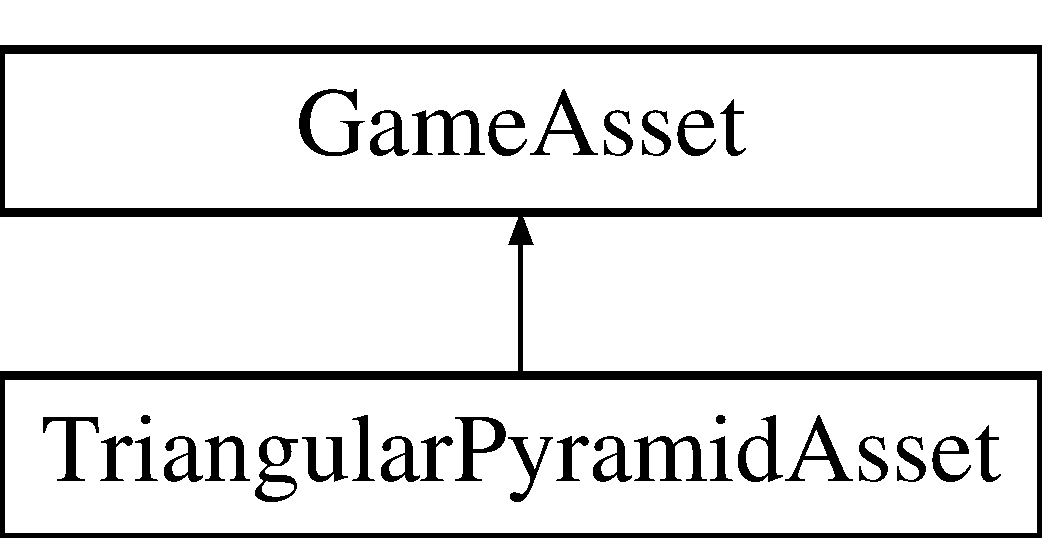
\includegraphics[height=2.000000cm]{classTriangularPyramidAsset}
\end{center}
\end{figure}
\subsection*{Public Member Functions}
\begin{DoxyCompactItemize}
\item 
\hypertarget{classTriangularPyramidAsset_a16069bd2b6fd057fb1a9a5dff1742989}{{\bfseries Triangular\-Pyramid\-Asset} (float x, float y, float z)}\label{classTriangularPyramidAsset_a16069bd2b6fd057fb1a9a5dff1742989}

\item 
virtual void \hyperlink{classTriangularPyramidAsset_a9fcab20720ad22e5e50139332b3f0190}{update} ()
\begin{DoxyCompactList}\small\item\em Update Method. \end{DoxyCompactList}\item 
virtual void \hyperlink{classTriangularPyramidAsset_a9a6c04fc73cbfc2c01477907f3033a17}{draw} ()
\begin{DoxyCompactList}\small\item\em Draw Method. \end{DoxyCompactList}\item 
\hypertarget{classTriangularPyramidAsset_a0bd9699607ea85bfde40e793ba34e142}{void {\bfseries set\-Interpolator} (shared\-\_\-ptr$<$ \hyperlink{classIInterpolator}{I\-Interpolator} $>$ li)}\label{classTriangularPyramidAsset_a0bd9699607ea85bfde40e793ba34e142}

\end{DoxyCompactItemize}
\subsection*{Additional Inherited Members}


\subsection{Detailed Description}
\hyperlink{classTriangularPyramidAsset}{Triangular\-Pyramid\-Asset} Class. 

A class to a simple triangular pyramid. 

Definition at line 19 of file Triangular\-Pyramid\-Asset.\-h.



\subsection{Member Function Documentation}
\hypertarget{classTriangularPyramidAsset_a9a6c04fc73cbfc2c01477907f3033a17}{\index{Triangular\-Pyramid\-Asset@{Triangular\-Pyramid\-Asset}!draw@{draw}}
\index{draw@{draw}!TriangularPyramidAsset@{Triangular\-Pyramid\-Asset}}
\subsubsection[{draw}]{\setlength{\rightskip}{0pt plus 5cm}void Triangular\-Pyramid\-Asset\-::draw (
\begin{DoxyParamCaption}
{}
\end{DoxyParamCaption}
)\hspace{0.3cm}{\ttfamily [virtual]}}}\label{classTriangularPyramidAsset_a9a6c04fc73cbfc2c01477907f3033a17}


Draw Method. 

Draws this asset in a 3\-D context. 

Reimplemented from \hyperlink{classGameAsset}{Game\-Asset}.



Definition at line 85 of file Triangular\-Pyramid\-Asset.\-cpp.

\hypertarget{classTriangularPyramidAsset_a9fcab20720ad22e5e50139332b3f0190}{\index{Triangular\-Pyramid\-Asset@{Triangular\-Pyramid\-Asset}!update@{update}}
\index{update@{update}!TriangularPyramidAsset@{Triangular\-Pyramid\-Asset}}
\subsubsection[{update}]{\setlength{\rightskip}{0pt plus 5cm}void Triangular\-Pyramid\-Asset\-::update (
\begin{DoxyParamCaption}
{}
\end{DoxyParamCaption}
)\hspace{0.3cm}{\ttfamily [virtual]}}}\label{classTriangularPyramidAsset_a9fcab20720ad22e5e50139332b3f0190}


Update Method. 

Updates the asset using the interpolator. 

Implements \hyperlink{classGameAsset}{Game\-Asset}.



Definition at line 71 of file Triangular\-Pyramid\-Asset.\-cpp.



The documentation for this class was generated from the following files\-:\begin{DoxyCompactItemize}
\item 
src/Triangular\-Pyramid\-Asset.\-h\item 
src/Triangular\-Pyramid\-Asset.\-cpp\end{DoxyCompactItemize}

\hypertarget{classVectormath_1_1Aos_1_1VecIdx}{\section{Vectormath\-:\-:Aos\-:\-:Vec\-Idx Class Reference}
\label{classVectormath_1_1Aos_1_1VecIdx}\index{Vectormath\-::\-Aos\-::\-Vec\-Idx@{Vectormath\-::\-Aos\-::\-Vec\-Idx}}
}
\subsection*{Public Member Functions}
\begin{DoxyCompactItemize}
\item 
\hypertarget{classVectormath_1_1Aos_1_1VecIdx_ad1b0d58575c706efba5591db93eae084}{{\bfseries Vec\-Idx} (vec\-\_\-float4\-\_\-t \&vec, int idx)}\label{classVectormath_1_1Aos_1_1VecIdx_ad1b0d58575c706efba5591db93eae084}

\item 
\hypertarget{classVectormath_1_1Aos_1_1VecIdx_a07473426600b7271c5ae484c7a907520}{{\bfseries operator float} () const }\label{classVectormath_1_1Aos_1_1VecIdx_a07473426600b7271c5ae484c7a907520}

\item 
\hypertarget{classVectormath_1_1Aos_1_1VecIdx_a58ae7653875533e2c3e7bb7a2ad03545}{float {\bfseries operator=} (float scalar)}\label{classVectormath_1_1Aos_1_1VecIdx_a58ae7653875533e2c3e7bb7a2ad03545}

\item 
\hypertarget{classVectormath_1_1Aos_1_1VecIdx_a35de28946a701698c13a5cb4dbe1289b}{\hyperlink{classVectormath_1_1floatInVec}{float\-In\-Vec} {\bfseries operator=} (\hyperlink{classVectormath_1_1floatInVec}{float\-In\-Vec} scalar)}\label{classVectormath_1_1Aos_1_1VecIdx_a35de28946a701698c13a5cb4dbe1289b}

\item 
\hypertarget{classVectormath_1_1Aos_1_1VecIdx_a907abfa83bed3474ad8b4b609a5d7783}{\hyperlink{classVectormath_1_1floatInVec}{float\-In\-Vec} {\bfseries operator=} (const \hyperlink{classVectormath_1_1Aos_1_1VecIdx}{Vec\-Idx} \&scalar)}\label{classVectormath_1_1Aos_1_1VecIdx_a907abfa83bed3474ad8b4b609a5d7783}

\item 
\hypertarget{classVectormath_1_1Aos_1_1VecIdx_ae82c6bf1b95a08d93061b0604b2d91eb}{\hyperlink{classVectormath_1_1floatInVec}{float\-In\-Vec} {\bfseries operator$\ast$=} (float scalar)}\label{classVectormath_1_1Aos_1_1VecIdx_ae82c6bf1b95a08d93061b0604b2d91eb}

\item 
\hypertarget{classVectormath_1_1Aos_1_1VecIdx_a35fb35124b8ee48f40e6ff3488938f3e}{\hyperlink{classVectormath_1_1floatInVec}{float\-In\-Vec} {\bfseries operator$\ast$=} (\hyperlink{classVectormath_1_1floatInVec}{float\-In\-Vec} scalar)}\label{classVectormath_1_1Aos_1_1VecIdx_a35fb35124b8ee48f40e6ff3488938f3e}

\item 
\hypertarget{classVectormath_1_1Aos_1_1VecIdx_aa019cd8914ee62998de25119b3eaeddf}{\hyperlink{classVectormath_1_1floatInVec}{float\-In\-Vec} {\bfseries operator/=} (float scalar)}\label{classVectormath_1_1Aos_1_1VecIdx_aa019cd8914ee62998de25119b3eaeddf}

\item 
\hypertarget{classVectormath_1_1Aos_1_1VecIdx_ab9191a40f975e4d22a1e011bc5e17148}{\hyperlink{classVectormath_1_1floatInVec}{float\-In\-Vec} {\bfseries operator/=} (\hyperlink{classVectormath_1_1floatInVec}{float\-In\-Vec} scalar)}\label{classVectormath_1_1Aos_1_1VecIdx_ab9191a40f975e4d22a1e011bc5e17148}

\item 
\hypertarget{classVectormath_1_1Aos_1_1VecIdx_ae62579d054d509654be2a2088587db70}{\hyperlink{classVectormath_1_1floatInVec}{float\-In\-Vec} {\bfseries operator+=} (float scalar)}\label{classVectormath_1_1Aos_1_1VecIdx_ae62579d054d509654be2a2088587db70}

\item 
\hypertarget{classVectormath_1_1Aos_1_1VecIdx_ae92479927205286e0666396b9da5395d}{\hyperlink{classVectormath_1_1floatInVec}{float\-In\-Vec} {\bfseries operator+=} (\hyperlink{classVectormath_1_1floatInVec}{float\-In\-Vec} scalar)}\label{classVectormath_1_1Aos_1_1VecIdx_ae92479927205286e0666396b9da5395d}

\item 
\hypertarget{classVectormath_1_1Aos_1_1VecIdx_a761d84eee7847ad7149b399780d36167}{\hyperlink{classVectormath_1_1floatInVec}{float\-In\-Vec} {\bfseries operator-\/=} (float scalar)}\label{classVectormath_1_1Aos_1_1VecIdx_a761d84eee7847ad7149b399780d36167}

\item 
\hypertarget{classVectormath_1_1Aos_1_1VecIdx_a67691e4a230b9cdf4f8f9846fc01f01f}{\hyperlink{classVectormath_1_1floatInVec}{float\-In\-Vec} {\bfseries operator-\/=} (\hyperlink{classVectormath_1_1floatInVec}{float\-In\-Vec} scalar)}\label{classVectormath_1_1Aos_1_1VecIdx_a67691e4a230b9cdf4f8f9846fc01f01f}

\item 
\hypertarget{classVectormath_1_1Aos_1_1VecIdx_a8e40b884277e9421e294f5906e7452e8}{{\bfseries Vec\-Idx} (vec\-\_\-float4 \&vec, int idx)}\label{classVectormath_1_1Aos_1_1VecIdx_a8e40b884277e9421e294f5906e7452e8}

\item 
\hypertarget{classVectormath_1_1Aos_1_1VecIdx_aecba0ac0fdaea640cb3c373eb21cfdda}{{\bfseries operator float} () const }\label{classVectormath_1_1Aos_1_1VecIdx_aecba0ac0fdaea640cb3c373eb21cfdda}

\item 
\hypertarget{classVectormath_1_1Aos_1_1VecIdx_a2900ce64010206c5eb676f6c9338adbd}{float {\bfseries operator=} (float scalar)}\label{classVectormath_1_1Aos_1_1VecIdx_a2900ce64010206c5eb676f6c9338adbd}

\item 
\hypertarget{classVectormath_1_1Aos_1_1VecIdx_afcd2bedac1ae7f5b7549accb77f3edbc}{float {\bfseries operator=} (const \hyperlink{classVectormath_1_1Aos_1_1VecIdx}{Vec\-Idx} \&scalar)}\label{classVectormath_1_1Aos_1_1VecIdx_afcd2bedac1ae7f5b7549accb77f3edbc}

\item 
\hypertarget{classVectormath_1_1Aos_1_1VecIdx_aac958ef606b0f2c185f3713bf5649ddc}{float {\bfseries operator$\ast$=} (float scalar)}\label{classVectormath_1_1Aos_1_1VecIdx_aac958ef606b0f2c185f3713bf5649ddc}

\item 
\hypertarget{classVectormath_1_1Aos_1_1VecIdx_a6f435d5924a565ec2a04949778d47ca6}{float {\bfseries operator/=} (float scalar)}\label{classVectormath_1_1Aos_1_1VecIdx_a6f435d5924a565ec2a04949778d47ca6}

\item 
\hypertarget{classVectormath_1_1Aos_1_1VecIdx_a9c2012ddcb1884faba437e6f8950ed7d}{float {\bfseries operator+=} (float scalar)}\label{classVectormath_1_1Aos_1_1VecIdx_a9c2012ddcb1884faba437e6f8950ed7d}

\item 
\hypertarget{classVectormath_1_1Aos_1_1VecIdx_a97233d2ad8b81b3741f8d59ac61d427d}{float {\bfseries operator-\/=} (float scalar)}\label{classVectormath_1_1Aos_1_1VecIdx_a97233d2ad8b81b3741f8d59ac61d427d}

\end{DoxyCompactItemize}


\subsection{Detailed Description}


Definition at line 44 of file vecidx\-\_\-aos.\-h.



The documentation for this class was generated from the following files\-:\begin{DoxyCompactItemize}
\item 
src/include/vectormath/ppu/cpp/vecidx\-\_\-aos.\-h\item 
src/include/vectormath/ppu/cpp/vec\-\_\-aos.\-h\end{DoxyCompactItemize}

\hypertarget{classVectormath_1_1Soa_1_1Vector3}{\section{Vectormath\-:\-:Soa\-:\-:Vector3 Class Reference}
\label{classVectormath_1_1Soa_1_1Vector3}\index{Vectormath\-::\-Soa\-::\-Vector3@{Vectormath\-::\-Soa\-::\-Vector3}}
}
\subsection*{Public Member Functions}
\begin{DoxyCompactItemize}
\item 
\hypertarget{classVectormath_1_1Soa_1_1Vector3_adae211af29e368313024b74f9db3df91}{{\bfseries Vector3} (const \hyperlink{classVectormath_1_1Soa_1_1Vector3}{Vector3} \&vec)}\label{classVectormath_1_1Soa_1_1Vector3_adae211af29e368313024b74f9db3df91}

\item 
\hypertarget{classVectormath_1_1Soa_1_1Vector3_a9b6c2c9ca162b4a67a126a6f39a2fcf3}{{\bfseries Vector3} (vec\-\_\-float4 x, vec\-\_\-float4 y, vec\-\_\-float4 z)}\label{classVectormath_1_1Soa_1_1Vector3_a9b6c2c9ca162b4a67a126a6f39a2fcf3}

\item 
\hypertarget{classVectormath_1_1Soa_1_1Vector3_adfa1eab885896c70eef4cc43d2b70976}{{\bfseries Vector3} (const \hyperlink{classVectormath_1_1Soa_1_1Point3}{Point3} \&pnt)}\label{classVectormath_1_1Soa_1_1Vector3_adfa1eab885896c70eef4cc43d2b70976}

\item 
\hypertarget{classVectormath_1_1Soa_1_1Vector3_a007123be368a50e520e8201e53b5f028}{{\bfseries Vector3} (vec\-\_\-float4 scalar)}\label{classVectormath_1_1Soa_1_1Vector3_a007123be368a50e520e8201e53b5f028}

\item 
\hypertarget{classVectormath_1_1Soa_1_1Vector3_a4bed8595f3c35e6cc85434308b6e7a11}{{\bfseries Vector3} (\hyperlink{classVectormath_1_1Aos_1_1Vector3}{Aos\-::\-Vector3} vec)}\label{classVectormath_1_1Soa_1_1Vector3_a4bed8595f3c35e6cc85434308b6e7a11}

\item 
\hypertarget{classVectormath_1_1Soa_1_1Vector3_a8745c2b774b896367f1344c002926a17}{{\bfseries Vector3} (\hyperlink{classVectormath_1_1Aos_1_1Vector3}{Aos\-::\-Vector3} vec0, \hyperlink{classVectormath_1_1Aos_1_1Vector3}{Aos\-::\-Vector3} vec1, \hyperlink{classVectormath_1_1Aos_1_1Vector3}{Aos\-::\-Vector3} vec2, \hyperlink{classVectormath_1_1Aos_1_1Vector3}{Aos\-::\-Vector3} vec3)}\label{classVectormath_1_1Soa_1_1Vector3_a8745c2b774b896367f1344c002926a17}

\item 
\hypertarget{classVectormath_1_1Soa_1_1Vector3_a324c1d0d4bb3d5d6e42ec7dde14363e1}{void {\bfseries get4\-Aos} (\hyperlink{classVectormath_1_1Aos_1_1Vector3}{Aos\-::\-Vector3} \&result0, \hyperlink{classVectormath_1_1Aos_1_1Vector3}{Aos\-::\-Vector3} \&result1, \hyperlink{classVectormath_1_1Aos_1_1Vector3}{Aos\-::\-Vector3} \&result2, \hyperlink{classVectormath_1_1Aos_1_1Vector3}{Aos\-::\-Vector3} \&result3) const }\label{classVectormath_1_1Soa_1_1Vector3_a324c1d0d4bb3d5d6e42ec7dde14363e1}

\item 
\hypertarget{classVectormath_1_1Soa_1_1Vector3_a034e9a948f111085b382127f8f8e34e4}{\hyperlink{classVectormath_1_1Soa_1_1Vector3}{Vector3} \& {\bfseries operator=} (const \hyperlink{classVectormath_1_1Soa_1_1Vector3}{Vector3} \&vec)}\label{classVectormath_1_1Soa_1_1Vector3_a034e9a948f111085b382127f8f8e34e4}

\item 
\hypertarget{classVectormath_1_1Soa_1_1Vector3_a0dfaabb000ed186ad2e36665eda9ce0b}{\hyperlink{classVectormath_1_1Soa_1_1Vector3}{Vector3} \& {\bfseries set\-X} (vec\-\_\-float4 x)}\label{classVectormath_1_1Soa_1_1Vector3_a0dfaabb000ed186ad2e36665eda9ce0b}

\item 
\hypertarget{classVectormath_1_1Soa_1_1Vector3_ae098e41f5f57eb4a5f871e6d6d77c26d}{\hyperlink{classVectormath_1_1Soa_1_1Vector3}{Vector3} \& {\bfseries set\-Y} (vec\-\_\-float4 y)}\label{classVectormath_1_1Soa_1_1Vector3_ae098e41f5f57eb4a5f871e6d6d77c26d}

\item 
\hypertarget{classVectormath_1_1Soa_1_1Vector3_a603cf94e5585cf9352a9b31be491f3e4}{\hyperlink{classVectormath_1_1Soa_1_1Vector3}{Vector3} \& {\bfseries set\-Z} (vec\-\_\-float4 z)}\label{classVectormath_1_1Soa_1_1Vector3_a603cf94e5585cf9352a9b31be491f3e4}

\item 
\hypertarget{classVectormath_1_1Soa_1_1Vector3_a2f6157ae5a1db067e5f3f0790a824730}{vec\-\_\-float4 {\bfseries get\-X} () const }\label{classVectormath_1_1Soa_1_1Vector3_a2f6157ae5a1db067e5f3f0790a824730}

\item 
\hypertarget{classVectormath_1_1Soa_1_1Vector3_a4776125d80723b46e9be7ce8eb931f8f}{vec\-\_\-float4 {\bfseries get\-Y} () const }\label{classVectormath_1_1Soa_1_1Vector3_a4776125d80723b46e9be7ce8eb931f8f}

\item 
\hypertarget{classVectormath_1_1Soa_1_1Vector3_a7e2c50267eb7a53732851c1dde6e35c3}{vec\-\_\-float4 {\bfseries get\-Z} () const }\label{classVectormath_1_1Soa_1_1Vector3_a7e2c50267eb7a53732851c1dde6e35c3}

\item 
\hypertarget{classVectormath_1_1Soa_1_1Vector3_a832370b209da6d5a51b1e3951e691e03}{\hyperlink{classVectormath_1_1Soa_1_1Vector3}{Vector3} \& {\bfseries set\-Elem} (int idx, vec\-\_\-float4 value)}\label{classVectormath_1_1Soa_1_1Vector3_a832370b209da6d5a51b1e3951e691e03}

\item 
\hypertarget{classVectormath_1_1Soa_1_1Vector3_a292769e6a081ad3e0ed926f367e388cb}{vec\-\_\-float4 {\bfseries get\-Elem} (int idx) const }\label{classVectormath_1_1Soa_1_1Vector3_a292769e6a081ad3e0ed926f367e388cb}

\item 
\hypertarget{classVectormath_1_1Soa_1_1Vector3_a2941b034b91f29398b8049d1c88e93ba}{vec\-\_\-float4\-\_\-t \& {\bfseries operator\mbox{[}$\,$\mbox{]}} (int idx)}\label{classVectormath_1_1Soa_1_1Vector3_a2941b034b91f29398b8049d1c88e93ba}

\item 
\hypertarget{classVectormath_1_1Soa_1_1Vector3_a2fc951153b4eb4972fe66a717991c4ec}{vec\-\_\-float4 {\bfseries operator\mbox{[}$\,$\mbox{]}} (int idx) const }\label{classVectormath_1_1Soa_1_1Vector3_a2fc951153b4eb4972fe66a717991c4ec}

\item 
\hypertarget{classVectormath_1_1Soa_1_1Vector3_a25248c9d703b6b2f4465fd000649300a}{const \hyperlink{classVectormath_1_1Soa_1_1Vector3}{Vector3} {\bfseries operator+} (const \hyperlink{classVectormath_1_1Soa_1_1Vector3}{Vector3} \&vec) const }\label{classVectormath_1_1Soa_1_1Vector3_a25248c9d703b6b2f4465fd000649300a}

\item 
\hypertarget{classVectormath_1_1Soa_1_1Vector3_a959f535529253b73cfbe663e6398cea6}{const \hyperlink{classVectormath_1_1Soa_1_1Vector3}{Vector3} {\bfseries operator-\/} (const \hyperlink{classVectormath_1_1Soa_1_1Vector3}{Vector3} \&vec) const }\label{classVectormath_1_1Soa_1_1Vector3_a959f535529253b73cfbe663e6398cea6}

\item 
\hypertarget{classVectormath_1_1Soa_1_1Vector3_aa20972188526c5f28733f0e4df204a0c}{const \hyperlink{classVectormath_1_1Soa_1_1Point3}{Point3} {\bfseries operator+} (const \hyperlink{classVectormath_1_1Soa_1_1Point3}{Point3} \&pnt) const }\label{classVectormath_1_1Soa_1_1Vector3_aa20972188526c5f28733f0e4df204a0c}

\item 
\hypertarget{classVectormath_1_1Soa_1_1Vector3_a85772c027223a9cd7b6f1727202a356e}{const \hyperlink{classVectormath_1_1Soa_1_1Vector3}{Vector3} {\bfseries operator$\ast$} (vec\-\_\-float4 scalar) const }\label{classVectormath_1_1Soa_1_1Vector3_a85772c027223a9cd7b6f1727202a356e}

\item 
\hypertarget{classVectormath_1_1Soa_1_1Vector3_a08222130d6aa192a3b0026ae827dfe01}{const \hyperlink{classVectormath_1_1Soa_1_1Vector3}{Vector3} {\bfseries operator/} (vec\-\_\-float4 scalar) const }\label{classVectormath_1_1Soa_1_1Vector3_a08222130d6aa192a3b0026ae827dfe01}

\item 
\hypertarget{classVectormath_1_1Soa_1_1Vector3_ad0c93ef1232f6dce5a0fb911d664c9da}{\hyperlink{classVectormath_1_1Soa_1_1Vector3}{Vector3} \& {\bfseries operator+=} (const \hyperlink{classVectormath_1_1Soa_1_1Vector3}{Vector3} \&vec)}\label{classVectormath_1_1Soa_1_1Vector3_ad0c93ef1232f6dce5a0fb911d664c9da}

\item 
\hypertarget{classVectormath_1_1Soa_1_1Vector3_a50992d7cdf70db9f0250d338a045d025}{\hyperlink{classVectormath_1_1Soa_1_1Vector3}{Vector3} \& {\bfseries operator-\/=} (const \hyperlink{classVectormath_1_1Soa_1_1Vector3}{Vector3} \&vec)}\label{classVectormath_1_1Soa_1_1Vector3_a50992d7cdf70db9f0250d338a045d025}

\item 
\hypertarget{classVectormath_1_1Soa_1_1Vector3_a6ffe494305ca17296a96d9fc5b7231a5}{\hyperlink{classVectormath_1_1Soa_1_1Vector3}{Vector3} \& {\bfseries operator$\ast$=} (vec\-\_\-float4 scalar)}\label{classVectormath_1_1Soa_1_1Vector3_a6ffe494305ca17296a96d9fc5b7231a5}

\item 
\hypertarget{classVectormath_1_1Soa_1_1Vector3_a33aaff03e5c85d1be4093fa1e2dfbef0}{\hyperlink{classVectormath_1_1Soa_1_1Vector3}{Vector3} \& {\bfseries operator/=} (vec\-\_\-float4 scalar)}\label{classVectormath_1_1Soa_1_1Vector3_a33aaff03e5c85d1be4093fa1e2dfbef0}

\item 
\hypertarget{classVectormath_1_1Soa_1_1Vector3_a7ffc33c34936fd010ad560a7f94c27f5}{const \hyperlink{classVectormath_1_1Soa_1_1Vector3}{Vector3} {\bfseries operator-\/} () const }\label{classVectormath_1_1Soa_1_1Vector3_a7ffc33c34936fd010ad560a7f94c27f5}

\item 
\hypertarget{classVectormath_1_1Soa_1_1Vector3_adae211af29e368313024b74f9db3df91}{{\bfseries Vector3} (const \hyperlink{classVectormath_1_1Soa_1_1Vector3}{Vector3} \&vec)}\label{classVectormath_1_1Soa_1_1Vector3_adae211af29e368313024b74f9db3df91}

\item 
\hypertarget{classVectormath_1_1Soa_1_1Vector3_a9b6c2c9ca162b4a67a126a6f39a2fcf3}{{\bfseries Vector3} (vec\-\_\-float4 x, vec\-\_\-float4 y, vec\-\_\-float4 z)}\label{classVectormath_1_1Soa_1_1Vector3_a9b6c2c9ca162b4a67a126a6f39a2fcf3}

\item 
\hypertarget{classVectormath_1_1Soa_1_1Vector3_adfa1eab885896c70eef4cc43d2b70976}{{\bfseries Vector3} (const \hyperlink{classVectormath_1_1Soa_1_1Point3}{Point3} \&pnt)}\label{classVectormath_1_1Soa_1_1Vector3_adfa1eab885896c70eef4cc43d2b70976}

\item 
\hypertarget{classVectormath_1_1Soa_1_1Vector3_a007123be368a50e520e8201e53b5f028}{{\bfseries Vector3} (vec\-\_\-float4 scalar)}\label{classVectormath_1_1Soa_1_1Vector3_a007123be368a50e520e8201e53b5f028}

\item 
\hypertarget{classVectormath_1_1Soa_1_1Vector3_a4bed8595f3c35e6cc85434308b6e7a11}{{\bfseries Vector3} (\hyperlink{classVectormath_1_1Aos_1_1Vector3}{Aos\-::\-Vector3} vec)}\label{classVectormath_1_1Soa_1_1Vector3_a4bed8595f3c35e6cc85434308b6e7a11}

\item 
\hypertarget{classVectormath_1_1Soa_1_1Vector3_a8745c2b774b896367f1344c002926a17}{{\bfseries Vector3} (\hyperlink{classVectormath_1_1Aos_1_1Vector3}{Aos\-::\-Vector3} vec0, \hyperlink{classVectormath_1_1Aos_1_1Vector3}{Aos\-::\-Vector3} vec1, \hyperlink{classVectormath_1_1Aos_1_1Vector3}{Aos\-::\-Vector3} vec2, \hyperlink{classVectormath_1_1Aos_1_1Vector3}{Aos\-::\-Vector3} vec3)}\label{classVectormath_1_1Soa_1_1Vector3_a8745c2b774b896367f1344c002926a17}

\item 
\hypertarget{classVectormath_1_1Soa_1_1Vector3_a324c1d0d4bb3d5d6e42ec7dde14363e1}{void {\bfseries get4\-Aos} (\hyperlink{classVectormath_1_1Aos_1_1Vector3}{Aos\-::\-Vector3} \&result0, \hyperlink{classVectormath_1_1Aos_1_1Vector3}{Aos\-::\-Vector3} \&result1, \hyperlink{classVectormath_1_1Aos_1_1Vector3}{Aos\-::\-Vector3} \&result2, \hyperlink{classVectormath_1_1Aos_1_1Vector3}{Aos\-::\-Vector3} \&result3) const }\label{classVectormath_1_1Soa_1_1Vector3_a324c1d0d4bb3d5d6e42ec7dde14363e1}

\item 
\hypertarget{classVectormath_1_1Soa_1_1Vector3_a39d3cbe6129d6f252d5074b4e7daa50a}{\hyperlink{classVectormath_1_1Soa_1_1Vector3}{Vector3} \& {\bfseries operator=} (const \hyperlink{classVectormath_1_1Soa_1_1Vector3}{Vector3} \&vec)}\label{classVectormath_1_1Soa_1_1Vector3_a39d3cbe6129d6f252d5074b4e7daa50a}

\item 
\hypertarget{classVectormath_1_1Soa_1_1Vector3_abb6e88df34d361535c9a1e234873df7b}{\hyperlink{classVectormath_1_1Soa_1_1Vector3}{Vector3} \& {\bfseries set\-X} (vec\-\_\-float4 x)}\label{classVectormath_1_1Soa_1_1Vector3_abb6e88df34d361535c9a1e234873df7b}

\item 
\hypertarget{classVectormath_1_1Soa_1_1Vector3_a065047f20c745328f8b992d4ce64ad61}{\hyperlink{classVectormath_1_1Soa_1_1Vector3}{Vector3} \& {\bfseries set\-Y} (vec\-\_\-float4 y)}\label{classVectormath_1_1Soa_1_1Vector3_a065047f20c745328f8b992d4ce64ad61}

\item 
\hypertarget{classVectormath_1_1Soa_1_1Vector3_a3c806f40fcdc3a69e16a5c673063b98a}{\hyperlink{classVectormath_1_1Soa_1_1Vector3}{Vector3} \& {\bfseries set\-Z} (vec\-\_\-float4 z)}\label{classVectormath_1_1Soa_1_1Vector3_a3c806f40fcdc3a69e16a5c673063b98a}

\item 
\hypertarget{classVectormath_1_1Soa_1_1Vector3_a2f6157ae5a1db067e5f3f0790a824730}{vec\-\_\-float4 {\bfseries get\-X} () const }\label{classVectormath_1_1Soa_1_1Vector3_a2f6157ae5a1db067e5f3f0790a824730}

\item 
\hypertarget{classVectormath_1_1Soa_1_1Vector3_a4776125d80723b46e9be7ce8eb931f8f}{vec\-\_\-float4 {\bfseries get\-Y} () const }\label{classVectormath_1_1Soa_1_1Vector3_a4776125d80723b46e9be7ce8eb931f8f}

\item 
\hypertarget{classVectormath_1_1Soa_1_1Vector3_a7e2c50267eb7a53732851c1dde6e35c3}{vec\-\_\-float4 {\bfseries get\-Z} () const }\label{classVectormath_1_1Soa_1_1Vector3_a7e2c50267eb7a53732851c1dde6e35c3}

\item 
\hypertarget{classVectormath_1_1Soa_1_1Vector3_a2891eb3f05d1ef37fbee4f816d50b46c}{\hyperlink{classVectormath_1_1Soa_1_1Vector3}{Vector3} \& {\bfseries set\-Elem} (int idx, vec\-\_\-float4 value)}\label{classVectormath_1_1Soa_1_1Vector3_a2891eb3f05d1ef37fbee4f816d50b46c}

\item 
\hypertarget{classVectormath_1_1Soa_1_1Vector3_a292769e6a081ad3e0ed926f367e388cb}{vec\-\_\-float4 {\bfseries get\-Elem} (int idx) const }\label{classVectormath_1_1Soa_1_1Vector3_a292769e6a081ad3e0ed926f367e388cb}

\item 
\hypertarget{classVectormath_1_1Soa_1_1Vector3_af2dc0b0d5a92dc580591461085b5a5f8}{vec\-\_\-float4\-\_\-t \& {\bfseries operator\mbox{[}$\,$\mbox{]}} (int idx)}\label{classVectormath_1_1Soa_1_1Vector3_af2dc0b0d5a92dc580591461085b5a5f8}

\item 
\hypertarget{classVectormath_1_1Soa_1_1Vector3_a2fc951153b4eb4972fe66a717991c4ec}{vec\-\_\-float4 {\bfseries operator\mbox{[}$\,$\mbox{]}} (int idx) const }\label{classVectormath_1_1Soa_1_1Vector3_a2fc951153b4eb4972fe66a717991c4ec}

\item 
\hypertarget{classVectormath_1_1Soa_1_1Vector3_a25248c9d703b6b2f4465fd000649300a}{const \hyperlink{classVectormath_1_1Soa_1_1Vector3}{Vector3} {\bfseries operator+} (const \hyperlink{classVectormath_1_1Soa_1_1Vector3}{Vector3} \&vec) const }\label{classVectormath_1_1Soa_1_1Vector3_a25248c9d703b6b2f4465fd000649300a}

\item 
\hypertarget{classVectormath_1_1Soa_1_1Vector3_a959f535529253b73cfbe663e6398cea6}{const \hyperlink{classVectormath_1_1Soa_1_1Vector3}{Vector3} {\bfseries operator-\/} (const \hyperlink{classVectormath_1_1Soa_1_1Vector3}{Vector3} \&vec) const }\label{classVectormath_1_1Soa_1_1Vector3_a959f535529253b73cfbe663e6398cea6}

\item 
\hypertarget{classVectormath_1_1Soa_1_1Vector3_aa20972188526c5f28733f0e4df204a0c}{const \hyperlink{classVectormath_1_1Soa_1_1Point3}{Point3} {\bfseries operator+} (const \hyperlink{classVectormath_1_1Soa_1_1Point3}{Point3} \&pnt) const }\label{classVectormath_1_1Soa_1_1Vector3_aa20972188526c5f28733f0e4df204a0c}

\item 
\hypertarget{classVectormath_1_1Soa_1_1Vector3_a85772c027223a9cd7b6f1727202a356e}{const \hyperlink{classVectormath_1_1Soa_1_1Vector3}{Vector3} {\bfseries operator$\ast$} (vec\-\_\-float4 scalar) const }\label{classVectormath_1_1Soa_1_1Vector3_a85772c027223a9cd7b6f1727202a356e}

\item 
\hypertarget{classVectormath_1_1Soa_1_1Vector3_a08222130d6aa192a3b0026ae827dfe01}{const \hyperlink{classVectormath_1_1Soa_1_1Vector3}{Vector3} {\bfseries operator/} (vec\-\_\-float4 scalar) const }\label{classVectormath_1_1Soa_1_1Vector3_a08222130d6aa192a3b0026ae827dfe01}

\item 
\hypertarget{classVectormath_1_1Soa_1_1Vector3_a7aa0b348828f87b41a11f4b6f779f062}{\hyperlink{classVectormath_1_1Soa_1_1Vector3}{Vector3} \& {\bfseries operator+=} (const \hyperlink{classVectormath_1_1Soa_1_1Vector3}{Vector3} \&vec)}\label{classVectormath_1_1Soa_1_1Vector3_a7aa0b348828f87b41a11f4b6f779f062}

\item 
\hypertarget{classVectormath_1_1Soa_1_1Vector3_afd804671c3d8d7d6cc52e67945e8e943}{\hyperlink{classVectormath_1_1Soa_1_1Vector3}{Vector3} \& {\bfseries operator-\/=} (const \hyperlink{classVectormath_1_1Soa_1_1Vector3}{Vector3} \&vec)}\label{classVectormath_1_1Soa_1_1Vector3_afd804671c3d8d7d6cc52e67945e8e943}

\item 
\hypertarget{classVectormath_1_1Soa_1_1Vector3_a35d3c251efcaa2d4d497a88ee70e14da}{\hyperlink{classVectormath_1_1Soa_1_1Vector3}{Vector3} \& {\bfseries operator$\ast$=} (vec\-\_\-float4 scalar)}\label{classVectormath_1_1Soa_1_1Vector3_a35d3c251efcaa2d4d497a88ee70e14da}

\item 
\hypertarget{classVectormath_1_1Soa_1_1Vector3_a6b47a68ae5013a1fb4d456a145325e08}{\hyperlink{classVectormath_1_1Soa_1_1Vector3}{Vector3} \& {\bfseries operator/=} (vec\-\_\-float4 scalar)}\label{classVectormath_1_1Soa_1_1Vector3_a6b47a68ae5013a1fb4d456a145325e08}

\item 
\hypertarget{classVectormath_1_1Soa_1_1Vector3_a7ffc33c34936fd010ad560a7f94c27f5}{const \hyperlink{classVectormath_1_1Soa_1_1Vector3}{Vector3} {\bfseries operator-\/} () const }\label{classVectormath_1_1Soa_1_1Vector3_a7ffc33c34936fd010ad560a7f94c27f5}

\end{DoxyCompactItemize}
\subsection*{Static Public Member Functions}
\begin{DoxyCompactItemize}
\item 
\hypertarget{classVectormath_1_1Soa_1_1Vector3_a73a285c366ee9d0ad110e62c87ad6d8d}{static const \hyperlink{classVectormath_1_1Soa_1_1Vector3}{Vector3} {\bfseries x\-Axis} ()}\label{classVectormath_1_1Soa_1_1Vector3_a73a285c366ee9d0ad110e62c87ad6d8d}

\item 
\hypertarget{classVectormath_1_1Soa_1_1Vector3_a16bb85c1f9c33861fa10ddc16ad85b85}{static const \hyperlink{classVectormath_1_1Soa_1_1Vector3}{Vector3} {\bfseries y\-Axis} ()}\label{classVectormath_1_1Soa_1_1Vector3_a16bb85c1f9c33861fa10ddc16ad85b85}

\item 
\hypertarget{classVectormath_1_1Soa_1_1Vector3_a161faad15f0e3a73b22c400f5edefc12}{static const \hyperlink{classVectormath_1_1Soa_1_1Vector3}{Vector3} {\bfseries z\-Axis} ()}\label{classVectormath_1_1Soa_1_1Vector3_a161faad15f0e3a73b22c400f5edefc12}

\item 
\hypertarget{classVectormath_1_1Soa_1_1Vector3_a152564d7413e60b5633d964512307628}{static const \hyperlink{classVectormath_1_1Soa_1_1Vector3}{Vector3} {\bfseries x\-Axis} ()}\label{classVectormath_1_1Soa_1_1Vector3_a152564d7413e60b5633d964512307628}

\item 
\hypertarget{classVectormath_1_1Soa_1_1Vector3_ad24024937de752e0468fc5487deaeae6}{static const \hyperlink{classVectormath_1_1Soa_1_1Vector3}{Vector3} {\bfseries y\-Axis} ()}\label{classVectormath_1_1Soa_1_1Vector3_ad24024937de752e0468fc5487deaeae6}

\item 
\hypertarget{classVectormath_1_1Soa_1_1Vector3_adbad8f188a7e8015e9f3a12bcd0c34fb}{static const \hyperlink{classVectormath_1_1Soa_1_1Vector3}{Vector3} {\bfseries z\-Axis} ()}\label{classVectormath_1_1Soa_1_1Vector3_adbad8f188a7e8015e9f3a12bcd0c34fb}

\end{DoxyCompactItemize}


\subsection{Detailed Description}


Definition at line 59 of file vectormath\-\_\-soa.\-h.



The documentation for this class was generated from the following files\-:\begin{DoxyCompactItemize}
\item 
src/include/vectormath/ppu/cpp/vectormath\-\_\-soa.\-h\item 
src/include/vectormath/ppu/cpp/vec\-\_\-soa.\-h\end{DoxyCompactItemize}

\hypertarget{classVectormath_1_1Aos_1_1Vector3}{\section{Vectormath\-:\-:Aos\-:\-:Vector3 Class Reference}
\label{classVectormath_1_1Aos_1_1Vector3}\index{Vectormath\-::\-Aos\-::\-Vector3@{Vectormath\-::\-Aos\-::\-Vector3}}
}
\subsection*{Public Member Functions}
\begin{DoxyCompactItemize}
\item 
\hypertarget{classVectormath_1_1Aos_1_1Vector3_afdc94668060aaeb330502e69aa6d7a74}{{\bfseries Vector3} (float x, float y, float z)}\label{classVectormath_1_1Aos_1_1Vector3_afdc94668060aaeb330502e69aa6d7a74}

\item 
\hypertarget{classVectormath_1_1Aos_1_1Vector3_a2925f345e01372e3a4fc90aca945dd67}{{\bfseries Vector3} (\hyperlink{classVectormath_1_1floatInVec}{float\-In\-Vec} x, \hyperlink{classVectormath_1_1floatInVec}{float\-In\-Vec} y, \hyperlink{classVectormath_1_1floatInVec}{float\-In\-Vec} z)}\label{classVectormath_1_1Aos_1_1Vector3_a2925f345e01372e3a4fc90aca945dd67}

\item 
\hypertarget{classVectormath_1_1Aos_1_1Vector3_aca6f628c50eb4eee21a5ce80b7acf585}{{\bfseries Vector3} (\hyperlink{classVectormath_1_1Aos_1_1Point3}{Point3} pnt)}\label{classVectormath_1_1Aos_1_1Vector3_aca6f628c50eb4eee21a5ce80b7acf585}

\item 
\hypertarget{classVectormath_1_1Aos_1_1Vector3_a71c6e33bbbd6cd3e3c93b08f3f29abb0}{{\bfseries Vector3} (float scalar)}\label{classVectormath_1_1Aos_1_1Vector3_a71c6e33bbbd6cd3e3c93b08f3f29abb0}

\item 
\hypertarget{classVectormath_1_1Aos_1_1Vector3_a1a6f7f54e58f1746d91b7c59a8821c4b}{{\bfseries Vector3} (\hyperlink{classVectormath_1_1floatInVec}{float\-In\-Vec} scalar)}\label{classVectormath_1_1Aos_1_1Vector3_a1a6f7f54e58f1746d91b7c59a8821c4b}

\item 
\hypertarget{classVectormath_1_1Aos_1_1Vector3_a9aaee015c69771b0e9773ced0b5d1b6b}{{\bfseries Vector3} (vec\-\_\-float4 vf4)}\label{classVectormath_1_1Aos_1_1Vector3_a9aaee015c69771b0e9773ced0b5d1b6b}

\item 
\hypertarget{classVectormath_1_1Aos_1_1Vector3_acd4ea69340ca89b06f65fc6713ebefa1}{vec\-\_\-float4 {\bfseries get128} () const }\label{classVectormath_1_1Aos_1_1Vector3_acd4ea69340ca89b06f65fc6713ebefa1}

\item 
\hypertarget{classVectormath_1_1Aos_1_1Vector3_a825e0e3ee2a149e56b56964010c8a906}{\hyperlink{classVectormath_1_1Aos_1_1Vector3}{Vector3} \& {\bfseries operator=} (\hyperlink{classVectormath_1_1Aos_1_1Vector3}{Vector3} vec)}\label{classVectormath_1_1Aos_1_1Vector3_a825e0e3ee2a149e56b56964010c8a906}

\item 
\hypertarget{classVectormath_1_1Aos_1_1Vector3_ac87395cfe312e4b2854ca49b2fe17088}{\hyperlink{classVectormath_1_1Aos_1_1Vector3}{Vector3} \& {\bfseries set\-X} (float x)}\label{classVectormath_1_1Aos_1_1Vector3_ac87395cfe312e4b2854ca49b2fe17088}

\item 
\hypertarget{classVectormath_1_1Aos_1_1Vector3_a3e01341c380e274c6b20b292d0aa9f04}{\hyperlink{classVectormath_1_1Aos_1_1Vector3}{Vector3} \& {\bfseries set\-Y} (float y)}\label{classVectormath_1_1Aos_1_1Vector3_a3e01341c380e274c6b20b292d0aa9f04}

\item 
\hypertarget{classVectormath_1_1Aos_1_1Vector3_a78fbbff95c6a56f63b024bb032e19db3}{\hyperlink{classVectormath_1_1Aos_1_1Vector3}{Vector3} \& {\bfseries set\-Z} (float z)}\label{classVectormath_1_1Aos_1_1Vector3_a78fbbff95c6a56f63b024bb032e19db3}

\item 
\hypertarget{classVectormath_1_1Aos_1_1Vector3_a80b470657ececfe777e80ebc71cf92a6}{\hyperlink{classVectormath_1_1Aos_1_1Vector3}{Vector3} \& {\bfseries set\-X} (\hyperlink{classVectormath_1_1floatInVec}{float\-In\-Vec} x)}\label{classVectormath_1_1Aos_1_1Vector3_a80b470657ececfe777e80ebc71cf92a6}

\item 
\hypertarget{classVectormath_1_1Aos_1_1Vector3_abc8a7bc9e109c21e184d11bfa2fd70a7}{\hyperlink{classVectormath_1_1Aos_1_1Vector3}{Vector3} \& {\bfseries set\-Y} (\hyperlink{classVectormath_1_1floatInVec}{float\-In\-Vec} y)}\label{classVectormath_1_1Aos_1_1Vector3_abc8a7bc9e109c21e184d11bfa2fd70a7}

\item 
\hypertarget{classVectormath_1_1Aos_1_1Vector3_a6b5db7b92e2f6ff402a51e75155d7fc8}{\hyperlink{classVectormath_1_1Aos_1_1Vector3}{Vector3} \& {\bfseries set\-Z} (\hyperlink{classVectormath_1_1floatInVec}{float\-In\-Vec} z)}\label{classVectormath_1_1Aos_1_1Vector3_a6b5db7b92e2f6ff402a51e75155d7fc8}

\item 
\hypertarget{classVectormath_1_1Aos_1_1Vector3_a25569839459207c997662f14976c7bc8}{const \hyperlink{classVectormath_1_1floatInVec}{float\-In\-Vec} {\bfseries get\-X} () const }\label{classVectormath_1_1Aos_1_1Vector3_a25569839459207c997662f14976c7bc8}

\item 
\hypertarget{classVectormath_1_1Aos_1_1Vector3_adc0e525184bce258ba9ed77d8a3ab304}{const \hyperlink{classVectormath_1_1floatInVec}{float\-In\-Vec} {\bfseries get\-Y} () const }\label{classVectormath_1_1Aos_1_1Vector3_adc0e525184bce258ba9ed77d8a3ab304}

\item 
\hypertarget{classVectormath_1_1Aos_1_1Vector3_a331e65fff8d2459f225fc71d013f8aa9}{const \hyperlink{classVectormath_1_1floatInVec}{float\-In\-Vec} {\bfseries get\-Z} () const }\label{classVectormath_1_1Aos_1_1Vector3_a331e65fff8d2459f225fc71d013f8aa9}

\item 
\hypertarget{classVectormath_1_1Aos_1_1Vector3_aef0f5addac749bbd54ab982ef604114a}{\hyperlink{classVectormath_1_1Aos_1_1Vector3}{Vector3} \& {\bfseries set\-Elem} (int idx, float value)}\label{classVectormath_1_1Aos_1_1Vector3_aef0f5addac749bbd54ab982ef604114a}

\item 
\hypertarget{classVectormath_1_1Aos_1_1Vector3_a3a88259e5a96e53e88a216f38eec3ccb}{\hyperlink{classVectormath_1_1Aos_1_1Vector3}{Vector3} \& {\bfseries set\-Elem} (int idx, \hyperlink{classVectormath_1_1floatInVec}{float\-In\-Vec} value)}\label{classVectormath_1_1Aos_1_1Vector3_a3a88259e5a96e53e88a216f38eec3ccb}

\item 
\hypertarget{classVectormath_1_1Aos_1_1Vector3_adc07b41c6defa0eead7f7c6eecb87335}{const \hyperlink{classVectormath_1_1floatInVec}{float\-In\-Vec} {\bfseries get\-Elem} (int idx) const }\label{classVectormath_1_1Aos_1_1Vector3_adc07b41c6defa0eead7f7c6eecb87335}

\item 
\hypertarget{classVectormath_1_1Aos_1_1Vector3_a936ac13483d74d6781de4c79ddf6fe05}{\hyperlink{classVectormath_1_1Aos_1_1VecIdx}{Vec\-Idx} {\bfseries operator\mbox{[}$\,$\mbox{]}} (int idx)}\label{classVectormath_1_1Aos_1_1Vector3_a936ac13483d74d6781de4c79ddf6fe05}

\item 
\hypertarget{classVectormath_1_1Aos_1_1Vector3_a8ecb8352df02ff3593f001ab1d16b1e0}{const \hyperlink{classVectormath_1_1floatInVec}{float\-In\-Vec} {\bfseries operator\mbox{[}$\,$\mbox{]}} (int idx) const }\label{classVectormath_1_1Aos_1_1Vector3_a8ecb8352df02ff3593f001ab1d16b1e0}

\item 
\hypertarget{classVectormath_1_1Aos_1_1Vector3_ae73c6897ef3f94d3059739bb40a6c12a}{const \hyperlink{classVectormath_1_1Aos_1_1Vector3}{Vector3} {\bfseries operator+} (\hyperlink{classVectormath_1_1Aos_1_1Vector3}{Vector3} vec) const }\label{classVectormath_1_1Aos_1_1Vector3_ae73c6897ef3f94d3059739bb40a6c12a}

\item 
\hypertarget{classVectormath_1_1Aos_1_1Vector3_a2f0a62fd2a5e3c15170ab072eb0e1149}{const \hyperlink{classVectormath_1_1Aos_1_1Vector3}{Vector3} {\bfseries operator-\/} (\hyperlink{classVectormath_1_1Aos_1_1Vector3}{Vector3} vec) const }\label{classVectormath_1_1Aos_1_1Vector3_a2f0a62fd2a5e3c15170ab072eb0e1149}

\item 
\hypertarget{classVectormath_1_1Aos_1_1Vector3_a1cfd54cbbb29fdd52a9be0cfe4064162}{const \hyperlink{classVectormath_1_1Aos_1_1Point3}{Point3} {\bfseries operator+} (\hyperlink{classVectormath_1_1Aos_1_1Point3}{Point3} pnt) const }\label{classVectormath_1_1Aos_1_1Vector3_a1cfd54cbbb29fdd52a9be0cfe4064162}

\item 
\hypertarget{classVectormath_1_1Aos_1_1Vector3_a99432211670a2328bc9fb4638509f890}{const \hyperlink{classVectormath_1_1Aos_1_1Vector3}{Vector3} {\bfseries operator$\ast$} (float scalar) const }\label{classVectormath_1_1Aos_1_1Vector3_a99432211670a2328bc9fb4638509f890}

\item 
\hypertarget{classVectormath_1_1Aos_1_1Vector3_ac17005d2bb63a2eb8b60f70a27976ca3}{const \hyperlink{classVectormath_1_1Aos_1_1Vector3}{Vector3} {\bfseries operator/} (float scalar) const }\label{classVectormath_1_1Aos_1_1Vector3_ac17005d2bb63a2eb8b60f70a27976ca3}

\item 
\hypertarget{classVectormath_1_1Aos_1_1Vector3_adad40998f21fa830bf776cab17961642}{const \hyperlink{classVectormath_1_1Aos_1_1Vector3}{Vector3} {\bfseries operator$\ast$} (\hyperlink{classVectormath_1_1floatInVec}{float\-In\-Vec} scalar) const }\label{classVectormath_1_1Aos_1_1Vector3_adad40998f21fa830bf776cab17961642}

\item 
\hypertarget{classVectormath_1_1Aos_1_1Vector3_aae1c8728d366103f5002afceab3b0b64}{const \hyperlink{classVectormath_1_1Aos_1_1Vector3}{Vector3} {\bfseries operator/} (\hyperlink{classVectormath_1_1floatInVec}{float\-In\-Vec} scalar) const }\label{classVectormath_1_1Aos_1_1Vector3_aae1c8728d366103f5002afceab3b0b64}

\item 
\hypertarget{classVectormath_1_1Aos_1_1Vector3_aab7c1d4783a7bddb13216168a60d814e}{\hyperlink{classVectormath_1_1Aos_1_1Vector3}{Vector3} \& {\bfseries operator+=} (\hyperlink{classVectormath_1_1Aos_1_1Vector3}{Vector3} vec)}\label{classVectormath_1_1Aos_1_1Vector3_aab7c1d4783a7bddb13216168a60d814e}

\item 
\hypertarget{classVectormath_1_1Aos_1_1Vector3_a3ad8c7c5d4d0dc804fde38c8c463a672}{\hyperlink{classVectormath_1_1Aos_1_1Vector3}{Vector3} \& {\bfseries operator-\/=} (\hyperlink{classVectormath_1_1Aos_1_1Vector3}{Vector3} vec)}\label{classVectormath_1_1Aos_1_1Vector3_a3ad8c7c5d4d0dc804fde38c8c463a672}

\item 
\hypertarget{classVectormath_1_1Aos_1_1Vector3_aa385feb405f6b7dc4ae7639af04518f3}{\hyperlink{classVectormath_1_1Aos_1_1Vector3}{Vector3} \& {\bfseries operator$\ast$=} (float scalar)}\label{classVectormath_1_1Aos_1_1Vector3_aa385feb405f6b7dc4ae7639af04518f3}

\item 
\hypertarget{classVectormath_1_1Aos_1_1Vector3_af647b752f1354e3cabf7fbcf8dc5206b}{\hyperlink{classVectormath_1_1Aos_1_1Vector3}{Vector3} \& {\bfseries operator/=} (float scalar)}\label{classVectormath_1_1Aos_1_1Vector3_af647b752f1354e3cabf7fbcf8dc5206b}

\item 
\hypertarget{classVectormath_1_1Aos_1_1Vector3_a05c5497b39c018e3a0621819a763018b}{\hyperlink{classVectormath_1_1Aos_1_1Vector3}{Vector3} \& {\bfseries operator$\ast$=} (\hyperlink{classVectormath_1_1floatInVec}{float\-In\-Vec} scalar)}\label{classVectormath_1_1Aos_1_1Vector3_a05c5497b39c018e3a0621819a763018b}

\item 
\hypertarget{classVectormath_1_1Aos_1_1Vector3_aaa0c011006d65315698fbbc0890bb895}{\hyperlink{classVectormath_1_1Aos_1_1Vector3}{Vector3} \& {\bfseries operator/=} (\hyperlink{classVectormath_1_1floatInVec}{float\-In\-Vec} scalar)}\label{classVectormath_1_1Aos_1_1Vector3_aaa0c011006d65315698fbbc0890bb895}

\item 
\hypertarget{classVectormath_1_1Aos_1_1Vector3_a94d8d9f07ec0c0697c383e0c6b4a9e10}{const \hyperlink{classVectormath_1_1Aos_1_1Vector3}{Vector3} {\bfseries operator-\/} () const }\label{classVectormath_1_1Aos_1_1Vector3_a94d8d9f07ec0c0697c383e0c6b4a9e10}

\item 
\hypertarget{classVectormath_1_1Aos_1_1Vector3_aa19977a8f22c28bb7fde8ce0eef51ac4}{{\bfseries Vector3} (const \hyperlink{classVectormath_1_1Aos_1_1Vector3}{Vector3} \&vec)}\label{classVectormath_1_1Aos_1_1Vector3_aa19977a8f22c28bb7fde8ce0eef51ac4}

\item 
\hypertarget{classVectormath_1_1Aos_1_1Vector3_ae964bdcddf8a714f0a0153112ec29539}{{\bfseries Vector3} (float x, float y, float z)}\label{classVectormath_1_1Aos_1_1Vector3_ae964bdcddf8a714f0a0153112ec29539}

\item 
\hypertarget{classVectormath_1_1Aos_1_1Vector3_a62006eb6671f4bcc3a95060e6af88368}{{\bfseries Vector3} (const \hyperlink{classVectormath_1_1Aos_1_1Point3}{Point3} \&pnt)}\label{classVectormath_1_1Aos_1_1Vector3_a62006eb6671f4bcc3a95060e6af88368}

\item 
\hypertarget{classVectormath_1_1Aos_1_1Vector3_a25754eabd1008dc63ba5584e09e9ceb3}{{\bfseries Vector3} (float scalar)}\label{classVectormath_1_1Aos_1_1Vector3_a25754eabd1008dc63ba5584e09e9ceb3}

\item 
\hypertarget{classVectormath_1_1Aos_1_1Vector3_ac4dbc856f122e3b8c0089cf64e0091f6}{\hyperlink{classVectormath_1_1Aos_1_1Vector3}{Vector3} \& {\bfseries operator=} (const \hyperlink{classVectormath_1_1Aos_1_1Vector3}{Vector3} \&vec)}\label{classVectormath_1_1Aos_1_1Vector3_ac4dbc856f122e3b8c0089cf64e0091f6}

\item 
\hypertarget{classVectormath_1_1Aos_1_1Vector3_ac3e101c7f82e2e71269884913b375b6c}{\hyperlink{classVectormath_1_1Aos_1_1Vector3}{Vector3} \& {\bfseries set\-X} (float x)}\label{classVectormath_1_1Aos_1_1Vector3_ac3e101c7f82e2e71269884913b375b6c}

\item 
\hypertarget{classVectormath_1_1Aos_1_1Vector3_a804f5cb1c55de2ff6f92f0e7084b5140}{\hyperlink{classVectormath_1_1Aos_1_1Vector3}{Vector3} \& {\bfseries set\-Y} (float y)}\label{classVectormath_1_1Aos_1_1Vector3_a804f5cb1c55de2ff6f92f0e7084b5140}

\item 
\hypertarget{classVectormath_1_1Aos_1_1Vector3_ac41704437ce9e6a1df4c9331ffd89043}{\hyperlink{classVectormath_1_1Aos_1_1Vector3}{Vector3} \& {\bfseries set\-Z} (float z)}\label{classVectormath_1_1Aos_1_1Vector3_ac41704437ce9e6a1df4c9331ffd89043}

\item 
\hypertarget{classVectormath_1_1Aos_1_1Vector3_a4ba3eab35f3856eba129e2f5067b5f63}{float {\bfseries get\-X} () const }\label{classVectormath_1_1Aos_1_1Vector3_a4ba3eab35f3856eba129e2f5067b5f63}

\item 
\hypertarget{classVectormath_1_1Aos_1_1Vector3_acd7624ab467b59e1e6bc07068e62a7f8}{float {\bfseries get\-Y} () const }\label{classVectormath_1_1Aos_1_1Vector3_acd7624ab467b59e1e6bc07068e62a7f8}

\item 
\hypertarget{classVectormath_1_1Aos_1_1Vector3_a9e0cab50c1abecb8d391072500d23ab7}{float {\bfseries get\-Z} () const }\label{classVectormath_1_1Aos_1_1Vector3_a9e0cab50c1abecb8d391072500d23ab7}

\item 
\hypertarget{classVectormath_1_1Aos_1_1Vector3_a158fd1580a9608c84496bada1a5390b9}{\hyperlink{classVectormath_1_1Aos_1_1Vector3}{Vector3} \& {\bfseries set\-Elem} (int idx, float value)}\label{classVectormath_1_1Aos_1_1Vector3_a158fd1580a9608c84496bada1a5390b9}

\item 
\hypertarget{classVectormath_1_1Aos_1_1Vector3_a6e8f0e60f217a9213b80a6f88db2a3ea}{float {\bfseries get\-Elem} (int idx) const }\label{classVectormath_1_1Aos_1_1Vector3_a6e8f0e60f217a9213b80a6f88db2a3ea}

\item 
\hypertarget{classVectormath_1_1Aos_1_1Vector3_ae45aafb755c6fcc6b21599723442f95e}{float \& {\bfseries operator\mbox{[}$\,$\mbox{]}} (int idx)}\label{classVectormath_1_1Aos_1_1Vector3_ae45aafb755c6fcc6b21599723442f95e}

\item 
\hypertarget{classVectormath_1_1Aos_1_1Vector3_a461c40f88ef7800ae5abf2abf557eb13}{float {\bfseries operator\mbox{[}$\,$\mbox{]}} (int idx) const }\label{classVectormath_1_1Aos_1_1Vector3_a461c40f88ef7800ae5abf2abf557eb13}

\item 
\hypertarget{classVectormath_1_1Aos_1_1Vector3_a3da4896c6d0ee9b8f30dc9a14de1a719}{const \hyperlink{classVectormath_1_1Aos_1_1Vector3}{Vector3} {\bfseries operator+} (const \hyperlink{classVectormath_1_1Aos_1_1Vector3}{Vector3} \&vec) const }\label{classVectormath_1_1Aos_1_1Vector3_a3da4896c6d0ee9b8f30dc9a14de1a719}

\item 
\hypertarget{classVectormath_1_1Aos_1_1Vector3_a8e52ca09f4642ad4c4cbe8a4370d4ece}{const \hyperlink{classVectormath_1_1Aos_1_1Vector3}{Vector3} {\bfseries operator-\/} (const \hyperlink{classVectormath_1_1Aos_1_1Vector3}{Vector3} \&vec) const }\label{classVectormath_1_1Aos_1_1Vector3_a8e52ca09f4642ad4c4cbe8a4370d4ece}

\item 
\hypertarget{classVectormath_1_1Aos_1_1Vector3_ab35a3b2035070ef35da19b8df26fce49}{const \hyperlink{classVectormath_1_1Aos_1_1Point3}{Point3} {\bfseries operator+} (const \hyperlink{classVectormath_1_1Aos_1_1Point3}{Point3} \&pnt) const }\label{classVectormath_1_1Aos_1_1Vector3_ab35a3b2035070ef35da19b8df26fce49}

\item 
\hypertarget{classVectormath_1_1Aos_1_1Vector3_a77b8f932fff0680937d3c813c41d7833}{const \hyperlink{classVectormath_1_1Aos_1_1Vector3}{Vector3} {\bfseries operator$\ast$} (float scalar) const }\label{classVectormath_1_1Aos_1_1Vector3_a77b8f932fff0680937d3c813c41d7833}

\item 
\hypertarget{classVectormath_1_1Aos_1_1Vector3_a31205ac01165fcee346102f6aa2d5092}{const \hyperlink{classVectormath_1_1Aos_1_1Vector3}{Vector3} {\bfseries operator/} (float scalar) const }\label{classVectormath_1_1Aos_1_1Vector3_a31205ac01165fcee346102f6aa2d5092}

\item 
\hypertarget{classVectormath_1_1Aos_1_1Vector3_a1febdd6737b06268ea3d0173b7568c41}{\hyperlink{classVectormath_1_1Aos_1_1Vector3}{Vector3} \& {\bfseries operator+=} (const \hyperlink{classVectormath_1_1Aos_1_1Vector3}{Vector3} \&vec)}\label{classVectormath_1_1Aos_1_1Vector3_a1febdd6737b06268ea3d0173b7568c41}

\item 
\hypertarget{classVectormath_1_1Aos_1_1Vector3_ac3ea9e9e5234f5d73c576762c6b9e695}{\hyperlink{classVectormath_1_1Aos_1_1Vector3}{Vector3} \& {\bfseries operator-\/=} (const \hyperlink{classVectormath_1_1Aos_1_1Vector3}{Vector3} \&vec)}\label{classVectormath_1_1Aos_1_1Vector3_ac3ea9e9e5234f5d73c576762c6b9e695}

\item 
\hypertarget{classVectormath_1_1Aos_1_1Vector3_ab14373202c35d2f5caf42ec6ef0f5fdd}{\hyperlink{classVectormath_1_1Aos_1_1Vector3}{Vector3} \& {\bfseries operator$\ast$=} (float scalar)}\label{classVectormath_1_1Aos_1_1Vector3_ab14373202c35d2f5caf42ec6ef0f5fdd}

\item 
\hypertarget{classVectormath_1_1Aos_1_1Vector3_af2093567ccba7d8776be1d00ab1d8d7f}{\hyperlink{classVectormath_1_1Aos_1_1Vector3}{Vector3} \& {\bfseries operator/=} (float scalar)}\label{classVectormath_1_1Aos_1_1Vector3_af2093567ccba7d8776be1d00ab1d8d7f}

\item 
\hypertarget{classVectormath_1_1Aos_1_1Vector3_ac9f4c7fc3f1cb9aace122f3b6172efb6}{const \hyperlink{classVectormath_1_1Aos_1_1Vector3}{Vector3} {\bfseries operator-\/} () const }\label{classVectormath_1_1Aos_1_1Vector3_ac9f4c7fc3f1cb9aace122f3b6172efb6}

\item 
\hypertarget{classVectormath_1_1Aos_1_1Vector3_ae964bdcddf8a714f0a0153112ec29539}{{\bfseries Vector3} (float x, float y, float z)}\label{classVectormath_1_1Aos_1_1Vector3_ae964bdcddf8a714f0a0153112ec29539}

\item 
\hypertarget{classVectormath_1_1Aos_1_1Vector3_aca6f628c50eb4eee21a5ce80b7acf585}{{\bfseries Vector3} (\hyperlink{classVectormath_1_1Aos_1_1Point3}{Point3} pnt)}\label{classVectormath_1_1Aos_1_1Vector3_aca6f628c50eb4eee21a5ce80b7acf585}

\item 
\hypertarget{classVectormath_1_1Aos_1_1Vector3_a25754eabd1008dc63ba5584e09e9ceb3}{{\bfseries Vector3} (float scalar)}\label{classVectormath_1_1Aos_1_1Vector3_a25754eabd1008dc63ba5584e09e9ceb3}

\item 
\hypertarget{classVectormath_1_1Aos_1_1Vector3_a397db70db5a5bc8319cdc55fa5fa7eaf}{{\bfseries Vector3} (vec\-\_\-float4 vf4)}\label{classVectormath_1_1Aos_1_1Vector3_a397db70db5a5bc8319cdc55fa5fa7eaf}

\item 
\hypertarget{classVectormath_1_1Aos_1_1Vector3_a59f5b2dafd90f670885b20100564b7d0}{vec\-\_\-float4 {\bfseries get128} () const }\label{classVectormath_1_1Aos_1_1Vector3_a59f5b2dafd90f670885b20100564b7d0}

\item 
\hypertarget{classVectormath_1_1Aos_1_1Vector3_a1927001a7fac724d798ec3d5f1a6406e}{\hyperlink{classVectormath_1_1Aos_1_1Vector3}{Vector3} \& {\bfseries operator=} (\hyperlink{classVectormath_1_1Aos_1_1Vector3}{Vector3} vec)}\label{classVectormath_1_1Aos_1_1Vector3_a1927001a7fac724d798ec3d5f1a6406e}

\item 
\hypertarget{classVectormath_1_1Aos_1_1Vector3_ac3e101c7f82e2e71269884913b375b6c}{\hyperlink{classVectormath_1_1Aos_1_1Vector3}{Vector3} \& {\bfseries set\-X} (float x)}\label{classVectormath_1_1Aos_1_1Vector3_ac3e101c7f82e2e71269884913b375b6c}

\item 
\hypertarget{classVectormath_1_1Aos_1_1Vector3_a804f5cb1c55de2ff6f92f0e7084b5140}{\hyperlink{classVectormath_1_1Aos_1_1Vector3}{Vector3} \& {\bfseries set\-Y} (float y)}\label{classVectormath_1_1Aos_1_1Vector3_a804f5cb1c55de2ff6f92f0e7084b5140}

\item 
\hypertarget{classVectormath_1_1Aos_1_1Vector3_ac41704437ce9e6a1df4c9331ffd89043}{\hyperlink{classVectormath_1_1Aos_1_1Vector3}{Vector3} \& {\bfseries set\-Z} (float z)}\label{classVectormath_1_1Aos_1_1Vector3_ac41704437ce9e6a1df4c9331ffd89043}

\item 
\hypertarget{classVectormath_1_1Aos_1_1Vector3_a4ba3eab35f3856eba129e2f5067b5f63}{float {\bfseries get\-X} () const }\label{classVectormath_1_1Aos_1_1Vector3_a4ba3eab35f3856eba129e2f5067b5f63}

\item 
\hypertarget{classVectormath_1_1Aos_1_1Vector3_acd7624ab467b59e1e6bc07068e62a7f8}{float {\bfseries get\-Y} () const }\label{classVectormath_1_1Aos_1_1Vector3_acd7624ab467b59e1e6bc07068e62a7f8}

\item 
\hypertarget{classVectormath_1_1Aos_1_1Vector3_a9e0cab50c1abecb8d391072500d23ab7}{float {\bfseries get\-Z} () const }\label{classVectormath_1_1Aos_1_1Vector3_a9e0cab50c1abecb8d391072500d23ab7}

\item 
\hypertarget{classVectormath_1_1Aos_1_1Vector3_a158fd1580a9608c84496bada1a5390b9}{\hyperlink{classVectormath_1_1Aos_1_1Vector3}{Vector3} \& {\bfseries set\-Elem} (int idx, float value)}\label{classVectormath_1_1Aos_1_1Vector3_a158fd1580a9608c84496bada1a5390b9}

\item 
\hypertarget{classVectormath_1_1Aos_1_1Vector3_a6e8f0e60f217a9213b80a6f88db2a3ea}{float {\bfseries get\-Elem} (int idx) const }\label{classVectormath_1_1Aos_1_1Vector3_a6e8f0e60f217a9213b80a6f88db2a3ea}

\item 
\hypertarget{classVectormath_1_1Aos_1_1Vector3_a47852e68930ff728f3da701e81bfa24b}{\hyperlink{classVectormath_1_1Aos_1_1VecIdx}{Vec\-Idx} {\bfseries operator\mbox{[}$\,$\mbox{]}} (int idx)}\label{classVectormath_1_1Aos_1_1Vector3_a47852e68930ff728f3da701e81bfa24b}

\item 
\hypertarget{classVectormath_1_1Aos_1_1Vector3_a461c40f88ef7800ae5abf2abf557eb13}{float {\bfseries operator\mbox{[}$\,$\mbox{]}} (int idx) const }\label{classVectormath_1_1Aos_1_1Vector3_a461c40f88ef7800ae5abf2abf557eb13}

\item 
\hypertarget{classVectormath_1_1Aos_1_1Vector3_ae73c6897ef3f94d3059739bb40a6c12a}{const \hyperlink{classVectormath_1_1Aos_1_1Vector3}{Vector3} {\bfseries operator+} (\hyperlink{classVectormath_1_1Aos_1_1Vector3}{Vector3} vec) const }\label{classVectormath_1_1Aos_1_1Vector3_ae73c6897ef3f94d3059739bb40a6c12a}

\item 
\hypertarget{classVectormath_1_1Aos_1_1Vector3_a2f0a62fd2a5e3c15170ab072eb0e1149}{const \hyperlink{classVectormath_1_1Aos_1_1Vector3}{Vector3} {\bfseries operator-\/} (\hyperlink{classVectormath_1_1Aos_1_1Vector3}{Vector3} vec) const }\label{classVectormath_1_1Aos_1_1Vector3_a2f0a62fd2a5e3c15170ab072eb0e1149}

\item 
\hypertarget{classVectormath_1_1Aos_1_1Vector3_a1cfd54cbbb29fdd52a9be0cfe4064162}{const \hyperlink{classVectormath_1_1Aos_1_1Point3}{Point3} {\bfseries operator+} (\hyperlink{classVectormath_1_1Aos_1_1Point3}{Point3} pnt) const }\label{classVectormath_1_1Aos_1_1Vector3_a1cfd54cbbb29fdd52a9be0cfe4064162}

\item 
\hypertarget{classVectormath_1_1Aos_1_1Vector3_a77b8f932fff0680937d3c813c41d7833}{const \hyperlink{classVectormath_1_1Aos_1_1Vector3}{Vector3} {\bfseries operator$\ast$} (float scalar) const }\label{classVectormath_1_1Aos_1_1Vector3_a77b8f932fff0680937d3c813c41d7833}

\item 
\hypertarget{classVectormath_1_1Aos_1_1Vector3_a31205ac01165fcee346102f6aa2d5092}{const \hyperlink{classVectormath_1_1Aos_1_1Vector3}{Vector3} {\bfseries operator/} (float scalar) const }\label{classVectormath_1_1Aos_1_1Vector3_a31205ac01165fcee346102f6aa2d5092}

\item 
\hypertarget{classVectormath_1_1Aos_1_1Vector3_a7605f3eda29822fa63d8dbf35b49bcb3}{\hyperlink{classVectormath_1_1Aos_1_1Vector3}{Vector3} \& {\bfseries operator+=} (\hyperlink{classVectormath_1_1Aos_1_1Vector3}{Vector3} vec)}\label{classVectormath_1_1Aos_1_1Vector3_a7605f3eda29822fa63d8dbf35b49bcb3}

\item 
\hypertarget{classVectormath_1_1Aos_1_1Vector3_a303871432ece4184312146a867d32bf2}{\hyperlink{classVectormath_1_1Aos_1_1Vector3}{Vector3} \& {\bfseries operator-\/=} (\hyperlink{classVectormath_1_1Aos_1_1Vector3}{Vector3} vec)}\label{classVectormath_1_1Aos_1_1Vector3_a303871432ece4184312146a867d32bf2}

\item 
\hypertarget{classVectormath_1_1Aos_1_1Vector3_ab14373202c35d2f5caf42ec6ef0f5fdd}{\hyperlink{classVectormath_1_1Aos_1_1Vector3}{Vector3} \& {\bfseries operator$\ast$=} (float scalar)}\label{classVectormath_1_1Aos_1_1Vector3_ab14373202c35d2f5caf42ec6ef0f5fdd}

\item 
\hypertarget{classVectormath_1_1Aos_1_1Vector3_af2093567ccba7d8776be1d00ab1d8d7f}{\hyperlink{classVectormath_1_1Aos_1_1Vector3}{Vector3} \& {\bfseries operator/=} (float scalar)}\label{classVectormath_1_1Aos_1_1Vector3_af2093567ccba7d8776be1d00ab1d8d7f}

\item 
\hypertarget{classVectormath_1_1Aos_1_1Vector3_ac9f4c7fc3f1cb9aace122f3b6172efb6}{const \hyperlink{classVectormath_1_1Aos_1_1Vector3}{Vector3} {\bfseries operator-\/} () const }\label{classVectormath_1_1Aos_1_1Vector3_ac9f4c7fc3f1cb9aace122f3b6172efb6}

\item 
\hypertarget{classVectormath_1_1Aos_1_1Vector3_aa19977a8f22c28bb7fde8ce0eef51ac4}{\-\_\-\-\_\-forceinline {\bfseries Vector3} (const \hyperlink{classVectormath_1_1Aos_1_1Vector3}{Vector3} \&vec)}\label{classVectormath_1_1Aos_1_1Vector3_aa19977a8f22c28bb7fde8ce0eef51ac4}

\item 
\hypertarget{classVectormath_1_1Aos_1_1Vector3_afdc94668060aaeb330502e69aa6d7a74}{\-\_\-\-\_\-forceinline {\bfseries Vector3} (float x, float y, float z)}\label{classVectormath_1_1Aos_1_1Vector3_afdc94668060aaeb330502e69aa6d7a74}

\item 
\hypertarget{classVectormath_1_1Aos_1_1Vector3_aa3958b506883e1218efeb8a5cdef7788}{\-\_\-\-\_\-forceinline {\bfseries Vector3} (const \hyperlink{classVectormath_1_1floatInVec}{float\-In\-Vec} \&x, const \hyperlink{classVectormath_1_1floatInVec}{float\-In\-Vec} \&y, const \hyperlink{classVectormath_1_1floatInVec}{float\-In\-Vec} \&z)}\label{classVectormath_1_1Aos_1_1Vector3_aa3958b506883e1218efeb8a5cdef7788}

\item 
\hypertarget{classVectormath_1_1Aos_1_1Vector3_a62006eb6671f4bcc3a95060e6af88368}{\-\_\-\-\_\-forceinline {\bfseries Vector3} (const \hyperlink{classVectormath_1_1Aos_1_1Point3}{Point3} \&pnt)}\label{classVectormath_1_1Aos_1_1Vector3_a62006eb6671f4bcc3a95060e6af88368}

\item 
\hypertarget{classVectormath_1_1Aos_1_1Vector3_a71c6e33bbbd6cd3e3c93b08f3f29abb0}{\-\_\-\-\_\-forceinline {\bfseries Vector3} (float scalar)}\label{classVectormath_1_1Aos_1_1Vector3_a71c6e33bbbd6cd3e3c93b08f3f29abb0}

\item 
\hypertarget{classVectormath_1_1Aos_1_1Vector3_ac45834f3587a3b3f6c287d9dd2fadaca}{\-\_\-\-\_\-forceinline {\bfseries Vector3} (const \hyperlink{classVectormath_1_1floatInVec}{float\-In\-Vec} \&scalar)}\label{classVectormath_1_1Aos_1_1Vector3_ac45834f3587a3b3f6c287d9dd2fadaca}

\item 
\hypertarget{classVectormath_1_1Aos_1_1Vector3_a21421e4d7d15c9b5ce6f7f630447cb89}{\-\_\-\-\_\-forceinline {\bfseries Vector3} (\-\_\-\-\_\-m128 vf4)}\label{classVectormath_1_1Aos_1_1Vector3_a21421e4d7d15c9b5ce6f7f630447cb89}

\item 
\hypertarget{classVectormath_1_1Aos_1_1Vector3_acd4ea69340ca89b06f65fc6713ebefa1}{\-\_\-\-\_\-forceinline \-\_\-\-\_\-m128 {\bfseries get128} () const }\label{classVectormath_1_1Aos_1_1Vector3_acd4ea69340ca89b06f65fc6713ebefa1}

\item 
\hypertarget{classVectormath_1_1Aos_1_1Vector3_a0d58e9fd5c0546b19c0b302fb256d42e}{\-\_\-\-\_\-forceinline \hyperlink{classVectormath_1_1Aos_1_1Vector3}{Vector3} \& {\bfseries operator=} (const \hyperlink{classVectormath_1_1Aos_1_1Vector3}{Vector3} \&vec)}\label{classVectormath_1_1Aos_1_1Vector3_a0d58e9fd5c0546b19c0b302fb256d42e}

\item 
\hypertarget{classVectormath_1_1Aos_1_1Vector3_a48f13b0a8bc1eadcbca76b4a9efbb8dc}{\-\_\-\-\_\-forceinline \hyperlink{classVectormath_1_1Aos_1_1Vector3}{Vector3} \& {\bfseries set\-X} (float x)}\label{classVectormath_1_1Aos_1_1Vector3_a48f13b0a8bc1eadcbca76b4a9efbb8dc}

\item 
\hypertarget{classVectormath_1_1Aos_1_1Vector3_a1c2decde3100083a7169b09e92d77a20}{\-\_\-\-\_\-forceinline \hyperlink{classVectormath_1_1Aos_1_1Vector3}{Vector3} \& {\bfseries set\-Y} (float y)}\label{classVectormath_1_1Aos_1_1Vector3_a1c2decde3100083a7169b09e92d77a20}

\item 
\hypertarget{classVectormath_1_1Aos_1_1Vector3_aa83b6dbefa78adb5f74e29eb3e957558}{\-\_\-\-\_\-forceinline \hyperlink{classVectormath_1_1Aos_1_1Vector3}{Vector3} \& {\bfseries set\-Z} (float z)}\label{classVectormath_1_1Aos_1_1Vector3_aa83b6dbefa78adb5f74e29eb3e957558}

\item 
\hypertarget{classVectormath_1_1Aos_1_1Vector3_a4b15f29c3ba4c5614f3deb55757f1ec4}{\-\_\-\-\_\-forceinline \hyperlink{classVectormath_1_1Aos_1_1Vector3}{Vector3} \& {\bfseries set\-X} (const \hyperlink{classVectormath_1_1floatInVec}{float\-In\-Vec} \&x)}\label{classVectormath_1_1Aos_1_1Vector3_a4b15f29c3ba4c5614f3deb55757f1ec4}

\item 
\hypertarget{classVectormath_1_1Aos_1_1Vector3_a6e83aa60a8788b84574db427b5814685}{\-\_\-\-\_\-forceinline \hyperlink{classVectormath_1_1Aos_1_1Vector3}{Vector3} \& {\bfseries set\-Y} (const \hyperlink{classVectormath_1_1floatInVec}{float\-In\-Vec} \&y)}\label{classVectormath_1_1Aos_1_1Vector3_a6e83aa60a8788b84574db427b5814685}

\item 
\hypertarget{classVectormath_1_1Aos_1_1Vector3_a3d66ff07151b4b220e1a6ad06a8148f0}{\-\_\-\-\_\-forceinline \hyperlink{classVectormath_1_1Aos_1_1Vector3}{Vector3} \& {\bfseries set\-Z} (const \hyperlink{classVectormath_1_1floatInVec}{float\-In\-Vec} \&z)}\label{classVectormath_1_1Aos_1_1Vector3_a3d66ff07151b4b220e1a6ad06a8148f0}

\item 
\hypertarget{classVectormath_1_1Aos_1_1Vector3_a25569839459207c997662f14976c7bc8}{\-\_\-\-\_\-forceinline const \hyperlink{classVectormath_1_1floatInVec}{float\-In\-Vec} {\bfseries get\-X} () const }\label{classVectormath_1_1Aos_1_1Vector3_a25569839459207c997662f14976c7bc8}

\item 
\hypertarget{classVectormath_1_1Aos_1_1Vector3_adc0e525184bce258ba9ed77d8a3ab304}{\-\_\-\-\_\-forceinline const \hyperlink{classVectormath_1_1floatInVec}{float\-In\-Vec} {\bfseries get\-Y} () const }\label{classVectormath_1_1Aos_1_1Vector3_adc0e525184bce258ba9ed77d8a3ab304}

\item 
\hypertarget{classVectormath_1_1Aos_1_1Vector3_a331e65fff8d2459f225fc71d013f8aa9}{\-\_\-\-\_\-forceinline const \hyperlink{classVectormath_1_1floatInVec}{float\-In\-Vec} {\bfseries get\-Z} () const }\label{classVectormath_1_1Aos_1_1Vector3_a331e65fff8d2459f225fc71d013f8aa9}

\item 
\hypertarget{classVectormath_1_1Aos_1_1Vector3_a4c5243057ac3cba3d36968e93d7b28b6}{\-\_\-\-\_\-forceinline \hyperlink{classVectormath_1_1Aos_1_1Vector3}{Vector3} \& {\bfseries set\-Elem} (int idx, float value)}\label{classVectormath_1_1Aos_1_1Vector3_a4c5243057ac3cba3d36968e93d7b28b6}

\item 
\hypertarget{classVectormath_1_1Aos_1_1Vector3_a97bbf9c38b9ce900152e53afca945d07}{\-\_\-\-\_\-forceinline \hyperlink{classVectormath_1_1Aos_1_1Vector3}{Vector3} \& {\bfseries set\-Elem} (int idx, const \hyperlink{classVectormath_1_1floatInVec}{float\-In\-Vec} \&value)}\label{classVectormath_1_1Aos_1_1Vector3_a97bbf9c38b9ce900152e53afca945d07}

\item 
\hypertarget{classVectormath_1_1Aos_1_1Vector3_adc07b41c6defa0eead7f7c6eecb87335}{\-\_\-\-\_\-forceinline const \hyperlink{classVectormath_1_1floatInVec}{float\-In\-Vec} {\bfseries get\-Elem} (int idx) const }\label{classVectormath_1_1Aos_1_1Vector3_adc07b41c6defa0eead7f7c6eecb87335}

\item 
\hypertarget{classVectormath_1_1Aos_1_1Vector3_a936ac13483d74d6781de4c79ddf6fe05}{\-\_\-\-\_\-forceinline \hyperlink{classVectormath_1_1Aos_1_1VecIdx}{Vec\-Idx} {\bfseries operator\mbox{[}$\,$\mbox{]}} (int idx)}\label{classVectormath_1_1Aos_1_1Vector3_a936ac13483d74d6781de4c79ddf6fe05}

\item 
\hypertarget{classVectormath_1_1Aos_1_1Vector3_a8ecb8352df02ff3593f001ab1d16b1e0}{\-\_\-\-\_\-forceinline const \hyperlink{classVectormath_1_1floatInVec}{float\-In\-Vec} {\bfseries operator\mbox{[}$\,$\mbox{]}} (int idx) const }\label{classVectormath_1_1Aos_1_1Vector3_a8ecb8352df02ff3593f001ab1d16b1e0}

\item 
\hypertarget{classVectormath_1_1Aos_1_1Vector3_a3da4896c6d0ee9b8f30dc9a14de1a719}{\-\_\-\-\_\-forceinline const \hyperlink{classVectormath_1_1Aos_1_1Vector3}{Vector3} {\bfseries operator+} (const \hyperlink{classVectormath_1_1Aos_1_1Vector3}{Vector3} \&vec) const }\label{classVectormath_1_1Aos_1_1Vector3_a3da4896c6d0ee9b8f30dc9a14de1a719}

\item 
\hypertarget{classVectormath_1_1Aos_1_1Vector3_a8e52ca09f4642ad4c4cbe8a4370d4ece}{\-\_\-\-\_\-forceinline const \hyperlink{classVectormath_1_1Aos_1_1Vector3}{Vector3} {\bfseries operator-\/} (const \hyperlink{classVectormath_1_1Aos_1_1Vector3}{Vector3} \&vec) const }\label{classVectormath_1_1Aos_1_1Vector3_a8e52ca09f4642ad4c4cbe8a4370d4ece}

\item 
\hypertarget{classVectormath_1_1Aos_1_1Vector3_ab35a3b2035070ef35da19b8df26fce49}{\-\_\-\-\_\-forceinline const \hyperlink{classVectormath_1_1Aos_1_1Point3}{Point3} {\bfseries operator+} (const \hyperlink{classVectormath_1_1Aos_1_1Point3}{Point3} \&pnt) const }\label{classVectormath_1_1Aos_1_1Vector3_ab35a3b2035070ef35da19b8df26fce49}

\item 
\hypertarget{classVectormath_1_1Aos_1_1Vector3_a99432211670a2328bc9fb4638509f890}{\-\_\-\-\_\-forceinline const \hyperlink{classVectormath_1_1Aos_1_1Vector3}{Vector3} {\bfseries operator$\ast$} (float scalar) const }\label{classVectormath_1_1Aos_1_1Vector3_a99432211670a2328bc9fb4638509f890}

\item 
\hypertarget{classVectormath_1_1Aos_1_1Vector3_ac17005d2bb63a2eb8b60f70a27976ca3}{\-\_\-\-\_\-forceinline const \hyperlink{classVectormath_1_1Aos_1_1Vector3}{Vector3} {\bfseries operator/} (float scalar) const }\label{classVectormath_1_1Aos_1_1Vector3_ac17005d2bb63a2eb8b60f70a27976ca3}

\item 
\hypertarget{classVectormath_1_1Aos_1_1Vector3_a3df0a4ad837666dc5292414942002199}{\-\_\-\-\_\-forceinline const \hyperlink{classVectormath_1_1Aos_1_1Vector3}{Vector3} {\bfseries operator$\ast$} (const \hyperlink{classVectormath_1_1floatInVec}{float\-In\-Vec} \&scalar) const }\label{classVectormath_1_1Aos_1_1Vector3_a3df0a4ad837666dc5292414942002199}

\item 
\hypertarget{classVectormath_1_1Aos_1_1Vector3_aae2146727fffcbf7926c88940aeae165}{\-\_\-\-\_\-forceinline const \hyperlink{classVectormath_1_1Aos_1_1Vector3}{Vector3} {\bfseries operator/} (const \hyperlink{classVectormath_1_1floatInVec}{float\-In\-Vec} \&scalar) const }\label{classVectormath_1_1Aos_1_1Vector3_aae2146727fffcbf7926c88940aeae165}

\item 
\hypertarget{classVectormath_1_1Aos_1_1Vector3_ae7c9196aeb927e72371d1ca52b42bef1}{\-\_\-\-\_\-forceinline \hyperlink{classVectormath_1_1Aos_1_1Vector3}{Vector3} \& {\bfseries operator+=} (const \hyperlink{classVectormath_1_1Aos_1_1Vector3}{Vector3} \&vec)}\label{classVectormath_1_1Aos_1_1Vector3_ae7c9196aeb927e72371d1ca52b42bef1}

\item 
\hypertarget{classVectormath_1_1Aos_1_1Vector3_a57ce6bc590d2294a6afb444b36cf528c}{\-\_\-\-\_\-forceinline \hyperlink{classVectormath_1_1Aos_1_1Vector3}{Vector3} \& {\bfseries operator-\/=} (const \hyperlink{classVectormath_1_1Aos_1_1Vector3}{Vector3} \&vec)}\label{classVectormath_1_1Aos_1_1Vector3_a57ce6bc590d2294a6afb444b36cf528c}

\item 
\hypertarget{classVectormath_1_1Aos_1_1Vector3_afd26ed2a555432646f33b787972e2956}{\-\_\-\-\_\-forceinline \hyperlink{classVectormath_1_1Aos_1_1Vector3}{Vector3} \& {\bfseries operator$\ast$=} (float scalar)}\label{classVectormath_1_1Aos_1_1Vector3_afd26ed2a555432646f33b787972e2956}

\item 
\hypertarget{classVectormath_1_1Aos_1_1Vector3_a00aa5b63c6c514c55d782459edeb2de6}{\-\_\-\-\_\-forceinline \hyperlink{classVectormath_1_1Aos_1_1Vector3}{Vector3} \& {\bfseries operator/=} (float scalar)}\label{classVectormath_1_1Aos_1_1Vector3_a00aa5b63c6c514c55d782459edeb2de6}

\item 
\hypertarget{classVectormath_1_1Aos_1_1Vector3_a155dc0b547bda877825d2ba9429abd0d}{\-\_\-\-\_\-forceinline \hyperlink{classVectormath_1_1Aos_1_1Vector3}{Vector3} \& {\bfseries operator$\ast$=} (const \hyperlink{classVectormath_1_1floatInVec}{float\-In\-Vec} \&scalar)}\label{classVectormath_1_1Aos_1_1Vector3_a155dc0b547bda877825d2ba9429abd0d}

\item 
\hypertarget{classVectormath_1_1Aos_1_1Vector3_ab0197f7b65f0db23a137e9e1af33ba81}{\-\_\-\-\_\-forceinline \hyperlink{classVectormath_1_1Aos_1_1Vector3}{Vector3} \& {\bfseries operator/=} (const \hyperlink{classVectormath_1_1floatInVec}{float\-In\-Vec} \&scalar)}\label{classVectormath_1_1Aos_1_1Vector3_ab0197f7b65f0db23a137e9e1af33ba81}

\item 
\hypertarget{classVectormath_1_1Aos_1_1Vector3_a94d8d9f07ec0c0697c383e0c6b4a9e10}{\-\_\-\-\_\-forceinline const \hyperlink{classVectormath_1_1Aos_1_1Vector3}{Vector3} {\bfseries operator-\/} () const }\label{classVectormath_1_1Aos_1_1Vector3_a94d8d9f07ec0c0697c383e0c6b4a9e10}

\end{DoxyCompactItemize}
\subsection*{Static Public Member Functions}
\begin{DoxyCompactItemize}
\item 
\hypertarget{classVectormath_1_1Aos_1_1Vector3_a61e194472d97c39a1116835a96276ac4}{static const \hyperlink{classVectormath_1_1Aos_1_1Vector3}{Vector3} {\bfseries x\-Axis} ()}\label{classVectormath_1_1Aos_1_1Vector3_a61e194472d97c39a1116835a96276ac4}

\item 
\hypertarget{classVectormath_1_1Aos_1_1Vector3_a7b84f784fbbe63826fc948aca923ad4b}{static const \hyperlink{classVectormath_1_1Aos_1_1Vector3}{Vector3} {\bfseries y\-Axis} ()}\label{classVectormath_1_1Aos_1_1Vector3_a7b84f784fbbe63826fc948aca923ad4b}

\item 
\hypertarget{classVectormath_1_1Aos_1_1Vector3_a085a256359510b82d821a9dfb6a29991}{static const \hyperlink{classVectormath_1_1Aos_1_1Vector3}{Vector3} {\bfseries z\-Axis} ()}\label{classVectormath_1_1Aos_1_1Vector3_a085a256359510b82d821a9dfb6a29991}

\item 
\hypertarget{classVectormath_1_1Aos_1_1Vector3_adb14735bfe8dfe9a47d40101df2d6bac}{static const \hyperlink{classVectormath_1_1Aos_1_1Vector3}{Vector3} {\bfseries x\-Axis} ()}\label{classVectormath_1_1Aos_1_1Vector3_adb14735bfe8dfe9a47d40101df2d6bac}

\item 
\hypertarget{classVectormath_1_1Aos_1_1Vector3_a294d0afafac74a08da052b0634933c8d}{static const \hyperlink{classVectormath_1_1Aos_1_1Vector3}{Vector3} {\bfseries y\-Axis} ()}\label{classVectormath_1_1Aos_1_1Vector3_a294d0afafac74a08da052b0634933c8d}

\item 
\hypertarget{classVectormath_1_1Aos_1_1Vector3_adb1dcbe829b75d5a1b6e57e7dc283394}{static const \hyperlink{classVectormath_1_1Aos_1_1Vector3}{Vector3} {\bfseries z\-Axis} ()}\label{classVectormath_1_1Aos_1_1Vector3_adb1dcbe829b75d5a1b6e57e7dc283394}

\item 
\hypertarget{classVectormath_1_1Aos_1_1Vector3_adb14735bfe8dfe9a47d40101df2d6bac}{static const \hyperlink{classVectormath_1_1Aos_1_1Vector3}{Vector3} {\bfseries x\-Axis} ()}\label{classVectormath_1_1Aos_1_1Vector3_adb14735bfe8dfe9a47d40101df2d6bac}

\item 
\hypertarget{classVectormath_1_1Aos_1_1Vector3_a294d0afafac74a08da052b0634933c8d}{static const \hyperlink{classVectormath_1_1Aos_1_1Vector3}{Vector3} {\bfseries y\-Axis} ()}\label{classVectormath_1_1Aos_1_1Vector3_a294d0afafac74a08da052b0634933c8d}

\item 
\hypertarget{classVectormath_1_1Aos_1_1Vector3_adb1dcbe829b75d5a1b6e57e7dc283394}{static const \hyperlink{classVectormath_1_1Aos_1_1Vector3}{Vector3} {\bfseries z\-Axis} ()}\label{classVectormath_1_1Aos_1_1Vector3_adb1dcbe829b75d5a1b6e57e7dc283394}

\item 
\hypertarget{classVectormath_1_1Aos_1_1Vector3_a54c000c5895b54b8f74c10ddfa29114d}{static \-\_\-\-\_\-forceinline const \hyperlink{classVectormath_1_1Aos_1_1Vector3}{Vector3} {\bfseries x\-Axis} ()}\label{classVectormath_1_1Aos_1_1Vector3_a54c000c5895b54b8f74c10ddfa29114d}

\item 
\hypertarget{classVectormath_1_1Aos_1_1Vector3_aca57ff5da23a971af9e91dc344581b08}{static \-\_\-\-\_\-forceinline const \hyperlink{classVectormath_1_1Aos_1_1Vector3}{Vector3} {\bfseries y\-Axis} ()}\label{classVectormath_1_1Aos_1_1Vector3_aca57ff5da23a971af9e91dc344581b08}

\item 
\hypertarget{classVectormath_1_1Aos_1_1Vector3_ad3eb745e15de237c0e3d2708d135abab}{static \-\_\-\-\_\-forceinline const \hyperlink{classVectormath_1_1Aos_1_1Vector3}{Vector3} {\bfseries z\-Axis} ()}\label{classVectormath_1_1Aos_1_1Vector3_ad3eb745e15de237c0e3d2708d135abab}

\end{DoxyCompactItemize}


\subsection{Detailed Description}


Definition at line 61 of file vectormath\-\_\-aos.\-h.



The documentation for this class was generated from the following files\-:\begin{DoxyCompactItemize}
\item 
src/include/vectormath/ppu/cpp/vectormath\-\_\-aos.\-h\item 
src/include/vectormath/ppu/cpp/vec\-\_\-aos.\-h\end{DoxyCompactItemize}

\hypertarget{classVectormath_1_1Soa_1_1Vector4}{\section{Vectormath\-:\-:Soa\-:\-:Vector4 Class Reference}
\label{classVectormath_1_1Soa_1_1Vector4}\index{Vectormath\-::\-Soa\-::\-Vector4@{Vectormath\-::\-Soa\-::\-Vector4}}
}
\subsection*{Public Member Functions}
\begin{DoxyCompactItemize}
\item 
\hypertarget{classVectormath_1_1Soa_1_1Vector4_aaea9c3da892e5251905742ded6b0e585}{{\bfseries Vector4} (const \hyperlink{classVectormath_1_1Soa_1_1Vector4}{Vector4} \&vec)}\label{classVectormath_1_1Soa_1_1Vector4_aaea9c3da892e5251905742ded6b0e585}

\item 
\hypertarget{classVectormath_1_1Soa_1_1Vector4_ad298b5e577bfcebed47f719f459fac92}{{\bfseries Vector4} (vec\-\_\-float4 x, vec\-\_\-float4 y, vec\-\_\-float4 z, vec\-\_\-float4 w)}\label{classVectormath_1_1Soa_1_1Vector4_ad298b5e577bfcebed47f719f459fac92}

\item 
\hypertarget{classVectormath_1_1Soa_1_1Vector4_ad7bffb183deb2d5adcdb0aae2c6be77c}{{\bfseries Vector4} (const \hyperlink{classVectormath_1_1Soa_1_1Vector3}{Vector3} \&xyz, vec\-\_\-float4 w)}\label{classVectormath_1_1Soa_1_1Vector4_ad7bffb183deb2d5adcdb0aae2c6be77c}

\item 
\hypertarget{classVectormath_1_1Soa_1_1Vector4_ad2b6d53e85a03711daad6673beaad26d}{{\bfseries Vector4} (const \hyperlink{classVectormath_1_1Soa_1_1Vector3}{Vector3} \&vec)}\label{classVectormath_1_1Soa_1_1Vector4_ad2b6d53e85a03711daad6673beaad26d}

\item 
\hypertarget{classVectormath_1_1Soa_1_1Vector4_a6a58e93245f9f0d21c513ad9c56ba162}{{\bfseries Vector4} (const \hyperlink{classVectormath_1_1Soa_1_1Point3}{Point3} \&pnt)}\label{classVectormath_1_1Soa_1_1Vector4_a6a58e93245f9f0d21c513ad9c56ba162}

\item 
\hypertarget{classVectormath_1_1Soa_1_1Vector4_ab92c30759ff0fbe919675479b5d0d2e6}{{\bfseries Vector4} (const \hyperlink{classVectormath_1_1Soa_1_1Quat}{Quat} \&quat)}\label{classVectormath_1_1Soa_1_1Vector4_ab92c30759ff0fbe919675479b5d0d2e6}

\item 
\hypertarget{classVectormath_1_1Soa_1_1Vector4_a3b92a376c6943e1c98d1743a6e52c4c3}{{\bfseries Vector4} (vec\-\_\-float4 scalar)}\label{classVectormath_1_1Soa_1_1Vector4_a3b92a376c6943e1c98d1743a6e52c4c3}

\item 
\hypertarget{classVectormath_1_1Soa_1_1Vector4_a9ba12673c1971d723aa063d4b78fe498}{{\bfseries Vector4} (\hyperlink{classVectormath_1_1Aos_1_1Vector4}{Aos\-::\-Vector4} vec)}\label{classVectormath_1_1Soa_1_1Vector4_a9ba12673c1971d723aa063d4b78fe498}

\item 
\hypertarget{classVectormath_1_1Soa_1_1Vector4_a965781b287b75c1c822f82ca71e451ae}{{\bfseries Vector4} (\hyperlink{classVectormath_1_1Aos_1_1Vector4}{Aos\-::\-Vector4} vec0, \hyperlink{classVectormath_1_1Aos_1_1Vector4}{Aos\-::\-Vector4} vec1, \hyperlink{classVectormath_1_1Aos_1_1Vector4}{Aos\-::\-Vector4} vec2, \hyperlink{classVectormath_1_1Aos_1_1Vector4}{Aos\-::\-Vector4} vec3)}\label{classVectormath_1_1Soa_1_1Vector4_a965781b287b75c1c822f82ca71e451ae}

\item 
\hypertarget{classVectormath_1_1Soa_1_1Vector4_a73b9de38bd4999068db7edcc07c5d3bd}{void {\bfseries get4\-Aos} (\hyperlink{classVectormath_1_1Aos_1_1Vector4}{Aos\-::\-Vector4} \&result0, \hyperlink{classVectormath_1_1Aos_1_1Vector4}{Aos\-::\-Vector4} \&result1, \hyperlink{classVectormath_1_1Aos_1_1Vector4}{Aos\-::\-Vector4} \&result2, \hyperlink{classVectormath_1_1Aos_1_1Vector4}{Aos\-::\-Vector4} \&result3) const }\label{classVectormath_1_1Soa_1_1Vector4_a73b9de38bd4999068db7edcc07c5d3bd}

\item 
\hypertarget{classVectormath_1_1Soa_1_1Vector4_a712629f891354ddd9e5ab11aadc91e6a}{\hyperlink{classVectormath_1_1Soa_1_1Vector4}{Vector4} \& {\bfseries operator=} (const \hyperlink{classVectormath_1_1Soa_1_1Vector4}{Vector4} \&vec)}\label{classVectormath_1_1Soa_1_1Vector4_a712629f891354ddd9e5ab11aadc91e6a}

\item 
\hypertarget{classVectormath_1_1Soa_1_1Vector4_a5b4a6ec26ecc46849d84cffc4efc011f}{\hyperlink{classVectormath_1_1Soa_1_1Vector4}{Vector4} \& {\bfseries set\-X\-Y\-Z} (const \hyperlink{classVectormath_1_1Soa_1_1Vector3}{Vector3} \&vec)}\label{classVectormath_1_1Soa_1_1Vector4_a5b4a6ec26ecc46849d84cffc4efc011f}

\item 
\hypertarget{classVectormath_1_1Soa_1_1Vector4_a261289b18755e142403263b0e26bccf6}{const \hyperlink{classVectormath_1_1Soa_1_1Vector3}{Vector3} {\bfseries get\-X\-Y\-Z} () const }\label{classVectormath_1_1Soa_1_1Vector4_a261289b18755e142403263b0e26bccf6}

\item 
\hypertarget{classVectormath_1_1Soa_1_1Vector4_a6731d8cf7e83be497c2f4c458fa8312c}{\hyperlink{classVectormath_1_1Soa_1_1Vector4}{Vector4} \& {\bfseries set\-X} (vec\-\_\-float4 x)}\label{classVectormath_1_1Soa_1_1Vector4_a6731d8cf7e83be497c2f4c458fa8312c}

\item 
\hypertarget{classVectormath_1_1Soa_1_1Vector4_a72a4039f0f4504631ffb2ac03d883be4}{\hyperlink{classVectormath_1_1Soa_1_1Vector4}{Vector4} \& {\bfseries set\-Y} (vec\-\_\-float4 y)}\label{classVectormath_1_1Soa_1_1Vector4_a72a4039f0f4504631ffb2ac03d883be4}

\item 
\hypertarget{classVectormath_1_1Soa_1_1Vector4_a8cd2c8a4abd3dbbae5237779bff9f3ae}{\hyperlink{classVectormath_1_1Soa_1_1Vector4}{Vector4} \& {\bfseries set\-Z} (vec\-\_\-float4 z)}\label{classVectormath_1_1Soa_1_1Vector4_a8cd2c8a4abd3dbbae5237779bff9f3ae}

\item 
\hypertarget{classVectormath_1_1Soa_1_1Vector4_ab8e71a61ca0ad56f2eacc048a481f0c1}{\hyperlink{classVectormath_1_1Soa_1_1Vector4}{Vector4} \& {\bfseries set\-W} (vec\-\_\-float4 w)}\label{classVectormath_1_1Soa_1_1Vector4_ab8e71a61ca0ad56f2eacc048a481f0c1}

\item 
\hypertarget{classVectormath_1_1Soa_1_1Vector4_ac1dca3557a578cd11d9f0d7bdcf0c000}{vec\-\_\-float4 {\bfseries get\-X} () const }\label{classVectormath_1_1Soa_1_1Vector4_ac1dca3557a578cd11d9f0d7bdcf0c000}

\item 
\hypertarget{classVectormath_1_1Soa_1_1Vector4_a8e7bea6b4cd2c9c437757f06c56f9b4a}{vec\-\_\-float4 {\bfseries get\-Y} () const }\label{classVectormath_1_1Soa_1_1Vector4_a8e7bea6b4cd2c9c437757f06c56f9b4a}

\item 
\hypertarget{classVectormath_1_1Soa_1_1Vector4_aed8ad3abba5023bad70b4a50c7e05c57}{vec\-\_\-float4 {\bfseries get\-Z} () const }\label{classVectormath_1_1Soa_1_1Vector4_aed8ad3abba5023bad70b4a50c7e05c57}

\item 
\hypertarget{classVectormath_1_1Soa_1_1Vector4_a51da0e88be8aa920184562ae9c244fc6}{vec\-\_\-float4 {\bfseries get\-W} () const }\label{classVectormath_1_1Soa_1_1Vector4_a51da0e88be8aa920184562ae9c244fc6}

\item 
\hypertarget{classVectormath_1_1Soa_1_1Vector4_ae5239ef9ad5f10b27d55eb11e998271e}{\hyperlink{classVectormath_1_1Soa_1_1Vector4}{Vector4} \& {\bfseries set\-Elem} (int idx, vec\-\_\-float4 value)}\label{classVectormath_1_1Soa_1_1Vector4_ae5239ef9ad5f10b27d55eb11e998271e}

\item 
\hypertarget{classVectormath_1_1Soa_1_1Vector4_a89ec822e632f2bf6a629aa652d34a148}{vec\-\_\-float4 {\bfseries get\-Elem} (int idx) const }\label{classVectormath_1_1Soa_1_1Vector4_a89ec822e632f2bf6a629aa652d34a148}

\item 
\hypertarget{classVectormath_1_1Soa_1_1Vector4_af3bbb3d908bc1a8a4c1153887e7741f2}{vec\-\_\-float4\-\_\-t \& {\bfseries operator\mbox{[}$\,$\mbox{]}} (int idx)}\label{classVectormath_1_1Soa_1_1Vector4_af3bbb3d908bc1a8a4c1153887e7741f2}

\item 
\hypertarget{classVectormath_1_1Soa_1_1Vector4_a77d342d58ea321a1ae18b3c8930125d8}{vec\-\_\-float4 {\bfseries operator\mbox{[}$\,$\mbox{]}} (int idx) const }\label{classVectormath_1_1Soa_1_1Vector4_a77d342d58ea321a1ae18b3c8930125d8}

\item 
\hypertarget{classVectormath_1_1Soa_1_1Vector4_a1af5814ba7e6b3d5c71987fcb8ee9072}{const \hyperlink{classVectormath_1_1Soa_1_1Vector4}{Vector4} {\bfseries operator+} (const \hyperlink{classVectormath_1_1Soa_1_1Vector4}{Vector4} \&vec) const }\label{classVectormath_1_1Soa_1_1Vector4_a1af5814ba7e6b3d5c71987fcb8ee9072}

\item 
\hypertarget{classVectormath_1_1Soa_1_1Vector4_a22553d507130adce73cb1091677512a6}{const \hyperlink{classVectormath_1_1Soa_1_1Vector4}{Vector4} {\bfseries operator-\/} (const \hyperlink{classVectormath_1_1Soa_1_1Vector4}{Vector4} \&vec) const }\label{classVectormath_1_1Soa_1_1Vector4_a22553d507130adce73cb1091677512a6}

\item 
\hypertarget{classVectormath_1_1Soa_1_1Vector4_ab238bead0c29be5655af6f6a30156937}{const \hyperlink{classVectormath_1_1Soa_1_1Vector4}{Vector4} {\bfseries operator$\ast$} (vec\-\_\-float4 scalar) const }\label{classVectormath_1_1Soa_1_1Vector4_ab238bead0c29be5655af6f6a30156937}

\item 
\hypertarget{classVectormath_1_1Soa_1_1Vector4_aced2b4094edded801af6815a51549b55}{const \hyperlink{classVectormath_1_1Soa_1_1Vector4}{Vector4} {\bfseries operator/} (vec\-\_\-float4 scalar) const }\label{classVectormath_1_1Soa_1_1Vector4_aced2b4094edded801af6815a51549b55}

\item 
\hypertarget{classVectormath_1_1Soa_1_1Vector4_a2f0ccfe0d43b9169fb4042a8a4fb0686}{\hyperlink{classVectormath_1_1Soa_1_1Vector4}{Vector4} \& {\bfseries operator+=} (const \hyperlink{classVectormath_1_1Soa_1_1Vector4}{Vector4} \&vec)}\label{classVectormath_1_1Soa_1_1Vector4_a2f0ccfe0d43b9169fb4042a8a4fb0686}

\item 
\hypertarget{classVectormath_1_1Soa_1_1Vector4_a4ccaa7538d61fac23992860d87ab92c8}{\hyperlink{classVectormath_1_1Soa_1_1Vector4}{Vector4} \& {\bfseries operator-\/=} (const \hyperlink{classVectormath_1_1Soa_1_1Vector4}{Vector4} \&vec)}\label{classVectormath_1_1Soa_1_1Vector4_a4ccaa7538d61fac23992860d87ab92c8}

\item 
\hypertarget{classVectormath_1_1Soa_1_1Vector4_a30e1c212692358caf09375c26611e82a}{\hyperlink{classVectormath_1_1Soa_1_1Vector4}{Vector4} \& {\bfseries operator$\ast$=} (vec\-\_\-float4 scalar)}\label{classVectormath_1_1Soa_1_1Vector4_a30e1c212692358caf09375c26611e82a}

\item 
\hypertarget{classVectormath_1_1Soa_1_1Vector4_a4317ad0d63c435179890975c5d1dda0e}{\hyperlink{classVectormath_1_1Soa_1_1Vector4}{Vector4} \& {\bfseries operator/=} (vec\-\_\-float4 scalar)}\label{classVectormath_1_1Soa_1_1Vector4_a4317ad0d63c435179890975c5d1dda0e}

\item 
\hypertarget{classVectormath_1_1Soa_1_1Vector4_a38e40a5f90b61ffeece42a2298819c61}{const \hyperlink{classVectormath_1_1Soa_1_1Vector4}{Vector4} {\bfseries operator-\/} () const }\label{classVectormath_1_1Soa_1_1Vector4_a38e40a5f90b61ffeece42a2298819c61}

\item 
\hypertarget{classVectormath_1_1Soa_1_1Vector4_aaea9c3da892e5251905742ded6b0e585}{{\bfseries Vector4} (const \hyperlink{classVectormath_1_1Soa_1_1Vector4}{Vector4} \&vec)}\label{classVectormath_1_1Soa_1_1Vector4_aaea9c3da892e5251905742ded6b0e585}

\item 
\hypertarget{classVectormath_1_1Soa_1_1Vector4_ad298b5e577bfcebed47f719f459fac92}{{\bfseries Vector4} (vec\-\_\-float4 x, vec\-\_\-float4 y, vec\-\_\-float4 z, vec\-\_\-float4 w)}\label{classVectormath_1_1Soa_1_1Vector4_ad298b5e577bfcebed47f719f459fac92}

\item 
\hypertarget{classVectormath_1_1Soa_1_1Vector4_ad7bffb183deb2d5adcdb0aae2c6be77c}{{\bfseries Vector4} (const \hyperlink{classVectormath_1_1Soa_1_1Vector3}{Vector3} \&xyz, vec\-\_\-float4 w)}\label{classVectormath_1_1Soa_1_1Vector4_ad7bffb183deb2d5adcdb0aae2c6be77c}

\item 
\hypertarget{classVectormath_1_1Soa_1_1Vector4_ad2b6d53e85a03711daad6673beaad26d}{{\bfseries Vector4} (const \hyperlink{classVectormath_1_1Soa_1_1Vector3}{Vector3} \&vec)}\label{classVectormath_1_1Soa_1_1Vector4_ad2b6d53e85a03711daad6673beaad26d}

\item 
\hypertarget{classVectormath_1_1Soa_1_1Vector4_a6a58e93245f9f0d21c513ad9c56ba162}{{\bfseries Vector4} (const \hyperlink{classVectormath_1_1Soa_1_1Point3}{Point3} \&pnt)}\label{classVectormath_1_1Soa_1_1Vector4_a6a58e93245f9f0d21c513ad9c56ba162}

\item 
\hypertarget{classVectormath_1_1Soa_1_1Vector4_ab92c30759ff0fbe919675479b5d0d2e6}{{\bfseries Vector4} (const \hyperlink{classVectormath_1_1Soa_1_1Quat}{Quat} \&quat)}\label{classVectormath_1_1Soa_1_1Vector4_ab92c30759ff0fbe919675479b5d0d2e6}

\item 
\hypertarget{classVectormath_1_1Soa_1_1Vector4_a3b92a376c6943e1c98d1743a6e52c4c3}{{\bfseries Vector4} (vec\-\_\-float4 scalar)}\label{classVectormath_1_1Soa_1_1Vector4_a3b92a376c6943e1c98d1743a6e52c4c3}

\item 
\hypertarget{classVectormath_1_1Soa_1_1Vector4_a9ba12673c1971d723aa063d4b78fe498}{{\bfseries Vector4} (\hyperlink{classVectormath_1_1Aos_1_1Vector4}{Aos\-::\-Vector4} vec)}\label{classVectormath_1_1Soa_1_1Vector4_a9ba12673c1971d723aa063d4b78fe498}

\item 
\hypertarget{classVectormath_1_1Soa_1_1Vector4_a965781b287b75c1c822f82ca71e451ae}{{\bfseries Vector4} (\hyperlink{classVectormath_1_1Aos_1_1Vector4}{Aos\-::\-Vector4} vec0, \hyperlink{classVectormath_1_1Aos_1_1Vector4}{Aos\-::\-Vector4} vec1, \hyperlink{classVectormath_1_1Aos_1_1Vector4}{Aos\-::\-Vector4} vec2, \hyperlink{classVectormath_1_1Aos_1_1Vector4}{Aos\-::\-Vector4} vec3)}\label{classVectormath_1_1Soa_1_1Vector4_a965781b287b75c1c822f82ca71e451ae}

\item 
\hypertarget{classVectormath_1_1Soa_1_1Vector4_a73b9de38bd4999068db7edcc07c5d3bd}{void {\bfseries get4\-Aos} (\hyperlink{classVectormath_1_1Aos_1_1Vector4}{Aos\-::\-Vector4} \&result0, \hyperlink{classVectormath_1_1Aos_1_1Vector4}{Aos\-::\-Vector4} \&result1, \hyperlink{classVectormath_1_1Aos_1_1Vector4}{Aos\-::\-Vector4} \&result2, \hyperlink{classVectormath_1_1Aos_1_1Vector4}{Aos\-::\-Vector4} \&result3) const }\label{classVectormath_1_1Soa_1_1Vector4_a73b9de38bd4999068db7edcc07c5d3bd}

\item 
\hypertarget{classVectormath_1_1Soa_1_1Vector4_ad1313fe4e669802ad1388a5524bf54a2}{\hyperlink{classVectormath_1_1Soa_1_1Vector4}{Vector4} \& {\bfseries operator=} (const \hyperlink{classVectormath_1_1Soa_1_1Vector4}{Vector4} \&vec)}\label{classVectormath_1_1Soa_1_1Vector4_ad1313fe4e669802ad1388a5524bf54a2}

\item 
\hypertarget{classVectormath_1_1Soa_1_1Vector4_a16f84ac79afee61d363028b1939fd837}{\hyperlink{classVectormath_1_1Soa_1_1Vector4}{Vector4} \& {\bfseries set\-X\-Y\-Z} (const \hyperlink{classVectormath_1_1Soa_1_1Vector3}{Vector3} \&vec)}\label{classVectormath_1_1Soa_1_1Vector4_a16f84ac79afee61d363028b1939fd837}

\item 
\hypertarget{classVectormath_1_1Soa_1_1Vector4_a261289b18755e142403263b0e26bccf6}{const \hyperlink{classVectormath_1_1Soa_1_1Vector3}{Vector3} {\bfseries get\-X\-Y\-Z} () const }\label{classVectormath_1_1Soa_1_1Vector4_a261289b18755e142403263b0e26bccf6}

\item 
\hypertarget{classVectormath_1_1Soa_1_1Vector4_a72511a7598c09cda1a11c04c474453da}{\hyperlink{classVectormath_1_1Soa_1_1Vector4}{Vector4} \& {\bfseries set\-X} (vec\-\_\-float4 x)}\label{classVectormath_1_1Soa_1_1Vector4_a72511a7598c09cda1a11c04c474453da}

\item 
\hypertarget{classVectormath_1_1Soa_1_1Vector4_a719774226a1c868dc71d1243607041c1}{\hyperlink{classVectormath_1_1Soa_1_1Vector4}{Vector4} \& {\bfseries set\-Y} (vec\-\_\-float4 y)}\label{classVectormath_1_1Soa_1_1Vector4_a719774226a1c868dc71d1243607041c1}

\item 
\hypertarget{classVectormath_1_1Soa_1_1Vector4_aefc1698b40bb9b9febd0a76630864ed0}{\hyperlink{classVectormath_1_1Soa_1_1Vector4}{Vector4} \& {\bfseries set\-Z} (vec\-\_\-float4 z)}\label{classVectormath_1_1Soa_1_1Vector4_aefc1698b40bb9b9febd0a76630864ed0}

\item 
\hypertarget{classVectormath_1_1Soa_1_1Vector4_abffe1c2ed5e7595115e77122175917be}{\hyperlink{classVectormath_1_1Soa_1_1Vector4}{Vector4} \& {\bfseries set\-W} (vec\-\_\-float4 w)}\label{classVectormath_1_1Soa_1_1Vector4_abffe1c2ed5e7595115e77122175917be}

\item 
\hypertarget{classVectormath_1_1Soa_1_1Vector4_ac1dca3557a578cd11d9f0d7bdcf0c000}{vec\-\_\-float4 {\bfseries get\-X} () const }\label{classVectormath_1_1Soa_1_1Vector4_ac1dca3557a578cd11d9f0d7bdcf0c000}

\item 
\hypertarget{classVectormath_1_1Soa_1_1Vector4_a8e7bea6b4cd2c9c437757f06c56f9b4a}{vec\-\_\-float4 {\bfseries get\-Y} () const }\label{classVectormath_1_1Soa_1_1Vector4_a8e7bea6b4cd2c9c437757f06c56f9b4a}

\item 
\hypertarget{classVectormath_1_1Soa_1_1Vector4_aed8ad3abba5023bad70b4a50c7e05c57}{vec\-\_\-float4 {\bfseries get\-Z} () const }\label{classVectormath_1_1Soa_1_1Vector4_aed8ad3abba5023bad70b4a50c7e05c57}

\item 
\hypertarget{classVectormath_1_1Soa_1_1Vector4_a51da0e88be8aa920184562ae9c244fc6}{vec\-\_\-float4 {\bfseries get\-W} () const }\label{classVectormath_1_1Soa_1_1Vector4_a51da0e88be8aa920184562ae9c244fc6}

\item 
\hypertarget{classVectormath_1_1Soa_1_1Vector4_a2cb29d857ec942096f7cf19e4943df2b}{\hyperlink{classVectormath_1_1Soa_1_1Vector4}{Vector4} \& {\bfseries set\-Elem} (int idx, vec\-\_\-float4 value)}\label{classVectormath_1_1Soa_1_1Vector4_a2cb29d857ec942096f7cf19e4943df2b}

\item 
\hypertarget{classVectormath_1_1Soa_1_1Vector4_a89ec822e632f2bf6a629aa652d34a148}{vec\-\_\-float4 {\bfseries get\-Elem} (int idx) const }\label{classVectormath_1_1Soa_1_1Vector4_a89ec822e632f2bf6a629aa652d34a148}

\item 
\hypertarget{classVectormath_1_1Soa_1_1Vector4_ab4020bf6f39c8cfbfb1c1681089a660c}{vec\-\_\-float4\-\_\-t \& {\bfseries operator\mbox{[}$\,$\mbox{]}} (int idx)}\label{classVectormath_1_1Soa_1_1Vector4_ab4020bf6f39c8cfbfb1c1681089a660c}

\item 
\hypertarget{classVectormath_1_1Soa_1_1Vector4_a77d342d58ea321a1ae18b3c8930125d8}{vec\-\_\-float4 {\bfseries operator\mbox{[}$\,$\mbox{]}} (int idx) const }\label{classVectormath_1_1Soa_1_1Vector4_a77d342d58ea321a1ae18b3c8930125d8}

\item 
\hypertarget{classVectormath_1_1Soa_1_1Vector4_a1af5814ba7e6b3d5c71987fcb8ee9072}{const \hyperlink{classVectormath_1_1Soa_1_1Vector4}{Vector4} {\bfseries operator+} (const \hyperlink{classVectormath_1_1Soa_1_1Vector4}{Vector4} \&vec) const }\label{classVectormath_1_1Soa_1_1Vector4_a1af5814ba7e6b3d5c71987fcb8ee9072}

\item 
\hypertarget{classVectormath_1_1Soa_1_1Vector4_a22553d507130adce73cb1091677512a6}{const \hyperlink{classVectormath_1_1Soa_1_1Vector4}{Vector4} {\bfseries operator-\/} (const \hyperlink{classVectormath_1_1Soa_1_1Vector4}{Vector4} \&vec) const }\label{classVectormath_1_1Soa_1_1Vector4_a22553d507130adce73cb1091677512a6}

\item 
\hypertarget{classVectormath_1_1Soa_1_1Vector4_ab238bead0c29be5655af6f6a30156937}{const \hyperlink{classVectormath_1_1Soa_1_1Vector4}{Vector4} {\bfseries operator$\ast$} (vec\-\_\-float4 scalar) const }\label{classVectormath_1_1Soa_1_1Vector4_ab238bead0c29be5655af6f6a30156937}

\item 
\hypertarget{classVectormath_1_1Soa_1_1Vector4_aced2b4094edded801af6815a51549b55}{const \hyperlink{classVectormath_1_1Soa_1_1Vector4}{Vector4} {\bfseries operator/} (vec\-\_\-float4 scalar) const }\label{classVectormath_1_1Soa_1_1Vector4_aced2b4094edded801af6815a51549b55}

\item 
\hypertarget{classVectormath_1_1Soa_1_1Vector4_ab180b26ae5c1abaa7fa62c2371e6a45e}{\hyperlink{classVectormath_1_1Soa_1_1Vector4}{Vector4} \& {\bfseries operator+=} (const \hyperlink{classVectormath_1_1Soa_1_1Vector4}{Vector4} \&vec)}\label{classVectormath_1_1Soa_1_1Vector4_ab180b26ae5c1abaa7fa62c2371e6a45e}

\item 
\hypertarget{classVectormath_1_1Soa_1_1Vector4_a5ada4d916fb428aa646b4ebd1ab7465b}{\hyperlink{classVectormath_1_1Soa_1_1Vector4}{Vector4} \& {\bfseries operator-\/=} (const \hyperlink{classVectormath_1_1Soa_1_1Vector4}{Vector4} \&vec)}\label{classVectormath_1_1Soa_1_1Vector4_a5ada4d916fb428aa646b4ebd1ab7465b}

\item 
\hypertarget{classVectormath_1_1Soa_1_1Vector4_acdf7edbdd02a7297aa8ae0bcc87a1ab5}{\hyperlink{classVectormath_1_1Soa_1_1Vector4}{Vector4} \& {\bfseries operator$\ast$=} (vec\-\_\-float4 scalar)}\label{classVectormath_1_1Soa_1_1Vector4_acdf7edbdd02a7297aa8ae0bcc87a1ab5}

\item 
\hypertarget{classVectormath_1_1Soa_1_1Vector4_ac9586de7dfcdb6a4d0372aebd9536981}{\hyperlink{classVectormath_1_1Soa_1_1Vector4}{Vector4} \& {\bfseries operator/=} (vec\-\_\-float4 scalar)}\label{classVectormath_1_1Soa_1_1Vector4_ac9586de7dfcdb6a4d0372aebd9536981}

\item 
\hypertarget{classVectormath_1_1Soa_1_1Vector4_a38e40a5f90b61ffeece42a2298819c61}{const \hyperlink{classVectormath_1_1Soa_1_1Vector4}{Vector4} {\bfseries operator-\/} () const }\label{classVectormath_1_1Soa_1_1Vector4_a38e40a5f90b61ffeece42a2298819c61}

\end{DoxyCompactItemize}
\subsection*{Static Public Member Functions}
\begin{DoxyCompactItemize}
\item 
\hypertarget{classVectormath_1_1Soa_1_1Vector4_afcb5f3e3ca84dad16ad5825b2c2d3477}{static const \hyperlink{classVectormath_1_1Soa_1_1Vector4}{Vector4} {\bfseries x\-Axis} ()}\label{classVectormath_1_1Soa_1_1Vector4_afcb5f3e3ca84dad16ad5825b2c2d3477}

\item 
\hypertarget{classVectormath_1_1Soa_1_1Vector4_ad6c6351367a4264d62612c21ad4ce4f6}{static const \hyperlink{classVectormath_1_1Soa_1_1Vector4}{Vector4} {\bfseries y\-Axis} ()}\label{classVectormath_1_1Soa_1_1Vector4_ad6c6351367a4264d62612c21ad4ce4f6}

\item 
\hypertarget{classVectormath_1_1Soa_1_1Vector4_af4fd932c3e43c3eae28c3e14b43b7d6c}{static const \hyperlink{classVectormath_1_1Soa_1_1Vector4}{Vector4} {\bfseries z\-Axis} ()}\label{classVectormath_1_1Soa_1_1Vector4_af4fd932c3e43c3eae28c3e14b43b7d6c}

\item 
\hypertarget{classVectormath_1_1Soa_1_1Vector4_aab5c50b00703f73dc5f3c320d726c611}{static const \hyperlink{classVectormath_1_1Soa_1_1Vector4}{Vector4} {\bfseries w\-Axis} ()}\label{classVectormath_1_1Soa_1_1Vector4_aab5c50b00703f73dc5f3c320d726c611}

\item 
\hypertarget{classVectormath_1_1Soa_1_1Vector4_ac85ecc91de6b2206b64fd9c3df3702f5}{static const \hyperlink{classVectormath_1_1Soa_1_1Vector4}{Vector4} {\bfseries x\-Axis} ()}\label{classVectormath_1_1Soa_1_1Vector4_ac85ecc91de6b2206b64fd9c3df3702f5}

\item 
\hypertarget{classVectormath_1_1Soa_1_1Vector4_a97e7ec43b008e31d39068c0c6fd54de3}{static const \hyperlink{classVectormath_1_1Soa_1_1Vector4}{Vector4} {\bfseries y\-Axis} ()}\label{classVectormath_1_1Soa_1_1Vector4_a97e7ec43b008e31d39068c0c6fd54de3}

\item 
\hypertarget{classVectormath_1_1Soa_1_1Vector4_a0026691bc6b44a364318d444d05734d9}{static const \hyperlink{classVectormath_1_1Soa_1_1Vector4}{Vector4} {\bfseries z\-Axis} ()}\label{classVectormath_1_1Soa_1_1Vector4_a0026691bc6b44a364318d444d05734d9}

\item 
\hypertarget{classVectormath_1_1Soa_1_1Vector4_a7ee75a6e33c8d5c2f29992bf19091551}{static const \hyperlink{classVectormath_1_1Soa_1_1Vector4}{Vector4} {\bfseries w\-Axis} ()}\label{classVectormath_1_1Soa_1_1Vector4_a7ee75a6e33c8d5c2f29992bf19091551}

\end{DoxyCompactItemize}


\subsection{Detailed Description}


Definition at line 346 of file vectormath\-\_\-soa.\-h.



The documentation for this class was generated from the following files\-:\begin{DoxyCompactItemize}
\item 
src/include/vectormath/ppu/cpp/vectormath\-\_\-soa.\-h\item 
src/include/vectormath/ppu/cpp/vec\-\_\-soa.\-h\end{DoxyCompactItemize}

\hypertarget{classVectormath_1_1Aos_1_1Vector4}{\section{Vectormath\-:\-:Aos\-:\-:Vector4 Class Reference}
\label{classVectormath_1_1Aos_1_1Vector4}\index{Vectormath\-::\-Aos\-::\-Vector4@{Vectormath\-::\-Aos\-::\-Vector4}}
}
\subsection*{Public Member Functions}
\begin{DoxyCompactItemize}
\item 
\hypertarget{classVectormath_1_1Aos_1_1Vector4_a3a9a8ea181eeb2b2a3932149ad5c50ea}{{\bfseries Vector4} (float x, float y, float z, float w)}\label{classVectormath_1_1Aos_1_1Vector4_a3a9a8ea181eeb2b2a3932149ad5c50ea}

\item 
\hypertarget{classVectormath_1_1Aos_1_1Vector4_a648b4da425550137eec6f11d68ffca88}{{\bfseries Vector4} (\hyperlink{classVectormath_1_1floatInVec}{float\-In\-Vec} x, \hyperlink{classVectormath_1_1floatInVec}{float\-In\-Vec} y, \hyperlink{classVectormath_1_1floatInVec}{float\-In\-Vec} z, \hyperlink{classVectormath_1_1floatInVec}{float\-In\-Vec} w)}\label{classVectormath_1_1Aos_1_1Vector4_a648b4da425550137eec6f11d68ffca88}

\item 
\hypertarget{classVectormath_1_1Aos_1_1Vector4_a48ce5327a58b19ab2c6b6072b766c6c1}{{\bfseries Vector4} (\hyperlink{classVectormath_1_1Aos_1_1Vector3}{Vector3} xyz, float w)}\label{classVectormath_1_1Aos_1_1Vector4_a48ce5327a58b19ab2c6b6072b766c6c1}

\item 
\hypertarget{classVectormath_1_1Aos_1_1Vector4_aa77e89a39eb60531ddb91e2be801a3a9}{{\bfseries Vector4} (\hyperlink{classVectormath_1_1Aos_1_1Vector3}{Vector3} xyz, \hyperlink{classVectormath_1_1floatInVec}{float\-In\-Vec} w)}\label{classVectormath_1_1Aos_1_1Vector4_aa77e89a39eb60531ddb91e2be801a3a9}

\item 
\hypertarget{classVectormath_1_1Aos_1_1Vector4_a6a5b8614b89e1d8f656b4687bddd542e}{{\bfseries Vector4} (\hyperlink{classVectormath_1_1Aos_1_1Vector3}{Vector3} vec)}\label{classVectormath_1_1Aos_1_1Vector4_a6a5b8614b89e1d8f656b4687bddd542e}

\item 
\hypertarget{classVectormath_1_1Aos_1_1Vector4_a83c2f3eb3f5b1d248e6cfe483dc722e1}{{\bfseries Vector4} (\hyperlink{classVectormath_1_1Aos_1_1Point3}{Point3} pnt)}\label{classVectormath_1_1Aos_1_1Vector4_a83c2f3eb3f5b1d248e6cfe483dc722e1}

\item 
\hypertarget{classVectormath_1_1Aos_1_1Vector4_aa4c2a2a7457daf9333ea624250a0bb93}{{\bfseries Vector4} (\hyperlink{classVectormath_1_1Aos_1_1Quat}{Quat} quat)}\label{classVectormath_1_1Aos_1_1Vector4_aa4c2a2a7457daf9333ea624250a0bb93}

\item 
\hypertarget{classVectormath_1_1Aos_1_1Vector4_a9deadeb48bfc13068127137e39473c27}{{\bfseries Vector4} (float scalar)}\label{classVectormath_1_1Aos_1_1Vector4_a9deadeb48bfc13068127137e39473c27}

\item 
\hypertarget{classVectormath_1_1Aos_1_1Vector4_a2e7dfba31408d3640d0de602092bd7cb}{{\bfseries Vector4} (\hyperlink{classVectormath_1_1floatInVec}{float\-In\-Vec} scalar)}\label{classVectormath_1_1Aos_1_1Vector4_a2e7dfba31408d3640d0de602092bd7cb}

\item 
\hypertarget{classVectormath_1_1Aos_1_1Vector4_a23c3786256cbf3c75744cb65e8267a7c}{{\bfseries Vector4} (vec\-\_\-float4 vf4)}\label{classVectormath_1_1Aos_1_1Vector4_a23c3786256cbf3c75744cb65e8267a7c}

\item 
\hypertarget{classVectormath_1_1Aos_1_1Vector4_a2312551e43c4443f73c715d66d80ca84}{vec\-\_\-float4 {\bfseries get128} () const }\label{classVectormath_1_1Aos_1_1Vector4_a2312551e43c4443f73c715d66d80ca84}

\item 
\hypertarget{classVectormath_1_1Aos_1_1Vector4_aad147e8b549ace9d8b51bc7f06de774f}{\hyperlink{classVectormath_1_1Aos_1_1Vector4}{Vector4} \& {\bfseries operator=} (\hyperlink{classVectormath_1_1Aos_1_1Vector4}{Vector4} vec)}\label{classVectormath_1_1Aos_1_1Vector4_aad147e8b549ace9d8b51bc7f06de774f}

\item 
\hypertarget{classVectormath_1_1Aos_1_1Vector4_a13df5df049112b5504c99f59af5992ae}{\hyperlink{classVectormath_1_1Aos_1_1Vector4}{Vector4} \& {\bfseries set\-X\-Y\-Z} (\hyperlink{classVectormath_1_1Aos_1_1Vector3}{Vector3} vec)}\label{classVectormath_1_1Aos_1_1Vector4_a13df5df049112b5504c99f59af5992ae}

\item 
\hypertarget{classVectormath_1_1Aos_1_1Vector4_ac86c56b212837d65551f1fe3d2fdb355}{const \hyperlink{classVectormath_1_1Aos_1_1Vector3}{Vector3} {\bfseries get\-X\-Y\-Z} () const }\label{classVectormath_1_1Aos_1_1Vector4_ac86c56b212837d65551f1fe3d2fdb355}

\item 
\hypertarget{classVectormath_1_1Aos_1_1Vector4_ab2e1ee588d14bc80827f47f15bbcd966}{\hyperlink{classVectormath_1_1Aos_1_1Vector4}{Vector4} \& {\bfseries set\-X} (float x)}\label{classVectormath_1_1Aos_1_1Vector4_ab2e1ee588d14bc80827f47f15bbcd966}

\item 
\hypertarget{classVectormath_1_1Aos_1_1Vector4_a1fb0df94bde1e7b5f17f3046d09c715f}{\hyperlink{classVectormath_1_1Aos_1_1Vector4}{Vector4} \& {\bfseries set\-Y} (float y)}\label{classVectormath_1_1Aos_1_1Vector4_a1fb0df94bde1e7b5f17f3046d09c715f}

\item 
\hypertarget{classVectormath_1_1Aos_1_1Vector4_a54bd6d433ef506fcae894d3d4a40a60e}{\hyperlink{classVectormath_1_1Aos_1_1Vector4}{Vector4} \& {\bfseries set\-Z} (float z)}\label{classVectormath_1_1Aos_1_1Vector4_a54bd6d433ef506fcae894d3d4a40a60e}

\item 
\hypertarget{classVectormath_1_1Aos_1_1Vector4_a6636bd66b3bf14ab5aa449715baf863d}{\hyperlink{classVectormath_1_1Aos_1_1Vector4}{Vector4} \& {\bfseries set\-W} (float w)}\label{classVectormath_1_1Aos_1_1Vector4_a6636bd66b3bf14ab5aa449715baf863d}

\item 
\hypertarget{classVectormath_1_1Aos_1_1Vector4_a9089cda456db3193c06ac401e903d0b3}{\hyperlink{classVectormath_1_1Aos_1_1Vector4}{Vector4} \& {\bfseries set\-X} (\hyperlink{classVectormath_1_1floatInVec}{float\-In\-Vec} x)}\label{classVectormath_1_1Aos_1_1Vector4_a9089cda456db3193c06ac401e903d0b3}

\item 
\hypertarget{classVectormath_1_1Aos_1_1Vector4_ac15e7dd49ad894a52f57dcdc75ddd1ee}{\hyperlink{classVectormath_1_1Aos_1_1Vector4}{Vector4} \& {\bfseries set\-Y} (\hyperlink{classVectormath_1_1floatInVec}{float\-In\-Vec} y)}\label{classVectormath_1_1Aos_1_1Vector4_ac15e7dd49ad894a52f57dcdc75ddd1ee}

\item 
\hypertarget{classVectormath_1_1Aos_1_1Vector4_a142b0893c00caa94b579cd5c61004dfb}{\hyperlink{classVectormath_1_1Aos_1_1Vector4}{Vector4} \& {\bfseries set\-Z} (\hyperlink{classVectormath_1_1floatInVec}{float\-In\-Vec} z)}\label{classVectormath_1_1Aos_1_1Vector4_a142b0893c00caa94b579cd5c61004dfb}

\item 
\hypertarget{classVectormath_1_1Aos_1_1Vector4_a399857f0a5cad5f5624fb9f54f4b14f6}{\hyperlink{classVectormath_1_1Aos_1_1Vector4}{Vector4} \& {\bfseries set\-W} (\hyperlink{classVectormath_1_1floatInVec}{float\-In\-Vec} w)}\label{classVectormath_1_1Aos_1_1Vector4_a399857f0a5cad5f5624fb9f54f4b14f6}

\item 
\hypertarget{classVectormath_1_1Aos_1_1Vector4_a18214fb04636684562d97c2ca32d6935}{const \hyperlink{classVectormath_1_1floatInVec}{float\-In\-Vec} {\bfseries get\-X} () const }\label{classVectormath_1_1Aos_1_1Vector4_a18214fb04636684562d97c2ca32d6935}

\item 
\hypertarget{classVectormath_1_1Aos_1_1Vector4_a40b3f43253865f2800db457786925435}{const \hyperlink{classVectormath_1_1floatInVec}{float\-In\-Vec} {\bfseries get\-Y} () const }\label{classVectormath_1_1Aos_1_1Vector4_a40b3f43253865f2800db457786925435}

\item 
\hypertarget{classVectormath_1_1Aos_1_1Vector4_ad834700eada3a59921ecf561d31dc084}{const \hyperlink{classVectormath_1_1floatInVec}{float\-In\-Vec} {\bfseries get\-Z} () const }\label{classVectormath_1_1Aos_1_1Vector4_ad834700eada3a59921ecf561d31dc084}

\item 
\hypertarget{classVectormath_1_1Aos_1_1Vector4_aa8ed794a71274f1e44da379d61084f05}{const \hyperlink{classVectormath_1_1floatInVec}{float\-In\-Vec} {\bfseries get\-W} () const }\label{classVectormath_1_1Aos_1_1Vector4_aa8ed794a71274f1e44da379d61084f05}

\item 
\hypertarget{classVectormath_1_1Aos_1_1Vector4_a24eafac5013525f31f8acbdf182a8269}{\hyperlink{classVectormath_1_1Aos_1_1Vector4}{Vector4} \& {\bfseries set\-Elem} (int idx, float value)}\label{classVectormath_1_1Aos_1_1Vector4_a24eafac5013525f31f8acbdf182a8269}

\item 
\hypertarget{classVectormath_1_1Aos_1_1Vector4_a736488bd4ebc47130ff33386f12e8f00}{\hyperlink{classVectormath_1_1Aos_1_1Vector4}{Vector4} \& {\bfseries set\-Elem} (int idx, \hyperlink{classVectormath_1_1floatInVec}{float\-In\-Vec} value)}\label{classVectormath_1_1Aos_1_1Vector4_a736488bd4ebc47130ff33386f12e8f00}

\item 
\hypertarget{classVectormath_1_1Aos_1_1Vector4_a1c0f42db3c1e941bd75fefc7a13a9dcb}{const \hyperlink{classVectormath_1_1floatInVec}{float\-In\-Vec} {\bfseries get\-Elem} (int idx) const }\label{classVectormath_1_1Aos_1_1Vector4_a1c0f42db3c1e941bd75fefc7a13a9dcb}

\item 
\hypertarget{classVectormath_1_1Aos_1_1Vector4_ac1966718ecb7931f13365883cc062516}{\hyperlink{classVectormath_1_1Aos_1_1VecIdx}{Vec\-Idx} {\bfseries operator\mbox{[}$\,$\mbox{]}} (int idx)}\label{classVectormath_1_1Aos_1_1Vector4_ac1966718ecb7931f13365883cc062516}

\item 
\hypertarget{classVectormath_1_1Aos_1_1Vector4_a0069c3259004b0116d52d6b71b4a28df}{const \hyperlink{classVectormath_1_1floatInVec}{float\-In\-Vec} {\bfseries operator\mbox{[}$\,$\mbox{]}} (int idx) const }\label{classVectormath_1_1Aos_1_1Vector4_a0069c3259004b0116d52d6b71b4a28df}

\item 
\hypertarget{classVectormath_1_1Aos_1_1Vector4_a5c85fc8a10ce591528ccb2c1d5813585}{const \hyperlink{classVectormath_1_1Aos_1_1Vector4}{Vector4} {\bfseries operator+} (\hyperlink{classVectormath_1_1Aos_1_1Vector4}{Vector4} vec) const }\label{classVectormath_1_1Aos_1_1Vector4_a5c85fc8a10ce591528ccb2c1d5813585}

\item 
\hypertarget{classVectormath_1_1Aos_1_1Vector4_a96dc8dc802225862f11c35f430594361}{const \hyperlink{classVectormath_1_1Aos_1_1Vector4}{Vector4} {\bfseries operator-\/} (\hyperlink{classVectormath_1_1Aos_1_1Vector4}{Vector4} vec) const }\label{classVectormath_1_1Aos_1_1Vector4_a96dc8dc802225862f11c35f430594361}

\item 
\hypertarget{classVectormath_1_1Aos_1_1Vector4_a74214fbf55ebd33653c6dda481c10b6e}{const \hyperlink{classVectormath_1_1Aos_1_1Vector4}{Vector4} {\bfseries operator$\ast$} (float scalar) const }\label{classVectormath_1_1Aos_1_1Vector4_a74214fbf55ebd33653c6dda481c10b6e}

\item 
\hypertarget{classVectormath_1_1Aos_1_1Vector4_af386fa5e45e954e25685222921369c48}{const \hyperlink{classVectormath_1_1Aos_1_1Vector4}{Vector4} {\bfseries operator/} (float scalar) const }\label{classVectormath_1_1Aos_1_1Vector4_af386fa5e45e954e25685222921369c48}

\item 
\hypertarget{classVectormath_1_1Aos_1_1Vector4_a9968856577e084166b5e3ef03e20eb62}{const \hyperlink{classVectormath_1_1Aos_1_1Vector4}{Vector4} {\bfseries operator$\ast$} (\hyperlink{classVectormath_1_1floatInVec}{float\-In\-Vec} scalar) const }\label{classVectormath_1_1Aos_1_1Vector4_a9968856577e084166b5e3ef03e20eb62}

\item 
\hypertarget{classVectormath_1_1Aos_1_1Vector4_a5673e2cfd15344f9cb2c4f0188263981}{const \hyperlink{classVectormath_1_1Aos_1_1Vector4}{Vector4} {\bfseries operator/} (\hyperlink{classVectormath_1_1floatInVec}{float\-In\-Vec} scalar) const }\label{classVectormath_1_1Aos_1_1Vector4_a5673e2cfd15344f9cb2c4f0188263981}

\item 
\hypertarget{classVectormath_1_1Aos_1_1Vector4_ad422ad7aa897d04786de8edbb34f8ded}{\hyperlink{classVectormath_1_1Aos_1_1Vector4}{Vector4} \& {\bfseries operator+=} (\hyperlink{classVectormath_1_1Aos_1_1Vector4}{Vector4} vec)}\label{classVectormath_1_1Aos_1_1Vector4_ad422ad7aa897d04786de8edbb34f8ded}

\item 
\hypertarget{classVectormath_1_1Aos_1_1Vector4_abb69f777b1af31fcf28e5187cbf2d14e}{\hyperlink{classVectormath_1_1Aos_1_1Vector4}{Vector4} \& {\bfseries operator-\/=} (\hyperlink{classVectormath_1_1Aos_1_1Vector4}{Vector4} vec)}\label{classVectormath_1_1Aos_1_1Vector4_abb69f777b1af31fcf28e5187cbf2d14e}

\item 
\hypertarget{classVectormath_1_1Aos_1_1Vector4_a17d93e96dee1cd9691d7cf57748afb7a}{\hyperlink{classVectormath_1_1Aos_1_1Vector4}{Vector4} \& {\bfseries operator$\ast$=} (float scalar)}\label{classVectormath_1_1Aos_1_1Vector4_a17d93e96dee1cd9691d7cf57748afb7a}

\item 
\hypertarget{classVectormath_1_1Aos_1_1Vector4_adefa14d87ae17ba59ecf0fd64e47a940}{\hyperlink{classVectormath_1_1Aos_1_1Vector4}{Vector4} \& {\bfseries operator/=} (float scalar)}\label{classVectormath_1_1Aos_1_1Vector4_adefa14d87ae17ba59ecf0fd64e47a940}

\item 
\hypertarget{classVectormath_1_1Aos_1_1Vector4_aaafe2e4b81985a9d48ecc6f9a3bd9301}{\hyperlink{classVectormath_1_1Aos_1_1Vector4}{Vector4} \& {\bfseries operator$\ast$=} (\hyperlink{classVectormath_1_1floatInVec}{float\-In\-Vec} scalar)}\label{classVectormath_1_1Aos_1_1Vector4_aaafe2e4b81985a9d48ecc6f9a3bd9301}

\item 
\hypertarget{classVectormath_1_1Aos_1_1Vector4_a97bffcc6426c63434823979b98d78bfc}{\hyperlink{classVectormath_1_1Aos_1_1Vector4}{Vector4} \& {\bfseries operator/=} (\hyperlink{classVectormath_1_1floatInVec}{float\-In\-Vec} scalar)}\label{classVectormath_1_1Aos_1_1Vector4_a97bffcc6426c63434823979b98d78bfc}

\item 
\hypertarget{classVectormath_1_1Aos_1_1Vector4_a0cb1c0f63794ed97a929c1b4fcba0f58}{const \hyperlink{classVectormath_1_1Aos_1_1Vector4}{Vector4} {\bfseries operator-\/} () const }\label{classVectormath_1_1Aos_1_1Vector4_a0cb1c0f63794ed97a929c1b4fcba0f58}

\item 
\hypertarget{classVectormath_1_1Aos_1_1Vector4_ae1761e06fb715a8534084780ee52a438}{{\bfseries Vector4} (const \hyperlink{classVectormath_1_1Aos_1_1Vector4}{Vector4} \&vec)}\label{classVectormath_1_1Aos_1_1Vector4_ae1761e06fb715a8534084780ee52a438}

\item 
\hypertarget{classVectormath_1_1Aos_1_1Vector4_ac09d0661fbf9dc152aeff4ff8a82b612}{{\bfseries Vector4} (float x, float y, float z, float w)}\label{classVectormath_1_1Aos_1_1Vector4_ac09d0661fbf9dc152aeff4ff8a82b612}

\item 
\hypertarget{classVectormath_1_1Aos_1_1Vector4_a354f3df8c2b5872e8d1512f68f7b6a99}{{\bfseries Vector4} (const \hyperlink{classVectormath_1_1Aos_1_1Vector3}{Vector3} \&xyz, float w)}\label{classVectormath_1_1Aos_1_1Vector4_a354f3df8c2b5872e8d1512f68f7b6a99}

\item 
\hypertarget{classVectormath_1_1Aos_1_1Vector4_a5d53482f3013462ccbfb880ff9ae7035}{{\bfseries Vector4} (const \hyperlink{classVectormath_1_1Aos_1_1Vector3}{Vector3} \&vec)}\label{classVectormath_1_1Aos_1_1Vector4_a5d53482f3013462ccbfb880ff9ae7035}

\item 
\hypertarget{classVectormath_1_1Aos_1_1Vector4_aeed94483ef782921c06d4c9f579b5ac2}{{\bfseries Vector4} (const \hyperlink{classVectormath_1_1Aos_1_1Point3}{Point3} \&pnt)}\label{classVectormath_1_1Aos_1_1Vector4_aeed94483ef782921c06d4c9f579b5ac2}

\item 
\hypertarget{classVectormath_1_1Aos_1_1Vector4_af9ca30452a0a986c536f48fc7daab042}{{\bfseries Vector4} (const \hyperlink{classVectormath_1_1Aos_1_1Quat}{Quat} \&quat)}\label{classVectormath_1_1Aos_1_1Vector4_af9ca30452a0a986c536f48fc7daab042}

\item 
\hypertarget{classVectormath_1_1Aos_1_1Vector4_a47edb3b62dbc80a9a84a7eeae42932a1}{{\bfseries Vector4} (float scalar)}\label{classVectormath_1_1Aos_1_1Vector4_a47edb3b62dbc80a9a84a7eeae42932a1}

\item 
\hypertarget{classVectormath_1_1Aos_1_1Vector4_ad06d7f3ac54931bf9641d1e2c9ab5108}{\hyperlink{classVectormath_1_1Aos_1_1Vector4}{Vector4} \& {\bfseries operator=} (const \hyperlink{classVectormath_1_1Aos_1_1Vector4}{Vector4} \&vec)}\label{classVectormath_1_1Aos_1_1Vector4_ad06d7f3ac54931bf9641d1e2c9ab5108}

\item 
\hypertarget{classVectormath_1_1Aos_1_1Vector4_a7124fbfbbc799f321cf4d9c4cb6039a1}{\hyperlink{classVectormath_1_1Aos_1_1Vector4}{Vector4} \& {\bfseries set\-X\-Y\-Z} (const \hyperlink{classVectormath_1_1Aos_1_1Vector3}{Vector3} \&vec)}\label{classVectormath_1_1Aos_1_1Vector4_a7124fbfbbc799f321cf4d9c4cb6039a1}

\item 
\hypertarget{classVectormath_1_1Aos_1_1Vector4_ac55e276ad09b33112ff0daf7d30a461b}{const \hyperlink{classVectormath_1_1Aos_1_1Vector3}{Vector3} {\bfseries get\-X\-Y\-Z} () const }\label{classVectormath_1_1Aos_1_1Vector4_ac55e276ad09b33112ff0daf7d30a461b}

\item 
\hypertarget{classVectormath_1_1Aos_1_1Vector4_a3859a0c00e046fc9c92e809107791260}{\hyperlink{classVectormath_1_1Aos_1_1Vector4}{Vector4} \& {\bfseries set\-X} (float x)}\label{classVectormath_1_1Aos_1_1Vector4_a3859a0c00e046fc9c92e809107791260}

\item 
\hypertarget{classVectormath_1_1Aos_1_1Vector4_afbe9c56c158f502c947a20470198c875}{\hyperlink{classVectormath_1_1Aos_1_1Vector4}{Vector4} \& {\bfseries set\-Y} (float y)}\label{classVectormath_1_1Aos_1_1Vector4_afbe9c56c158f502c947a20470198c875}

\item 
\hypertarget{classVectormath_1_1Aos_1_1Vector4_ad4e070633c742454f1347b6ca64f670f}{\hyperlink{classVectormath_1_1Aos_1_1Vector4}{Vector4} \& {\bfseries set\-Z} (float z)}\label{classVectormath_1_1Aos_1_1Vector4_ad4e070633c742454f1347b6ca64f670f}

\item 
\hypertarget{classVectormath_1_1Aos_1_1Vector4_a912c10b4c44a2c57f776ce56235a5f88}{\hyperlink{classVectormath_1_1Aos_1_1Vector4}{Vector4} \& {\bfseries set\-W} (float w)}\label{classVectormath_1_1Aos_1_1Vector4_a912c10b4c44a2c57f776ce56235a5f88}

\item 
\hypertarget{classVectormath_1_1Aos_1_1Vector4_af067fb75d2fdf3a88189229131f36329}{float {\bfseries get\-X} () const }\label{classVectormath_1_1Aos_1_1Vector4_af067fb75d2fdf3a88189229131f36329}

\item 
\hypertarget{classVectormath_1_1Aos_1_1Vector4_a895b1271a74265bb853772718aca2b24}{float {\bfseries get\-Y} () const }\label{classVectormath_1_1Aos_1_1Vector4_a895b1271a74265bb853772718aca2b24}

\item 
\hypertarget{classVectormath_1_1Aos_1_1Vector4_a51336902d57b1c54df19fb708e93b4f2}{float {\bfseries get\-Z} () const }\label{classVectormath_1_1Aos_1_1Vector4_a51336902d57b1c54df19fb708e93b4f2}

\item 
\hypertarget{classVectormath_1_1Aos_1_1Vector4_a775bd40a8bd926cd510d39e890c0b686}{float {\bfseries get\-W} () const }\label{classVectormath_1_1Aos_1_1Vector4_a775bd40a8bd926cd510d39e890c0b686}

\item 
\hypertarget{classVectormath_1_1Aos_1_1Vector4_a52a6e194c60eb53a7a58d20993299b12}{\hyperlink{classVectormath_1_1Aos_1_1Vector4}{Vector4} \& {\bfseries set\-Elem} (int idx, float value)}\label{classVectormath_1_1Aos_1_1Vector4_a52a6e194c60eb53a7a58d20993299b12}

\item 
\hypertarget{classVectormath_1_1Aos_1_1Vector4_a8020669cc9b22410645efb136d1b74de}{float {\bfseries get\-Elem} (int idx) const }\label{classVectormath_1_1Aos_1_1Vector4_a8020669cc9b22410645efb136d1b74de}

\item 
\hypertarget{classVectormath_1_1Aos_1_1Vector4_a8c6c7e7a83cfc18bdb30dfb91fb0f606}{float \& {\bfseries operator\mbox{[}$\,$\mbox{]}} (int idx)}\label{classVectormath_1_1Aos_1_1Vector4_a8c6c7e7a83cfc18bdb30dfb91fb0f606}

\item 
\hypertarget{classVectormath_1_1Aos_1_1Vector4_a6d4d332b6f54a5d8be0a8fe6b33f1311}{float {\bfseries operator\mbox{[}$\,$\mbox{]}} (int idx) const }\label{classVectormath_1_1Aos_1_1Vector4_a6d4d332b6f54a5d8be0a8fe6b33f1311}

\item 
\hypertarget{classVectormath_1_1Aos_1_1Vector4_a269ad2227427f40fa0dce5878babac2d}{const \hyperlink{classVectormath_1_1Aos_1_1Vector4}{Vector4} {\bfseries operator+} (const \hyperlink{classVectormath_1_1Aos_1_1Vector4}{Vector4} \&vec) const }\label{classVectormath_1_1Aos_1_1Vector4_a269ad2227427f40fa0dce5878babac2d}

\item 
\hypertarget{classVectormath_1_1Aos_1_1Vector4_a0386c9b600a8e0113362adb928cb62c1}{const \hyperlink{classVectormath_1_1Aos_1_1Vector4}{Vector4} {\bfseries operator-\/} (const \hyperlink{classVectormath_1_1Aos_1_1Vector4}{Vector4} \&vec) const }\label{classVectormath_1_1Aos_1_1Vector4_a0386c9b600a8e0113362adb928cb62c1}

\item 
\hypertarget{classVectormath_1_1Aos_1_1Vector4_a1ab5dcfc7471a3a4191ada309e8e6b17}{const \hyperlink{classVectormath_1_1Aos_1_1Vector4}{Vector4} {\bfseries operator$\ast$} (float scalar) const }\label{classVectormath_1_1Aos_1_1Vector4_a1ab5dcfc7471a3a4191ada309e8e6b17}

\item 
\hypertarget{classVectormath_1_1Aos_1_1Vector4_aa9a6c8290b9d0df86cb084d79bf224bc}{const \hyperlink{classVectormath_1_1Aos_1_1Vector4}{Vector4} {\bfseries operator/} (float scalar) const }\label{classVectormath_1_1Aos_1_1Vector4_aa9a6c8290b9d0df86cb084d79bf224bc}

\item 
\hypertarget{classVectormath_1_1Aos_1_1Vector4_a3732517a45da94460e9f3e951bfbdefd}{\hyperlink{classVectormath_1_1Aos_1_1Vector4}{Vector4} \& {\bfseries operator+=} (const \hyperlink{classVectormath_1_1Aos_1_1Vector4}{Vector4} \&vec)}\label{classVectormath_1_1Aos_1_1Vector4_a3732517a45da94460e9f3e951bfbdefd}

\item 
\hypertarget{classVectormath_1_1Aos_1_1Vector4_a190c210df999e8f8ee4d5e83c59dedb1}{\hyperlink{classVectormath_1_1Aos_1_1Vector4}{Vector4} \& {\bfseries operator-\/=} (const \hyperlink{classVectormath_1_1Aos_1_1Vector4}{Vector4} \&vec)}\label{classVectormath_1_1Aos_1_1Vector4_a190c210df999e8f8ee4d5e83c59dedb1}

\item 
\hypertarget{classVectormath_1_1Aos_1_1Vector4_ac7266ac9a7039e186458eebbaab9b2d9}{\hyperlink{classVectormath_1_1Aos_1_1Vector4}{Vector4} \& {\bfseries operator$\ast$=} (float scalar)}\label{classVectormath_1_1Aos_1_1Vector4_ac7266ac9a7039e186458eebbaab9b2d9}

\item 
\hypertarget{classVectormath_1_1Aos_1_1Vector4_a828cc75c1e71ecde819225ad1a8d5d7f}{\hyperlink{classVectormath_1_1Aos_1_1Vector4}{Vector4} \& {\bfseries operator/=} (float scalar)}\label{classVectormath_1_1Aos_1_1Vector4_a828cc75c1e71ecde819225ad1a8d5d7f}

\item 
\hypertarget{classVectormath_1_1Aos_1_1Vector4_ac816661256dbd7777f3e894ac50de9ee}{const \hyperlink{classVectormath_1_1Aos_1_1Vector4}{Vector4} {\bfseries operator-\/} () const }\label{classVectormath_1_1Aos_1_1Vector4_ac816661256dbd7777f3e894ac50de9ee}

\item 
\hypertarget{classVectormath_1_1Aos_1_1Vector4_ac09d0661fbf9dc152aeff4ff8a82b612}{{\bfseries Vector4} (float x, float y, float z, float w)}\label{classVectormath_1_1Aos_1_1Vector4_ac09d0661fbf9dc152aeff4ff8a82b612}

\item 
\hypertarget{classVectormath_1_1Aos_1_1Vector4_a48ce5327a58b19ab2c6b6072b766c6c1}{{\bfseries Vector4} (\hyperlink{classVectormath_1_1Aos_1_1Vector3}{Vector3} xyz, float w)}\label{classVectormath_1_1Aos_1_1Vector4_a48ce5327a58b19ab2c6b6072b766c6c1}

\item 
\hypertarget{classVectormath_1_1Aos_1_1Vector4_a6a5b8614b89e1d8f656b4687bddd542e}{{\bfseries Vector4} (\hyperlink{classVectormath_1_1Aos_1_1Vector3}{Vector3} vec)}\label{classVectormath_1_1Aos_1_1Vector4_a6a5b8614b89e1d8f656b4687bddd542e}

\item 
\hypertarget{classVectormath_1_1Aos_1_1Vector4_a83c2f3eb3f5b1d248e6cfe483dc722e1}{{\bfseries Vector4} (\hyperlink{classVectormath_1_1Aos_1_1Point3}{Point3} pnt)}\label{classVectormath_1_1Aos_1_1Vector4_a83c2f3eb3f5b1d248e6cfe483dc722e1}

\item 
\hypertarget{classVectormath_1_1Aos_1_1Vector4_aa4c2a2a7457daf9333ea624250a0bb93}{{\bfseries Vector4} (\hyperlink{classVectormath_1_1Aos_1_1Quat}{Quat} quat)}\label{classVectormath_1_1Aos_1_1Vector4_aa4c2a2a7457daf9333ea624250a0bb93}

\item 
\hypertarget{classVectormath_1_1Aos_1_1Vector4_a47edb3b62dbc80a9a84a7eeae42932a1}{{\bfseries Vector4} (float scalar)}\label{classVectormath_1_1Aos_1_1Vector4_a47edb3b62dbc80a9a84a7eeae42932a1}

\item 
\hypertarget{classVectormath_1_1Aos_1_1Vector4_a6095eeaaa99efa3304a5599ae442c482}{{\bfseries Vector4} (vec\-\_\-float4 vf4)}\label{classVectormath_1_1Aos_1_1Vector4_a6095eeaaa99efa3304a5599ae442c482}

\item 
\hypertarget{classVectormath_1_1Aos_1_1Vector4_a0499b7418bd6b0db6e5fcf8780fc518a}{vec\-\_\-float4 {\bfseries get128} () const }\label{classVectormath_1_1Aos_1_1Vector4_a0499b7418bd6b0db6e5fcf8780fc518a}

\item 
\hypertarget{classVectormath_1_1Aos_1_1Vector4_a8678f85e68709bfff82736ed4715483e}{\hyperlink{classVectormath_1_1Aos_1_1Vector4}{Vector4} \& {\bfseries operator=} (\hyperlink{classVectormath_1_1Aos_1_1Vector4}{Vector4} vec)}\label{classVectormath_1_1Aos_1_1Vector4_a8678f85e68709bfff82736ed4715483e}

\item 
\hypertarget{classVectormath_1_1Aos_1_1Vector4_a43e74b5ddbeada5b225f411cb19383c4}{\hyperlink{classVectormath_1_1Aos_1_1Vector4}{Vector4} \& {\bfseries set\-X\-Y\-Z} (\hyperlink{classVectormath_1_1Aos_1_1Vector3}{Vector3} vec)}\label{classVectormath_1_1Aos_1_1Vector4_a43e74b5ddbeada5b225f411cb19383c4}

\item 
\hypertarget{classVectormath_1_1Aos_1_1Vector4_ac55e276ad09b33112ff0daf7d30a461b}{const \hyperlink{classVectormath_1_1Aos_1_1Vector3}{Vector3} {\bfseries get\-X\-Y\-Z} () const }\label{classVectormath_1_1Aos_1_1Vector4_ac55e276ad09b33112ff0daf7d30a461b}

\item 
\hypertarget{classVectormath_1_1Aos_1_1Vector4_a3859a0c00e046fc9c92e809107791260}{\hyperlink{classVectormath_1_1Aos_1_1Vector4}{Vector4} \& {\bfseries set\-X} (float x)}\label{classVectormath_1_1Aos_1_1Vector4_a3859a0c00e046fc9c92e809107791260}

\item 
\hypertarget{classVectormath_1_1Aos_1_1Vector4_afbe9c56c158f502c947a20470198c875}{\hyperlink{classVectormath_1_1Aos_1_1Vector4}{Vector4} \& {\bfseries set\-Y} (float y)}\label{classVectormath_1_1Aos_1_1Vector4_afbe9c56c158f502c947a20470198c875}

\item 
\hypertarget{classVectormath_1_1Aos_1_1Vector4_ad4e070633c742454f1347b6ca64f670f}{\hyperlink{classVectormath_1_1Aos_1_1Vector4}{Vector4} \& {\bfseries set\-Z} (float z)}\label{classVectormath_1_1Aos_1_1Vector4_ad4e070633c742454f1347b6ca64f670f}

\item 
\hypertarget{classVectormath_1_1Aos_1_1Vector4_a912c10b4c44a2c57f776ce56235a5f88}{\hyperlink{classVectormath_1_1Aos_1_1Vector4}{Vector4} \& {\bfseries set\-W} (float w)}\label{classVectormath_1_1Aos_1_1Vector4_a912c10b4c44a2c57f776ce56235a5f88}

\item 
\hypertarget{classVectormath_1_1Aos_1_1Vector4_af067fb75d2fdf3a88189229131f36329}{float {\bfseries get\-X} () const }\label{classVectormath_1_1Aos_1_1Vector4_af067fb75d2fdf3a88189229131f36329}

\item 
\hypertarget{classVectormath_1_1Aos_1_1Vector4_a895b1271a74265bb853772718aca2b24}{float {\bfseries get\-Y} () const }\label{classVectormath_1_1Aos_1_1Vector4_a895b1271a74265bb853772718aca2b24}

\item 
\hypertarget{classVectormath_1_1Aos_1_1Vector4_a51336902d57b1c54df19fb708e93b4f2}{float {\bfseries get\-Z} () const }\label{classVectormath_1_1Aos_1_1Vector4_a51336902d57b1c54df19fb708e93b4f2}

\item 
\hypertarget{classVectormath_1_1Aos_1_1Vector4_a775bd40a8bd926cd510d39e890c0b686}{float {\bfseries get\-W} () const }\label{classVectormath_1_1Aos_1_1Vector4_a775bd40a8bd926cd510d39e890c0b686}

\item 
\hypertarget{classVectormath_1_1Aos_1_1Vector4_a52a6e194c60eb53a7a58d20993299b12}{\hyperlink{classVectormath_1_1Aos_1_1Vector4}{Vector4} \& {\bfseries set\-Elem} (int idx, float value)}\label{classVectormath_1_1Aos_1_1Vector4_a52a6e194c60eb53a7a58d20993299b12}

\item 
\hypertarget{classVectormath_1_1Aos_1_1Vector4_a8020669cc9b22410645efb136d1b74de}{float {\bfseries get\-Elem} (int idx) const }\label{classVectormath_1_1Aos_1_1Vector4_a8020669cc9b22410645efb136d1b74de}

\item 
\hypertarget{classVectormath_1_1Aos_1_1Vector4_a751de347f6f02218ed07498be0fd6f97}{\hyperlink{classVectormath_1_1Aos_1_1VecIdx}{Vec\-Idx} {\bfseries operator\mbox{[}$\,$\mbox{]}} (int idx)}\label{classVectormath_1_1Aos_1_1Vector4_a751de347f6f02218ed07498be0fd6f97}

\item 
\hypertarget{classVectormath_1_1Aos_1_1Vector4_a6d4d332b6f54a5d8be0a8fe6b33f1311}{float {\bfseries operator\mbox{[}$\,$\mbox{]}} (int idx) const }\label{classVectormath_1_1Aos_1_1Vector4_a6d4d332b6f54a5d8be0a8fe6b33f1311}

\item 
\hypertarget{classVectormath_1_1Aos_1_1Vector4_a5c85fc8a10ce591528ccb2c1d5813585}{const \hyperlink{classVectormath_1_1Aos_1_1Vector4}{Vector4} {\bfseries operator+} (\hyperlink{classVectormath_1_1Aos_1_1Vector4}{Vector4} vec) const }\label{classVectormath_1_1Aos_1_1Vector4_a5c85fc8a10ce591528ccb2c1d5813585}

\item 
\hypertarget{classVectormath_1_1Aos_1_1Vector4_a96dc8dc802225862f11c35f430594361}{const \hyperlink{classVectormath_1_1Aos_1_1Vector4}{Vector4} {\bfseries operator-\/} (\hyperlink{classVectormath_1_1Aos_1_1Vector4}{Vector4} vec) const }\label{classVectormath_1_1Aos_1_1Vector4_a96dc8dc802225862f11c35f430594361}

\item 
\hypertarget{classVectormath_1_1Aos_1_1Vector4_a1ab5dcfc7471a3a4191ada309e8e6b17}{const \hyperlink{classVectormath_1_1Aos_1_1Vector4}{Vector4} {\bfseries operator$\ast$} (float scalar) const }\label{classVectormath_1_1Aos_1_1Vector4_a1ab5dcfc7471a3a4191ada309e8e6b17}

\item 
\hypertarget{classVectormath_1_1Aos_1_1Vector4_aa9a6c8290b9d0df86cb084d79bf224bc}{const \hyperlink{classVectormath_1_1Aos_1_1Vector4}{Vector4} {\bfseries operator/} (float scalar) const }\label{classVectormath_1_1Aos_1_1Vector4_aa9a6c8290b9d0df86cb084d79bf224bc}

\item 
\hypertarget{classVectormath_1_1Aos_1_1Vector4_a1ca5ff6ec1578bb214532738de8c93b5}{\hyperlink{classVectormath_1_1Aos_1_1Vector4}{Vector4} \& {\bfseries operator+=} (\hyperlink{classVectormath_1_1Aos_1_1Vector4}{Vector4} vec)}\label{classVectormath_1_1Aos_1_1Vector4_a1ca5ff6ec1578bb214532738de8c93b5}

\item 
\hypertarget{classVectormath_1_1Aos_1_1Vector4_ae3552f643afe821afa0b26cca19e3010}{\hyperlink{classVectormath_1_1Aos_1_1Vector4}{Vector4} \& {\bfseries operator-\/=} (\hyperlink{classVectormath_1_1Aos_1_1Vector4}{Vector4} vec)}\label{classVectormath_1_1Aos_1_1Vector4_ae3552f643afe821afa0b26cca19e3010}

\item 
\hypertarget{classVectormath_1_1Aos_1_1Vector4_ac7266ac9a7039e186458eebbaab9b2d9}{\hyperlink{classVectormath_1_1Aos_1_1Vector4}{Vector4} \& {\bfseries operator$\ast$=} (float scalar)}\label{classVectormath_1_1Aos_1_1Vector4_ac7266ac9a7039e186458eebbaab9b2d9}

\item 
\hypertarget{classVectormath_1_1Aos_1_1Vector4_a828cc75c1e71ecde819225ad1a8d5d7f}{\hyperlink{classVectormath_1_1Aos_1_1Vector4}{Vector4} \& {\bfseries operator/=} (float scalar)}\label{classVectormath_1_1Aos_1_1Vector4_a828cc75c1e71ecde819225ad1a8d5d7f}

\item 
\hypertarget{classVectormath_1_1Aos_1_1Vector4_ac816661256dbd7777f3e894ac50de9ee}{const \hyperlink{classVectormath_1_1Aos_1_1Vector4}{Vector4} {\bfseries operator-\/} () const }\label{classVectormath_1_1Aos_1_1Vector4_ac816661256dbd7777f3e894ac50de9ee}

\item 
\hypertarget{classVectormath_1_1Aos_1_1Vector4_a3a9a8ea181eeb2b2a3932149ad5c50ea}{\-\_\-\-\_\-forceinline {\bfseries Vector4} (float x, float y, float z, float w)}\label{classVectormath_1_1Aos_1_1Vector4_a3a9a8ea181eeb2b2a3932149ad5c50ea}

\item 
\hypertarget{classVectormath_1_1Aos_1_1Vector4_abb16ceb3a7f0e96f104266e2d59fc992}{\-\_\-\-\_\-forceinline {\bfseries Vector4} (const \hyperlink{classVectormath_1_1floatInVec}{float\-In\-Vec} \&x, const \hyperlink{classVectormath_1_1floatInVec}{float\-In\-Vec} \&y, const \hyperlink{classVectormath_1_1floatInVec}{float\-In\-Vec} \&z, const \hyperlink{classVectormath_1_1floatInVec}{float\-In\-Vec} \&w)}\label{classVectormath_1_1Aos_1_1Vector4_abb16ceb3a7f0e96f104266e2d59fc992}

\item 
\hypertarget{classVectormath_1_1Aos_1_1Vector4_a354f3df8c2b5872e8d1512f68f7b6a99}{\-\_\-\-\_\-forceinline {\bfseries Vector4} (const \hyperlink{classVectormath_1_1Aos_1_1Vector3}{Vector3} \&xyz, float w)}\label{classVectormath_1_1Aos_1_1Vector4_a354f3df8c2b5872e8d1512f68f7b6a99}

\item 
\hypertarget{classVectormath_1_1Aos_1_1Vector4_a6db8e4fc6f962b088c44ab536e46941a}{\-\_\-\-\_\-forceinline {\bfseries Vector4} (const \hyperlink{classVectormath_1_1Aos_1_1Vector3}{Vector3} \&xyz, const \hyperlink{classVectormath_1_1floatInVec}{float\-In\-Vec} \&w)}\label{classVectormath_1_1Aos_1_1Vector4_a6db8e4fc6f962b088c44ab536e46941a}

\item 
\hypertarget{classVectormath_1_1Aos_1_1Vector4_a5d53482f3013462ccbfb880ff9ae7035}{\-\_\-\-\_\-forceinline {\bfseries Vector4} (const \hyperlink{classVectormath_1_1Aos_1_1Vector3}{Vector3} \&vec)}\label{classVectormath_1_1Aos_1_1Vector4_a5d53482f3013462ccbfb880ff9ae7035}

\item 
\hypertarget{classVectormath_1_1Aos_1_1Vector4_aeed94483ef782921c06d4c9f579b5ac2}{\-\_\-\-\_\-forceinline {\bfseries Vector4} (const \hyperlink{classVectormath_1_1Aos_1_1Point3}{Point3} \&pnt)}\label{classVectormath_1_1Aos_1_1Vector4_aeed94483ef782921c06d4c9f579b5ac2}

\item 
\hypertarget{classVectormath_1_1Aos_1_1Vector4_af9ca30452a0a986c536f48fc7daab042}{\-\_\-\-\_\-forceinline {\bfseries Vector4} (const \hyperlink{classVectormath_1_1Aos_1_1Quat}{Quat} \&quat)}\label{classVectormath_1_1Aos_1_1Vector4_af9ca30452a0a986c536f48fc7daab042}

\item 
\hypertarget{classVectormath_1_1Aos_1_1Vector4_a9deadeb48bfc13068127137e39473c27}{\-\_\-\-\_\-forceinline {\bfseries Vector4} (float scalar)}\label{classVectormath_1_1Aos_1_1Vector4_a9deadeb48bfc13068127137e39473c27}

\item 
\hypertarget{classVectormath_1_1Aos_1_1Vector4_a0094cc14efef1ba86bea5a7e02e0bae2}{\-\_\-\-\_\-forceinline {\bfseries Vector4} (const \hyperlink{classVectormath_1_1floatInVec}{float\-In\-Vec} \&scalar)}\label{classVectormath_1_1Aos_1_1Vector4_a0094cc14efef1ba86bea5a7e02e0bae2}

\item 
\hypertarget{classVectormath_1_1Aos_1_1Vector4_aa2b082ef657e7e850973ba7ef1f14af0}{\-\_\-\-\_\-forceinline {\bfseries Vector4} (\-\_\-\-\_\-m128 vf4)}\label{classVectormath_1_1Aos_1_1Vector4_aa2b082ef657e7e850973ba7ef1f14af0}

\item 
\hypertarget{classVectormath_1_1Aos_1_1Vector4_a2312551e43c4443f73c715d66d80ca84}{\-\_\-\-\_\-forceinline \-\_\-\-\_\-m128 {\bfseries get128} () const }\label{classVectormath_1_1Aos_1_1Vector4_a2312551e43c4443f73c715d66d80ca84}

\item 
\hypertarget{classVectormath_1_1Aos_1_1Vector4_a0db1d5557fe8e5b37dfd5a423ddd204d}{\-\_\-\-\_\-forceinline \hyperlink{classVectormath_1_1Aos_1_1Vector4}{Vector4} \& {\bfseries operator=} (const \hyperlink{classVectormath_1_1Aos_1_1Vector4}{Vector4} \&vec)}\label{classVectormath_1_1Aos_1_1Vector4_a0db1d5557fe8e5b37dfd5a423ddd204d}

\item 
\hypertarget{classVectormath_1_1Aos_1_1Vector4_a254aa1106e982ac7109683f19b86178d}{\-\_\-\-\_\-forceinline \hyperlink{classVectormath_1_1Aos_1_1Vector4}{Vector4} \& {\bfseries set\-X\-Y\-Z} (const \hyperlink{classVectormath_1_1Aos_1_1Vector3}{Vector3} \&vec)}\label{classVectormath_1_1Aos_1_1Vector4_a254aa1106e982ac7109683f19b86178d}

\item 
\hypertarget{classVectormath_1_1Aos_1_1Vector4_ac86c56b212837d65551f1fe3d2fdb355}{\-\_\-\-\_\-forceinline const \hyperlink{classVectormath_1_1Aos_1_1Vector3}{Vector3} {\bfseries get\-X\-Y\-Z} () const }\label{classVectormath_1_1Aos_1_1Vector4_ac86c56b212837d65551f1fe3d2fdb355}

\item 
\hypertarget{classVectormath_1_1Aos_1_1Vector4_aad2e6a1ee3f04948c3c38380e89e6ff9}{\-\_\-\-\_\-forceinline \hyperlink{classVectormath_1_1Aos_1_1Vector4}{Vector4} \& {\bfseries set\-X} (float x)}\label{classVectormath_1_1Aos_1_1Vector4_aad2e6a1ee3f04948c3c38380e89e6ff9}

\item 
\hypertarget{classVectormath_1_1Aos_1_1Vector4_aae6a212cbbe1e595147186a118922781}{\-\_\-\-\_\-forceinline \hyperlink{classVectormath_1_1Aos_1_1Vector4}{Vector4} \& {\bfseries set\-Y} (float y)}\label{classVectormath_1_1Aos_1_1Vector4_aae6a212cbbe1e595147186a118922781}

\item 
\hypertarget{classVectormath_1_1Aos_1_1Vector4_a1c36429959268d429bee71817277f703}{\-\_\-\-\_\-forceinline \hyperlink{classVectormath_1_1Aos_1_1Vector4}{Vector4} \& {\bfseries set\-Z} (float z)}\label{classVectormath_1_1Aos_1_1Vector4_a1c36429959268d429bee71817277f703}

\item 
\hypertarget{classVectormath_1_1Aos_1_1Vector4_ab6ff4d54cc15e95ff62c6a89b8f78a81}{\-\_\-\-\_\-forceinline \hyperlink{classVectormath_1_1Aos_1_1Vector4}{Vector4} \& {\bfseries set\-W} (float w)}\label{classVectormath_1_1Aos_1_1Vector4_ab6ff4d54cc15e95ff62c6a89b8f78a81}

\item 
\hypertarget{classVectormath_1_1Aos_1_1Vector4_a1c506d5f72b38f7c057655eaf9f0619e}{\-\_\-\-\_\-forceinline \hyperlink{classVectormath_1_1Aos_1_1Vector4}{Vector4} \& {\bfseries set\-X} (const \hyperlink{classVectormath_1_1floatInVec}{float\-In\-Vec} \&x)}\label{classVectormath_1_1Aos_1_1Vector4_a1c506d5f72b38f7c057655eaf9f0619e}

\item 
\hypertarget{classVectormath_1_1Aos_1_1Vector4_a6fbc46e18708a17eac7a54eda178142b}{\-\_\-\-\_\-forceinline \hyperlink{classVectormath_1_1Aos_1_1Vector4}{Vector4} \& {\bfseries set\-Y} (const \hyperlink{classVectormath_1_1floatInVec}{float\-In\-Vec} \&y)}\label{classVectormath_1_1Aos_1_1Vector4_a6fbc46e18708a17eac7a54eda178142b}

\item 
\hypertarget{classVectormath_1_1Aos_1_1Vector4_a654484af7ca5ab544ba105e9151dba9c}{\-\_\-\-\_\-forceinline \hyperlink{classVectormath_1_1Aos_1_1Vector4}{Vector4} \& {\bfseries set\-Z} (const \hyperlink{classVectormath_1_1floatInVec}{float\-In\-Vec} \&z)}\label{classVectormath_1_1Aos_1_1Vector4_a654484af7ca5ab544ba105e9151dba9c}

\item 
\hypertarget{classVectormath_1_1Aos_1_1Vector4_a8e98a25cab0384338777bd35fd0cf2f0}{\-\_\-\-\_\-forceinline \hyperlink{classVectormath_1_1Aos_1_1Vector4}{Vector4} \& {\bfseries set\-W} (const \hyperlink{classVectormath_1_1floatInVec}{float\-In\-Vec} \&w)}\label{classVectormath_1_1Aos_1_1Vector4_a8e98a25cab0384338777bd35fd0cf2f0}

\item 
\hypertarget{classVectormath_1_1Aos_1_1Vector4_a18214fb04636684562d97c2ca32d6935}{\-\_\-\-\_\-forceinline const \hyperlink{classVectormath_1_1floatInVec}{float\-In\-Vec} {\bfseries get\-X} () const }\label{classVectormath_1_1Aos_1_1Vector4_a18214fb04636684562d97c2ca32d6935}

\item 
\hypertarget{classVectormath_1_1Aos_1_1Vector4_a40b3f43253865f2800db457786925435}{\-\_\-\-\_\-forceinline const \hyperlink{classVectormath_1_1floatInVec}{float\-In\-Vec} {\bfseries get\-Y} () const }\label{classVectormath_1_1Aos_1_1Vector4_a40b3f43253865f2800db457786925435}

\item 
\hypertarget{classVectormath_1_1Aos_1_1Vector4_ad834700eada3a59921ecf561d31dc084}{\-\_\-\-\_\-forceinline const \hyperlink{classVectormath_1_1floatInVec}{float\-In\-Vec} {\bfseries get\-Z} () const }\label{classVectormath_1_1Aos_1_1Vector4_ad834700eada3a59921ecf561d31dc084}

\item 
\hypertarget{classVectormath_1_1Aos_1_1Vector4_aa8ed794a71274f1e44da379d61084f05}{\-\_\-\-\_\-forceinline const \hyperlink{classVectormath_1_1floatInVec}{float\-In\-Vec} {\bfseries get\-W} () const }\label{classVectormath_1_1Aos_1_1Vector4_aa8ed794a71274f1e44da379d61084f05}

\item 
\hypertarget{classVectormath_1_1Aos_1_1Vector4_a66025e6dbeb0f026220a3b84ac839683}{\-\_\-\-\_\-forceinline \hyperlink{classVectormath_1_1Aos_1_1Vector4}{Vector4} \& {\bfseries set\-Elem} (int idx, float value)}\label{classVectormath_1_1Aos_1_1Vector4_a66025e6dbeb0f026220a3b84ac839683}

\item 
\hypertarget{classVectormath_1_1Aos_1_1Vector4_a0e683298252d32e37595380f880cb371}{\-\_\-\-\_\-forceinline \hyperlink{classVectormath_1_1Aos_1_1Vector4}{Vector4} \& {\bfseries set\-Elem} (int idx, const \hyperlink{classVectormath_1_1floatInVec}{float\-In\-Vec} \&value)}\label{classVectormath_1_1Aos_1_1Vector4_a0e683298252d32e37595380f880cb371}

\item 
\hypertarget{classVectormath_1_1Aos_1_1Vector4_a1c0f42db3c1e941bd75fefc7a13a9dcb}{\-\_\-\-\_\-forceinline const \hyperlink{classVectormath_1_1floatInVec}{float\-In\-Vec} {\bfseries get\-Elem} (int idx) const }\label{classVectormath_1_1Aos_1_1Vector4_a1c0f42db3c1e941bd75fefc7a13a9dcb}

\item 
\hypertarget{classVectormath_1_1Aos_1_1Vector4_ac1966718ecb7931f13365883cc062516}{\-\_\-\-\_\-forceinline \hyperlink{classVectormath_1_1Aos_1_1VecIdx}{Vec\-Idx} {\bfseries operator\mbox{[}$\,$\mbox{]}} (int idx)}\label{classVectormath_1_1Aos_1_1Vector4_ac1966718ecb7931f13365883cc062516}

\item 
\hypertarget{classVectormath_1_1Aos_1_1Vector4_a0069c3259004b0116d52d6b71b4a28df}{\-\_\-\-\_\-forceinline const \hyperlink{classVectormath_1_1floatInVec}{float\-In\-Vec} {\bfseries operator\mbox{[}$\,$\mbox{]}} (int idx) const }\label{classVectormath_1_1Aos_1_1Vector4_a0069c3259004b0116d52d6b71b4a28df}

\item 
\hypertarget{classVectormath_1_1Aos_1_1Vector4_a269ad2227427f40fa0dce5878babac2d}{\-\_\-\-\_\-forceinline const \hyperlink{classVectormath_1_1Aos_1_1Vector4}{Vector4} {\bfseries operator+} (const \hyperlink{classVectormath_1_1Aos_1_1Vector4}{Vector4} \&vec) const }\label{classVectormath_1_1Aos_1_1Vector4_a269ad2227427f40fa0dce5878babac2d}

\item 
\hypertarget{classVectormath_1_1Aos_1_1Vector4_a0386c9b600a8e0113362adb928cb62c1}{\-\_\-\-\_\-forceinline const \hyperlink{classVectormath_1_1Aos_1_1Vector4}{Vector4} {\bfseries operator-\/} (const \hyperlink{classVectormath_1_1Aos_1_1Vector4}{Vector4} \&vec) const }\label{classVectormath_1_1Aos_1_1Vector4_a0386c9b600a8e0113362adb928cb62c1}

\item 
\hypertarget{classVectormath_1_1Aos_1_1Vector4_a74214fbf55ebd33653c6dda481c10b6e}{\-\_\-\-\_\-forceinline const \hyperlink{classVectormath_1_1Aos_1_1Vector4}{Vector4} {\bfseries operator$\ast$} (float scalar) const }\label{classVectormath_1_1Aos_1_1Vector4_a74214fbf55ebd33653c6dda481c10b6e}

\item 
\hypertarget{classVectormath_1_1Aos_1_1Vector4_af386fa5e45e954e25685222921369c48}{\-\_\-\-\_\-forceinline const \hyperlink{classVectormath_1_1Aos_1_1Vector4}{Vector4} {\bfseries operator/} (float scalar) const }\label{classVectormath_1_1Aos_1_1Vector4_af386fa5e45e954e25685222921369c48}

\item 
\hypertarget{classVectormath_1_1Aos_1_1Vector4_a6d12a63be962cc2e93a17b1f5020e800}{\-\_\-\-\_\-forceinline const \hyperlink{classVectormath_1_1Aos_1_1Vector4}{Vector4} {\bfseries operator$\ast$} (const \hyperlink{classVectormath_1_1floatInVec}{float\-In\-Vec} \&scalar) const }\label{classVectormath_1_1Aos_1_1Vector4_a6d12a63be962cc2e93a17b1f5020e800}

\item 
\hypertarget{classVectormath_1_1Aos_1_1Vector4_a62df01d2d94168ab84c52f8317584087}{\-\_\-\-\_\-forceinline const \hyperlink{classVectormath_1_1Aos_1_1Vector4}{Vector4} {\bfseries operator/} (const \hyperlink{classVectormath_1_1floatInVec}{float\-In\-Vec} \&scalar) const }\label{classVectormath_1_1Aos_1_1Vector4_a62df01d2d94168ab84c52f8317584087}

\item 
\hypertarget{classVectormath_1_1Aos_1_1Vector4_a2dcca2cfda19270582d157b0cab3ea9e}{\-\_\-\-\_\-forceinline \hyperlink{classVectormath_1_1Aos_1_1Vector4}{Vector4} \& {\bfseries operator+=} (const \hyperlink{classVectormath_1_1Aos_1_1Vector4}{Vector4} \&vec)}\label{classVectormath_1_1Aos_1_1Vector4_a2dcca2cfda19270582d157b0cab3ea9e}

\item 
\hypertarget{classVectormath_1_1Aos_1_1Vector4_ab07e3c04d15566c457e1b3aafcd703eb}{\-\_\-\-\_\-forceinline \hyperlink{classVectormath_1_1Aos_1_1Vector4}{Vector4} \& {\bfseries operator-\/=} (const \hyperlink{classVectormath_1_1Aos_1_1Vector4}{Vector4} \&vec)}\label{classVectormath_1_1Aos_1_1Vector4_ab07e3c04d15566c457e1b3aafcd703eb}

\item 
\hypertarget{classVectormath_1_1Aos_1_1Vector4_a04239e25e43fc9be610475b2138c23e6}{\-\_\-\-\_\-forceinline \hyperlink{classVectormath_1_1Aos_1_1Vector4}{Vector4} \& {\bfseries operator$\ast$=} (float scalar)}\label{classVectormath_1_1Aos_1_1Vector4_a04239e25e43fc9be610475b2138c23e6}

\item 
\hypertarget{classVectormath_1_1Aos_1_1Vector4_a36b6b13ad7d17df02cd6e0b91613bfb6}{\-\_\-\-\_\-forceinline \hyperlink{classVectormath_1_1Aos_1_1Vector4}{Vector4} \& {\bfseries operator/=} (float scalar)}\label{classVectormath_1_1Aos_1_1Vector4_a36b6b13ad7d17df02cd6e0b91613bfb6}

\item 
\hypertarget{classVectormath_1_1Aos_1_1Vector4_a2d91ea66d88be42b21b7d3af881d5ad5}{\-\_\-\-\_\-forceinline \hyperlink{classVectormath_1_1Aos_1_1Vector4}{Vector4} \& {\bfseries operator$\ast$=} (const \hyperlink{classVectormath_1_1floatInVec}{float\-In\-Vec} \&scalar)}\label{classVectormath_1_1Aos_1_1Vector4_a2d91ea66d88be42b21b7d3af881d5ad5}

\item 
\hypertarget{classVectormath_1_1Aos_1_1Vector4_ad2b10a5b4ce624b9d46ef95c7ad2c9e1}{\-\_\-\-\_\-forceinline \hyperlink{classVectormath_1_1Aos_1_1Vector4}{Vector4} \& {\bfseries operator/=} (const \hyperlink{classVectormath_1_1floatInVec}{float\-In\-Vec} \&scalar)}\label{classVectormath_1_1Aos_1_1Vector4_ad2b10a5b4ce624b9d46ef95c7ad2c9e1}

\item 
\hypertarget{classVectormath_1_1Aos_1_1Vector4_a0cb1c0f63794ed97a929c1b4fcba0f58}{\-\_\-\-\_\-forceinline const \hyperlink{classVectormath_1_1Aos_1_1Vector4}{Vector4} {\bfseries operator-\/} () const }\label{classVectormath_1_1Aos_1_1Vector4_a0cb1c0f63794ed97a929c1b4fcba0f58}

\end{DoxyCompactItemize}
\subsection*{Static Public Member Functions}
\begin{DoxyCompactItemize}
\item 
\hypertarget{classVectormath_1_1Aos_1_1Vector4_ab91a493c58eea40c5a0ceb42643bbf5d}{static const \hyperlink{classVectormath_1_1Aos_1_1Vector4}{Vector4} {\bfseries x\-Axis} ()}\label{classVectormath_1_1Aos_1_1Vector4_ab91a493c58eea40c5a0ceb42643bbf5d}

\item 
\hypertarget{classVectormath_1_1Aos_1_1Vector4_ae28b3a5c316e7b16f291ff66d6f0a575}{static const \hyperlink{classVectormath_1_1Aos_1_1Vector4}{Vector4} {\bfseries y\-Axis} ()}\label{classVectormath_1_1Aos_1_1Vector4_ae28b3a5c316e7b16f291ff66d6f0a575}

\item 
\hypertarget{classVectormath_1_1Aos_1_1Vector4_ad4c1cb17374e01df633a07edbc53614d}{static const \hyperlink{classVectormath_1_1Aos_1_1Vector4}{Vector4} {\bfseries z\-Axis} ()}\label{classVectormath_1_1Aos_1_1Vector4_ad4c1cb17374e01df633a07edbc53614d}

\item 
\hypertarget{classVectormath_1_1Aos_1_1Vector4_aa0cca371322535f44fd29d0be5525afa}{static const \hyperlink{classVectormath_1_1Aos_1_1Vector4}{Vector4} {\bfseries w\-Axis} ()}\label{classVectormath_1_1Aos_1_1Vector4_aa0cca371322535f44fd29d0be5525afa}

\item 
\hypertarget{classVectormath_1_1Aos_1_1Vector4_ac6b4788fd011f0153aff4debca27243e}{static const \hyperlink{classVectormath_1_1Aos_1_1Vector4}{Vector4} {\bfseries x\-Axis} ()}\label{classVectormath_1_1Aos_1_1Vector4_ac6b4788fd011f0153aff4debca27243e}

\item 
\hypertarget{classVectormath_1_1Aos_1_1Vector4_ab32787000390d1bdda06b5814289b3d8}{static const \hyperlink{classVectormath_1_1Aos_1_1Vector4}{Vector4} {\bfseries y\-Axis} ()}\label{classVectormath_1_1Aos_1_1Vector4_ab32787000390d1bdda06b5814289b3d8}

\item 
\hypertarget{classVectormath_1_1Aos_1_1Vector4_a7e8759f580cc05d0f4c215feaea92761}{static const \hyperlink{classVectormath_1_1Aos_1_1Vector4}{Vector4} {\bfseries z\-Axis} ()}\label{classVectormath_1_1Aos_1_1Vector4_a7e8759f580cc05d0f4c215feaea92761}

\item 
\hypertarget{classVectormath_1_1Aos_1_1Vector4_abbc20037e0d85b41e2203ef8e060f4ef}{static const \hyperlink{classVectormath_1_1Aos_1_1Vector4}{Vector4} {\bfseries w\-Axis} ()}\label{classVectormath_1_1Aos_1_1Vector4_abbc20037e0d85b41e2203ef8e060f4ef}

\item 
\hypertarget{classVectormath_1_1Aos_1_1Vector4_ac6b4788fd011f0153aff4debca27243e}{static const \hyperlink{classVectormath_1_1Aos_1_1Vector4}{Vector4} {\bfseries x\-Axis} ()}\label{classVectormath_1_1Aos_1_1Vector4_ac6b4788fd011f0153aff4debca27243e}

\item 
\hypertarget{classVectormath_1_1Aos_1_1Vector4_ab32787000390d1bdda06b5814289b3d8}{static const \hyperlink{classVectormath_1_1Aos_1_1Vector4}{Vector4} {\bfseries y\-Axis} ()}\label{classVectormath_1_1Aos_1_1Vector4_ab32787000390d1bdda06b5814289b3d8}

\item 
\hypertarget{classVectormath_1_1Aos_1_1Vector4_a7e8759f580cc05d0f4c215feaea92761}{static const \hyperlink{classVectormath_1_1Aos_1_1Vector4}{Vector4} {\bfseries z\-Axis} ()}\label{classVectormath_1_1Aos_1_1Vector4_a7e8759f580cc05d0f4c215feaea92761}

\item 
\hypertarget{classVectormath_1_1Aos_1_1Vector4_abbc20037e0d85b41e2203ef8e060f4ef}{static const \hyperlink{classVectormath_1_1Aos_1_1Vector4}{Vector4} {\bfseries w\-Axis} ()}\label{classVectormath_1_1Aos_1_1Vector4_abbc20037e0d85b41e2203ef8e060f4ef}

\item 
\hypertarget{classVectormath_1_1Aos_1_1Vector4_a342601737740ea55a4ce6afa058fe43c}{static \-\_\-\-\_\-forceinline const \hyperlink{classVectormath_1_1Aos_1_1Vector4}{Vector4} {\bfseries x\-Axis} ()}\label{classVectormath_1_1Aos_1_1Vector4_a342601737740ea55a4ce6afa058fe43c}

\item 
\hypertarget{classVectormath_1_1Aos_1_1Vector4_aac56ac56f8bbc6bf9edf15c34dc76fbb}{static \-\_\-\-\_\-forceinline const \hyperlink{classVectormath_1_1Aos_1_1Vector4}{Vector4} {\bfseries y\-Axis} ()}\label{classVectormath_1_1Aos_1_1Vector4_aac56ac56f8bbc6bf9edf15c34dc76fbb}

\item 
\hypertarget{classVectormath_1_1Aos_1_1Vector4_af986eb3a28a5b172ce4a456c42b499d9}{static \-\_\-\-\_\-forceinline const \hyperlink{classVectormath_1_1Aos_1_1Vector4}{Vector4} {\bfseries z\-Axis} ()}\label{classVectormath_1_1Aos_1_1Vector4_af986eb3a28a5b172ce4a456c42b499d9}

\item 
\hypertarget{classVectormath_1_1Aos_1_1Vector4_ab53068e8612b3bbc39006849825b59bf}{static \-\_\-\-\_\-forceinline const \hyperlink{classVectormath_1_1Aos_1_1Vector4}{Vector4} {\bfseries w\-Axis} ()}\label{classVectormath_1_1Aos_1_1Vector4_ab53068e8612b3bbc39006849825b59bf}

\end{DoxyCompactItemize}


\subsection{Detailed Description}


Definition at line 409 of file vectormath\-\_\-aos.\-h.



The documentation for this class was generated from the following files\-:\begin{DoxyCompactItemize}
\item 
src/include/vectormath/ppu/cpp/vectormath\-\_\-aos.\-h\item 
src/include/vectormath/ppu/cpp/vec\-\_\-aos.\-h\end{DoxyCompactItemize}

\hypertarget{classView}{\section{View Class Reference}
\label{classView}\index{View@{View}}
}


\hyperlink{classView}{View} Class.  




{\ttfamily \#include $<$View.\-h$>$}

\subsection*{Public Member Functions}
\begin{DoxyCompactItemize}
\item 
\hypertarget{classView_a6f8d00e1f6f4f82333c5011df934ba4d}{{\bfseries View} (S\-D\-L\-\_\-\-Window $\ast$temp\-Window, \hyperlink{classData}{Data} $\ast$d)}\label{classView_a6f8d00e1f6f4f82333c5011df934ba4d}

\item 
\hypertarget{classView_a6d56a0ed7565f87b2b6fb8c4f3d928c9}{void \hyperlink{classView_a6d56a0ed7565f87b2b6fb8c4f3d928c9}{display} ()}\label{classView_a6d56a0ed7565f87b2b6fb8c4f3d928c9}

\begin{DoxyCompactList}\small\item\em Displaying Method. \end{DoxyCompactList}\end{DoxyCompactItemize}


\subsection{Detailed Description}
\hyperlink{classView}{View} Class. 

A simple class that handles drawing objects and interface on screen. 

Definition at line 33 of file View.\-h.



The documentation for this class was generated from the following files\-:\begin{DoxyCompactItemize}
\item 
src/View.\-h\item 
src/View.\-cpp\end{DoxyCompactItemize}

%--- End generated contents ---

% Index
\newpage
\phantomsection
\addcontentsline{toc}{chapter}{Index}
\printindex

\end{document}
